\documentclass[12pt,oneside]{book}
\usepackage{times,mathptmx}
\usepackage[pdftex]{graphicx}
\usepackage{calc}
\usepackage{tabularx,ragged2e,booktabs,caption,subcaption}
\usepackage{array}
\newcolumntype{L}[1]{>{\raggedright\let\newline\\\arraybackslash\hspace{0pt}}m{#1}}
\newcolumntype{C}[1]{>{\centering\let\newline\\\arraybackslash\hspace{0pt}}m{#1}}
\newcolumntype{R}[1]{>{\raggedleft\let\newline\\\arraybackslash\hspace{0pt}}m{#1}}
\usepackage{multirow}
\usepackage{tocloft}
\usepackage{xcolor}
\usepackage{color,soul}
\usepackage{amsmath}
\definecolor{linknavy}{rgb}{0,0,0.50196}
\definecolor{linkred}{rgb}{1,0,0}
\definecolor{linkblue}{rgb}{0,0,1}
\usepackage{float}
\usepackage{graphpap}
\usepackage{rotating}
\usepackage{graphicx}
\usepackage{geometry}
\usepackage{relsize}
\usepackage{ltablex}
\usepackage{longtable}
\usepackage{lscape}
\usepackage{amssymb}
\usepackage{makeidx} % Create index at end of document
\usepackage[nottoc,notlof,notlot]{tocbibind} % Put the bibliography and index in the ToC
\usepackage{lastpage} % Automatic last page number reference.
\usepackage[T1]{fontenc}
\usepackage{enumerate}
\usepackage{upquote}
\usepackage{moreverb}
\usepackage{xfrac}
\usepackage{cite}
\usepackage{tikz}
% \usepackage{subfig}
% \usepackage{caption}
\usepackage[toc,page]{appendix}
\usepackage{notoccite}
\usepackage{colortbl}
\usepackage{titlesec}
\titleformat{\chapter}[hang] 
{\normalfont\huge\bfseries}{\chaptertitlename\ \thechapter}{1em}{} 
\titlespacing*{\chapter}{0pt}{-30pt}{20pt}

\newcommand{\nopart}{\expandafter\def\csname Parent-1\endcsname{}} % To fix table of contents in pdf.

\usepackage{siunitx}
\sisetup{
    detect-all = true,
    input-decimal-markers = {.},
    input-ignore = {,},
    inter-unit-product = \ensuremath{{}\cdot{}},
    multi-part-units = repeat,
    number-unit-product = \text{~},
    per-mode = fraction,
    separate-uncertainty = true,
}

\usepackage{listings}
\usepackage{textcomp}
\definecolor{lbcolor}{rgb}{0.96,0.96,0.96}

\usepackage[pdftex,
        colorlinks=true,
        urlcolor=linkblue,     % \href{...}{...} external (URL)
        citecolor=linkred,     % citation number colors
        linkcolor=linknavy,    % \ref{...} and \pageref{...}
        pdfproducer={pdflatex},
        pdfpagemode=UseNone,
        bookmarksopen=true,
        plainpages=false,
        verbose]{hyperref}

\setlength{\textwidth}{6.5in}
\setlength{\textheight}{9.0in}
\setlength{\topmargin}{0.in}
\setlength{\headheight}{0.pt}
\setlength{\headsep}{0.in}
\setlength{\parindent}{0.0in}
\setlength{\itemindent}{0.25in}
\setlength{\oddsidemargin}{0.0in}
\setlength{\evensidemargin}{0.0in}
% \setlength{\leftmargini}{\parindent} % Controls the indenting of the "bullets" in a list
\setlength{\cftsecnumwidth}{0.45in}
\setlength{\cftsubsecnumwidth}{0.5in}
\setlength{\cftfignumwidth}{0.45in}
\setlength{\cfttabnumwidth}{0.45in}
\setlength{\parskip}{1em}

\newcommand{\titlesigs}
{
\large
\flushright{UL Firefighter Safety Research Institute\\
{\em Stephen Kerber, Director} \\
\hspace{1in} \\
}
}

\newcommand{\headerB}[1]{
\flushleft{
\fontsize{28}{33.6}\selectfont
\bf{#1}
}
}

\newcommand{\headerC}[1]{
\vspace{.5in}
\flushright{\fontsize{14}{16.8}\selectfont
#1}
}

% \newcolumntype{L}{>{\centering\arraybackslash}m{4cm}}

\floatstyle{boxed}
\newfloat{notebox}{H}{lon}
\newfloat{warning}{H}{low}

\newenvironment{conditions}
  {\par\vspace{\abovedisplayskip}\noindent\begin{tabular}{>{$}l<{$} @{${}={}$} l}}
  {\end{tabular}\par\vspace{\belowdisplayskip}}


% Rename chapter headings
\renewcommand{\chaptername}{}
\renewcommand{\bibname}{References}

\usepackage{fancyhdr}
\usepackage{placeins}
\pagestyle{fancy}
\lhead{}
\rhead{}
\chead{}
\renewcommand{\headrulewidth}{0pt}

% UN-COMMENT TO PLACE WATERMARK
\usepackage{draftwatermark}
\SetWatermarkText{DRAFT}
\SetWatermarkScale{1}

\usepackage{subcaption}
\usepackage{xfrac}

\begin{document}
\pagenumbering{gobble}

\bibliographystyle{unsrt}
%\pagestyle{empty}

\begin{minipage}[t][9in][s]{6.25in}


\headerB{
Impact of Fire Attack Utilizing \\
Interior and Exterior Streams on\\ 
Firefighter Safety and Occupant \\
Survival: Full Scale Experiments\\
}

\normalsize

\headerC{
{
\flushleft{
Robin Zevotek \\
Keith Stakes \\
Joseph Willi \\
\vspace{0.2in}
UL Firefighter Safety Research Institute \\
Columbia, MD 21045 \\
\vspace*{2\baselineskip}

}

\vfill

\flushright{


\includegraphics[width=2.in]{Figures/General/FSRI_GraphicShield} \\[.3in]
}
}
}

\end{minipage}

\newpage
\hspace{5in}
\newpage

\frontmatter

\begin{minipage}[t][9in][s]{6.25in}
\pagenumbering{gobble}


\headerB{
Impact of Fire Attack Utilizing \\
Interior and Exterior Streams on\\ 
Firefighter Safety and Occupant \\
Survival: Full Scale Experiments\\
}

\headerC{
\flushleft{
Robin Zevotek \\
Keith Stakes \\
Joseph Willi \\
\vspace{0.2in}
{UL Firefighter Safety Research Institute \\
Columbia, MD 21045 \\}}

\flushleft{\today \\}
}


\vfill

\flushright{
\includegraphics[width=2in]{Figures/General/FSRI_GraphicShield}}

\titlesigs

\end{minipage}

\frontmatter

\pagestyle{plain}
\pagenumbering{roman}

\begin{minipage}[t][9in][s]{6.25in}

\flushleft{In no event shall UL be responsible to anyone for whatever use or non-use is made of the information contained in this Report and in no event shall UL, its employees, or its agents incur any obligation or liability for damages including, but not limited to, consequential damage arising out of or in connection  with the use or inability to use the information contained in this Report. Information conveyed by this Report applies only to the specimens actually involved in these tests. UL has not established a factory Follow-Up Service Program to determine the conformance of subsequently produced material, nor has any provision been made to apply any registered mark of UL to such material. The issuance of this Report in no way implies Listing, Classification or Recognition by UL and does not authorize the use of UL Listing, Classification or Recognition Marks or other reference to UL on or in connection with the product or system.
}

\vspace{3in}


\vfill

\hspace{1in}

\end{minipage}

\newpage

\chapter*{\centering Acknowledgments}
	
This work was funded through a grant from the Department of Homeland Security's Assistance to Firefighters Grant Program under the Fire Prevention and Safety Grants: Research and Development. Without this critical funding and support, this vital fire service research would not be possible.

\vspace*{\baselineskip}

\begin{center}
	
\includegraphics[width=0.28\textwidth]{Figures/General/DHS}
\end{center}

\clearpage

To assist the design and implementation of the experiments for the Fire Attack study, fire service experts were gathered from across the world with knowledge in fire suppression and the impact of interior and exterior fire streams. The individuals below provided direction for the project, assisting in planning the experiments, witnessing the testing, and developing concrete conclusions. Their tireless support and effort make this project relevant to the fire service across the world. 

\begin{table}[!ht]
	\centering
	\caption*{Fire Service Technical Panel}
	\begin{tabular}{|l|l|}
		\hline
		Name & Fire Department \\ 
		\hline \hline
		Steve Brisebois  & Montreal Fire Department \\ \hline
		Matt Carrigan    & Montgomery County Fire and Rescue Service \\ \hline
		Tony Carroll     & Washington DC Fire Department \\ \hline
		Albert Castillo  & Houston Fire Department \\ \hline
		Chad Christensen & Los Angeles County Fire Department \\ \hline
		John Chubb       & Dublin Fire Brigade \\ \hline	 		  
		Danny Doyle      & Pittsburgh Fire Department \\ \hline
		Aaron Fields     & Seattle Fire Department \\ \hline
		Jason Floyd      & Las Cruces Fire Department \\ \hline
		John Gallagher   & Boston Fire Department \\ \hline
		Chad Green       & Anchorage Fire Department \\ \hline
		Kelly Hanink     & Riverside Fire District \\ \hline
		Samuel Hittle    & Wichita Fire Department \\ \hline
		Jacob Hoffman    & Toledo Fire/Rescue Department \\ \hline
		Josh Hummel      & Howard County Department of Fire and Rescue Services \\ \hline
		Jerry Knapp      & West Haverstraw (NY) Fire Department \\ \hline
		Dennis Legear    & Oakland Fire Department (Ret.) / LEFD Consulting \\ \hline
		Nick Martin      & Columbia Fire Department \\ \hline
		Hans Neiling     & Zuid Limburg Fire \\ \hline
		Ray McCormack    & Fire Department of New York \\ \hline
		John McDonough   & New South Wales Fire Department \\ \hline
		Jordan Mohr      & Sedgwick County Fire District 1 \\ \hline
		Steve Pegram     & Goshen Township Fire and EMS \\ \hline
	\end{tabular}
\end{table}

The authors would also like to acknowledge the UL LLC technical support staff for their assistance in conducting the full-scale fire experiments.

\cleardoublepage
\phantomsection
\addcontentsline{toc}{chapter}{Contents}
\tableofcontents

\cleardoublepage
\phantomsection
\addcontentsline{toc}{chapter}{List of Figures}
\listoffigures

\cleardoublepage
\phantomsection
\addcontentsline{toc}{chapter}{List of Tables}
\listoftables

\chapter{List of Acronyms}

\begin{tabbing}
\hspace{1.5in} \= \\
AFG \> Assistance to Firefighters Grant program  \\
DHS \> U.S Department of Homeland Security   \\   
FEMA \> Federal Emergency Management Agency  \\
NFPA \> National Fire Protection Association \\
SB \> Smooth Bore \\
SS \> Straight Stream \\
NF \> Narrow Fog \\
UL FSRI \> UL Firefighter Safety Research Institute \\
USFA \> United States Fire Administration  \\
\end{tabbing}

\newpage

\mainmatter

\chapter*{Abstract}

TO BE COMPLETED ONCE COMMENTS RECIEVED AND INCORPERATED INTO FINAL DRAFT

% As research continues into how fire department interventions affect fire dynamics in the modern fire environment; questions continue to arise on the impact and implications of interior versus exterior fire attack on both firefighter safety and occupant survivability. Previous research into various types of fire ground ventilation, flow paths, and exterior fire streams has provided the fire service with a more in-depth understanding of fire dynamics in addition to raising questions about certain fire attack methods stemming from differing traditions and myths. This knowledge gap and lack of previous research into the impact of fire streams has driven the need for further research into fire department interventions at structure fires with a focus on hose streams and suppression tactics. Statistics show that both firefighters and building occupants continue to loose their lives due to fire. As such, research into the various methods of fire attack will allow a broader understanding of how firefighter interventions on the fire ground can impact the outcome of both life safety and property protection. 

% This study will build and expand upon the fire research conducted to date by analyzing how firefighting tactics, specifically suppression methods, affect the thermal exposure and survivability of both firefighters and building occupants in addition to impacting fire behavior in structures. The project will be comprised of 3 parts:

% \vspace*{\baselineskip}
% \begin{itemize}
% 	\item Part I: Water Distribution.
% 	\item Part II: Air Entrainment
% 	\item Part III: Full-Scale Residential Fire Experiments.
% 	\end{itemize}
% \vspace*{\baselineskip}

\newpage

\newpage

\chapter*{Introduction}

The purpose of this study is to improve firefighter safety, fireground tactics, and the knowledge of fire dynamics by providing the fire service with credible scientific information on the impacts and implications of interior and exterior fire attack that is obtained from the results of water flow and full-scale fire testing in representative single family homes. Part I of the study is aimed at determining how water is distributed within a compartment, and Part II of the study quantified the air entrainment by hose streams to provide insight into how different application methods; nozzle types and patterns; pressures/flows; and stream location and angle combinations move air inside buildings. Parts I and II were conducted without the presence of fire to gain a basic understanding of air flow and water flow before full-scale fire experiments were conducted during Part III. These full-scale fire experiments were designed based on the results from Parts I and II of the study. 

This report will cover Part III of the study with the full-scale fire experiment. Twenty-six full scale fire experiments were conducted in test structures constructed within UL's full scale fire laboratory in Northbrook, IL. The experiments were designed to evaluate the different interior and transitional fire attack tactics employed throughout the United States and quantify the effectiveness of each under three different ventilation configurations: no vent, single vent, and two vent. The test structures were instrumented to measure temperature, gas velocity, pressure, heat flux, moisture content and video feeds. In addition, five victim instrumentation packages incorporating pig skins were located at fixed locations to measure the potential burn injuries which would occur if occupants became trapped. 

The fire suppression methods tested involved three main types of extinguishment. Two were versions of interior suppression, the first incorporating the flow \& move tactic and the second incorporating the shutdown \& move tactic. The third was a transitional suppression method which incorporated two variations, one where water was applied through the window on to the burning surfaces and one where it was not. Each tactic was conducted with a single room of fire with no ventilation, a single room of fire with a single window vent and two rooms of fire with two window vents. Additional variables were the nozzle type which was varied between smooth bore, and combination and the use of door control.

\clearpage

\chapter{Background}

Recent fire service research has highlighted the importance of applying water to the fire as quickly as possible. This tactical consideration has highlighted a knowledge gap and increased the interest in better understanding the impact of water applied as part of an interior or transitional fire attack. Many variables exist in fire attack that may have an impact firefighter effectiveness and victim survivability, including stream placement, the timing required to get water on the fire, stream type, stream movement, air entrainment, position of flow paths, and hot gas cooling and contraction. The fire service's most important tool for many years at structure fires is their hose line, however many questions have arisen as more research shows the impact of ventilation, flow paths and exterior fire streams. Whether a fire suppression crew chooses to apply water as part of an interior attack or as part of a transitional attack they need to know what impact their stream has on the fire environment ahead of them. This is difficult on the fire ground because visibility is commonly limited and therefore all of their experience is from behind the nozzle. This results in beliefs about conditions (e.g., temperature, steam etc.), ahead of the nozzle and its impact on victim survivability, however concrete data of the actual impact has not been researched. Additionally, when the fire is ultimately suppressed that does not mean it was done most effectively, efficiently and safely but the experience gained suggests that it was. Fire service adages such as ``don't put water on smoke,'' ``you will steam the victims,'' and ``fog nozzles always disrupt the thermal layer'' have been passed on from generation to generation with little context or substantiation. Without the context these concepts get treated like rules and can severely limit firefighters understanding of fire suppression.

Many fire training curriculums define 3 fire attack methods, direct attack, indirect attack and combination attack. Direct attack involves the discharge of water directly onto the burning fuel. Indirect attack involves directing the stream toward the ceiling of a compartment in order to generate a large amount of steam in order to cool the compartment. It is thought that, converting the water to steam displaces oxygen, absorbs the heat of the fire and cools the hot gas layer sufficiently for firefighters to safely enter and make a direct attack. Combination attack extinguishes a fire by using both a direct and indirect attack. Another technique to safely approach a fire that cannot be reached with a direct attack is gas cooling. Gas cooling provides a buffer zone around the suppression crew but the larger the compartment the less the impact on cooling the hot gas layer. Gas cooling must be a continuous process while advancing toward a shielded fire. Techniques for effective gas cooling and the upper limit of the volume where gas cooling is effective is not well known.  

In fire fighter training there is a lot of emphasis on steam generation but little is taught or demonstrated about the mechanics of suppression. Water vaporized in the upper gas layer reduces the total volume of the hot gases and steam. It is thought that water vaporized on hot surfaces such as the ceiling does not take much energy from the fire and therefore the volume of steam produced lowers the upper layer and makes conditions less tenable. These concepts are very important when the fire is not able to be directly attacked by applying water on burning fuel but is very difficult to visualize during a fire attack with limited visibility. Thus gaining an understanding from purely experience is a challenge. Many of these fire suppression concepts are difficult to learn and refine because realistic ventilation limited fires are not safely replicated in firefighter training structures. Conditions created by todays fuels with heat release rates and smoke production properties commonly found in occupied structures are not allowed when following fire service training standards. Therefore, the impact of hose streams in concrete training structures or metal containers can be misleading to firefighters resulting in incorrect inferences. This may then lead to inappropriate fire ground tactics with potentially deadly results. The goal of this study is to better understand the impact of hose streams so that proper messages can be taught in fire service training programs.  

There are potentially harmful effects of inappropriate water application regardless of the type of hose stream. Since firefighters today are more aware of the need to cool hot smoke (fuel) in the upper layer, it is essential to understand the capabilities and limitations of each type of stream. The impact of hose stream application as one advances during a fire attack is dependent on a number of factors. This report looks to quantify those factors to allow for the most accurate representation in fire service literature and training manuals. 

Fire suppression effectiveness and firefighter safety are not achieved by water flow rate alone, but by appropriate use of a given flow rate under specific fire ground conditions. A flow rate must meet the critical flow rate to extinguish a fire depending on the heat release rate and should be higher to reduce the time to extinguishment. This can be anywhere between 95gpm--165gpm depending on conditions. Drastically exceeding the critical flow rate has less impact on time to extinguishment but has a significant impact on the total amount of water used. There is little data to support that dramatically exceeding the critical flow rate results in increased firefighter safety. It has been estimated that only 5 to 10 percent of water applied during fire attack contributes to extinguishment. It is difficult for firefighters to realize the efficiency of various hose stream techniques due to poor visibility on the fireground. However, this report looks to develop data in realistic structures, fuel sources, and fire scenarios, so that important inferences may be developed relative to different hose stream techniques, and use of water.

\clearpage

\chapter{Objectives and Limitations}

\section {Objectives}

The purpose of this study was to provide the fire service with scientific based knowledge on the impact of interior and transitional fire attack tactics on firefighter safety and trapped occupants all while improving training and decision making on the fire ground. This was accomplished with the completion of the following objectives:

\begin{itemize}
	\item Increase the knowledge surrounding fire dynamics in residential structures and its impact on victim survivability and firefigther safety.
	\item Develop knowledge of water streams applied during an interior and transitional fire attack and its impact on victim survivability and firefighter safety.
	\item Understand where water goes and how air flows during interior and transitional fire attack utilizing common procedures and what that means to fire dynamics within a structure.
	\item Gain understanding of the impact of water streams depending on the volume of the fire compartment/structure.
	\item Advance the understanding of victim survivability in the modern fire environment by working with experts in the use of pig skin.
	\item Develop and implement a methodology to measure moisture content in the modern fire environmental conditions to answer fire service concerns.
	\item Bring the `Science to the Streets' by transferring science based tactical considerations founded on experimental results that can be incorporated into firefighting standard operating procedures.
	\end{itemize}

All five of the Technology \& Fire Service Science issues facing the fire service determined during the 2nd National Fire Service Research Symposium \cite{NFFF} were incorporated into this study.

\clearpage

% \section{Technical Plan}

% This study consisted of the following tasks shown in the figure below. Part I of the study details the specifics of the project related to the results from Tasks 7A and 7B. 

% \begin{itemize}

% \begin{figure}[H]
% 	\centering
% 	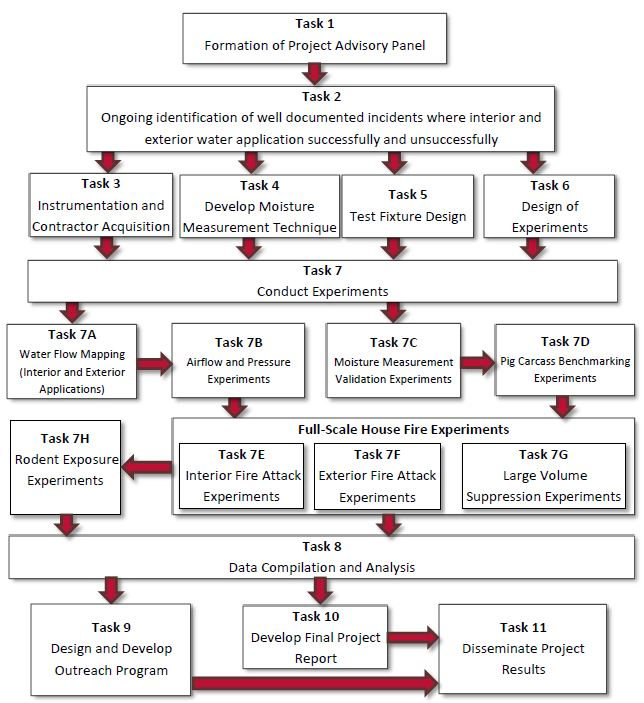
\includegraphics[width = 6in]{Figures/General/Flow_Chart}
% 	\caption{Project Technical Plan Flow Chart}
% 	\label{fig:TechPlanChart}
% \end{figure}

% \clearpage

% \item \textbf{Task 1 – Formation of a Project Advisory Panel}
% \normalfont
% \vspace*{\baselineskip}

% Task 1 will bring together an advisory panel of technical experts in the fire service; and fire service research field. An open application process will be administered to find fire service experts in fire stream application and training in fire attack methods. Representatives from organizations including: CFD (Chicago Fire Department), FDNY (Fire Department of New York), IAFC (International Association of Fire Chiefs), IAFF (International Association of Fire Fighters), NVFC (National Volunteer Fire Council), NIST (National Institute of Standards and Technology), and career and volunteer representatives from urban, suburban, and rural fire departments will be invited to participate. Invitations will also be extended to representatives of major fire service publications and training material publishers. This well rounded panel allows UL to ensure their research is directed to the target audiences and that the end product of the research is able to be easily disseminated into practice.
% \vspace*{\baselineskip}

% \item \textbf{Task 2 – Incident Review}
% \normalfont
% \vspace*{\baselineskip}

% Task 2 is to leverage our fire service advisory panel to conduct an extensive search to find examples of well documented successful and unsuccessful interior and exterior fire stream applications. This will be completed by monitoring fire service websites for videos and after action reports where there are defined flow paths and clear fire service fire attack actions. With approval of the fire department these incidents will be examined in detail to determine the impacts of fire stream type, flow, pattern and placement on the outcome of the incident, firefighter safety and victim injuries if applicable. Everyday the fire service is learning through their own experience and the experience of others through the means of sharing video. To make sure our experiments are tied in best with common fire service experiences we will identify trends in these incidents and tie the research results to the experience or beliefs gained from these incidents.
% \vspace*{\baselineskip}

% \item \textbf{Task 3 – Test Supplies, Instrumentation and Contractor Acquisition}
% \normalfont
% \vspace*{\baselineskip}

% Task 3 will allow for UL to acquire research supplies and instrumentation to complete this project. Instrumentation includes thermocouples to measure thermal conditions that potential victims or firefighters would be exposed to, differential pressure sensors and bidirectional probes to measure pressure and gas velocity throughout the test fixtures, bullet cameras to capture interior views of the test fixtures to provide visual evidence of conditions. Other test equipment such as data loggers, gas analyzers, thermal imaging cameras and video cameras were acquired from previous studies and will be utilized during this study. A contractor will also be selected to construct the test house structures using construction practices representative of what would be found in most neighborhoods across the country.
% \vspace*{\baselineskip}

% \item \textbf{Task 4 – Develop Moisture Measurement Technique}
% \normalfont
% \vspace*{\baselineskip}

% During this task different commercially available moisture measurement technologies will be examined for their ability to make moisture measurements in conditions that will be created in the full-scale house experiments. These conditions include elevated temperatures and a high density of particulate. This measurement will allow for the ability to map where steam travels in the structure to assess the impact of steam on fire victims and on fire service steam burns.

% Several well established instruments exist to characterize the environmental conditions within a structure containing fires by measuring a variety of effluent gases along with temperature, heat flux and flow characteristics. However, the ability to measure moisture content in conditions applicable to describing fire environments, particularly after water has been applied to suppress the fire, is not presently available. The effect of measuring moisture at elevated temperatures is critical for hazard assessments for both firefighters operating within a structure and potential victims who are trapped in the structure. In the SFPE Handbook, Purser suggests that: “… it is possible that the presence of water vapor may be an important neglected hazard in fires”, and, “Humid air, steam or smoke with a high thermal capacity of latent heat (due to vapor content or suspended liquid or solid particles) may be dangerous at temperatures of around 212~$^{\circ}$F (100~$^{\circ}$C), causing burns throughout the respiratory tract. It may be possible to predict the likely effects of hot-smoke atmospheres if thermal capacity or latent heat were measured.” 

% Thus, the ability to measure moisture concentration in such environments is a critical avenue of research for firefighter safety as well as to fully understand the impact of tactical decisions on trapped victim safety. It is of particular importance to know the moisture content in the rooms adjacent to the fire room at the level of occupants crawling on the floor (1~ft above the floor) or on furnishings (3~ft above the floor). Based on past experimental results, the temperatures observed at these levels in rooms adjacent to the fire room are typically under 400~$^{\circ}$F.  

% Commercially available moisture sensors have been developed recently for industrial process control, but these have not been studied for applicability to the live fire conditions. At the University of Illinois, Professor Dimitrios Kyritsis’ lab has advanced multiple techniques based on electrical and laser based measurements of gases during internal combustion engine operation that can be adapted to the sooty, dynamically changing live-fire environment. While there are a large number of techniques to measure moisture, most are inapplicable to the situation of high temperature moisture measurements in a combusting environment. Two techniques that could have use in these types of environments are infrared absorption techniques and electrical impedance techniques. There are two different methods to measure moisture using electrical impedance, resistive methods and capacitive methods. Both methods measure the relative humidity of the environment. Each method has its own set of advantages, with the resistive methods having a faster response time, while the capacitive methods can resolve relative humidity measurements all the way to 0\% RH. It is for this reason that the capacitive methods are most useful for this application, since at temperatures around 400 oF and volume percent of H2O under 10\%, the relative humidity will be under 1\% RH. Resistive methods do not accurately measure relative humidity under 5\% RH.  

% Absorption spectrometry is another possible technique for measuring moisture content in harsh, high temperature environments. Water has several absorption bands in the near-infrared range, which allows the use of tunable diode lasers to measure the moisture content. With proper thermal and optical control of the laser source and sample train such a technique should be operable at temperature exceeding 1800~$^{\circ}$F, be able to operate in and compensate for sooty and smoky environments, and have a very rapid response time on the order of seconds. Such approaches have been utilized to perform in-situ analysis from controlled combustion and process exhaust systems. However, due to the nature of the live-fire experiments studied here, an extraction technique may have to be implemented. Such techniques will be designed and tested at the University of Illinois at Urbana-Champaign prior to the full-scale tests.
% \vspace*{\baselineskip}

% \item \textbf{Task 5 – Test Fixture Design}
% \normalfont
% \vspace*{\baselineskip}

% Task 5 is the design of the test fixtures to be used in the experiments. The main test fixtures will be two single family residential home (1200 ft$^2$ single story ranch house) to be constructed in UL’s Large Fire Facility. This is the near the same design built for the three previous ventilation research grants and will therefore allow continuity of previous results to expand our knowledge. One of the main test fixtures will be altered to constructed an open floor plan so that gas cooling can be analyzed in different volumes. The test fixture will be furnished with contents that is representative of common households and refurnished after each experiment. Additional test fixture details are provided in the Appendix.
% \vspace*{\baselineskip}

% \clearpage

% \item \textbf{Task 6 – Design of Experiments}
% \normalfont
% \vspace*{\baselineskip}

% Task 6 is the design of the experiments. In this task UL’s project engineers will work closely with the advisory panel to ensure fire service concerns are addressed and that the results will be of great benefit to the end users. All experimental variables, equipment, personnel, infrastructure and other resources will be evaluated to determine the best set of experiments to get the most for the investment and provide the largest return to the fire community. Variables such as types of nozzles, flow rates, nozzle patterns, ventilation parameters, timing of tactics, ignition location, and fuel loading will be discussed and selected during a technical panel meeting.  
% \vspace*{\baselineskip}

% \item \textbf{Task 7 - Conduct Experiments}
% \normalfont
% \vspace*{\baselineskip}

% \subitem \textbf{Task 7A:  Water Flow Mapping (Interior and Exterior Applications)}
% \normalfont
% \vspace*{\baselineskip} 

% Methodology: Conduct a series of experiments in a compartment constructed to determine where water goes once discharged from fire department nozzles during a simulated interior fire attack and exterior fire attack. The ability to suppress a fire safely and efficiently is dependent on how much water absorbs energy from the fire and what surfaces are cooled. A combination of water mapping techniques that are commonly used for characterizing sprinkler sprays will be utilized to determine flow distribution. The compartment will be of similar size to the fire rooms in the full-scale fire experiments so that the results can be linked.

% Water will be flowed utilizing common fire department nozzles with 3 patterns (combination nozzle in a straight stream pattern, combination nozzle in a narrow fog pattern and a smooth bore nozzle pattern). Different nozzle techniques that are commonly taught to firefighters and utilized in practice will be evaluated such as circular motions, z patterns, flowing off the ceiling and flowing ahead. Common flow rates for each nozzle will be used during the experiments. We will also calibrate our remote water delivery method that will be utilized during Tasks 7E and 7F to distribute the water in a repeatable manner to what would be done by firefighters. Several experiments will be done in triplicate to examine repeatability.  

% Measurements: The actual delivered density apparatus (described later) will be used to determine water distribution, video cameras will be used to document the nozzle techniques and gross water distribution. Data from this Task will be analyzed and used to design the experiments described in Task 7E, 7F, and 7G.
% \vspace*{\baselineskip}

% \subitem \textbf{Task 7B:  Air Flow and Pressure Experiments}
% \normalfont
% \vspace*{\baselineskip}

% Methodology: Conduct air flow and pressure experiments in the test fixtures prior to the introduction of any fire. Different hose streams and nozzle movement techniques entrain different amounts of air which can greatly impact fire dynamics, firefighter safety and victim survivability. The same nozzles, stream types and nozzle techniques will be used as Task 7A and the amount of air flow created and pressures generated in the structure will be measured. Different flow paths will also be established to see their impact such as having a ventilation point ahead of the hose-line and having no ventilation opening ahead of the hoseline. We will also examine air movement generated by 1 ¾ in., 2 ½ in. hand-lines and flows from master-stream devices (deck gun and ladder pipe).

% Measurements: During each of these experiments, velocities will be measured with anemometers and bidirectional probes attached to differential pressure gauges. Pressures will be measured with differential pressure gauges and HVAC air balancing measurements will be made. This data will allow for the analysis of air movement and its impact on fire growth measured in Tasks 7E and 7F.
% \vspace*{\baselineskip}

% \subitem \textbf{Task 7C:  Moisture Measurement Validation Experiments}
% \normalfont
% \vspace*{\baselineskip}

% Methodology: The candidate moisture measurement techniques identified in Task 4 will be validated by this series of experiments. A bench scale apparatus will be designed and constructed that will allow the team to carefully calibrate moisture concentrations at temperatures up to 500~$^{\circ}$F and in the presence of potential confounders such as typical fire effluent gases and dense smoke conditions. A closed loop flow bench will be designed with a radiative heating element and moisture injection ports allowing adding controlled volumes of moisture to initially dry room air. These ports will also allow controlled metering of CO and CO2 as well as fire smoke effluent collected from live-fire burn experiments.

% Measurements: Moisture percentage will be measured and compared against controlled ambient conditions. Initial measurements will be made in a controlled environment with known temperature and moisture concentrations up to 500~$^{\circ}$F, (max 3~ft temperatures in bedrooms found in the Vertical Ventilation Study (source***)). After validation in these environments, a controlled concentration of potential confounders will be added to the test bench included typical fire gases (CO2, CO) and varying soot concentrations.
% \vspace*{\baselineskip}

% \subitem \textbf{Task 7D:  Pig Carcass Benchmarking Experiments}
% \normalfont
% \vspace*{\baselineskip}

% Victims trapped within a structure face the risk of thermal burn injuries, particularly with unprotected skin. Suppression activities by the Fire Service can reduce this hazard by removing the heat source producing these dangerous conditions, however, the additional risks encountered by the conversion of water to steam must be studied. The risk for moisture related skin burns is likewise present for firefighters applying water to burning materials from inside the structure. While firefighting PPE provides a significant measure of protection, burn injuries are still a significant hazard during interior firefighting operations.

% The dangers of thermal injury from exposure to heat and products of combustion and time-temperature characteristics required for skin burns has been researched for several years. Typical studies involve exposing skin to a controlled thermal exposure and the time to an outcome, such as dermal or epidermal temperature changes or visual indications of damage. The synergistic effect of elevated temperature and moisture content on skin is conceptually understood due to the large latent heat and partial pressure of water at temperatures above 140~$^{\circ}$F. However, the effect of suppression tactics and the rapidly changing transient nature of exposure during this time frame (ambient temperature reducing, moisture content increasing) on risk for skin burns has not been measured in response to realistic fire suppression experiments. 

% Most commonly, porcine skin is used as a surrogate for human skin in burn studies (source**) as pig skin is more human like than any other readily available animal (source***). Furthermore, epidermal and dermal thicknesses for 3-4 month old swine are similar to an average human is estimated to be 70~µm, and 2-3~mm. Pig carcasses have been successfully utilized in place of live animal studies in part because the water loss from the skin of a live pig does not differ significantly from a carcass (source**).

% Methodology: In order to better understand burn injuries to both firefighters and potential occupants pig carcasses will be placed in various target rooms at different locations (1~ft and 3~ft from the floor) near the moisture sampling measurements during the house fire experiments. Pig carcasses will be obtained through the University of Illinois College Of Veterinary Medicine after they have completed their research tasks at the University. The 3-4 month old pigs will be of similar weight and have skin thickness (epidermal layer ~60-80~µm, dermal thickness of 1-3~mm) that is comparable to human skin and can be analyzed as a surrogate for potential human skin damage. Prior to inclusion in the live-fire structure, samples will be exposed to varying levels of radiant and convected heat with controlled moisture content to establish a baseline for comparison of damage as a function of exposure.  

% Measurements: Thermocouples will be sewn onto the skin surface and under the pig’s dermal layer using sutures to measure temperature gradient and establish the time line for first degree (skin surface at 113~$^{\circ}$F) and third degree (sub-dermal temperatures reach 113~$^{\circ}$F). In the scenarios where sections of the pig will be covered by firefighting PPE, temperature and relative humidity (to measure penetration of moisture through the PPE) will be measured on the exterior and interior of the clothing in the same area. Using the instrument developed and validated in Task 7C moisture concentration will be measured in the immediate vicinity of the exposed pig. Skin damage will be well documented visually for comparison with the carcasses utilized in Tasks 7E-G.
% \vspace*{\baselineskip}

% \subitem \textbf{Task 7E:  Interior Fire Attack Experiments}
% \normalfont
% \vspace*{\baselineskip}

% Methodology: A series of 12 full-scale house fire experiments will be conducted with simulated interior fire attack. The house will be furnished with modern furnishings and each experiment will have identical content.  A fire will be ignited in the master bedroom and the flow path will be altered to simulate scenarios that the fire department would arrive to or that would be created by fire department operations. The first 6 experiments will examine fire department arrival to a closed house with a ventilation limited fire. The front door will be opened creating a flow path. This will be repeated 5 times, utilizing 2 different hose streams, a controlled door, a coordinated ventilation opening, and once with no water application.  

% Five victim locations will be instrumented and the flow path the suppression crew would be advancing through will be instrumented to examine conditions that the crew would be exposed to. The hosestream will be applied utilizing a monitor nozzle that will be able to advance on a set of tracks and will be programmed to flow the desired pattern and motion. The second set of experiments will add a second flow path by ventilating the master bedroom window. This will increase the size of the fire but will provide a low pressure point opposite of the suppression crew. This will be repeated 5 times with two different hose stream patterns, two different hose line advances, and once with no water application until the front door flow path closes up and fire extends out of the front door. A third set of experiments will add a third flow path through Bedroom 2. Again 2 different hose stream patterns will be examined, two difference advances will be tested, and one experiment where no water is applied until fire extends out of the front door of the structure.

% Measurements: Measurements will be made to examine the fire dynamics in the test fixture, the exposure to firefighters in the flow path and to potential victims in several locations. The test fixture will be instrumented to measure temperature in every room, gas concentrations, pressure, gas velocity, thermal imaging and digital video. These measurements will allow for quantification of fire behavior, the impact of the water application and tenability for firefighters and occupants. Five victim measurement packages will be placed in the test fixture.  The packages will consist of temperature measurements at multiple elevations, gas concentration measurements (oxygen, carbon monoxide and carbon dioxide), heat flux with water conditioned to 98 degrees to get more accurate heat transfer to skin, an instrumented pig carcass, a moisture measurement device and a video camera. 
% \vspace*{\baselineskip}

% \subitem \textbf{Task 7F:  Exterior Fire Attack Experiments}
% \normalfont
% \vspace*{\baselineskip}

% Methodology: A series of 6 full-scale house fire experiments will be conducted with simulated offensive exterior fire attack. A fire will be ignited in the master bedroom and the flow path will be altered to simulate scenarios that the fire department would arrive to or that would be created by fire department operations. The first 4 experiments will examine fire department arrival to fire extending out of the master bedroom window. Water will be applied through the window, utilizing 3 different hose streams. Five victim locations will be instrumented to examine conditions that they would be exposed to. The hose stream will be applied utilizing a monitor nozzle that will be programmed to flow the desired pattern and motion. The second set of experiments will add a flow path by ventilating the Bedroom 2 window. This will increase the size of the fire and will allow it to begin to spread into Bedroom 2. This will be repeated 3 times with three different hose stream patterns and once with no water application. A third set of 2 experiments will ignite the fire in the master bedroom and Bedroom 2 with both of their windows open (Figure 10). Once fire is extending out of both bedroom windows 2 different hose stream patterns will be examined by flowing water into the master bedroom window.

% Measurements: Same measurements as Task 7E, Interior Fire Attack Experiments.
% \vspace*{\baselineskip}

% \subitem \textbf{Task 7G:  Large Volume Suppression Experiments}
% \normalfont
% \vspace*{\baselineskip}

% Methodology: A series of 8 experiments will be conducted that are the same as the first 8 interior fire attack experiments with the exception that all of the interior walls in the test fixture will be removed except for the walls to the master bedroom (Figure 11 and Figure 12).  This increased volume will allow for the analysis of gas cooling as a result of indirect attack in an open floor plan when the fire can not be accessed with the hose stream without crawling into the structure through the flow path. The fire will be allowed to develop until temperatures in the large volume would require an advancing suppression crew to cool the upper gas layer in order to advance to the bedroom fire.  The advancing crew will be simulated just as in Task 7E so that the 2 configurations can be compared, compartmented floor plan versus modern open floor plan.

% Measurements:  The test fixture will be instrumented to measure temperature in every room, gas concentrations, pressure, gas velocity, thermal imaging and digital video. Four victim locations will be instrumented to examine conditions that they would be exposed to. These measurements will allow for quantification of fire behavior, the impact of the water application and tenability for firefighters and occupants. The data will be analyzed and compared to the compartmented measurements from Task 7E.
% \vspace*{\baselineskip}
 
% \item \textbf{Task 8 – Data Compilation and Analysis}
% \normalfont
% \vspace*{\baselineskip}

% Task 8 is the compilation and analysis that will be conducted by UL engineers to make the data usable by the fire community. The data will be organized in graphs that will be reviewed by the technical panel in preparation for the final report and the online training program. The focus of the analysis will be to calculate tenability conditions for potential victims and firefighters during each of the scenarios. In addition, tactical considerations will be developed in conjunction with the fire service advisory panel. Each of these considerations will be supported by data, experimental video evidence and actual fire incidents documented in Task 2 and incorporated in the technical report and outreach program.
% \vspace*{\baselineskip}

% \item \textbf{Task 9 – Design and Develop Outreach Program}
% \normalfont
% \vspace*{\baselineskip}

% In task 9, UL engineers will work with instructional designers to produce an interactive training program for the fire community. The final program will be shared via the www.ULfirefightersafety.com website, www.Modernfirebehavior.com website, and UL FSRI Social media accounts free of charge to the fire service. The course will be consistent with previous courses developed by UL as shown in the figures below. The course will contain data, pictures, video and professional narration and allow firefighters of all levels to navigate through the course at their own speed. This program will include linkages to tactical considerations learned from the previous three studies on horizontal, vertical and positive pressure ventilation and the Governor’s Island experiments completed in partnership with FDNY and NIST.
% \vspace*{\baselineskip}

% \item \textbf{Task 10 – Develop Final Project Report}
% \normalfont
% \vspace*{\baselineskip}

% Task 10 is the development of the final report that details all of the experiments and results. The report will be provided to DHS and made publicly available via UL’s website for the fire service, www.ULfirefightersafety.com to serve as a reference for future research. The tactical considerations developed with the technical advisory panel will be a focus within the report. A fire service summary report will also be written and disseminated that includes critical information for firefighter safety.
% \vspace*{\baselineskip}

% \item \textbf{Task 11 – Disseminate Project Results}
% \normalfont
% \vspace*{\baselineskip}

% Task 11 is the dissemination of the research results. Results are shared by presenting in venues such as the National Fire Protection Association Annual Conference, Fire Department Instructors Conference, International Association of Fire Chiefs Fire Rescue International, and the International Association of Fire Fighters Annual Conference. These venues provide a large number of attendees from the fire service and research communities and are a formal means to disseminate the results of the study. Additional dissemination will include publication in fire service trade magazines and peer reviewed journals. As with previous outreach results, videos and presentation content will be made available at request to be used for local dissemination and for train the trainer programs. Continued dissemination is achieved by making the final project report and online training program available via UL’s websites for the fire service, www.ULfirefightersafety.com and www.Modernfirebehavior.com. We will also share project results on our and our partners social media channels, Facebook, Twitter, YouTube and our Fire Engineering Radio Show, “Research to Tactics.”
% \vspace*{\baselineskip}

% \end{itemize}

\clearpage

\section{Scope}
This study looked at the impact the two main methods of fire attack, interior and transitional, have on victim survivability in residential structures. Due to the significant number of variables on a structure fire, limitations exist in the ability to evaluate them all. The variables selected were chosen to begin to bound the problem and provide insight into the practical application of fire suppression methods. 

These variables included house geometry, fuel loading, fire department arrival time, tactical choices, hose stream flow rates, and ventilation locations. The house geometry included a single story 1,600~ft$^2$ ranch style home with long residential hallway to evaluate the impact of approaching a fire down a hallway. The bedrooms were all located off the long hallway with the fire rooms at the far end.  Intervention times were based on fire department personnel arriving after the fire became ventilation limited. By bounding these variables and controlling the test conditions during firefighting operations, it was possible to evaluate the impact of different fire suppression tactics on fire dynamics and conditions inside a single family.  

The study did not include differences in hose line deployments. The line was deployed to front of structure for first action, advancement through the front door or transitional attack through the front window. The line was charged, and pressure, flow and nozzle position were all checked and set prior to the start of the experiment. The study also did not include evaluation of crew size on timing. The suppression crew consisted of three firefighters, a nozzle firefighter, a backup firefighter and a line advancement firefighter. The firefighters in these positions were consistent though out all the experiments. Additionally, the hose streams were flowed from pre-determined positions to evaluate the impact of different tactics, be it transitional (through the window) or interior (down the hallway). Flow based on conditions only occurred when the suppression crew felt it was necessary for their safety. 

The fires in this study were content fires and represented a fire event within the living space of the home, and not a structure fire with fire extension into the walls or attic space.

\section{Limitations}
Recreating all the variables of a fire department response is a challenge due to the complex nature of a fire scene. Research into the effectiveness of various suppression tactics is not intended to recreate the fire scene in its entirety but to fix as many of the variables as possible to permit a scientific comparison. 

This project was conducted solely in a laboratory facility in order to fix the environmental conditions (wind, rain, temperature and pressure). During a fire department response, the environmental conditions will play a role in tactical choices. The Tactical Considerations from this study need to be evaluated against the conditions the fire department is faced with at the time. 

The location of the measurements for victim survivability were chosen to compare the effects of proximity to the fire, being behind a closed door and being elevated off the floor. Although these values can be extrapolated to other similar locations within the structure, due to the complexity of the fire environment, they are not representative off all the possible locations a victim may be located in a residential structure.  

It is important to note that measurement of quantities such as moisture content and burn potential are difficult in the fire environment. This study advanced these measurement techniques however not all experiments were successful in recording usable data with regards to these two values. The experiments were data was obtained have been analyzed and used to develop tactical considerations where applicable. Future research, utilizing these measurement techniques is necessary to fully understand the impact of specific fire suppression tactics. 

Additionally, the number of experiments was fixed based on the available budget. This project was not able to test all of the potential tactical choices of a suppression crew, thus it is important to utilize both these research results and your personal experience when making tactical choices.  

The tactical considerations developed are intended for similar size (1,620~ft$^2$) residential occupancies with similar compartment sizes (140-175~ft$^2$). Further research is required for larger residential structures (in excess of 3,000~ft$^2$), two story and commercial occupancies.

\clearpage

\chapter{Literature Overview}

Hose, nozzles and water have been used by the fire service for hundreds of years. Despite their frequent use, there has been little scientific research conducted on the effective use of these tools for fire suppression. It is common in the fire service to find discussions about which nozzle is better or which flow rate is required for what sized fire but this is based on experience and usually not science. 

In 1950 Chief Lloyd Layman presented a paper titled “Little Drops of Water” at the Fire Department Instructors Conference. He introduced what he called indirect method of attack to suppress interior building fires by using the heat absorbing properties of expanding and condensing steam, produced in great quantities by fog streams. The conclusions were based on Coast Guard experiments that Layman was in charge of conducting at the Coast Guard Firefighting School at Fort McHenry in Baltimore, MD. Layman continued his experiments after he returned to his position as fire chief in Parkersburg, WV where he applied his tactic in building fires.  This research had a very large impact on the fire service and their suppression techniques to this day. 

Throughout the 1950’s a National Committee began conducting experiments to collect data on the growth and behavior of interior fires and how to most effectively suppress them. Keith Royer and Bill Nelson were members of this committee, and as the heads of the firemanship training program at the Iowa State University’s Engineering Extension, they collected and analyzed data from hundreds of experimental fires. Through this research the fire service was taught about fire behavior and how to suppress fire with a combination fire attack. They examined the amount of heat generated by common fuels, the heat absorbing capacity of water, the impact of compartment volume during suppression and they developed the Iowa formula. The Iowa formula or critical rate of flow formula is still used today and it determines the amount of water needed to control a fire in the largest open space within a structure by dividing the cubic foot volume of the space by 100.

While the physics of fire development has not changed over time, the fire environment for specifically the single family home has evolved. Several factors including home size, geometry, contents and construction materials have changed significantly over the past 50 or more years. Each of these factors has impacted firefighter and occupant safety. Faster fire propagation, shorter times to flashover, rapid changes in fire dynamics and shorter escape times all impact fire service suppression techniques and effectiveness. Many of the variables in Royer and Nelson’s analysis have changed and more research is needed to see how suppression techniques used in the 1950’s with 1950’s fuel loads and firefighting tools translates to today’s firefighter safety and effectiveness.

Beginning in 1994, the Naval Research Laboratory carried out a series of full-scale fire experiments to compare straight stream attack versus fog pattern attack. These experiments were conducted on the Navy ship ex-USS Shadwell with a fire volume of approximately 110~m$^3$. In these experiments one 60 degree fog pattern was applied at a 45 degree angle into the smoke layer. They examined cooling effects, steam generation and thermal layer disruption. Their experiments examined shielded and non-shielded fires and concluded that using fog to cool the upper layer was more effective and safer than straight stream attack when the fire could not be attacked directly and the firefighters heart rates and body temperatures were lower utilizing the fog attack.

In 1998 NIST conducted a series of experiments to demonstrate the suppression effectiveness of water-based firefighting agents. This was a step toward creating test procedures to determine suppression effectiveness to develop a standardized test method for evaluating the fire fighting effectiveness of water and other agents. This study provides preliminary data upon which firefighting effectiveness test may be developed by it suggests additional research on application technique, tests reflective of the complexities found in firefighting and experiments involving structural-fire suppression.  

In 2002, The National Research Council of Canada conducted a literature search on 3D water fog techniques for firefighting. It discusses the impact of water fog characteristics associated with properties of the nozzle (e,g,, droplet size, momentum, flow rate, spray angle and pattern) and discharge techniques (e.g., discharge angle, and discharge duration related to the burns) on performance of the 3D water fog technique are discussed. This technique is to supplement a direct attack by controlling the environment the firefighters are in until they are in a position to apply water directly to the fire. Opponents of flowing water into smoke have concerns that include: (i) effectiveness of controlling the fire, compared to traditional straight stream attack; (ii) possible disruption of the thermal balance; (iii) possible generation of a large amount of hot steam that produces burn injuries to firefighters; and (iv) the performance of this technique is complex and requires extensive training. Advocates of this technique have attempted to respond to these concerns but very limited experimental studies have been undertaken do to complexity of the problems. Application techniques and fire conditions on the the performance of fog technique is not well studied and therefore there are little guidelines and adoption will be greatly limited.

Several theoretical studies had been conducted that examine droplet size and their ability to suppress fire gases. For example, when droplet diameter is reduced from 1000 nanometers to 100 nanometers the total surface area increases 10 times from 6 m2 to 60 m2 for 1 liter of water. Since these smaller droplets evaporate sooner, others have examined the lifetime of the droplet to determine how far it can travel based on temperature of the surrounding gases and droplet size. Further complicating this theory is that droplets all have an impact on each other as they turn to steam. Residence time can be further reduced compared to an individual droplet, because leading droplets impart forward momentum to the surrounding gas, reducing the air drag on the following droplets and resulting in better penetration. In 2010, the University of Maryland examined spray characteristics from fire hose nozzles. They examined the breakup of a smooth bore nozzle utilizing techniques such as shadowgraphy and a patternator and concluded that more research was needed to fully understand the water spray from fire hose nozzles.  

In 2000, Lund University examined the demand for extinguishing media in manual firefighting. They examined critical flow rates required to suppress fires by reviewing available literature and conducted a series of experiments that examined suppression of wood pallets at a fire training academy. They examined the five ways that water can be applied during fire extinguishment, on hot gases, on flames, on burning fuel, on fuel that is not yet burning and on hot surfaces. They highlight that what is most effective against the fire is not necessarily best for the firefighters since there are other constraints during firefighting operations such as limited air supply and multiple priorities. The optimum flow rate corresponds to an optimum control time, a control time that gives the lowest total demand for resources. Most of the current data for optimum water flow rate include experiments utilizing wood cribs or pallets, but not todays synthetic fuel loads in actual structures.  These studies also did not investigate the effect of flow paths or the impact of steam generation on firefighters or victims.

In 2003, a fire service group at the Rockland County (NY) Fire Training Center conducted a series of tests in their concrete training building. They measured the amount of air moved by solid bore and combination nozzles using common fire ground methods. They concluded that air volumes moved by smooth bore nozzles and combination nozzles in the straight stream setting are very similar if not the same, and that combination nozzles in the fog pattern move significant amounts of air which can over pressurize the fire area and send steam over the suppression crew even with a ventilation opening opposite the suppression crew. These tests were performed either with no fire or with a training fire but which are very different than actual fire conditions. Their tests do provide a good range of airflows that can be expected in our experiments. The authors state, “Our nozzle testing program was not as controlled and as precise as we would have liked.” They also did not have measurement devices that were able to accurately measure air flows from a fog pattern.  

The Firefighting Technology Group at NIST has a current project that is examining hose streams. This project examines a variety of fire fighting hose stream characteristics related to flow, distribution and thermal impact from both solid and fog stream nozzles. A series of real scale, laboratory based experiments have been started to look specifically at the water discharge and distribution characteristics, the impact of hose streams on a hot gas layer in a compartment, the impact of hose streams on gas flows through multi-compartment structures, and the suppression effectiveness on burning piles of wooden pallets. The proposed project will build on their results by utilizing real-scale structures with common residential fuels and making additional measurements to better characterize the impact of flow path, nozzle technique and steam generation on fire dynamics, firefighter exposure and occupant survivability.

\section{Fire Service Publications}

TECHNICAL PANEL, PLEASE PROVIDE RELEVANT WORK YOU FEEL SHOULD BE INCLUDED IN THE BACKGROUND FOR THIS STUDY

\section{Fire Service Training Manuals}

TECHNICAL PANEL, PLEASE PROVIDE RELEVANT WORK YOU FEEL SHOULD BE INCLUDED IN THE BACKGROUND FOR THIS STUDY

\section{Firefighter Line of Duty Deaths}

SECTION IN PROGRESS

\section{Research Work}

SECTION IN PROGRESS

\clearpage

\chapter{Experimental Configuration}
\label{chap:exp_config}

\section{Test Fixtures}

The full-scale fire experiments were conducted in two identical ranch structures, constructed in UL's Large Scale Fire Test Facility in Northbrook, IL. The test facility is a 120~ft x 120~ft by 60~ft high space with a concrete floor and movable ceiling. The space is provided with 60,000~CFM of exhaust capabilities though a regenerative thermal oxidizer (RTO) system which was running during each test. The make-up air for the system comes from make-up air ducts on the roof of the facility which run down the exterior walls to a grated vent opening at the floor level. Four total vents, two on each wall are balanced to evenly distribute the make-up air without creating air currents in the space. 

The test structures were designed to mimic the interior of a 1620~ft$^2$ ranch home. Figure \ref{fig:test_prop_photo} shows the Side A and Side C of the one of the test structures. They were designed by a residential architectural company to be typical of a single family home constructed in the late-20th century in the United States. The floor plan included 4 bedrooms, a bathroom, a living area, kitchen, and dining room. The bathroom and closet spaces were cordoned off and used as equipment spaces within the structure. Three of the bedrooms were left open during the fire experiments, while one bedroom (Bedroom 3) was left closed, to examine the impact of a closed door on fire behavior. The interior of the house had 8' ceilings, and the rooms were separated from each other with walls and doorways. The floor plan of the houses used for these experiments can be seen in Figure \ref{figure:ranchexp1_floorplan}.

\begin{figure}[H]
\centering
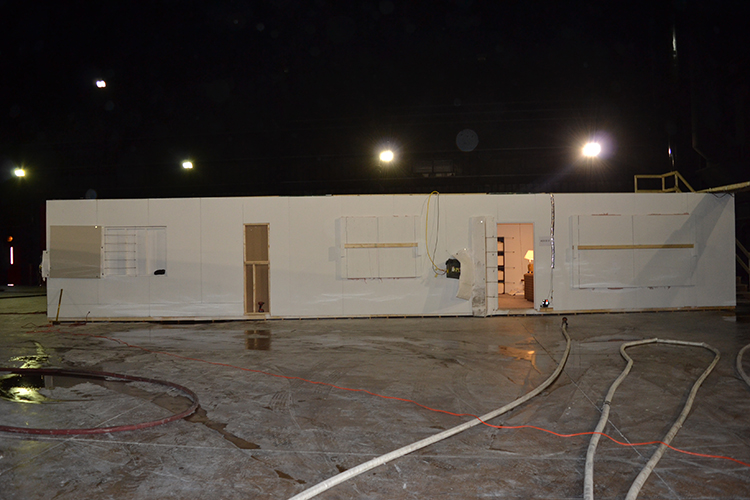
\includegraphics[width=0.45\textwidth]{0_Images/Ranch_Pictures/House_Front.jpg}
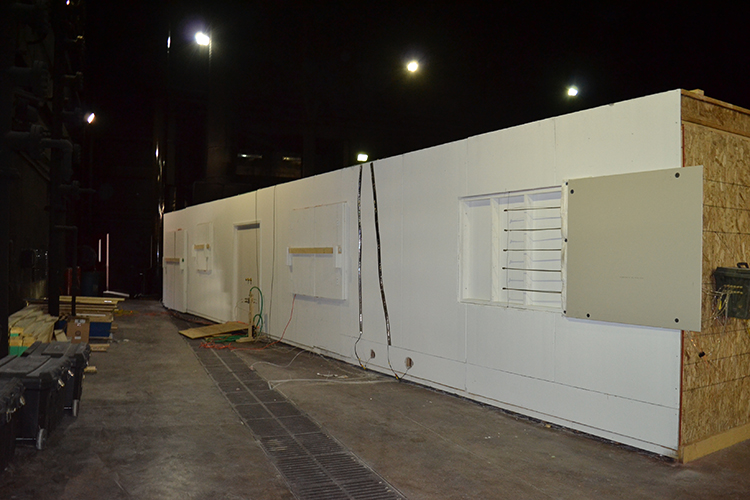
\includegraphics[width=0.45\textwidth]{0_Images/Ranch_Pictures/House_Rear.jpg}
\caption[Test Structure - Exterior Photos]{Exterior photos of test structure in UL's large fire lab. Side A (left) and Side C (right).}
\label{fig:test_prop_photo}
\end{figure}

The front door of the structure was a insulated metal door typical of a residential building. Windows of the fire rooms (Bedroom~1 \& Bedroom~2) were framed plugs with cement board on the interior face. All other windows were hinged pieces of OSB with fiberglass batt insulation on the interior to provide a seal. Window ventilation was intended to be a controlled action; thus windows/plugs were designed to remain in place during fire conditions. 
 
\begin{figure}[H]
\centering
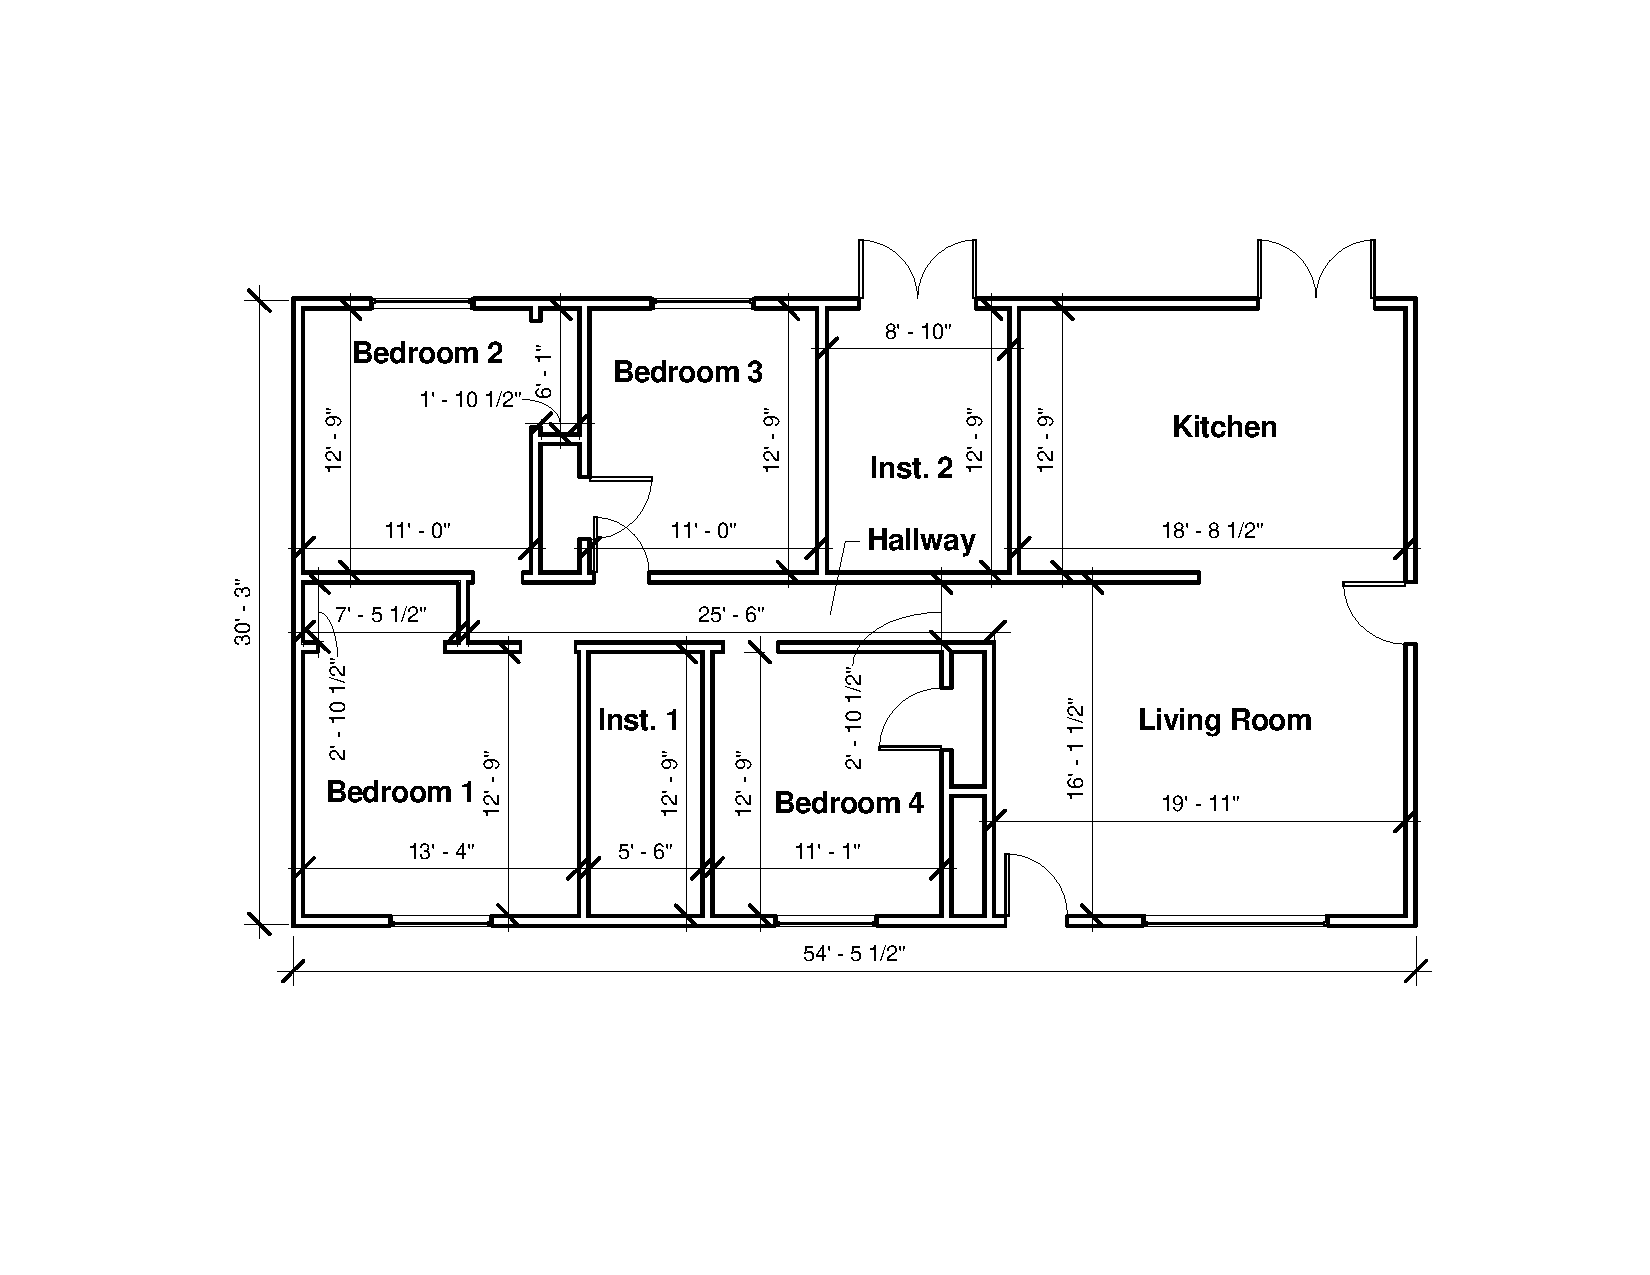
\includegraphics[width=0.9\textwidth]{0_Images/Ranch_Pictures/Floor_Plan}
\caption{Ranch Floor Plan}
\label{figure:ranchexp1_floorplan}
\end{figure}

Since the ranch fire experiments were intended to examine room and contents fires, and not structure fires, the walls of the fire rooms (Bedroom 1 \& 2), and hallway were lined with two layers of gypsum board: a surface layer of 1/2'' board and a base layer of 5/8'' board. The remaining interior surfaces in the structure consisted of 1/2'' drywall. The exterior walls were covered with cement board to limit exterior fire spread. The kitchen floor was composed of cement board, while the rest of the house was carpeted. 

\begin{figure}[H]
\centering
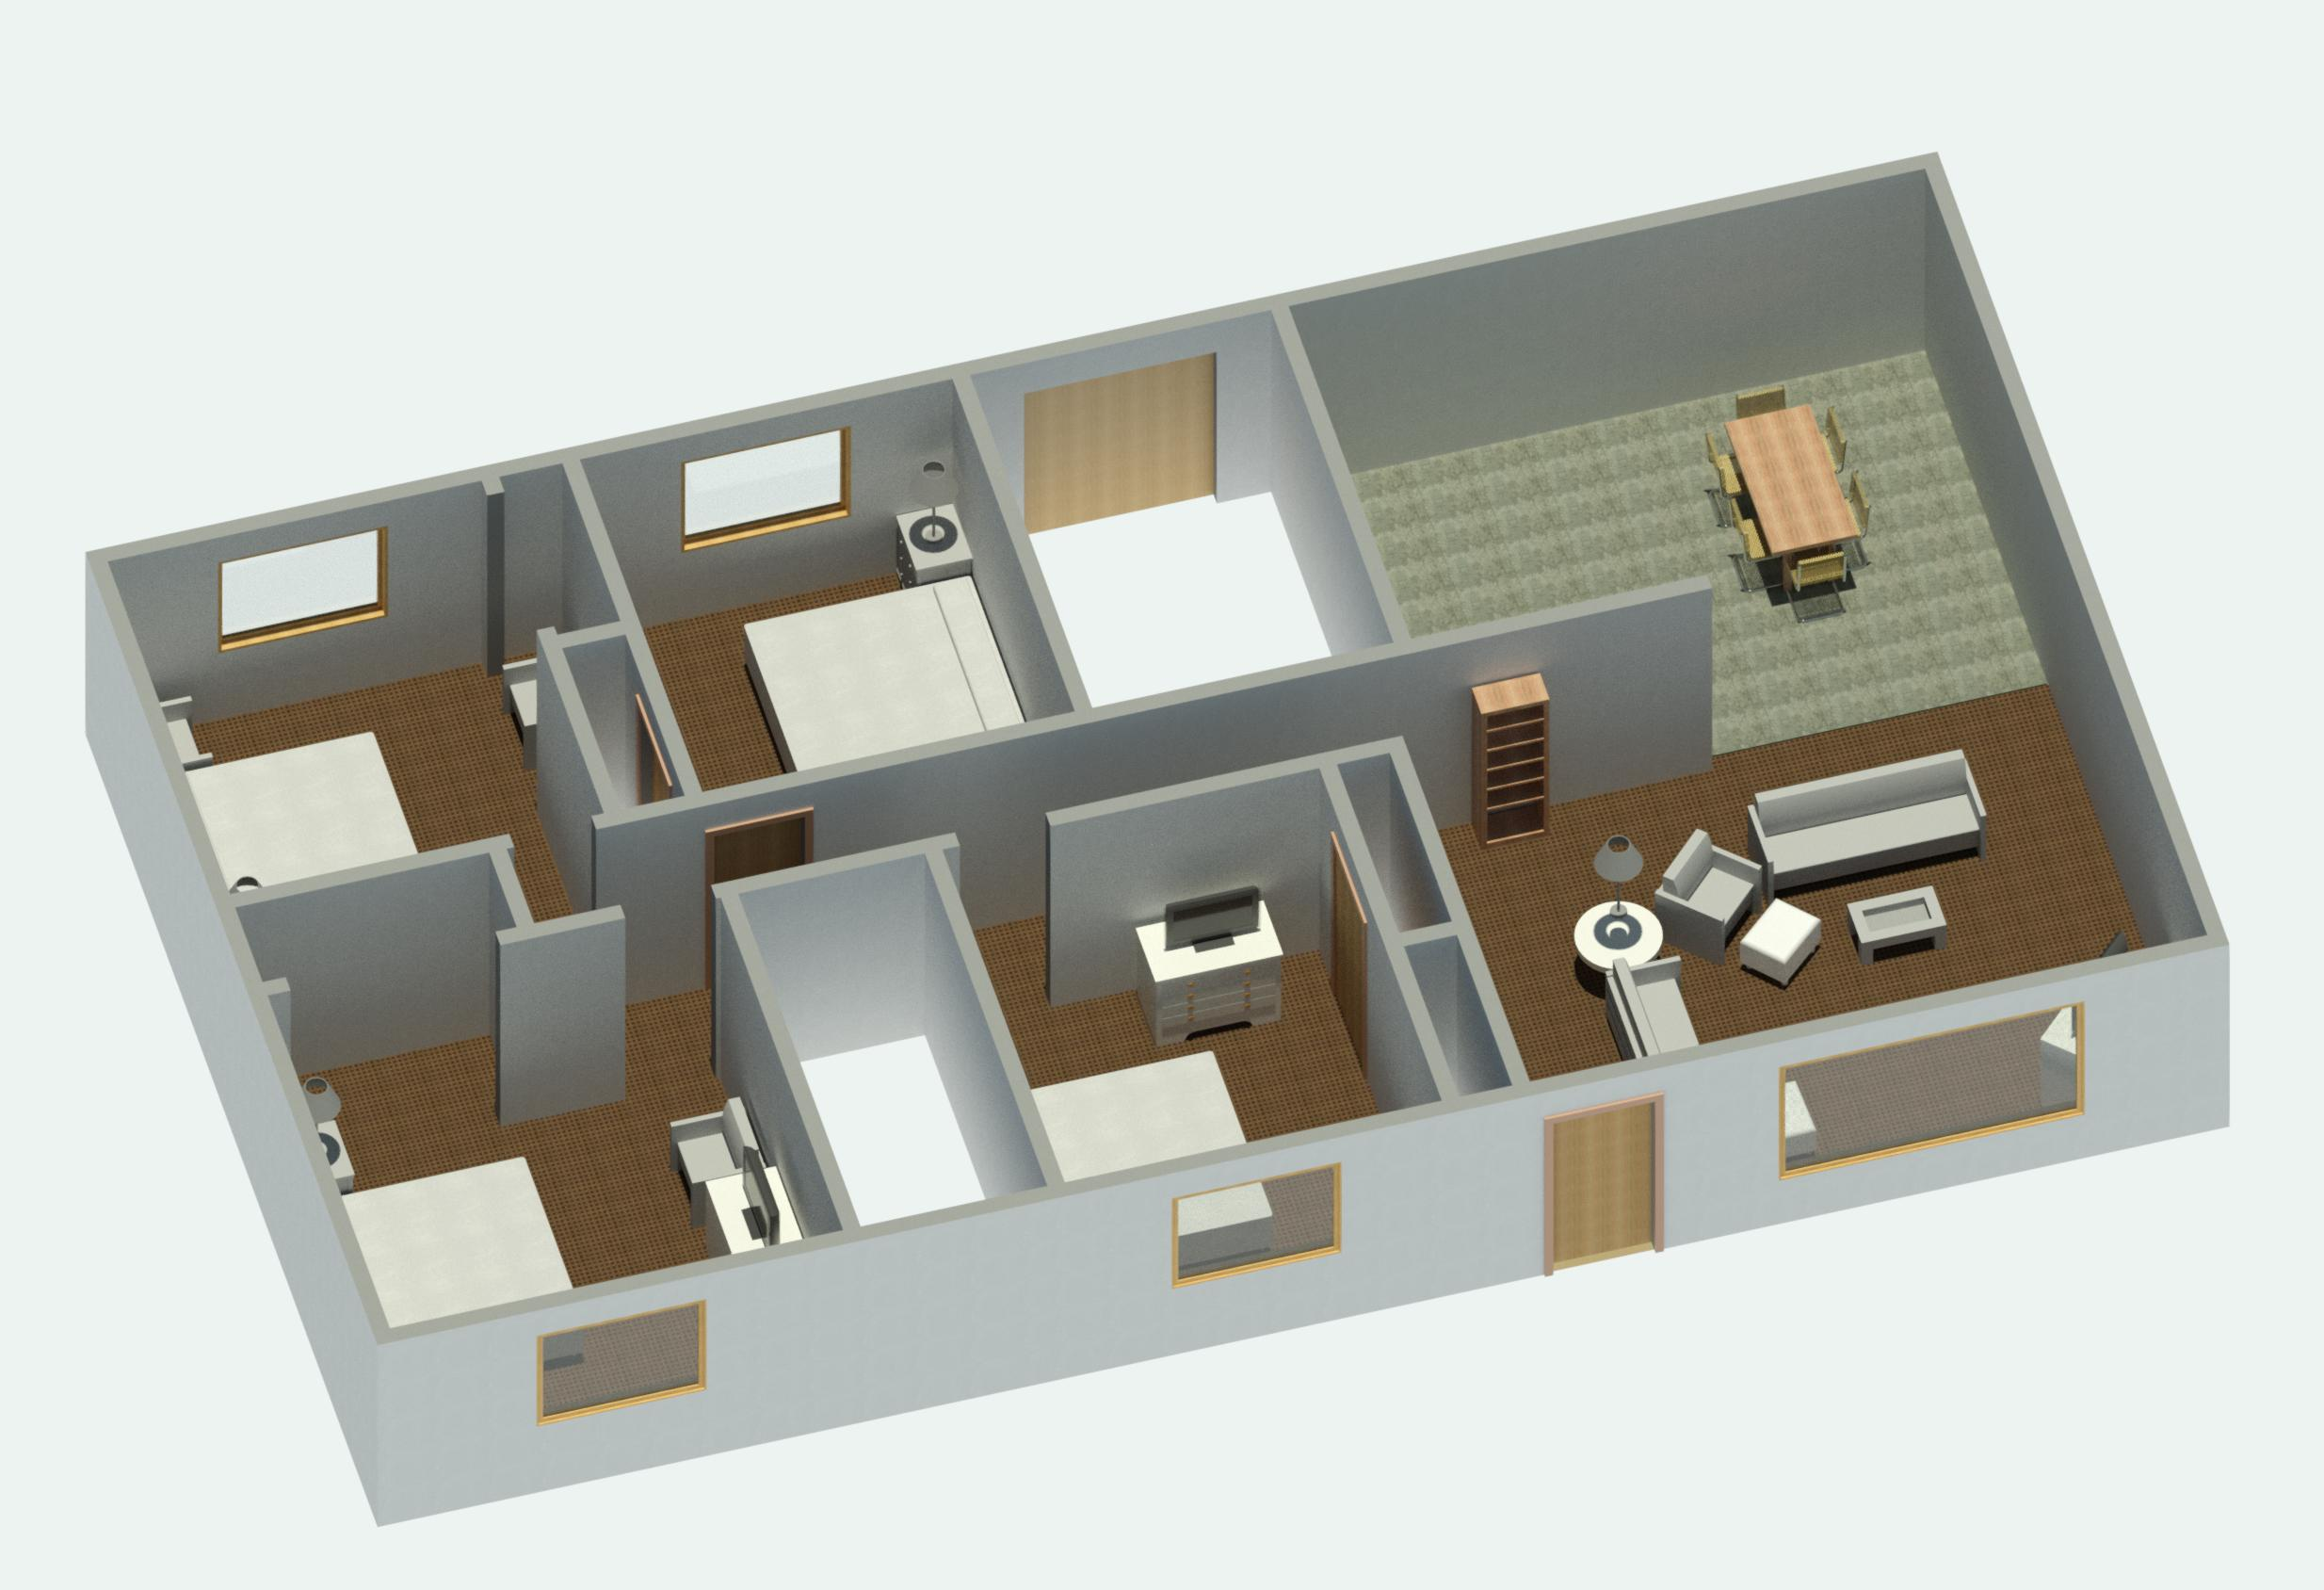
\includegraphics[width=.65\textwidth]{0_Images/Ranch_Pictures/Report_ISO_Furniture.jpg}
\caption{Furnished Experiment Layout}
\label{figure:ranchexp3_floorplan}
\end{figure}

\section{Fuel Loads}
Fuel loads were selected such that every experiment had the exact same configuration of fuel. The furniture was purchased from a wholesaler of re-purposed furniture, where necessary items such as comforters, polyurethane foam mattress toppers, and pillows were purchased new to ensure the same fuel load for each experiment. Figure \ref{fig:furniture_layout} shows the floor plan of the test fixture with the furniture included in each room. For detailed drawings of each room with furniture locations see appendix \ref{app:detailed_locations} The weights and dimensions for of the fuel load used for each experiment are listed in Table \ref{table:fuel_weights}.

\begin{figure}[H]
\centering
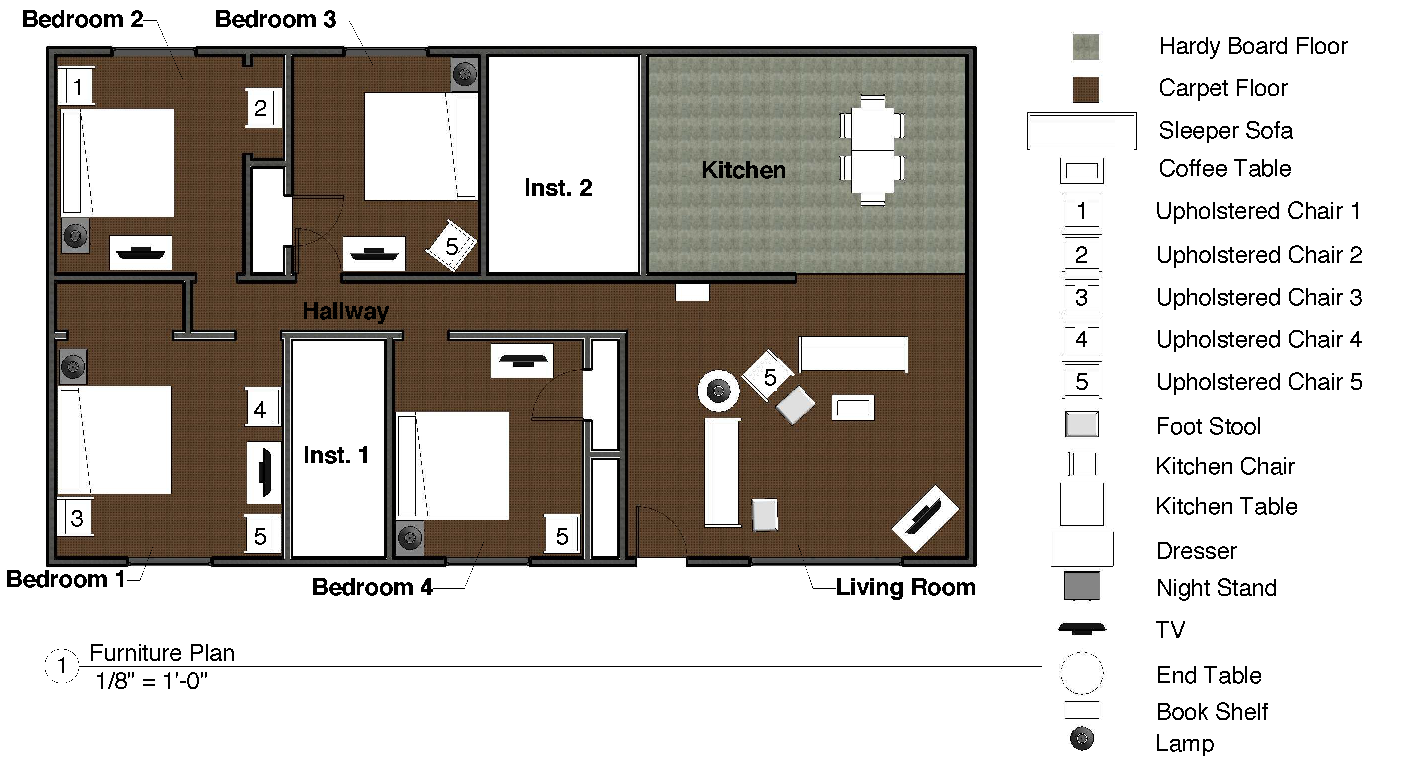
\includegraphics[width=0.95\textwidth]{0_Images/Instrumentation/Furniture_Plan.png}
\caption{Test Fixture Furniture Layout}
\label{fig:furniture_layout}
\end{figure}

\begin{table}[H]
\centering
\begin{tabular}{|L{0.23\textwidth}|C{0.08\textwidth}|C{0.08\textwidth}|C{0.08\textwidth}|C{0.08\textwidth}|L{0.37\textwidth}|}
\hline
Item 						&Length (in) 	&Width (in) 	&Height (in) 	&Weight (lbs.) 	&Material \\ \hline \hline
King Mattress 				&79 			&71 			&10 			&76 			&52\% Polyurethane Foam, 30\%, Blended Cotton Batting, \& 18\% Polyester Fiber Batting \\ \hline
King Box Spring 			&78 			&35 			&7 				&46 			&59\% Fiber Pad, 41\% Blended Cotton Batting \& Wood Frame \\ \hline
King Headboard 				&78 			&24 			&1 				&54 			&Medium Density Fiberboard \\ \hline
Pillow 						&23.5 			&17 			&4 				&1.5 			&Filling - All Polyester, Cover - 100\% Cotton \\ \hline
Comforter 					&104 			&92 			&1 				&4.6 			&Cover - 100\% Polyester, Fill - 100\% Polyester \\ \hline
Mattress Topper 4 in 		&78 			&75 			&3.875 			&16.0  			&Viscoelastic Polyurethane Foam Pad 100\% \\ \hline
Mattress Topper 5 in 		&77.5 			&76.25 			&4.625 			&20.1  			&Urethane Foam \\ \hline
Sofa Chair (Red Diamond) 	&35 			&35 			&34 			&69 			&Polyurethane Foam (Blended Cotton or, Polyester when used is less than 10\%) \\ \hline
Sofa Chair (Striped) 		&33 			&35 			&33.5 			&65 			&Polyurethane Foam 75\% Polyester Fiber 25\% \\ \hline
Sofa Chair (Yellow/Green) 	&31.25 			&31 			&39 			&54 			&Polyester Fiber 75\%, Polyurethane Foam 25\%, Pillow - Polyurethane Foam 90\%, Polyester Batting 10\% \\ \hline
Sofa Chair (Red Lines) 		&34.5 			&34 			&32 			&63 			&Urethane Foam 100\% \\ \hline
Sofa Chair (Red Swirl) 		&34 			&34 			&32 			&70 			&Blended Cotton Felt 100\%, Cushion, Polyurethane Foam 100\% \\ \hline
Night Stand 				&18 			&27 			&23.375 		&60 			&Solid Wood \\ \hline
Table Lamp Base 			&5.75 			&5.25 			&31.25 			&5.9 			&Glass, Metal  \\ \hline
Table Lame Shade 			&14.375 		&14.375 		&  				&  				&Cloth Shade \\ \hline 
Dresser 					&22.125 		&36 			&34.25 			&120 			&Wood \& Plywood \\ \hline
Curtain (Large) 			&107 			&73 			&0.125 			&13.7 			&Flame Retardant \& Synthetic Fibers \\ \hline
Curtain (Small) 			&39 			&73 			&0.125 			&4.5 			&Flame Retardant \& Synthetic Fibers \\ \hline
Sofa 						&35 			&77 			&30.5 			&255 			&Polyurethane Foam 50\%, Polyester Fiber 50\%,\& Wood Frame \\ \hline
Coffee Table 			 	&30 			&18 			&18.25 			&24.4 			&Particleboard \& Wood \\ \hline
End Table 			 		&24.25 			&24.25 			&22.125 		&32.1 			&Solid Wood \\ \hline
Footstool 					&19.75 			&25.5 			&16 			&21.3 			&Upholstery \\ \hline
Bookcase 					&11.5 			&24.625 		&71.25 			&46 			&Particleboard \\ \hline
Kitchen Table 				&52 			&26 			&24.5 			&29.1 			&Particleboard \& Wood \\ \hline
Straight Chair (Pink) 		&18 			&19 			&33 			&15.2 			&Wood \& Upholstery \\ \hline
Straight Chair (Blue) 		&19 			&19 			&38.875 		&14.9 			&Wood \& Upholstery \\ \hline
\end{tabular}
\caption{Fuel Load Information}
\label{table:fuel_weights}
\end{table}

\subsection*{Bedroom 1}
Bedroom 1 was furnished to simulate a typical bedroom in a residential home. The fuel load consisted of a king-sized bed, dresser, TV, nightstand, pillows, 4'' foam mattress topper, 3 stuffed chairs (1 Yellow/Green Chair, 1 Red Lined Chair, and 1 Red Swirl Chair), curtains, carpet, and carpet padding.  The orientation of the fuel can be seen in Figure \ref{figure:Bed1_fuel}. The fire was ignited remotely with an electric match in the seat cushion of the stuffed armchair at the side of the bed.

\begin{figure}[H]
\centering
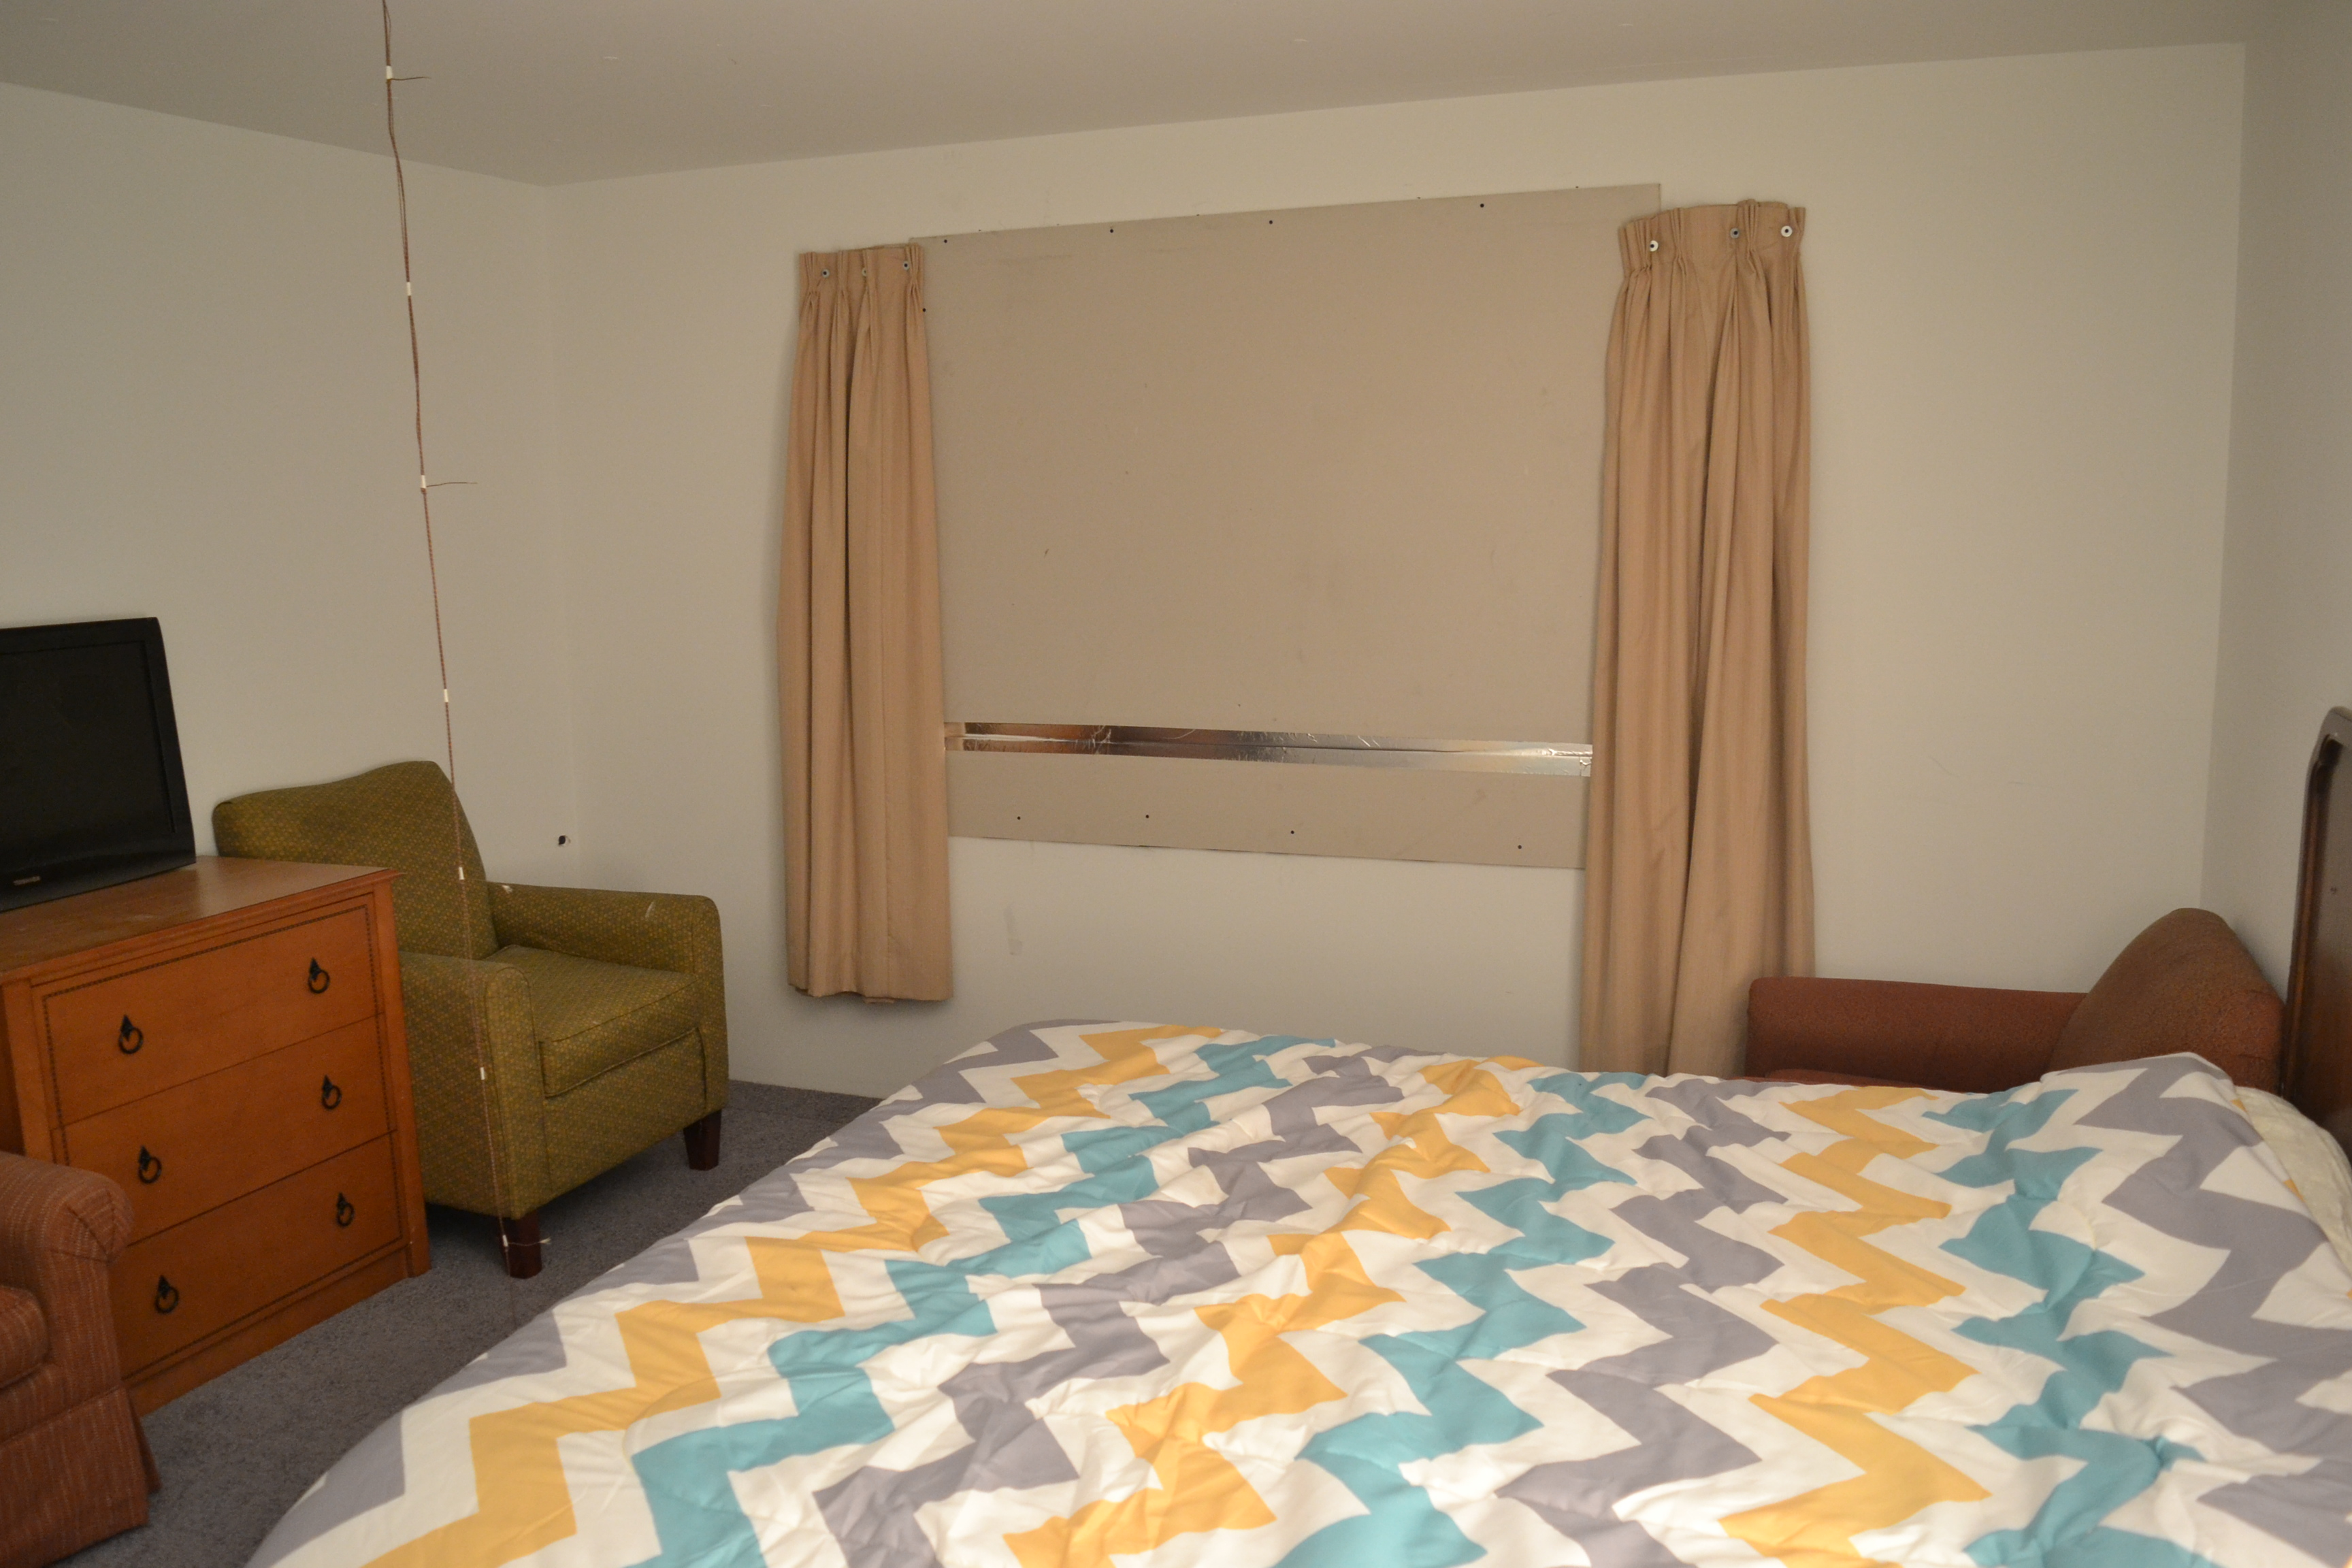
\includegraphics[width=0.50\textwidth]{0_Images/Ranch_Pictures/Exp_3_Fuel.jpg}
\caption{Bedroom 1 Fuel Configuration}
\label{figure:Bed1_fuel}
\end{figure}

\subsection*{Bedroom 2}
Bedroom 1 was furnished to simulate a typical bedroom in a residential home. The fuel load contained 2 stuffed chairs (1 Striped chair and 1 Red Diamond chair), a king-sized bed, dresser, nightstand, pillows, 4'' foam mattress topper, curtains, carpet, and carpet padding. Figure \ref{figure:Bed2_fuel} shows the fuel load for Bedroom 2.

\begin{figure}[H]
\centering
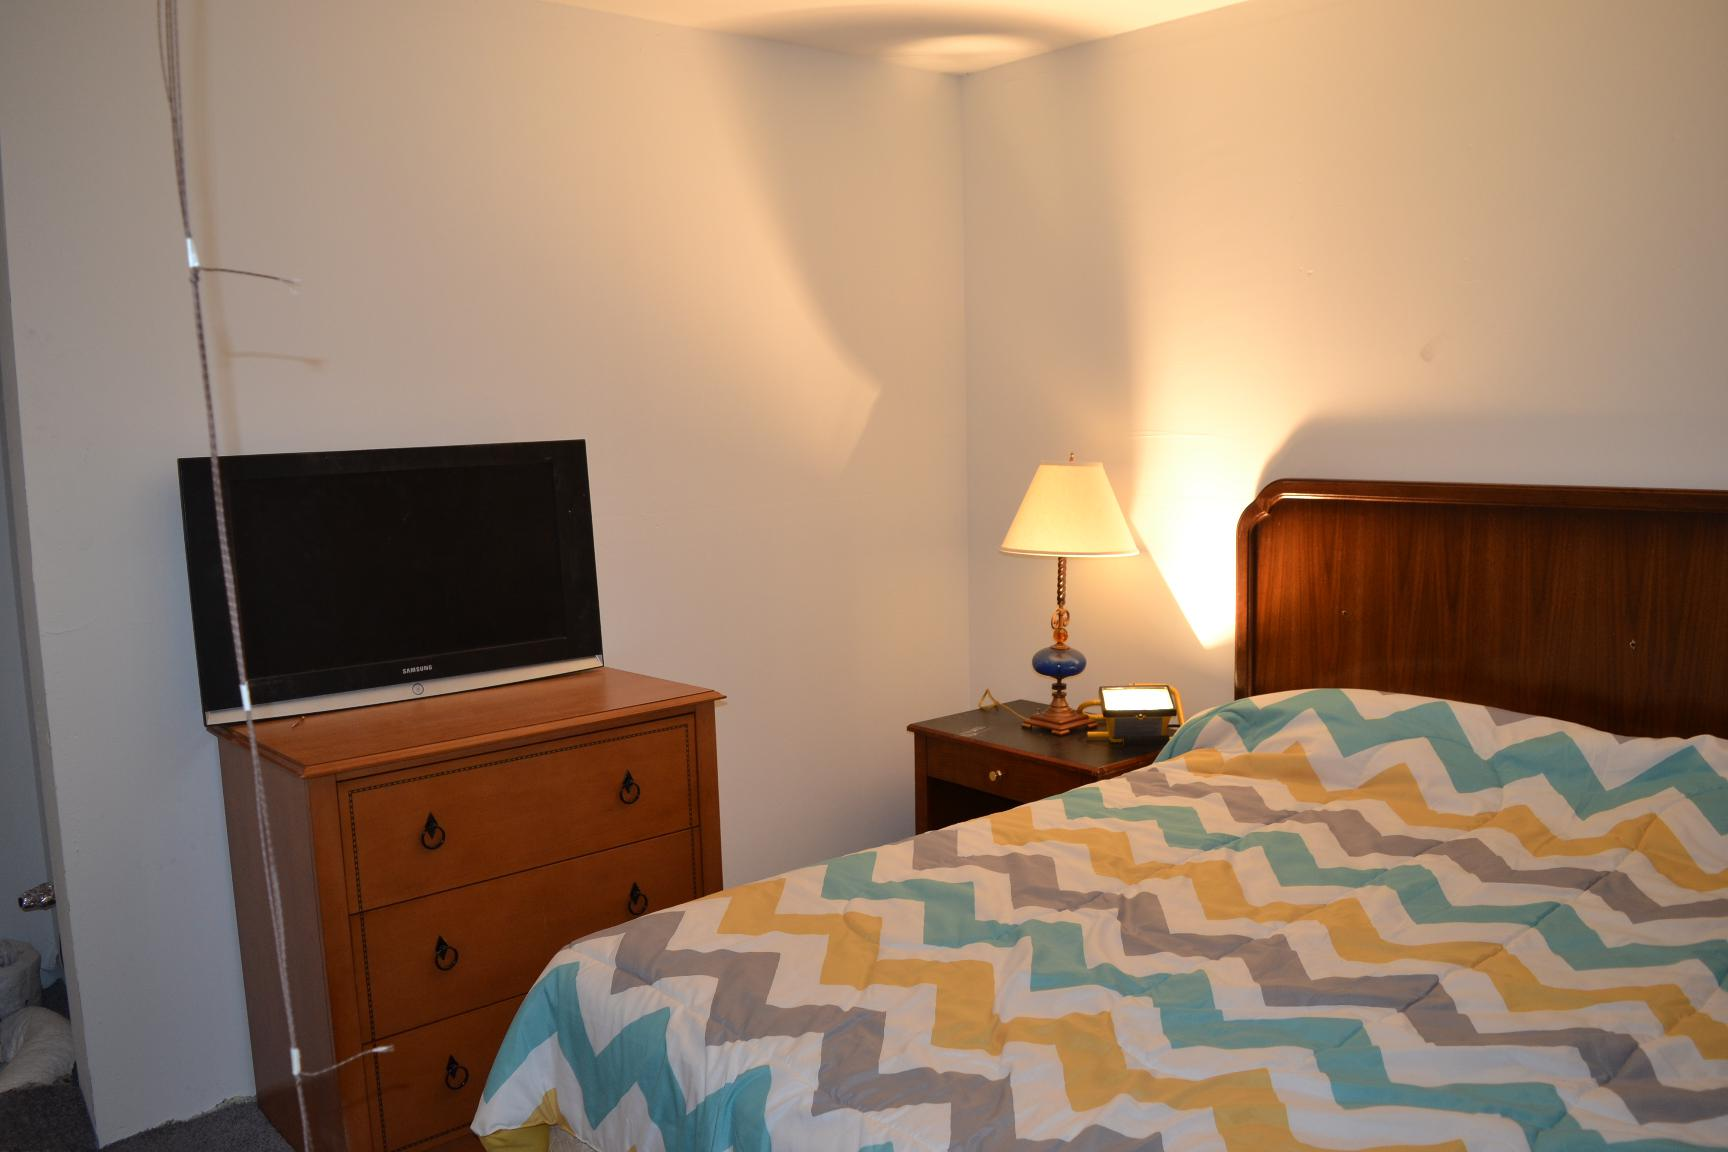
\includegraphics[width=0.45\textwidth]{../0_Images/Fuel/Bedroom_2_1.jpg}
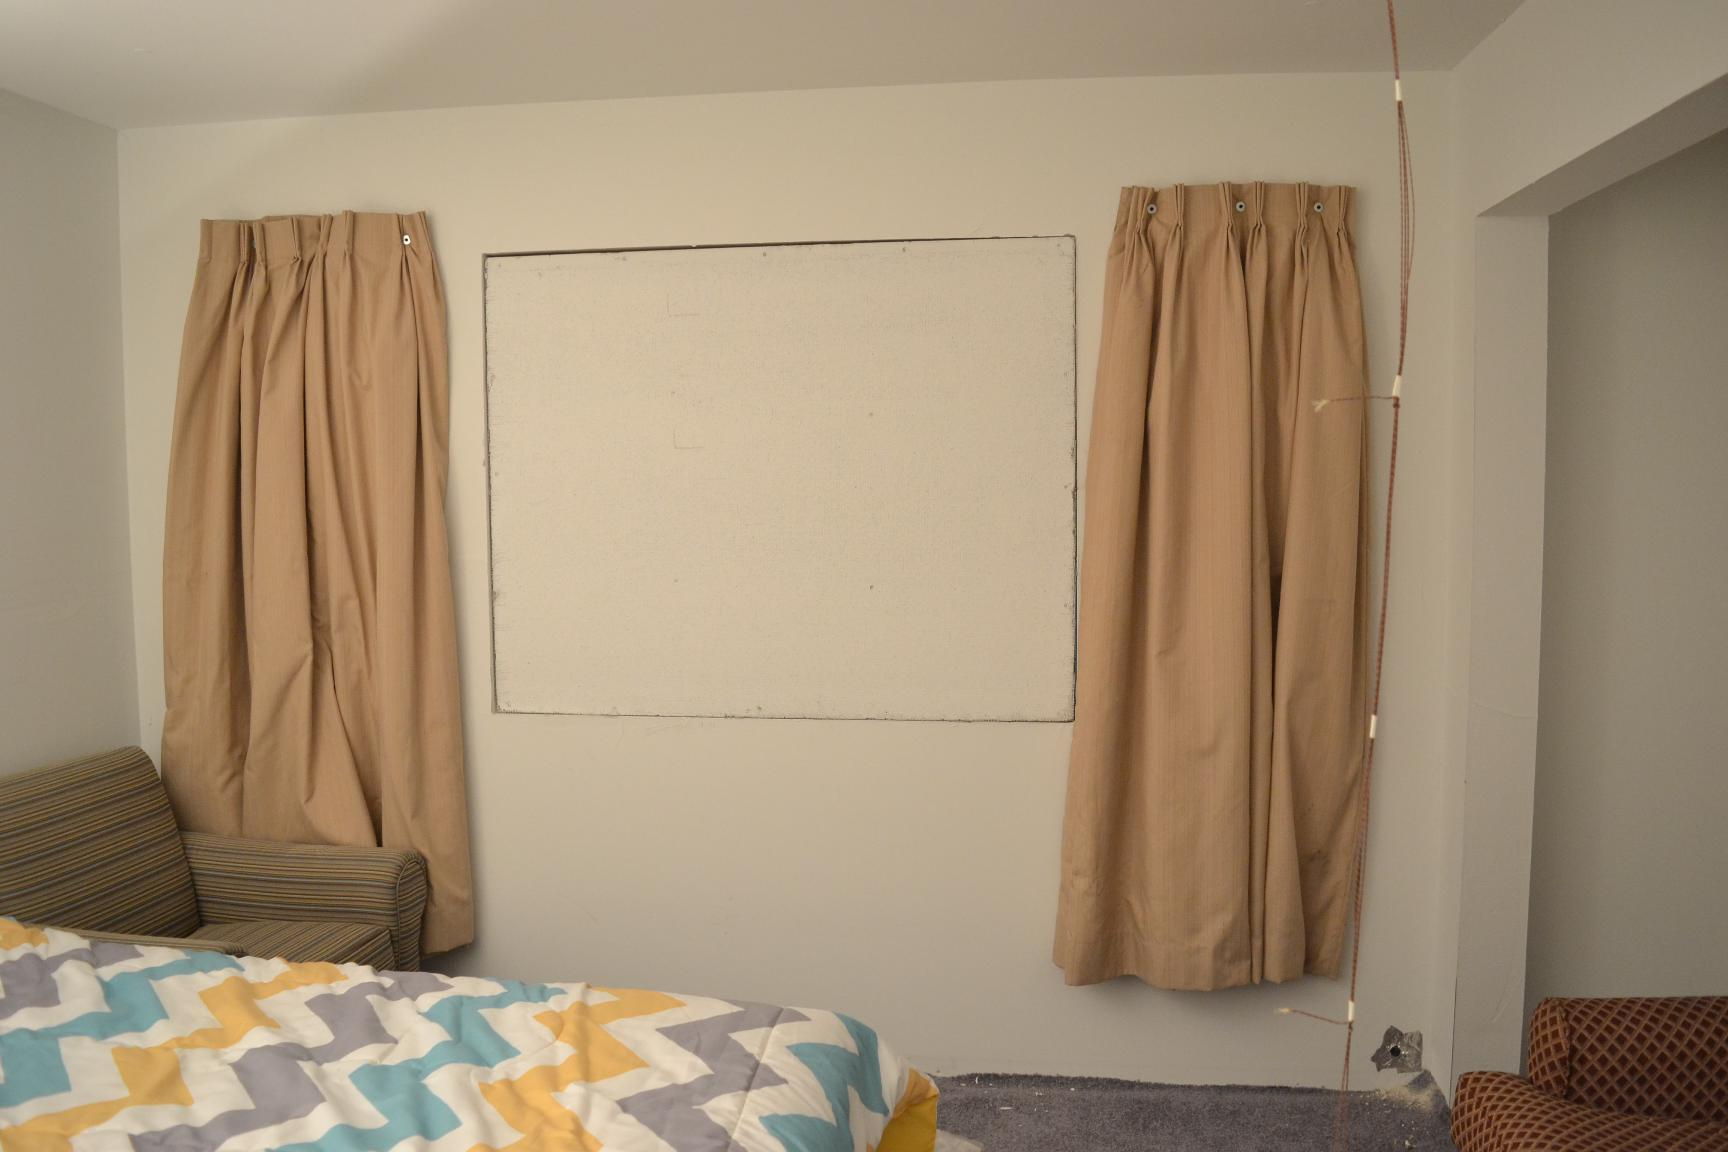
\includegraphics[width=0.45\textwidth]{../0_Images/Fuel/Bedroom_2_2.jpg}
\caption{Bedroom 2 Fuel Configuration}
\label{figure:Bed2_fuel}
\end{figure}

\subsection*{Bedroom 3}
Bedrooms 3 contained 1 stuffed chair (Yellow/Green Chair), a king-sized bed, dresser, nightstand, pillows, 4'' foam mattress topper, curtains, carpet, and carpet padding. Figure \ref{figure:Bed3_fuel} shows the fuel load for Bedroom 3.

\begin{figure}[H]
\centering
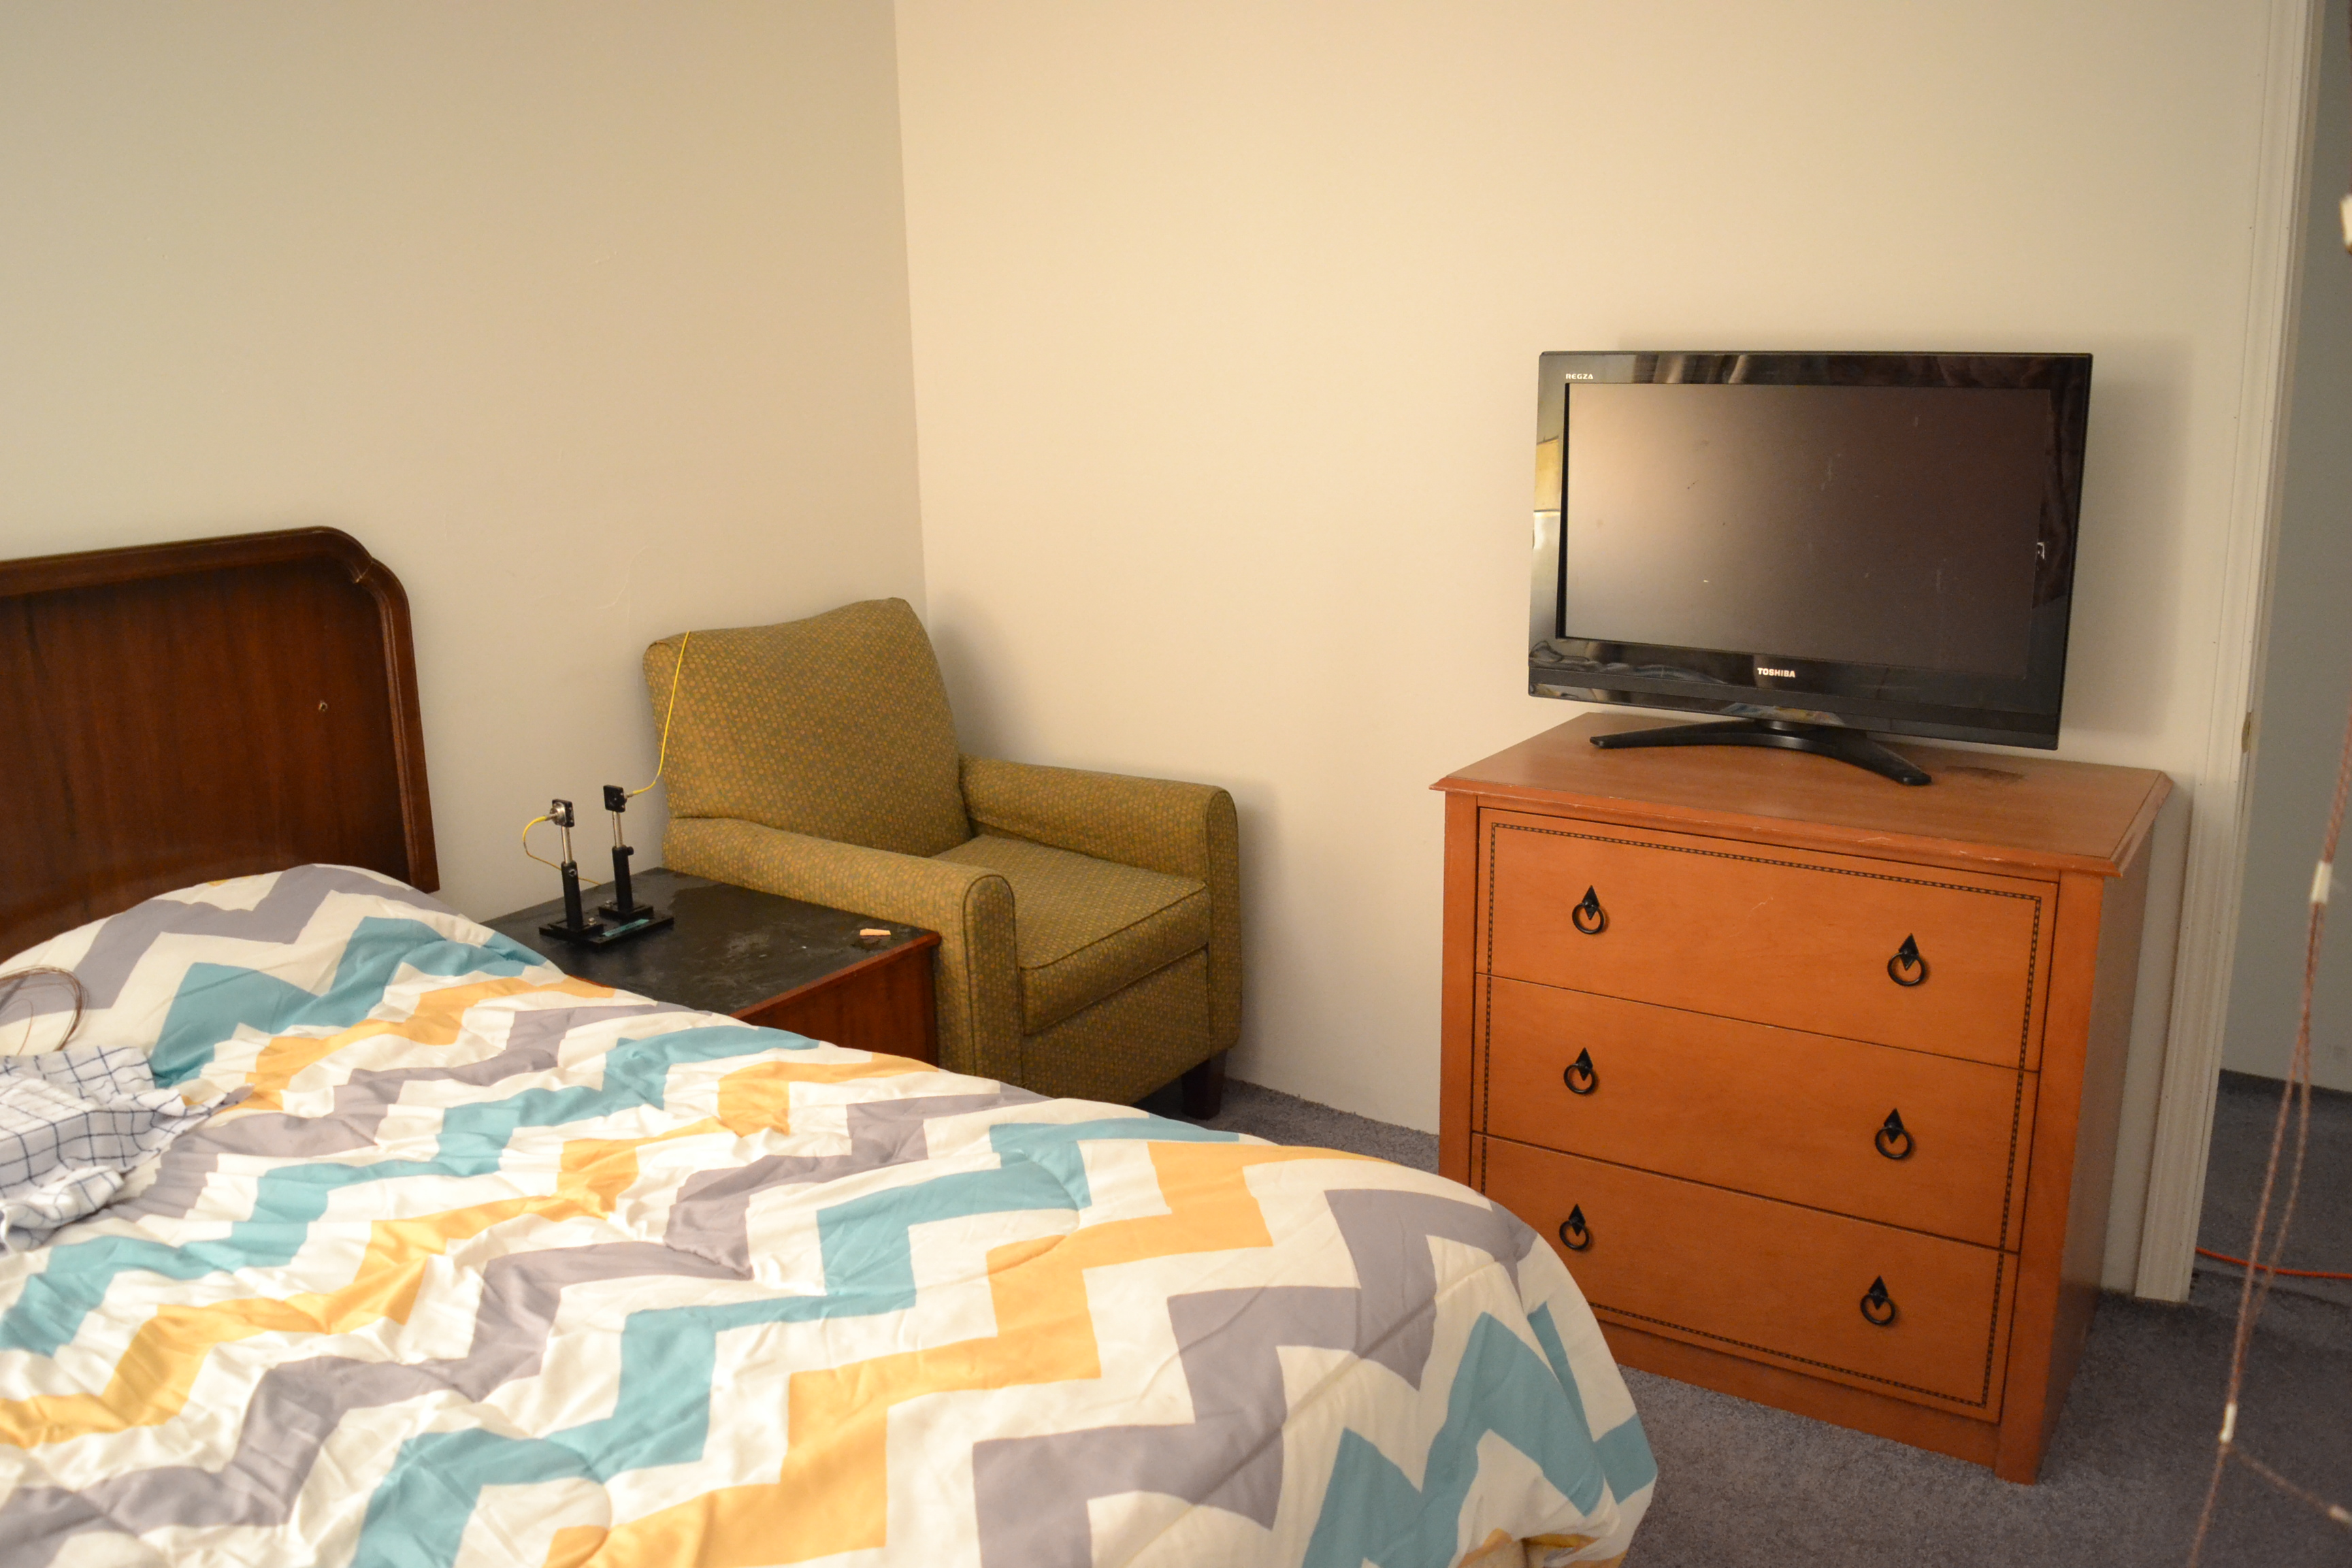
\includegraphics[width=0.45\textwidth]{../0_Images/Fuel/Bedroom_3_1.jpg}
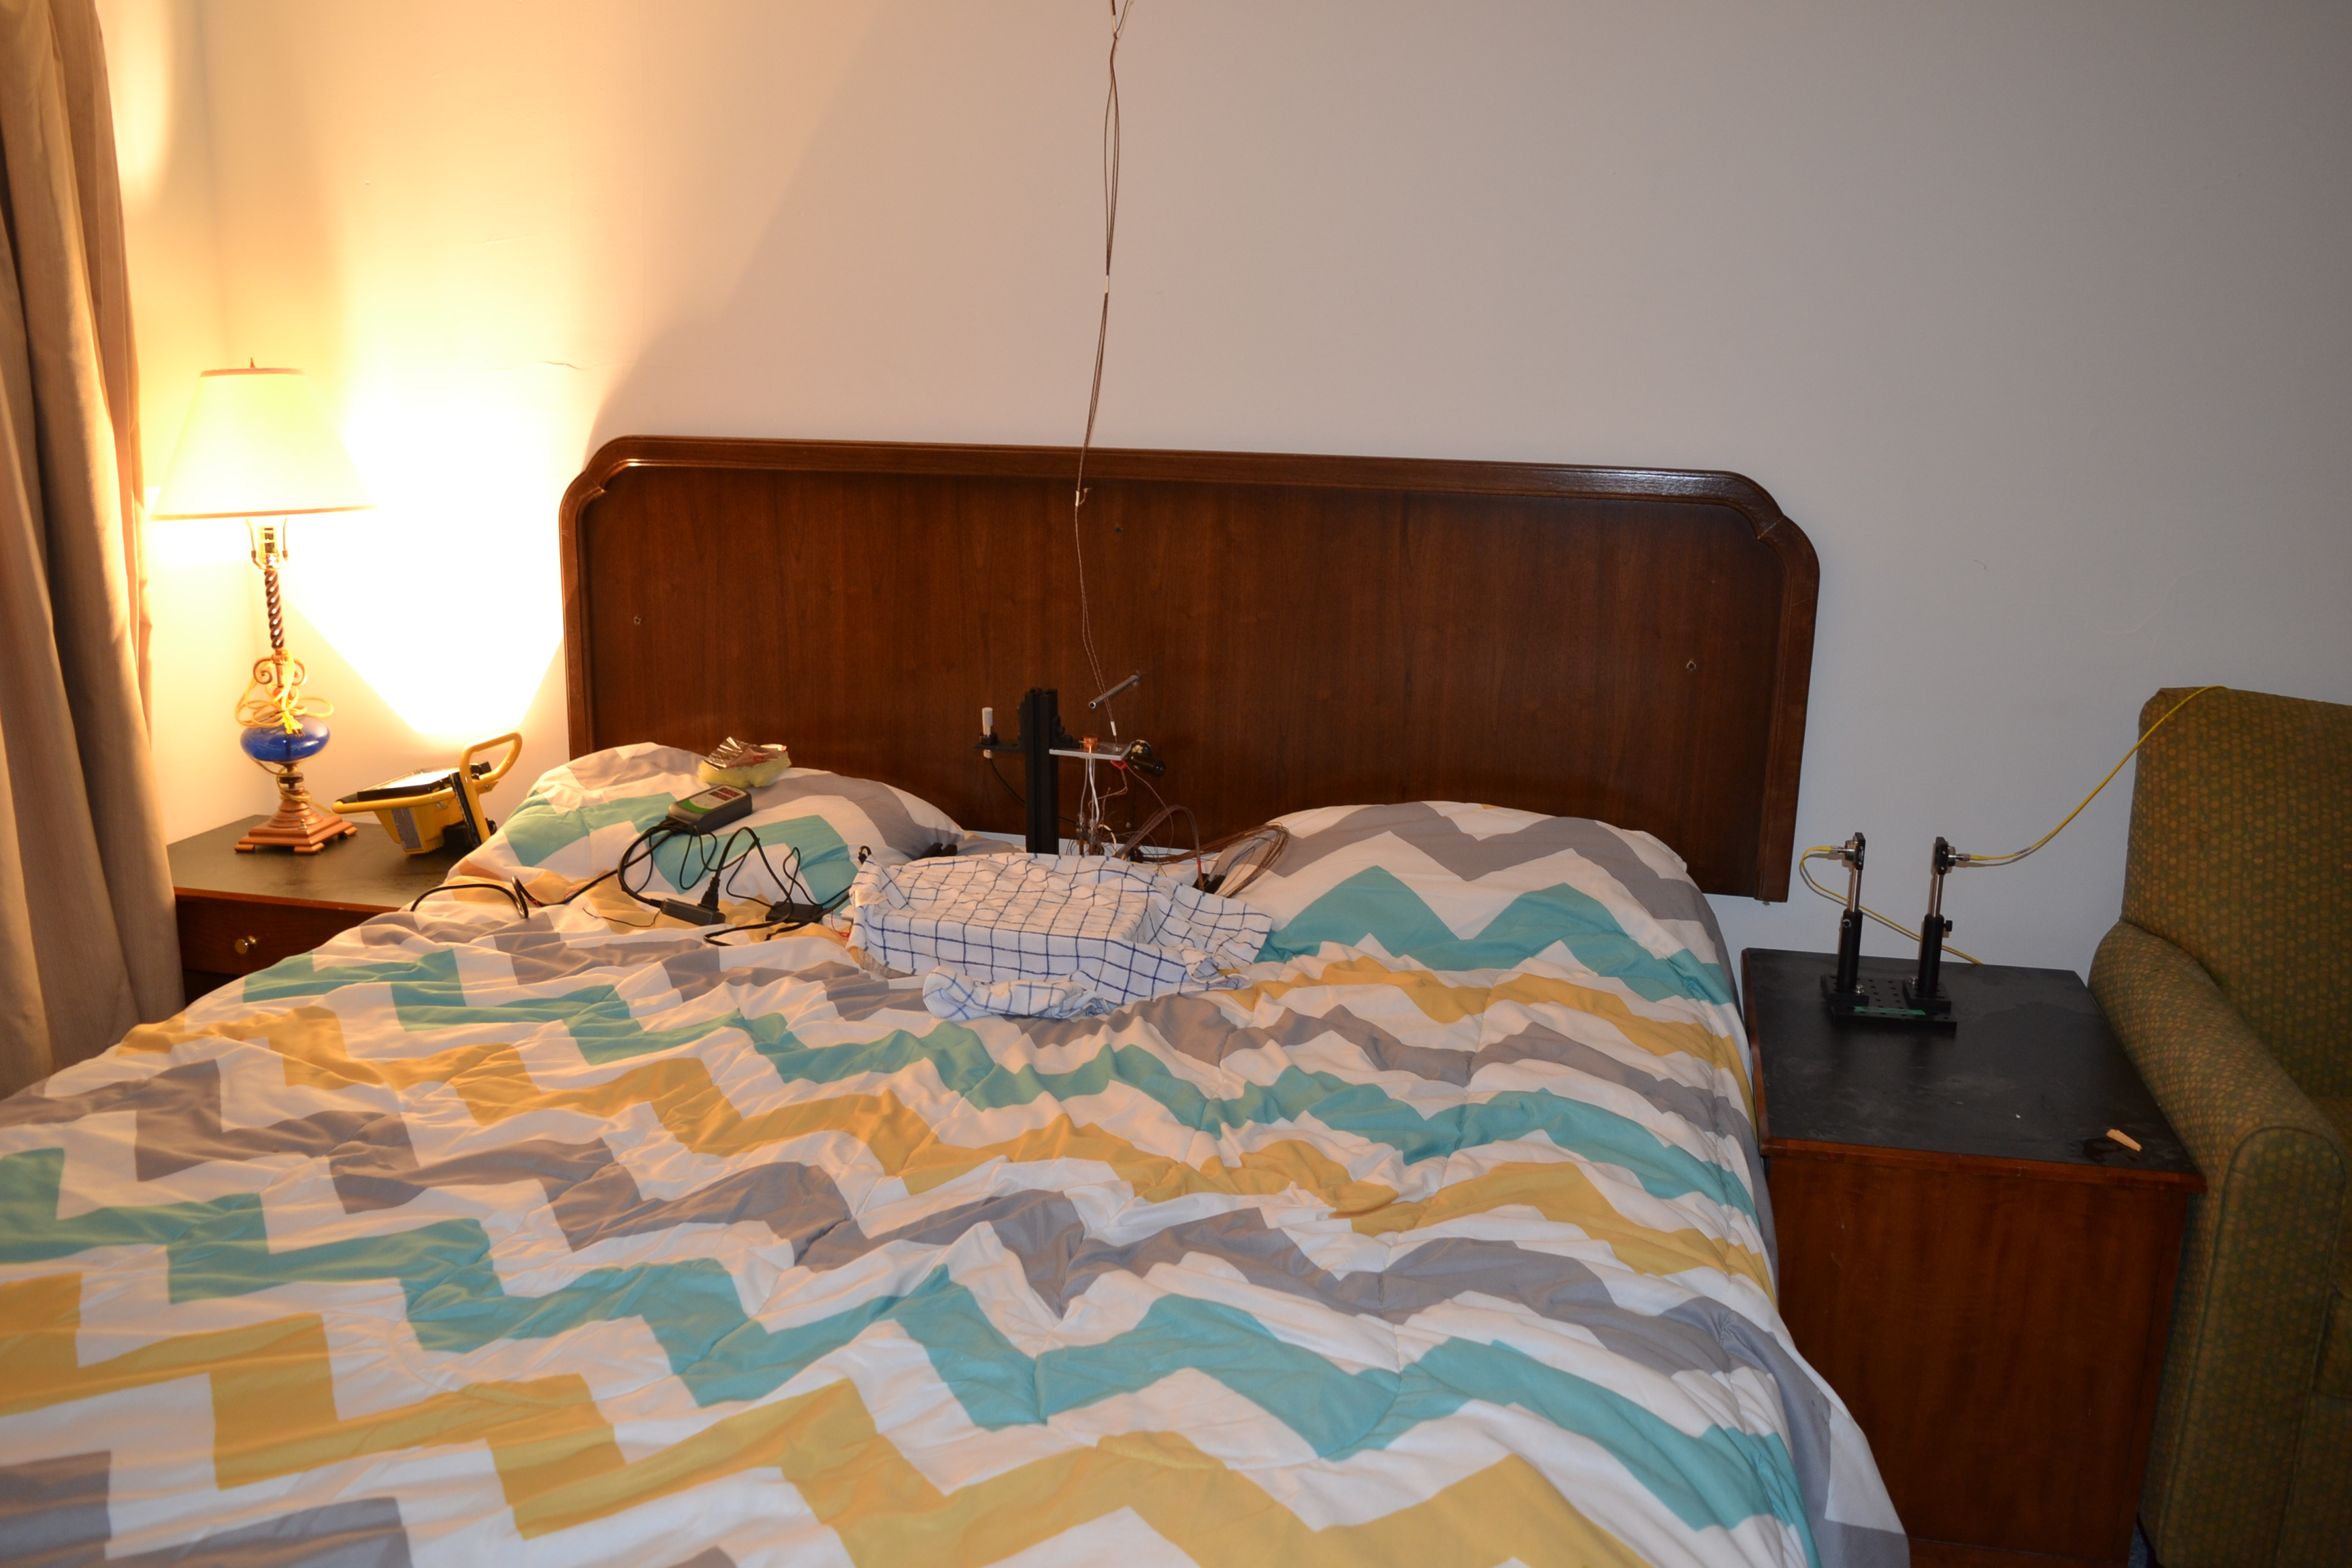
\includegraphics[width=0.45\textwidth]{../0_Images/Fuel/Bedroom_3_2.jpg}
\caption{Bedroom 3 Fuel Configuration}
\label{figure:Bed3_fuel}
\end{figure}

\subsection*{Bedroom 4}
Bedrooms 4 contained 1 stuffed chair (Yellow/Green Chair), a king-sized bed, dresser, nightstand, pillows, 4'' foam mattress topper, curtains, carpet, and carpet padding. Figure \ref{figure:Bed4_fuel} shows the fuel load for Bedroom 4.

\begin{figure}[H]
\centering
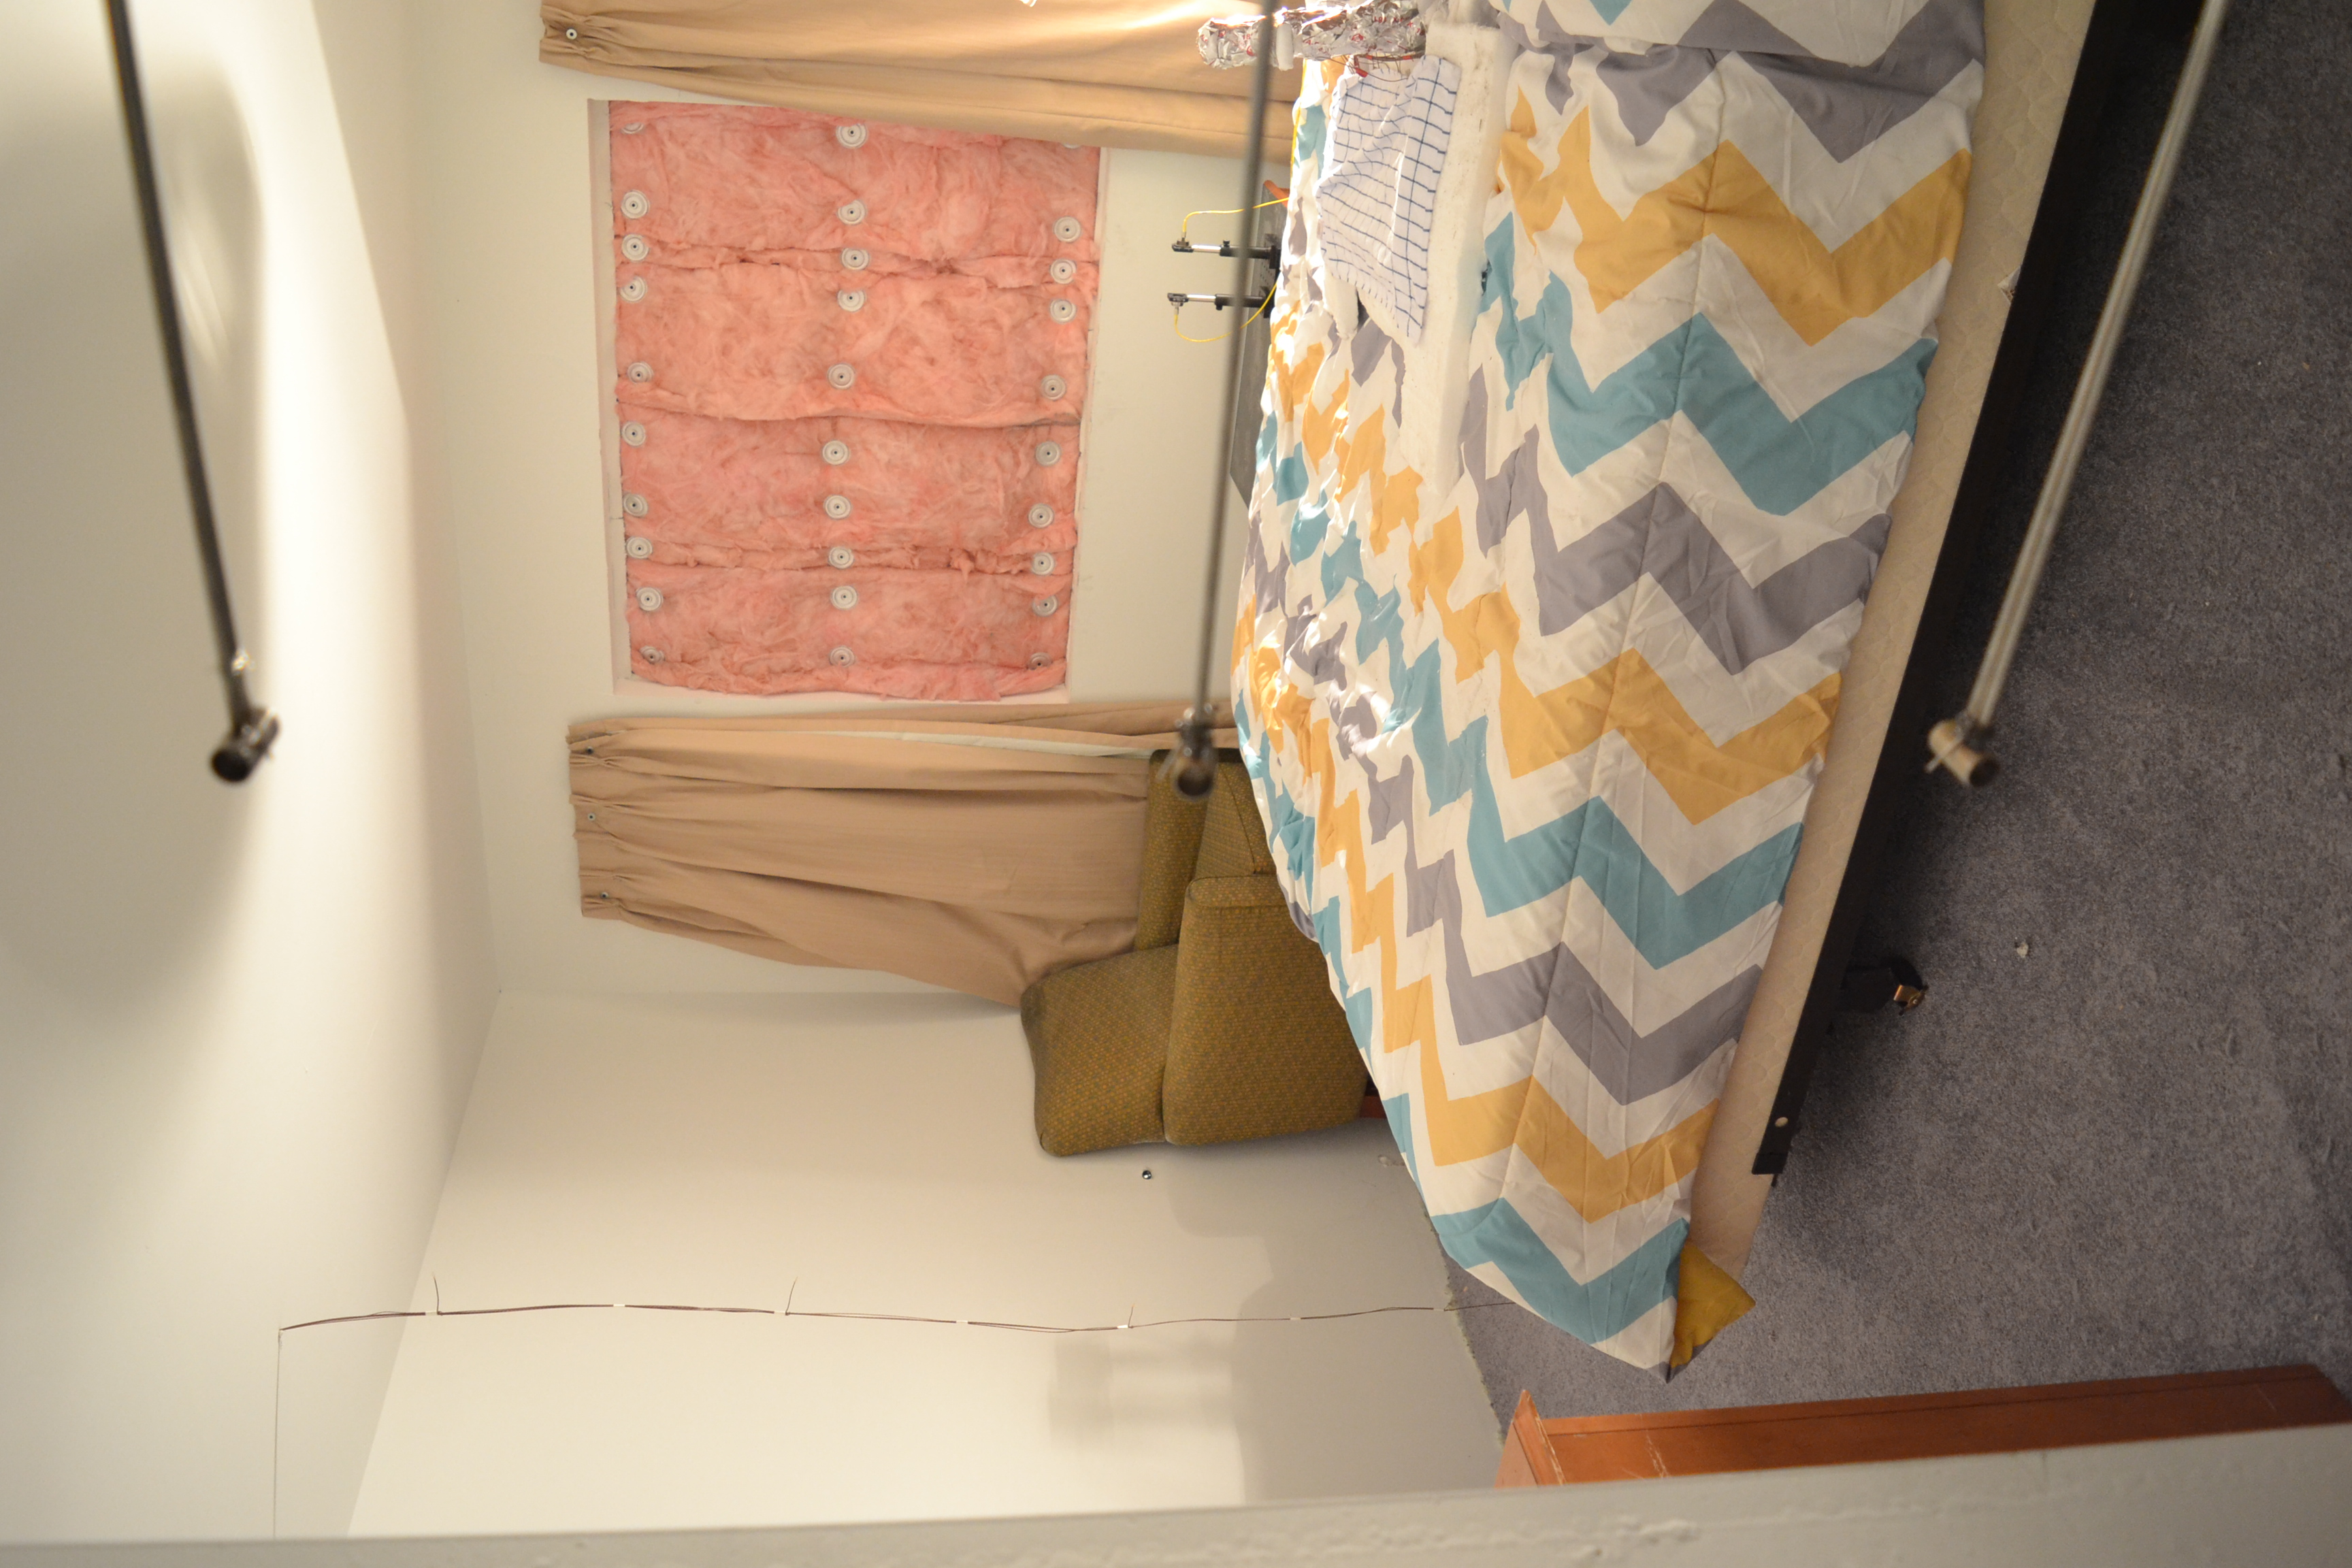
\includegraphics[height=0.40\textwidth]{../0_Images/Fuel/Bedroom_4_1.jpg}
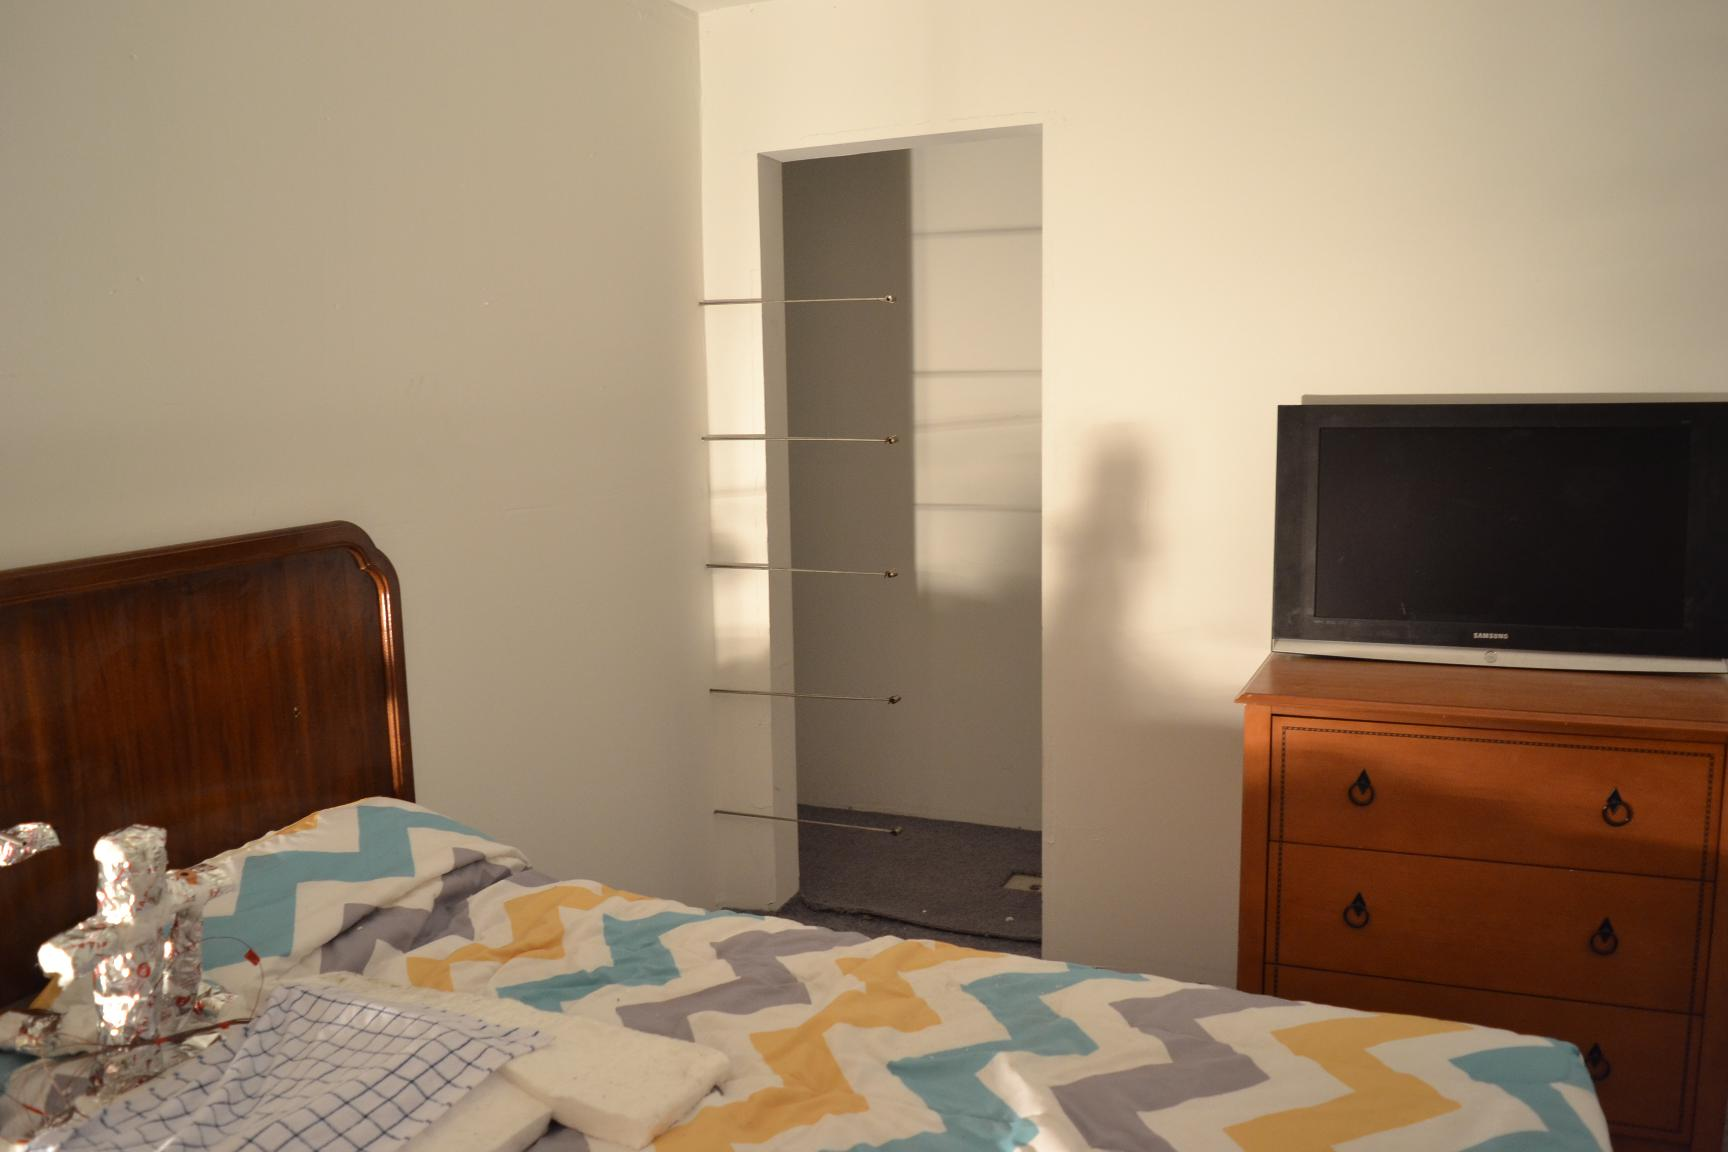
\includegraphics[height=0.40\textwidth]{../0_Images/Fuel/Bedroom_4_2.jpg}
\caption{Bedroom 4 Fuel Configuration}
\label{figure:Bed4_fuel}
\end{figure}

\clearpage

\subsection*{Kitchen}
The kitchen contained a kitchen table and 6 chairs. Figure \ref{figure:Kitchen_fuel} shows the fuel load in the Kitchen. 

\begin{figure}[H]
\centering
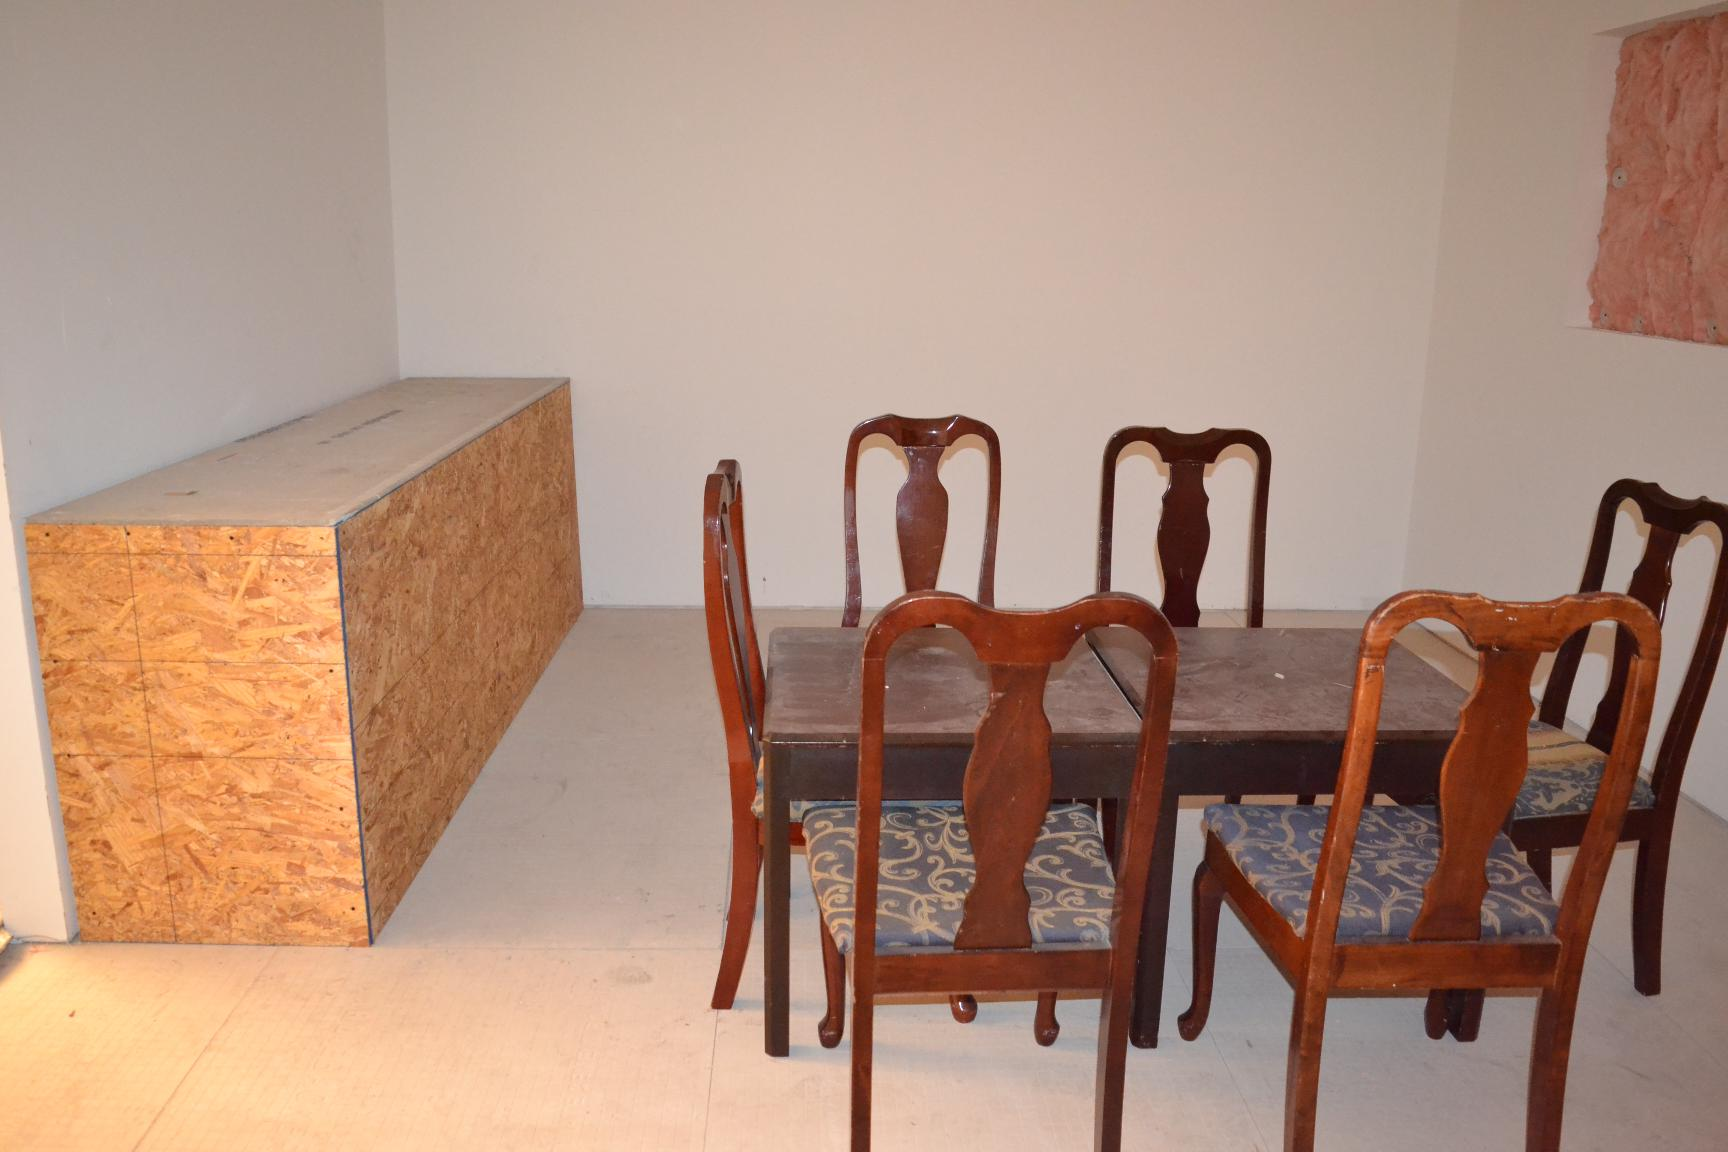
\includegraphics[width=0.45\textwidth]{../0_Images/Fuel/Kitchen.jpg}
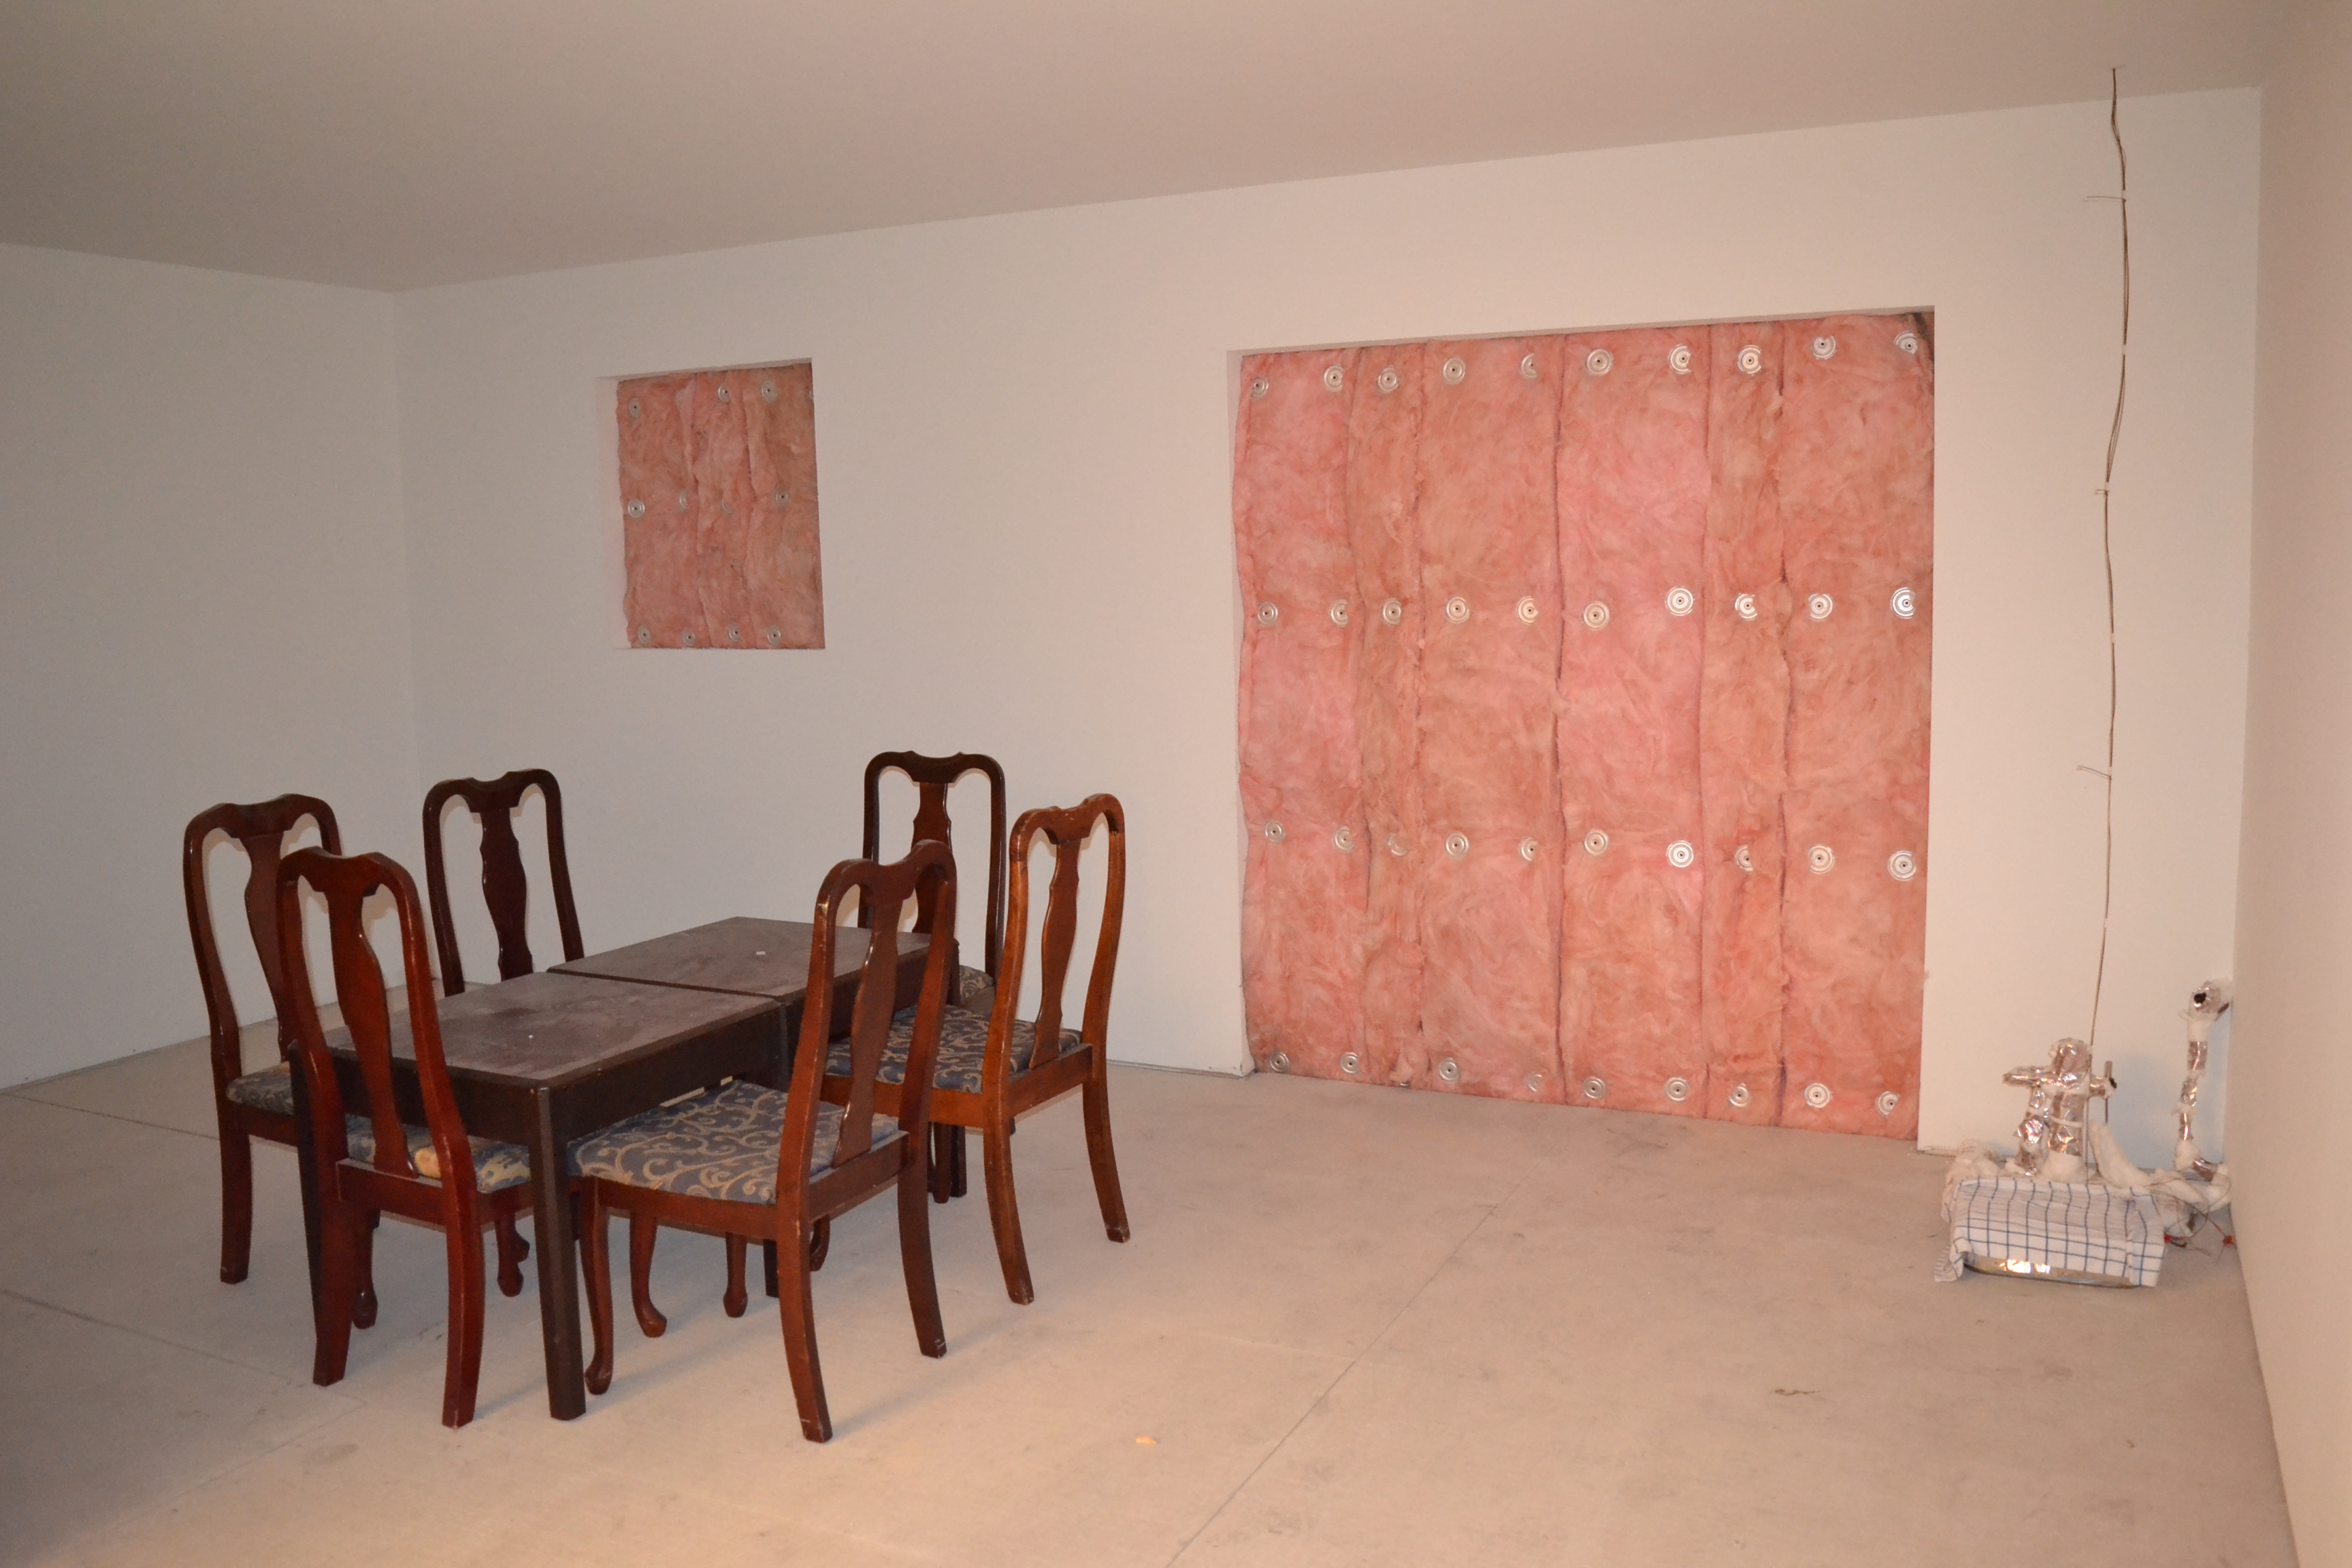
\includegraphics[width=0.45\textwidth]{../0_Images/Fuel/Dining_Room.jpg}
\caption{Kitchen Fuel Configuration}
\label{figure:Kitchen_fuel}
\end{figure}


\subsection*{Living Room}
The living room contained a bookshelf with shelves lined with a 5" foam mattress topper, 2 sofas, 1 stuffed chair (Yellow/Green chair) 2 ottomans, a coffee table, end table, lamp, TV, TV stand, large curtains, carpet, and carpet padding. Figure \ref{figure:Living_Room_fuel} shows the fuel load for the Living Room. 

\begin{figure}[H]
\centering
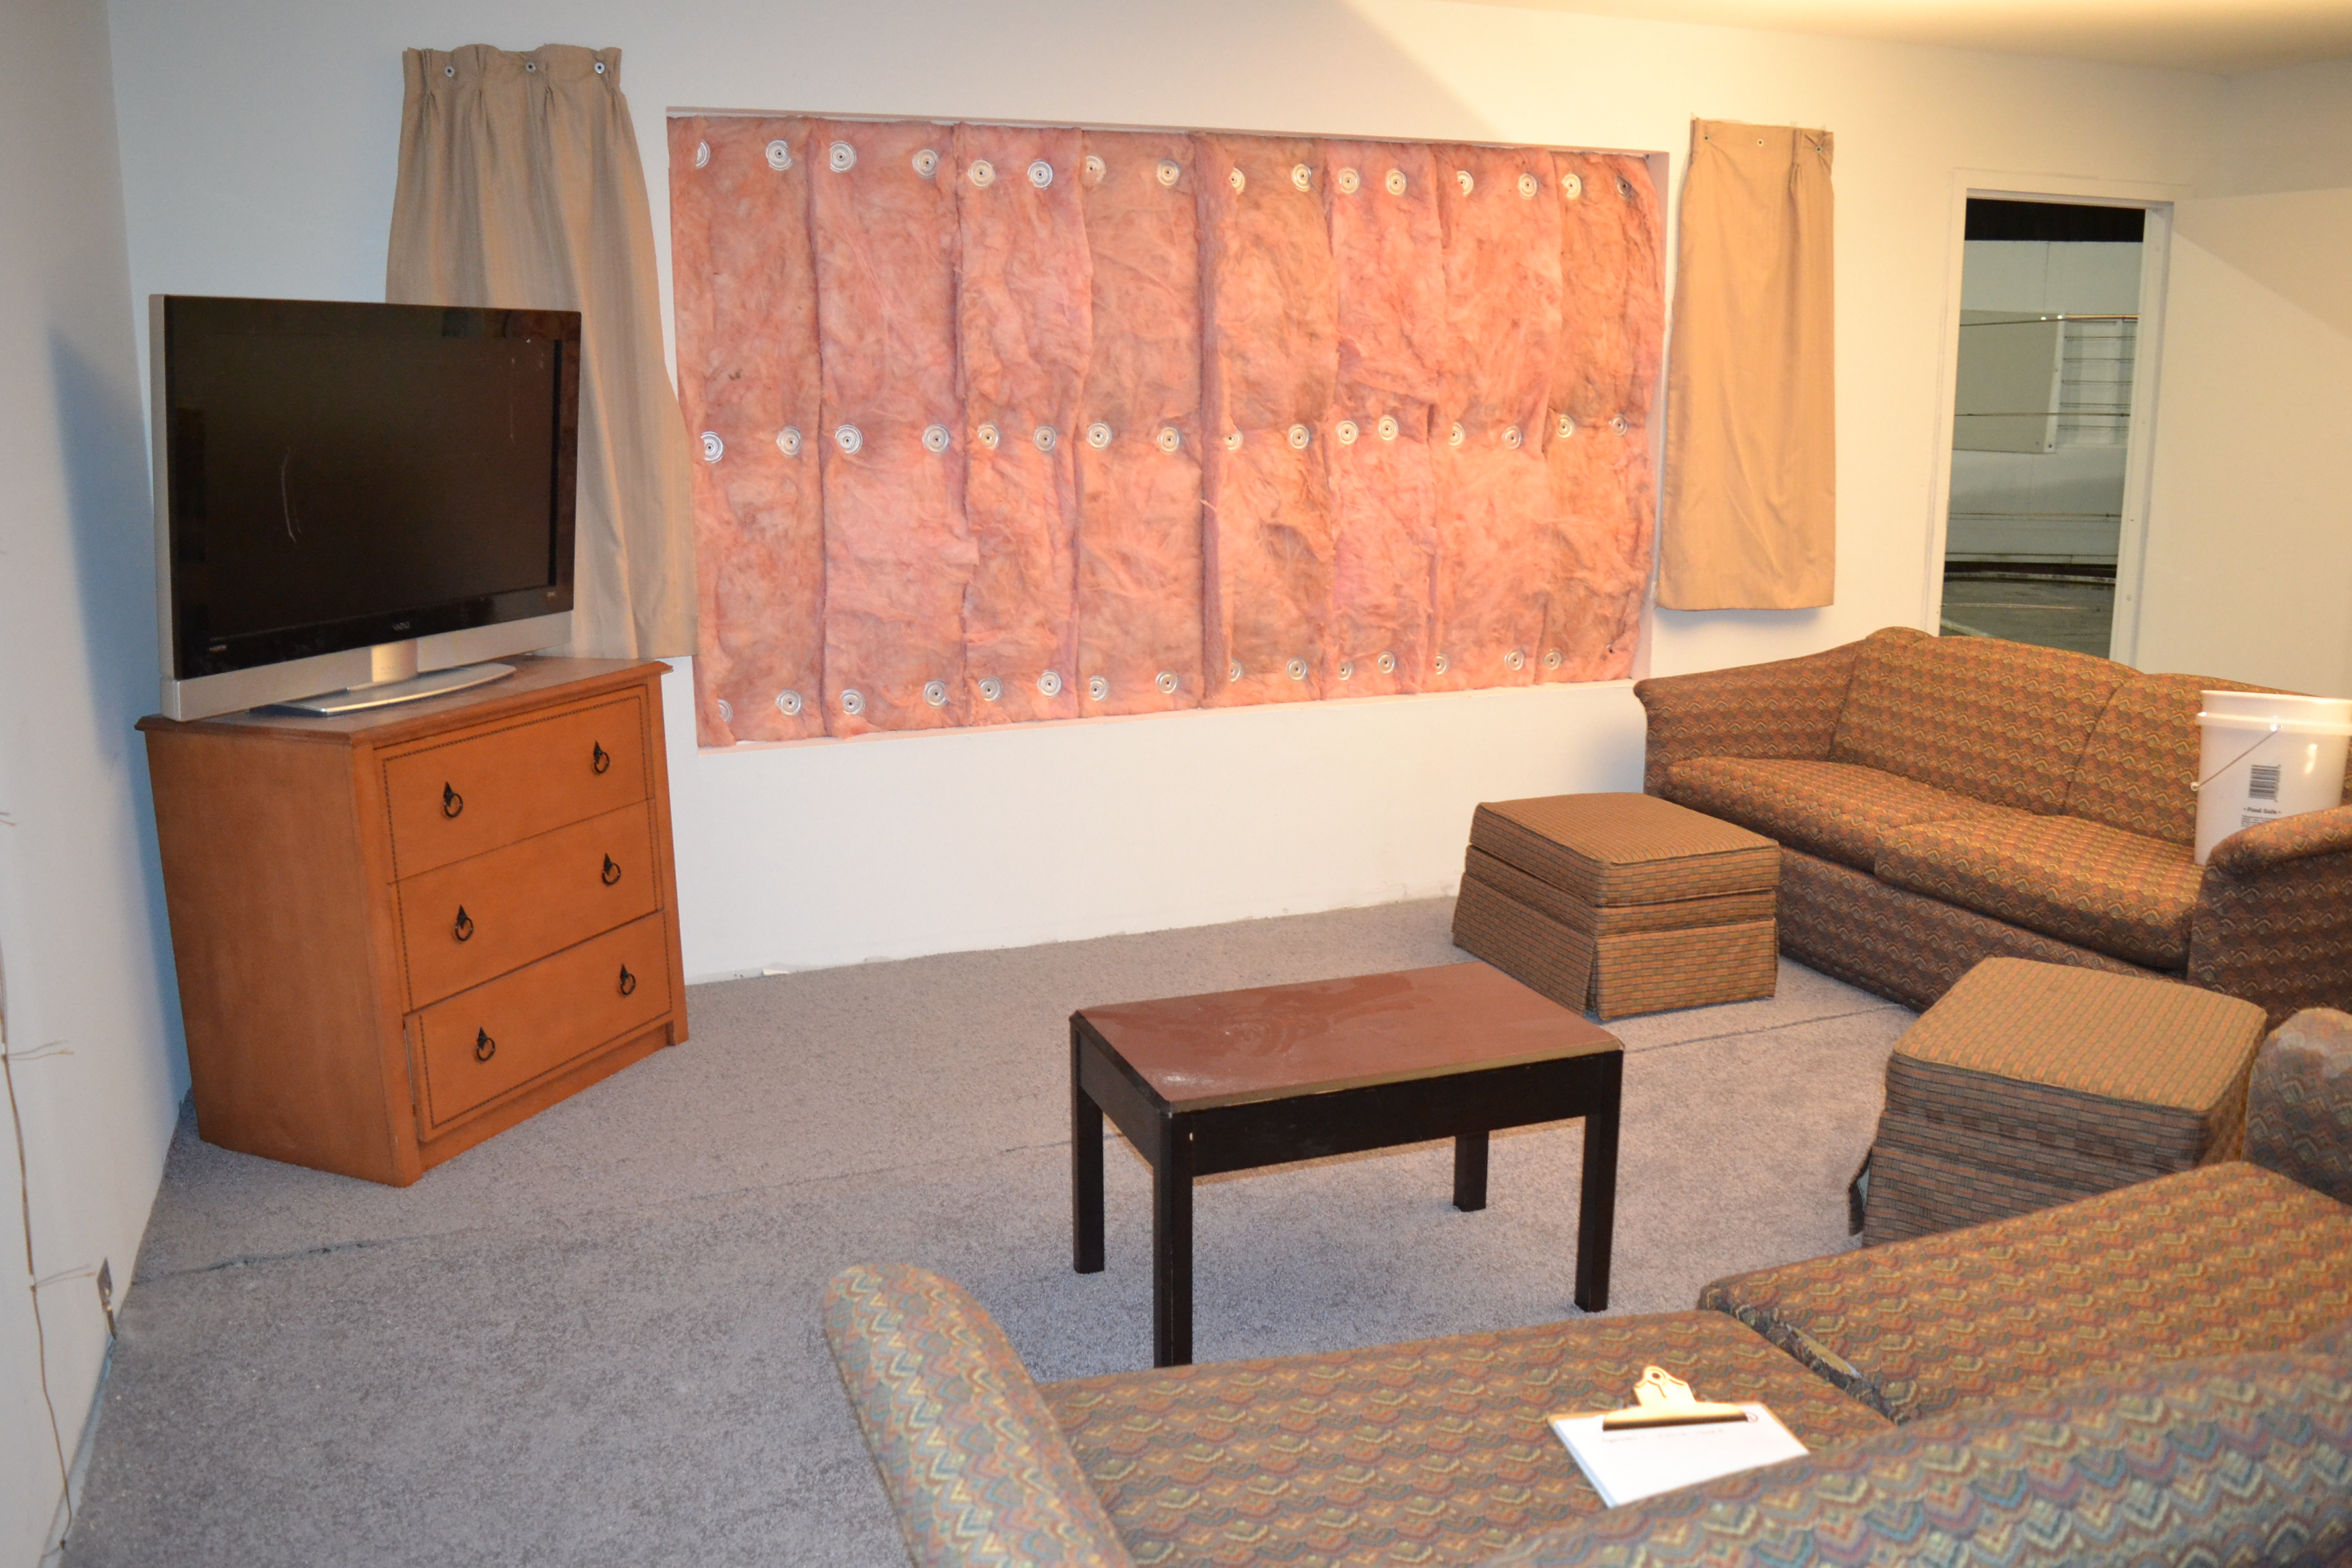
\includegraphics[width=0.45\textwidth]{../0_Images/Fuel/Living_Room.jpg}
\caption{Living Room Fuel Configuration}
\label{figure:Living_Room_fuel}
\end{figure}

\clearpage

\section{Environment Measurement Instrumentation}

Measurements of temperature, heat flux, pressure, and gas velocity were taken at various locations. The same instrumentation was used throughout the duration of the study. The following describes the instrumentation used and uncertainty.

Heat flux measurements were made using a 2.54~cm nominal diameter water-cooled Schmidt- Boelter heat flux gauge (Figure \ref{fig:HeatFluxGauge}). The gauges measured the combined radiative and convective heat flux. For these experiments, the dominant form of heat flux is radiative due to the distance of the heat flux gauges from the flames. It should be noted that the convective contribution to the heat flux is dependent upon the surface temperature of the heat flux gauge. The manufacturer gives an uncertainty of $\pm$3\% and results from a study on heat flux calibration found the typical expanded uncertainty to be $\pm$8\% \cite{HeatFluxRoundRobin}.

\begin{figure} [H]
	\centering
	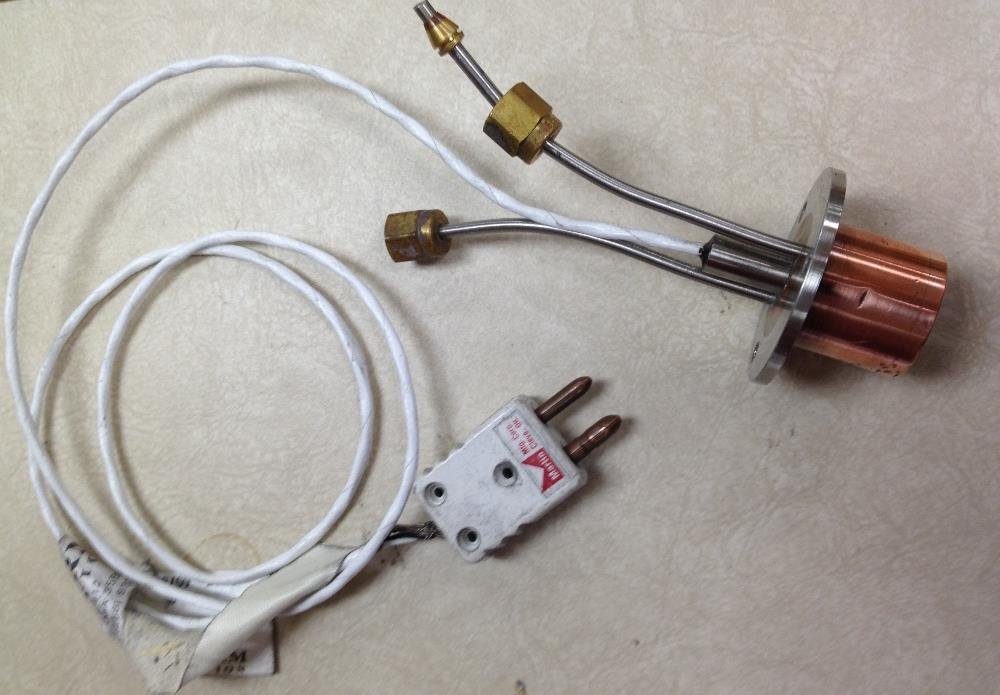
\includegraphics[width = 3.5in]{0_Images/Instrumentation/Heat_Flux_Gauge.jpg}
	\caption{Water Cooled Schmidt-Boelter Heat Flux Gauge}
	\label{fig:HeatFluxGauge}
\end{figure}

Temperatures were recorded using a bare-bead, Chromel-Alumel (Type K) thermocouple with a 0.5 mm nominal diameter (Figure \ref{fig:Thermocouple}). The uncertainty given by the manufacturer for the temperature measurements is $\pm$2.2~$^\circ$C for temperatures below 293~$^\circ$C (560~$^\circ$F)and $\pm$0.75~\% for higher temperatures \cite{TemperatureHandbook}. The thermocouple readings will be lower than the air temperature when the thermocouple is in the flame region, due to radiative losses to the surrounding cooler environment. When the thermocouples are farther from the flame region, the impact of radiation will result in temperature readings higher than the air temperature. Due to the effect of radiative heat transfer to the thermocouples, the expanded uncertainty is approximately $\pm$15~\%.

\begin{figure} [H]
	\centering
	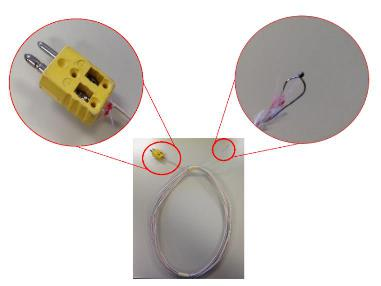
\includegraphics[width = 4in]{0_Images/Instrumentation/Thermocouple.jpg}
	\caption{Chromel-Alumel (Type K) Thermocouple}
	\label{fig:Thermocouple}
\end{figure}

To determine the gas velocity, an array of bi-directional probes was utilized in conjunction with differential pressure transducers and inconel thermocouples. The bi-directional probe was constructed of stainless steel and features a `high' side and a `low' side which travel back to a pressure transducer that evaluates the differential pressure from ambient pressure. The inconel shielded thermocouples were placed in-line with the bi-directional probes to ensure that the measurements were recorded at the same location. The inconel shielded thermocouple was a 0.063~in. diameter type KSL inconel 600 sheathed grounded junction with a type K, 24~gauge glass/glass insulation lead. The differential pressure transducer was a Setra Model 264 with a range of $\pm$1.0~in. WC ($\pm$248.8~Pa). The uncertainty given by the manufacturer is 1~\% or 1.2~Pa. The configuration had a velocity range of $\pm$24.2~m/s ($\pm$54~mph). The pressure transducers were configured in groups of 6, contained in a single plastic box with connections for pressure, temperature and power (Figure~\ref{fig:BDP}). Five probes were installed in openings where velocity measurements were taken, centered horizontally in the opening (Figure~\ref{fig:BDP}). Velocity measurement with this configuration was determined to have an estimated expanded uncertainty of $\pm$18~\% \cite{BDPInPoolFires}.

\begin{figure}[H]
	\centering
	\begin{tabular}{c c}
		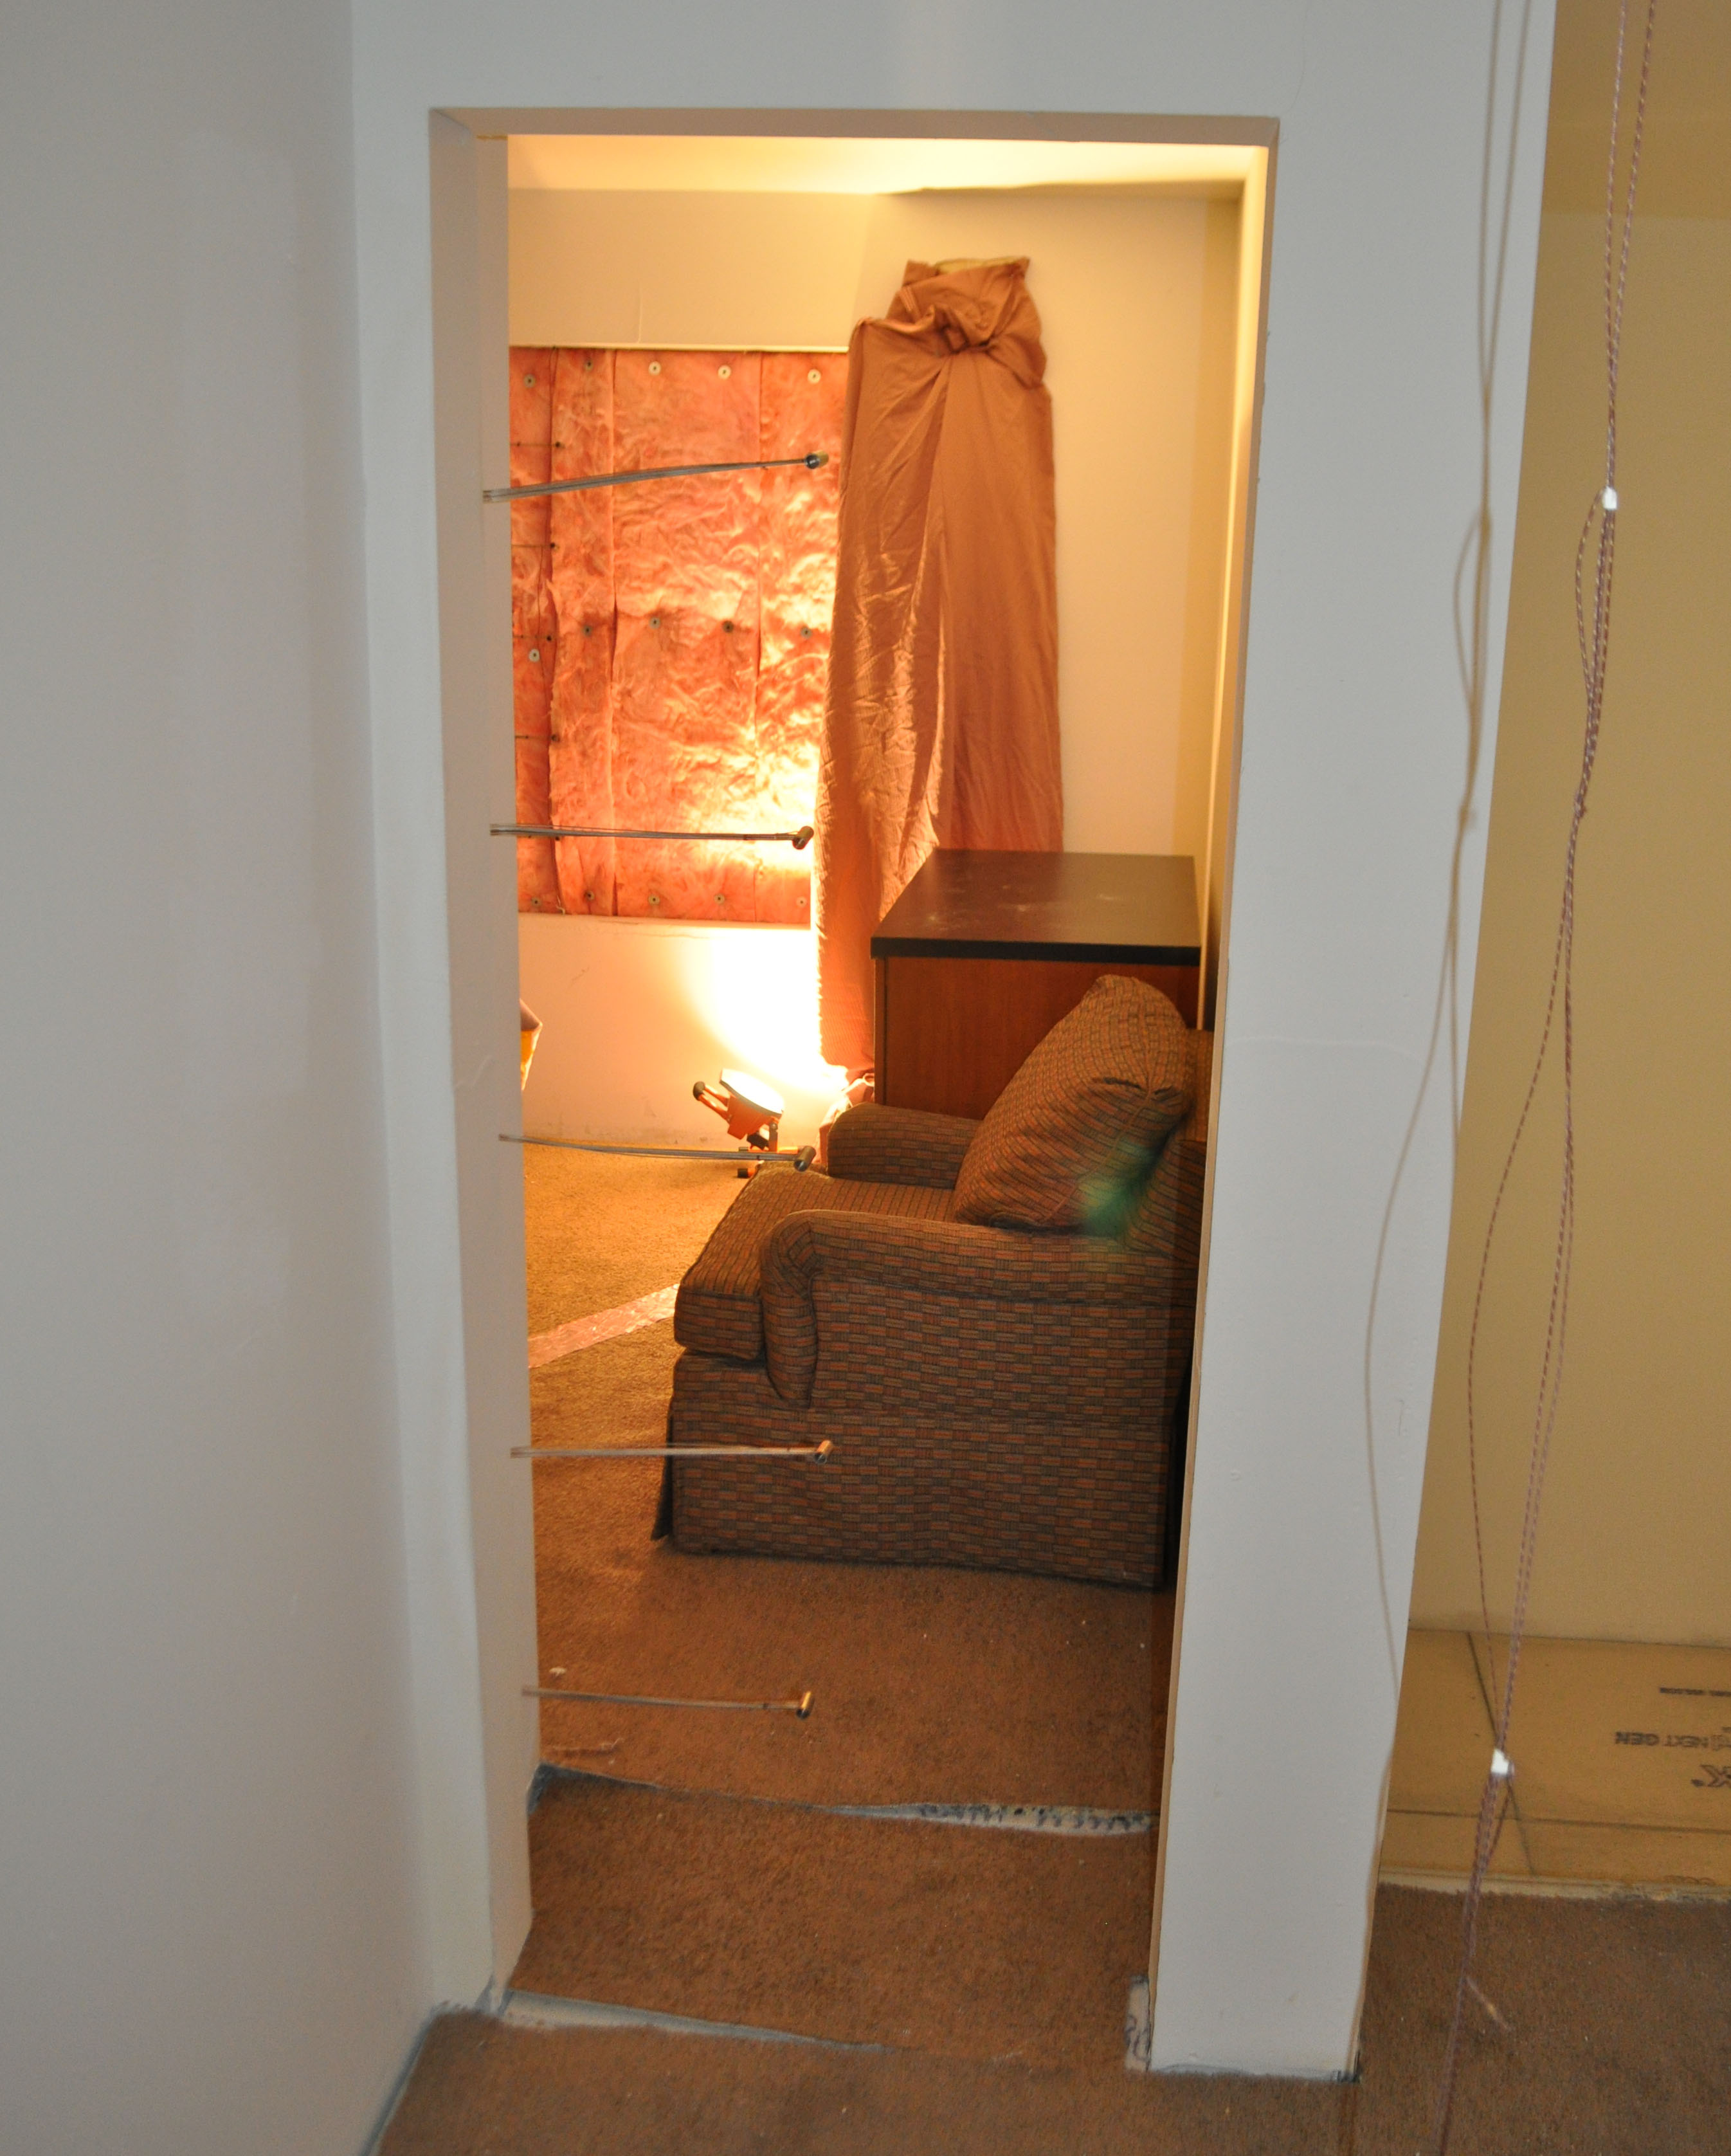
\includegraphics[height = 2.5in]{0_Images/Instrumentation/BDPArray.jpg} &
		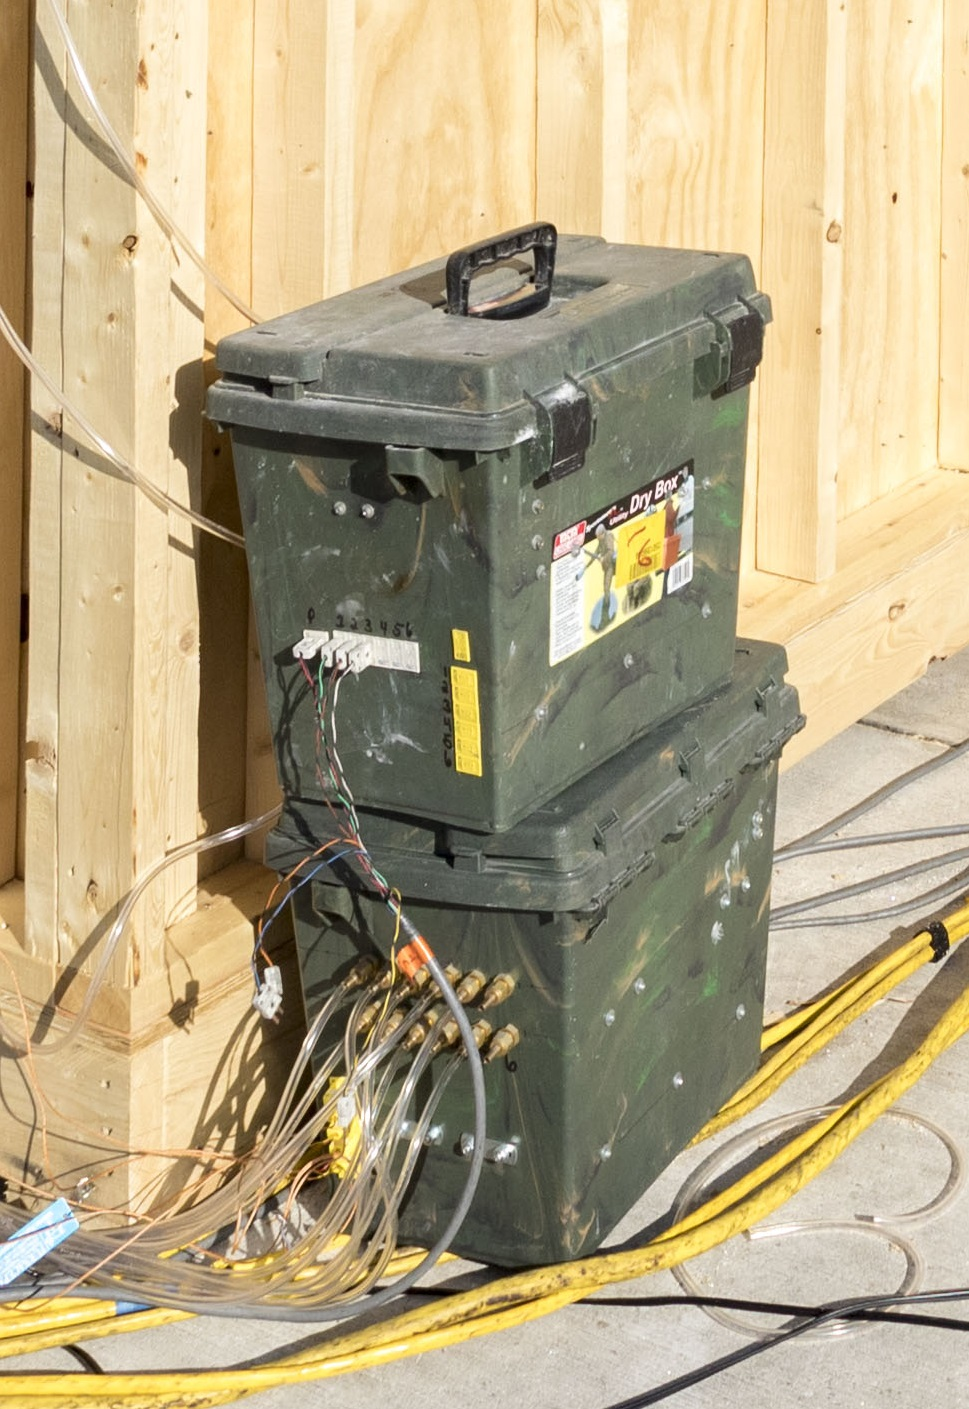
\includegraphics[height = 2.5in]{0_Images/Instrumentation/PressureBox.jpg} \\
	\end{tabular}
	\caption{Bi-Directional Probe Array. Example of probes in a doorway (left), pressure transducer box (right).}
	\label{fig:BDP}
\end{figure}

Standard video was obtained through the use of BoschVTC-206F03-4 video cameras (Figure~\ref{fig:BullettCam}). Thermal imaging of the front and rear of the structure was taken using ISG Infrasys Elite XR (Figure~\ref{fig:IRCam}). The thermal imaging camera has a fixed emissivity value of 0.9 and was utilized for visual representation of relative conditions, no temperature measurements or analysis were derived using the camera. All cameras were recorded Samsung Model SRD-1680 DN digital video recorder set to 24 frames per second with a quality of ``high''.

\begin{figure}[H]
	\centering
	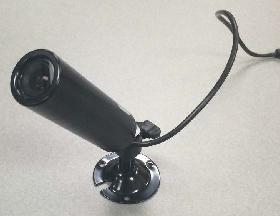
\includegraphics[width = 3in]{0_Images/Instrumentation/BullettCam.jpg}

	\caption{BoschVTC-206F03-4 video camera}
	\label{fig:BullettCam}
\end{figure}

\begin{figure}[H]
	\centering
	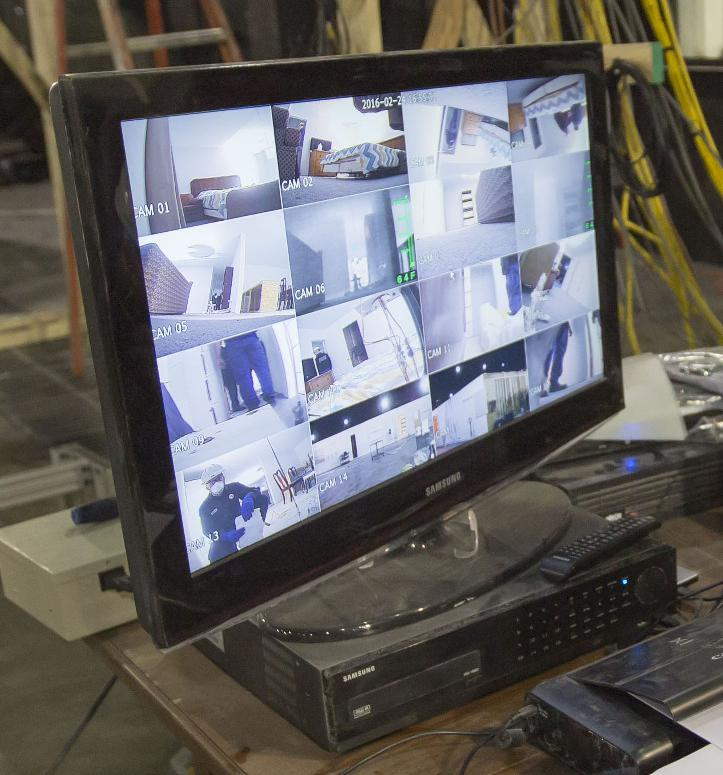
\includegraphics[width = 3in]{0_Images/Instrumentation/DVR.jpg}

	\caption{Samsung Model SRD-1680 DN Digital Video Recorder with Monitor}
	\label{fig:DVR}
\end{figure}

\begin{figure}[H]
	\centering
	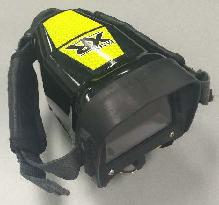
\includegraphics[height = 2.5in]{0_Images/Instrumentation/ISG_IR.jpg}
	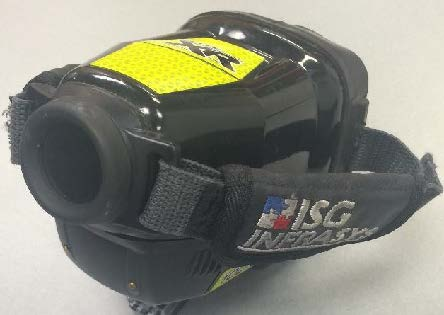
\includegraphics[height = 2.5in]{0_Images/Instrumentation/ISG_IR2.jpg}
	\caption{ISG Elite XR Fire Service Thermal Imaging Camera}
	\label{fig:IRCam}
\end{figure}

Gas samples were analyzed through the use of OxyMat6 and UltraMat23 Siemens gas analyzers. Samples were pulled from the structure through the use of Cole Palmer Model L-79200-30 vacuum/pressure diaphragm pump rated at 0.75~CFM via a stainless steel tube. The sample is filtered through a course filter, Solberg Model 842, 2 micron paper filter before running through a condensing trap to remove moisture. The sample then runs through a drying tube dry fine filter, Perma Pure Model FF-250-SG-2.5G with a 1 micron filter FF-250-E-2.5G before splitting into two branches and entering the UltraMat and OxyMat analyzer. The analyzers are calibrated to measure CO from 0-50000~PPM, CO$_2$ from 0-20~\% and O$_2$ from 0-25~\%. 

\begin{figure}[H]
	\centering
	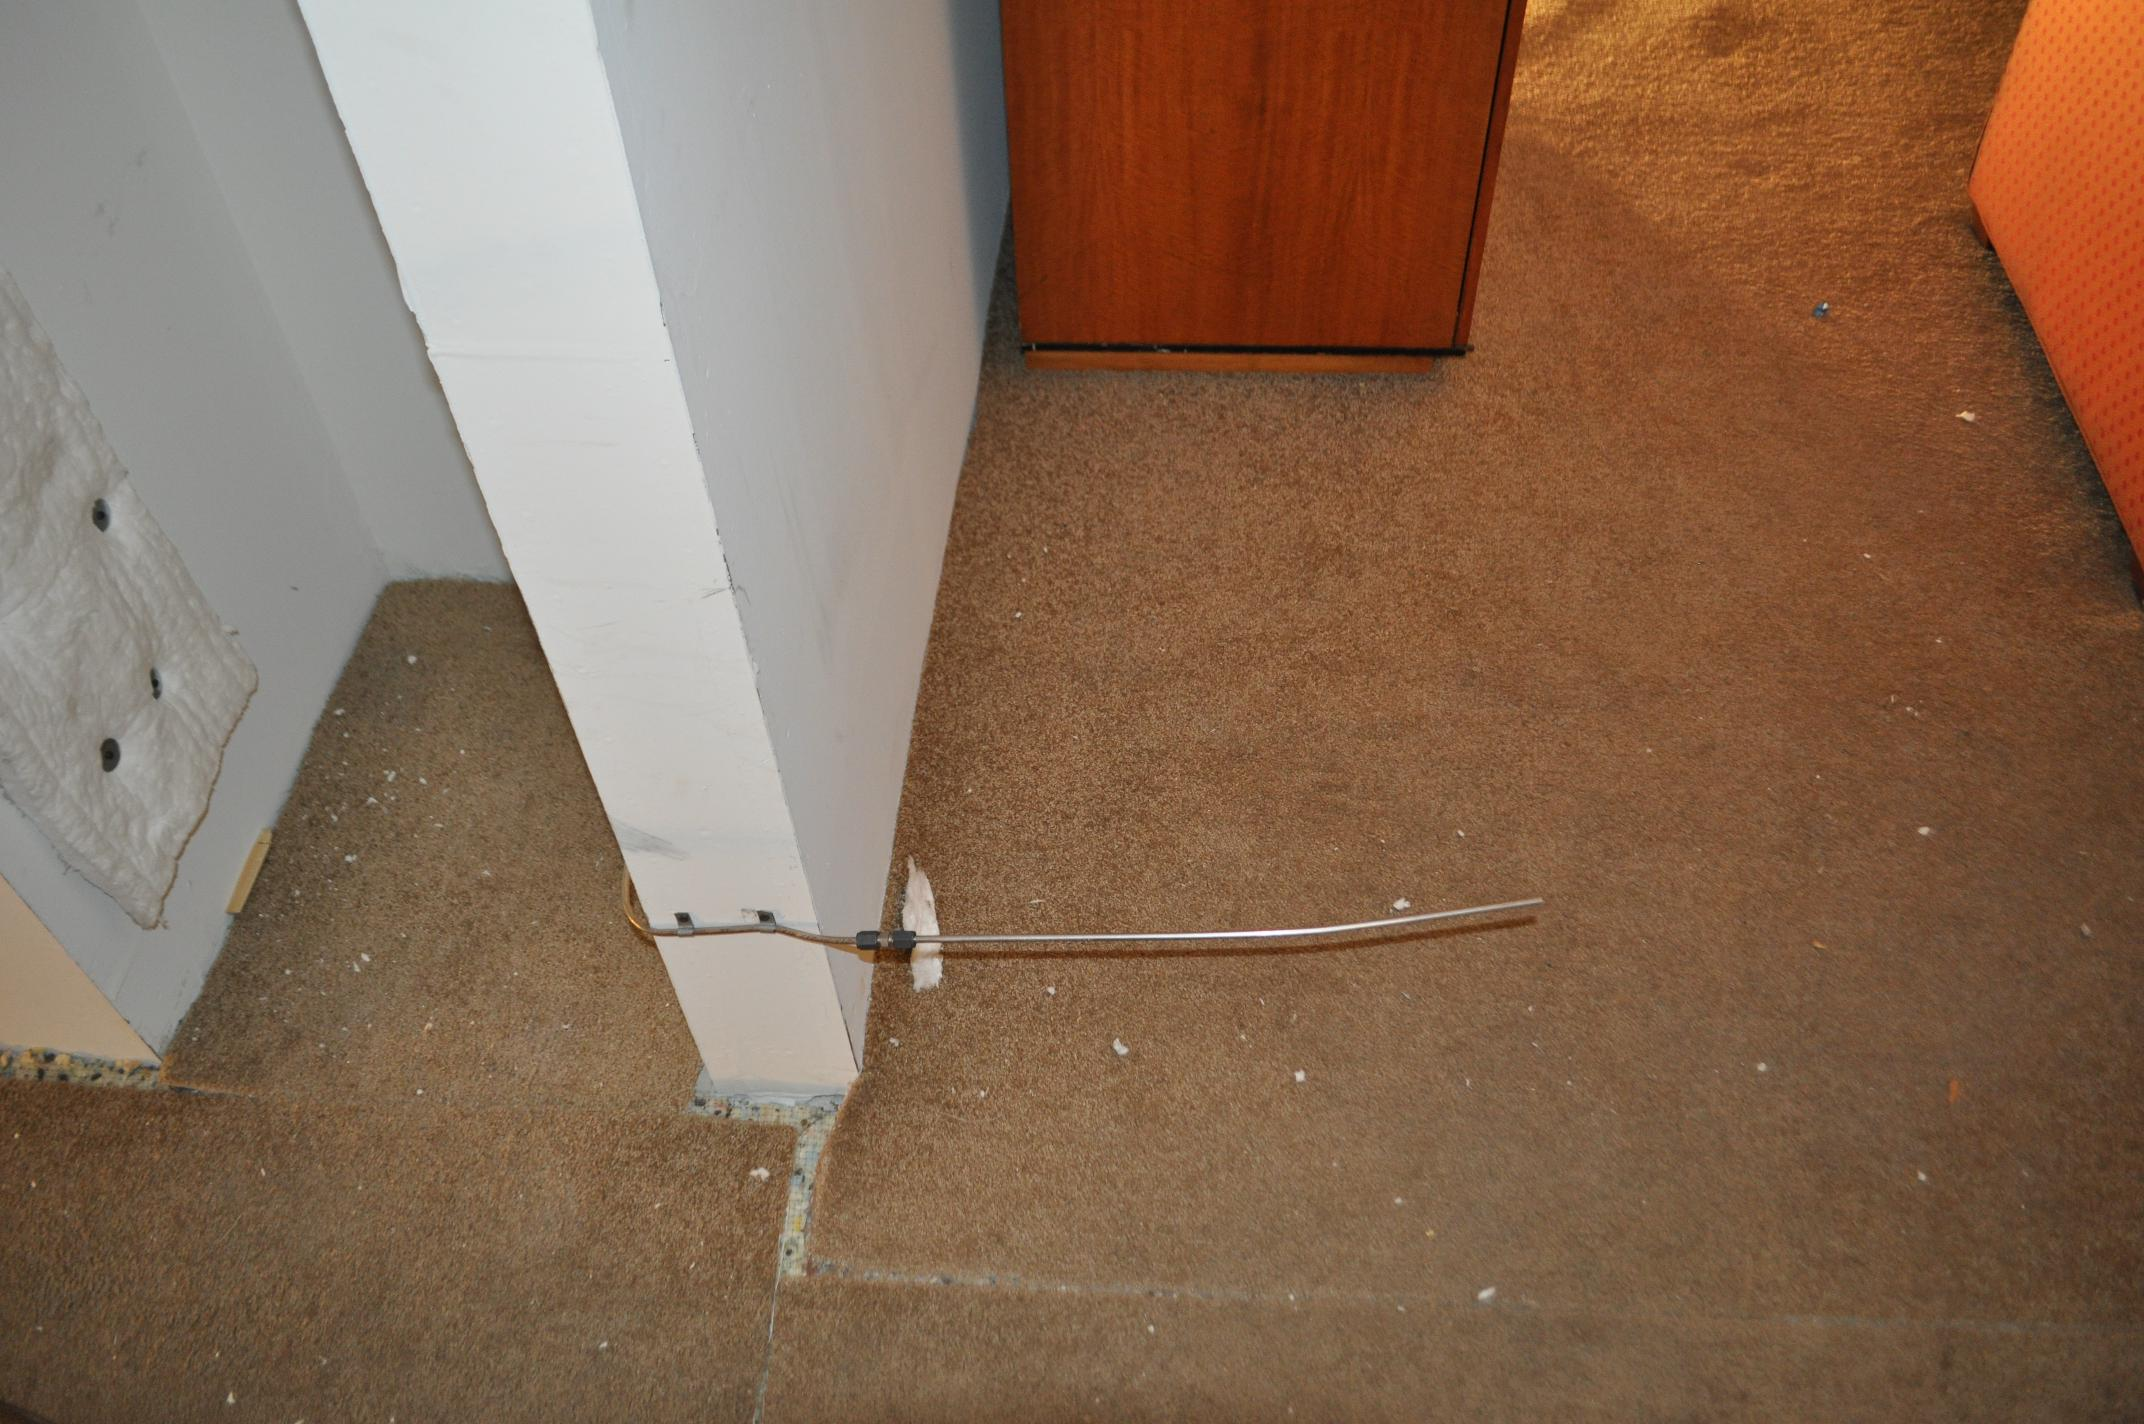
\includegraphics[width = 2in]{0_Images/Instrumentation/Gas_Analyzer/SamplePoint.jpg}
	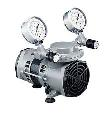
\includegraphics[width = 2in]{0_Images/Instrumentation/Gas_Analyzer/VaccumPump.jpg}
	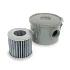
\includegraphics[width = 2in]{0_Images/Instrumentation/Gas_Analyzer/CourseFilter.jpg} \\
	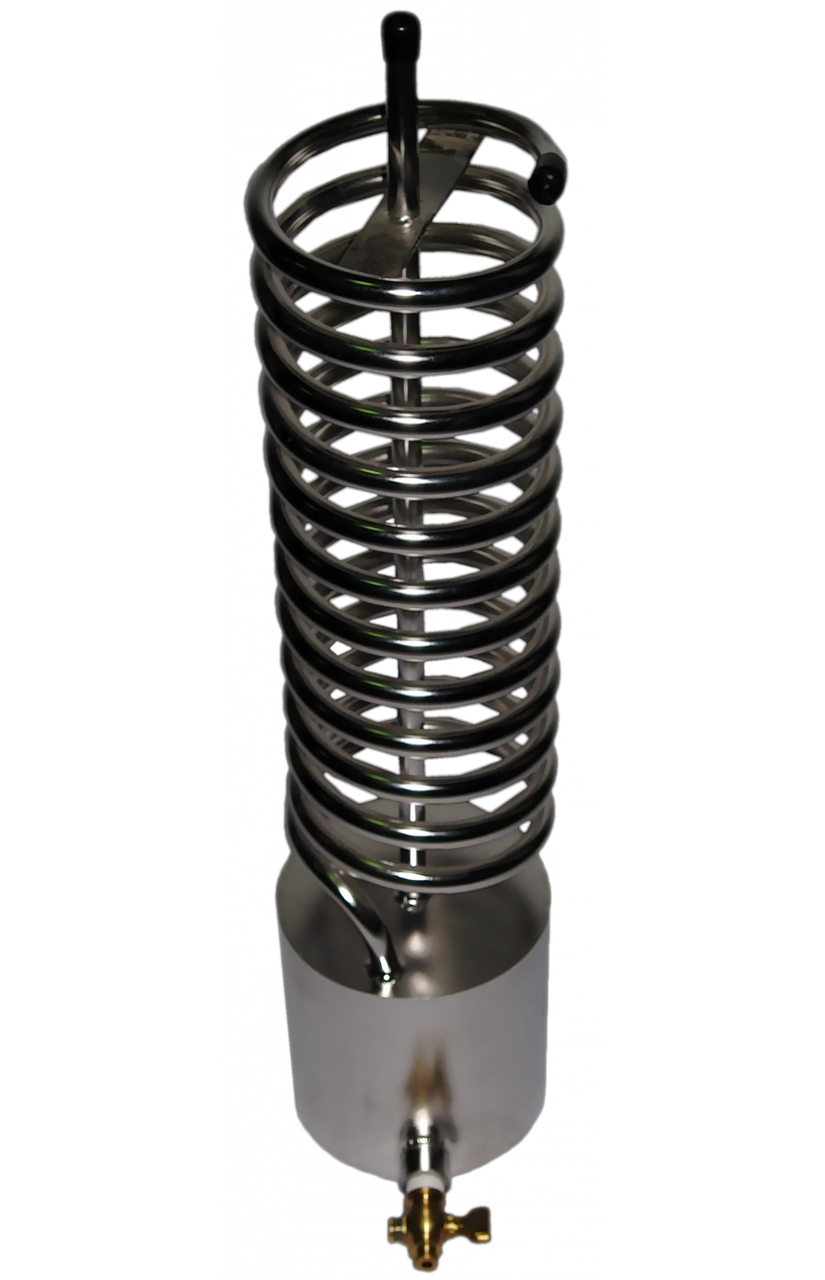
\includegraphics[height = 2in]{0_Images/Instrumentation/Gas_Analyzer/CoilCondenser.png} \hspace{0.1\textwidth}
	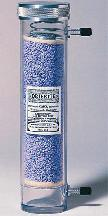
\includegraphics[height = 2in]{0_Images/Instrumentation/Gas_Analyzer/DriRightTube.jpg}	\hspace{0.1\textwidth}
	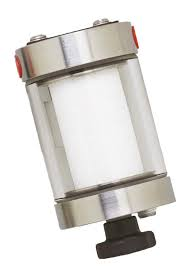
\includegraphics[height = 2in]{0_Images/Instrumentation/Gas_Analyzer/FineFilter.jpg} \\
	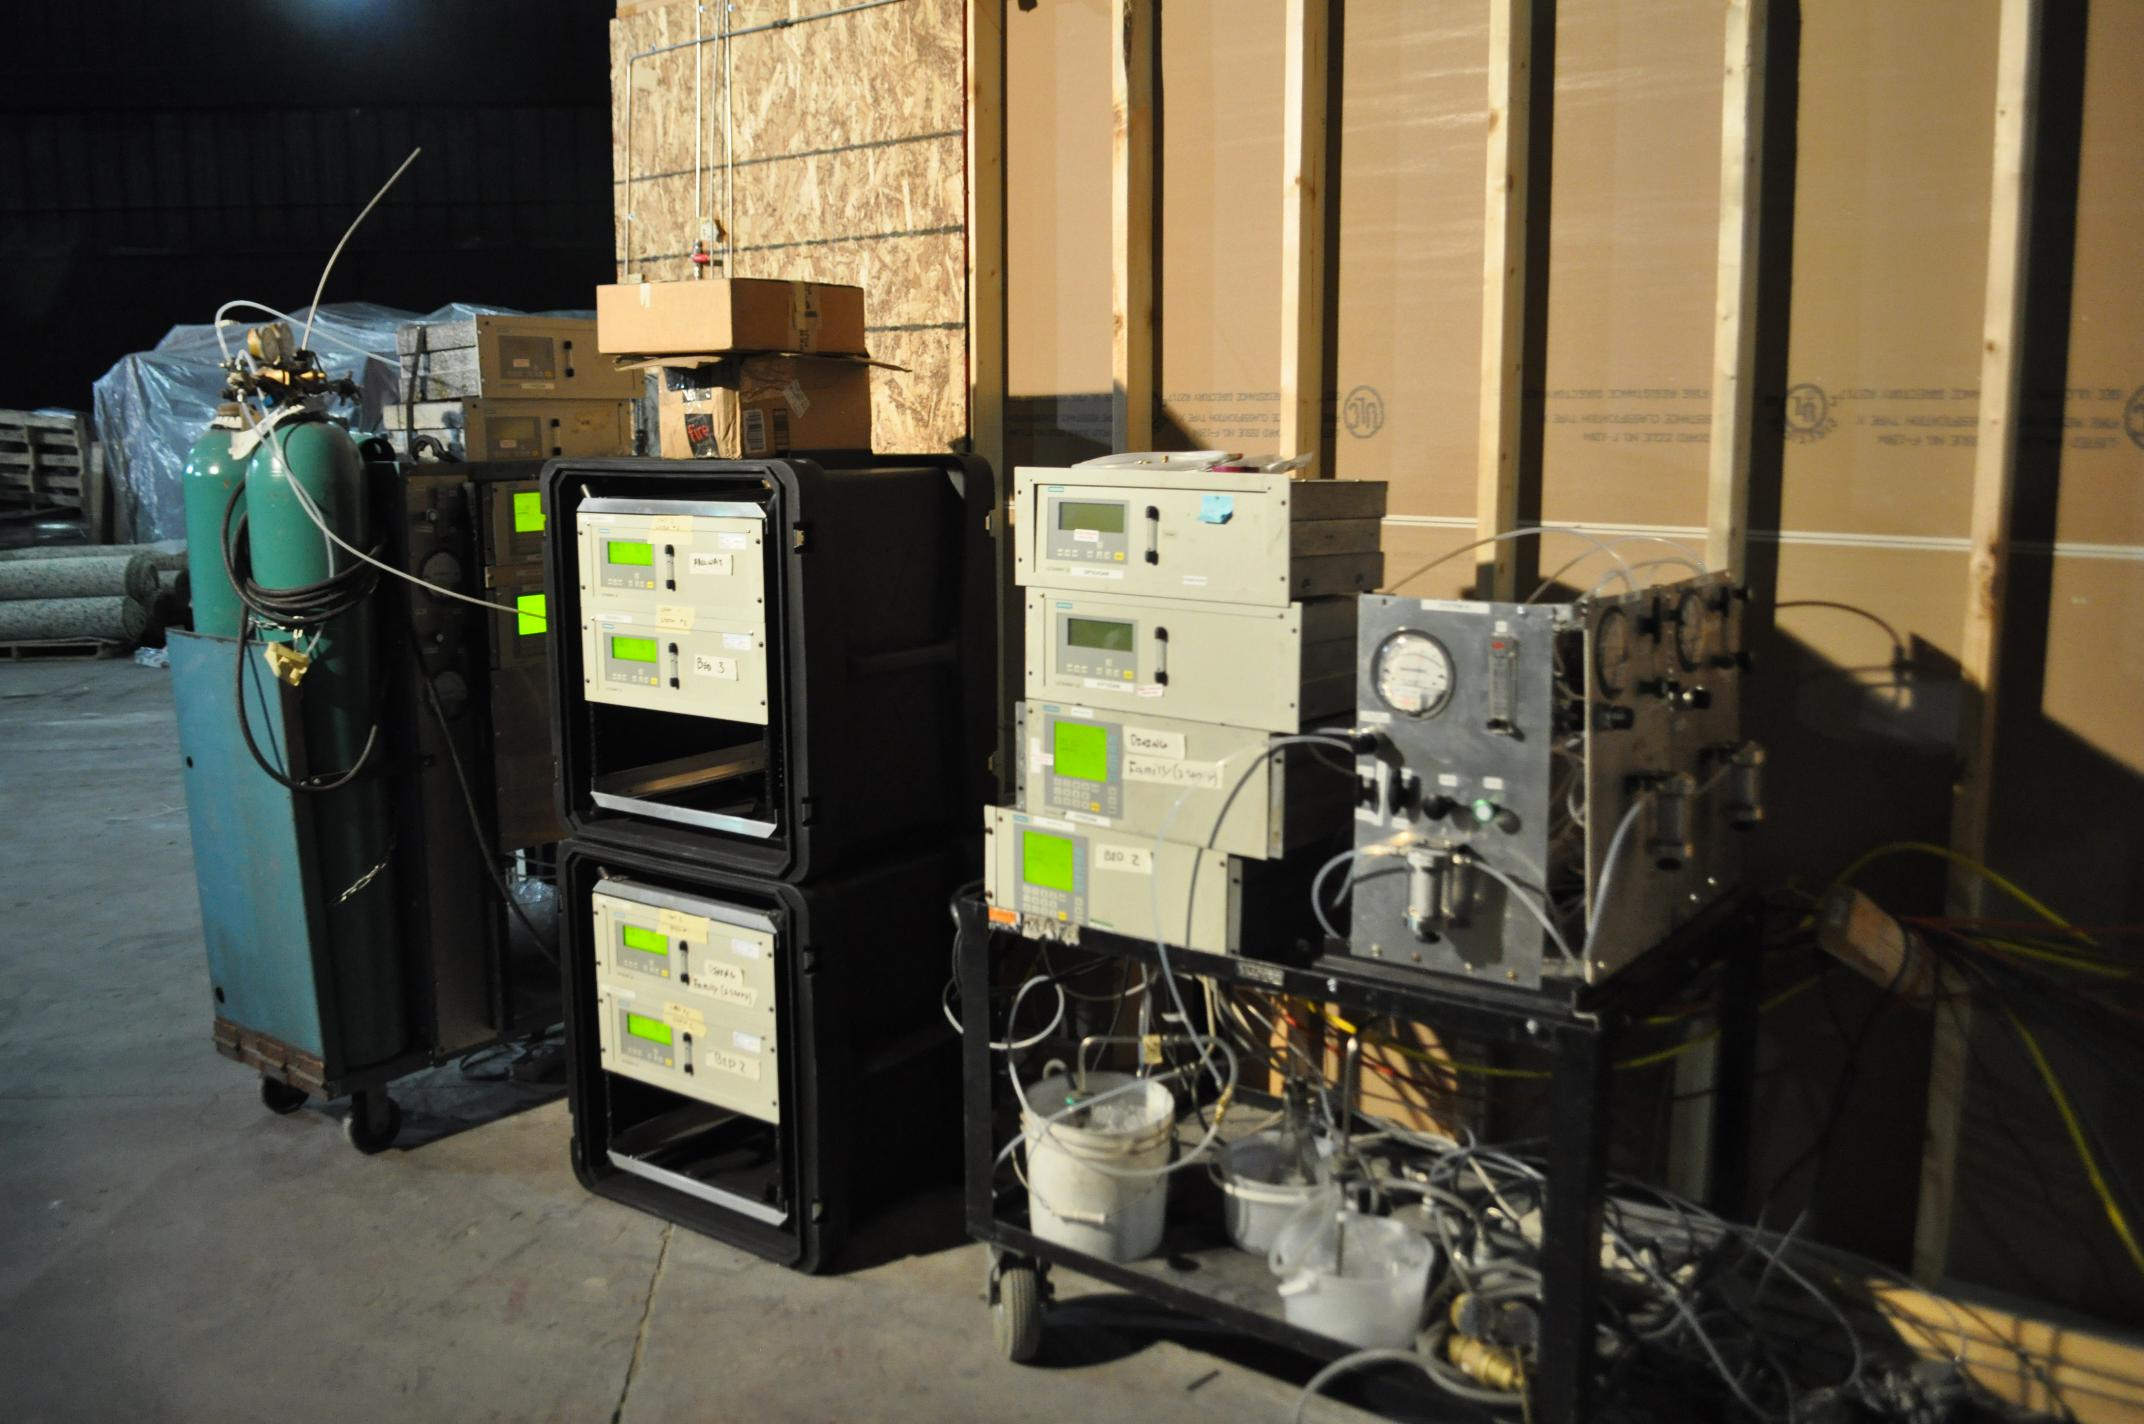
\includegraphics[height = 2in]{0_Images/Instrumentation/Gas_Analyzer/GasAnalyzers.jpg}
	\caption[Gas Analyzer Configuration]{Gas Analyzer Configuration, Gas Sample Point (Top Left), Vacuum Pump - Cole Palmer L-79200-30 (Top Center), Course Filter - Solberg 842 (Top Right), Condensing Tube (Middle Left), Drierite Tube (Middle Center), Fine Filter - Perma Pure FF-250-SG-2.5G (Middle Right), Gas Analyzer (Bottom)}
	\label{fig:GasAnalyzers}
\end{figure}

All data was logged through the use of a national instruments data acquisition system incorporating a SCXI-1001 chassis with 8 SCXI-1102C 32-Channel modules (Figure \ref{fig:DataSystem}). The system is configured for a total of 256 channels capable of reading values between 0-10~volts DC. Values are recorded once a second and translated to quantities of interest through the use of LabVIEW software specifically programmed for use with the system. Data was sampled at 1~hz across all channels.

\begin{figure}[H]
	\centering
	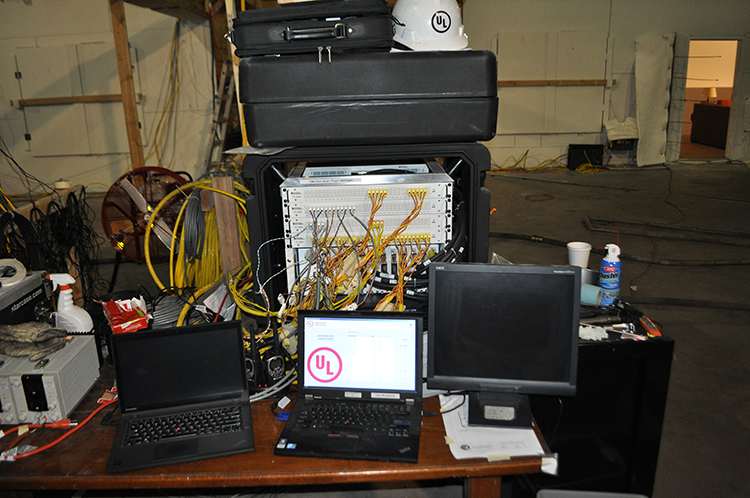
\includegraphics[width = 4in]{../0_Images/Instrumentation/DataSystem.jpg}
	\caption{Data Acquisition System}
	\label{fig:DataSystem}
\end{figure}

At the University of Illinois, Professor Tonghun Lee's research lab has advanced multiple laser based measurement techniques to quantify production of gases during internal combustion engine operation that have potential to be adapted to the sooty, dynamically changing live-fire environment. While there are a large number of techniques to measure moisture, most are not applicable to the situation of high temperature moisture measurements in a combustion environment.  Absorption spectrometry is capable of measuring moisture content in harsh, high temperature environments.  Water has several absorption bands in the near-infrared range, which allows the use of several classes of laser based systems to measure the moisture content.  With proper thermal and optical control of the laser source and sample train this technique is operable at temperature exceeding 1000 $^\circ$C (1832~$^\circ$F), can operate in and compensate for sooty and smoky environments, and has a very rapid response time on the order of seconds.  Such approaches have been utilized to perform in-situ analysis from controlled combustion and process exhaust systems.  The method used for these experiments was Tunable near-infrared diode laser to measure the water absorption peak near 1392 nm. Figure \ref{fig:Laser} shows the setup used in the experiments.

\begin{figure}[H]
	\centering
	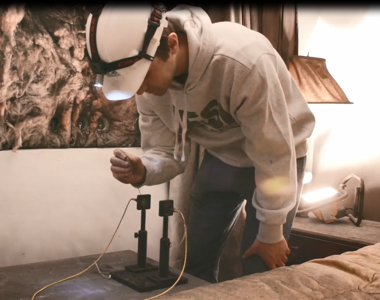
\includegraphics[height = 2.35in]{0_Images/Instrumentation/Laser1}
	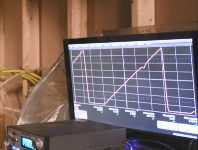
\includegraphics[height = 2.35in]{0_Images/Instrumentation/Laser2}
	\caption{Near-Infrared Diode Laser System}
	\label{fig:Laser}
\end{figure}

\clearpage

\section{Victim Package Instrumentation}

\subsection{Background}
Occupants trapped within a structure face the risk of thermal burn injuries, particularly with unprotected skin.  Suppression activities by the Fire Service can reduce this hazard by removing the heat source producing potentially dangerous conditions, however, the additional risks encountered by the conversion of water to steam must be studied.  The risk for moisture related skin burns is likewise present for firefighters applying water to burning materials from inside the structure.  While firefighting PPE provides a significant measure of protection, burn injuries are still a significant hazard during interior firefighting operations.

The dangers of thermal injury from exposure to heat and products of combustion and time-temperature characteristics required for skin burns has been researched for several years.  Typical studies involve exposing skin to a controlled thermal exposure and the time to an outcome, such as dermal or epidermal temperature changes (typically time to reach 44.8~$^\circ$C (113~$^\circ$F)) or visual indications of damage. The synergistic effect of elevated temperature and moisture content on increasing risk for skin burns is conceptually understood to be due to the large latent heat and partial pressure of water at temperatures above 60~$^\circ$C (160~$^\circ$F).  However, the effect of suppression tactics and the rapidly changing transient nature of exposure during this time frame (ambient temperatures reducing while the moisture content is increasing) on risk for skin burns has not been measured in response to realistic fire suppression experiments. 

An important objectives of the study is to better understand the influence of water application to a room and contents fire on trapped occupant exposure - particularly with respect to changing the risk for steam burns. Traditional measurement techniques utilized to estimate thermal risk (thermocouple to measure air temperature and heat flux gages to estimate thermal energy available to increase temperature of surfaces such as skin) are commonly utilized to estimate exposures through techniques such as the ISO standard fractional effective does (FED) tenability method.  However, there are some important limitations to this these techniques and assumptions must be made.  The impact of rapidly changing moisture conditions and the interaction of skin with radiation can have significant impact on the results.  In order to more accurately measure the impact of typical live-fire environment on human skin, an ex vivo porcine skin model was developed as a means of estimating the human skin exposure. Porcine skin has often been used as a surrogate for human skin in scientific study \cite{Pig_Experimental_model,Of_pigs_and_men,Sensitivity_Cross-reacting}, due to the number of similarities between pig skin and human.  Utilizing this approach along with traditional fire estimation methods will hopefully provide new understanding of risks for trapped occupants and possibly provide a pathway for calibration of the existing tools to better estimate this risk.   

Human skin is the largest organ in the human body, providing important protective and heat transfer biological function.  The skin is comprised of several important components that are typically grouped in three distinct layers.  The epidermis is the outer layer of skin, comprised of dead cells and acts as the protective barrier to harmful environmental conditions such as moisture, ultraviolet radiation, and extreme heat \cite{Hummel_Barker_Lyons}. Only part of the epidermis is effected in first degree burns and the dead cells flake off following the burn \cite{Purser_Toxicity_Heat,Hummel_Barker_Lyons}. The human epidermis fluctuates based on body site and has been measured using ultrasonography to vary from less than 40~$\mu$m (0.002~in) on the cheek and portions of the truck to over 350~$\mu$m (0.014~in) on the fingertip \cite{Epidermis_Thickness}. Typical ranges in thickness from 50~$\mu$m (0.002~in) to 120~$\mu$m (0.005~in) are reported \cite{Pigs_Wound_Healing}. 

\begin{figure}[H]
\centering
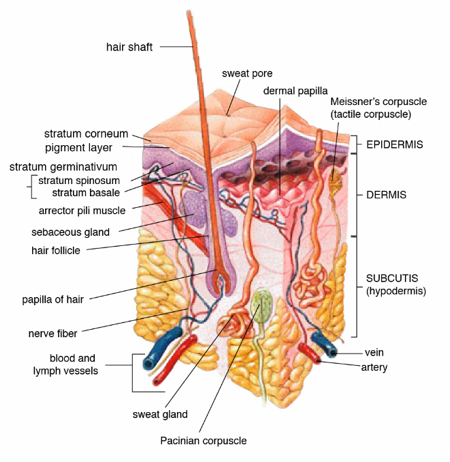
\includegraphics[width=0.5\textwidth]{../0_Images/Instrumentation/Burn_Measurements/human_skin}
\caption{Cross Section of Human Skin}
\label{fig:inst_human_skin},
\end{figure}

The dermis is the second layer of skin which contains important living tissues such as blood vessels and nerve endings \cite{Hummel_Barker_Lyons}. Second degree burn occurs when the damage reaches the dermis layer, completely destroying the epidermis \cite{Hummel_Barker_Lyons}. Blisters can form in the area between the basal layer of the epidermis and dermis \cite{Purser_Toxicity_Heat}. Like the epidermis, the human dermis fluctuates in thickness from less than 1000~$\mu$m (0.04~in) to 4000~$\mu$m (0.16~in) based on the area of the body \cite{Skin_Pulse,Visualization_Thickness}.

When at least 75\% of the dermis has been destroyed and the burn extends to the subcutaneous layer, full necrosis has occurred resulting in a third degree burn \cite{Purser_Toxicity_Heat}. The subcutaneous layer is the deepest layer of skin and is comprised of fat and connective tissue \cite{Hummel_Barker_Lyons}.

Domestic pigs are have been used for decades as surrogates for humans in experiments. The skin of a domestic pig is one feature that is similar to humans in many aspects such as thickness, structure, and composition \cite{Time_Temperature_Cutaneous_Burns}. Pig skin and human skin both have similar proteins, a sparse hair coat, a thick epidermis, a dermis with a papillary body, a deep layer of subcutaneous fat, and a large content of elastic tissue \cite{Of_pigs_and_men}. Normal pig skin varies by body site just as human skin does. The pig epidermis is described as ranging in thickness from 70~$\mu$m (0.003~in) to 140~$\mu$m (0.006~in) compared to the human epidermis range \cite{Pig_Experimental_model}. Due to the range of skin thickness throughout the body, a dermal-epidermal ratio ranging from 10:1 to 13:1 proves to be a better measure of thickness and is again, comparable in both pig and human skin \cite{Pigs_Wound_Healing}.  It has been suggested that the structure of the pig's skin is so similar to that of a human skin, that it may be a more{} superior model than that of nonhuman primate skin \cite{Sensitivity_Cross-reacting}. However, there are important differences such as a lower water loss from pig skin at elevated temperatures and lack of blister formation that must be considered when using this model.

Moritz and Henriques conducted a series of experiments with both humans and pigs, such as creating contact burns at different temperatures and durations of time \cite{Time_Temperature_Cutaneous_Burns}. Their study demonstrated irreversible damage will occur to the epidermis when the surface of skin reaches 44~$^\circ$C (111~$^\circ$F), although it can take long periods of exposure. Below this temperature, the rate of recovery exceeds the rate of damage due to burning \cite{Thermal_Electronic}. The time required to create irreversible damage is reduced by about half with every degree increase between 44~$^\circ$C (111~$^\circ$F) and 55~$^\circ$C (131~$^\circ$F) \cite{Thermal_Electronic}\hl{[?]}. Third degree burns can occur within one second of exposure once the skin reaches temperatures ranging from 57~$^\circ$C (135~$^\circ$F) to 63~$^\circ$C (145~$^\circ$F) \cite{Thermal_Electronic}\hl{[?]}. Stoll and Green continued the work of Moritz and Henriques and discovered that the destruction of the skin does not only begin when the surface rises above 44~$^\circ$C (111~$^\circ$F), but continues as long as the temperature of the layer remains at 44~$^\circ$C (111~$^\circ$F) or higher \cite{Pain_Thermal_Radiation}. This means that the cooling phase also needs to be included in pred{}i{}cting methods \cite{Standard_Manikin}. Stoll et al. found that destruction rate can be modeled by the following first order chemical reaction rate equation.  With the use of this approach, burn injury becomes a function of the time and temperature when the skin exceeds 44~$^\circ$C (111~$^\circ$F). 

\subsection{Victim Instrumentation Packages}
A new method for estimating skin burn risk based on ex vivo samples of porcine (pig) skin has been developed. Figure \ref{fig:inst_SBA} shows the design and instrumentation of the victim package experimental setup. The victim package provides a transportable system for exposing skin samples to live-fire conditions in relatively repeatable conditions.  Up to 6 excised porcine skin samples (surrogate for human epidermal and dermal layers) are introduced on top of 10~mm (0.4~in) thick neoprene rubber slab (surrogate for subcutaneous fat), which sit on top of a basin holding water at 36.7 to 37.8 $^circ$C (98-100$^\circ$F) (simulate the core of the body).  Each exposed skin sample had an exposed surface area of 10~cm x 10~cm (4~in x 4~in) to improve the applicability of a one-dimensional heat transfer scenario (through the skin as opposed to across the skin).  Neoprene was used for subcutaneous fat as it has similar thermal and mechanical properties as well as providing a uniform thickness. The thickness of the neoprene was used to simulate the thickest layers of subcutaneous fat. Strips of insulation were used to cover the exposed aluminum on the top of the plate and insulation was wrapped around the basin to help maintain the water bath temperature at human core body temperature. 


\begin{figure}[H]
\centering
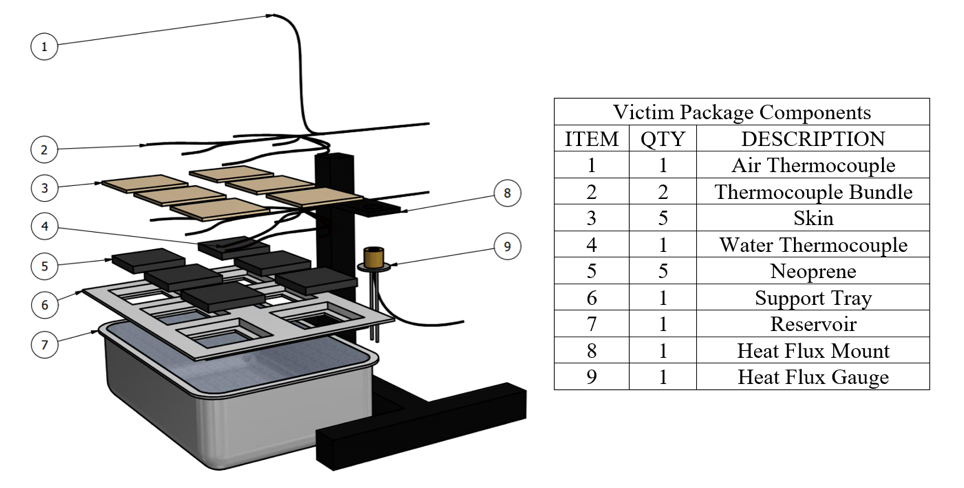
\includegraphics[width=0.5\textwidth]{../0_Images/Instrumentation/Burn_Measurements/Skin_Burn_Assessment_Package}
\caption{Exploded CAD view of Victim instrumentation Package}
\label{fig:inst_SBA}
\end{figure}

Type K thermocouples were attached to the surface of the neoprene layer to measure sub-dermal temperature using cyanoacrylate glue.  Furthermore, an identical thermocouple was placed in the center on the surface of the skin sample after it was deployed.  Additionally, thermocouples were also used to measure the temperature of the air surrounding the victim packages and to measure the temperature of the water bath during the test to ensure core body temperature was closely maintained.  Vertically oriented heat flux gages were deployed at each location to measure the thermal energy reaching the skin samples.  As part of the instrumentation package, local measurements of gas concentration (O$_2$, CO$_2$, CO) were also measured at each of these locations.

\begin{figure}[H]
\centering
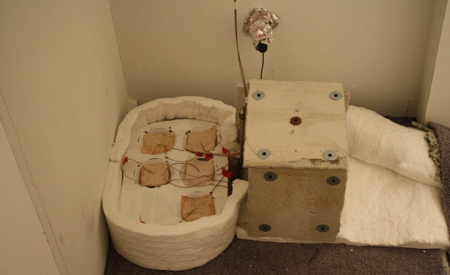
\includegraphics[width=0.5\textwidth]{../0_Images/Instrumentation/Burn_Measurements/SBA_Deployed}
\caption{Victim Instrumentation Package Installed}
\label{fig:inst_SBA_deployed}
\end{figure}

\subsubsection{Sample Preparation and Victim Instrumentation Package Deployment}
Porcine skin samples were collected from research animals at the University of Illinois after they were euthanized for purposes other than this project. The epidermal/dermal layer was removed immediately from the carcass.  After transportation to the lab, subcutaneous fat was removed and the hair was shaved from the top layer of the skin using a razor. The sample was then placed in a plastic bag and stored in a freezer until the live-fire scenarios were to be conducted. Before being deployed into an experiment, the skin was thawed in the plastic bags using a water bath held at 37~$^\circ$C (98.6~$^\circ$F) one hour before the experiment began. After the sample was fully thawed, the skin was removed from the bag and its thickness was measured. The average porcine skin thickness in these victim packages was 3.66$pm$ 0.72~mm or approximately 3660$\mu$m (0.14~in).  

The samples were then deployed to their locations and attached to the neoprene blocks using cyanoacrylate glue and surface thermocouples were similarly deployed. Damp towels were placed over the specimens to ensure they did not dry out prior to testing and heater and pumps were used to control the water bath temperature. Five minutes before the experiment began, the damp towels were removed and the structure was properly closed off. The temperature of the skin prior to the start of the experiment was typically between 27.8-33.2~$^\circ$C (82-92$^\circ$F) which is representative of human skin temperatures, depending on the area of the body.

For these scenarios, victim packages were deployed to 5 different locations throughout the structure (Figure \ref{fig:instruments}.  Locations 1, 4, and 5 were placed on the floor, while 2 and 3 were on top of a bed. The top of the bed was 0.7~m (2.2~ft) above the floor.  The bedroom door at the entrance to location 2 was closed throughout each scenario.  


\begin{figure}[H]
\centering
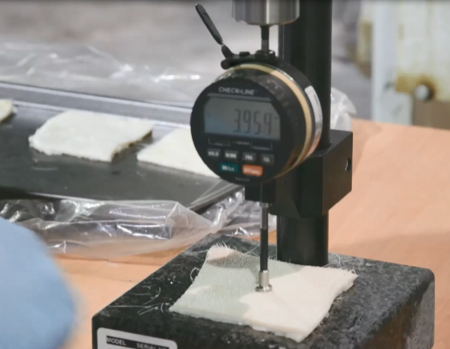
\includegraphics[width=0.495\textwidth]{../0_Images/Instrumentation/Burn_Measurements/SBA_Measurment}
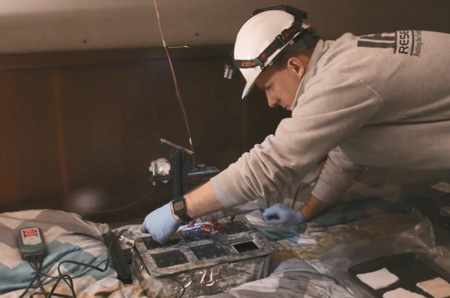
\includegraphics[width=0.495\textwidth]{../0_Images/Instrumentation/Burn_Measurements/SBA_Sub_TC_Attach}
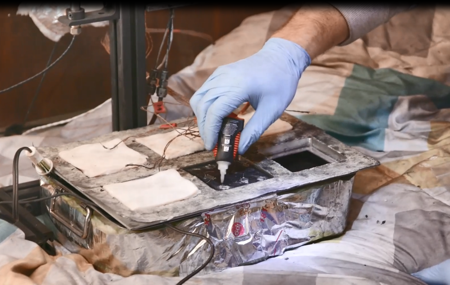
\includegraphics[width=0.495\textwidth]{../0_Images/Instrumentation/Burn_Measurements/SBA_gluing}
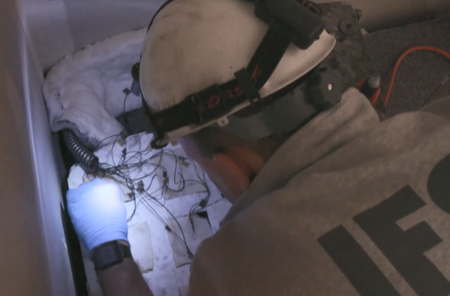
\includegraphics[width=0.495\textwidth]{../0_Images/Instrumentation/Burn_Measurements/SBA_Sur_TC_Attach}
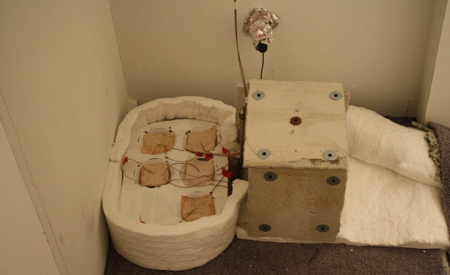
\includegraphics[width=0.495\textwidth]{../0_Images/Instrumentation/Burn_Measurements/SBA_Deployed}
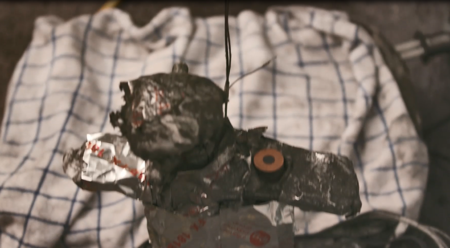
\includegraphics[width=0.495\textwidth]{../0_Images/Instrumentation/Burn_Measurements/SBA_Damp_Towel}
\caption{Sample prep including thickness measurement, sub-dermal thermocouple attachment (note heating element and circulation pump on left to maintain core ``temperature''), gluing skin samples to subcutaneous fat surrogate, surface TC attachment, final victim package (location \#1) and damp towel placement that is removed immediately prior to ignition.}
\label{fig:inst_SBA_Prep}
\end{figure}


\section{Measurement Locations}

In order to collect the data needed for this analysis, sensors were installed and measurements were recorded throughout each structure. Figure \ref{fig:instruments} shows the location and numbering scheme for the instruments utilized. 

\begin{figure}[H]
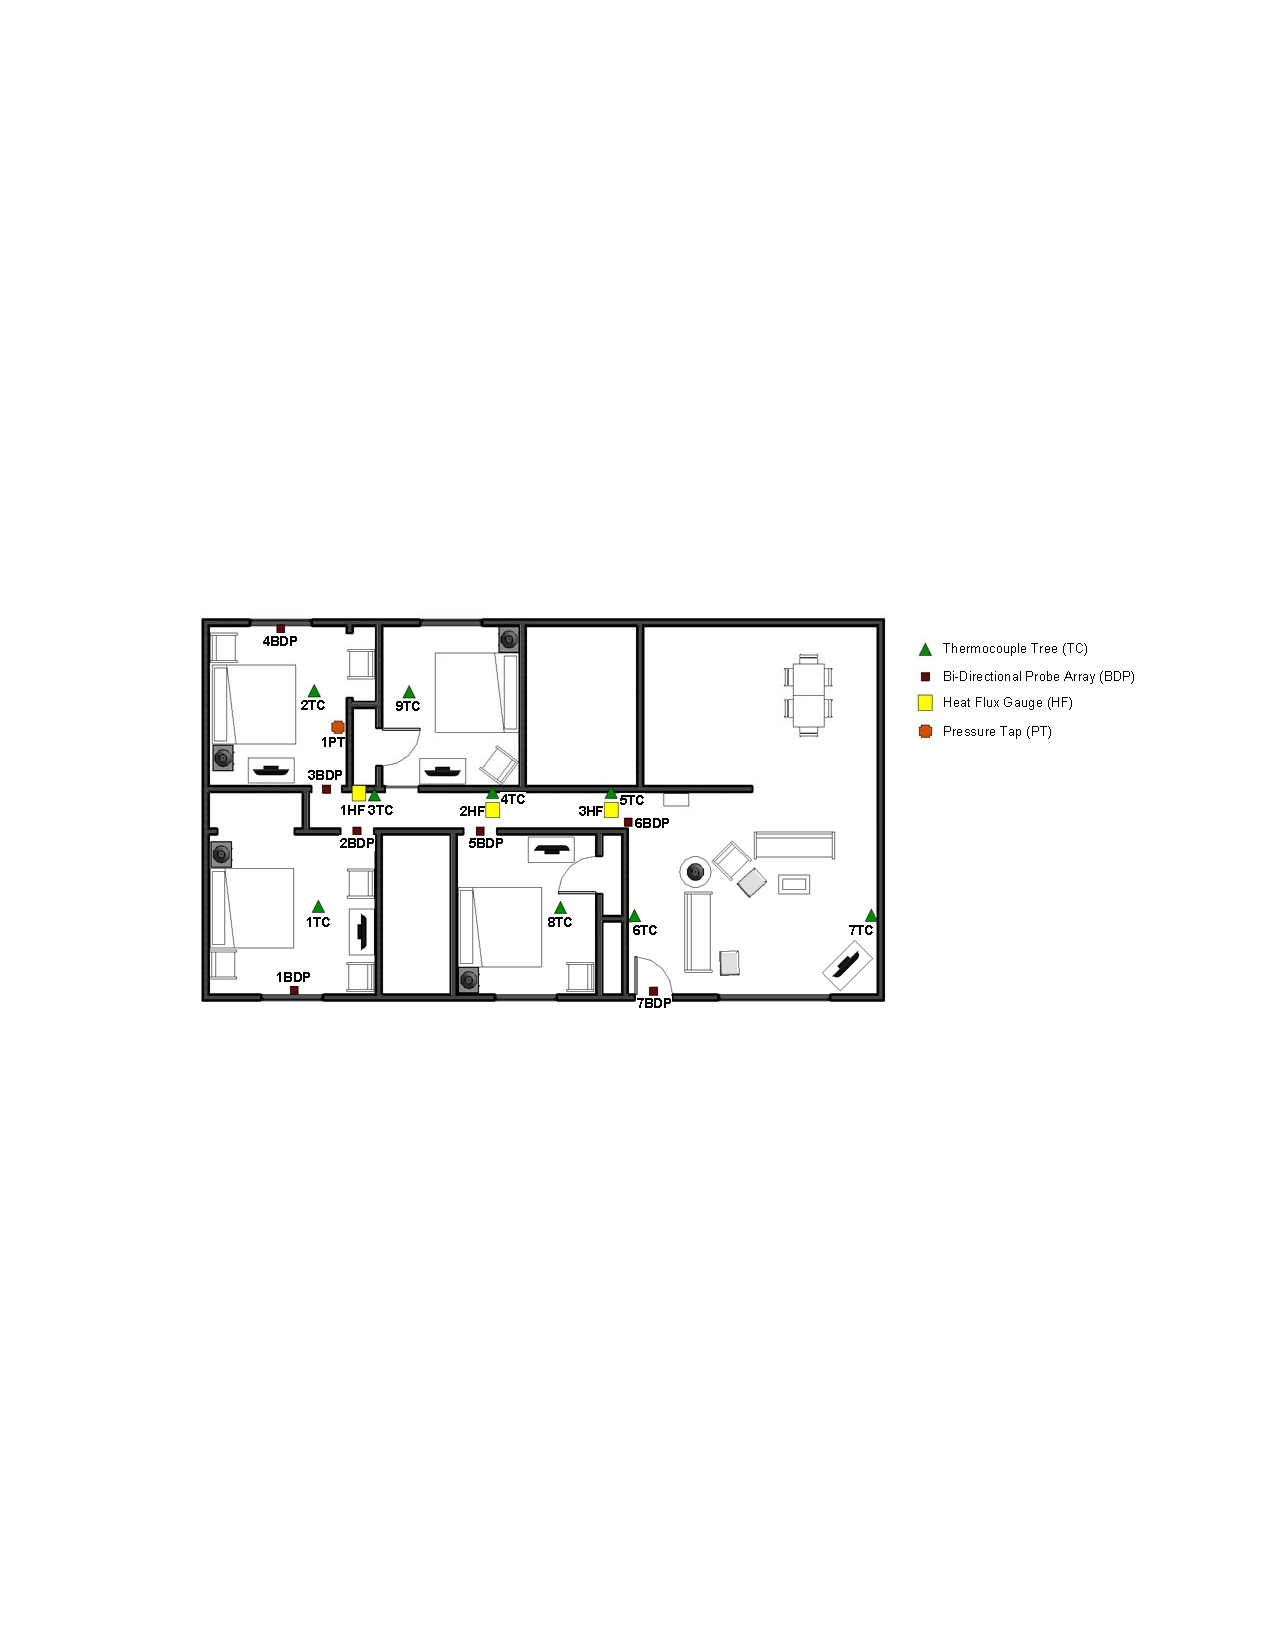
\includegraphics[width=.75\textheight]{0_Images/Ranch_Pictures/Instrument_Plan}
\caption{Instrumentation Plan}
\label{fig:instruments}
\end{figure}

Cameras were located throughout the structure to provide visual data. Figure \ref{fig:cameras} shows the location and type of cameras utilized in the experiments.

\begin{figure}[H]
	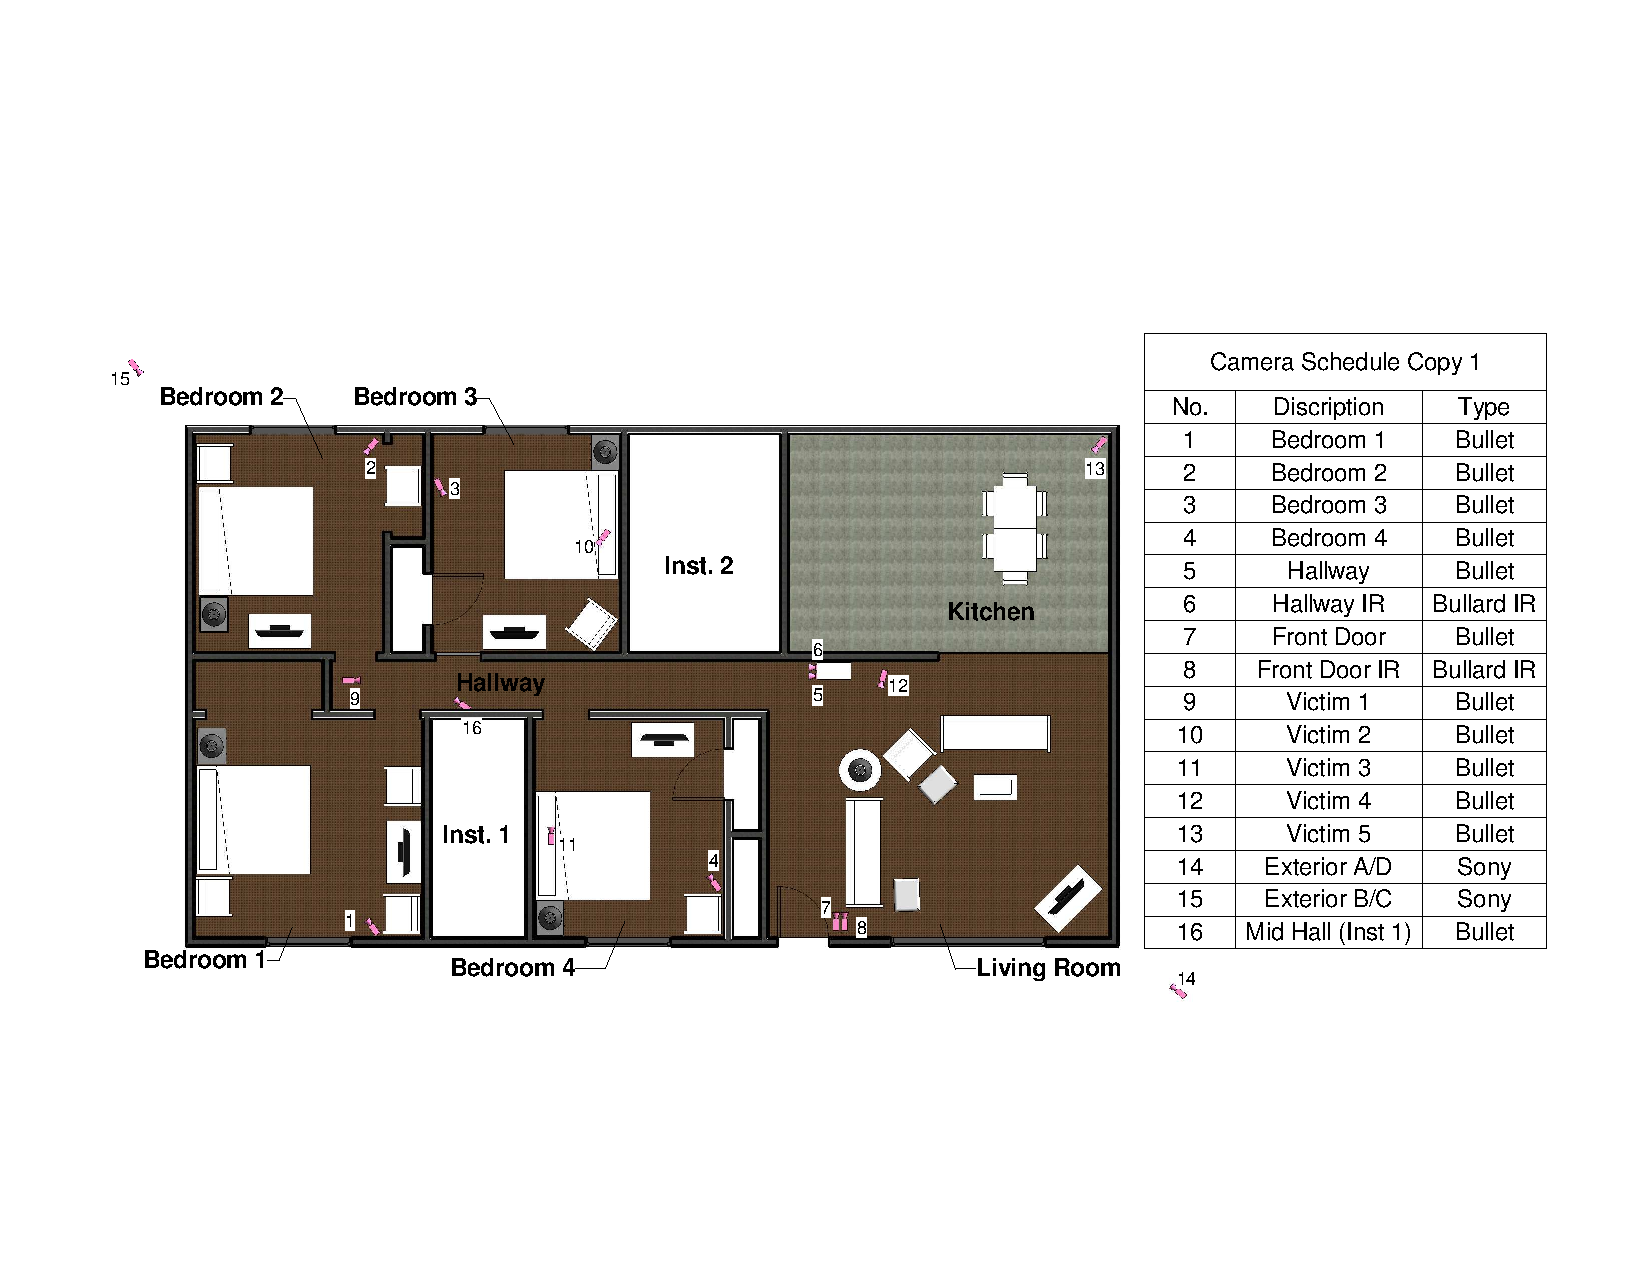
\includegraphics[width=.75\textheight]{0_Images/Ranch_Pictures/Camera_Plan}
	\caption{Camera Plan}
	\label{fig:cameras}
\end{figure}
\clearpage 

\section{Equipment Utilized}

In order to limit the number of variables, two nozzles were selected for use during the full scale experiments. Part I \cite{Weinchenk_watermapping} and Part II \cite{Weinchenk_airentrainment} of this project highlighted that no statistically significant difference exists between manufacturers in terms of air entrainment and rated flow for a given nozzle type and stream configuration. To most closely match the flow and pressure of a single smooth bore nozzle with a single combination nozzle the nozzles listed Table~\ref{table:nozzle_selection} were selected. 

\begin{table}[H]
\caption{Nozzle Selection}
\centering
\begin{tabular}{|l|c|c|c|}
\hline
Nozzle 		& Tip (in) 	& Nozzle Pressure (psi)	& Approximate Flow Rate (gpm) \\ \hline \hline
Smooth Bore & 	7/8 	& 	50 					& 160 \\ \hline
Combination & 	N/A 	& 	75 					& 150 \\ \hline
\end{tabular}
\label{table:nozzle_selection}
\end{table}

The nozzles were connected to 200~ft of 1 3/4~in hoseline. Pressure was set utilizing a in-line water filled pressure gauge just behind the nozzle. Real time flow was measured with a 3~in electromagnetic flow meter, connected prior to the 200~ft of hoseline. %as shown in Figure \hl{NEED A PICTURE OF FLOW METER}. 


\clearpage

\section{Suppression Tactics Utilized}

The method of approaching a residential fire varies greatly depending on shift, department, state and region. It was not possible to test all the variations so the project technical panel was polled and the methods used by their representative department/shifts were analyzed and grouped into three major methods. The three methods utilized were titled `Shutdown \& Move Advancement', `Flow \& Move Advancement' and `Transitional Attack'. Where experiments permitted slight variations, those variations were incorporated to understand their impact on the overall suppression tactic.

% \begin{table}[H]
% 	\centering
% 	\caption{Tactics Utilized}
% 	\begin{tabular}{|c|c|c|} 
% 		\hline
% 		Shutdown \& Move & Flow \& Move & Transitional Attack \\ \hline \hline
% 		Front Door Open & Front Door Open \\ \hline
% 		Read of Conditions & Read of Conditions \\ \hline
% 		Attack Team Entry & Attack Team Entry\\ \hline
% 		Burst Suppression - "Check for Return" & Burst Suppression - "Check for Return" \\ \hline
% 		% Position at start of hallway and begin flowing & Position at start of hallway and flow from fixed position (5-10 sec) \\ \hline
% 		% Flow down hallway from close to far in a wall-ceiling-wall pattern while advancing until final room suppression & Flow from middle of hallway (5-10 sec) \\ \hline
% 		%  & Final Room Suppression at End of Hall
% 	\end{tabular}
% 	\label{Table:Tactics}
% \end{table}

\subsection{Flow \& Move Advancement}
The `Flow \& Move Advancement' incorporated moving the hoseline (advancing) while flowing water. This was not employed until the crew was in position at the start of the hallway, moving towards the fire compartment at the end of the hall. The tactic was conducted utilizing the following steps in order:

\begin{itemize}
	\item{Front door open.}
	\item{Read neutral plane and conditions at entry door (10~seconds).}
	\item{Suppression crew enters to a position approximately 3~ft inside the door.}
	\item{Burst Suppression - ``Check for Return'', crew flows a short burst of water at the ceiling.}
	\item{Suppression crew advances to the start of the hallway.}
	\item{Flow down hallway from close to far in a `wall-ceiling-wall' pattern while advancing until arriving at the fire compartment.}
	\item{Without shutting down the line, suppression crew applied water to the fire compartment.}
	\item{Once fire was `under control' the crew paused 1~minute to evaluate conditions.}
	\item{Suppression crew entered the fire compartment for final suppression.}
	\item{All windows were opened for ventilation}
\end{itemize}

This tactic involved variation in the nozzle type (smooth bore, combination straight stream, combination fog) and the use of burst suppression between experiments to evaluate the impact.

\clearpage

\subsection{Shutdown \& Move Advancement}
The `Shutdown \& Move Advancement' incorporated the same tactics as the `Flow \& Move Advancement' with the exception that the suppression crew was not moving the hoseline (advancing) while flowing water. The tactic was conducted utilizing the following steps in order:

\begin{itemize}
	\item{Front door open.}
	\item{Read neutral plane and conditions at entry door (10~seconds).}
	\item{Suppression crew enters to a position approximately 3~ft inside the door.}
	\item{Burst Suppression - ``Check for Return'', crew flows a short burst of water at the ceiling.}
	\item{Suppression crew advances to the start of the hallway.}
	\item{Flow from fixed position (5-10~seconds) from close to far in a `wall-ceiling-wall' pattern.}
	\item{Advance to a position halfway down the hall.}
	\item{Flow from fixed position (5-10~seconds) from close to far in a `wall-ceiling-wall' pattern.}
	\item{Advance to the fire compartment and apply water into the compartment.}
	\item{Once fire was `under control', visible flames or audible signs of combustion were absent, pause 1~minute to evaluate effectiveness of tactic.}
	\item{Suppression crew entered the fire compartment for final suppression.}
	\item{All windows were opened for ventilation}
\end{itemize}

This tactic involved variation in the nozzle type (smooth bore, combination straight stream, combination fog) and the use of burst suppression between experiments to evaluate the impact. 

\clearpage

\subsection{Transitional Attack}
The transitional attack involved an initial exterior water application followed by interior suppression. The tactic was conducted utilizing the following steps in order:

\begin{itemize}
	\item{Exterior water application into the fire compartment.}
	\item{Approach compartment and wet surfaces (Not during all experiments)}
	\item{Reposition hoseline to front door}
	\item{Front door open.}
	\item{Suppression crew enters, flows water to cool as they approach, if necessary.}
	\item{Apply water to the fire compartment, if necessary}
	\item{Once fire was `under control' pause 1~minute to evaluate effectiveness of tactic.}
	\item{Suppression crew entered the fire compartment for final suppression.}
	\item{All windows were opened for ventilation}
\end{itemize}

This tactic involved variation in the nozzle type (smooth bore, combination straight stream, combination fog), if a secondary exterior application was conducted (second room of fire), flow on the advancement down the hallway, front door open prior to or after initial application of water, and need for application of water into the fire compartment from the interior. 

\chapter{Full-Scale Residential Fire Experiments}

In order to examine different fire attack techniques, twenty-five experiments were conducted in the full-scale residential structure described in Chapter~\ref{chap:exp_config}. Experiments~1--17 were focused on studying interior fire attack methods, and the remaining eight experiments were focused on studying transitional fire attack methods. Three different ventilation configurations were used throughout all 25 experiments: `No Vent', `Single Vent', and `Two Vent'. These configurations along with the details of each individual experiment are described in the following sections and Table ~\ref{table:summary_of_experiments}.  

Fire intervention times were based on conditions within the fire compartment(s) to ensure repeatable conditions and comparability of experiments. For experiments where no ventilation was provided, the point at which the fire became ventilation limited and temperatures began to decrease was the point where intervention began. For experiments where the window was open prior to ignition, the point at which the fire reached a steady, ventilation limited state was the time intervention began.

\clearpage

\begin{table}[!ht]
\caption{Summary of Experiments}
\centering
\scalebox{0.70}{
\begin{tabular}{|c|c|c|c|c|l|}
\hline
\multirow{2}{*}{Experiment} 	& Fire Attack 	& \multirow{2}{*}{Nozzle}		& \multirow{2}{*}{Advancement} 		& \multirow{2}{*}{Pattern}		& \multicolumn{1}{c|}{\multirow{2}{*}{Ventilation Parameters}} \\ 
								& 	Method	   	& 								& 									& 								& 										\\ 
\hline \hline
\multirow{2}{*}{1}	& \multirow{2}{*}{Interior} & \multicolumn{3}{c|}{Delayed water application with combination;} 									& \multirow{2}{*}{Flow path between front door \& BR1 fire} \\
					& 							& \multicolumn{3}{c|}{Shutdown \& Move; Straight Stream} 											& 		\\
\hline 		
	2							& Interior  	& Smooth Bore 					& 	Flow \& Move 					&  Solid Stream 				& Flow path between front door \& BR1 fire 	\\
\hline
\multirow{2}{*}{3}	& \multirow{2}{*}{Interior} & \multirow{2}{*}{Smooth Bore} 	& \multirow{2}{*}{Shutdown \& Move}	& \multirow{2}{*}{Solid Stream} & Flow path between front door \& BR1 fire \\
					& 							& 								& 									& 								& ~~w/ door control 	\\
\hline
\multirow{2}{*}{4}	& \multirow{2}{*}{Interior} & \multirow{2}{*}{Smooth Bore} 	& \multirow{2}{*}{Flow \& Move} 	& \multirow{2}{*}{Solid Stream} & Flow path between front door \& BR1 fire 	\\
 					& 							& 								& 									& 								& ~~w/ coordinated horizontal vent 				\\
\hline
\multirow{2}{*}{5}	& \multirow{2}{*}{Interior} & \multirow{2}{*}{Combination} 	& \multirow{2}{*}{Shutdown \& Move} &  Narrow Fog, near to far 		& \multirow{2}{*}{Flow path between front door \& BR1 fire} \\
 					& 							& 								& 									&  along hall centerline		& 		\\
\hline
	6							& Interior 		& 	Smooth Bore 				& Shutdown \& Move 					&  Solid Stream 				& Flow path between front door \& BR1 fire 	\\
\hline \hline
\multirow{2}{*}{7}	& \multirow{2}{*}{Interior} & \multirow{2}{*}{Smooth Bore} 	& \multirow{2}{*}{Flow \& Move}		& \multirow{2}{*}{Solid Stream} 	& Flow paths between front door \& BR1 fire; \\
					& 							& 								& 									& 									& ~~BR1 fire \& BR1 window 	\\
\hline
\multirow{2}{*}{8}	& \multirow{2}{*}{Interior} & \multirow{2}{*}{Smooth Bore} 	& \multirow{2}{*}{Shutdown \& Move}	& \multirow{2}{*}{Solid Stream} 	& Flow paths between front door \& BR1 fire; 	\\
 					& 							& 								& 									& 									& ~~BR1 fire \& BR1 window 	\\
\hline
\multirow{2}{*}{9}	& \multirow{2}{*}{Interior} & \multirow{2}{*}{Combination} 	& \multirow{2}{*}{Flow \& Move}		& \multirow{2}{*}{Straight Stream} 	& Flow paths between front door \& BR1 fire; \\
					& 							& 								& 									& 									& ~~BR1 fire \& BR1 window 	\\
\hline
\multirow{2}{*}{10}	& \multirow{2}{*}{Interior} & \multirow{2}{*}{Combination} 	& \multirow{2}{*}{Shutdown \& Move}	& \multirow{2}{*}{Straight Stream} 	& Flow paths between front door \& BR1 fire; 	\\
 					& 							& 								& 									& 									& ~~BR1 fire \& BR1 window 	\\
\hline
\multirow{2}{*}{11}	& \multirow{2}{*}{Interior} & \multirow{2}{*}{Combination} 	& \multirow{2}{*}{Flow \& Move} 	&  \multirow{2}{*}{Narrow Fog} 		& Flow paths between front door \& BR1 fire; 	\\
 					& 							& 								& 									&  									& ~~BR1 fire \& BR1 window 	\\
\hline
\multirow{2}{*}{12}	& \multirow{2}{*}{Interior} & \multicolumn{3}{c|}{Delayed water application w/ Combination;} 										& Flow paths between front door \& BR1 fire; 	\\
					& 							& \multicolumn{3}{c|}{Flow \& Move; Straight Stream} 													& ~~BR1 fire \& BR1 window 	\\
\hline \hline
\multirow{3}{*}{13}	& \multirow{3}{*}{Interior} & \multirow{3}{*}{Smooth Bore} 	& \multirow{3}{*}{Flow \& Move}		& \multirow{3}{*}{Solid Stream} 	& Flow paths between front door \& BR1 fire; BR1 fire \\
					& 							& 								& 									& 									& ~~\& BR1 window; front door \& BR2 fire; BR2 fire	\\
					& 							& 								& 									& 									& ~~\& BR2 window \\
\hline
\multirow{3}{*}{14}	& \multirow{3}{*}{Interior} & \multirow{3}{*}{Smooth Bore} 	& \multirow{3}{*}{Shutdown \& Move}	& \multirow{3}{*}{Solid Stream} 	& Flow paths between front door \& BR1 fire; BR1 fire \\
					& 							& 								& 									& 									& ~~\& BR1 window; front door \& BR2 fire; BR2 fire	\\
					& 							& 								& 									& 									& ~~\& BR2 window \\
\hline
\multirow{3}{*}{15}	& \multirow{3}{*}{Interior} & \multirow{3}{*}{Smooth Bore} 	& \multirow{3}{*}{Shutdown \& Move}	& \multirow{3}{*}{Solid Stream} 	& Flow paths between front door \& BR1 fire; BR1 fire \\
					& 							& 								& 									& 									& ~~\& BR1 window; front door \& BR2 fire; BR2 fire	\\
					& 							& 								& 									& 									& ~~\& BR2 window w/ door control \\
\hline
\multirow{3}{*}{16}	& \multirow{3}{*}{Interior} & \multirow{3}{*}{Combination} 	& \multirow{3}{*}{Flow \& Move}		& \multirow{3}{*}{Narrow Fog} 		& Flow paths between front door \& BR1 fire; BR1 fire \\
					& 							& 								& 									& 									& ~~\& BR1 window; front door \& BR2 fire; BR2 fire	\\
					& 							& 								& 									& 									& ~~\& BR2 window \\
\hline
\multirow{3}{*}{17}	& \multirow{3}{*}{Interior} & \multicolumn{3}{c|}{Delayed water application w/}														& Flow paths between front door \& BR1 fire; BR1 fire \\
					& 							& \multicolumn{3}{c|}{Combination; Flow \& Move;}														& ~~\& BR1 window; front door \& BR2 fire; BR2 fire	\\
					& 							& \multicolumn{3}{c|}{Straight Stream}																	& ~~\& BR2 window \\
\hline \hline
18 					& Exterior 					& 	Smooth bore 				& Steep angle 				& 	Solid stream 			& 	Flow path between BR1 fire \& BR1 window \\
\hline
					&  							& 								& Occlude opening, 		 	&  	Narrow fog, rebuild, 		& 	\\
 		19			& 			Exterior		& 	Combination					& rebuild, steep angle   	&  	straight stream to  		& 	Flow path between BR1 fire \& BR1 window		\\
 					& 							& 								& to fog whip				& 	fog whip 					& 		\\
\hline
\multirow{2}{*}{20}	& \multirow{2}{*}{Exterior} & \multirow{2}{*}{Smooth bore} 	& Steep angle to 			&  	Solid stream to 	& 	\multirow{2}{*}{Flow path between BR1 fire \& BR1 window} 	\\
 					& 							& 								& half bale whip  			&  	half bale whip 		& 			\\
\hline \hline
\multirow{2}{*}{21}	& \multirow{2}{*}{Exterior} & \multirow{2}{*}{Smooth bore} 	& Steep angle to 			&  Solid stream to 		& Flow paths between front door \& BR1 fire; 	\\
 					& 							& 								& half bale whip			&  half bale whip		& ~~BR1 fire \& BR1 window \\
\hline \hline
\multirow{2}{*}{26}	& \multirow{2}{*}{Exterior} & \multirow{2}{*}{Combination} 	& \multirow{2}{*}{Steep angle sweep} &  \multirow{2}{*}{Straight stream} & Flow paths between front door \& BR4 fire; 	\\
 					& 							& 								& 							&  						& ~~BR4 fire \& BR4 window 	\\
\hline \hline
\multirow{2}{*}{22}	& \multirow{2}{*}{Exterior} & \multirow{2}{*}{Smooth bore} 	& Steep angle to 					&  	Solid stream to 	& 	Flow path between BR1 fire \& BR1 window;~ 	\\
 					& 							& 								& half bale whip  					&  	half bale whip 		& 	flow path between BR2 fire \& BR2 window 	\\
\hline
\multirow{2}{*}{23}	& \multirow{2}{*}{Exterior} & \multirow{2}{*}{Combination} 	& \multirow{2}{*}{Occlude opening} 	&  \multirow{2}{*}{Narrow fog} 	& Flow path between BR1 fire \& BR1 window;~ 	\\
 					& 							& 								& 									&  								& flow path between BR2 fire \& BR2 window \\
\hline
\multirow{2}{*}{24}	& \multirow{2}{*}{Exterior} & \multirow{2}{*}{Combination} 	& Steep angle to 					&  Straight stream 		& Flow path between BR1 fire \& BR1 window;~ 	\\
 					& 							& 								& half fog whip						&  to fog whip			& flow path between BR2 fire \& BR2 window 	\\
\hline
\end{tabular}}
\label{table:summary_of_experiments}
\end{table}

\section{Interior}
\subsection{Single Room --- No Vent}

During Experiments~1--6, an interior attack tactic was performed to extinguish a fire in the `No Vent' configuration. This configuration, presented in Figure~\ref{fig:No_Vent_int}, consisted of a fire in Bedroom~1 with all vent openings initially closed. Specific details about the ventilation patterns and the type of interior fire attack method used during Experiments~1--6 are listed in Table~\ref{table:Exp1to6}. Following the table, a brief description of each experiment is provided along with a table of interventions and times at which they were performed during the experiment.  

\begin{figure}[!ht]
	\centering
	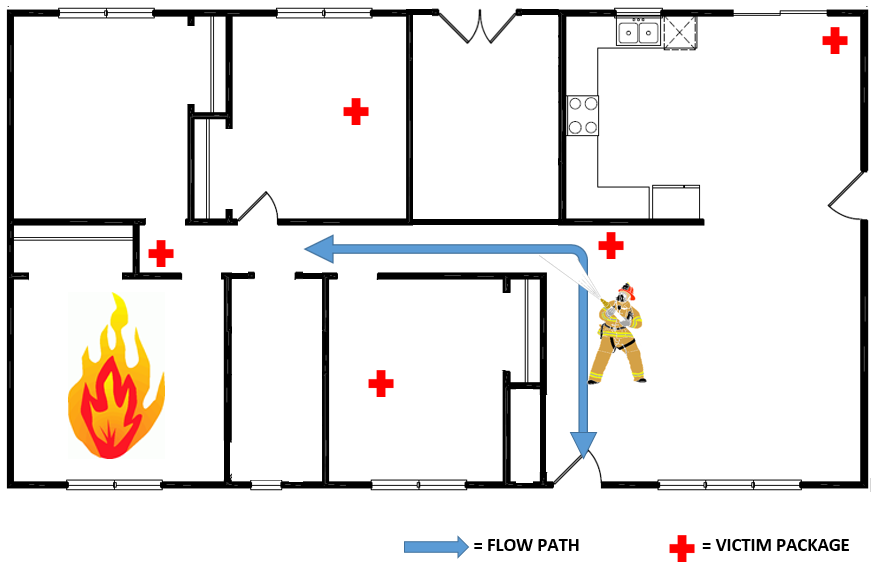
\includegraphics[width=5in]{Figures/General/No_Vent_interior_config}
	\caption{`No Vent' configuration used during Experiments~1--6.}
	\label{fig:No_Vent_int}
\end{figure}

\begin{table}[!ht]
\caption{Summary of Experiments~1--6}
\centering
\scalebox{0.75}{
\begin{tabular}{|c|c|c|c|c|l|}
\hline
\multirow{2}{*}{Experiment} 	& Fire Attack 	& \multirow{2}{*}{Nozzle}		& \multirow{2}{*}{Advancement} 		& \multirow{2}{*}{Pattern}		& \multicolumn{1}{c|}{\multirow{2}{*}{Ventilation Parameters}} \\ 
								& 	Method	   	& 								& 									& 								& 										\\ 
\hline \hline
\multirow{2}{*}{1}	& \multirow{2}{*}{Interior} & \multicolumn{3}{c|}{Delayed water application with combination;} 									& \multirow{2}{*}{Flow path between front door \& BR1 fire} \\
					& 							& \multicolumn{3}{c|}{Shutdown \& Move; Straight Stream} 											& 		\\
\hline 		
	2							& Interior  	& Smooth Bore 					& 	Flow \& Move 					&  Solid Stream 				& Flow path between front door \& BR1 fire 	\\
\hline
\multirow{2}{*}{3}	& \multirow{2}{*}{Interior} & \multirow{2}{*}{Smooth Bore} 	& \multirow{2}{*}{Shutdown \& Move}	& \multirow{2}{*}{Solid Stream} & Flow path between front door \& BR1 fire \\
					& 							& 								& 									& 								& ~~w/ door control 	\\
\hline
\multirow{2}{*}{4}	& \multirow{2}{*}{Interior} & \multirow{2}{*}{Smooth Bore} 	& \multirow{2}{*}{Flow \& Move} 	& \multirow{2}{*}{Solid Stream} & Flow path between front door \& BR1 fire 	\\
 					& 							& 								& 									& 								& ~~w/ coordinated horizontal vent 				\\
\hline
\multirow{2}{*}{5}	& \multirow{2}{*}{Interior} & \multirow{2}{*}{Combination} 	& \multirow{2}{*}{Shutdown \& Move} &  Narrow Fog, near to far 		& \multirow{2}{*}{Flow path between front door \& BR1 fire} \\
 					& 							& 								& 									&  along hall centerline		& 		\\
\hline
	6							& Interior 		& 	Smooth Bore 				& Shutdown \& Move 					&  Solid Stream 				& Flow path between front door \& BR1 fire 	\\
\hline
\end{tabular}}
\label{table:Exp1to6}
\end{table}

\FloatBarrier

\subsubsection{Experiment 1}
Experiment~1 looked at the fire dynamics in a typical single-story structure with delayed water application. The fire was ignited in Bedroom~1 and allowed to develop until it became ventilation limited. Then, the front door was opened to simulate fire department arrival. The open door established a flow path between itself and Bedroom~1. Once the fire reached steady state, suppression was performed via an interior attack through the front door with a combination nozzle on straight stream. The nozzle was shutdown as the hoseline advanced. Figure~\ref{fig:No_Vent_int} shows the configuration of the structure and Table~\ref{Table:Exp1Interventions} shows at what times interventions were performed. The results of Experiment 1 can be found in Appendix~\ref{App:Exp1Results}. 

%To view the full experiment video \href{https://player.vimeo.com/video/170499605?autoplay=1}{Click Here}.

\begin{table}[!ht]
	\centering
	\caption{Experiment 1 Interventions}
	\begin{tabular}{|c|c|} 
		\hline
		Time & Intervention \\ \hline \hline
		00:00 & Ignition --- Bedroom 1 \\ \hline
		08:17 & Front Door Open \\ \hline
		27:47 & Suppression Crew Enters\\ \hline
		27:54 & Hallway Suppression \\ \hline
		42:19 & End Experiment\\ \hline
	\end{tabular}
	\label{Table:Exp1Interventions}
\end{table}

\FloatBarrier

\subsubsection{Experiment 2}

Experiment~2 looked at the fire dynamics in a single-story structure when suppression is conducted with a smooth bore nozzle, flowing while moving. The fire was ignited in Bedroom~1 and allowed to develop until it reached steady state. Then, the front door was opened to simulate fire department arrival. The open door established a flow path between itself and Bedroom~1. An interior fire attack was initiated through the front door with a solid stream from a smooth bore nozzle. The nozzle continued to flow as the hoseline advanced. Figure~\ref{fig:No_Vent_int} shows the configuration of the structure and Table~\ref{Table:Exp2Interventions} shows at what times interventions were performed. The results of Experiment 2 can be found in Appendix~\ref{App:Exp2Results}. 

%To view the full experiment video \href{https://player.vimeo.com/video/170510934?autoplay=1}{Click Here}.

\begin{table}[!ht]
	\centering
	\caption{Experiment 2 Interventions}
	\begin{tabular}{|c|c|} 
		\hline
		Time & Intervention \\ \hline \hline
		00:00 & Ignition - Bedroom 1 \\ \hline
		07:05 & Front Door Open \\ \hline
		07:18 & Suppression Crew Enters\\ \hline
		07:23 & Burst Suppression \\ \hline 
		07:36 & Hallway Suppression \\ \hline
		18:02 & End Experiment\\ \hline
	\end{tabular}
	\label{Table:Exp2Interventions}
\end{table}

\FloatBarrier

\subsubsection{Experiment 3}
Experiment~3 looked at the fire dynamics in a single-story structure when suppression is conducted with a solid stream and the front door controlled immediately following entry. The fire was ignited in Bedroom~1 and allowed to develop until it became ventilation limited. Then, the front door was opened to simulate fire department arrival. The open door established a flow path between itself and Bedroom~1. An interior fire attack was initiated through the front door with a solid stream from a smooth bore nozzle. After the suppression crew entered, the door was closed to the width of the hoseline in an effort to limit the amount of fresh air supplied to the fire (Door Control). The nozzle was shutdown as the hoseline advanced. Figure~\ref{fig:No_Vent_int} shows the configuration of the structure and Table~\ref{Table:Exp3Interventions} shows at what times interventions were performed. The results of Experiment 3 can be found in Appendix~\ref{App:Exp3Results}.

%To view the full experiment video \href{https://player.vimeo.com/video/170513516?autoplay=1}{Click Here}.

\begin{table}[!ht]
	\centering
	\caption{Experiment 3 Interventions}
	\begin{tabular}{|c|c|} 
		\hline
		Time & Intervention \\ \hline \hline
		00:00 & Ignition - Bedroom 1 \\ \hline
		08:26 & Front Door Open \\ \hline
		08:28 & Suppression Crew Enters\\ \hline
		08:32 & Burst Suppression \\ \hline 
		08:45 & Hallway Suppression \\ \hline
		19:09 & End Experiment\\ \hline
	\end{tabular}
	\label{Table:Exp3Interventions}
\end{table}

\FloatBarrier

\subsubsection{Experiment 4}
Experiment~4 looked at the fire dynamics in a single-story structure when suppression is conducted with a smooth bore nozzle. The fire was ignited in Bedroom~1 and allowed to develop until it became ventilation limited. Then, the front door was opened to simulate fire department arrival. The open door established a flow path between itself and Bedroom~1. An interior fire attack was initiated through the front door with a solid stream from a smooth bore nozzle. The nozzle continued to flow as the hoseline advanced, and suppression was coordinated with horizontal ventilation of the Bedroom~1 window. Figure~\ref{fig:No_Vent_int} shows the configuration of the structure and Table~\ref{Table:Exp4Interventions} shows at what times interventions were performed. The results of Experiment 4 can be found in Appendix~\ref{App:Exp4Results}. 

%To view the full experiment video \href{https://player.vimeo.com/video/170499609?autoplay=1}{Click Here}.

\begin{table}[!ht]
	\centering
	\caption{Experiment 4 Interventions}
	\begin{tabular}{|c|c|} 
		\hline
		Time & Intervention \\ \hline \hline
		00:00 & Ignition - Bedroom 1 \\ \hline
		08:25 & Front Door Open \\ \hline
		08:38 & Suppression Crew Enters\\ \hline
		08:43 & Burst Suppression \\ \hline
		08:43 & Bedroom 1 Window Open \\ \hline 
		08:54 & Hallway Suppression \\ \hline
		15:23 & End Experiment\\ \hline
	\end{tabular}
	\label{Table:Exp4Interventions}
\end{table}

\FloatBarrier

\subsubsection{Experiment 5}
Experiment~5 looked at the fire dynamics in a single-story structure when suppression is conducted with a narrow fog from a combination nozzle. The fire was ignited in the Bedroom~1 and allowed to develop until it became ventilation limited. Then, the front door was opened to simulate fire department arrival. The open door established a flow path between itself and Bedroom~1. An interior fire attack was initiated through the front door with a narrow fog stream from a combination nozzle. The nozzle was shutdown as the hoseline advanced. Figure~\ref{fig:No_Vent_int} shows the configuration of the structure and Table~\ref{Table:Exp5Interventions} shows at what times interventions were performed. The results of Experiment~5 can be found in Appendix~\ref{App:Exp5Results}. 

%To view the full experiment video \href{https://player.vimeo.com/video/170511425?autoplay=1}{Click Here}.

\begin{table}[!ht]
	\centering
	\caption{Experiment 5 Interventions}
	\begin{tabular}{|c|c|} 
		\hline
		Time & Intervention \\ \hline \hline
		00:00 & Ignition - Bedroom 1 \\ \hline
		06:57 & Front Door Open \\ \hline
		07:09 & Suppression Crew Enters\\ \hline
		07:16 & Burst Suppression \\ \hline 
		07:27 & Hallway Suppression \\ \hline
		17:54 & End Experiment\\ \hline
	\end{tabular}
	\label{Table:Exp5Interventions}
\end{table}

\FloatBarrier
\clearpage

\subsubsection{Experiment 6}
Experiment~6 looked at the fire dynamics in a single-story structure when suppression is conducted with a solid stream from a smooth bore nozzle. The fire was ignited in Bedroom~1 and allowed to develop until it became ventilation limited. Then, the front door was opened to simulate fire department arrival. The open door established a flow path between itself and Bedroom~1. An interior fire attack was initiated through the front door with a solid stream from a smooth bore nozzle. The nozzle was shutdown as the hoseline advanced. Figure~\ref{fig:No_Vent_int} shows the configuration of the structure and Table~\ref{Table:Exp6Interventions} shows at what times interventions were performed. The results of Experiment~6 can be found in Appendix~\ref{App:Exp6Results}. 

%To view the full experiment video \href{https://player.vimeo.com/video/170510936?autoplay=1}{Click Here}.

\begin{table}[!ht]
	\centering
	\caption{Experiment 6 Interventions}
	\begin{tabular}{|c|c|} 
		\hline
		Time & Intervention \\ \hline \hline
		00:00 & Ignition - Bedroom 1 \\ \hline
		07:58 & Front Door Open \\ \hline
		08:13 & Suppression Crew Enters\\ \hline
		08:18 & Burst Suppression \\ \hline 
		08:27 & Hallway Suppression \\ \hline
		14:38 & End Experiment\\ \hline
	\end{tabular}
	\label{Table:Exp6Interventions}
\end{table}

\clearpage

\subsection{Single Room --- Single Vent}
During Experiments~7--12, an interior suppression tactic was performed to extinguish a fire in the `Single Vent' configuration. This configuration, presented in Figure~\ref{fig:Single_Vent_int}, consisted of a fire in Bedroom~1 with the Bedroom~1 window open and all other vents initially closed. Specific details about the ventilation patterns and the type of interior fire attack method used during Experiments~7--12 are listed in Table~\ref{table:Exp7to12}. Following the table, a brief description of each experiment is provided along with a table of interventions and times at which they were performed during the experiment. 

\begin{figure}[!ht]
	\centering
	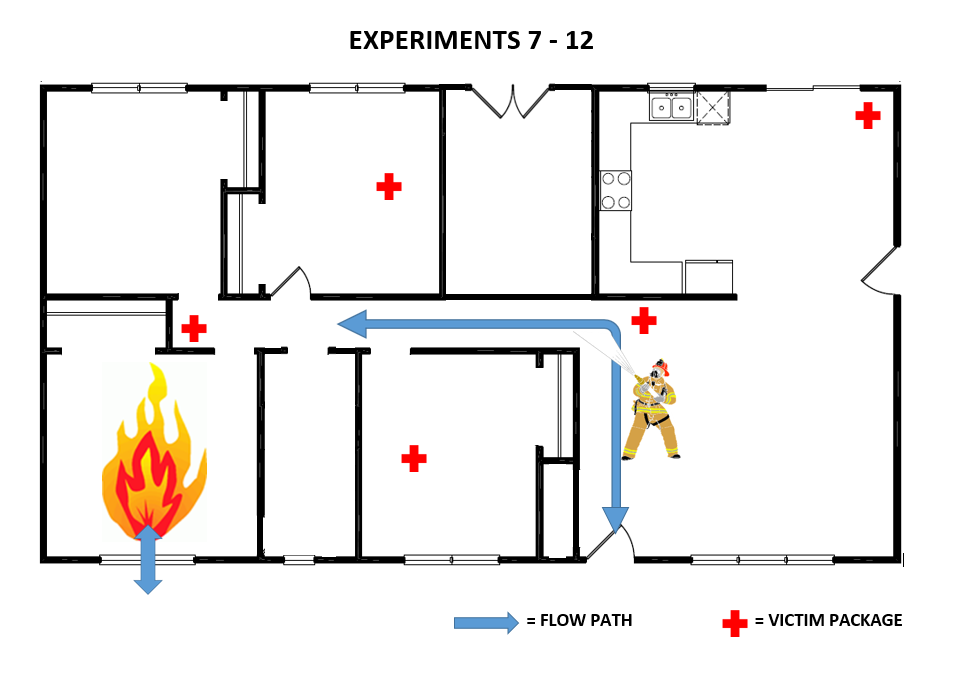
\includegraphics[width=5in]{Figures/General/Exps7through12.png}
	\caption{Configurations for Experiments 7 to 12}
	\label{fig:Single_Vent_int}
\end{figure}

\begin{table}[!ht]
\caption{Experiments 7 through 12}
\centering
\scalebox{0.75}{
\begin{tabular}{|c|c|c|c|c|l|}
\hline
\multirow{2}{*}{Experiment} 	& Fire Attack 	& \multirow{2}{*}{Nozzle}		& \multirow{2}{*}{Advancement} 		& \multirow{2}{*}{Pattern}	& \multicolumn{1}{c|}{\multirow{2}{*}{Ventilation Parameters}} \\ 
								& 	Method	   	& 								& 									& 									& 										\\ 
\hline \hline
\multirow{2}{*}{7}	& \multirow{2}{*}{Interior} & \multirow{2}{*}{Smooth Bore} 	& \multirow{2}{*}{Flow \& Move}		& \multirow{2}{*}{Solid Stream} 	& Flow paths between front door \& BR1 fire; \\
					& 							& 								& 									& 									& ~~BR1 fire \& BR1 window 	\\
\hline
\multirow{2}{*}{8}	& \multirow{2}{*}{Interior} & \multirow{2}{*}{Smooth Bore} 	& \multirow{2}{*}{Shutdown \& Move}	& \multirow{2}{*}{Solid Stream} 	& Flow paths between front door \& BR1 fire; 	\\
 					& 							& 								& 									& 									& ~~BR1 fire \& BR1 window 	\\
\hline
\multirow{2}{*}{9}	& \multirow{2}{*}{Interior} & \multirow{2}{*}{Combination} 	& \multirow{2}{*}{Flow \& Move}		& \multirow{2}{*}{Straight Stream} 	& Flow paths between front door \& BR1 fire; \\
					& 							& 								& 									& 									& ~~BR1 fire \& BR1 window 	\\
\hline
\multirow{2}{*}{10}	& \multirow{2}{*}{Interior} & \multirow{2}{*}{Combination} 	& \multirow{2}{*}{Shutdown \& Move}	& \multirow{2}{*}{Straight Stream} 	& Flow paths between front door \& BR1 fire; 	\\
 					& 							& 								& 									& 									& ~~BR1 fire \& BR1 window 	\\
\hline
\multirow{2}{*}{11}	& \multirow{2}{*}{Interior} & \multirow{2}{*}{Combination} 	& \multirow{2}{*}{Flow \& Move} 	&  \multirow{2}{*}{Narrow Fog} 		& Flow paths between front door \& BR1 fire; 	\\
 					& 							& 								& 									&  									& ~~BR1 fire \& BR1 window 	\\
\hline
\multirow{2}{*}{12}	& \multirow{2}{*}{Interior} & \multicolumn{3}{c|}{Delayed water application w/ Combination;} 										& Flow paths between front door \& BR1 fire; 	\\
					& 							& \multicolumn{3}{c|}{Flow \& Move; Straight Stream} 													& ~~BR1 fire \& BR1 window 	\\
\hline
\end{tabular}}
\label{table:Exp7to12}
\end{table}

\FloatBarrier

\subsubsection{Experiment 7}
Experiment~7 looked at the fire dynamics in a single-story structure where suppression was conducted with a solid stream. The fire was ignited in the Bedroom~1 with the Bedroom~1 window open. The fire develops and becomes ventilation limited. Once this happens, the front door was opened, simulating fire department arrival and establishing two flow paths; One between the front door and the bedroom fire and the other between the bedroom window and the bedroom fire. An interior fire attack was initiated through the front door, utilizing a solid stream from a smooth bore nozzle. The nozzle was flowing as the hoseline advanced. Figure~\ref{fig:Single_Vent_int} shows the configuration of the structure and Table~\ref{Table:Exp7Interventions} shows at what times interventions were performed. The results of Experiment~7 can be found in Appendix~\ref{App:Exp7Results}. 

%To view the full experiment video \href{https://player.vimeo.com/video/170513517?autoplay=1}{Click Here}.

\begin{table}[H]
	\centering
	\caption{Experiment 7 Interventions}
	\begin{tabular}{|c|c|} 
		\hline
		Time & Intervention \\ \hline \hline
		00:00 & Ignition - Bedroom \\ \hline
		05:55 & Front Door Open \\ \hline
		06:07 & Suppression Crew Enters\\ \hline
		06:12 & Burst Suppression \\ \hline 
		06:22 & Hallway Suppression \\ \hline
		12:26 & End Experiment\\ \hline
	\end{tabular}
	\label{Table:Exp7Interventions}
\end{table}

\FloatBarrier

\subsubsection{Experiment 8}
Experiment~8 looked at the fire dynamics in a single-story structure where suppression was conducted with a solid stream. The fire was ignited in the Bedroom~1 with the Bedroom~1 window open. The fire develops and becomes ventilation limited. Once this happens, the front door was opened, simulating fire department arrival and establishing two flow paths; One between the front door and the bedroom fire and the other between the bedroom window and the bedroom fire. An interior fire attack was initiated through the front door, utilizing a solid stream from a smooth bore nozzle. The nozzle shutdown while the hoseline advanced. Figure~\ref{fig:Single_Vent_int} shows the configuration of the structure and Table~\ref{Table:Exp8Interventions} shows at what times interventions were performed. The results of Experiment~8 can be found in Appendix~\ref{App:Exp8Results}. 

%To view the full experiment video \href{https://player.vimeo.com/video/170499608?autoplay=1}{Click Here}.

\begin{table}[H]
	\centering
	\caption{Experiment 8 Interventions}
	\begin{tabular}{|c|c|} 
		\hline
		Time & Intervention \\ \hline \hline
		00:00 & Ignition - Bedroom \\ \hline
		05:26 & Front Door Open \\ \hline
		05:40 & Suppression Crew Enters\\ \hline
		05:45 & Burst Suppression \\ \hline 
		05:54 & Hallway Suppression \\ \hline
		11:57 & End Experiment\\ \hline
	\end{tabular}
	\label{Table:Exp8Interventions}
\end{table}

\FloatBarrier

\subsubsection{Experiment 9}
Experiment~9 looked at the fire dynamics in a single-story structure where suppression was conducted with a straight stream pattern from a combination nozzle. The fire was ignited in the Bedroom~1 with the Bedroom~1 window open. The fire develops and becomes ventilation limited. Once this happens, the front door was opened, simulating fire department arrival and establishing two flow paths; one between the front door and the bedroom fire and the other between the bedroom window and the bedroom fire. An interior fire attack was initiated through the front door, utilizing a straight stream from a combination nozzle. The nozzle was flowing while the hoseline was advanced. Figure~\ref{fig:Single_Vent_int} shows the configuration of the structure and Table~\ref{Table:Exp9Interventions} shows at what times interventions were performed. The results of Experiment~9 can be found in Appendix~\ref{App:Exp9Results}. 

%To view the full experiment video \href{https://player.vimeo.com/video/170510938?autoplay=1}{Click Here}.

\begin{table}[H]
	\centering
	\caption{Experiment 9 Interventions}
	\begin{tabular}{|c|c|} 
		\hline
		Time & Intervention \\ \hline \hline
		00:00 & Ignition - Bedroom \\ \hline
		05:27 & Front Door Open \\ \hline
		05:38 & Suppression Crew Enters\\ \hline
		05:45 & Burst Suppression \\ \hline 
		05:53 & Hallway Suppression \\ \hline
		11:59 & End Experiment\\ \hline
	\end{tabular}
	\label{Table:Exp9Interventions}
\end{table}

\FloatBarrier

\subsubsection{Experiment 10}
Experiment~10 looked at examine the fire dynamics in a single-story structure where suppression was conducted with a straight stream. The fire was ignited in the Bedroom~1 with the Bedroom~1 window open. The fire develops and becomes ventilation limited. Once this happens, the front door was opened, simulating fire department arrival and establishing two flow paths; one between the front door and the bedroom fire and the other between the bedroom window and the bedroom fire. An interior fire attack was initiated through the front door, utilizing a straight stream from a combination nozzle. The nozzle was shutdown while the hoseline advanced. Figure~\ref{fig:Single_Vent_int} shows the configuration of the structure and Table~\ref{Table:Exp10Interventions} shows at what times interventions were performed. The results of Experiment~10 can be found in Appendix~\ref{App:Exp10Results}. 

%To view the full experiment video \href{https://player.vimeo.com/video/170510939?autoplay=1}{Click Here}.

\begin{table}[H]
	\centering
	\caption{Experiment 10 Interventions}
	\begin{tabular}{|c|c|} 
		\hline
		Time & Intervention \\ \hline \hline
		00:00 & Ignition - Bedroom \\ \hline
		05:27 & Front Door Open \\ \hline
		05:39 & Suppression Crew Enters\\ \hline
		05:45 & Burst Suppression \\ \hline 
		05:54 & Hallway Suppression \\ \hline
		12:07 & End Experiment\\ \hline
	\end{tabular}
	\label{Table:Exp10Interventions}
\end{table}

\FloatBarrier

\subsubsection{Experiment 11}
Experiment~11 looked at the fire dynamics in a single-story structure where suppression was conducted with a fog stream pattern from a combination nozzle. The fire was ignited in Bedroom~1 with the Bedroom~1 window open. The fire develops and becomes ventilation limited. Once this happens, the front door was opened, simulating fire department arrival and establishing two flow paths; one between the front door and the bedroom fire and the other between the bedroom window and the bedroom fire. An interior fire attack was initiated through the front door, utilizing a narrow fog stream from a combination nozzle. The nozzle was flowing while the hoseline advanced.  Figure~\ref{fig:Single_Vent_int} shows the configuration of the structure and Table~\ref{Table:Exp11Interventions} shows at what times interventions were performed. The results of Experiment 11 can be found in Appendix~\ref{App:Exp11Results}. 

%To view the full experiment video \href{https://player.vimeo.com/video/170499614?autoplay=1}{Click Here}.

\begin{table}[H]
	\centering
	\caption{Experiment 11 Interventions}
	\begin{tabular}{|c|c|} 
		\hline
		Time & Intervention \\ \hline \hline
		00:00 & Ignition - Bedroom \\ \hline
		06:20 & Front Door Open \\ \hline
		06:32 & Suppression Crew Enters\\ \hline
		06:38 & Burst Suppression \\ \hline 
		06:49 & Hallway Suppression \\ \hline
		12:24 & End Experiment\\ \hline
	\end{tabular}
	\label{Table:Exp11Interventions}
\end{table}

\FloatBarrier

\subsubsection{Experiment 12}
Experiment~12 looked at the fire dynamics in a typical single-story structure with delayed water application. The fire was ignited in Bedroom~1 with the Bedroom~1 window open. Once the fire reaches steady state, the front door was opened, simulating fire department arrival. This establishes two flow paths; one between the front door and bedroom window and another between the bedroom window and the bedroom. Once the fire reaches steady state again the suppression was initiated via an interior suppression tactic with a combination nozzle set to straight stream. The water flow will be shutdown while the hoseline was moving.  Figure~\ref{fig:Single_Vent_int} shows the configuration of the structure and Table~\ref{Table:Exp12Interventions} shows at what times interventions were performed. The results of Experiment 12 can be found in Appendix~\ref{App:Exp12Results}. 
%To view the full experiment video \href{https://player.vimeo.com/video/170510940?autoplay=1}{Click Here}.

\begin{table}[H]
	\centering
	\caption{Experiment 12 Interventions}
	\begin{tabular}{|c|c|} 
		\hline
		Time & Intervention \\ \hline \hline
		00:00 & Ignition - Bedroom 1 \\ \hline
		05:57 & Front Door Open \\ \hline
		13:29 & Suppression Crew Enters\\ \hline
		13:32 & Burst Suppression \\ \hline 
		13:40 & Hallway Suppression \\ \hline
		28:46 & End Experiment\\ \hline
	\end{tabular}
	\label{Table:Exp12Interventions}
\end{table}

\clearpage

\subsection{Two Room --- Two Vent}

During Experiments~13--17, an interior suppression tactic was performed to extinguish a fire in the `Two Vent' configuration. This configuration, presented in Figure~\ref{fig:Two_Vent_int}, consisted of a fire in Bedroom~1 with the Bedroom~1 window open, a fire in Bedroom~2 with the Bedroom~2 window open and all other vents initially closed. Specific details about the ventilation patterns and the type of interior fire attack method used during Experiments~13--17 are listed in Table~\ref{table:Exp13to17}. Following the table, a brief description of each experiment is provided along with a table of interventions and times at which they were performed during the experiment. 


\begin{figure}[!ht]
	\centering
	\includegraphics[width=5in]{Figures/General/Exps13through17.png}
	\caption{Configurations for Experiments 13 to 17}
	\label{fig:Two_Vent_int}
\end{figure}

\begin{table}[!ht]
\caption{Experiments 13 through 17}
\centering
\scalebox{0.75}{
\begin{tabular}{|c|c|c|c|c|l|}
\hline
\multirow{2}{*}{Experiment} 	& Fire Attack 	& \multirow{2}{*}{Nozzle}		& \multirow{2}{*}{Advancement} 		& \multirow{2}{*}{Pattern}	& \multicolumn{1}{c|}{\multirow{2}{*}{Ventilation Parameters}} \\ 
								& 	Method	   	& 								& 									& 									& 										\\ 
\hline \hline
\multirow{3}{*}{13}	& \multirow{3}{*}{Interior} & \multirow{3}{*}{Smooth Bore} 	& \multirow{3}{*}{Flow \& Move}		& \multirow{3}{*}{Solid Stream} 	& Flow paths between front door \& BR1 fire; BR1 fire \\
					& 							& 								& 									& 									& ~~\& BR1 window; front door \& BR2 fire; BR2 fire	\\
					& 							& 								& 									& 									& ~~\& BR2 window \\
\hline
\multirow{3}{*}{14}	& \multirow{3}{*}{Interior} & \multirow{3}{*}{Smooth Bore} 	& \multirow{3}{*}{Shutdown \& Move}	& \multirow{3}{*}{Solid Stream} 	& Flow paths between front door \& BR1 fire; BR1 fire \\
					& 							& 								& 									& 									& ~~\& BR1 window; front door \& BR2 fire; BR2 fire	\\
					& 							& 								& 									& 									& ~~\& BR2 window \\
\hline
\multirow{3}{*}{15}	& \multirow{3}{*}{Interior} & \multirow{3}{*}{Smooth Bore} 	& \multirow{3}{*}{Shutdown \& Move}	& \multirow{3}{*}{Solid Stream} 	& Flow paths between front door \& BR1 fire; BR1 fire \\
					& 							& 								& 									& 									& ~~\& BR1 window; front door \& BR2 fire; BR2 fire	\\
					& 							& 								& 									& 									& ~~\& BR2 window w/ door control \\
\hline
\multirow{3}{*}{16}	& \multirow{3}{*}{Interior} & \multirow{3}{*}{Combination} 	& \multirow{3}{*}{Flow \& Move}		& \multirow{3}{*}{Narrow Fog} 		& Flow paths between front door \& BR1 fire; BR1 fire \\
					& 							& 								& 									& 									& ~~\& BR1 window; front door \& BR2 fire; BR2 fire	\\
					& 							& 								& 									& 									& ~~\& BR2 window \\
\hline
\multirow{3}{*}{17}	& \multirow{3}{*}{Interior} & \multicolumn{3}{c|}{Delayed water application w/}														& Flow paths between front door \& BR1 fire; BR1 fire \\
					& 							& \multicolumn{3}{c|}{Combination; Flow \& Move;}														& ~~\& BR1 window; front door \& BR2 fire; BR2 fire	\\
					& 							& \multicolumn{3}{c|}{Straight Stream}																	& ~~\& BR2 window \\
\hline
\end{tabular}}
\label{table:Exp13to17}
\end{table}

\FloatBarrier

\subsubsection{Experiment 13}
Experiment~13 looked at the fire dynamics of a 2-bedroom fire in a single-story structure where suppression was conducted with a solid stream pattern. The fire was ignited simultaneously in Bedroom~1 and Bedroom~2 with the Bedroom~1 and Bedroom~2 windows open. The fire develops and becomes ventilation limited. Once this happens, the front door was opened, simulating fire department arrival. These actions create flow paths between the front door and each fire bedroom and between each bedroom window and the fire bedrooms. An interior fire attack was initiated through the front door, utilizing a solid stream from a smooth bore nozzle. The nozzle was flowing while the hoseline advanced. Figure~\ref{fig:Two_Vent_int} shows the configuration of the structure and Table~\ref{Table:Exp13Interventions} shows at what times interventions were performed. The results of Experiment~13 can be found in Appendix~\ref{App:Exp13Results}. 

%To view the full experiment video \href{https://player.vimeo.com/video/170499618?autoplay=1}{Click Here}.

\begin{table}[H]
	\centering
	\caption{Experiment 13 Interventions}
	\begin{tabular}{|c|c|} 
		\hline
		Time & Intervention \\ \hline \hline
		00:00 & Ignition - Bedroom 1 \& 2 \\ \hline
		05:39 & Front Door Open \\ \hline
		05:52 & Suppression Crew Enters\\ \hline
		05:57 & Burst Suppression \\ \hline 
		06:11 & Hallway Suppression \\ \hline
		12:06 & End Experiment\\ \hline
	\end{tabular}
	\label{Table:Exp13Interventions}
\end{table}

\FloatBarrier

\subsubsection{Experiment 14}
Experiment~14 looked at the fire dynamics of a 2-bedroom fire in a single-story structure where suppression was conducted with a solid stream from a combination nozzle. The fire was ignited simultaneously in the Bedroom~1 and Bedroom~2 with the Bedroom~1 and Bedroom~2 windows open. The fire develops and becomes ventilation limited. Once this happens, the front door was opened simulating fire department arrival. These actions create flow paths between the front door and each fire bedroom and between each bedroom window and the fire bedrooms. An interior fire attack was initiated through the front door, utilizing a solid stream from a combination nozzle. The nozzle was shutdown while the hoseline advanced. Figure~\ref{fig:Two_Vent_int} shows the configuration of the structure and Table~\ref{Table:Exp14Interventions} shows at what times interventions were performed. The results of Experiment~14 can be found in Appendix~\ref{App:Exp14Results}. 

%To view the full experiment video \href{https://player.vimeo.com/video/170499611?autoplay=1}{Click Here}.

\begin{table}[H]
	\centering
	\caption{Experiment 14 Interventions}
	\begin{tabular}{|c|c|} 
		\hline
		Time & Intervention \\ \hline \hline
		00:00 & Ignition - Bedroom 1 \& 2 \\ \hline
		06:26 & Front Door Open \\ \hline
		06:39 & Suppression Crew Enters\\ \hline
		06:43 & Burst Suppression \\ \hline 
		06:50 & Hallway Suppression \\ \hline
		15:05 & End Experiment\\ \hline
	\end{tabular}
	\label{Table:Exp14Interventions}
\end{table}

\FloatBarrier

\subsubsection{Experiment 15}
Experiment~15 looked at the fire dynamics of a 2-bedroom fire in a single-story structure where suppression was conducted with a solid stream pattern. The fire is ignited simultaneously in Bedroom~1 and Bedroom~2 with the Bedroom~1 and Bedroom~2 windows open. The fire develops and becomes ventilation limited. Once this happens, the front door was opened simulating fire department arrival. This action creates flow paths between the front door and each fire bedroom and between each bedroom window and the fire bedrooms. An interior fire attack was initiated through the front door, utilizing a solid stream from a smooth bore nozzle. After the suppression crew enters, the door was closed to the width of the hoseline in an effort to limit the amount of fresh air supplied to the fire (Door Control). The nozzle was shutdown while the hoseline advanced. Figure~\ref{fig:Two_Vent_int} shows the configuration of the structure and Table~\ref{Table:Exp15Interventions} shows at what times interventions were performed. The results of Experiment~15 can be found in Appendix~\ref{App:Exp15Results}. 

%To view the full experiment video \href{https://player.vimeo.com/video/170499619?autoplay=1}{Click Here}.

\begin{table}[H]
	\centering
	\caption{Experiment 15 Interventions}
	\begin{tabular}{|c|c|} 
		\hline
		Time & Intervention \\ \hline \hline
		00:00 & Ignition - Bedroom 1 \& 2 \\ \hline
		05:39 & Front Door Open \\ \hline
		05:40 & Suppression Crew Enters\\ \hline
		05:44 & Burst Suppression \\ \hline 
		05:55 & Hallway Suppression \\ \hline
		12:06 & End Experiment\\ \hline
	\end{tabular}
	\label{Table:Exp15Interventions}
\end{table}

\FloatBarrier

\paragraph{Experiment 16}
Experiment~16 looked at the fire dynamics of a 2-bedroom fire in a single-story structure where suppression was conducted with a narrow fog stream. The fire was ignited simultaneously in Bedroom~1 and Bedroom~2 with the Bedroom~1 and Bedroom~2 windows open. The fire develops and becomes ventilation limited. Once this happens, the front door was opened simulating fire department arrival. These actions create flow paths between the front door and each fire bedroom and between each bedroom window and the fire bedrooms. An interior fire attack was initiated through the front door, utilizing a narrow fog stream from a combination nozzle. The nozzle was flowing while the hoseline advanced. Figure~\ref{fig:Two_Vent_int} shows the configuration of the structure and Table~\ref{Table:Exp16Interventions} shows at what times interventions were performed. The results of Experiment~16 can be found in Appendix~\ref{App:Exp16Results}. 

%To view the full experiment video \href{https://player.vimeo.com/video/170510941?autoplay=1}{Click Here}.

\begin{table}[H]
	\centering
	\caption{Experiment 16 Interventions}
	\begin{tabular}{|c|c|} 
		\hline
		Time & Intervention \\ \hline \hline
		00:00 & Ignition - Bedroom 1 \& 2 \\ \hline
		05:23 & Front Door Open \\ \hline
		05:33 & Suppression Crew Enters\\ \hline
		05:37 & Burst Suppression \\ \hline 
		05:54 & Hallway Suppression \\ \hline
		11:45 & End Experiment\\ \hline
	\end{tabular}
	\label{Table:Exp16Interventions}
\end{table}

\FloatBarrier

\paragraph{Experiment 17}
Experiment~17 looked at the fire dynamics of a 2-bedroom fire in a single-story structure where suppression was conducted with delayed suppression. The fire was ignited simultaneously in Bedroom~1 and Bedroom~2 with the Bedroom~1 and Bedroom~2 windows open. The fire develops and becomes ventilation limited. Once this happens, the front door was opened, simulating fire department arrival. These actions create flow paths between the front door and each fire bedroom and between each bedroom window and the fire bedrooms. An interior fire attack was initiated through the front door, utilizing a stream from a combination nozzle. The nozzle was shutdown while the hoseline advanced Figure~\ref{fig:Two_Vent_int} shows the configuration of the structure and Table~\ref{Table:Exp17Interventions} shows at what times interventions were performed. The results of Experiment~17 can be found in Appendix~\ref{App:Exp17Results}. 

%To view the full experiment video \href{https://player.vimeo.com/video/170499615?autoplay=1}{Click Here}.

\begin{table}[H]
	\centering
	\caption{Experiment 17 Interventions}
	\begin{tabular}{|c|c|} 
		\hline
		Time & Intervention \\ \hline \hline
		00:00 & Ignition - Bedroom 1 \& 2 \\ \hline
		05:27 & Front Door Open \\ \hline
		10:32 & Suppression Crew Enters\\ \hline
		10:36 & Burst Suppression \\ \hline 
		10:47 & Hallway Suppression \\ \hline
		23:32 & End Experiment\\ \hline
	\end{tabular}
	\label{Table:Exp17Interventions}
\end{table}

\clearpage

\section{Transitional}

\subsection{Single Room --- Single Vent}
During Experiments~18--20, a transitional attack was performed to extinguish a fire in the `Single Vent' configuration. This configuration, presented in Figure~\ref{fig:Single_Vent_ext}, consisted of a fire in Bedroom~1 with the Bedroom~1 window open and all other vents initially closed. Specific details about the ventilation patterns and the type of transitional fire attack method used during Experiments~18--20 are listed in Table~\ref{table:Exp18to20}. 

\begin{figure}[H]
	\centering
	\includegraphics[width=5in]{Figures/General/Exps18through20.png}
	\caption{Configuration for Experiments 18 through 20.}
	\label{fig:Single_Vent_ext}
\end{figure}

\begin{table}[H]
\caption{Experiments 18 through 20}
\centering
\scalebox{0.75}{
\begin{tabular}{|c|c|c|c|c|l|}
\hline
\multirow{2}{*}{Experiment} 	& Fire Attack 	& \multirow{2}{*}{Nozzle}	& \multirow{2}{*}{Advancement} 	& \multirow{2}{*}{Pattern}	& \multirow{2}{*}{Ventilation Parameters} \\ 
								& 	Method	   	& 							& 								& 							& 										\\ 
\hline \hline
18 					& Exterior 					& 	Smooth bore 				& Steep angle 				& 	Solid stream 			& 	Flow path between BR1 fire \& BR1 window \\
\hline
					&  							& 								& Occlude opening, 		 	&  	Narrow fog, rebuild, 		& 	\\
 		19			& 			Exterior		& 	Combination					& rebuild, steep angle   	&  	straight stream to  		& 	Flow path between BR1 fire \& BR1 window		\\
 					& 							& 								& to fog whip				& 	fog whip 					& 		\\
\hline
\multirow{2}{*}{20}	& \multirow{2}{*}{Exterior} & \multirow{2}{*}{Smooth bore} 	& Steep angle to 			&  	Solid stream to 	& 	\multirow{2}{*}{Flow path between BR1 fire \& BR1 window} 	\\
 					& 							& 								& half bale whip  			&  	half bale whip 		& 			\\
\hline
\end{tabular}}
\label{table:Exp18to20}
\end{table}

\FloatBarrier

During Experiment~21, a transitional attack was performed to extinguish a fire in the `Single Vent' configuration. This configuration, presented in Figure~\ref{fig:Single_Vent_ext_alt1}, consisted of a fire in Bedroom~1 with the Bedroom~1 window and front door open, all other vents were initially closed. Specific details about the ventilation patterns and the type of transitional fire attack method used during Experiment~21 are listed in Table~\ref{table:Exp21}.

\begin{figure}[H]
	\centering
	\includegraphics[width=5in]{Figures/General/Exp21.png}
	\caption{Configuration for Experiment 21.}
	\label{fig:Single_Vent_ext_alt1}
\end{figure}

\begin{table}[H]
\caption{Experiment 21}
\centering
\scalebox{0.75}{
\begin{tabular}{|c|c|c|c|c|l|}
\hline
\multirow{2}{*}{Experiment} 	& Fire Attack 	& \multirow{2}{*}{Nozzle}	& \multirow{2}{*}{Advancement} 	& \multirow{2}{*}{Pattern}	& \multirow{2}{*}{Ventilation Parameters} \\ 
								& 	Method	   	& 							& 								& 							& 										\\ 
\hline \hline
\multirow{2}{*}{21}	& \multirow{2}{*}{Exterior} & \multirow{2}{*}{Smooth bore} 	& Steep angle to 			&  Solid stream to 		& Flow paths between front door \& BR1 fire; 	\\
 					& 							& 								& half bale whip			&  half bale whip		& ~~BR1 fire \& BR1 window \\
\hline
\end{tabular}}
\label{table:Exp21}
\end{table}

During Experiment~26, a transitional attack was performed to extinguish a fire in the `Single Vent' configuration. This configuration, presented in Figure~\ref{fig:Single_Vent_ext_alt2}, consisted of a fire in Bedroom~4 with the Bedroom~4 window open and all other vents initially closed. Specific details about the ventilation patterns and the type of transitional fire attack method used during Experiment~26 are listed in Table~\ref{table:Exp26}.


\begin{figure}[H]
	\centering
	\includegraphics[width=5in]{Figures/General/Exp27.png}
	\caption{Configuration for Experiment 27.}
	\label{fig:Single_Vent_ext_alt2}
\end{figure}

\begin{table}[H]
\caption{Experiment 26}
\centering
\scalebox{0.75}{
\begin{tabular}{|c|c|c|c|c|l|}
\hline
\multirow{2}{*}{Experiment} 	& Fire Attack 	& \multirow{2}{*}{Nozzle}	& \multirow{2}{*}{Advancement} 	& \multirow{2}{*}{Pattern}	& \multirow{2}{*}{Ventilation Parameters} \\ 
								& 	Method	   	& 							& 								& 							& 										\\ 
\hline \hline
\multirow{2}{*}{26}	& \multirow{2}{*}{Exterior} & \multirow{2}{*}{Combination} 	& \multirow{2}{*}{Steep angle sweep} &  \multirow{2}{*}{Straight stream} & Flow paths between front door \& BR4 fire; 	\\
 					& 							& 								& 							&  						& ~~BR4 fire \& BR4 window 	\\
\hline
\end{tabular}}
\label{table:Exp26}
\end{table}

The following sections contain a brief description of each experiment along with a table of interventions and times at which they were performed during each experiment. 

\FloatBarrier

\subsubsection{Experiment 18}
Experiment~18 looked at the fire dynamics of a bedroom fire in a single-story structure where suppression was initiated from the exterior of the house. The fire was ignited in Bedroom~1. The fire develops and becomes ventilation limited. Once this happens a transitional attack was initiated starting at the Bedroom~1 window via a straight stream from a combination nozzle.  The suppression crew then transitioned to the interior for final suppression. The crew used a burst suppression the check conditions then proceeded directly to the fire room. Figure~\ref{fig:Single_Vent_ext} shows the configuration of the structure and Table~\ref{Table:Exp18Interventions} shows at what times interventions were performed. The results of Experiment~18 can be found in Appendix~\ref{App:Exp18Results}. 

%To view the full experiment video \href{https://player.vimeo.com/video/170499622?autoplay=1}{Click Here}.

\begin{table}[H]
	\centering
	\caption{Experiment 18 Interventions}
	\begin{tabular}{|c|c|} 
		\hline
		Time & Intervention \\ \hline \hline
		00:00 & Ignition - Bedroom 1 \\ \hline
		05:24 & Exterior Suppression BR1 Window Solid Stream \\ \hline
		05:35 & Front Door Open \\ \hline
		05:42 & Suppression Crew Enters\\ \hline
		05:45 & Burst Suppression \\ \hline 
		06:07 & Room Suppression \\ \hline
		12:04 & End Experiment\\ \hline
	\end{tabular}
	\label{Table:Exp18Interventions}
\end{table}

\FloatBarrier

\subsubsection{Experiment 19}
Experiment~19 looked at the fire dynamics of a bedroom fire in a single-story structure where suppression was initiated from the exterior. The fire was ignited in Bedroom~1. The fire develops and becomes ventilation limited. Once this happens a exterior water application was initiated through the Bedroom~1 window via a narrow fog stream from a combination nozzle. The fire was knocked back. The nozzle was shut down and the fire was permitted to regrow to the earlier ventilation limited state.  Once this happens a transitional fire attack was initiated starting at the Bedroom~1 window via a straight stream from a combination nozzle. The suppression crew then transitioned to the interior for final suppression. The crew entered the structure and proceeded directly to the fire room before flowing additional water. Figure~\ref{fig:Single_Vent_ext} shows the configuration of the structure and Table~\ref{Table:Exp19Interventions} shows at what times interventions were performed. The results of Experiment~19 can be found in Appendix~\ref{App:Exp19Results}. 

%To view the full experiment video \href{https://player.vimeo.com/video/170499621?autoplay=1}{Click Here}.

\begin{table}[H]
	\centering
	\caption{Experiment 19 Interventions}
	\begin{tabular}{|c|c|} 
		\hline
		Time & Intervention \\ \hline \hline
		00:00 & Ignition - Bedroom 1 \\ \hline
		05:24 & Exterior Suppression BR1 Window Narrow Fog Stream \\ \hline
		08:28 & Exterior Suppression BR1 Window Straight Stream \\ \hline
		08:58 & Front Door Open \\ \hline
		09:10 & Suppression Crew Enters\\ \hline
		09:34 & Room Suppression \\ \hline 
		14:05 & End Experiment\\ \hline
	\end{tabular}
	\label{Table:Exp19Interventions}
\end{table}

\FloatBarrier

\subsubsection{Experiment 20}
Experiments~20 looked at the fire dynamics of a bedroom fire in a single-story structure where suppression was initiated from the exterior of the house. The fire was ignited in Bedroom~1. The fire develops and becomes ventilation limited. Once this happens a transitional fire attack was initiated starting at the Bedroom~1 window via a solid stream from a smooth bore nozzle. After the initial application the suppression crew approaches the window, placed the nozzle through the window and opens the bale half way while making an `O' pattern. The nozzle was shutdown and the suppression crew, transitioned to the interior for final suppression. The crew entered the structure and proceeded directly to the fire room before flowing additional water. Figure~\ref{fig:Single_Vent_ext} shows the configuration of the structure and Table~\ref{Table:Exp20Interventions} shows at what times interventions were performed. The results of Experiment~20 can be found in Appendix~\ref{App:Exp20Results}. 

%To view the full experiment video \href{https://player.vimeo.com/video/170499620?autoplay=1}{Click Here}.

\begin{table}[H]
	\centering
	\caption{Experiment 20 Interventions}
	\begin{tabular}{|c|c|} 
		\hline
		Time & Intervention \\ \hline \hline
		00:00 & Ignition - Bedroom 1 \\ \hline
		06:52 & Exterior Suppression BR1 Window Solid Stream \\ \hline
		07:24 & Front Door Open \\ \hline
		07:34 & Suppression Crew Enters\\ \hline
		08:34 & Room Suppression \\ \hline 
		12:06 & End Experiment\\ \hline
	\end{tabular}
	\label{Table:Exp20Interventions}
\end{table}

\FloatBarrier

\subsubsection{Experiment 21}
Experiment~21 looked at the fire dynamics of a bedroom fire in a single-story structure where suppression was initiated from the exterior. The fire was ignited in Bedroom~1. The fire develops and becomes ventilation limited. Once this happens the front door was opened simulating an uncoordinated crew entry during a transitional fire attack. This action creates two flow paths; one between the front door and the bedroom and a second between the bedroom window and the bedroom. Once this happens a transitional fire attack was initiated starting at the Bedroom~1 window via a solid stream from a smooth bore nozzle. After the initial application the suppression crew approaches the window, placed the nozzle through the window and opens the bale half way while making an `O' pattern. The nozzle was shutdown and the suppression crew, transitioned to the interior for final suppression. The crew entered the structure and proceeded directly to the fire room before flowing additional water. Figure~\ref{fig:Single_Vent_ext_alt1} shows the configuration of the structure and Table~\ref{Table:Exp21Interventions} shows at what times interventions were performed. The results of Experiment~21 can be found in Appendix~\ref{App:Exp21Results}. 

%To view the full experiment video \href{https://player.vimeo.com/video/170499627?autoplay=1}{Click Here}.

\begin{table}[H]
	\centering
	\caption{Experiment 21 Interventions}
	\begin{tabular}{|c|c|} 
		\hline
		Time & Intervention \\ \hline \hline
		00:00 & Ignition - Bedroom 1 \\ \hline
		06:24 & Front Door Open \\ \hline
		06:44 & Exterior Suppression BR1 Window Solid Stream \\ \hline
		07:05 & Suppression Crew Enters\\ \hline
		07:46 & Room Suppression \\ \hline 
		12:23 & End Experiment\\ \hline
	\end{tabular}
	\label{Table:Exp21Interventions}
\end{table}

\FloatBarrier

\subsubsection{Experiment 26}
Experiment~26 looked at the fire dynamics of a bedroom fire in a single-story structure with transitional suppression. The fire was ignited in Bedroom~4. The fire develops and becomes ventilation limited. Once this happens a transitional fire attack was initiated starting at the Bedroom~4 window via a straight stream from a combination nozzle. The nozzle was shutdown and the suppression crew, transitioned to the interior for final suppression. The crew entered the structure and flowed water as they deemed necessary as they proceeded to the fire room before completing final suppression.  Figure~\ref{fig:Single_Vent_ext_alt2} shows the configuration of the structure and Table~\ref{Table:Exp26Interventions} shows at what times interventions were performed. The results of Experiment~26 can be found in Appendix~\ref{App:Exp26Results}. 

%To view the full experiment video \href{https://player.vimeo.com/video/170499626?autoplay=1}{Click Here}.

\begin{table}[H]
	\centering
	\caption{Experiment 26 Interventions}
	\begin{tabular}{|c|c|} 
		\hline
		Time & Intervention \\ \hline \hline
		00:00 & Ignition - Bedroom 4 \\ \hline
		04:10 & Front Door Open \\ \hline
		06:06 & Exterior Suppression BR4 Window Straight Stream \\ \hline
		06:19 & Suppression Crew Enters\\ \hline
		06:31 & Room Suppression \\ \hline 
		09:09 & End Experiment\\ \hline
	\end{tabular}
	\label{Table:Exp26Interventions}
\end{table}

\clearpage

\subsection{Two Room --- Two Vent}
During Experiments~22--24, a transitional suppression tactic was performed to extinguish a fire in the `Two Vent' configuration. This configuration, presented in Figure~\ref{fig:Two_Vent_ext}, consisted of a fire in Bedroom~1 with the bedroom 1 window open, a fire in Bedroom 2 with the Bedroom 2 window open and all other vents initially closed. Specific details about the ventilation patterns and the type of transitional fire attack method used during Experiments~22--24 are listed in Table~\ref{table:Exp22to24}. 

\begin{figure}[H]
	\centering
	\includegraphics[width=5in]{Figures/General/Exps22through24.png}
	\caption{Configuration for Experiments 22 through 24.}
	\label{fig:Two_Vent_ext}
\end{figure}

\begin{table}[H]
\caption{Experiments 22 through 24}
\centering
\scalebox{0.75}{
\begin{tabular}{|c|c|c|c|c|c|}
\hline
\multirow{2}{*}{Experiment} 	& Fire Attack 	& \multirow{2}{*}{Nozzle}	& \multirow{2}{*}{Advancement} 	& \multirow{2}{*}{Pattern}	& \multirow{2}{*}{Ventilation Parameters} \\ 
								& 	Method	   	& 							& 								& 							& 										\\ 
\hline \hline
\multirow{2}{*}{22}	& \multirow{2}{*}{Exterior} & \multirow{2}{*}{Smooth bore} 	& Steep angle to 					&  	Solid stream to 	& 	Flow path between BR1 fire \& BR1 window;~ 	\\
 					& 							& 								& half bale whip  					&  	half bale whip 		& 	flow path between BR2 fire \& BR2 window 	\\
\hline
\multirow{2}{*}{23}	& \multirow{2}{*}{Exterior} & \multirow{2}{*}{Combination} 	& \multirow{2}{*}{Occlude opening} 	&  \multirow{2}{*}{Narrow fog} 	& Flow path between BR1 fire \& BR1 window;~ 	\\
 					& 							& 								& 									&  								& flow path between BR2 fire \& BR2 window \\
\hline
\multirow{2}{*}{24}	& \multirow{2}{*}{Exterior} & \multirow{2}{*}{Combination} 	& Steep angle to 					&  Straight stream 		& Flow path between BR1 fire \& BR1 window;~ 	\\
 					& 							& 								& half fog whip						&  to fog whip			& flow path between BR2 fire \& BR2 window 	\\
\hline
\end{tabular}}
\label{table:Exp22to24}
\end{table}

\FloatBarrier

\subsubsection{Experiment 22}
Experiment~22 looked at the fire dynamics of a 2-bedroom fire in a single-story structure with transitional suppression only on the Bedroom~1 window before transitioning interior. The fire was ignited simultaneously in Bedroom~1 and Bedroom~2 with the Bedroom~1 and Bedroom~2 windows open. The fire develops and becomes ventilation limited. Once this happens a transitional fire attack was initiated starting at the Bedroom~1 window via a solid stream from a smooth bore nozzle. After the initial application the suppression crew approaches the window, placed the nozzle through the window and opens the bale half way while making an `O' pattern. The nozzle was shutdown and the suppression crew, transitioned to the interior for final suppression. The crew entered the structure and conducted a burst suppression at the living room and proceeded down with the nozzle flowing while the line was advanced. Figure~\ref{fig:Two_Vent_ext} shows the configuration of the structure and Table~\ref{Table:Exp22Interventions} shows at what times interventions were performed. The results of Experiment~22 can be found in Appendix~\ref{App:Exp22Results}. 

%To view the full experiment video \href{https://player.vimeo.com/video/170499624?autoplay=1}{Click Here}.

\begin{table}[H]
	\centering
	\caption{Experiment 22 Interventions}
	\begin{tabular}{|c|c|} 
		\hline
		Time & Intervention \\ \hline \hline
		00:00 & Ignition - Bedroom 1 \& 2 \\ \hline
		05:43 & Exterior Suppression BR1 Window Solid Stream \\ \hline
		06:07 & Front Door Open \\ \hline
		06:13 & Suppression Crew Enters\\ \hline
		06:15 & Burst Suppression \\ \hline 
		06:24 & Hall Suppression \\ \hline
		14:25 & End Experiment\\ \hline
	\end{tabular}
	\label{Table:Exp22Interventions}
\end{table}

\clearpage

\subsubsection{Experiment 23}
Experiment~23 looked at the fire dynamics of a 2-bedroom fire in a single-story structure with transitional suppression via a narrow fog only on the Bedroom~1 window before tranistioning interior. The fire was ignited simultaneously in Bedroom~1 and Bedroom~2 with the Bedroom~1 and Bedroom~2 windows open. The fire develops and becomes ventilation limited. Once this happens a transitional fire attack was initiated starting at the Bedroom~1 window via a narrow fog from a combination nozzle. The nozzle was shutdown and the suppression crew, transitioned to the interior for final suppression. The crew entered the structure and proceeded down with the nozzle flowing while the line was advanced. Figure~\ref{fig:Two_Vent_ext} shows the configuration of the structure and Table~\ref{Table:Exp23Interventions} shows at what times interventions were performed. The results of Experiment 23 can be found in Appendix~\ref{App:Exp23Results}. 

%To view the full experiment video \href{https://player.vimeo.com/video/170499625?autoplay=1}{Click Here}.

\begin{table}[H]
	\centering
	\caption{Experiment 23 Interventions}
	\begin{tabular}{|c|c|} 
		\hline
		Time & Intervention \\ \hline \hline
		00:00 & Ignition - Bedroom 1 \& 2 \\ \hline
		05:26 & Exterior Suppression BR1 Window Narrow Fog Stream \\ \hline
		05:41 & Front Door Open \\ \hline
		05:50 & Suppression Crew Enters\\ \hline
		06:01 & Hall Suppression \\ \hline 
		12:05 & End Experiment\\ \hline
	\end{tabular}
	\label{Table:Exp23Interventions}
\end{table}

\clearpage

\subsubsection{Experiment 24}
Experiment 24 looked at the fire dynamics of a 2-bedroom fire in a single-story structure with transitional suppression on both bedroom windows. The fire was ignited simultaneously in Bedroom~1 and Bedroom~2 with the Bedroom~1 and Bedroom~2 windows open. The fire develops and becomes ventilation limited. Once this happens a transitional fire attack was initiated starting at the Bedroom~1 window via a straight stream from a combination nozzle. The nozzle is shut down and the line re-located to the Bedroom~2 window for a second water application. The nozzle was shutdown and the suppression crew transitioned to the interior for final suppression. The crew entered the structure and proceeded directly to a position directly outside the fire rooms before flowing additional water. Figure~\ref{fig:Two_Vent_ext} shows the configuration of the structure and Table~\ref{Table:Exp24Interventions} shows at what times interventions were performed. The results of Experiment~24 can be found in Appendix~\ref{App:Exp24Results}. 

%To view the full experiment video \href{https://player.vimeo.com/video/170499626?autoplay=1}{Click Here}.

\begin{table}[H]
	\centering
	\caption{Experiment 24 Interventions}
	\begin{tabular}{|c|c|} 
		\hline
		Time & Intervention \\ \hline \hline
		00:00 & Ignition - Bedroom 1 \& 2 \\ \hline
		05:28 & Exterior Suppression BR1 Window Straight Stream \\ \hline
		05:56 & Exterior Suppression BR2 Window Straight Stream \\ \hline		
		06:16 & Front Door Open \\ \hline
		06:30 & Suppression Crew Enters\\ \hline
		07:08 & Room Suppression \\ \hline 
		11:55 & End Experiment\\ \hline
	\end{tabular}
	\label{Table:Exp24Interventions}
\end{table}

\clearpage

\section{Large Volume Gas Cooling}
During Experiment~25 all of the interior walls of the structure with the exception of Bedroom~1 `D' side wall. Gas cooling in a large volume was utilized on a fire which could not be directly suppressed. This configuration, presented in Figure~\ref{fig:Gas_Cooling}, consisted of a fire in Bedroom~1 with the Bedroom~1 window and front door open, all other vents remained closed.  

\begin{figure}[H]
\centering
\includegraphics[width=5in]{../0_Images/Ventilation_Configurations/Gas_Cooling}
\caption{Experiment 25 Large Volume Gas Cooling}
\label{fig:Gas_Cooling}
\end{figure}

\subsubsection{Experiment 25}
Experiment~25 aimed to examine gas cooling through a challenging configuration. In the previous experiments there was a well compartmented house that limited the fire growth and fire gas flow, based on ventilation to the fire room via the open window and doorway.  The doorway connected to a long hallway which connected to the front door through the living room.  To create a larger volume of hot gases all of the interior walls of the structure with the exception of Bedroom~1 `D' side wall were removed.  The one wall was left in place so that water could not be applied directly to the contents on fire and only the hot gases.  The fuel load consisted of 2 chairs, 2 ottomans, 2 king sized mattresses and box springs, 8 rolls of carpet padding and 5 rolls of carpet.  One half of the bedroom window was left open the entire experiment to provide oxygen to maintain a ventilation limited fire.  The front door also remained open for the duration of the fire.  Thermocouples trees in 4 locations monitored temperatures from floor to ceiling.  A vertical 2~in by 6~in support, with cement board protection was placed in front of each thermocouple array so that water could not directly contact the array and the hose stream could not knock the arrays down.  The intent was to address the concept of cooling gases, by examining if gasses could be cooled enough to advance into the structure to apply water directly to the fire. In this instance this location was directly adjacent TC2. Figure~\ref{fig:Gas_Cooling} shows the configuration of the structure and Figure~\ref{fig:Exp_25_Images} shows the interior of the structure. Table~\ref{Table:Exp25Interventions} shows at what times interventions were performed. The results of Experiment~25 can be found in Appendix~\ref{App:Exp25Results}. 

\begin{figure}[H]
\centering
\includegraphics[width=0.49\textwidth]{0_Images/Ranch_Pictures/Exp_25_Open_Space.jpeg}
\includegraphics[width=0.49\textwidth]{0_Images/Ranch_Pictures/Exp_25_Fire_Room.jpeg}
\caption{Images of the structure configuration, open space (left) and fire room (right)}
\label{fig:Exp_25_Images}
\end{figure}

% To view the full experiment video \href{https://youtu.be/gl8rc1Nsl1k}{Click Here}.

\begin{table}[H]
	\centering
	\caption{Experiment 25 Interventions}
	\begin{tabular}{|c|c|} 
		\hline
		Time & 	Event \\ \hline \hline
		00:00 &	Ignition \\ \hline
		05:49 &	Pulse 1 - 95~gpm \\ \hline
		06:02 &	Pulse 2 -  95~gpm \\ \hline
		06:58 &	Long Pulse 1 - 95~gpm \\ \hline
		08:42 &	Long Pulse 2 - 95~gpm \\ \hline
		10:32 &	Sweep Pulse 1 - 95~gpm \\ \hline
		11:16 &	Sweep Pulse 2 - 95~gpm \\ \hline
		12:45 &	Narrow Fog Sweep 1 - 95~gpm \\ \hline
		13:07 &	Narrow Fog Sweep 2 - 95~gpm \\ \hline
		13:30 &	Pulse 1 - 150~gpm \\ \hline
		14:14 &	Pulse 2 - 150~gpm \\ \hline
		14:53 &	Long Pulse 1 - 150~gpm \\ \hline
		17:12 &	Long Pulse 2 - 150~gpm \\ \hline
		19:03 &	Sweep Pulse  - 150~gpm \\ \hline
		19:46 &	Narrow Fog Sweep  - 150~gpm \\ \hline
		20:46 &	Wall Ceiling Wall(Corner) - 150~gpm \\ \hline
		23:46 &	End Experiment \\ \hline
	\end{tabular}
	\label{Table:Exp25Interventions}
\end{table}

\chapter{Experiment Analysis}

\section{Repeatability}

Repeatability is a measure of the closeness of the agreement between the results of successive measurements of the same physical quantity or property carried out under similar conditions. Keep in mind that no measurement is perfect.  All measurements are an estimate of the actual physical quantity of property being measured. Therefore, a measurement is complete only when accompanied by a quantitative statement of its uncertainty~\cite{Taylor&Kuyatt:1994}. 

In order to examine the impact of hose streams on structure fires with different ventilation configurations, it is advantageous to have fires that generate similar conditions at the time of water application.  This would provide a consistent fire baseline for each of the water application methods to be compared against with a given ventilation configuration.

According to the NIST guidelines for evaluating and expressing the uncertainty of measurement results, there are two methods, Type A and Type B, used to evaluate the uncertainty of a measurement.  A Type A evaluation of standard uncertainty may be based on any valid statistical method for treating data while a Type B evaluation of standard uncertainty is usually based on scientific judgment using all the relevant information available, which may include previous measurement data, manufacturer's specifications, data provided in calibration and other reports, and uncertainties assigned to reference data taken from handbooks~\cite{Taylor&Kuyatt:1994}.     

In Chapter 4 the uncertainties associated with the measurement instruments used in this study were estimated using a Type B evaluation. The measurements are expressed with an expanded uncertainty with a coverage factor of two.  In other words, the values within the uncertainty interval have a level of confidence of approximately 95\%.  In Chapter 4 the expanded uncertainty for thermocouple measures was reported as $\pm$15\%. This will serve as a guide for our assessment of the repeatability of the temperatures from the experiments. For example, if the measured temperature was reported as 500$^\circ$F (260$^\circ$C) $\pm$ 15\%, there is a 95\% certainty that a similar measure would be within the range of 425 to 575$^\circ$F (221 to 299$^\circ$C).  

In order to evaluate the repeatability of the experiments, a Type A analysis will be conducted based on the comparison of the average temperatures of each thermocouple array.
For the Type A analysis, the standard deviation of each type of ventilation configuration experiment average temperatures will be determined and the expanded coverage factor of 2 will be applied to assess the 95\% certainty interval range for each thermocouple array.  

The experiments were grouped by the ventilation configuration which existed prior to fire department intervention. The three ventilation configurations used were `No Vent', `Single Vent' and `Two Vent'. In the `No Vent', all the exterior openings on the structure were closed until fire department intervention, and the fire was located in Bedroom 1. In the `Single Vent', a single window was open in the fire room (Bedroom 1) until fire department intervention. For the `Two Vent' there were two rooms of fire (Bedroom 1 and Bedroom 2), and the window in each room was open prior to fire department intervention. To compare the effectiveness of the various fire service tactics used in the experiments, it is important to identify if the experiments are comparable across ventilation configurations. 

Each set of experiments in the three ventilation configurations were compared to determine repeatability based on ventilation configuration and thus, the applicability of comparing the experiments. The comparison was based on the average temperature measured by the thermocouples in each thermocouple array. The average temperature from each thermocouple array was time-averaged along the period of 60 seconds prior to fire department intervention. In the following sections, the results for each ventilation configuration are presented and discussed. 

\subsection{No Vent}
A total of six experiments contained the `No Vent' ventilation configuration. The average temperature measured by each thermocouple array averaged across the duration of 60 seconds before fire department intervention is shown in the radar plot presented in Figure~\ref{fig:repeat_No_Vent}. During Experiment~1, the door to Bedroom 3 was open, while during the other five experiments, the door to Bedroom~3 was closed. The open door accounts for the Experiment~1 temperatures noticeable deviations that are shown for the temperatures at the Victim 3 location and at the Bedroom 3 array location. The temperature measurement locations from all `No Vent' cases can be directly compared with the exception of the Bedroom 3 and Victim 3 locations during Experiment 1, which were outliers and as a result, will not be used in the analysis. 

The expanded uncertainty values of most of the measurement positions are $pm$12.6\% or less.  There are two measurement locations with higher values of expanded uncertainty. Bedroom 1 and the End Hall position have unexpanded uncertainties of 24.7\% and 17.8\% respectively.  For this ventilation configuration these two areas are the locations where flames have the potential to impact portions of the thermocouple array creating a broader range of measured values.   

\begin{figure}[H]
\centering
\includegraphics[width=\textwidth]{../0_Images/Script_Figures/Repeatibility/No_Vent}
\caption{Average Thermocouple Array Temperatures - No Ventilation}
\label{fig:repeat_No_Vent}
\end{figure}

\subsection{Single Vent}
In the `Single Vent' profile, there were 10 experiments. The average temperature for the time period 60 seconds prior to fire department intervention is shown in Figure \ref{fig:repeat_Single_Vent}.  With the addition of the open window in Bedroom 1 the fire behavior in the room of origin became steadier (post-flashover) than in the "no vent" case. This resulted in an expanded uncertainty of 11.7\% for Bedroom 1.  However at the thermocouple array locations along the path from Bedroom one toward the Living Room the expanded uncertainties range from a high of 42.9\% (End Hall position) to 17.4\% (Living Room Left position). The larger measurement range at the positions closer to the room of origin are the result of flames and near flame temperature gases potentially impacting portions of the thermocouple arrays positioned along the hallway and the resulting effects on the adjacent spaces.   


\begin{figure}[H]
\centering
\includegraphics[width=\textwidth]{../0_Images/Script_Figures/Repeatibility/Single_Vent}
\caption{Average Thermocouple Array Temperatures - Single Vent}
\label{fig:repeat_Single_Vent}
\end{figure}

\subsection{Two Vents}
In the `Two Vent' profile, there were 8 experiments. The average temperature for the time period 60 seconds prior to fire department intervention is shown in Figure \ref{fig:repeat_Two_Vent}. With the two rooms of fire and two ventilation points (Bedroom 1 and 2), the positions with the highest levels of expanded uncertainty values include End Hall ($\pm$32.4\%), Victim 1 (30.2\%), and Bedroom 1 ($\pm$28.4\%). The expanded uncertainty for the remaining positions throughout the structure were 17.5\% or less.  With this ventilation configuration, the fire in Bedroom 2 tended to grow at a faster rate than Bedroom 1, which resulted in a broader range of temperature averages in Bedroom 1 and the positions between the Bedroom 1 and Bedroom 2.   

\begin{figure}[H]
\centering
\includegraphics[width=\textwidth]{../0_Images/Script_Figures/Repeatibility/Two_Vent}
\caption{Average Thermocouple Array Temperatures - Two Vent}
\label{fig:repeat_Two_Vent}
\end{figure}

\subsection{Repeatability Summary}

The analysis of the three different ventilation configurations provide a sense of the repeatability of each experimental series.  The analysis shows that for each ventilation configuration there are areas within the structure where the averaged floor to ceiling temperatures have smaller uncertainty intervals than others.  The average temperature positions with higher uncertainty intervals typically occurred in areas which could have had flames or near flame temperature gases impacting portions of the thermocouple array in some of the cases or during a portion of the 60 second averaging period. 

In the no vent configuration, 13 of the 14 thermocouple locations had expanded uncertainties of 17.8\% or less.  In the configuration with two vents and two fire rooms, 11 of the 14 thermocouple locations had expanded uncertainties of 17.5\% or less.  The one vent configuration exhibited the highest levels of variability with only 4 out 14 thermocouple locations with expanded uncertainties of 18.0\% or less.

The measurement of the thermal environment (fire conditions) of these experiments depend on the type and quantity of fuel, geometry of the structure, ventilation, and properties of the instrumentation.  All items considered within the analysis demonstrates that the repeatability for each ventilation configuration can be quantified and there are positions within each experimental series that have a higher level of fire instability than others.  As the analysis of these experiments proceeds the expanded uncertainties for each of the ventilation configuration types needs to be considered when determining the significance of a given result.  

A Type A analysis is typically not available to the fire community for large scale structural fire experiments, since replicate experiments are very rare. This analysis provides quantifiable benchmarks other than the typically uncertainty estimate of $pm$15\% used for thermocouples in full scale experiments.       


\section{Victim Survivability \& Tenability}

According to the most recent data from the U.S. Fire Administration, an estimated 2,695 civilian fire fatalities occurred annually from 2013 through 2015.  The annual number of residential building fires during this period was estimated at 380,200~\cite{USFA_Fire_Fatalities}.

Burns and smoke inhalation combined were the primary symptoms that made up 48 percent of the fatalities of residential fires.  Smoke inhalation alone accounted for an additional 37 percent of residential fire fatalities, and thermal burns alone accounted for only 6 percent of fatalities.  The remaining fatalities included symptoms ranging from cardiac arrest to gunshot wounds~\cite{USFA_Fire_Fatalities}.

In this section, the thermal and gas exposure data collected from the fire attack experiments will be analyzed in an effort to estimate the impact of the fire ventilation configurations and fire department interventions on victim survivability and tenability. Species associated with combustion, CO, CO$_{2}$, and O$_{2}$, were measured during these experiments. While species associated with certain fuel packages, HCN, were not measured. Although many variables were controlled during these experiments, there are uncontrollable factors affecting victim survivability, such as humidity.

Correlations have been developed based on animal testing for estimating the threshold dose of thermal energy that would result in a fatality of fifty percent of the exposed population.  This lethal dose threshold is referred to as LD$_{50}$~\cite{SFPE:Purser}.  

Additional correlations, also developed based on animal test results, exist for irritant and toxic gases.  These correlations can provide estimates of tenability (the concentration required for the potential occupant to become incapacitated) and of survivability (the concentration required to cause a fatality). The lethal concentration threshold is referred to as the LC$_{50}$~\cite{SFPE:Purser}.

Although it is possible to estimate the survivability based on thermal exposure alone and the on gas concentrations, no reliable method exists to estimate the combined effects of both temperature and toxic gases. The survivability of a person in a particular fire scenario is difficult to quantify. Factors such as age, gender, and overall health all play a role in how an individual responds to the environment found inside a structure fire.  Further there are potential unknowns regarding the application of the animal studies to the human condition. 

Both temperature exposure and toxic gas exposure can be quantified through the use of a Fractional Effective Dose (FED) concept where the FED is equal to the dose received in a given time divided by the effective dose required for a desired endpoint be it incapacitation or death. The higher the FED the less chance of survivability, the lower the FED the higher chance there is a victim would survive. Threshold criteria or FED equal to 1, indicates that the victim is unconcious and unable to evacuate on their own. However, this criteria only represents the LC$_{50}$ and LD$_{50}$ or point at which 50\% of the population would have received a potentially fatal dose.

\begin{equation}
	FED = \frac{\text{Dose received at time } t(Ct)}{\text{Effective } Ct \text{ dose to cause incapacitation or death}}
	\label{FED_general}
\end{equation} 

The fractional from carbon monoxide exposure can be calculated as shown in equation \ref{FED_gas} \cite{SFPE:Purser}. The total FED is the integral over the time of exposure $t_1$ to $t_2$ of $3.17 \times  10^{-5}$ multiplied by $CO$, the carbon monoxide concentration in ppm, multiplied by $V$, the volume of air breathed per minute, all divided by $D$ the exposure dose of percent carboxyhemoglobin (COHb) for incapacitation, multiplied by the time step. For this analysis a value of $25~L/min$ was used for $V$, for a victim walking to escape, and a value of 30~\% (COHb) for $D$ for an incapacitating dose.

\begin{equation}
	FED = \int_{t_1}^{t_2}\left(\frac{3.17 \times 10^{-5} \left(CO\right)^{1.036} \left(V\right)}{D}\right) \Delta t
	\label{FED_gas}
\end{equation}

The method used to evaluate the effective dose of heat energy received over time is based on total energy flux (convective and radiative). The formula involves the integral from the start of exposure $t_1$ to the end of exposure $t_2$ of the exposure $q$ at time $t$ to the four thirds power, divided by $r$ the heat exposure dose for the endpoint of fatality, $16.7(\sfrac{kW}{m^2})^{\sfrac{4}{3}}$, all multiplied by the exposure time step $\Delta t$ in minutes \cite{SFPE:Purser}.

\begin{equation} \label{TotalFlux_FED}
	FED = \int_{t_1}^{t_2} \left( \frac{q^{4/3}}{r} \right) \Delta t
\end{equation}

% The method based on gas temperature as show in equation \ref{GasTemp_FED} is the the integral from the start of exposure $t_1$ to the end of exposure $t_2$ of the gas temperature $T$ in $^{\circ}C$ at time $t$ to the $-9.0403$ power, multiplied by $\num{2e18}$ added to the gas temperature $T$ in $^{\circ}C$ at time $t$ to the $-3.10898$ power multiplied by $\num{e8}$ all multiplied by the time step $\Delta t$ in minutes. \cite{SFPE:Purser}

% \begin{equation} \label{GasTemp_FED}
% 	FED = \int_{t_1}^{t_2} \left( \num{2e18} \times T^{-9.0403} + \num{e8} \times T^{-3.10898} \right) \Delta t
% \end{equation}

To determine survivability and tenability a package of sensors were utilized to simulate victims at five different locations within the structure as illustrated in figure \ref{fig:vic_loc}. Victim 1 was located at the end of the hall outside the fire room(s); Victim 2 was located on the bed in Bedroom 3 where the bedroom door was closed; Victim 3 was located on the bed in Bedroom 4 where the bedroom door was open; Victim 4 wasIn this section, the thermal and gas exposure data collected from the fire attack experiments will be analyzed in an effort to estimate the impact of the fire ventilation configurations and fire department interventions on victim survivability and tenability. Species associated with combustion, CO, CO$_{2}$, and O$_{2}$, were measured during these experiments. While species associated with certain fuel packages, HCN, were not measured. Although many variables were controlled during these experiments, there are uncontrollable factors affecting victim survivability, such as humidity.located in the Living room near the entrance to the hall; and Victim 5 was located as remote from the fire room(s) as possible in the back right corner of the Dining room. 

\begin{figure}[H]
	\centering
	\includegraphics[width=\textwidth]{../0_Images/Instrumentation/Victim_Locations}
	\caption{Victim Locations}
	\label{fig:vic_loc}
\end{figure}

Each location included an array of thermocouples at 1~ft, 3~ft, 5~ft and 7~ft above the floor and Schmidt-Boelter total heat flux gauge oriented such that the view range of the gauge was directed vertically at 1~ft above the floor or above the bed (3.2~ft above the floor). Victims 1-4 had a gas measurement point analyzing carbon monoxide (CO), carbon dioxide (CO$_{2}$) and oxygen (O$_{2}$) located 1~ft above the floor or above the bed (3.2~ft above the floor). In addition to the sensors, instrumented pig skins were utilized to simulate human skin at each victim location. Figure \ref{fig:vic_package} shows an example of a victim instrument package. 

\begin{figure}[H]
	\centering
	\includegraphics[height=5in]{../0_Images/Instrumentation/Victim_Package}
	\caption{Example victim instrument package.}
	\label{fig:vic_package}
\end{figure}

The CO, CO$_{2}$, and O$_{2}$ values from the gas analyzers were utilized in equation \ref{FED_gas} to determine the fraction of dose required for untenability. The gas sample locations were located 1~ft above the floor for victim packages on the floor (Victims 1, 4, \& 5) and 1~ft above the surface of the bed (3.2~ft above the floor) for victims located on the bed (Victims 2 \& 3). A value of 1 represents untenable and a value of 3 represents a potentially fatal dose. The total heat flux recorded at the Schmidt-Boelter heat flux gauge was used in equation \ref{TotalFlux_FED} to determine the fraction of a fatal dose received via both convective and radiative heat transfer, where a value of 1 is equivalent to a fatal dose in 50~\% of the population. The gauge was oriented vertically 1~ft above the floor for victim packages on the floor (Victims 1, 4, \& 5), and 1~ft above the surface of the bed (3.2~ft above the floor) for victims located on the bed (Victims 2 \& 3).

This section will analyze the experiments conducted for survivability of the five victim locations shown in  based on total energy flux and tenability based on gas concentrations in the period prior to fire department arrival. 

\subsection{Prior To Fire Department Arrival}
To examine the potential survivability and tenability prior to fire department intervention the experiments were grouped by the available ventilation configuration. The average fractional effective dose over time was calculated for each victim location along with the value of one standard deviation. The earliest intervention of the group of experiments was used as the initial intervention time in order to remain consistent with regards to exposure time.

\subsubsection{No Ventilation}

Figure \ref{fig:Vent_Profile-No_Vent} represents the no ventilation configuration where all exterior windows/doors were closed. The fire was located in Bedroom 1 and fire department intervention occurred at 6~minutes and 58~seconds, after the fire reached a ventilation limited state . 

\begin{figure}[H]
	\centering
	\includegraphics[width=.65\textwidth]{../0_Images/Ventilation_Configurations/No_Vent.png}
	\caption{Ventilation Configuration - No Ventilation (Experiments 1-6)}
	\label{fig:Vent_Profile-No_Vent}
\end{figure}

 Figure \ref{fig:FED_NoVent} illustrates the average fractional effective dose over time at each of the victim locations relative to toxic gases, and both radiative and convective heat transfer. The shaded areas represent +/- one standard deviation from the average value with the shaded color corresponding to the victim location. 

\begin{figure}[H]
	\centering
	\includegraphics[width=.45\textwidth]{../0_Images/Script_Figures/FED/FED_Avg_Gas/No_Vent}
	\includegraphics[width=.45\textwidth]{../0_Images/Script_Figures/FED/FED_Avg_Temp_FLux/No_Vent}
	\caption[No Vent Fractional Effective Dose]{No Ventilation Fractional Effective Dose Prior to Fire Department Arrival. Left chart is based on gas concentration, Right chart is based on both convective and radiative transfer.}
	\label{fig:FED_NoVent}
\end{figure}

With regards to the toxic gases both survivability and tenability are related to the elevation in the space, along with the proximity to the fire. Victim 3 located on the bed in the open bedroom, once the smoke layer reached the victim the FED increased rapidly, exceeding an FED of 3 between 5~min 30~sec and 6~min 30~sec. The smoke took significantly longer to reach Victims located at the floor level, resulting in a lower FED at the time of fire department arrival. Victim 4 being more remote to the fire shows a higher FED than victim 1 near the fire as the flow path carried the smoke to the floor level in the remote locations first as the ambient air was drawn back to the fire keeping Victim 1 in the ambient air longer. 

Evaluating the survivability in terms of heat energy, indicates all of the victim locations are below the threshold for fatality in 50~\% of the population. Victim 1, was shown to have the highest FED value due to the proximity of the fire followed by the victim 3 location which is within the hot gas layer (3.2~ft above the floor). For the remainder of the locations FED was driven by the proximity to the fire where victim 4 was closer than victim 5. The effectiveness of a closed bedroom door is illustrated by the victim 2 location value being the lowest. 

\subsubsection{Single Window Vent}

Figure \ref{fig:Vent_Profile-Single_Vent} represents the ventilation configuration where all exterior windows/doors were closed with the exception of the bedroom 1 window. The fire was located in bedroom 1 and fire department intervention occurred at 5~minutes and 26~seconds, after the fire reached a flashover. 

\begin{figure}[H]
	\centering
	\includegraphics[width=.65\textwidth]{../0_Images/Ventilation_Configurations/Single_Vent.png}
	\caption{Ventilation Configuration - Single Window Vent (Experiments 7-12 \& 18-21)}
	\label{fig:Vent_Profile-Single_Vent}
\end{figure}

Figure \ref{fig:FED_SingleVent} illustrates the average fractional effective dose over time at each of the victim locations relative to toxic gases, and both radiative and convective heat transfer. The shaded areas represent +/- one standard deviation from the average value with the shaded color corresponding to the victim location. 

\begin{figure}[H]
	\centering
	\includegraphics[width=.45\textwidth]{../0_Images/Script_Figures/FED/FED_Avg_Gas/Single_Vent}
	\includegraphics[width=.45\textwidth]{../0_Images/Script_Figures/FED/FED_Avg_Temp_FLux/Single_Vent}
	\caption[Single Window Vent Fractional Effective Dose]{Single Window Vent Fractional Effective Dose Prior to Fire Department Arrival. Left chart is based on gas concentration, Right chart is based on both convective and radiative transfer.}
	\label{fig:FED_SingleVent}
\end{figure}

The fire department intervention was performed in just over 5~minutes limiting the time available for the gases too reach the victim locations. This resulted in an FED from toxic gases at the time of intervention which indicates a tenable and survivable space at each location. The FED at the victim 3 location began to increase just before intervention, indicating the time to untenability and fatality is approaching. 

The survivability in terms of heat energy was also less due to the decreased duration of exposure. When the FED based on both radiative and convective heat transfer are examined, all of the victim locations are below the threshold for fatality in 50~\% of the population. The victim 1 location, had the highest FED value due to the proximity of the fire however the other four locations show almost no FED. 

\subsubsection{Two Window Vents, Two Rooms of Fire}

Figure \ref{fig:Vent_Profile-Two_Vent} represents the ventilation configuration where all exterior windows/doors were closed with the exception of the bedroom 1 and bedroom 2 windows. The fire was located in both bedroom 1 and bedroom 2. Fire department intervention occurred at 5~minutes and 24~seconds, after the fire reached a flashover. 

\begin{figure}[H]
	\centering
	\includegraphics[width=.65\textwidth]{../0_Images/Ventilation_Configurations/Two_Vent.png}
	\caption{Ventilation Configuration - Single Window Vent (Experiments 13-17 \& 22-24)}
	\label{fig:Vent_Profile-Two_Vent}
\end{figure}

Figure \ref{fig:FED_TwoVent} illustrates the average fractional effective dose over time at each of the victim locations relative to toxic gases, convective heat transfer and both radiative and convective heat transfer. The shaded areas represent +/- one standard deviation from the average value with the shaded color corresponding to the victim location. 

\begin{figure}[H]
	\centering
	\includegraphics[width=.45\textwidth]{../0_Images/Script_Figures/FED/FED_Avg_Gas/Two_Vent}
	\includegraphics[width=.45\textwidth]{../0_Images/Script_Figures/FED/FED_Avg_Temp_FLux/Two_Vent}
	\caption[Two Window Vent Fractional Effective Dose]{Two Window Vent Fractional Effective Dose Prior to Fire Department Arrival. Left chart is based on gas concentration, Right chart is based on both convective and radiative transfer.}
	\label{fig:FED_TwoVent}
\end{figure}

The tenability and survivability based on toxic gas was again driven by the elevation in the space. With two rooms of fire and two ventilation openings the victim 3 location on the bed in the open bedroom exceeded a FED of 3 in just under 3~minutes. The smoke took longer to reach the 1~ft level, thus all other victim locations show almost no increase in FED at fire department intervention.

When evaluating the survivability in terms of heat energy, the victim 1 location receives a fatal dose in just under 3~minutes 30~seconds. After that point the FED is driven by the elevation in the space with locations in the hot gas layer receiving more FED than those at the floor. After the 5~minute mark all victim locations are receiving a thermal FED with the exception of the victim 2 location behind the closed door.  

% ---------------------------------------------------BEGIN NOTE----------------------------------------------------------------
% 			The section below was removed in favor of the Effect of No Intervention section below. The same figures are used for the 
%			analysis in that section. If necessary, remove note and uncomment section to include. 
% ---------------------------------------------------END NOTE----------------------------------------------------------------


% \subsubsection{FED Ventilation Comparison}
% When comparing the FED for the three ventilation cases it is important to consider both the size of the fire and the timing. Although it may appear initially the case with no ventilation resulted in higher FED values, however that is because it involved a greater duration. Three experiments were conducted with delayed water application to determine evaluate the effect of delayed water. 

% A comparison of the FED for each victim location is shown in Figure \ref{fig:FED_Base} where a FED of 1.0 for the thermal values of convective and total flux represents the lethal concentration for 50~\% of the population (LC50), a FED of 1.0 for the toxic gases represents a untenable condition where occupants would not be able to self-rescue and an FED of 3.0 for the toxic gases is most likely fatal. 

% Experiment 1 had no ventilation, see figure \ref{fig:FED_NoVent} for the ventilation configuration. The front door was opened at 8~minutes 17~seconds. Experiment 12 had the Bedroom 2 window open, see figure \ref{fig:FED_SingleVent} for the ventilation configuration. The front door was opened at 5~minutes and 57~seconds. Experiment 17 had two rooms a fire in Bedroom 1 and Bedroom 2 with both bedroom windows open, see figure \ref{fig:FED_TwoVent} for the ventilation configuration. The front door was opened at 5~minutes and 27~seconds. 

% The 'Total Flux' value refers to the FED calculated from equation \ref{TotalFlux_FED}, the 'Convective' value refers to the FED calculated from equation \ref{GasTemp_FED} and the 'Toxic Gas' value refers to the FED calculated from equation \ref{GasTemp_FED}.

% \begin{figure}[H]
% 	\centering
% 	\includegraphics[width=0.4\textwidth]{../0_Images/Script_Figures/FED/FED_Base/Victim_1}
% 	\includegraphics[width=0.4\textwidth]{../0_Images/Script_Figures/FED/FED_Base/Victim_2}
% 	\includegraphics[width=0.4\textwidth]{../0_Images/Script_Figures/FED/FED_Base/Victim_3}
% 	\includegraphics[width=0.4\textwidth]{../0_Images/Script_Figures/FED/FED_Base/Victim_4}
% 	\includegraphics[width=0.4\textwidth]{../0_Images/Script_Figures/FED/FED_Base/Victim_5}
% 	\caption[Ventilation Comparison - FED]{Ventilation Comparison - Fractional Effective Dose. Upper left is victim 1, upper right is victim 2. Middle left is victim 3, middle right is victim 4. Lower center is victim 5. A FED of 1.0 for thermal values is the LC50 for thermal exposure. A FED of 1.0 for toxic gases represents untenable conditions.}
% 	\label{fig:FED_Base}
% \end{figure}

% Victim location 1 shows that the in the two vent case the thermal hazard is the most significant, for the no vent case it is the toxic gases. In the victim 2 case, being behind the closed door provides a survivable and tenable atmosphere. At the victim 3 location the driving hazard is the toxic gases which accumulate first for the two room fire, followed by the no vent case and lastly by the event case. In all instances the toxic gases exceed a FED of 3.0 by just over 8~minutes. The Victim 4 location is far enough from the fire thermal hazards are not as significant however toxic gases are a hazard. Once the door gets opened at 5~minutes and 27~seconds in the two vent case, and 8~minutes and 17~seconds in the no vent case, the ambient air slows the increase of FED. No toxic gas values were available at victim 5 however the values were below the LC50 for thermal hazards. 

\clearpage

\subsection{Effect of No Intervention}

% THIS SECTION IS UNDER DEVELOPMENT WITH THE UNIVERSITY OF ILLINOIS.

To evaluate the effect of no intervention three experiments were conducted where fire department intervention was delayed to analyze the effect not intervening has on potential trapped occupants. Experiment 1 was the delayed intervention experiment when no ventilation was provided. Experiment 12 was the delayed intervention where the ventilation configuration was one room of fire with one window vent. Experiment 17 was the delayed intervention experiment where the ventilation configuration was two rooms of fire, each with one window vent. Figure \ref{fig:vic_package} shows the four victim packages were located. The front door was opened, at fire department arrival, however, no other intervention was performed. 

\subsubsection{Fractional Effective Dose}
To evaluate the impact of delaying intervention the toxic gases and thermal conditions were analyzed for the time it takes to receive at fatal dose. Figure \ref{fig:FED_Base_no_int} shows the time history of fractional effective does for each victim location during the three delayed intervention experiments. It is important to keep in mind that a fatal dose represents a LC$_{50}$ which is a lethal concentration for 50\% of the population. 

\begin{figure}[H]
	\centering
	\includegraphics[width=0.4\textwidth]{../0_Images/Script_Figures/FED/FED_Base/Victim_1}
	\includegraphics[width=0.4\textwidth]{../0_Images/Script_Figures/FED/FED_Base/Victim_2}
	\includegraphics[width=0.4\textwidth]{../0_Images/Script_Figures/FED/FED_Base/Victim_3}
	\includegraphics[width=0.4\textwidth]{../0_Images/Script_Figures/FED/FED_Base/Victim_4}
	\caption[Fractional Effective Dose - Delayed Intervention]{Fractional Effective Dose during delayed intervention experiments. Upper left is victim 1, upper right is victim 2. Middle left is victim 3, middle right is victim 4. A FED of 1.0 for thermal values is the LC$_{50}$ for thermal exposure. A FED of 1.0 for toxic gases represents untenable conditions.}
	\label{fig:FED_Base_no_int}
\end{figure}

Fatal doses were seen for Victim 1 and Victim 3. Victim 2 was behind a closed door and never received a fatal dose. Victim 4 was located remote from the fire in the living room. The delayed intervention experiments were terminated when the conditions threatened the test fixture or laboratory. At the point of termination, the Total Flux FED was exponentially increasing for Victim 4, and in Experiment 1 it would have been reached within seconds. For Experiment 12 it would have been reached within minutes. For those instances where a fatal dose was reached Table \ref{tab:vic_fatality_no_intervention} shows the time at which it occurred and the causal factor.  Keep in mind the values reported in the table provide a relative comparison to demonstrate the impact of ventilation on survivability.  The values would not be representative of an exact time of death of a given person. 

\begin{table} [H]
	\centering
	\caption{Time to LC$_{50}$ FED (Minutes) - Delayed Intervention}
	\begin{tabular}{|c|c|C{0.25\textwidth}|c|}
		\hline
		Experimnt 				       & Victim    & Time to Fatal FED (minutes:seconds) &   Driving Factor \\ \hline \hline
		\multirow{2}{*}{Experiment 1}  & Victim 1  & 8:10  			 				     &   Toxic Gases	\\ \cline{2-4}
								       & Victim 3  & 6:58         	 					 &   Toxic Gases	\\ \hline
		\multirow{2}{*}{Experiment 12} & Victim 1  & 6:30           	 				 &   Toxic Gases	\\ \cline{2-4}
								       & Victim 3  & 5:14       	     				 &   Toxic Gases	\\ \hline
		\multirow{2}{*}{Experiment 17} & Victim 1  & 3:08           	 				 &   Total Flux 	\\ \cline{2-4}
								       & Victim 3  & 3:06        	 					 &   Toxic Gases	\\ \hline
	\end{tabular}
	\label{tab:vic_fatality_no_intervention}
\end{table}

As the ventilation configuration was changed from no ventilation, to a single window and, then further to two windows, the fatal dose was received much faster. Once the conditions started to deteriorate at positions closer to the compartment of origin the fatal dose was reached very quickly (less than 1 minute). In positions further from the compartment of origin, it took significant time (greater than 5 minutes) for the fatal dose to be achieved.  


\subsubsection{Pig Skin Temperatures}

% THIS SECTION IS UNDER DEVELOPMENT WITH THE UNIVERSITY OF ILLINOIS.

The surface and subsurface temperature of the pig skins can be utilized to quantify the impact of fire department intervention. Table \ref{tab:pig_skin_temp_increase} shows the average temperature recorded on the surface and subsurface of the pig skin in both the cases where a fire department intervention was performed as compared to those where intervention is delayed.  

\begin{table}[H]
\centering
\caption[Pig Skin Temperature - Intervention vs. Non-Intervention]{Average surface and subsurface pig skin temperatures in experiments where intervention was performed vs. those where intervention was delayed \cite{Traina_VictimTenibility}.}

\begin{tabular}{|C{1.0in}|C{1.2in}|C{.85in}|C{.7in}|C{.85in}|C{.7in}|}
\hline
Ventilation Configuration & Action & Avg. Max Surface Temperature ($^{\circ}$F) & Standard Deviation ($^{\circ}$F) & Avg. Max Sub-dermal Temperature ($^{\circ}$F) & Standard Deviation ($^{\circ}$F) \\ \hline \hline
\multirow{2}{*}{No Vent} 		& Intervention 		& 123.6 	& 10.8 				& 110.3 & 3.6 				\\ \cline{2-6}
								& No Intervention 	& 284.0 	& \cellcolor{gray} 	& 162.1 & \cellcolor{gray} 	\\ \hline
\multirow{2}{*}{Single Vent} 	& Intervention 		& 124.2 	& 9.7 				& 103.5 & 4.1 				\\ \cline{2-6}
								& No Intervention 	& 225.0 	& \cellcolor{gray} 	& 151.7 & \cellcolor{gray} 	\\ \hline
\multirow{2}{*}{Two Vent} 		& FD Intervention 	& 207.2 	&  45.9 			& 132.6 & 8.5 				\\ \cline{2-6}
								& Intervention 		& 478.4 	& \cellcolor{gray} 	& 173.5 & \cellcolor{gray} 	\\ \hline
\end{tabular}
\label{tab:pig_skin_temp_increase}
\end{table}

\subsection{Effect of Fire Department Intervention}

THIS SECTION IS UNDER DEVELOPMENT WITH THE UNIVERSITY OF ILLINOIS. TABLE BELOW REPRESENTS SOME POTENTIAL BURN INJURIES SEEN. ALTHOUGH IT MAY APPEAR SUPPRESSION IS INCREASING BURN POTENTIAL (REGARDLESS OF DIRECTION), WE ARE LOOKING AT THIS FURTHER. IT MAY BE BECAUSE THE POTENTIAL INJURY WOULD HAVE OCCURRED WIHTOUT SUPPRESSION, GIVEN SUPPRESSION OCCURS OVER A 1 MINUTE PEROID. 

\begin{table}[H]
\centering
\begin{tabular}{|C{0.05\textwidth}|C{0.15\textwidth}|c|c|c|c|}
\cline{3-6}
\multicolumn{2}{C{0.2\textwidth}|}{}								& \multicolumn{2}{c|}{Location 1}	 												& \multicolumn{2}{c|}{Location 3}  							\\ \hline
Test Type 	& Suppression Tactic 					& Pre-Water 							&  Post-Water								& Pre-Water						& Post-Water 					\\ \hline \hline
\multirow{4}{*}{1}	& \multirow{3}{*}{Interior}		& (3) 1$^{st}$ degree 					& (1) 2$^{nd}$ degree 						& (1) 2$^{nd}$ degree 			& (1) 2$^{nd}$ degree 			\\ 
					&								& (2) no damage 						& (3) 1$^{st}$ degree 						& (2) 1$^{st}$ degree 			& (4) 1$^{st}$ degree 			\\ 
					&								&										& (1) no damage 							& (2) no damage 	 			&								\\ \cline{2-6}
					& Delayed 						& 4$^{th}$ degree 						& 4$^{th}$ degree 							& 3$^{rd}$-4$^{th}$ degree 		& 3$^{rd}$-4$^{th}$ degree 		\\ \hline
\multirow{5}{*}{2}	& \multirow{2}{*}{Interior} 	& (2) 2$^{nd}$ degree 					& (3) 2$^{nd}$ degree 						& \multirow{2}{*}{(5) no damge}	& \multirow{2}{*}{(5) no damge}	\\ 
					&								& (3) 1$^{st}$ degree 					& (2) 1$^{st}$ degree 						&								&								\\ \cline{2-6} 
					& \multirow{2}{*}{Transitional} & (1) 2$^{nd}$ degree 					& (1) 2$^{nd}$ degree 						& \multirow{2}{*}{(5) no damge}	& (3) 1$^{st}$ degree 			\\ 
					&								& (3) 1$^{st}$ degree 					& (3) 1$^{st}$ degree 						&								& (1) no damage 				\\ \cline{2-6}
					& Delayed 						& 3$^{rd}$-4$^{th}$ degree 				& 4$^{th}$ degree 							& 2$^{nd}$ degree 				& 2$^{nd}$ degree 				\\ \hline
\multirow{5}{*}{3}	& \multirow{2}{*}{Interior} 	& (2) 3$^{rd}$ degree 					& \multirow{2}{*}{3$^{rd}$-4$^{th}$ degree} & (3) 1$^{st}$ degree 			& (3) 2$^{nd}$ degree 			\\ 
					&								& (2) 2$^{nd}$ degree 					&											& (1) no damage 				& (1) 1$^{st}$ degree 			\\ \cline{2-6}
					& \multirow{2}{*}{Transitional} & \multirow{2}{*}{(3) 3$^{rd}$ degree}	& \multirow{2}{*}{3$^{rd}$-4$^{th}$ degree}	& (1) 2$^{nd}$ degree 			& (1) 2$^{nd}$ degree 			\\ 
					&								&										&											& (2) no damage 				& (2) 1$^{st}$ degree 			\\ \cline{2-6}
					& Delayed 						& 4$^{th}$ degree 						& 4$^{th}$ degree 							& 1$^{st}$ degree 				& 1$^{st}$ degree 				\\ \hline
\end{tabular}
\end{table}

\begin{table}[H]
\centering
\caption{Necrocis Depth in mm for Victim 1 Location}
\label{tab:necrosis_depth_vic_1}
\begin{tabular}{|c|c|C{0.20\textwidth}|C{0.20\textwidth}|c|}
\hline
Experiment 	& Ignition 	& 5 Seconds Prior to Suppression & 60 Seconds Post Suppression & Maximum \\ \hline \hline
\multicolumn{5}{|c|}{No Vent - Interior}   \\ \hline
1*			&       0.0 &            9.800 &           10.600 &     14.100 \\ \hline
2			&       0.0 &            0.000 &            0.000 &      0.000 \\ \hline
3			&       0.0 &            0.000 &            0.000 &      0.000 \\ \hline
4			&       0.0 &            0.000 &            0.000 &      0.000 \\ \hline
5			&       0.0 &            0.000 &            0.000 &      0.000 \\ \hline
6			&       0.0 &            0.000 &            0.200 &      0.200 \\ \hline
Average 	&       0.0 &            0.000 &            0.040 &      0.040 \\ \hline \hline
\multicolumn{5}{|c|}{Single Vent - Interior}   \\ \hline
7     		&       0.0 &            0.600 &            0.700 &      0.700 \\ \hline
8     		&       0.0 &            0.000 &            0.000 &      0.000 \\ \hline
9     		&       0.0 &            0.000 &            0.000 &      0.000 \\ \hline
10    		&       0.0 &            0.000 &            0.200 &      0.200 \\ \hline
11    		&       0.0 &            0.300 &            0.300 &      0.300 \\ \hline
12*    		&       0.0 &            4.500 &            5.300 &      8.700 \\ \hline
Average		&       0.0 &            0.180 &            0.240 &      0.240 \\ \hline \hline
\multicolumn{5}{|c|}{Two Vent - Interior}   \\ \hline
13    		&       0.0 &            3.900 &            4.300 &      4.700 \\ \hline
14    		&       0.0 &            1.700 &            2.000 &      2.200 \\ \hline
15    		&       0.0 &            1.700 &            2.100 &      2.200 \\ \hline
16    		&       0.0 &            4.400 &            4.500 &      4.600 \\ \hline
17*    		&       0.0 &            6.500 &            7.800 &     14.100 \\ \hline
Average    	&       0.0 &            2.925 &            3.225 &      3.425 \\ \hline \hline
\multicolumn{5}{|c|}{Single Vent - Transitional}   \\ \hline
18    		&       0.0 &            0.300 &            1.000 &      1.000 \\ \hline
19    		&       0.0 &            0.000 &            0.000 &      0.000 \\ \hline
20    		&       0.0 &            0.000 &            0.000 &      0.000 \\ \hline
21    		&       0.0 &            0.000 &            0.000 &      0.000 \\ \hline
Average		&       0.0 &            0.075 &            0.250 &      0.250 \\ \hline \hline
\multicolumn{5}{|c|}{Two Vent - Transitional}   \\ \hline
22     		&       0.0 &            4.800 &            5.500 &      7.000 \\ \hline
23     		&       0.0 &            2.700 &            3.000 &      3.500 \\ \hline
24     		&       0.0 &            4.100 &            4.900 &      6.200 \\ \hline
Average		&       0.0 &            3.867 &            4.467 &      5.567 \\ \hline \hline
\end{tabular} \\
* Experiment was a delayed suppression case, value is not included in the average.
\end{table}



\begin{table}[H]
\centering
\caption{Necrocis Depth in mm for Victim 3 Location}
\label{tab:necrosis_depth_vic_3}
\begin{tabular}{|c|c|C{0.20\textwidth}|C{0.20\textwidth}|c|}
\hline
Experiment 	& Ignition 	& 5 Seconds Prior to Suppression & 60 Seconds Post Suppression & Maximum \\ \hline \hline
\multicolumn{5}{|c|}{No Vent - Interior}   \\ \hline
1*			&       0.0 &            2.500 &            2.900 &      3.800 \\ \hline
2			&       0.0 &            0.000 &            0.000 &      0.000 \\ \hline
3			&       0.0 &            0.000 &            0.000 &      0.000 \\ \hline
4			&       0.0 &            0.200 &            0.400 &      0.500 \\ \hline
5			&       0.0 &            0.000 &            0.000 &      0.000 \\ \hline
6			&       0.0 &            0.000 &            0.000 &      0.000 \\ \hline
Average 	&       0.0 &            0.040 &            0.080 &      0.100 \\ \hline \hline
\multicolumn{5}{|c|}{Single Vent - Interior}   \\ \hline
7     		&       0.0 &            0.000 &            0.000 &      0.000 \\ \hline 
8     		&       0.0 &            0.000 &            0.000 &      0.000 \\ \hline 
9     		&       0.0 &            0.000 &            0.000 &      0.000 \\ \hline 
10    		&       0.0 &            0.000 &            0.000 &      0.000 \\ \hline 
11    		&       0.0 &            0.000 &            0.000 &      0.000 \\ \hline 
12*    		&       0.0 &            0.100 &            0.600 &      0.800 \\ \hline 
Average		&       0.0 &            0.000 &            0.000 &      0.000 \\ \hline \hline
\multicolumn{5}{|c|}{Two Vent - Interior}   \\ \hline
13    		&       0.0 &            0.000 &            0.100 &      0.100 \\ \hline
14    		&       0.0 &            0.000 &            0.200 &      0.200 \\ \hline
15    		&       0.0 &            0.000 &            0.000 &      0.000 \\ \hline
16    		&       0.0 &            0.100 &            0.100 &      0.100 \\ \hline
17*    		&       0.0 &            0.000 &            0.000 &      0.000 \\ \hline
Average    	&       0.0 &            0.025 &            0.100 &      0.100 \\ \hline
\multicolumn{5}{|c|}{Single Vent - Transitional}   \\ \hline
18    		&       0.0 &            0.000 &            0.000 &      0.000 \\ \hline
19    		&       0.0 &            0.000 &            0.000 &      0.000 \\ \hline
20    		&       0.0 &            0.000 &            0.000 &      0.000 \\ \hline
21    		&       0.0 &            0.000 &            0.000 &      0.000 \\ \hline
Average		&       0.0 &            0.000 &            0.000 &      0.000 \\ \hline
\multicolumn{5}{|c|}{Two Vent - Transitional}   \\ \hline
22     		&       0.0 &            0.200 &            0.700 &      0.700 \\ \hline
23     		&       0.0 &            0.000 &            0.000 &      0.000 \\ \hline
24     		&       0.0 &            0.000 &            0.000 &      0.000 \\ \hline
Average		&       0.0 &            0.067 &            0.233 &      0.233 \\ \hline \hline
\end{tabular} \\
* Experiment was a delayed suppression case, value is not included in the average.
\end{table}














% THIS SECTION IS UNDER DEVELOPMENT WITH THE UNIVERSITY OF ILLINOIS.

% This section looks at the difference between fire department intervention and delayed intervention quantifying tenability of the four locations. This will be an average value of all interventions compared to the value with delayed intervention. \\

% \textbf{\hl{Compare 1 vs. 2-6 (No Vent)}} \\
% \textbf{\hl{Compare 12 vs. 7-11 \& 18-21 \& 27 (Single Vent)}} \\
% \textbf{\hl{Compare 17 vs. 13-16 \& 22-24 (Two Vent)}} \\

% \subsection{Interior vs. Exterior}

% THIS SECTION IS UNDER DEVELOPMENT WITH THE UNIVERSITY OF ILLINOIS.

% % This section looks at the effect of different fire department tactics on tenability. Specifically the difference in FED from onset of intervention to onset plus longest intervention time. \\
% % \textbf{\hl{Compare 7-11 vs. 18-21 \& 27 (Single Vent)}} \\
% % \textbf{\hl{Compare 13-16 vs. 22-24 (Two Vent)}} \\

\section{Water Vapor Measurement}
There are many terms to describe the amount of "water" in the air.  Humidity, vapor, moisture, and steam are a few terms which are generally used to address the topic of water in the air, but these terms and others have very specific meanings in engineering use.  There are many ways to understand the amount of water dissolved into the air or other gaseous environment, the two that we will discuss here are relative humidity and \% moisture by volume.  

Relative humidity is a ratio of the amount of moisture in the air relative to the maximum amount of moisture the air can hold at a given temperature up to 100~$^\circ$C (212~$^\circ$F).  The amount of moisture the air (or gas) can hold is dependent on the temperature of the air (or gas).  Percent moisture by volume is the ratio of the number of H$_{2}$O molecules per unit volume relative to the total number of molecules per unit volume.  This value is an absolute value and does not change with temperature.  This is the value that will be used to assess the amount of moisture inside the test structure during the fire experiments.  

Examples of the relationship between relative humidity and \% moisture at temperatures below 100~$^\circ$C (212~$^\circ$F).  Let's say that the air temperature is 29.4~$^\circ$C (85~$^\circ$F) and the RH is 50\%, then the \%moisture by volume would be 2\%.   If the air temperature increased to 36.7~$^\circ$C (98~$^\circ$F) and the RH remained at 50\%, the \% moisture by volume would have increased to 3\%.  If the temperature remained at 36.7~$^\circ$C (98~$^\circ$F) and the RH increased to 100\%, then the \% moisture by volume would have increased to 6\%. 

Another item to keep in mind regarding moisture in the form of steam.  Steam cannot be seen.  The cloud that most people refer to as steam is moisture or water vapor that has condensed into water droplets.   

Measurement of the moisture content in the fire environment is challenging. Conventional measurement devices are not robust enough to withstand the environmental conditions inside a structure fire. The measurement techniques developed for this project attempted to quantify the water vapor using three different techniques. The most successful technique was effective at measuring water vapor for at least a portion of 11 out of 26 experiments. Three different scenarios provided complete water vapor concentration data and were successful for the entire duration of the experiment. The measurements were taken at three different elevations in Bedroom~4, a height of 1~ft (floor level), a height of 3~ft (bed level) and in the smoke layer at a height of 5~ft. Table \ref{tab:water_vapor_summary} lists the water vapor measurements at ignition, 5~seconds prior to water application and the peak recorded during the experiment, grouped by the elevation and ventilation type.

\begin{table}[H]
	\centering
	\caption[Summary of Water Vapor Measurements]{Summary of Water Vapor Measurements in Percent Water Concentration by Volume. (Change in Percentage from Ignition)}
	\begin{tabular}{|c|C{.15\textwidth}|C{0.20\textwidth}|C{0.20\textwidth}|C{0.15\textwidth}|}
	\hline
	Experiment & Concentration at Ignition & Concentration 5~seconds Prior to Suppression (\%~Change) & Concentration 60~Seconds After Application (\%~Change) & Peak Concentration (\%~Change)    \\ \hline \hline 
	\multicolumn{5}{|c|}{No Vent - 1~ft}   \\ \hline
	4 		& 1.65 		&  N/A (N/A)	&  N/A (N/A) 	&  4.10 (2.45) \\ \hline
	6 		& 1.09 		& 4.40 (3.32)	& 4.39 (3.30) 	&  4.94 (3.85) \\ \hline
	Average & 1.37 		& 4.40 (3.32)	& 4.39 (3.30) 	&  4.52 (3.15) \\ \hline \hline
	\multicolumn{5}{|c|}{Single Vent - 1~ft}     \\ \hline 
	18		& 0.85 		& 1.07 (0.22)	& 1.73 (0.88) 	& 1.95 (1.09) \\ \hline
	19		& 1.23 		& 1.14 (-0.08)	& 1.86 (0.63) 	& 4.01 (2.78) \\ \hline
	Average & 1.04 		& 1.11 (0.07)	&  1.8 (0.76) 	& 2.98 (1.94) \\ \hline \hline
	\multicolumn{5}{|c|}{Single Vent - 3~ft} \\ \hline
	20		&      1.94 &     2.36 (0.42) &     4.55 (2.62) &  6.36 (4.42) \\ \hline \hline
	\multicolumn{5}{|c|}{Single Vent - 5~ft} \\ \hline
	7 		&      1.61 &     2.61 (1.00) &       N/A (N/A) &  4.91 (3.30) \\ \hline
	10		&      2.06 &     6.07 (4.00) &     6.99 (4.92) &  11.9 (9.84) \\ \hline
	11		&      1.70 &       N/A (N/A) &     6.73 (5.03) &  7.25 (5.54) \\ \hline
	21		&      2.26 &     5.18 (2.92) &     6.15 (3.88) &  9.41 (7.15) \\ \hline
	Average &      1.91 &     4.62 (2.64) &     6.62 (4.61) &  8.37 (6.46) \\ \hline \hline
	\multicolumn{5}{|c|}{Two Vent - 1~ft}        \\ \hline
	16		&      1.53 &     3.37 (1.85) &     3.57 (2.04) &  3.99 (2.46) \\ \hline \hline
	\multicolumn{5}{|c|}{Two Vent - 3~ft}    \\ \hline
	13		&      1.62 &       N/A (N/A) &       N/A (N/A) &  5.97 (4.35) \\ \hline 
	\end{tabular}
	\label{tab:water_vapor_summary}
\end{table}

Increases in water vapor appeared to correlate with the smoke layer descending in the room where the water vapor was measured. The measurements taken higher in the space (in the smoke layer) resulted in higher values being recorded. When the measurement was taken at the 1~ft level there was limited increase in moisture content between 5~seconds prior to suppression and 60~seconds after suppression. At the higher elevations in the space (in the smoke layer) the moisture would increase between approximately 2\% by volume during the period between 5~seconds prior to and 60~seconds after suppression however it would increase by a similar amount from ignition until the time of 5~seconds prior to suppression. 

This suggests that at the 1~ft level in a bedroom not in the flow path, where water is not applied in the room, moisture content is not increasing during suppression activities. At the higher elevations it is not possible to determine whether the increase is due to the application of water or due to transport time for the products of combustion to reach the location of the sensor. 

The laser measurement technique utilized encountered a low transmission level (due to smoke obscuration) prior to the end of the experiment, resulting in an incomplete time history for moisture. Once the smoke cleared the transmission level often increased and the signal returned.  Figure \ref{fig:moisture_plots} shows the time history of each moisture measurement grouped by the ventilation configuration and elevation of the reading.

\begin{figure}[H]
\centering
\includegraphics[width=0.49\textwidth]{../0_Images/Script_Figures/Experiment_Analysis/Moisture/No_Vent_Floor} 
\includegraphics[width=0.49\textwidth]{../0_Images/Script_Figures/Experiment_Analysis/Moisture/Single_Vent_Floor}
\includegraphics[width=0.49\textwidth]{../0_Images/Script_Figures/Experiment_Analysis/Moisture/Single_Vent_Night_Stand}
\includegraphics[width=0.49\textwidth]{../0_Images/Script_Figures/Experiment_Analysis/Moisture/Single_Vent_Spool}
\includegraphics[width=0.49\textwidth]{../0_Images/Script_Figures/Experiment_Analysis/Moisture/Two_Vent_Floor}
\includegraphics[width=0.49\textwidth]{../0_Images/Script_Figures/Experiment_Analysis/Moisture/Two_Vent_Night_Stand}
\caption[Laser Moisture Measurements]{Laser moisture measurements for experiments were data was obtained. No vent case - 1~ft (top left), single vent case - 1~ft (top right), single vent case 3~ft (middle left), single vent case - 5~ft (middle right), two vent case 1~ft (bottom left), two vent case 3~ft (bottom right). Vertical line with experiment number is the initial water application. Gaps in time history indicate where measurement was not recorded due to low laser intensity.}
\label{fig:moisture_plots}
\end{figure}

In Experiments~6,~18~,~and~19 moisture was recorded throughout the entire experiment. The measurement did not exceed 5\% by volume at the 1~ft level. This is consistent with other ventilation configurations where the sensor was located at 1~ft.  When the sensor was moved vertically in the space the moisture measurement increased, and at the 5~ft level the maximum recorded was more than double that at 11\%.   

\section{Effect of Ventilation Configuration on Knock Back Capability}
In the following subsections, the temperatures measured within the fire room are used to determine the time to ``knock back'' the fire, which is defined as the period from initial water application to when all measured temperatures in the fire room are less than 400~$^\circ$F, the upper temperature limit of the `ordinary' thermal class for firefighter operating conditions proposed by Utech~\hl{[CITE]}. The ``knock back'' times are compared between experiments in five different groups based on fire attack method. Three of the groups contain experiments that used an interior fire attack method, and two of the sets contain experiments in which the first suppression event was an exterior fire attack. The differentiating factor between experiments within the three interior fire attack groups is the ventilation configuration, while the main difference between experiments within the two other groups is the ventilation configuration and the fire attack method used after the initial exterior suppression event.

\subsection{Flow \& Move with Solid Stream}
The `flow and move' method with a solid stream from a smooth bore nozzle was the primary fire attack method used during Experiments~2, 7, and 13, which contained the `No Vent', `Single Vent', and `Two Vent' ventilation configurations, respectively. Figure~\ref{fig:knockback_int_1} contains a plot of the Bedroom~1 temperatures over the duration from six seconds before the start of interior suppression to one minute after for each experiment.

\begin{figure}[H]
	\centering
	\includegraphics[width=0.495\textwidth]{../0_Images/Script_Figures/Knock_Back/Flow_and_Move_Solid_Stream/Experiment_2_Bedroom_1_Temps}
	\includegraphics[width=0.495\textwidth]{../0_Images/Script_Figures/Knock_Back/Flow_and_Move_Solid_Stream/Experiment_7_Bedroom_1_Temps}
	\includegraphics[width=0.495\textwidth]{../0_Images/Script_Figures/Knock_Back/Flow_and_Move_Solid_Stream/Experiment_13_Bedroom_1_Temps}
	\caption[Flow \& Move with Solid Stream --- Bedroom~1 Temperatures]{Bedroom~1 temperatures over the duration from six seconds before the start of interior suppression to one minute after for Experiments~2 (top left), 7 (top right), and 13 (bottom). The `flow and move' method with a solid stream from a smooth bore nozzle was the primary attack method used during each experiment. The blue shaded areas represent water flow from the hose stream.} 
	\label{fig:knockback_int_1}
\end{figure}

The Bedroom~1 temperatures before the start of suppression for Experiment~2 are indicative of temperatures before flashover, while the Bedroom~1 temperatures at the same instance during Experiments~7 and 13 are indicative of a room that has transitioned to flashover. The fire room failed to reach flashover in Experiment~2 because the `No Vent' ventilation configuration significantly restricted the flow of oxygen to the fire room, unlike the `Single Vent' and `Two Vent' configurations in which oxygen was provided to the fire room through the open window of Bedroom~1.

Despite the difference in Bedroom~1 temperatures before suppression, the Bedroom~1 temperatures responded similarly to the suppression event in all three experiments: 30 seconds after the start of suppression, Bedroom~1 temperatures decreased to values below 400~$^\circ$F and eventually converged to values near 200~$^\circ$F by 50 seconds after the start of suppression. 

\FloatBarrier

\subsection{Shutdown \& Move with Solid Stream}
The `shutdown and move' method with a solid stream from a smooth bore nozzle was the primary fire attack method used during Experiments~6, 8, and 14, which contained the `No Vent', `Single Vent', and `Two Vent' ventilation configurations, respectively. Figure~\ref{fig:knockback_int_2} contains a plot of the Bedroom~1 temperatures over the duration from six seconds before the start of interior suppression to one minute after for each experiment.

\begin{figure}[!ht]
	\centering
	\includegraphics[width=0.495\textwidth]{../0_Images/Script_Figures/Knock_Back/Shutdown_and_Move_Solid_Stream/Experiment_6_Bedroom_1_Temps}
	\includegraphics[width=0.495\textwidth]{../0_Images/Script_Figures/Knock_Back/Shutdown_and_Move_Solid_Stream/Experiment_8_Bedroom_1_Temps}
	\includegraphics[width=0.495\textwidth]{../0_Images/Script_Figures/Knock_Back/Shutdown_and_Move_Solid_Stream/Experiment_14_Bedroom_1_Temps}
	\caption[Shutdown \& Move with Solid Stream --- Bedroom~1 Temperatures]{Bedroom~1 temperatures over the duration from six seconds before the start of interior suppression to one minute after for Experiments~6 (top left), 8 (top right), and 14 (bottom). The `shutdown and move' method with a solid stream from a smooth bore nozzle was the primary attack method used during each experiment. The blue shaded areas represent water flow from the hose stream.}
	\label{fig:knockback_int_2}
\end{figure}

The distribution of Bedroom~1 temperatures before suppression in Experiment~6 was significantly larger than the distribution of Bedroom~1 temperatures at the same instance in Experiments~8 and 14. This difference can once again be attributed to the `No Vent' ventilation configuration that was used for Experiment~6, which significantly restricted the flow of oxygen to the fire room.

Despite the difference in Bedroom~1 temperatures before suppression, the Bedroom~1 temperatures responded similarly to the suppression event in all three experiments: the temperatures only began to significantly decrease during the third period of water flow (around 30 seconds after the start of suppression), when the suppression crew was at the end of the hall near the Bedroom~1 doorway. For Experiment~6, all temperatures dropped below 400~$^\circ$F by the end of the third instance of water flow. 

It's possible that all Bedroom~1 temperatures in Experiment~8 behaved in a manner similar to Experiment~6. At the very least, the Bedroom~1 temperature 7~ft above the floor behaved in a manner similar to Experiment~6. However, the true response of the other three Bedroom~1 temperatures to the third period of water flow is unknown. Based on the sharp rise in the temperature 1~ft, 3~ft, and 5~ft above the floor during the third period of water flow and erratic behavior that exists in the temperature data from the same locations later in the experiment, it is likely the thermocouples came in contact with material burning on the floor near the thermocouple array. 

Although the Bedroom~1 temperatures began to sharply decline during the third instance of water flow during Experiment~14, the temperatures didn't drop below 400~$^\circ$F until the fourth period of water flow around 45 seconds after the start of suppression. The longer duration of Bedroom~1 temperature decline might be due to the fact that the `Two Vent' setup used during Experiment~14 contained two fire rooms, so the suppression crew divided water between the two rooms instead of using all the water to extinguish the fire in Bedroom~1.

\FloatBarrier

\subsection{Flow \& Move with Narrow Fog}
The `flow and move' method with a narrow fog stream from a combination nozzle was the primary fire attack method used during Experiments~11 and 16, which contained the `Single Vent' and `Two Vent' ventilation configuration, respectively. Figure~\ref{fig:knockback_int_3} contains a plot of the Bedroom~1 temperatures over the duration from six seconds before the start of interior suppression to one minute after the event for each experiment.

\begin{figure}[H]
	\centering
	\includegraphics[width=0.495\textwidth]{../0_Images/Script_Figures/Knock_Back/Flow_and_Move_Narrow_Fog/Experiment_11_Bedroom_1_Temps}
	\includegraphics[width=0.495\textwidth]{../0_Images/Script_Figures/Knock_Back/Flow_and_Move_Narrow_Fog/Experiment_16_Bedroom_1_Temps}
	\caption[Flow \& Move with Narrow Fog --- Bedroom~1 Temperatures]{Bedroom~1 temperatures over the duration from six seconds before the start of interior suppression to one minute after for Experiments~11 (left) and 16 (right). The `flow and move' method with a narrow fog stream from a combination nozzle was the primary attack method used during each experiment. The blue shaded areas represent water flow from the hose stream.}
	\label{fig:knockback_int_3}
\end{figure}

In both experiments, all Bedroom~1 temperatures decreased to values around 200~$^\circ$F after the suppression crew flowed water in a narrow fog stream for less than 30 seconds while moving down the hallway. The Bedroom~1 temperatures decreased at a slightly faster rate in Experiment~11, which can be attributed to the `Single Vent' configuration used during the experiment, which contained one fire room, while Experiment~16 used the `Two Vent' configuration, which contained two fire rooms.

\FloatBarrier

\subsection{Initial Exterior Attack at Bedroom~1 Window}
Experiments~18, 20, 22, and 24 each had a similar initial suppression event that involved flowing water from the exterior of the structure into the fire room through the window of Bedroom~1. Water was applied in a solid stream pattern from a smooth bore nozzle during every experiment except Experiment~24, which used a combination nozzle set to a straight stream pattern to flow water. Experiments~18 and 20 contained the `Single Vent' ventilation configuration, and Experiments~22 and 24 contained the `Two Vent' ventilation configuration. Figure~\ref{fig:knockback_ext_1} contains a plot of the Bedroom~1 temperatures over the duration from four seconds before the start of the initial suppression to 24 seconds after for each experiment.

\begin{figure}[H]
	\centering
	\includegraphics[width=0.495\textwidth]{../0_Images/Script_Figures/Knock_Back/Ext_BR1_Window_Initial_Hit/Experiment_18_Bedroom_1_Temps}
	\includegraphics[width=0.495\textwidth]{../0_Images/Script_Figures/Knock_Back/Ext_BR1_Window_Initial_Hit/Experiment_20_Bedroom_1_Temps}
	\includegraphics[width=0.495\textwidth]{../0_Images/Script_Figures/Knock_Back/Ext_BR1_Window_Initial_Hit/Experiment_22_Bedroom_1_Temps}
	\includegraphics[width=0.495\textwidth]{../0_Images/Script_Figures/Knock_Back/Ext_BR1_Window_Initial_Hit/Experiment_24_Bedroom_1_Temps}
	\caption[Initial Exterior Attack --- Bedroom~1 Temperatures]{Bedroom~1 temperatures from four seconds before the initial exterior suppression event to 24 seconds after the event during Experiments 18 (top left), 20 (top right), 22 (bottom left), and 24 (bottom right). The blue shaded areas represent water flow from the hose stream.}
	\label{fig:knockback_ext_1}
\end{figure}

After the initial suppression event, the Bedroom~1 temperatures significantly decreased at a similar rate in all four experiments. Additionally, the temperature distribution became inverted once the temperatures began to decline and remained inverted along the plotted duration. 

The value to which the temperatures decreased is dependent upon the experimental configuration. During Experiments~18 and 20, which used the `Single Vent' setup, the largest temperature recorded after the initial suppression event was below 400~$^\circ$F, while the largest temperature recorded after the initial suppression event was between 800~$^\circ$F and 900~$^\circ$F for Experiments~22 and 24, which used the `Two Vent' setup. The discrepancy in maximum temperature after the suppression event can be partially attributed to the fact that the fire in the `Two Vent' configuration was larger than the fire in the `Single Vent' configuration. 

\FloatBarrier

\subsection{Exterior Suppression at Bedroom~1 Window with Additional Attack}
Experiments~22 and 24 each had a similar initial suppression event that involved flowing water from the exterior of the structure into the fire room through the window of Bedroom~1 using a solid stream from a smooth bore nozzle and a straight stream from a combination nozzle, respectively. Both experiments contained the `Two Vent' ventilation configuration. However, the interventions performed after the initial suppression event differ between the two experiments. 

After the initial exterior suppression in Experiment~22, the suppression crew performed an interior suppression that resembled the `shutdown and move' attack method. After the initial exterior attack in Experiment~24, the suppression crew moved to the window of Bedroom~2 and performed a second exterior attack by flowing water into the second fire room through the window of Bedroom~2. The temperatures measured by four different thermocouple arrays over the duration from six seconds before the start of the initial exterior suppression event to 95 seconds after were plotted for each experiment. Figure~\ref{fig:knockback_ext_2} contains a plot of the Bedroom~1 temperatures and a plot of the Bedroom~2 temperatures for each experiment. A plot of the temperatures at the end of the hallway and a plot of the temperatures in Bedroom~4 (bedroom with open door) for each experiment are provided in Figure~\ref{fig:knockback_ext_3}.

\begin{figure}[!ht]
	\centering
	\includegraphics[width=0.495\textwidth]{../0_Images/Script_Figures/Knock_Back/Ext_BR1_Window_and_Events_After/Experiment_22_Bedroom_1_Temps}
	\includegraphics[width=0.495\textwidth]{../0_Images/Script_Figures/Knock_Back/Ext_BR1_Window_and_Events_After/Experiment_22_Bedroom_2_Temps}
	\includegraphics[width=0.495\textwidth]{../0_Images/Script_Figures/Knock_Back/Ext_BR1_Window_and_Events_After/Experiment_24_Bedroom_1_Temps}
	\includegraphics[width=0.495\textwidth]{../0_Images/Script_Figures/Knock_Back/Ext_BR1_Window_and_Events_After/Experiment_24_Bedroom_2_Temps}
	\caption[Exterior Attack with Additional Attack --- Bedrooms~1 \& 2 Temperatures]{Experiments 22 (top) and 24 (bottom) Bedroom 1 temperatures (left column) and Bedroom 2 temperatures (right column) during suppression events. The blue shaded areas represent water flow from the hose stream.}
	\label{fig:knockback_ext_2}
\end{figure}

Based on the plots of the temperatures within the two fire rooms, the initial exterior attack during each experiment had a very similar effect on the fire environments in Bedroom~1 and Bedroom~2. As a result of the initial attack, the Bedroom~1 temperatures significantly decreased and became inverted. The Bedroom~1 temperatures in each experiment decreased according to the following: the temperature at 7~ft above the floor decreased to a value around 200~$^\circ$F; the temperature at 5~ft decreased to a value between 400~$^\circ$F and 500~$^\circ$F; the temperature at 3~ft decreased to a value between 600~$^\circ$F and 700~$^\circ$F; and the temperature at 1~ft decreased to a value between 800~$^\circ$F and 900~$^\circ$F. Furthermore, despite the differences in attack methods after the exterior suppression at the Bedroom~1 window, the Bedroom~1 temperatures continued to decrease in a similar manner over the plotted duration for both experiments, suggesting the initial attack extinguished most of the fire in Bedroom~1.

The initial exterior attack at the Bedroom~1 window caused the Bedroom~2 temperatures to slightly decrease in both experiments. However, the decrease was only temporary; during the time period between the end of the initial exterior attack and the next intervention, the temperatures increased and nearly returned to their original values in each of the experiments. An additional slight decrease in Bedroom~2 temperatures occurred during Experiment~22 after hall suppression began. Then, as the suppression crew moved down the hall closer to Bedroom~2, the temperatures started to significantly decrease as the crew flowed water. While the Bedroom~2 temperatures decreased at a significant rate in response to the interior suppression during Experiment~22, the Bedroom~2 temperatures decreased at a faster rate during the exterior attack performed at the window of Bedroom~2 during Experiment~24.

\begin{figure}[!ht]
	\centering
	\includegraphics[width=0.495\textwidth]{../0_Images/Script_Figures/Knock_Back/Ext_BR1_Window_and_Events_After/Experiment_22_End_Hall_Temps}
	\includegraphics[width=0.495\textwidth]{../0_Images/Script_Figures/Knock_Back/Ext_BR1_Window_and_Events_After/Experiment_22_Bedroom_4_Temps}
	\includegraphics[width=0.495\textwidth]{../0_Images/Script_Figures/Knock_Back/Ext_BR1_Window_and_Events_After/Experiment_24_End_Hall_Temps}
	\includegraphics[width=0.495\textwidth]{../0_Images/Script_Figures/Knock_Back/Ext_BR1_Window_and_Events_After/Experiment_24_Bedroom_4_Temps}
	\caption[Exterior Attack with Additional Attack --- End of Hall \& Bedroom~4 Temperatures]{Experiments 22 (top) and 24 (bottom) end of the hall temperatures (left column) and Bedroom 4 temperatures (right column) during suppression events. The blue shaded areas represent water flow from the hose stream.}
	\label{fig:knockback_ext_3}
\end{figure}

\FloatBarrier 

The plots in Figure~\ref{fig:knockback_ext_3} show that the temperatures at the end of the hall along with the temperatures in Bedroom~4 behaved similarly in Experiments~22 and 24. The temperatures at the end of the hall initially decreased in response to the first exterior suppression event. Following the end of water flow from the initial event, the temperatures measured at 5~ft and 7~ft above the floor at the end of the hall began to increase. In fact, the temperature 7~ft above the floor nearly returned to its original value before the next intervention in each experiment. The hall temperatures decreased significantly in response to the second suppression event performed in each experiment. However, they declined at a faster rate in response to the hall suppression event during the interior suppression in Experiment~22. Additionally, after the second exterior attack in Experiment~24, the hall temperatures at 7~ft and 5~ft began to increase and approach their values before suppression. The hallway temperatures decreased permanently only after an interior suppression was initiated following the two exterior attacks. The Bedroom~4 temperatures had a nearly identical response to the first suppression intervention during Experiments~22 and 24: they began to steadily decline following the event and continued to decline at a similar rate as the remaining experimental interventions were performed. 

\FloatBarrier

\section{Ability to Influence the Flow of Products of Combustion}
This test series included specific instrumentation to evaluate the ability of hose streams to move products of combustion in residential structure fires. Gas velocity instrumentation was installed at the window opening, at the door to the fire room, and at the start of the hallways to evaluate the flows during the different suppression tactics.

\subsection{Interior}
During the interior suppression, the velocity probes at the start of the hallway and the window to the fire room, show that flowing water down the hallway has the ability to stop the flow of smoke out of the hallway while additionally impacting the flow in the vented bedroom window. Figures~\ref{fig:push_fire_interior_flow_move_front_door}, \ref{fig:push_fire_interior_flow_move_hall}, and \ref{fig:push_fire_interior_flow_move_window} shows the flows at the start of the front door, start of the hallway, and bedroom window for the single room of fire and single open window ventilation cases where the flow and move tactic was utilized.   
{}
\begin{figure}[H]
\centering
\includegraphics[width=0.495\textwidth]{../0_Images/Script_Figures/Experiment_Analysis/Pushing_Fire/Experiment_7/Front_Door_Flow}
\includegraphics[width=0.495\textwidth]{../0_Images/Script_Figures/Experiment_Analysis/Pushing_Fire/Experiment_9/Front_Door_Flow}{}
\includegraphics[width=0.495\textwidth]{../0_Images/Script_Figures/Experiment_Analysis/Pushing_Fire/Experiment_11/Front_Door_Flow}
\caption[Gas Velocities - Single Room of Fire - Interior - Flow and Move]{Gas velocities at the Front Door for the flow and move interior attacks with one room of fire and a single window vent. Top row is Experiment 7 (left) and Experiment 9 (right), and the bottom row is Experiment 11. The blue shaded areas represent when water was flowing from the hose stream. Charts begin 15 seconds prior to the start of water flow and continue for 75 seconds after the water flow started.}
\label{fig:push_fire_interior_flow_move_front_door}
\end{figure}

\begin{figure}[H]
\centering
\includegraphics[width=0.495\textwidth]{../0_Images/Script_Figures/Experiment_Analysis/Pushing_Fire/Experiment_7/Start_Hall_Flow}
\includegraphics[width=0.495\textwidth]{../0_Images/Script_Figures/Experiment_Analysis/Pushing_Fire/Experiment_9/Start_Hall_Flow}
\includegraphics[width=0.495\textwidth]{../0_Images/Script_Figures/Experiment_Analysis/Pushing_Fire/Experiment_11/Start_Hall_Flow}
\caption[Gas Velocities - Single Room of Fire - Interior - Flow and Move]{Gas velocities at the Start of Hall for the flow and move interior attacks with one room of fire and a single window vent. Top row is Experiment 7 (left) and Experiment 9 (right), and the bottom row is Experiment 11. The blue shaded areas represent when water was flowing from the hose stream. Charts begin 15 seconds prior to the start of water flow and continue for 75 seconds after the water flow started.}
\label{fig:push_fire_interior_flow_move_hall}
\end{figure}

\begin{figure}[H]
\centering
\includegraphics[width=0.495\textwidth]{../0_Images/Script_Figures/Experiment_Analysis/Pushing_Fire/Experiment_7/Bedroom_1_Window_Flow}
\includegraphics[width=0.495\textwidth]{../0_Images/Script_Figures/Experiment_Analysis/Pushing_Fire/Experiment_9/Bedroom_1_Window_Flow}
\includegraphics[width=0.495\textwidth]{../0_Images/Script_Figures/Experiment_Analysis/Pushing_Fire/Experiment_11/Bedroom_1_Window_Flow}
\caption[Gas Velocities - Single Room of Fire - Interior - Flow and Move]{Gas velocities at the Fire Room Window for the flow and move interior attacks with one room of fire and a single window vent. Top row is Experiment 7 (left) and Experiment 9 (right), and the bottom row is Experiment 11. The blue shaded areas represent when water was flowing from the hose stream. Charts begin 15 seconds prior to the start of water flow and continue for 75 seconds after the water flow started.}
\label{fig:push_fire_interior_flow_move_window}
\end{figure}

In all three experiments when the suppression crew made their approach down the hallway flowing water, the velocity of gases at the front door changed. While the line was flowing the velocity of the fresh air flowing in the bottom of the door increased. The velocity of products of combustion exiting the top of the door decreased, almost to no flow at a{}ll. As the crew made it further down the hall, the velocity of inflow decreased and the flow out the top of the door resumed. 

At the start of the hall, the initial flow of water decreased the velocity the products of combustion which were exiting out the top of the door from 5~m/s (11.2 mph) to almost zero. The inflow in the hall also decreased, indicating the exchange of gases from the entrance to the hallway and the living room were almost zero. 

At the bedroom window vent the initial water application down the hall decreases the velocity of the gases exiting the window initially until the crew makes it to the fire room, at which time it increases the velocity exiting the window. Once the water from the hose stream hit the velocity probes the readings became inaccurate. 

Figures \ref{fig:push_fire_interior_shut_move_Front_Door}, \ref{fig:push_fire_interior_shut_move_Hall}, and \ref{fig:push_fire_interior_shut_move_Fire_Room} shows the flows at the front door, start of the hallway, and bedroom window for the single room of fire and single open window ventilation cases where the shutdown and move tactic was utilized. 

\begin{figure}[H]
\centering
\includegraphics[width=0.495\textwidth]{../0_Images/Script_Figures/Experiment_Analysis/Pushing_Fire/Experiment_8/Front_Door_Flow}
\includegraphics[width=0.495\textwidth]{../0_Images/Script_Figures/Experiment_Analysis/Pushing_Fire/Experiment_10/Front_Door_Flow}
\caption[Gas Velocities - Single Room of Fire - Interior - Shutdown and Move]{Gas velocities at the Front Door for the shutdown and move interior attacks with one room of fire and a single window vent. Experiment 8 is left and experiment 10 is right. The blue shaded areas represent where water was flowing from the hose stream. Charts begin 15 seconds prior to the start of water flow and continue for 75 seconds after the water flow started.}
\label{fig:push_fire_interior_shut_move_Front_Door}
\end{figure}

\begin{figure}[H]
\centering
\includegraphics[width=0.495\textwidth]{../0_Images/Script_Figures/Experiment_Analysis/Pushing_Fire/Experiment_8/Start_Hall_Flow}
\includegraphics[width=0.495\textwidth]{../0_Images/Script_Figures/Experiment_Analysis/Pushing_Fire/Experiment_10/Start_Hall_Flow}
\caption[Gas Velocities - Single Room of Fire - Interior - Shutdown and Move]{Gas velocities at the Start of Hall for the shutdown and move interior attacks with one room of fire and a single window vent. Experiment 8 is left and Experiment 10 is right. The blue shaded areas represent where water was flowing from the hose stream. Charts begin 15 seconds prior to the start of water flow and continue for 75 seconds after the water flow started.}
\label{fig:push_fire_interior_shut_move_Hall}
\end{figure}

\begin{figure}[H]
\centering
\includegraphics[width=0.495\textwidth]{../0_Images/Script_Figures/Experiment_Analysis/Pushing_Fire/Experiment_8/Bedroom_1_Window_Flow}
\includegraphics[width=0.495\textwidth]{../0_Images/Script_Figures/Experiment_Analysis/Pushing_Fire/Experiment_10/Bedroom_1_Window_Flow}
\caption[Gas Velocities - Single Room of Fire - Interior - Shutdown and Move]{Gas velocities at the Fire Room Window for the shutdown and move interior attacks with one room of fire and a single window vent. Experiment 8 is left and Experiment 10 is right. The blue shaded areas represent where water was flowing from the hose stream. Charts begin 15 seconds prior to the start of water flow and continue for 75 seconds after the water flow started.}
\label{fig:push_fire_interior_shut_move_Fire_Room}
\end{figure}

At the front door, on the initial flow, the velocity at the front door became all inflow, or a uni-directional vent, flowing into the structure. Once the line is shut down to move forward, the door vent became bi-directional again with air flowing in at the bottom and smoke out at the top. This was noted at all points the line was opened. 

Similarly, at the start of the hall, each time the line was opened the gas velocities became uni-directional down the hallway towards the fire room. Once the line was shutdown, the flow resumed with inflow at the bottom and outflow at the top.

The flow out the bedroom window increased the first time the line was open, but subsequent water applications did not produce the same changes. Once the line reached the fire room, the water stream hit the velocity probes, resulting in inaccurate readings. 

During interior suppression it is apparent water application has the potential to impact the flow of products of combustion. Applying water down the hallway, changed the velocity to be all in the direction of water application. Once the line is shutdown the flow returns to the conditions prior to application. If the fire is knocked down (temperatures reduced), the magnitude of the velocity changes, however the direction remains the same. The flow and move case was not as effective at maintaining the directional change of gas flow, potentially due to the difficulty in maintaining the nozzle pattern while moving down the hallway. The shutdown and move case changed the velocity each time the nozzle was opened, potentially because the suppression crew was able to maintain a better application pattern in a fixed position.

\subsection{Exterior}
During the exterior suppression tactics, the velocity probes at the fire room window, the velocity probes at the start of the hallway, and when open, the velocity probes at the front door, show the impact of exterior water application on the flow of productions of combustion. 

Figures \ref{fig:push_fire_exterior_Front_Door}, \ref{fig:push_fire_exterior_Start_Hall}, and \ref{fig:push_fire_exterior_Fire_Room} shows the flows at the front door, start of the hallway, and bedroom window for the single room of fire and single open window ventilation cases where exterior. For the top row and middle row, Experiments 18 and 20 respectively, the front door was closed until after the water was applied through the window. The bottom row, Experiment 21 had the front door open at the time of the application. 

\begin{figure}[H]
\centering
\includegraphics[width=0.495\textwidth]{../0_Images/Script_Figures/Experiment_Analysis/Pushing_Fire/Experiment_18/Front_Door_Flow}
\includegraphics[width=0.495\textwidth]{../0_Images/Script_Figures/Experiment_Analysis/Pushing_Fire/Experiment_20/Front_Door_Flow}
\includegraphics[width=0.495\textwidth]{../0_Images/Script_Figures/Experiment_Analysis/Pushing_Fire/Experiment_21/Front_Door_Flow}
\caption[Gas Velocities - Single Room of Fire - Exterior]{Gas velocities at the Front Door for exterior water application with one room of fire and a single window vent. The first row is experiment 18 (left) and experiment 20 (right) and the second row is experiment 21. The blue shaded areas represent where water was flowing from the hose stream. Charts begin 15 seconds prior to the start of water flow and continue for 75 seconds after the water flow started.}
\label{fig:push_fire_exterior_Front_Door}
\end{figure}

\begin{figure}[H]
\centering
\includegraphics[width=0.495\textwidth]{../0_Images/Script_Figures/Experiment_Analysis/Pushing_Fire/Experiment_18/Start_Hall_Flow}
\includegraphics[width=0.495\textwidth]{../0_Images/Script_Figures/Experiment_Analysis/Pushing_Fire/Experiment_20/Start_Hall_Flow}
\includegraphics[width=0.495\textwidth]{../0_Images/Script_Figures/Experiment_Analysis/Pushing_Fire/Experiment_21/Start_Hall_Flow}
\caption[Gas Velocities - Single Room of Fire - Exterior]{Gas velocities at the Start of Hall for exterior water application with one room of fire and a single window vent. The first row is experiment 18 (left) and experiment 20 (right) and the second row is experiment 21. The blue shaded areas represent where water was flowing from the hose stream. Charts begin 15 seconds prior to the start of water flow and continue for 75 seconds after the water flow started.}
\label{fig:push_fire_exterior_Start_Hall}
\end{figure}

\begin{figure}[H]
\centering
\includegraphics[width=0.495\textwidth]{../0_Images/Script_Figures/Experiment_Analysis/Pushing_Fire/Experiment_18/Bedroom_1_Window_Flow}
\includegraphics[width=0.495\textwidth]{../0_Images/Script_Figures/Experiment_Analysis/Pushing_Fire/Experiment_20/Bedroom_1_Window_Flow}
\includegraphics[width=0.495\textwidth]{../0_Images/Script_Figures/Experiment_Analysis/Pushing_Fire/Experiment_21/Bedroom_1_Window_Flow}
\caption[Gas Velocities - Single Room of Fire - Exterior]{Gas velocities at the Fire Room Window for exterior water application with one room of fire and a single window vent. The first row is experiment 18 (left) and experiment 20 (right) and the second row is experiment 21. The blue shaded areas represent where water was flowing from the hose stream. Charts begin 15 seconds prior to the start of water flow and continue for 75 seconds after the water flow started.}
\label{fig:push_fire_exterior_Fire_Room}
\end{figure}

The front door being closed for the first two experiments, 18 and 20 yields no change to the flow at the door from water application. In the third experiment, 21, the front door was open when water was applied. The flow at the top middle probe went from approximately 0 to an inflow of 1.5~m/s. This indicates more air being drawn in when water flow occurred in the window. Following the water flow the probes were moved to allow for the suppression crew to enter which is the return to 0 for several seconds. When the probes were put back in place the gas velocities were of the same magnitude as they were before they were moved. 

At the start of the hallway the application of water decreased the velocity of the gases at the top of the hallway from 5~m/s to 2.5~m/s indicating less products of combustion were flowing towards the door immediately following water application.

At the window the water was applied from, the flow of gases when from a bi-directional vent with inflow only on the bottom probe and outflow on the upper four probes to complete inflow. This was due both to the cooling of the gases causing contraction and the air entrainment in the stream entering the window. 

When the end of the hallway values are evaluated with the window values it becomes apparent that entrainment is not the predominant reason for inflow in the window. The lack of increased flow at the start of the hallway even when the front door is open creating a flow path, indicates the predominant mechanism of flow change was due to the cooling gases contracting. This is only applicable when a straight stream or solid stream are used. 

Figure \ref{fig:push_fire_dead_end_fog} shows the change in velocity at the Bedroom 1 doorway and the start of the hallway when a fog stream is used on the exterior window.  The fog stream in the window is capable of pushing products of combustion into the hallway, however further down the hallway at the start of the hall, the fog suppression has an opposite effect, where it limits the flow into the living room. 

\begin{figure}[H]
\centering
\includegraphics[width=0.495\textwidth]{../0_Images/Script_Figures/Experiment_Analysis/Pushing_Fire/Experiment_19/Bedroom_1_Door}
\includegraphics[width=0.495\textwidth]{../0_Images/Script_Figures/Experiment_Analysis/Pushing_Fire/Experiment_19/Start_Hall_Flow}
\caption[Gas Velocities - Single Room of Fire - Exterior Fog]{Gas velocities at the Fire Room Door and Start of Hall for exterior water application with a fog stream with one room of fire and a single window vent. The front door is closed. The blue shaded areas represent where water was flowing from the hose stream.}
\label{fig:push_fire_dead_end_fog}
\end{figure}

Figure \ref{fig:push_fire_SS_BR2} shows the change in velocity at the Bedroom 2 doorway (across from the fire room) and the start of the hallway when a straight stream is used on the fire room window. Immediately following water application, the products flowing into bedroom 2 decrease (negative flow is into room). Additionally, the products flowing at the start of the hall decreases most likely due to the suppression of the fire. 

\begin{figure}[H]
\centering
\includegraphics[width=0.495\textwidth]{../0_Images/Script_Figures/Experiment_Analysis/Pushing_Fire/Experiment_18/Bedroom_2_Door}
\includegraphics[width=0.495\textwidth]{../0_Images/Script_Figures/Experiment_Analysis/Pushing_Fire/Experiment_18/Start_Hall_Flow}
\caption[Gas Velocities - Single Room of Fire - Exterior Straight Stream]{Gas velocities at room across from the fire room and the start of hall for exterior water application with straight stream with one room of fire and a single window vent. The front door is closed. The blue shaded areas represent where water was flowing from the hose stream. }
\label{fig:push_fire_SS_BR2}
\end{figure}

The application of water from the exterior has the potential to alter the flow of the products of combustion. When a solid stream or straight stream are utilized, the flow from the fire room to the remainder of the structure is minimal.  

\section{Impact of ``Whip'' on Regrowth}
During all experiments that used an exterior fire attack method, an interior suppression was performed after the exterior suppression event(s) to completely extinguish the fire. In nearly every one of these experiments, the temperature measured 7~ft above the floor in the fire room began to increase in the time between the end of exterior suppression and start of interior suppression, indicating the exterior attack hadn't fully extinguished the fire and that it was beginning to regrow. The fire ``regrowth intensity'' during this period was quantified for each applicable experiment as the difference between the maximum and minimum temperature 7~ft above the floor in the fire room during the period divided by the total duration of the period.

The order of suppression events performed during Experiments~18 and 20 was an exterior attack through the window of Bedroom~1 followed by an interior suppression to completely extinguish the fire. Both experiments contained the `Single Vent' configuration and used a smooth bore nozzle to flow water. The main difference between Experiments~18 and 20 was that towards the end of the initial suppression event during Experiment~20, the nozzle was advanced forward through the window opening, and water was applied in a ``whip'' pattern with the nozzle's bale half closed. During Experiment~18, however, the nozzle was aimed at the ceiling of Bedroom~1 for the entire exterior attack. Comparing the fire regrowth intensity during the two experiments, the rate of temperature increase during the fire regrowth period for Experiment~20 was 1.0~$^\circ$F/sec less than the rate of temperature increase during the regrowth period for Experiment~18.

Experiment~24 used the `Two Vent' configuration, which contained two fire rooms: Bedroom~1 and Bedroom~2. The initial suppression event performed during Experiment~24 was an exterior attack through the window of Bedroom~1, followed by an exterior attack through the window of Bedroom~2 and a final interior suppression to fully extinguish the fire. A combination nozzle was used to flow water in a straight stream pattern. Towards the end of each exterior suppression event, the nozzle was advanced forward through the window opening, and water was applied as a narrow fog in a ``whip'' pattern. Two fire regrowth intensities were calculated for Experiment~24---one for each fire room. The initial suppression event performed during Experiment~27 was an exterior attack through the window of Bedroom~4, the fire room, followed by an interior suppression to completely extinguish the fire. A combination nozzle was used to flow water in a straight stream pattern during Experiment~27, and the exterior attack did not include water application in the ``whip'' pattern towards the end of the suppression event. Looking at Table~\ref{table:regrowth_intensity}, the fire regrowth intensity for each fire room in Experiment~24 was much less than the regrowth intensity from Experiment~27.

\begin{table}[H]
\centering
\caption{Fire Regrowth Intensity during Experiments~18, 20, 24, and 27}
\begin{tabular}{|c|c|c|c|} 
\hline
\multirow{3}{*}{Experiment} & \multirow{3}{*}{Fire Room} 	& Regrowth Period & Regrowth  \\ 
							& 								& Duration 		  & Intensity \\
							& 								& (sec) 		  & ($^\circ$F/sec) \\							
\hline \hline
18 							& Bedroom~1 					& 32 			  & 5.3 	\\ \hline
20 							& Bedroom~1 					& 89 			  & 4.3 	\\ \hline
24 							& Bedroom~1 					& 88 			  & 2.2 	\\ \hline
24 							& Bedroom~2 					& 69 			  & 0.4 	\\ \hline
27 							& Bedroom~4 					& 23 			  & 22.4 	\\ \hline
\end{tabular}
\label{table:regrowth_intensity}
\end{table}

Overall, the temperature rise during the time between the end of the exterior attack and start of interior suppression occurred at a slower rate and was less drastic for experiments that included a nozzle ``whip'' towards the end of exterior suppression compared to experiments that did not involve a ``whip'' at the end of exterior suppression. Using the ``whip'' pattern allowed water to reach a larger surface area of the fuel compared to flowing water exclusively with the nozzle aimed at the ceiling of the fire room.

\section{Impact of Door Control}
Controlling the access door was a tactical consideration from the DHS-2010 `Study of the Effectiveness of Fire Service Vertical Ventilation and Suppression Tactics in Single Family Homes.' When gaining access the open front door provided oxygen to the ventilation limited fire, causing the fire to grow and spread \cite{DHS2010}. To access the impact door control had a on a bedroom fire with a long hallway four experiments were conducted. Two with the bedroom window closed (No Vent) and two with the bedroom window open (Single Vent). In each case the start of the hallway to determine if additional flow was moving towards the fire room prior to suppression activities commencing. 

\subsection{No Vent}
To evaluate the impact of door control experiment 3 which included door control is compared to experiment 6, where no door control was provided. Figure \ref{fig:door_control_no_vent} below shows the gas velocity at the start of the hallway. 

\begin{figure}[H]
\centering
\includegraphics[width=0.45\textwidth]{../0_Images/Script_Figures/Experiment_Analysis/Door_Control/Experiment_6/Start_Hall_Flow}
\includegraphics[width=0.45\textwidth]{../0_Images/Script_Figures/Experiment_Analysis/Door_Control/Experiment_3/Start_Hall_Flow}
\caption[Door Control Effectiveness - No Ventilation]{Start of Hall Flow with no door control Experiment 6 (left), with door control Experiment 3 (right) for interior attack. The blue shaded areas represent where water was flowing from the hose stream. Charts start 15 seconds prior to the tactic is started and continue until 90 seconds after the door was opened.}
\label{fig:door_control_no_vent}
\end{figure}

The use of door control had limited impact on the effectiveness of the tactic when no additional openings were provided, and the hose stream was used to seal the hallway preventing the ambient air from reaching the fire room.

\subsection{Single Window Vent}
To evaluate the impact door control had on two rooms of fire with ventilation opposite the suppression crew experiment 14 was conducted without door control and experiment 15 included door control. Figure \ref{fig:door_control_vent} shows the velocity at the start of the hallway during the two experiments.

\begin{figure}[H]
\centering
\includegraphics[width=0.45\textwidth]{../0_Images/Script_Figures/Experiment_Analysis/Door_Control/Experiment_14/Start_Hall_Flow}
\includegraphics[width=0.45\textwidth]{../0_Images/Script_Figures/Experiment_Analysis/Door_Control/Experiment_15/Start_Hall_Flow}
\caption[Door Control Effectiveness - Window Vent]{Start of Hall Flow with no door control Experiment 14 (left), with door control Experiment 15 (right) for interior suppression with the window venting prior to initiating the tactic. The blue shaded areas represent where water was flowing from the hose stream. Charts start 15 seconds prior to the tactic is started and continue until 90 seconds after the door was opened.}
\label{fig:door_control_vent}
\end{figure}

When two rooms of fire were opposite the suppression crew, the use of door control had more effect on the flow. The velocity of air being drawing towards the fire (the bottom four velocity measurements) in experiment 14 were significantly more than in experiment 15. Once the line was opened down the hallway it sealed the hallway much like the no vent opposite case, and negated the flow. This illustrates how Door control is a potential viable tactic to limit the air drawn towards the fire until the suppression crew can being flowing water from a position between the entry door at the fire.   

\section{Flowing While Moving vs. Shutting Down to Move}
There were two methods of approach to the fire. The first titled `flow and move' involved flowing the hose line while moving down the hallway towards the fire room. The second titled `shutdown and move' involved flowing the nozzle from a fixed position, shutting it down, moving up to the next position, flowing again, shutting it down and moving to the next position until the crew reached the fire room. This section will compare these two tactics as they relate to temperatures in the approach path, temperatures in the fire room, and gas velocities in the hallway for the three ventilation cases tested. 

\subsection{Approach Temperatures}

The single room fires with no ventilation as illustrated in Figure \ref{fig:Vent_Profile-No_Vent} were interior attacks with no ventilation opposite. Figure \ref{fig:Flow_vs_Shut_Single_No_Vent} shows the comparison between the flow and move tactic and shutdown and move tactic. With no ventilation provided opposite the suppression crew, the shutdown and move tactic results in temperatures rebounding in the upper level of the hallway when the line is shutdown as the suppression crew makes their way down the hallway. This is not seen in the flow and move tactic as the hose stream is continuously cooling as the crew makes their way down the hallway. 

\begin{figure}[H]
\centering
\includegraphics[width=0.495\textwidth]{../0_Images/Script_Figures/Experiment_Analysis/Flow_vs_Shutdown/Experiment_2/End_Hall}
\includegraphics[width=0.495\textwidth]{../0_Images/Script_Figures/Experiment_Analysis/Flow_vs_Shutdown/Experiment_6/End_Hall}
\caption[Hall Temp. - No Vent - Flow \& Move vs. Shutdown \& Move]{End of Hallway Temperatures (3TC) for the two attack methods used in the single room of fire with no ventilation. The blue shaded areas represent water flow from the hose stream. The left shows a flow and move tactic from Experiment 2 and the right shows the shutdown and move tactic Experiment 6.}
\label{fig:Flow_vs_Shut_Single_No_Vent}
\end{figure}

Ventilation, provided opposite the suppression crew, has little impact on the flow and move vs. shutdown and move tactics as seen in Figure \ref{fig:Flow_vs_Shut_Single_Vent} for the single room fire and Figure \ref{fig:Flow_vs_Shut_Two_Vent} for the two rooms of fire. The same temperature rebounding occurs in the shutdown and move case, it is again not seen in the flow and move case. 

\begin{figure}[H]
\centering
\includegraphics[width=0.495\textwidth]{../0_Images/Script_Figures/Experiment_Analysis/Flow_vs_Shutdown/Experiment_7/End_Hall}
\includegraphics[width=0.495\textwidth]{../0_Images/Script_Figures/Experiment_Analysis/Flow_vs_Shutdown/Experiment_8/End_Hall}
\caption[Hall Temp. - Single Vent - Flow \& Move vs. Shutdown \& Move]{End of Hallway Temperatures (3TC) for the two attack methods used in the single room of fire with ventilation opposite the suppression crew. The blue shaded areas represent water flow from the hose stream. The left shows a flow and move tactic from Experiment 7 and the right shows the shutdown and move tactic Experiment 8.}
\label{fig:Flow_vs_Shut_Single_Vent}
\end{figure} 

\begin{figure}[H]
\centering
\includegraphics[width=0.495\textwidth]{../0_Images/Script_Figures/Experiment_Analysis/Flow_vs_Shutdown/Experiment_13/End_Hall}
\includegraphics[width=0.495\textwidth]{../0_Images/Script_Figures/Experiment_Analysis/Flow_vs_Shutdown/Experiment_14/End_Hall}
\caption[Hall Temp. - Two Vents - Flow \& Move vs. Shutdown \& Move]{End of Hallway Temperatures (3TC) for the two attack methods used in the two rooms of fire with two windows of ventilation opposite the suppression crew. The blue shaded areas represent water flow from the hose stream. The left shows a flow and move tactic from Experiment 13 and the right shows the shutdown and move tactic from Experiment 14.}
\label{fig:Flow_vs_Shut_Two_Vent}
\end{figure}

\subsection{Fire Room Temperatures}
The ultimate goal of any method of fire attack is to extinguish the fire in the fire compartment. When comparing the flow and move tactic and shutdown and move tactics it is important to note the effect on the fire room during approach. Figure \ref{fig:Flow_vs_Shut_Single_No_Vent_Fire_Temp} shows the two tactics and their effect on the fire room temperatures. In the flow and move case, initially the water has no impact on the fire compartment as it is not physically possible for water to enter the compartment from the position the crew began to flow water. As the crew advanced down the hallway, water begins to enter the compartment and effect the fire. It is not until the crew reaches the compartment that greatest impact occurs. For the shutdown and move case it is more pronounced as neither the first nor second position in the hall resulted in temperature reduction in the fire room. It was not until the crew was at the end of the hall flowing into the fire room that the water had an impact on temperatures. 

\begin{figure}[H]
\centering
\includegraphics[width=0.495\textwidth]{../0_Images/Script_Figures/Experiment_Analysis/Flow_vs_Shutdown/Experiment_2/Bedroom_1_Temperature}
\includegraphics[width=0.495\textwidth]{../0_Images/Script_Figures/Experiment_Analysis/Flow_vs_Shutdown/Experiment_6/Bedroom_1_Temperature}
\caption[Bedroom 1 Temp. - No Vent - Flow \& Move vs. Shutdown \& Move]{Fire Room (Bedroom 1) Temperatures (1TC) for the two attack methods used in the single room of fire with no ventilation. The blue shaded areas represent water flow from the hose stream. The left shows a flow and move tactic from Experiment 2 and the right shows the shutdown and move tactic Experiment 6.}
\label{fig:Flow_vs_Shut_Single_No_Vent_Fire_Temp}
\end{figure}

Providing a vent opposite the suppression crew, does not change the effect of the tactics on the fire room (Figure \ref{fig:Flow_vs_Shut_Single_Vent_Fire_Temp}).  The water being directed down the hall in both the flow and move and shutdown and move cases cannot impact the fire room from the entrance to the hallway. It is not until the crew makes it to the midpoint of the hallway that water can enter the room and begin to have an effect. It isn't until the crew reaches the fire room and is able to direct the stream into the compartment that the temperatures drop significantly.  

\begin{figure}[H]
\centering
\includegraphics[width=0.495\textwidth]{../0_Images/Script_Figures/Experiment_Analysis/Flow_vs_Shutdown/Experiment_9/Bedroom_1_Temperature}
\includegraphics[width=0.495\textwidth]{../0_Images/Script_Figures/Experiment_Analysis/Flow_vs_Shutdown/Experiment_10/Bedroom_1_Temperature}
\caption[Bedroom 1 Temp. - Single Vent - Flow \& Move vs. Shutdown \& Move]{Fire Room (Bedroom 1) Temperatures (1TC) for the two attack methods used in the single room of fire with a window vent opposite the suppression crew. The blue shaded areas represent water flow from the hose stream. The left shows a flow and move tactic from Experiment 9 and the right shows the shutdown and move tactic Experiment 10.}
\label{fig:Flow_vs_Shut_Single_Vent_Fire_Temp}
\end{figure}

With an additional room of fire in the two rooms of fire with two window vents opposite as seen in Figure \ref{fig:Flow_vs_Shut_Two_Vent_Fire_Temp} the additional energy being released from the fire results in more difficulty in cooling the fire compartment.  

\begin{figure}[H]
\centering
\includegraphics[width=0.495\textwidth]{../0_Images/Script_Figures/Experiment_Analysis/Flow_vs_Shutdown/Experiment_13/Bedroom_1_Temperature}
\includegraphics[width=0.495\textwidth]{../0_Images/Script_Figures/Experiment_Analysis/Flow_vs_Shutdown/Experiment_14/Bedroom_1_Temperature}
\caption[Bedroom 1 Temp. - Two Vent - Flow \& Move vs. Shutdown \& Move]{Fire Room (Bedroom 1) Temperatures (1TC) for the two attack methods used in the single room of fire with a window vent opposite the suppression crew. The blue shaded areas represent water flow from the hose stream. The left shows a flow and move tactic from Experiment 13 and the right shows the shutdown and move tactic Experiment 14.}
\label{fig:Flow_vs_Shut_Two_Vent_Fire_Temp}
\end{figure}

\subsection{Gas Velocity}
Examining the air movement at the start of the hallway for the two cases illustrates the ability of the hose stream to move products of combustion away from the nozzle crew and draw air in behind them as the make their way down the hallway. For the case with no ventilation opposite the advancing suppression crew, Figure \ref{fig:Flow_vs_Shut_Single_No_Vent_Velocity} shows that the gas velocity at the top of the hallway goes from approximately 5~m/s out toward the front door to roughly 0~m/s on the initial flow, and the values of the lower gas velocity probes go from flowing down the hallway toward the fire to 0~m/s as well stopping flow. 

As the crew advances down the hallway in the flow and move tactic, all velocities maintain a flow near 0~m/s until the nozzle is shut down where. The flow at the top of the opening returns to about 1~m/s as the products of combustion seek the low pressure at the front door.  With the shutdown and move case, as the crew shutdown the nozzle to move the gas velocities return in between flows to values of about 2.5~m/s or half the initial velocity. Once the crew reaches the fire room and conducts the last flow, the gas velocity at the top of the door returns to 1~m/s as the combustion products seek the low pressure much like the flow and move case.

\begin{figure}[H]
\centering
\includegraphics[width=0.495\textwidth]{../0_Images/Script_Figures/Experiment_Analysis/Flow_vs_Shutdown/Experiment_2/Start_Hall_Flow}
\includegraphics[width=0.495\textwidth]{../0_Images/Script_Figures/Experiment_Analysis/Flow_vs_Shutdown/Experiment_6/Start_Hall_Flow}
\caption[Airflow - No Vent - Flow \& Move vs. Shutdown \& Move]{Gas Velocity at the Start of hallway (6BDP) for the flow and move method from Experiment~2 (left) and shutdown and move method from Experiment~6 (right) with the single room of fire with no ventilation. The blue shaded areas represent water flow from the hose stream.}
\label{fig:Flow_vs_Shut_Single_No_Vent_Velocity}
\end{figure}

Providing ventilation ahead of the nozzle crew changes the ability of the hose stream to move the products of combustion as seen in Figure \ref{fig:Flow_vs_Shut_Single_Vent_Velocity}. The initial water flow now changes the velocity across the entire hallway entrance to be down the hallway towards the fire room. This occurs for the flow and move tactic and the shutdown and move tactic. When the crew uses the flow and move tactic to advance, the velocity trends toward to zero as they advance. The velocity at the top of the hallways stays near zero until the crew makes it approximately half way down the hall where it returns to 1~m/s. With the shutdown and move case as soon as the line shutdown the flow resumes towards the low pressure at the front door. When the nozzle is opened half way down the hallway the flow goes unidirectionally down the hallway towards the fire again until the nozzle shuts down. This happens at all points of flow with the shutdown and move case.

\begin{figure}[H]
\centering
\includegraphics[width=0.495\textwidth]{../0_Images/Script_Figures/Experiment_Analysis/Flow_vs_Shutdown/Experiment_7/Start_Hall_Flow}
\includegraphics[width=0.495\textwidth]{../0_Images/Script_Figures/Experiment_Analysis/Flow_vs_Shutdown/Experiment_8/Start_Hall_Flow}
\caption[Airflow - Single Vent - Flow \& Move vs. Shutdown \& Move]{Gas Velocity at the Start of hallway (6BDP) for the flow and move method from Experiment~7 (left) and shutdown and move method from Experiment~8 (right) with the single room of fire with a single window vent opposite the suppression crew. The blue shaded areas represent where water was flowing from the hose stream.}
\label{fig:Flow_vs_Shut_Single_Vent_Velocity}
\end{figure}

\subsection{No Water Application Down Hallway}
Traditionally firefighters have been taught that there are negative consequences to applying water prior to reaching the fire compartment. \hl{NEED CITATION} This, combined with training fires which did not cause hazardous thermal scenarios lead to firefighters believing that water application down a hall, prior to advancing is not necessary. The structural turnout gear will provide enough protection to make it to the compartment before applying water. To evaluate this instrumentation was placed outside the fire compartment and at various places down the hallway.

Utech developed three thermal classes for environments found inside the structure. These classes combined temperature (convective) and heat flux (radiative) to develop zones quantifying the hazard thermal energy poses to firefighters in structural gear. The routine zone was those areas were structural turnout gear was not necessary for thermal protection. The ordinary zone was intended to be a thermal classification where a firefighter in full protective equipment could remain for the duration of their air supply. The emergency zone identified a zone for which a fully encapsulated firefighter could only remain in for under a minute, on the upper range only a few seconds.  

Figure \ref{fig:Thermal_Classes_Approach_Delayed_Suppression} shows the thermal exposure (temperature vs. heat flux) for the three experiments where suppression was delayed to evaluate the conditions had suppression not occurred, plotted against three thermal zones defined by Utech. Each point represents an average heat flux and temperature for which the suppression crew would have been exposed while in each of the five positions. 

\begin{figure}[H]
\centering
%\includegraphics[width=0.495\textwidth]{../0_Images/Script_Figures/Experiment_Analysis/Thermal_Class/Experiment_1_544_Thermal_Exposure} 
%\includegraphics[width=0.495\textwidth]{../0_Images/Script_Figures/Experiment_Analysis/Thermal_Class/Experiment_12_392_Thermal_Exposure}
%\includegraphics[width=0.495\textwidth]{../0_Images/Script_Figures/Experiment_Analysis/Thermal_Class/Experiment_17_336_Thermal_Exposure} 
\caption[Delayed Suppression Hallway Thermal Class Comparison]{Temperature and Heat flux during the 60~second period of interior suppression where suppression was delayed as compared to the Thermal Classes Proposed by Utech. Upper Left is Experiment 1 - No Ventilation, upper Right is Experiment 12 - One Vent Opposite the Suppression Crew, and the Bottom is Experiment 14 - Two Rooms of Fire with a Vent in each. The lightly shaded areas represent areas outside of Utech's thermal classes but still a relatively similar thermal hazard.}
\label{fig:Thermal_Classes_Approach_Delayed_Suppression}
\end{figure}

The end of the hallway falls in the emergency range class at 5~ft and 3~ft for each of the three experiments, indicating a firefighter would have less than 1 minute to suppress the fire once they reached the end of the hallway before receiving a burn injury. In the no ventilation case (Experiment 1) and the two rooms of fire with two vent case (Experiment 14) the 1~ft exposure was within the ordinary range, however may have still resulted in an injury. Although a more experienced firefighter may be able to achieve this, any occurrence which either delayed or prevented suppression would have resulted in a burn injury. Additionally, the emergency zone is an exposure that would most likely damage the firefighters protective equipment, even if injury did not occur. 

\section{Timing Analysis}
The full-scale fire experiments incorporated fire department interventions which were scripted to mimic pre-determined tactics and fire ground actions. Input from the fire service technical panel was obtained to determine what fire ground actions were pertinent to the study and how each of the attack methods should be executed. It should be noted that the experiments were not designed to study timing; however, through post processing of experiment video, the time to complete various tactics and reach certain locations within the structure can be found. During the testing, there were two pre-determined times in which actions would be dictated. The first was the initial fire ground action performed: either window suppression for an exterior attack or door open and read for interior attack. After ignition, this initial action was the first to occur and was determined based on conditions within the structure. The overarching purpose of the study is to determine the impact of suppression tactics on victims and firefighters alike. Therefore, the suppression tactics during each experiment needed to be performed on similar fires with regards to fire growth and behavior in the fire room and on approach. Once the initial action was called for, the firefighters conducted actions and suppression tactics as prescribed. The tactics took as long as they needed to with no further dictation of time. Once the initial knockdown was completed, the second and final pre-determined time was seen. The firefighters were instructed to pause for approximately 1 minute after initial knockdown was completed to determine the effectiveness of a given suppression tactic.

It should also be noted that the fire ground actions were performed under ideal conditions. The hoseline was pre-deployed and charged prior to the beginning of the experiment. The surface for the hoseline advancement, on both the exterior and interior of the structure, was flat and smooth with no obstructions in the path of travel. Additionally, staffing on the handline was adequate to ensure that the hoseline advancement and subsequent execution of the suppression tactic was not hindered by outside factors. 

Once the experiments were complete, post processing of video was completed to determine the time it took to carry out different fire ground actions. This included the following: time to complete a given suppression tactic, travel time of firefighters for both the exterior and interior of the structure, and the time to reach various victim locations. Once inside the structure, the firefighters path of travel while advancing the hoseline took them past Victim packages 4 and 1. Victim package 4 was located to the right of the start of the hallway, inside the living room and was reached first by the advancing hose crew. Victim package 1 was located at the end of the hallway, just outside of Bedroom 2. Figure \ref{fig:victims} shows these locations with reference to the structure and path of advancement.

\begin{figure}[H]
	\includegraphics[width=.75\textheight]{../0_Images/Instrumentation/Victim_Locations_New}
	\caption{Victim Locations}
	\label{fig:victims}
\end{figure}

The tables below show the various times separated by attack type Table \ref{tab:interior_shutdown_times} Interior Shutdown and Move, Table \ref{tab:interior_flow_times} Interior flow and move, and Table \ref{tab:transitional_times} Exterior (Transitional). The description of how the times were derived is as follows:

\begin{enumerate}{}
\item Exterior Flow [min:sec] - Total flow time for exterior attack, start of initial knock down to end of respective whip. 
\item Exterior Travel [min:sec] - Total suppression crew movement time exterior of the structure in transitional attack, starting at window 1 location and ending at the front door entrance location. \\
\item Door Read [min:sec] - Total time spent assessing the fire growth from the front door, starting at door open and ending at entrance to the structure. \\
\item Interior Flow [min:sec] - Total flow time for interior attack, starting at initial flow (beginning of the hallway) and ending at final flow (end of hallway). \\
\item Interior Travel [min:sec] - Total suppression crew movement time interior of the structure, starting at the beginning of the hallway location ending at the end of the hallway location. \\
\item Victim 4 [min:sec] - Total time the suppression crew took to reach the location of Victim 4, from initial attack to location of Victim 4. \\
\item Victim 1 [min:sec] - Total time the suppression crew took to reach the location of Victim 1, from initial attack to location of Victim 1. \\
\item Tactic Time [min:sec] - Total time from initial intervention (exterior or interior flow) to final intervention (final flow or end of hallway location). \\
\end{enumerate}

% The average time for the suppression crew to reach Victim 4 was 28~seconds ($\pm$14~seconds). When an interior suppression was tested, the suppression crew reached Victim 4 in on average 21~seconds ($\pm$9~seconds), and when a transitional attack was tested the suppression crew reached the victim in on average 44~seconds ($\pm$17~seconds). The Victim 4 location was reached faster with an interior attack, by approximately 23 seconds. 

% The average time for the suppression crew to reach Victim 1 was 58~seconds ($\pm$14~seconds). When an interior suppression was tested, the suppression crew reached the Victim 1 in on average 54~seconds ($\pm$4~seconds), and when a transitional attack was tested the suppression crew reached the victim in on average 1~minute and 9~seconds ($\pm$14~seconds). Statistically, the time to reach Victim 1 was not significantly different between an interior and transitional attack. This is most likely due to the improved advancement conditions found in the transitional attack, where the crew was able to advance down the hallway without flowing water as compared to when the crew needed to flow water to cool ahead of their position as they advanced down the hallway.

\begin{table} [H]
\centering
\caption{Summary of Tactic Times for Interior Shutdown and Move Attack (Time, [min:sec])}
\begin{tabular}{|C{0.11\textwidth}|C{0.15\textwidth}|C{0.09\textwidth}|C{0.09\textwidth}|C{0.09\textwidth}|C{0.09\textwidth}|C{0.09\textwidth}|C{0.09\textwidth}|}
\hline

Exp & Ventilation Configuration & Door Read & Interior Flow & Interior Travel & Victim 4 & Victim 1 & Tactic Time \\ \hline \hline

1 		& No Vent     & N/A    & N/A    & N/A    & 18:33 & 19:32   & N/A   \\ \hline 
3 		& No Vent     & N/A    & 00:47  & 00:41  & 00:12  & 00:54  & 01:04 \\ \hline 
5 		& No Vent     & 00:12  & 00:41  & 00:32  & 00:21  & 00:59  & 01:00 \\ \hline  
6 		& No Vent     & 00:14  & 00:40  & 00:32  & 00:23  & 01:00  & 00:54 \\ \hline 
8 		& Single Vent & 00:13  & 00:39  & 00:32  & 00:28  & 00:58  & 00:53 \\ \hline 
10		& Single Vent & 00:11  & 00:41  & 00:32  & 00:20  & 00:55  & 00:56 \\ \hline 
14		& Two Vent    & 00:13  & 00:41  & 00:34  & 00:21  & 00:55  & 00:53 \\ \hline  
15		& Two Vent    & N/A    & 00:48  & 00:40  & 00:20  & 00:52  & 01:04 \\ \hline 
\end{tabular}
\label{tab:interior_shutdown_times}
\end{table} 

The average times for the interior shutdown and move experiments are shown here. It should be noted that these averages do not include Experiment 1 with delayed intervention.

\begin{table} [H]
\centering
\caption{Average Tactic Times for Interior Shutdown and Move Attack (Time~min:sec)}
\begin{tabular}{|C{0.05\textwidth}|C{0.15\textwidth}|C{0.10\textwidth}|C{0.10\textwidth}|C{0.10\textwidth}|C{0.10\textwidth}|}
\hline

Door Read & Interior Flow & Interior Travel & Victim 4 & Victim 1 & Tactic Time \\ \hline \hline

00:12    & 00:42    & 00:35    & 00:21 & 00:56   & 00:58   \\ \hline  
\end{tabular}
\label{tab:shutdown_move_averages}
\end{table}

\begin{table} [H]
\centering
\caption{Summary of Tactic Times for Interior Flow and Move Attack (Time, [min:sec])}
\begin{tabular}{|C{0.11\textwidth}|C{0.15\textwidth}|C{0.09\textwidth}|C{0.09\textwidth}|C{0.09\textwidth}|C{0.09\textwidth}|C{0.09\textwidth}|C{0.09\textwidth}|}
\hline

Exp & Ventilation Configuration & Door Read & Interior Flow & Interior Travel & Victim 4 & Victim 1 & Tactic Time \\ \hline \hline

2 		& No Vent    	& 00:12  & 00:36  & 00:33  & 00:22  & 01:19  & 00:56 \\ \hline  
4 		& No Vent    	& 00:12  & 00:34  & 00:25  & 00:20  & 00:54  & 00:52 \\ \hline  
7 		& Single Vent	& 00:11  & 00:32  & 00:22  & 00:16  & 00:40  & 00:49 \\ \hline  
9 		& Single Vent	& 00:11  & 00:22  & 00:19  & 00:21  & 00:42  & 00:37 \\ \hline  
11		& Single Vent	& 00:10  & 00:29  & 00:23  & 00:22  & 00:45  & 00:47 \\ \hline  
12		& Single Vent	& N/A    & N/A    & N/A    & 07:39  & 08:14  & N/A   \\ \hline  
13		& Two Vent   	& 00:11  & 00:42  & 00:32  & 00:25  & 00:57  & 01:03 \\ \hline  
16		& Two Vent   	& 00:10  & 00:38  & 00:26  & 00:19  & 00:45  & 00:54 \\ \hline  
17		& Two Vent   	& N/A    & N/A    & N/A    & 05:12  & 05:35  & N/A   \\ \hline
\end{tabular}
\label{tab:interior_flow_times}
\end{table} 

The average times for the interior flow and move experiments are shown here. It should be noted that these averages do not include Experiments 12 or 17 with delayed intervention.

\begin{table} [H]
\centering
\caption{Average Tactic Times for Interior Flow and Move Attack (Time~min:sec)}
\begin{tabular}{|C{0.05\textwidth}|C{0.15\textwidth}|C{0.10\textwidth}|C{0.10\textwidth}|C{0.10\textwidth}|C{0.10\textwidth}|}
\hline

Door Read & Interior Flow & Interior Travel & Victim 4 & Victim 1 & Tactic Time \\ \hline \hline

00:11    & 00:33    & 00:26    & 00:21 & 00:52   & 00:51   \\ \hline  
\end{tabular}
\label{tab:flow_move_averages}
\end{table}

% To turn the page along with the table for .pdf purposes 
\begin{landscape}
\begin{table} [H]
\centering
\caption{Summary of Tactic Times for Transitional Attack (Time, [min:sec])}
\begin{tabular}{|C{0.11\textwidth}|C{0.15\textwidth}|C{0.13\textwidth}|C{0.09\textwidth}|C{0.09\textwidth}|C{0.09\textwidth}|C{0.09\textwidth}|C{0.09\textwidth}|C{0.09\textwidth}|C{0.09\textwidth}|C{0.09\textwidth}|}
\hline

Exp & Ventilation Configuration & Tactic & Exterior Flow & Exterior Travel & Door Read & Interior Flow & Interior Travel & Victim 4 & Victim 1 & Tactic Time \\ \hline \hline
  
18		& Single Vent	& No Whip             & 00:10  & 00:07  & 00:07  & 00:06  & 00:15  & 00:27  & 00:46  & 00:48 \\ \hline 
19		& Single Vent	& Fog Whip Delayed    & 00:11 Fog 00:18 Stright Stream & 00:21  & N/A    & N/A    & N/A     & 03:54  & 04:10  & N/A   \\ \hline 
20		& Single Vent	& Half Bale Whip      & 00:13  & 00:29  & 00:12  & N/A    & 00:14  & 00:49  & 01:02  & 01:00 \\ \hline 
21		& Single Vent	& Half Bale Whip      & 00:14  & 00:07  & 00:40  & N/A    & 00:14  & 00:47  & 01:01  & 00:40 \\ \hline 
22		& Single Vent	& Half Bale Whip      & 00:22  & 00:07  & 00:04  & 00:47  & 00:43  & 00:36  & 01:17  & 01:29 \\ \hline 
23		& Two Vent   	& Occlude Opening 1 Window & 00:16  & 00:08  & 00:07  & 01:01  & 00:35  & 00:36  & 01:07  & 01:35 \\ \hline 
24		& Two Vent   	& Fog Whip Both Rooms & 00:43  & 00:18  & 00:13  & N/A    & 00:14  & 01:42  & 01:11  & 01:22 \\ \hline
\end{tabular}
\label{tab:transitional_times}
\end{table} 
\end{landscape}

The average times for the transitional experiments are shown here. It should be noted that these averages do not include Experiment 19 with delayed intervention.

\begin{table} [H]
\centering
\caption{Average Tactic Times for Transitional Attack (Time~min:sec)}
\begin{tabular}{|C{0.20\textwidth}|C{0.10\textwidth}|C{0.10\textwidth}|C{0.10\textwidth}|C{0.10\textwidth}|C{0.10\textwidth}|C{0.10\textwidth}|C{0.10\textwidth}|C{0.10\textwidth}|}
\hline

Exterior Flow & Exterior Travel & Door Read & Interior Flow & Interior Travel & Victim 4 & Victim 1 & Tactic Time \\ \hline \hline

00:20  & 00:13  & 00:14  & 00:38  & 00:23  & 00:50  & 01:04  & 01:09 \\ \hline  
\end{tabular}
\label{tab:transitional_averages}
\end{table}


\section{Impact of Water Usage}
The amount of water used during each suppression tactic was measured from the start of the experiment until the fire was extinguished. Some hot spots remained, however no visible flame or smoldering existed. Figure \ref{fig:water_flow_all} illustrates the water used in all experiments. The average water used varied from as little as 30.6 gallons in a single room exterior attack to as much as 257.2 gallons in a two room interior attack.

During these experiments most of the water flow was scripted with leeway given based on conditions experienced by the nozzle firefighter, so the intent of this section is not to propose that a particular type of attack is more efficient.  Rather that water flowed toward and into the fire rooms, even at high flow rates does not require a lot of water.

\begin{figure}[H]
\centering
\includegraphics[width=.65\textwidth]{../0_Images/Script_Figures/Water_Flow/Water_Flow}
\caption[Water Flow All Experiments]{Water flow during all experiments grouped by ventilation type and attack method.}
\label{fig:water_flow_all}
\end{figure}

In the single room interior attacks, the water usage did not vary with additional ventilation. The majority of the water was utilized in cooling the environment as the suppression crew approached the fire from the living room area, thus regardless of if the window was open or closed a similar amount of water was used. When a second room was involved in fire the amount of water used more than doubled. The charts in Figure \ref{fig:water_flow_vent_compare} break up the water used by ventilation configuration and attack method.  

\begin{figure}[H]
\centering
\includegraphics[width=0.45\textwidth]{../0_Images/Script_Figures/Water_Flow/No_Vent_Interior}
\includegraphics[width=0.45\textwidth]{../0_Images/Script_Figures/Water_Flow/Single_Vent_Interior}
\includegraphics[width=0.45\textwidth]{../0_Images/Script_Figures/Water_Flow/Two_Vent_Interior}
\includegraphics[width=0.45\textwidth]{../0_Images/Script_Figures/Water_Flow/Single_Vent_Exterior}
\includegraphics[width=0.45\textwidth]{../0_Images/Script_Figures/Water_Flow/Two_Vent_Exterior}
\caption[Water Usage vs. Ventilation]{Water Usage During suppression. Upper left is no ventilation configuration interior attack, upper right is a single bedroom window open with a single room of fire interior attack, middle left is two bedroom open windows with two rooms of fire interior attack, middle right is a single bedroom window open with a single room of fire exterior attack, bottom center is two bedroom windows open with two rooms of fire exterior attack}
\label{fig:water_flow_vent_compare}
\end{figure}

The interior suppression tactics utilized some water for cooling the approach to the fire. To provide a direct comparison Figure \ref{fig:Door_vs_window} shows the comparison of the amount of water used on a single room fire from both the window and the door. The door values are adjusted to remove the water used for the cooling during the approach which did not contribute to suppression. For the doorway, the total flow was calculated from the point the crew was capable of directing water into the fire room until the completion of the experiment. For the window, the crew did not utilize water while approaching the fire thus all water usage was accounted for. In order to provide an accurate comparison only single room fires with an open window were utilized. Additionally, the point where water was capable of entering the room during a flow and move approach was not possible thus only shutdown and move approaches were utilized.

\begin{figure}[H]
\centering
\includegraphics[width=.65\textwidth]{../0_Images/Script_Figures/Water_Flow/Door_vs_Window}
\caption[Water Usage For Single Room]{Water usage comparison for a single room fire where the door way suppression is adjusted to account for cooling during the approach not contributing to suppression.}
\label{fig:Door_vs_window}
\end{figure}

As expected, adjusting the interior tactic water usage as described above results in an average usage of 51.7 gallons for the window and 59.6 gallons in the doorway. When taking into account the accuracy of the measurement device these two values can be considered the same.  

\section{Large Volume Gas Cooling}
In order to analyze the effect of gas cooling in a large space under challenging conditions the interior walls of the structure were removed with the exception of the master bedroom wall separating the master bedroom from the rest of the structure. The open floor plan allowed for the analysis of gas cooling as a result of indirect attack, when the fire cannot be accessed with the hose stream without crawling into the structure through the flow path. Four different application methods `Pulse', `Long Pulse', `Sweeping Pulse' and `Narrow Fog Sweep' were utilized at two different flow rates, 95~gpm and 150~gpm. Table \ref{tab:Gas_Cooling_Techniques} lists the application techniques, flow rate, and average flow for each of the methods and flows used. 

Pulse techniques were not used during the fire attack experiments as other variables were chosen to examine.  Further research is needed to examine these techniques and different types of tools used to implement these techniques.

\begin{table}[H]
\centering
\caption{Gas Cooling Application Techniques}
\begin{tabular}{|c|c|c|}
\hline
Technique & Flow Rate (gpm) & Average Flow (Gallons)\\ \hline \hline
Pulse & 95 & 0.87 \\ \hline
Long Pulse & 95 & 1.68 \\ \hline
Sweeping Pulse & 95 & 5.83 \\ \hline
Narrow Fog Sweep & 95 & 6.98 \\ \hline
Pulse & 150 & 0.52 \\ \hline
Long Pulse & 150 & 2.95 \\ \hline
Sweeping Pulse & 150 & 9.73 \\ \hline
Narrow Fog Sweep & 150 & 8.16 \\ \hline
\end{tabular}
\label{tab:Gas_Cooling_Techniques}
\end{table}

\subsection{Pulse}
A common technique used for gas cooling while approaching a fire is the short pulse. The combination nozzle is set to a wide fog pattern and the nozzle is open and closed rapidly, remaining open for less than 1~second. Figure \ref{fig:gas_pulse_95} shows the effect of the gas temperatures in the area of the suppression crew when a utilizing a pulse techniques with a 95~gpm nozzle. With less than a gallon of water, even in a wide fog pattern has little to no effect on temperature near the approach crew. The fire compartment is also un-effected. 

\begin{figure}[H]
\centering
\includegraphics[width=.48\textwidth]{../0_Images/Script_Figures/Experiment_Analysis/Gas_Cooling/Pulse_95gpm/1TC}
\includegraphics[width=.48\textwidth]{../0_Images/Script_Figures/Experiment_Analysis/Gas_Cooling/Pulse_95gpm/2TC}
\includegraphics[width=.48\textwidth]{../0_Images/Script_Figures/Experiment_Analysis/Gas_Cooling/Pulse_95gpm/3TC}
\includegraphics[width=.48\textwidth]{../0_Images/Script_Figures/Experiment_Analysis/Gas_Cooling/Pulse_95gpm/4TC}
\caption[Gas Cooling - Pulse 95~gpm]{Effectiveness of `Pulse' technique using 95~gpm nozzle at gas cooling. Upper left is fire compartment, upper left is left center of doorway, lower left is right center of doorway and lower right is just to the right of the advancing hose team.}
\label{fig:gas_pulse_95}
\end{figure}

Increasing the flow rate of the nozzle has does not change the impact of the tactic as the water flow is still less than 1~gallon. Figure \ref{fig:gas_pulse_150} shows the temperatures both near the suppression crew and in the fire compartment remain unchanged. 

\begin{figure}[H]
\centering
\includegraphics[width=.48\textwidth]{../0_Images/Script_Figures/Experiment_Analysis/Gas_Cooling/Pulse_150gpm/1TC}
\includegraphics[width=.48\textwidth]{../0_Images/Script_Figures/Experiment_Analysis/Gas_Cooling/Pulse_150gpm/2TC}
\includegraphics[width=.48\textwidth]{../0_Images/Script_Figures/Experiment_Analysis/Gas_Cooling/Pulse_150gpm/3TC}
\includegraphics[width=.48\textwidth]{../0_Images/Script_Figures/Experiment_Analysis/Gas_Cooling/Pulse_150gpm/4TC}
\caption[Gas Cooling - Pulse 150~gpm]{Effectiveness of `Pulse' technique using 150~gpm nozzle at gas cooling. Upper left is fire compartment, upper left is left center of doorway, lower left is right center of doorway and lower right is just to the right of the advancing hose team.}
\label{fig:gas_pulse_150}
\end{figure}

\subsection{Long Pulse}
Increasing the length of the pulse to increase the total flow by a factor of two had a slight effect on the effectiveness of the cooling. Figure \ref{fig:gas_long_pulse_95} shows the effect of the gas temperatures in the area of the suppression crew when a utilizing a long pulse techniques with a 95~gpm nozzle. Increasing the duration of the pulse and the total flow to 1.68~gallons is capable of decreasing the temperature however by less than 100~$^\circ$F. The temperature rebounds within 15~seconds of the decrease back to the level prior to application. 

\begin{figure}[H]
\centering
\includegraphics[width=.48\textwidth]{../0_Images/Script_Figures/Experiment_Analysis/Gas_Cooling/Long_Pulse_95gpm/1TC}
\includegraphics[width=.48\textwidth]{../0_Images/Script_Figures/Experiment_Analysis/Gas_Cooling/Long_Pulse_95gpm/2TC}
\includegraphics[width=.48\textwidth]{../0_Images/Script_Figures/Experiment_Analysis/Gas_Cooling/Long_Pulse_95gpm/3TC}
\includegraphics[width=.48\textwidth]{../0_Images/Script_Figures/Experiment_Analysis/Gas_Cooling/Long_Pulse_95gpm/4TC}
\caption[Gas Cooling - Long Pulse 95~gpm]{Effectiveness of `Long Pulse' technique using 95~gpm nozzle at gas cooling. Upper left is fire compartment, upper left is left center of doorway, lower left is right center of doorway and lower right is just to the right of the advancing hose team.}
\label{fig:gas_long_pulse_95}
\end{figure}

As shown in Figure \ref{fig:gas_long_pulse_150} increasing the flow rate to 150~gpm increases the cooling effectiveness however the temperatures rebound within 15~seconds of application. 

\begin{figure}[H]
\centering
\includegraphics[width=.48\textwidth]{../0_Images/Script_Figures/Experiment_Analysis/Gas_Cooling/Long_Pulse_150gpm/1TC}
\includegraphics[width=.48\textwidth]{../0_Images/Script_Figures/Experiment_Analysis/Gas_Cooling/Long_Pulse_150gpm/2TC}
\includegraphics[width=.48\textwidth]{../0_Images/Script_Figures/Experiment_Analysis/Gas_Cooling/Long_Pulse_150gpm/3TC}
\includegraphics[width=.48\textwidth]{../0_Images/Script_Figures/Experiment_Analysis/Gas_Cooling/Long_Pulse_150gpm/4TC}
\caption[Gas Cooling - Long Pulse 150~gpm]{Effectiveness of `Long Pulse' technique using 150~gpm nozzle at gas cooling. Upper left is fire compartment, upper left is left center of doorway, lower left is right center of doorway and lower right is just to the right of the advancing hose team.}
\label{fig:gas_long_pulse_150}
\end{figure}

\subsection {Sweeping Pulse}
To increase the volume of water and the application location a longer pulse, moved horizontal from right to left in the space in a sweeping motion was used. Figure \ref{fig:gas_sweep_pulse_95} shows the impact of the sweeping pulse on the temperatures in fire compartment and the area around the suppression crew. The sweeping pulse has a more significant impact on the temperatures with temperatures in the fire compartment reacting due to the mixing and more significant cooling in the area of the suppression crew. Although the cooling is more significant than the pulse and long pulse the temperatures still return to the state they were prior to water application within 15~seconds.

\begin{figure}[H]
\centering
\includegraphics[width=.48\textwidth]{../0_Images/Script_Figures/Experiment_Analysis/Gas_Cooling/Sweep_Pulse_95gpm/1TC}
\includegraphics[width=.48\textwidth]{../0_Images/Script_Figures/Experiment_Analysis/Gas_Cooling/Sweep_Pulse_95gpm/2TC}
\includegraphics[width=.48\textwidth]{../0_Images/Script_Figures/Experiment_Analysis/Gas_Cooling/Sweep_Pulse_95gpm/3TC}
\includegraphics[width=.48\textwidth]{../0_Images/Script_Figures/Experiment_Analysis/Gas_Cooling/Sweep_Pulse_95gpm/4TC}
\caption[Gas Cooling - Sweeping Pulse 95~gpm]{Effectiveness of `Sweeping Pulse' technique using 95~gpm nozzle at gas cooling. Upper left is fire compartment, upper left is left center of doorway, lower left is right center of doorway and lower right is just to the right of the advancing hose team.}
\label{fig:gas_sweep_pulse_95}
\end{figure}

As shown in figure \ref{fig:gas_sweep_pulse_150} increasing the flow rate to 150~gpm increases further increases the cooling however the temperatures rebound within 15~seconds. 

\begin{figure}[H]
\centering
\includegraphics[width=.48\textwidth]{../0_Images/Script_Figures/Experiment_Analysis/Gas_Cooling/Sweep_Pulse_150gpm/1TC}
\includegraphics[width=.48\textwidth]{../0_Images/Script_Figures/Experiment_Analysis/Gas_Cooling/Sweep_Pulse_150gpm/2TC}
\includegraphics[width=.48\textwidth]{../0_Images/Script_Figures/Experiment_Analysis/Gas_Cooling/Sweep_Pulse_150gpm/3TC}
\includegraphics[width=.48\textwidth]{../0_Images/Script_Figures/Experiment_Analysis/Gas_Cooling/Sweep_Pulse_150gpm/4TC}
\caption[Gas Cooling - Sweeping Pulse 150~gpm]{Effectiveness of `Sweeping Pulse' technique using 150~gpm nozzle at gas cooling. Upper left is fire compartment, upper left is left center of doorway, lower left is right center of doorway and lower right is just to the right of the advancing hose team.}
\label{fig:gas_sweep_pulse_150}
\end{figure}


\subsection {Narrow Fog Sweep}
Adjusting the pattern to a narrow fog from the wide fog pattern will increase the reach of the stream. Figure \ref{fig:gas_narrow_fog_95} shows the impact of the narrow fog sweep on the temperatures in fire compartment and the area around the suppression crew. Increasing the reach of the stream over the pulse, long pulse and sweeping pulse has even more impact on the temperature reduction and temperatures take longer to rebound, approximately 20~seconds after application.

\begin{figure}[H]
\centering
\includegraphics[width=.48\textwidth]{../0_Images/Script_Figures/Experiment_Analysis/Gas_Cooling/Narrow_Fog_Sweep_95gpm/1TC}
\includegraphics[width=.48\textwidth]{../0_Images/Script_Figures/Experiment_Analysis/Gas_Cooling/Narrow_Fog_Sweep_95gpm/2TC}
\includegraphics[width=.48\textwidth]{../0_Images/Script_Figures/Experiment_Analysis/Gas_Cooling/Narrow_Fog_Sweep_95gpm/3TC}
\includegraphics[width=.48\textwidth]{../0_Images/Script_Figures/Experiment_Analysis/Gas_Cooling/Narrow_Fog_Sweep_95gpm/4TC}
\caption[Gas Cooling - Narrow Fog Sweep 95~gpm]{Effectiveness of `Narrow Fog Sweep' technique using 95~gpm nozzle at gas cooling. Upper left is fire compartment, upper left is left center of doorway, lower left is right center of doorway and lower right is just to the right of the advancing hose team.}
\label{fig:gas_narrow_fog_95}
\end{figure}

As shown in figure \ref{fig:gas_narrow_fog_150} increasing the flow rate to 150~gpm significantly increases the cooling and it increases the time to it takes the temperature to rebound from 20~seconds to 30~seconds. 

\begin{figure}[H]
\centering
\includegraphics[width=.48\textwidth]{../0_Images/Script_Figures/Experiment_Analysis/Gas_Cooling/Narrow_Fog_Sweep_150gpm/1TC}
\includegraphics[width=.48\textwidth]{../0_Images/Script_Figures/Experiment_Analysis/Gas_Cooling/Narrow_Fog_Sweep_150gpm/2TC}
\includegraphics[width=.48\textwidth]{../0_Images/Script_Figures/Experiment_Analysis/Gas_Cooling/Narrow_Fog_Sweep_150gpm/3TC}
\includegraphics[width=.48\textwidth]{../0_Images/Script_Figures/Experiment_Analysis/Gas_Cooling/Narrow_Fog_Sweep_150gpm/4TC}
\caption[Gas Cooling - Narrow Fog Sweep 150~gpm]{Effectiveness of `Narrow Fog Sweep' technique using 150~gpm nozzle at gas cooling. Upper left is fire compartment, upper left is left center of doorway, lower left is right center of doorway and lower right is just to the right of the advancing hose team.}
\label{fig:gas_narrow_fog_150}
\end{figure}

\subsection{Straight Stream}
To compare the cooling tactics to the approach tactics used in the hallway suppression experiments the same `Wall, Ceiling, Wall' technique was used, directed as much as possible towards the fire compartment with the 150~gpm setting. Figure \ref{fig:gas_wall_ceiling_wall_150} shows the impact of the narrow fog sweep on the temperatures in fire compartment and the area around the suppression crew. The wall ceiling wall technique has the most effect on gas temperatures in the area it was applied. It also has a slight effect on temperatures in the fire compartment. It also increases the time it takes the temperatures to rebound over the other gas cooling techniques to approximately 50~seconds.

\begin{figure}[H]
\centering
\includegraphics[width=.48\textwidth]{../0_Images/Script_Figures/Experiment_Analysis/Gas_Cooling/Wall_Ceiling_Wall_150gpm/1TC}
\includegraphics[width=.48\textwidth]{../0_Images/Script_Figures/Experiment_Analysis/Gas_Cooling/Wall_Ceiling_Wall_150gpm/2TC}
\includegraphics[width=.48\textwidth]{../0_Images/Script_Figures/Experiment_Analysis/Gas_Cooling/Wall_Ceiling_Wall_150gpm/3TC}
\includegraphics[width=.48\textwidth]{../0_Images/Script_Figures/Experiment_Analysis/Gas_Cooling/Wall_Ceiling_Wall_150gpm/4TC}
\caption[Gas Cooling - Straight Stream 150~gpm]{Effectiveness of `Wall, Ceiling, Wall' technique using 150~gpm nozzle at gas cooling. Upper left is fire compartment, upper left is left center of doorway, lower left is right center of doorway and lower right is just to the right of the advancing hose team.}
\label{fig:gas_wall_ceiling_wall_150}
\end{figure}

\section{Thermal Imagers Beware.} \label{tc:thermal_imagers_beware}
Thermal imagers can provide visibility to a fire attack crew, to assist them in navigating the structure, looking for victims and improving crew accountability.  Based on the visual data collected from these experiments comments can be made regarding the navigation and accountability.   

Each of the experiments had two “fire department” thermal imagers installed in the structure.  One of the thermal imagers was installed near floor level, to the right side of the front door.  This provided a view of the path from the front door to the opening to the hallway to the bedrooms (fire rooms) on the left side of the view.  The other thermal imager was positioned near the floor with a view down the hallway looking toward the bedrooms.  

During several of the experiments a third handheld thermal imagers was carried in to the structure by one of the firefighters.  This thermal imager was used to guide the attack crew as needed and then used to find “hot spots” after the initial knockdown.  
Both of the thermal imagers installed in the structure were paired with a standard video camera.  The purpose was to demonstrate what the firefighters could see with and without a TI.  
Thermal imagers provide improved visibility in heavy smoke conditions.

The fires had reached the fully developed stage at the point of firefighter entry.  As a result once the firefighter entered the building they had no visibility and had to feel their way as they advanced the hose line into the house.   Figures present the pairs of standard and TI imaging videos from the front door and the hallway position for three different ventilation conditions.  Bedroom 1 (fire room) window closed (Experiment 6), Bedroom 1 (fire room) window open (Experiment 8), and Bedroom 1 \& 2 (both fire rooms) with windows open (Experiment 14).  

In Figures \ref{fig:thermal_imager_a} and \ref{fig:thermal_imager_b}, the only opening to the exterior was the front door.  The front door served as both the air intake and smoke exhaust for the structure.  The images from the front door (left) and the hallway (right) were captured at the same time.    

\begin{figure}[H]
\centering
\includegraphics[width=1.0\textwidth]{../0_Images/Tactical_Considerations/Thermal_Imager/Exp6FDpair.PNG}
\caption[Thermal Imager A]{Bedroom window closed configuration. The images are frame captures from the standard video on the left and the thermal imager on the right. While air flowing through the lower part of the doorway has provided a small amount of visibility just inside the doorway, the back-up firefighter on the hose line is only visible in the thermal imager view.}
\label{fig:thermal_imager_a}
\end{figure}

\begin{figure}[H]
\centering
\includegraphics[width=1.0\textwidth]{../0_Images/Tactical_Considerations/Thermal_Imager/Exp6Hallpair.png}
\caption[Thermal Imager B]{Bedroom window closed configuration.  The images are frame captures from the standard video on the left and the thermal imager on the right. The firefighter with the nozzle has advanced to the entry point of the hall way. The firefighter can be seen in the thermal imager view on the right. The smoke has obscured the view of the firefighter in the standard video.}
\label{fig:thermal_imager_b}
\end{figure}

Figures \ref{fig:thermal_imager_c} and \ref{fig:thermal_imager_d} show similar views as Figures \ref{fig:thermal_imager_a} and \ref{fig:thermal_imager_b}. The difference in the ventilation configuration is that the window in Bedroom 1 was open and the front door was opened a few seconds before the attack crew makes entry.  The vent in the fire room allowed the fire to flashover and burn with an increased heat release rate relative to the previous case with the window closed. The result was additional air was moving in through the front door which provided improved visibility near the floor by the doorway but it did not improve the visibility of the firefighters. 

\begin{figure}[H]
\centering
\includegraphics[width=1.0\textwidth]{../0_Images/Tactical_Considerations/Thermal_Imager/Exp8FDpair.png}
\caption[Thermal Imager C]{Bedroom window open configuration.  The images are frame captures from the standard video on the left and the thermal imager on the right. Notice how more of the back-up firefighter can be seen in the visual image compared to the visual image in Figure \ref{fig:thermal_imager_a}.}
\label{fig:thermal_imager_c}
\end{figure}

\begin{figure}[H]
\centering
\includegraphics[width=1.0\textwidth]{../0_Images/Tactical_Considerations/Thermal_Imager/Exp8Hallpair.png}
\caption[Thermal Imager D]{Bedroom window open configuration. The images are frame captures from the standard video on the left and the thermal imager on the right. The firefighter with the nozzle has advanced to the entry point of the hall way. The firefighter can be seen in the thermal imager view on the right. The smoke has obscured the view of the firefighter in the standard video. The open doorway is toward the left side of the standard video image.}
\label{fig:thermal_imager_d}
\end{figure}

The third type of ventilation configuration had two open windows, one in each fire room at the end of the hallway and the open front door. Both bedroom windows were open and the front door was opened a few seconds before the attack crew makes entry. The window vents in the fire rooms allowed the fire to flashover and burn with an increased heat release rate relative to the previous case with only one bedroom on fire. The result was additional air was moving in through the front door which provided improved visibility near the floor by the doorway but it did not improve the visibility of the firefighters. This is shown in Figures \ref{fig:thermal_imager_e} and \ref{fig:thermal_imager_f}. 

\begin{figure}[H]
\centering
\includegraphics[width=1.0\textwidth]{../0_Images/Tactical_Considerations/Thermal_Imager/Exp14FDpair.png}
\caption[Thermal Imager E]{Bedroom windows open configuration.  The images are frame captures from the standard video on the left and the thermal imager on the right.  Notice how more of the back-up firefighter can be seen in the visual image compared to the visual image in Figure \ref{fig:thermal_imager_a}.}
\label{fig:thermal_imager_e}
\end{figure}

\begin{figure}[H]
\centering
\includegraphics[width=1.0\textwidth]{../0_Images/Tactical_Considerations/Thermal_Imager/Exp14Hallpair.png}
\caption[Thermal Imager F]{Bedroom windows open configuration. The images are frame captures from the standard video on the left and the thermal imager on the right. The firefighter with the nozzle has advanced to the entry point of the hall way. The firefighter can be seen in the thermal imager view on the right. The smoke has obscured the view of the firefighter in the standard video.}
\label{fig:thermal_imager_f}
\end{figure}

As shown in the figures above, the thermal imager provided a clear view of the fire fighters as well as the position of the hot gas layer and cooler gas layer interface. Furnishings and the interior walls, ceiling and floors could also be seen to assist the firefighters in navigating if the attack crew had a thermal imager with them.  

In addition, thermal imagers can be used to look for thermal contrasts, heat signatures and the convective flow of soot-laden gases.  

Thermal imagers nay be used to see radiant heat which may assist the attack crew in finding the seat of the fire.

Thermal imagers can be utilized to aid in the search for victims within the structure keeping in mind that the victim may appear \textquotedblleft white\textquotedblright \ in a room in which the victim would be the hottest object and \textquotedblleft black\textquotedblright \ in a room in which the victim is the coolest. The victim may also not be visible at all in which the victim is the same temperature as the surrounding objects.

\subsection{Thermal Imager Limitations}
As outlined within \textit{NFPA 1408: Standard for Training Fire Service Personnel in the Operation, Care, Use, and Maintenance of Thermal Imagers}, all personnel using thermal imagers must understand their use and limitations \cite{NFPA1408}. Thermal imagers are designed to detect radiant thermal energy emitted from solid surfaces, particulates, and some gases utilizing a constant emissivity value. Emissivity is defined as the ratio of the energy radiated from a material`s surface to that of a blackbody, or perfect emitter, at the same temperature. The emissivity of the surfaces and gases radiating energy during a fire affect the thermal imager`s ability to determine the actual temperature and can be misleading to the firefighters utilizing the device. As the emissivity value of radiating objects within a fire diverge from the imager`s constant value, the temperature readout becomes more and more inaccurate.

Further the sensors in the thermal imagers are designed to for a range of wavelengths which allow them to \textquotedblleft see\textquotedblright \ though a variety of hot gases and vapors. As a result if the thermal imager is aimed at a hot wall, it will display and estimated temperature of that hot wall based on the radiant heat flux being emitted from the wall and the assumed emissivity. If gases of a higher temperature are located between the wall and the thermal imager, it is possible that the thermal imager will not \textquotedblleft see\textquotedblright \ them. As a result a firefighter could be in contact with gas temperatures that are hotter than those displayed by the thermal imager.  

For the reasons above thermal imagers are considered unreliable thermometers.

Below are several examples from four different experiments which represent the three different ventilation configurations: Bedroom 1 (fire room) window closed (Experiment 1 \& 19), Bedroom 1 (fire room) window open (Experiment 12), and Bedroom 1 \& 2 (both fire rooms) with windows open (Experiment 17).   

Each of the examples are presented as pairs of images from the standard and thermal imaging videos. The sets of images from the front door cameras which are aimed at the start of the hallway and the hall cameras which are aimed at the end of the hallway are compared with temperature measurements from the thermocouple arrays that are located at those two positions. A table is presented for each example, with the temperature displayed on the respective thermal imager on the first line of the table at a given time.  Underneath that value is the temperature gradient measured by the thermocouples. The examples show a range of variation between the value displayed by the thermal imagers and measured temperatures in that location.  

\begin{figure}[H]
\centering
\includegraphics[width=0.495\textwidth]{../0_Images/Tactical_Considerations/Thermal_Imager/Exp1FD_6min.png}
\includegraphics[width=0.495\textwidth]{../0_Images/Tactical_Considerations/Thermal_Imager/Exp1FD_9min.png}
\includegraphics[width=0.495\textwidth]{../0_Images/Tactical_Considerations/Thermal_Imager/Exp1FD_14min.png}
\includegraphics[width=0.495\textwidth]{../0_Images/Tactical_Considerations/Thermal_Imager/Exp1FD_22min.png}
\includegraphics[width=0.495\textwidth]{../0_Images/Tactical_Considerations/Thermal_Imager/Exp1Hall_6min.png}
\includegraphics[width=0.495\textwidth]{../0_Images/Tactical_Considerations/Thermal_Imager/Exp1Hall_9min.png}
\includegraphics[width=0.495\textwidth]{../0_Images/Tactical_Considerations/Thermal_Imager/Exp1Hall_14min.png}
\includegraphics[width=0.495\textwidth]{../0_Images/Tactical_Considerations/Thermal_Imager/Exp1Hall_22min.png}
\caption[Thermal Imager G]{Sets of images from Experiment 1, which documents the temperature readout based on the temperature estimated in the area of the hotspot. The thermocouple temperatures from the adjacent arrays are shown at 7, 5, 3, and 1 ft above the floor (AF).}
\label{fig:thermal_imager_g}
\end{figure}


\begin{table}[H]
\centering
\begin{tabular}{|L{0.25\textwidth}|C{0.15\textwidth}|C{0.15\textwidth}|C{0.15\textwidth}|C{0.15\textwidth}|}
\hline
Location	                    &6 min after Ignition	&9 min after Ignition	&14 min after ingition	&22 min after ignition \\ \hline \hline
Hall Thermal Imager~5 ft AF 	&131	&98	    &129	&440	\\ \hline
Victim 1 TC 7 ft AF				&655	&420	&517	&1020	\\ \hline
Victim 1 TC 5 ft AF				&583	&354	&425	&925	\\ \hline
Victim 1 TC 3 ft AF				&272	&155	&170	&486	\\ \hline
Victim 1 TC 1 ft AF				&124	&104	&99		&360 	\\ \hline
Front Door Thermal Imager 5 ft AF &138	&132	&136	&332	\\ \hline
Start Hall TC 7 ft AF			&507	&370	&400	&894	\\ \hline
Start Hall TC 5 ft AF			&303	&242	&190	&497	\\ \hline
Start Hall TC 3 ft AF			&170	&99		&125	&262	\\ \hline
Start Hall TC 1 ft AF			&100	&79		&79		&99		\\ \hline
\end{tabular}
\caption{Thermal Imager and Actual Temperatures (Experiment 1)}
\label{table:hall_thermal_imager_1}
\end{table}

\begin{figure}[H]
\centering
\includegraphics[width=0.8\textwidth]{../0_Images/Tactical_Considerations/Thermal_Imager/Exp12FD_10min.png}
\includegraphics[width=0.8\textwidth]{../0_Images/Tactical_Considerations/Thermal_Imager/Exp12FD_11_7min.png}
\includegraphics[width=0.8\textwidth]{../0_Images/Tactical_Considerations/Thermal_Imager/Exp12Hall_10min.png}
\includegraphics[width=0.8\textwidth]{../0_Images/Tactical_Considerations/Thermal_Imager/Exp12Hall_11_7min.png}
\caption[Thermal Imager H]{Sets of images from Experiment 12, which documents the temperature readout based on the temperature estimated in the area of the hotspot. The thermocouple temperatures from the adjacent arrays are shown at 7, 5, 3, and 1 ft above the floor (AF).}
\label{fig:thermal_imager_h}
\end{figure}

\begin{table}[H]
\centering
\begin{tabular}{|L{0.25\textwidth}|C{0.15\textwidth}|C{0.15\textwidth}|C{0.15\textwidth}|C{0.15\textwidth}|}
\hline
Location	                    &10 min after Ignition	&11.7 min after Ignition \\ \hline \hline
Hall Thermal Imager~5 ft AF 	&260	&519	\\ \hline
Victim 1 TC 7 ft AF				&1047	&1134	\\ \hline
Victim 1 TC 5 ft AF				&690	&930	\\ \hline
Victim 1 TC 3 ft AF				&384	&604	\\ \hline
Victim 1 TC 1 ft AF				&231	&262	\\ \hline
Front Door Thermal Imager 5 ft AF &179	&260	\\ \hline
Start Hall TC 7 ft AF			&975	&1129	\\ \hline
Start Hall TC 5 ft AF			&491	&745	\\ \hline
Start Hall TC 3 ft AF			&94		&135	\\ \hline
Start Hall TC 1 ft AF			&68		&104	\\ \hline
\end{tabular}
\caption{Thermal Imager and Actual Temperatures (Experiment 12)}
\label{table:hall_thermal_imager_12}
\end{table}

\begin{figure}[H]
\centering
\includegraphics[width=0.8\textwidth]{../0_Images/Tactical_Considerations/Thermal_Imager/Exp17FD_7min.png}
\includegraphics[width=0.8\textwidth]{../0_Images/Tactical_Considerations/Thermal_Imager/Exp17FD_8_9min.png}
\includegraphics[width=0.8\textwidth]{../0_Images/Tactical_Considerations/Thermal_Imager/Exp17Hall_7min.png}
\includegraphics[width=0.8\textwidth]{../0_Images/Tactical_Considerations/Thermal_Imager/Exp17Hall_8_9min.png}
\caption[Thermal Imager I]{Sets of images from Experiment 17, which documents the temperature readout based on the temperature estimated in the area of the hotspot. The thermocouple temperatures from the adjacent arrays are shown at 7, 5, 3, and 1 ft above the floor (AF).}
\label{fig:thermal_imager_i}
\end{figure}

\begin{table}[H]
\centering
\begin{tabular}{|L{0.25\textwidth}|C{0.15\textwidth}|C{0.15\textwidth}|C{0.15\textwidth}|C{0.15\textwidth}|}
\hline
Location	                    &7 min after Ignition	&8.9 min after Ignition \\ \hline \hline
Hall Thermal Imager~5 ft AF 	&113	&221	\\ \hline
Victim 1 TC 7 ft AF				&1134	&1298	\\ \hline
Victim 1 TC 5 ft AF				&1128	&1475	\\ \hline
Victim 1 TC 3 ft AF				&594	&980	\\ \hline
Victim 1 TC 1 ft AF				&308	&695	\\ \hline
Front Door Thermal Imager 5 ft AF &123	&163	\\ \hline
Start Hall TC 7 ft AF			&751	&879	\\ \hline
Start Hall TC 5 ft AF			&527	&624	\\ \hline
Start Hall TC 3 ft AF			&99		&104	\\ \hline
Start Hall TC 1 ft AF			&68		&79		\\ \hline
\end{tabular}
\caption{Thermal Imager and Actual Temperatures (Experiment 17)}
\label{table:hall_thermal_imager_17}
\end{table}

\begin{figure}[H]
\centering
\includegraphics[width=0.8\textwidth]{../0_Images/Tactical_Considerations/Thermal_Imager/Exp19FD_5_3min.png}
\includegraphics[width=0.8\textwidth]{../0_Images/Tactical_Considerations/Thermal_Imager/Exp19FD_5min.png}
\includegraphics[width=0.8\textwidth]{../0_Images/Tactical_Considerations/Thermal_Imager/Exp19Hall_5_3min.png}
\includegraphics[width=0.8\textwidth]{../0_Images/Tactical_Considerations/Thermal_Imager/Exp19Hall_5min.png}
\caption[Thermal Imager J]{Sets of images from Experiment 19, which documents the temperature readout based on the temperature estimated in the area of the hotspot. The thermocouple temperatures from the adjacent arrays are shown at 7, 5, 3, and 1 ft above the floor (AF).}
\label{fig:thermal_imager_j}
\end{figure}

\begin{table}[H]
\centering
\begin{tabular}{|L{0.25\textwidth}|C{0.15\textwidth}|C{0.15\textwidth}|C{0.15\textwidth}|C{0.15\textwidth}|}
\hline
Location	                    &5 min after Ignition	&5.3 min after Ignition \\ \hline \hline
Hall Thermal Imager~5 ft AF 	&179	&125	\\ \hline
Victim 1 TC 7 ft AF				&766	&1040	\\ \hline
Victim 1 TC 5 ft AF				&568	&828	\\ \hline
Victim 1 TC 3 ft AF				&130	&175	\\ \hline
Victim 1 TC 1 ft AF				&104	&104	\\ \hline
Front Door Thermal Imager 5 ft AF &113	&111	\\ \hline
Start Hall TC 7 ft AF			&550	&797	\\ \hline
Start Hall TC 5 ft AF			&247	&298	\\ \hline
Start Hall TC 3 ft AF			&125	&140	\\ \hline
Start Hall TC 1 ft AF			&74		&74		\\ \hline
\end{tabular}
\caption{Thermal Imager and Actual Temperatures (Experiment 19)}
\label{table:hall_thermal_imager_19}
\end{table}

\clearpage

\chapter{Tactical Considerations}

In this section, the results of all the experiments are discussed to develop relationships to tactics on the fire ground as they may impact the safety of the fire service. The topics examined in this section were developed with the project's technical panel. The application of the findings discussed in this section to the fire scene depend upon many factors such as (i) building structure and geometry; (ii) capabilities and resources available to the first responding fire department; and (iii) availability of mutual aid. In addition, the tactical considerations provided should be viewed as concepts for the responding fire service personnel to consider at the fire scene. There is no silver bullet tactic for structure fires, these considerations are meant to increase the knowledge of the fire service and to be incorporated into training and procedures if deemed applicable. 

In these fire attack experiments interior fire attack was implemented and measured for the first time and addition transitional fire attacks were conducted with more measurements than ever before.  In every experiment, the fire went out and no one was injured, but that should not be a surprise to the fire service as tactics like these are executed successfully everyday.  With all the of the measurements made during these experiments as well as the vast experience of the technical panel, several consistent themes emerge which may be helpful to the fire service. Each of these themes is packaged as a tactical consideration with supporting text and visuals. Each one can also be traced back to the analysis section for more scientific support. Each of these considerations can have limitations so it is important that they are interpreted in the proper context.  

These experiments were conducted in an average sized one-story single family detached house without the ability for fire extension into the structure.  Additional interpretation will be required to expand these considerations to a two-story house with and advanced fire in the void spaces. It may be possible for some of the considerations but not all.  Prior to the start of simulated fire service intervention, the hose lines were laid out and charged, proper pressure was applied to the line, there were no kinks and the crews had donned all of their equipment to attack the fire. In the street, the fire service has to do all of these things and the faster and more efficient they are done the faster the tactics can be executed. 

The fire was permitted to develop until it was ventilation limited and similar for every experiment. In the street, fires could be more of less advanced and have different ventilation configurations. In these experiment we had 3 firefighters deploy the hose line with additional resources as needed to execute the tactics examined. A single hose line was utilized, repositioned when necessary to accomplish multiple water applications. In the street, resources can limit the tactical options as well as the time line in which they are executed.  

These experiments attempted to replicate as close to ideal versions of the tactics they were examining, crews knew where the fire was, the layout of the house, what obstacles were in their way and executed the same way many times with a lot of practice. In the street, highly trained and efficient firefighters come up against unknowns on the fire ground and they adapt the best they can.

There are a lot of variables during the fires that are responded to across the world every day that vary from these experiments.  Examine these tactical considerations along with your own experience, and apply them appropriately and in the right context where applicable to your local system. The goal is that if the fire service understands fire dynamics and they understand the benefits and limitations of their tactics then good decisions will be made on the fire ground that result in the best possible outcome for the mission of the fire service; life safety, property conservation, and incident stabilization.  

\section{Interior Suppression With Only Smoke Showing.} \label{tc:interior_attack_smoke_showing}

When arriving on a residential structure fire where there is smoke showing, determining the location and extent of the fire is an important part of the initial size up and often step one to developing an initial action plan. When the fire is not venting out an opening determining the location can be difficult. In this instance an interior attack may be the most effective way to locate, confine and suppress the fire. Figure \ref{fig:interior_attack_TC_smoke_showing} below shows an example of how difficult determining the exact location of the fire may be. Although the side `B/C' window shows dark black smoke, the fire is actually located in the `A/B' corner bedroom. The smoke color/velocity venting from around openings can sometimes be driven more by the size of the gap its venting from and less about its proximity to the fire. 

\begin{figure}[H]
\centering
\includegraphics[width=0.495\textwidth]{../0_Images/Tactical_Considerations/Interior_Attack/SIDE_A.jpg}
\includegraphics[width=0.495\textwidth]{../0_Images/Tactical_Considerations/Interior_Attack/SIDE_C.jpg}
\caption[Example - Smoke Showing - No Fire Showing]{Example of no fire showing with no open vents on a residential structure. Side A (left) has a front door and A/B corner window with smoke showing. Side C (right) shows darker smoke showing from the B/C corner. The fire is located in Bedroom 1 in the A/B corner of the structure.}
\label{fig:interior_attack_TC_smoke_showing}
\end{figure}

In this scenario, committing a suppression crew to the front door with a hoseline to locate and suppress the fire may be the most effective tactic. If this tactic is chosen further considerations should include; door control as identified by Kerber in 2013 \cite{UL_VerticalVent}; the amount of air entrained in your stream \cite{Weinchenk_airentrainment}; the effects of flowing while moving versus shutting down to move (Section \ref{tc:flow_vs_shutdown}); the importance of using your stream to cool as you approach the fire (Section \ref{tc:cool_as_you_advance}); and what effect that stream has on the flow paths within the structure (Section \ref{tc:water_impact_flowpath}).

When conducting an interior attack, the suppression crew should cool as they advance. To achieve the greatest reach while limiting the air movement is by utilizing a smooth bore nozzle or combination nozzle set to straight stream. As the crew advances toward the fire they should cool, either using a flow and move technique or a shutdown and move technique. If they intend to move products of combustion ahead of their position, they should consistently move the nozzle in a pattern (`O', `T', `Z', `n'), the faster the nozzle is moved the more it will move products ahead of the crew. If at any time flames are visible, the suppression crew should apply water to them immediately to prevent rollover/flashover. Once they reach the fire compartment, applying a steep angle stream off the ceiling will coat the most surfaces in the room, providing the most cooling. If flames are visible, the suppression crew should apply water to them. After checking the integrity of the floor, they should enter the compartment for final suppression.

Note: In this study the use of a narrow fog pattern during an interior attack with no ventilation opposite the attack crew was purposely omitted due to safety concerns for the suppression crew. Entraining a large amount of air towards a fire with no ventilation opposite could create a high pressure near the fire compartment with no exhaust. This high pressure would seek the low pressure behind the attack crew and could potentially have resulted in a rapid fire event. Previous experiments using interior suppression controlled from the exterior resulted in hazardous conditions where firefighters would have been located. This topic requires further research to fully understand.   

\section{Transitional Attack With Fire Showing Near the Entry Point.} \label{tc:transitional_attack_fire_showing}
Once a tactical fire suppression plan is chosen, one of the first decisions is where to stretch the hoseline. When there's fire venting from the A side, near the entry door, with no other openings on the structure, it's easy to determine the location of the fire. In this scenario, a transitional attack may be the most effective way to knock-back confine, and suppress the fire. Figure \ref{fig:transitional_attack_TC_fire_showing} below shows this scenario from Experiment~26. The fire is venting from the side A window near the door, no other vents are open, and the neutral plane is above the sill of the window. The lack of additional vents and neutral plane position indicate the seat of the fire is located in that compartment.

\begin{figure}[H]
\centering
\includegraphics[width=0.495\textwidth]{../0_Images/Tactical_Considerations/Transitional_Attack/SIDE_A}
\caption[Example - Fire Showing - Side A]{Example of fire showing from a side A window, adjacent to the front door on a residential structure.}
\label{fig:transitional_attack_TC_fire_showing}
\end{figure}

A transitional attack on the fire venting from the window followed by immediate advancement to the interior may be the most effective method to knock back, confine and suppress the fire. If this tactic is chosen, further considerations should include water mapping and air entrainment as identified by UL FSRI \cite{Weinchenk_watermapping} \cite{Weinchenk_airentrainment}; applying water off the ceiling at a steep angle, using a solid or straight stream in a fixed position (Section \ref{tc:water_impact_flowpath}); the importance of following the initial flow with immediate advancement to the interior (Section \ref{tc:speed_enemy_regrowth}); water application did not produce a noticeable increase in steam expansion or moisture for victims during these experiements (Sections \ref{tc:steam_expansion} \& \ref{tc:steam_is_biproduct_of_combustion}; and the fact that you don't need a considerable amount of water to knock back the fire (Section \ref{tc:water_where_it_needs_to_go}).

When a transitional attack is chosen, the most effective method of initial water application to coat the most surfaces thus providing the most effective cooling is as steep an angle as possible off the ceiling keeping the nozzle as steady as possible. The nozzle firefighter should be constantly evaluating the effectiveness of the water application, looking for indications it is having an effect. If no effect is noted, the nozzle should be directed in a different location or possibly off the top of the window to coat surfaces. Once the gases have been cooled enough to no longer have fire venting out the window the nozzle can be shut down to evaluate conditions. There is no specific time limit or suggested flow time, the time required for cooling should be based on conditions. If the water application is no longer showing signs of effective cooling, the application angle should be adjusted. If the initial water application is not positively impacting the conditions (Figure \ref{fig:TC_effective_initial_application}) the crew should shutdown and immediately conduct an interior attack.

\begin{figure}[H]
\centering
\includegraphics[height=2.5in]{../0_Images/Tactical_Considerations/Transitional_Attack/Suppression}
\includegraphics[height=2.5in]{../0_Images/Tactical_Considerations/Transitional_Attack/1_Sec}
\includegraphics[height=2.5in]{../0_Images/Tactical_Considerations/Transitional_Attack/2_Sec}
\includegraphics[height=2.5in]{../0_Images/Tactical_Considerations/Transitional_Attack/3_Sec}
\caption[Transitional Attack - Example of Positive Impact on Conditions]{Example of the improved conditions from the initial water application during a transition attack using a smooth bore nozzle at a steep angle directed off the ceiling (Experiment 18). Sequence of images is the first three seconds after initial water application. The moment suppression starts (Top Left), 1 second after suppression starts (Top Middle), 2 seconds after suppression starts (Top Right), and 3 seconds after suppression starts (Bottom).}
\label{fig:TC_effective_initial_application}
\end{figure} 

Once the gases have been cooled and the nozzle shut down, the nozzle firefighter should, apply water to any visible flame in the compartment. If visibility is limited, a half bail (smooth bore nozzle) or narrow fog (combination nozzle) should be applied through the window in a wide `O' pattern to coat the most surfaces. If the suppression crew cannot apply water directly, due to an obstruction near the opening or the elevation of the window (second floor fire), or if tactic is ineffective, they should rapidly transition to the interior once the gases are cooled. While relocating the line to the front door the crew should pay attention to the conditions at the front door, evaluating for conditions which indicate the transitional attack was not effective.

Once in the interior they should advance to the fire compartment as fast as possible, applying water as conditions warrant. Once at the fire compartment a short pause is needed to determine if gases are once again burning or visibility is limited. If so they should apply a steep angle off the ceiling to coat the most surfaces. If flames are visible the crew should apply water to any visible fire in the compartment. If there is no visible fire in the compartment the crew should check the integrity of the floor, then enter the compartment for final suppression. 

\section{Fire Showing Remote from Primary Entry Point.}
The tactical choice of where to deploy the initial attack line may have less to do with the proximity of the venting fire to the entry point and more to do with all the other variables on the fire scene. Figure \ref{fig:TC_Fire_Remote_Entry_Example} shows an example of fire showing remote from the primary entry point (front door). In this example there are no other ventilation points indicating the fire is located in a room on the `C' side of the structure. The structure is also in the out in the open with no obstructions to attack line deployment and the front door does not require forcible entry. 

\begin{figure}[H]
\centering
\includegraphics[width=0.4\textwidth]{../0_Images/Tactical_Considerations/Fire_Remote_Entry/Side_A}
\includegraphics[width=0.39\textwidth]{../0_Images/Tactical_Considerations/Fire_Remote_Entry/Side_C} 
\includegraphics[width=0.65\textwidth]{../0_Images/Tactical_Considerations/Fire_Remote_Entry/ISO}
\caption[Example - Fire Showing - Remote from Entry Point]{Example of a ranch style structure with fire showing from a Side 'C' window (right) remote from the primary entry point on side 'A' (left). An isometric showing the interior (bottom) provides the potential line advancement path on the interior.}
\label{fig:TC_Fire_Remote_Entry_Example}
\end{figure}

For a room and contents fire, the most important timing piece is the initial application of water into the compartment, prior to the fire extending outside the compartment. If that can be achieved faster by deploying the line to side `C' then that is the most effective tactical choice. If it can be achieved faster by conducting an interior attack through the front door, then that is the most effective tactical choice. 

Adding in items such as vehicles, fences, porches, adjacent structures, changes in grade, landscaping can change significantly impact the deployment of the line. Additionally, deploying the line for an interior attack can encounter obstacles such as a locked front door(s), hording conditions, divided up interiors, or complex floor plans which can delay the advancement to the fire compartment. 

Resources available on scene and time for additional resources to arrive should also be considered in this scenario. Two hoselines can be deployed and multiple operations can happen simultaneously if staffing allows to speed up time to water on the fire and firefighters inside to conduct searches and ensure the fire is suppressed.

The time to accomplish these different tactics is much more dependent on the individual conditions on each fireground. The tactical choice of interior or transitional should be about timing to get water into the compartment. Once initial water is applied into the compartment, the next tactical choice is how to most effectively get into the compartment to complete suppression. This too has many variables which are different on every fire. Some fires you may be able to approach the side `C' window and apply water to the burning contents through the window, however on others you may not. Similarly, for interior attack, some fires you can rapidly advance to the compartment after using the reach of your stream, other times conditions on the interior prevent you from making rapid entry into the compartment. All of these factors should be considered together when making the choice on where to initially deploy the primary attack line. 

\section{There Can Be Survivable Spaces on Arrival at a Single Family Residential Home.} \label{tc:survivable_spaces}
When occupants become trapped in a structure fire, the number one priority for the arriving fire crews is rescue. An emphasis is often placed on the risk profile of a given scenario. The larger the benefit, the larger the risk which can be considered. Understanding the potential for a victim to survive a given environment is important to determining the potential benefit. If a victim can survive the environment, risking crews on an interior search prior to fire control is of greater benefit than if no survivable spaces exist. 

Two things impact the survivability of a given space in the structure, the proximity to the fire and the elevation in the space. The proximity to the fire compartment relates to the thermal exposure where the elevation in the space relates to the exposure to toxic gases and thermal exposure. 

An occupant inside the compartment of origin would not have survived to the point of fire department intervention in any of the experiments. All of the experiments had the potential for flashover prior to fire department intervention. Occupants just outside the compartment of origin (hallway of the bedroom fire) were exposed to levels which exceeded the survivability threshold base on thermal exposure. Figure \ref{fig:FED_heat_TC} illustrates the thermal exposure calculated in the form of fractional effective dose where a value of 1.0 represents a fatal does for 50\% of the population (LD$_{50}$. Victim~1, which was closest to the fire received the highest does where Victim~5 was further from the origin and received the lowest dose. In general, the higher the FED the less chance of survival. 

\begin{figure}[H]
\centering
\includegraphics[width=0.4\textwidth]{../0_Images/Script_Figures/FED/FED_Avg_Temp_FLux/No_Vent}
\includegraphics[width=0.4\textwidth]{../0_Images/Script_Figures/FED/FED_Avg_Temp_FLux/Single_Vent}
\includegraphics[width=0.4\textwidth]{../0_Images/Script_Figures/FED/FED_Avg_Temp_FLux/Two_Vent}
\caption[Thermal Exposure Total Flux - Three Ventilation Configurations]{Fractional effective dose (FED) of thermal exposure based on total flux to the surface. Top left is the no ventilation case, top right is the single vent with a single room of fire case and bottom is the two rooms of fire with two vent case. The shaded areas represent the various +/- one standard deviation for the average value recorded.}
\label{fig:FED_heat_TC}
\end{figure}

When the toxic gas exposure is concerned, the elevation in the space is the larger component. Victim~3 was located on the bed in the bedroom down the hall from the fire room, yet because of the elevation in all three ventilation cases received the largest dose. Similar to the thermal dose a lethal dose would be a FED of 3.0 representing a LC$_{50}$. The higher the FED the less chance of survival. 

\begin{figure}[H]
\centering
\includegraphics[width=0.4\textwidth]{../0_Images/Script_Figures/FED/FED_Avg_Gas/No_Vent}
\includegraphics[width=0.4\textwidth]{../0_Images/Script_Figures/FED/FED_Avg_Gas/Single_Vent}
\includegraphics[width=0.4\textwidth]{../0_Images/Script_Figures/FED/FED_Avg_Gas/Two_Vent}
\caption[Toxic Gas Exposure - Three Ventilation Configurations]{Fractional effective dose (FED) of toxic gas exposure based on CO, CO$_2$ and O$_2$. Top left is the no ventilation case, top right is the single vent with a single room of fire case and bottom is the two rooms of fire with two vent case. The shaded areas represent the various +/- one standard deviation for the average value recorded.}
\label{fig:FED_gas_TC}
\end{figure}

When developing a risk profile for a given scenario identifying the survivable spaces is important. Areas further from the compartment of origin and low in the space have the best chance of survival. Areas closest to the fire and high in the space have the least chance of survival. 

\begin{table} [H]
	\centering
	\caption{Time to Fatal FED (Minutes) - Delayed Intervention}
	\begin{tabular}{|c|c|C{0.25\textwidth}|c|}
		\hline
		Experiment 				       & Victim    & Time to Fatal FED (minutes:seconds) &   Driving Factor \\ \hline \hline
		\multirow{5}{*}{No Vent}  	   & Victim 1  & 8:10  			 				     &   Toxic Gases	\\ \cline{2-4}
								       & Victim 2  & NFD         	 			 &   NFD	\\ \cline{2-4}
								       & Victim 3  & 6:58         	 					 &   Toxic Gases	\\ \cline{2-4}
								       & Victim 4  & NFD         	 			 &   NFD	\\ \cline{2-4}
								       & Victim 5  & NFD         	 			 &   NFD	\\ \hline			  
		\multirow{5}{*}{Single Vent}   & Victim 1  & 6:30           	 				 &   Toxic Gases	\\ \cline{2-4}
									   & Victim 2  & NFD         	 			 &   NFD	\\ \cline{2-4}
								       & Victim 3  & 5:14       	     				 &   Toxic Gases	\\ \cline{2-4}
								       & Victim 4  & NFD         	 			 &   NFD	\\ \cline{2-4}
								       & Victim 5  & NFD         	 			 &   NFD	\\ \hline		       
		\multirow{5}{*}{Two Vent}      & Victim 1  & 3:08           	 				 &   Total Flux 	\\ \cline{2-4}
								       & Victim 2  & NFD         	 			 &   NFD	\\ \cline{2-4}
								       & Victim 3  & 3:06        	 					 &   Toxic Gases	\\ \cline{2-4}
								       & Victim 4  & NFD         	 			 &   NFD	\\ \cline{2-4}
								       & Victim 5  & NFD         	 			 &   NFD	\\ \hline		
	\end{tabular} \\
	NFD - No Fatal Dose Received
	\label{tab:vic_fatality_no_intervention}
\end{table}

The time it takes to reach a fatal dose of toxic gases or total heat flux is often short as compared to the response times of fire departments. Immediate intervention, involving suppression and ventilation is necessary to increase the survivability of all spaces in the structure. 

\section{Fire attack and Search \& Rescue Can Occur Simultaneously} \label{tc:search_during_fire_attack}
Although survivable spaces exist at the time of fire department arrival (section \ref{tc:survivable_spaces}, the survivability potential decreases as the time of exposure increases. When resources permit, interior search and rescue operations can and should proceed simultaneously regardless of the fire attack tactic selected.

\begin{figure}[H]
\centering
\includegraphics[width=0.495\textwidth]{../0_Images/Tactical_Considerations/Similtanious_Search/Interior_Pre}
\includegraphics[width=0.49\textwidth]{../0_Images/Tactical_Considerations/Similtanious_Search/Interior_Post}
\caption[Thermal Conditions - Simultaneous Search - Interior]{Thermal conditions before (left) and after (right) water application down the hallway during an interior suppression tactic. Color conditions represent operating zones per Utech \cite{Utech_Firefighter_Clothing} where green is routine, yellow is ordinary and red is extreme. (Experiment~7)}
\label{fig:similatnious_search_tc_interior}
\end{figure}

In the scenario in Figure \ref{fig:similatnious_search_tc_interior} a room and contents fire is located at the end of a long hallway. Prior to water application Figure \ref{fig:similatnious_search_tc_interior}~(left) the end of the hallway near the fire compartment from floor to ceiling is in the extreme operating range (red) of structural turnout gear as proposed by Utech \cite{Utech_Firefighter_Clothing}, where a firefighter in full protective gear could only occupy the space for a matter of seconds. This cuts off a search crew from reaching Bedroom 2. The closed door for Bedroom 3 makes the space survivable and occupiable for the firefighter however inaccessible from the interior. The middle of the hallway below the 3~ft level is in the ordinary operating rage (yellow) where the firefighter could occupy the space for a matter of minutes, allowing the search crew access to Bedroom 4. The remainder of the structure below 3~ft is in the routine operating range (green) where a firefighter could be for tens of minutes and could be searched prior to water application. Once water is applied down the hallway as the crew advances toward the fire compartment Figure \ref{fig:similatnious_search_tc_interior}~(right) the conditions in the hallway go from the ordinary (yellow) and extreme (red)  operating ranges to the routine range (green). A search crew could follow the advancing attack crew, accessing and searching the bedrooms off the hallway as the crews advance. 

\begin{figure}[H]
\centering
\includegraphics[width=0.51\textwidth]{../0_Images/Tactical_Considerations/Similtanious_Search/Transitional_Pre}
\includegraphics[width=0.48\textwidth]{../0_Images/Tactical_Considerations/Similtanious_Search/Transitional_Post}
\caption[Thermal Conditions - Simultaneous Search - Transitional]{Thermal conditions before (left) and after (right) water application through the fire room window during a transitional suppression tactic. Color conditions represent operating zones per Utech \cite{Utech_Firefighter_Clothing} where green is routine, yellow is ordinary and red is extreme. (Experiment~18)}
\label{fig:similatnious_search_tc_trans}
\end{figure}

The conditions prior to water application Figure \ref{fig:similatnious_search_tc_trans}~(left) are the same for the transitional attack. A search crew would not safely be able to enter the extreme (red) zones and although the bedrooms off the extreme zones would most likely not be as significant a hazard, accessing them would not be possible without significant injury. Once water is applied through the window directly into the compartment in a transitional attack Figure \ref{fig:similatnious_search_tc_trans}~(right) it not only effects the fire room but the adjacent spaces as well. The fire is no longer transferring heat energy to these spaces and they cool to the routine (green) operating range of the structural gear. 

\section{Search Considersation: Closed Doors Significantly Increase Occupant Survivability} \label{tc:Search_Considersation_Closed_Doors}

\begin{figure}[H]
\centering
\includegraphics[width=0.51\textwidth]{../0_Images/Script_Figures/FED/FED_Line_Gas/No_Vent_Victim_2.pdf}
\includegraphics[width=0.48\textwidth]{../0_Images/Script_Figures/FED/FED_Line_TempFlux/No_Vent_Victim_2.pdf}
\caption[Survivability Thresholds - Toxic Gases - Heat Flux]{Survivability thresholds, toxic gases (left) and heat flux (right) for the No Vent Victim 2 for experiements 1 - 6. (Experiment~1 - 6)}
\label{fig:search_consideration_survivability}
\end{figure}

\begin{figure}[H]
\centering
\includegraphics[width=0.4\textwidth]{../0_Images/Tactical_Considerations/Closed_Door/Experiment_1_Vic_2_600sec.png}
\includegraphics[width=0.39\textwidth]{../0_Images/Tactical_Considerations/Closed_Door/Experiment_2_Vic_2_600sec.png} 
\caption[Visibility]{Visibility at Victim 2 at 6 min for open door (left) and closed door (right). (Experiement~1 \& 2)}
\label{fig:search_consideration_visibility}
\end{figure}

A victim located in a bedroom during a search with a closed door between them and the fire has a much higher likelihood of survivability than a victim with an open bedroom door.  In every experiment, a victim in the closed bedroom would survive through the length of the experiment, including simulated fire department operations.  In the same room with an open bedroom door this is not the case.  In Experiment 1 a fire was ignited in Bedroom 1 with the door to Bedroom 3 left open with a simulated victim (Victim 2) on the bed.  The same scenario was conducted 4 additional times with the door to Bedroom 3 closed prior to ignition (Experiments 2, 4, 5 and 6).   With the Bedroom door open the victim would have exceeded survivability thresholds at approximately 6 minutes due to toxic gases and 9 minutes due to heat flux.  With the bedroom door closed the victim remained well below the survivability thresholds through fire extinguishment, Figure \ref{fig:search_consideration_survivability}. Comparing visibility at 6 minutes after ignition it is obvious the difference a closed door makes, Figure \ref{fig:search_consideration_visibility}. 

When searching and you encounter a closed door it is important to consider the environment you are in and the environment on the other side of the door that a potential trapped occupant is in.  That door could be the barrier between a survivable atmosphere and a non-survivable atmosphere as the victim is not wearing an SCBA and turnout gear.  Waiting for fire attack to take place or quickly entering the room and closing the door behind you could increase the chances of a successful rescue.

Consistent conclusions and tactical considerations can be found in previous studies on Horizontal Ventilation, Vertical Ventilation,  Governor\textquoteright s Island Research and others found at \\
\href{www.ULfirefightersafety.org}{www.ULfirefightersafety.org}. Additionally, a public safety education campaign that highlights the importance of the public closing doors and tools the fire service can use to support that education can be found at \href{www.CloseYourDoor.org}{www.CloseYourDoor.org}.  

\section{Water in the Fire Compartment Matters, and so does Timing} \label{tc:water_in_compartment_and_time}
Effective application of water, whether from the interior doorway or from the exterior window into the fire compartment has a positive impact. The heat release rate of the fire is reduced, temperatures both near and remote from the fire are reduced and the rate at which toxic gases are produced slows making tactical ventilation effective. With all else being equal, the tactical choice on where to apply water from should be based more on the time it takes to complete the tactic and less on the position the water is being applied from.

To have an impact on the fire, water must be applied to the compartment of origin. Figure \ref{fig:water_app_dir_TC_temp_reduce} shows the fire room temperature for an interior suppression where the suppression crew needs to apply water down the hallway before they can move down the hallway. They may need to move down the hallway before water enters the compartment and reduces temperatures to a point where a firefighter could occupy the compartment in full protective gear (400$^\circ$F). This is compared to a transitional attack where water can be applied directly into the compartment from the exterior. Each is effective at reducing temperatures, the hallway attack takes slightly longer (30~seconds vs. 15~seconds) to reduce temperatures. The sooner the stream enters the compartment the sooner the temperatures are reduced. This is largely due to hose streams being limited to line of sight. A fire service hose stream does not bounce off surfaces \cite{Weinchenk_watermapping}, nor can it make turns around corners. In order to apply water to a compartment the crew must under normal visibility be able to see into the compartment. 

\begin{figure}[H]
\centering
\includegraphics[width=0.495\textwidth]{../0_Images/Script_Figures/Knock_Back/Flow_and_Move_Solid_Stream/Experiment_7_Bedroom_1_Temps}
\includegraphics[width=0.495\textwidth]{../0_Images/Script_Figures/Knock_Back/Ext_BR1_Window_Initial_Hit/Experiment_18_Bedroom_1_Temps}
\includegraphics[width=0.495\textwidth]{../0_Images/Tactical_Considerations/Water_In_Compartment/ISO_Bed1_Fire}
\caption[Window vs. Hallway Water Application - Single Room Fire, Window Vent]{Fire room temperatures Experiment 7 - Interior (left), Experiments 18 - Transitional (right). The blue shaded areas represent water flow from the hose stream. The layout of the structure (bottom) prevents water application into the room without advancing down the hallway.}
\label{fig:water_app_dir_TC_temp_reduce}
\end{figure}

When choosing an interior attack, advancing to the seat of the fire without applying water, even in full protective gear, significantly increases the potential for injury. Using the reach of the stream while advancing to cool the environment around and ahead of your position only has a positive impact on the environment for both firefighters and potential occupants. Applying water while moving, and moving the nozzle in a pattern had the most positive effect on the area around and ahead of the advancing hose crew. Once at the door to the compartment, where a lack of visibility limits the ability to determine the exact location of flames, a steep angle off the ceiling using a solid or straight stream will coat the most surfaces (wall, ceiling, floor) and provide the best protection prior to entering the compartment. 

The most effective initial application method from outside the compartment, to coat the most surfaces (ceiling, walls, floor) in the room, was found to be a solid stream or straight stream at steep angle off the ceiling \cite{Weinchenk_watermapping}. When applying water from the exterior through a window, the straight or solid stream, in a fixed position was shown to have the least air entrainment \cite{Weinchenk_airentrainment} and thus least impact on the existing flow paths within the structure. When applying this to a window or door on the fireground this would be a straight stream or solid stream, directed from as close as possible directed at as steep an angle as possible. In some instances, there will be obstructions to steep angle application such as landscaping or potential building outcroppings, this will not negate the effectiveness, only reduce the amount of surfaces coated. As the angle of application becomes shallower, the effectiveness of coating surfaces decreases. If the stream is no longer having a visual effect on the fire, repositioning the line, directing the stream off the top of the window frame (also called the bottom of the window header or lintel), or using a half bale technique are all options to increase effectiveness \cite{Weinchenk_watermapping}. 

\begin{figure}[H]
\centering
\includegraphics[width=0.495\textwidth]{../0_Images/Tactical_Considerations/Water_App_Direction/Exterior_Application.jpg}
\caption[Application Tactic - Exterior Attack]{Exterior water application using a steep angle off the ceiling.}
\label{fig:water_app_dir_TC_app_method}
\end{figure}

\section{If you get water to where it needs to go, you don't need much.} \label{tc:water_where_it_needs_to_go}
When dealing with a room and contents fire, the energy release rate is limited by the available oxygen (ventilation - limited) \cite{DHS2008}, \cite{DHS2010}. It does not take a large amount of water to absorb the energy being released and knock back the fire. Although less is not necessarily better, when a water supply has not been established, or in areas where no municipal supply exists, water application should not be delayed to establish a water supply. Even a 500~gallon supply tank can be sufficient to knock back two rooms of fire, if the attack crew can get the water where it needs to go.    

\begin{figure}[H]
\centering
\includegraphics[width=.65\textwidth]{../0_Images/Script_Figures/Water_Flow/Water_Flow}
\caption[Water Flow All Experiments]{Water flow during all experiments grouped by ventilation type and attack method.}
\label{fig:water_amount_TC_all}
\end{figure}

During the 25 suppression experiments conducted, using a 1 3/4~in. hand line flowing between 95~gpm and 165~gpm, the most water utilized for initial knock-back and suppression was less than 250~gallons. When attacking a single room and contents fire, in a residential structure, knock back and initial suppression is often possible with less than 100~gallons, in some instances less than 75~gallons. Even flowing while moving to the compartment of origin did not result in utilizing more water than available in a 500~gallon supply tank.  

Using less water does not necessarily relate to more effective suppression. In instances where an interior suppression is chosen, more water used on the approach to the fire relates directly to more tenable conditions for the suppression crew (Section \ref{tc:cool_as_you_advance}). Keep in mind, during these experiments most of the water flow was scripted with leeway given based on conditions experienced by the nozzle firefighter, so the intent of this section is not to propose that a particular type of attack is more efficient. The intent is to highlight that, even at high flow rates (95~gpm\-165~gpm), water flowed toward and into the fire rooms does not require much water to improve conditions.

This study focused on controlling and suppressing a room and contents fire through the use of a primary attack line with an established water supply. The multitude of potential variables on the fire ground will often complicate operations more than the scenarios tested. Establishing a water supply and deploying a backup hand line are two critical steps to help provide a safety factor to the operations on the fire ground in the event the primary attack line encounters difficulty applying water directly where it needs to go.  

\section{Water Flow Can Impact Flow Path.\hl{Waiting on input for Aaron Fields for this section.}} \label{tc:water_impact_flowpath}
Flow path is the volume between the air inlet and the exhaust outlet in a structure fire, where fresh air is flowing towards the base of the fire (low pressure) and products of combustion are flowing away from the fire (high pressure). Figure \ref{fig:flow_path_effect_TC_flow_path} shows an example of flow path in a single compartment where the left image is a single flow path; in the door low and out the door high and right image is multiple flow paths; one in the door low and out the door high and one in the door low and out the window. 

\begin{figure}[H]
\centering
\includegraphics[width=.48\textwidth]{../0_Images/Tactical_Considerations/Flow_Path_Effect/flow_path.png}
\includegraphics[width=.48\textwidth]{../0_Images/Tactical_Considerations/Flow_Path_Effect/two_flow_path.png}
\caption[Flow Path]{Examples of flow path in a compartment, a single flow path (left) and multiple flow paths (right).}
\label{fig:flow_path_effect_TC_flow_path}
\end{figure}

Fire service hose streams have the ability to entrain air and thus create flow \cite{Weinchenk_airentrainment}. This entrainment has the potential to alter the flow path during both interior and exterior suppression tactics. 

During an interior attack, applying water down the hallway in a method which entrains air can alter the flow path such that the hot gases are no longer flowing over the heads of the firefighters as they advance. Figure \ref{fig:flow_path_effect_TC_hallwayflow} shows the ability of a advancing hose team to stop the flow of hot gases down the hallway as they advance with a `Flow \& Move technique'. It also blocks the fresh air being entrained down the hallway, limiting the growth due to the additional oxygen, however preventing fresh air from reaching the bedrooms ahead of the hose team. In this instance, there is no ventilation opposite the suppression crew and the hose stream is still capable of changing the flow path.

\begin{figure}[H]
\centering
\includegraphics[width=0.65\textwidth]{../0_Images/Script_Figures/Experiment_Analysis/Flow_vs_Shutdown/Experiment_2/Start_Hall_Flow}
\caption[Hallway Flow - Flow \& Move Interior Attack]{Effect of flowing while moving on the gas velocity in the hallway during an interior suppression (Experiment 2). Negative flow is flow towards the fire compartment, positive flow is towards the front door.}
\label{fig:flow_path_effect_TC_hallwayflow}
\end{figure}

Water application from the exterior also entrains air. A narrow fog stream moved in an `O' pattern was shown to entrain as much air as a positive pressure fan \cite{Weinchenk_airentrainment}. When the same technique is used during an exterior attack it has the potential to block the vent and re-direct the flow path to the interior, much like a positive pressure fan would. When a straight stream or solid stream is utilized in a fixed position, there is limited impact on the flow path. 

\begin{figure}[H]
\centering
\includegraphics[height=2.5in]{../0_Images/Tactical_Considerations/Flow_Path_Effect/Exterior_Fog}
\includegraphics[height=2.5in]{../0_Images/Tactical_Considerations/Flow_Path_Effect/Exterior_SS.jpg}
\caption[Exterior Application Can Change Flow path]{Examples of the potential to change the flow path based on the application of water from the exterior. The narrow fog (left) blocks the opening and entrains air increasing the pressure in the room, the solid stream (right) does not affect the flow path.}
\label{fig:flow_path_effect_TC_exerior_application}
\end{figure}

\section{Speed of transition is the enemy of re-growth} \label{tc:speed_enemy_regrowth}
As with the initial water application, the method used for final suppression should be based on the time it takes to perform the tactic. During an exterior attack and often some interior attacks it is often difficult to apply water under or behind obstructions such as beds, dressers, chairs and sofas. After an initial water application from the exterior, if flames are visible the crew should attempt to place the nozzle in the ventilation opening and suppress the flames. If there are no obstructions, placing the nozzle through the opening on a half open bale or narrow fog and moving it in two or three large circles will cool as many surfaces as possible. 

When the fire is located on the floors above the exterior grade level, the nozzle cannot be placed in the opening. In this instance, following the initial full bale steep angle application, with a steep angle half bale application for 5-10~seconds will result in the most effective surface cooling \cite{Weinchenk_watermapping}, however, extended exterior application should not take precedence over the transition to the interior for final suppression.  

During any type of suppression method, after cooling all surfaces that can be cooled from that position, the crew should rapidly relocate to a position which allows for complete extinguishment (most often the interior of the compartment). The fastest most direct path to that location should be utilized to limit the time between the last water application and final suppression. 

After the initial water application in a transitional attack, it is possible the fire will still be located under and behind objects which will cause the room to re-grow while the crew positions for final suppression. Figure \ref{fig:regrowth_TC_image_sequence} shows five second increments prior to, during and after the initial water application during a transitional attack. 

\begin{figure}[H]
\centering
\includegraphics[width=0.24\textwidth]{../0_Images/Tactical_Considerations/Regrowth/10_Before}
\includegraphics[width=0.24\textwidth]{../0_Images/Tactical_Considerations/Regrowth/5_Before}
\includegraphics[width=0.24\textwidth]{../0_Images/Tactical_Considerations/Regrowth/At_supp}
\includegraphics[width=0.24\textwidth]{../0_Images/Tactical_Considerations/Regrowth/5_Sec_Post}
\includegraphics[width=0.24\textwidth]{../0_Images/Tactical_Considerations/Regrowth/10_Sec_Post}
\includegraphics[width=0.24\textwidth]{../0_Images/Tactical_Considerations/Regrowth/15_Sec_Post}
\includegraphics[width=0.24\textwidth]{../0_Images/Tactical_Considerations/Regrowth/20_Sec_Post}
\includegraphics[width=0.24\textwidth]{../0_Images/Tactical_Considerations/Regrowth/25_Sec_Post}
\includegraphics[width=0.24\textwidth]{../0_Images/Tactical_Considerations/Regrowth/30_Sec_Post}
\includegraphics[width=0.24\textwidth]{../0_Images/Tactical_Considerations/Regrowth/35_Sec_Post}
\includegraphics[width=0.24\textwidth]{../0_Images/Tactical_Considerations/Regrowth/40_Sec_Post}
\caption[Exterior Suppression Regrowth Images]{Image sequence of transitional attack from 10~seconds prior to water application (top left) through suppression 40~seconds after initial suppression (bottom right).}
\label{fig:regrowth_TC_image_sequence}
\end{figure}

Although visually the re-growth appears severe, the temperatures inside the fire compartment and in the hallway directly outside the fire compartment (Figure \ref{fig:regrowth_TC_temps}) do not show a significant increase in the 40~seconds it takes the suppression crew to transition from the initial exterior suppression to room suppression on the interior. The initial water application took temperatures at the 3~ft level immediately outside the fire compartment from 500~$^\circ$F to under 250~$^\circ$ allowing the suppression crew to move directly to the interior doorway limiting the need for additional water flow.

\begin{figure}[H]
\centering
\includegraphics[width=0.495\textwidth]{../0_Images/Script_Figures/Tactical_Considerations/regrowth/Experiment_27/8TC}
\includegraphics[width=0.495\textwidth]{../0_Images/Script_Figures/Tactical_Considerations/regrowth/Experiment_27/4TC}
\caption[Exterior Suppression Regrowth Temperatures]{Temperatures in the fire room (left) and hallway outside the fire room (right) for transitional attack from 10~seconds prior to water application, through room suppression 40~seconds after initial suppression.}
\label{fig:regrowth_TC_temps}
\end{figure}

When a transitional attack is chosen and a single hose line is going to be utilized to complete the tactic, the crew should understand the importance of rapidly relocating the hoseline from its exterior position after the initial knock-back to the interior for complete suppression. The faster this can be accomplished, the less the temperatures will rebound. If regrowth is a significant concern, and resources permit, maintaining the initial suppression crew on the exterior position while a second hoseline and crew complete the interior suppression is an option to limit the re-growth. 

As with any suppression operation, during a transitional attack, the suppression crew needs to constantly monitor conditions. Anytime an additional vent is made, there is the potential the additional oxygen could cause a ventilation limited fire inside the structure to grow. Once the initial water application is complete, it may be advantageous to open the front door as the crew approaches with the relocated line, evaluating for a change in conditions when the door is opened as they are relocating the line to both evaluate conditions and speed up the time it takes to get to the interior. 

\section{Water Converted to Steam Expands, Hot Gases Cooled Rapidly Contract.} \label{tc:steam_expansion}
As water is heated from a liquid to a gas (evaporation) it expands 1,700 times. This is often referred to in the fire service as `steam expansion' and the value is referenced in almost all fire service training manuals \cite{Corbett_FE_FFI_FFII} \cite{Stowell_Essentials6}. Depending on the reference this can be seen as a positive or negative effect of applying water to a fire. When looked at in a positive way, steam expansion conceptually can displace the oxygen in the compartment, smothering the fire. On the negative side, conceptually this expansion could create pressure which in turn would move hot gases towards areas where potential occupants may be trapped. 

During fire suppression the conceptual effects of `steam expansion' are not seen when water is applied to a flashed over compartment with gypsum walls. As the `steam expansion' is occurring, the gases inside the compartment are also being rapidly cooled from a temperature exceeding 1,500~$^\circ$F to below 300$^\circ$F a reduction of approximately 1,200~$^\circ$F. The cooling gases contract more than the expansion due to steam, resulting in a net contraction of the gases in the compartment. 

Figure \ref{fig:expansion_TC_chart} shows that as the room is cooled temperatures reduce from over 1,500~$^\circ$F to below 300~$^\circ$F (green line on right axis) and as the room is cooling the average velocity at the window and doorway go from outflow (positive) to inflow (negative). Although only occurring for a few seconds, this demonstrates the net effect being contraction due to cooling rather than expansion due to conversion of water to steam. 

\begin{figure}[H]
\centering
\includegraphics[width=0.65\textwidth]{../0_Images/Script_Figures/Tactical_Considerations/Steam_Expansion/Experiment_18}
\caption[Gas Contraction Due to Cooling - Exterior Attack]{The net effect of applying water to a flashed over compartment where cooling gases causes contraction (Experiment 18).}
\label{fig:expansion_TC_chart}
\end{figure}

In the example above the line is operated for approximately 11~seconds, with a total flow of 26~gallons as recorded from the flow meter. One gallon of water takes up 0.13~ft$^3$ of space. The 26 gallons utilized would take up 3.48~ft$^3$ as liquid water and when converted to steam 3.48~ft$^3$ x 1,700, would take up 5,909~ft$^3$ of space. The room was approximately 1350~ft$^3$ and the house was approximately 8500~ft$^3$ when the dead space for walls is removed. Thus if all the water was converted to steam and expanded, the entire room and 70\% of the house would have been filled with steam. All the water was not converted to steam, however some most likely was and this created expansion. At the same time the gases contracted as they were cooled balancing out and most likely negating the expansion. 

\section[Steam is a bi-product of combustion]{Steam is a Bi-Product of Combustion, Suppression Water is not Drastically Increasing Moisture in the Environment} \label{tc:steam_is_biproduct_of_combustion}

% THIS SECTION IS UNDER DEVELOPMENT WITH THE UNIVERSITY OF ILLINOIS.

In the presence of oxygen, fuel provided with sufficient heat results in combustion. As seen in Equation \ref{eq:comb_methane} the complete combustion of methane ($\ce{CH4}$) results in the products of carbon dioxide ($\ce{CO2}$) and water vapor($\ce{H2O}$) also known as steam. 

\begin{equation}
\ce{CH4 + 2O2 -> CO2 + 2H2O}
\label{eq:comb_methane}
\end{equation}

Although in a house fire fuels are more complex than methane, and sufficient oxygen does not exist for complete combustion, CO$_2$ and H$_2$O are still a portion of the bi-products of combustion. In the fire service the products of combustion are generalized as the term smoke. Smoke contains things such as soot, carbon monoxide, carbon dioxide, hydrogen cyanide and water vapor among many other substances. The water vapor created by the combustion reaction is not trivial. Table \ref{tab:water_vapor_summary_tc} shows the moisture content of the air at ignition, 5~seconds prior to water application, 60~seconds after water application along with the peak measured during the experiment. 

\begin{table}[H]
	\centering
	\caption[Summary of Water Vapor Measurements]{Summary of Water Vapor Measurements in Percent Water Concentration by Volume. (Change in Percentage from Ignition)}
	\begin{tabular}{|c|C{.15\textwidth}|C{0.20\textwidth}|C{0.20\textwidth}|C{0.15\textwidth}|}
	\hline
	Experiment & Concentration at Ignition & Concentration 5~seconds Prior to Suppression (\%~Change) & Concentration 60~Seconds After Application (\%~Change) & Peak Concentration (\%~Change)    \\ \hline \hline 
	\multicolumn{5}{|c|}{No Vent - 1~ft}   \\ \hline
	4 		& 1.65 		&  N/A (N/A)	&  N/A (N/A) 	&  4.10 (2.45) \\ \hline
	6 		& 1.09 		& 4.40 (3.32)	& 4.39 (3.30) 	&  4.94 (3.85) \\ \hline
	Average & 1.37 		& 4.40 (3.32)	& 4.39 (3.30) 	&  4.52 (3.15) \\ \hline \hline
	\multicolumn{5}{|c|}{Single Vent - 1~ft}     \\ \hline 
	18		& 0.85 		& 1.07 (0.22)	& 1.73 (0.88) 	& 1.95 (1.09) \\ \hline
	19		& 1.23 		& 1.14 (-0.08)	& 1.86 (0.63) 	& 4.01 (2.78) \\ \hline
	Average & 1.04 		& 1.11 (0.07)	&  1.8 (0.76) 	& 2.98 (1.94) \\ \hline \hline
	\multicolumn{5}{|c|}{Single Vent - 3~ft} \\ \hline
	20		&      1.94 &     2.36 (0.42) &     4.55 (2.62) &  6.36 (4.42) \\ \hline \hline
	\multicolumn{5}{|c|}{Single Vent - 5~ft} \\ \hline
	7 		&      1.61 &     2.61 (1.00) &       N/A (N/A) &  4.91 (3.30) \\ \hline
	10		&      2.06 &     6.07 (4.00) &     6.99 (4.92) &  11.9 (9.84) \\ \hline
	11		&      1.70 &       N/A (N/A) &     6.73 (5.03) &  7.25 (5.54) \\ \hline
	21		&      2.26 &     5.18 (2.92) &     6.15 (3.88) &  9.41 (7.15) \\ \hline
	Average &      1.91 &     4.62 (2.64) &     6.62 (4.61) &  8.37 (6.46) \\ \hline \hline
	\multicolumn{5}{|c|}{Two Vent - 1~ft}        \\ \hline
	16		&      1.53 &     3.37 (1.85) &     3.57 (2.04) &  3.99 (2.46) \\ \hline \hline
	\multicolumn{5}{|c|}{Two Vent - 3~ft}    \\ \hline
	13		&      1.62 &       N/A (N/A) &       N/A (N/A) &  5.97 (4.35) \\ \hline 
	\end{tabular}
	\label{tab:water_vapor_summary_tc}
\end{table}

As the moisture was measured at higher elevations in the space, more moisture was detected. Even prior to suppression, at elevations in the smoke layer (5~ft), water vapor increased by a factor of 2. 

When the measurement was taken at the 1~ft level there was limited increase in moisture content between 5~seconds prior to suppression and 60~seconds after suppression. At the higher elevations in the space (in the smoke layer) the moisture would increase between approximately 2\% by volume during the period between 5~seconds prior to and 60~seconds after suppression however it would increase by a similar amount from ignition until the time of 5~seconds prior to suppression. 

This suggests that at the 1~ft level in a bedroom outside the flow path, where water is not applied in the room, moisture content is not increasing during suppression activities. At the higher elevations, moisture content is increasing however it is not possible to determine whether the increase is due to the application of water or due to transport time for the products of combustion to reach the location of the sensor. With no appreciable increase in moisture content at the 1~ft level even after suppression, it is not possible the suppression is causing a victim further damage due to steam. 

\section{Flow vs. Shutdown} \label{tc:flow_vs_shutdown}
Hoseline advancement techniques differ from department to department, however generally two types of advancement were found through a poll of the project technical panel. The first titled `Flow and Move' involved getting in a position to approach the fire down a hallway and flowing the hoseline while moving down the hallway towards the seat of the fire. The second titled `Shutdown and Move' involved shutting off the hoseline at the bale to allow the advancing suppression crew to move closer to the seat of the fire. Although this may be a tactical choice based on crew size, experience, and training, the approaches differ in how they affect the environment around and ahead of the suppression crew. 

When flowing and moving, there is a constant cooling effect for the hoseline both around and ahead of the advancing hose crew. When the line is shutdown to move forward the cooling effect is no longer present and temperatures begin to re-bound ahead and around the advancing crew. The temperature re-bound occurs mostly over the head of the advancing crew. If the hoseline is operated again within 10-15~seconds, the rebound never reaches the temperature prior to suppression. Although structural protective gear will prevent the advancing crew from feeling a change in the environment, elevated temperatures return. If the hoseline were not operated again, the temperature would rebound to the level prior to suppression.

\begin{figure}[H]
\centering
\includegraphics[width=0.495\textwidth]{../0_Images/Script_Figures/Experiment_Analysis/Flow_vs_Shutdown/Experiment_2/End_Hall}
\includegraphics[width=0.495\textwidth]{../0_Images/Script_Figures/Experiment_Analysis/Flow_vs_Shutdown/Experiment_6/End_Hall}
\caption[Hall Temp. - No Vent - Flow \& Move vs. Shutdown \& Move]{End of Hallway Temperatures (3TC) for the two attack methods used in the single room of fire with no ventilation. The blue shaded areas represent water flow from the hose stream. The right shows a flow and move tactic from Experiment~2 and the left shows the shutdown and move tactic Experiment~6.}
\label{fig:Flow_vs_Shut_Single_No_Vent_TC}
\end{figure}

The ability of the hoseline to influence the flow ahead of the suppression crew did not differ greatly between the two tactics. The line was capable of preventing flow over the head of the advancing suppression crew while the line was operating, once shut down the flow returned however not at the previous level and was halted again once the line was opened again. 

\begin{figure}[H]
\centering
\includegraphics[width=0.495\textwidth]{../0_Images/Script_Figures/Experiment_Analysis/Flow_vs_Shutdown/Experiment_2/Start_Hall_Flow}
\includegraphics[width=0.495\textwidth]{../0_Images/Script_Figures/Experiment_Analysis/Flow_vs_Shutdown/Experiment_6/Start_Hall_Flow}
\caption[Airflow - Single Vent - Flow \& Move vs. Shutdown \& Move]{Gas Velocity at the Start of hallway (6BDP) for the flow and move method from Experiment~2 (left) and shutdown and move method from Experiment~6 (right) with the single room of fire with no ventilation. The blue shaded areas represent water flow from the hose stream.}
\label{fig:Flow_vs_Shut_Single_No_Vent_Velocity_TC}
\end{figure}

Additionally, neither tactic was able to make an impact on the fire compartment ahead of the suppression crew until the crew could apply water into the compartment. The ability to influence the fire compartment was directly tied to the speed of advance and not the tactic used. 

\begin{figure}[H]
\centering
\includegraphics[width=0.495\textwidth]{../0_Images/Script_Figures/Experiment_Analysis/Flow_vs_Shutdown/Experiment_2/Bedroom_1_Temperature}
\includegraphics[width=0.495\textwidth]{../0_Images/Script_Figures/Experiment_Analysis/Flow_vs_Shutdown/Experiment_6/Bedroom_1_Temperature}
\caption[Bedroom 1 Temp. - Single Vent - Flow \& Move vs. Shutdown \& Move]{Fire Room (Bedroom 1) Temperatures (1TC) for the two attack methods used in the single room of fire with no ventilation. The blue shaded areas represent water flow from the hose stream. The left shows a flow and move tactic from Experiment 2 and the right shows the shutdown and move tactic Experiment~6.}
\label{fig:Flow_vs_Shut_Single_No_Vent_Fire_Temp_TC}
\end{figure}

\section{You Should Cool as You Advance.} \label{tc:cool_as_you_advance}
The concept that structural protective gear will protect a firefighter as they advance to the compartment of origin without applying water and that applying water prior to reaching the compartment will have negative consequences does not fit with modern fuel loads and fire development. Additionally, the thought that suppression crew must be in the compartment before applying water is just not practical. The compartment of origin becomes untenable for firefighters in full protective gear once it reaches flashover. All bedroom fires reached flash over well before the initial fire department actions were performed. Often flashover is occurring within 4-4.5~minutes of ignition. Entering the compartment before applying water would have resulted in significant injury if not death to any firefighter even in full protective gear.

When an interior attack was chosen over applying water through the venting `A' side window, conditions outside the compartment were just as severe as a flashed over compartment in terms of thermal assault to firefighters. The heat flux and temperature fall within the emergency range of their structural turnout gear, where injury is likely and the gears ability to protect the firefighter is decreased or non-existent.  For the single vent and two vent configurations tested, even halfway down the hallway the heat flux and temperature exceed the ordinary operating range of structural turnout gear.

\begin{figure}[H]
\centering
\includegraphics[width=0.4\textwidth]{../0_Images/Tactical_Considerations/Cool_While_Advancing/No_Vent}
\includegraphics[width=0.4\textwidth]{../0_Images/Tactical_Considerations/Cool_While_Advancing/Single_Vent}
\includegraphics[width=0.4\textwidth]{../0_Images/Tactical_Considerations/Cool_While_Advancing/Two_Vent}
\caption[Thermal Conditions - Prior to Attack]{Thermal conditions during the three ventilation configurations, No Vent Experiment~1 (left), Single Vent Experiment~12 (right) and Two Vent, Experiment~17 (bottom) just prior to hall suppression crew arrival time. Color conditions represent operating zones per Utech \cite{Utech_Firefighter_Clothing} where green is routine, yellow is ordinary and red is extreme.}
\label{fig:Thermal_Classes_Approach_Delayed}
\end{figure}

When conducting an interior attack, the suppression crew should cool as they advance. To achieve the greatest reach while limiting the air movement is by utilizing a smooth bore nozzle or combination nozzle set to straight stream. As the crew advances toward the fire they should cool, either using a flow and move technique or a shutdown and move technique. If they intend to move products of combustion ahead of their position, they should consistently move the nozzle in a pattern (`O', `T', `Z', `n'), the faster the nozzle is moved the more it will move products ahead of the crew. If at any time flames are visible, the suppression crew should apply water to them immediately to prevent rollover/flashover. Once they reach the fire compartment, applying a steep angle stream off the ceiling will coat the most surfaces in the room, providing the most cooling. If flames are visible, the suppression crew should apply water to them. After checking the integrity of the floor, they should enter the compartment for final suppression.

\begin{figure}[H]
\centering
\includegraphics[width=0.4\textwidth]{../0_Images/Tactical_Considerations/Cool_While_Advancing/Interior_No_Vent}
\includegraphics[width=0.4\textwidth]{../0_Images/Tactical_Considerations/Cool_While_Advancing/Interior_Single_Vent}
\includegraphics[width=0.4\textwidth]{../0_Images/Tactical_Considerations/Cool_While_Advancing/Interior_Two_Vent}
\caption[Thermal Conditions - Interior Attack]{Thermal conditions during the three ventilation configurations, No Vent Experiment~4 (left), Single Vent Experiment~7 (right) and Two Vent, Experiment~13 (bottom) 10~seconds after hallway suppression while conducting an interior attack. Color conditions represent operating zones per Utech \cite{Utech_Firefighter_Clothing} where green is routine, yellow is ordinary and red is extreme.}
\label{fig:Thermal_Classes_Approach_Interior}
\end{figure}

The transitional attack on a single room of fire is just as effective at cooling the approach to the fire compartment as the water application down the hallway allowing the suppression crew to rapidly advance to the compartment for final extinguishment. Additionally, it knocks back the room of fire where the initial water application is applied to reduce temperatures in that room.

\begin{figure}[H]
\centering
\includegraphics[width=0.4\textwidth]{../0_Images/Tactical_Considerations/Cool_While_Advancing/Trans_Single_Vent}
\includegraphics[width=0.4\textwidth]{../0_Images/Tactical_Considerations/Cool_While_Advancing/Trans_Two_Vent}
\caption[Thermal Conditions - Transitional Attack]{Thermal conditions during the three ventilation configurations, Single Vent Experiment~18 (left), Two Vent Experiment~22 (right) 10~seconds after initial exterior suppression while conducting a transitional attack. Color conditions represent operating zones per Utech \cite{Utech_Firefighter_Clothing} where green is routine, yellow is ordinary and red is extreme.}
\label{fig:Thermal_Classes_Approach_Transitional}
\end{figure}

\section{Understanding the Limitations of a Thermal Imaging Camera Can Increase its Effectiveness} \label{tc:understanding_thermal_imagers}

\section{Large volume gas cooling requires a large volume of water} \label{tc:large_volume_gas_cooling}
Although small droplets of water theoretically will provide the most effective cooling of hot fire gases, in a large volume, using a combination nozzle on a wide fog setting providing pulses was not effective. Most likely this is due to a combination of the droplets being too large, the gases not being hot enough to take advantage of the cooling before the droplets fall to the floor out of the hot gas layer, or the gases are replaced too quickly due to the exhaust flow out the open door.

\begin{figure}[H]
\centering
\includegraphics[width=.48\textwidth]{../0_Images/Script_Figures/Experiment_Analysis/Gas_Cooling/Pulse_95gpm/2TC}
\includegraphics[width=.48\textwidth]{../0_Images/Script_Figures/Experiment_Analysis/Gas_Cooling/Pulse_95gpm/4TC}
\caption[Gas Cooling Example - Pulse 95~gpm Setting]{Effectiveness of `Pulse' technique at gas cooling using 95~gpm nozzle. Left center of doorway (left), right center of doorway (right). (Experiment 25)}
\label{fig:gas_pulse_95_TC}
\end{figure}

The effectiveness of the cooling increased as both the flow rate and the ability of the stream to penetrate the further and reach more surfaces. The most effective method with the longest holding effect was the straight stream pattern at 150~gpm flowing in a `wall, ceiling, wall' pattern toward the fire compartment. 

 \begin{figure}[H]
\centering
\includegraphics[width=.48\textwidth]{../0_Images/Script_Figures/Experiment_Analysis/Gas_Cooling/Wall_Ceiling_Wall_150gpm/2TC}
\includegraphics[width=.48\textwidth]{../0_Images/Script_Figures/Experiment_Analysis/Gas_Cooling/Wall_Ceiling_Wall_150gpm/4TC}
\caption[Gas Cooling - Straight Stream 150~gpm]{Effectiveness of `Wall, Ceiling, Wall' technique using 150~gpm nozzle at gas cooling. Upper left is fire compartment, upper left is left center of doorway, lower left is right center of doorway and lower right is just to the right of the advancing hose team. (Experiment 25)}
\label{fig:gas_wall_ceiling_wall_150_TC}
\end{figure}

It is important to note that water could not be applied directly into the fire compartment and the volume used to cool was significantly larger than a standard residential room. This would represent the most challenging scenario to cool the gases as they would be replaced rapidly by the constant fire source with a flow path through the compartment out the open door. Future research should be done on residential size rooms, tactics such as door control, high pressure low flow nozzles, along with on the tactics used above to evaluate the effectiveness.  

\section{Burst Suppression} \label{tc:burst_suppression}
When entering a structure fire with zero visibility as part of the fire attack team firefighters use all of their senses as part of an ongoing size up.  A tool that has been taught in the fire service is once inside the doorway to quickly open and close the nozzle to direct a stream of water at the ceiling to \textquotedblleft check for return\textquotedblright \ or cool the environment prior to advancing.   In this study we refer to this action as \textquotedblleft burst suppression\textquotedblright .   

When \textquotedblleft checking for return\textquotedblright \ it is important to know where your water goes.  In the water mapping experiments, you can see that flow from a nozzle will hit a surface and the momentum will carry most of the water along the ceiling to the walls.  Water directed over your head will not simply bounce off the ceiling and return.  Additionally, when the flow is directed into a hot gas layer, the large droplets produced by the nozzles utilized in these experiments were not fully consumed in the overhead and much of the flow returned to the ground, via the walls.  

Examining the cooling effects of the environment we analyzed the temperatures in the flow path between the front door and the start of the hallway.  At 3 ft. above the floor, where the firefighters are operating, the temperatures decreased an average of 20\% immediately after water flow (starting temperatures averaged 160 \textdegree F).  This decrease is a combination of cooling from the water flow and the cool air being entrained by the fire.  However, temperature rebounded within seconds and the cooling was not sustained.  At 7 ft., above the firefighters\textquoteright \ heads, the temperatures averaged 360 \textdegree F and decreased an average of 10\% after burst suppression and also recovered within seconds.  There was no impact on temperatures in the hallway and the firefighters did not report feeling any change in thermal conditions as a result of the burst suppression.  

While lasting cooling did not occur there are other potential benefits of flowing once inside the structure when you have zero visibility:  To wet walls and ceiling to potentially slow down ignition of the gases and wall linings in the room; to hear water hitting walls and ceilings to get an approximate size of the space when there is no thermal imaging camera available.    This can be important in the case of vaulted ceilings to let the crew know that there is potentially a high volume of unburned smoke over their position. 

\chapter{Future Research Needs}

THIS SECTION WILL BE COMPLETED ONCE THE PANEL HAS COMMENTED ON THE TACTICAL CONSIDERATIONS AND PROVIDED ADDITIONAL INPUT ON WHAT NEEDS TO BE STUDIED AT A LATER DATE. \bf{THE CURRENT BULLETED LIST IS JUST A START}

\normalfont

\begin{itemize}
	\item{Acquired structures where the fire is permitted to extend beyond room and contents to a structure fire}
	\item{Additional research on victim packages to understand other locations than tested}
	\item{Additional gas cooling research utilizing residential size rooms with other tactics}
\end{itemize}

% ****** REMOVE COMMRENTS IN THIS BLOCK TO ADD GLOSSARY SEE HEADER FOR OTHER BLOCK TO REMOVE ***********
 %\clearpage

 %\glsaddall
 %\printglossary[nonumberlist]
 %\newpage
	
\input{Definition_list}

\bibliography{UL_general,FireAttackReport}

\clearpage

\begin{appendices}

\chapter{Test Fixture Drawings}

\begin{sidewaysfigure}
\includegraphics[width=\textheight]{../0_Images/Appendix_Figures/Floor_Plan}
\caption[]{Test Fixture Floor Plan}
\label{fig:appendix_floorplan}
\end{sidewaysfigure}

\begin{sidewaysfigure}
\includegraphics[width=\textheight]{../0_Images/Appendix_Figures/Furniture_Plan}
\caption[]{Test Fixture Furniture Plan}
\label{fig:appendix_furnitureplan}
\end{sidewaysfigure}

\begin{sidewaysfigure}
\includegraphics[width=\textheight]{../0_Images/Appendix_Figures/Furniture_Images}
\caption[]{Test Fixture Furniture Images}
\label{fig:appendix_furnitureimages}
\end{sidewaysfigure}

\begin{sidewaysfigure}
\includegraphics[width=\textheight]{../0_Images/Appendix_Figures/Instrument_Plan}
\caption[]{Instrumentation Plan}
\label{fig:appendix_instruments}
\end{sidewaysfigure}

\begin{sidewaysfigure}
\includegraphics[width=\textheight]{../0_Images/Appendix_Figures/Camera_Plan}
\caption[]{Camera Plan}
\label{fig:appendix_cameras}
\end{sidewaysfigure}

\chapter{Experimental Results} \label{App:Results}
\renewcommand{\thesubsection}{\Alph{section}}

% UNCOMMENT LINE BELOW TO INCLUDE APPENDIX FIGURES

% \clearpage		\large
\section{Experiment 1 Data} \label{App:Exp1Results} 

	\begin{figure}[H]
		\centering
		\includegraphics[height=3.7in]{../0_Images/Script_Figures/Results/Experiment_1_Data/Bedroom_1_Door.pdf}
		\caption[]{Experiment 1 - Bedroom 1 Door}
	\end{figure}
 

	\begin{figure}[H]
		\centering
		\includegraphics[height=3.7in]{../0_Images/Script_Figures/Results/Experiment_1_Data/Bedroom_1_Temps.pdf}
		\caption[]{Experiment 1 - Bedroom 1 Temps}
	\end{figure}
 
	\clearpage

	\begin{figure}[H]
		\centering
		\includegraphics[height=3.7in]{../0_Images/Script_Figures/Results/Experiment_1_Data/Bedroom_2_Door.pdf}
		\caption[]{Experiment 1 - Bedroom 2 Door}
	\end{figure}
 

	\begin{figure}[H]
		\centering
		\includegraphics[height=3.7in]{../0_Images/Script_Figures/Results/Experiment_1_Data/Bedroom_2_Temps.pdf}
		\caption[]{Experiment 1 - Bedroom 2 Temps}
	\end{figure}
 
	\clearpage

	\begin{figure}[H]
		\centering
		\includegraphics[height=3.7in]{../0_Images/Script_Figures/Results/Experiment_1_Data/Bedroom_3_Temps.pdf}
		\caption[]{Experiment 1 - Bedroom 3 Temps}
	\end{figure}
 

	\begin{figure}[H]
		\centering
		\includegraphics[height=3.7in]{../0_Images/Script_Figures/Results/Experiment_1_Data/Bedroom_4_Door.pdf}
		\caption[]{Experiment 1 - Bedroom 4 Door}
	\end{figure}
 
	\clearpage

	\begin{figure}[H]
		\centering
		\includegraphics[height=3.7in]{../0_Images/Script_Figures/Results/Experiment_1_Data/Bedroom_4_Temps.pdf}
		\caption[]{Experiment 1 - Bedroom 4 Temps}
	\end{figure}
 

	\begin{figure}[H]
		\centering
		\includegraphics[height=3.7in]{../0_Images/Script_Figures/Results/Experiment_1_Data/End_Hall_Temps.pdf}
		\caption[]{Experiment 1 - End Hall Temps}
	\end{figure}
 
	\clearpage

	\begin{figure}[H]
		\centering
		\includegraphics[height=3.7in]{../0_Images/Script_Figures/Results/Experiment_1_Data/Front_Door_Flow.pdf}
		\caption[]{Experiment 1 - Front Door Flow}
	\end{figure}
 

	\begin{figure}[H]
		\centering
		\includegraphics[height=3.7in]{../0_Images/Script_Figures/Results/Experiment_1_Data/Hallway_Flow.pdf}
		\caption[]{Experiment 1 - Hallway Flow}
	\end{figure}
 
	\clearpage

	\begin{figure}[H]
		\centering
		\includegraphics[height=3.7in]{../0_Images/Script_Figures/Results/Experiment_1_Data/Heat_Flux_Floor.pdf}
		\caption[]{Experiment 1 - Heat Flux Floor}
	\end{figure}
 

	\begin{figure}[H]
		\centering
		\includegraphics[height=3.7in]{../0_Images/Script_Figures/Results/Experiment_1_Data/Heat_Flux_Wall.pdf}
		\caption[]{Experiment 1 - Heat Flux Wall}
	\end{figure}
 
	\clearpage

	\begin{figure}[H]
		\centering
		\includegraphics[height=3.7in]{../0_Images/Script_Figures/Results/Experiment_1_Data/Living_Room_Left_Temps.pdf}
		\caption[]{Experiment 1 - Living Room Left Temps}
	\end{figure}
 

	\begin{figure}[H]
		\centering
		\includegraphics[height=3.7in]{../0_Images/Script_Figures/Results/Experiment_1_Data/Living_Room_Right_Temps.pdf}
		\caption[]{Experiment 1 - Living Room Right Temps}
	\end{figure}
 
	\clearpage

	\begin{figure}[H]
		\centering
		\includegraphics[height=3.7in]{../0_Images/Script_Figures/Results/Experiment_1_Data/Middle_Hall_Temps.pdf}
		\caption[]{Experiment 1 - Middle Hall Temps}
	\end{figure}
 

	\begin{figure}[H]
		\centering
		\includegraphics[height=3.7in]{../0_Images/Script_Figures/Results/Experiment_1_Data/Start_Hall_Temps.pdf}
		\caption[]{Experiment 1 - Start Hall Temps}
	\end{figure}
 
	\clearpage

	\begin{figure}[H]
		\centering
		\includegraphics[height=3.7in]{../0_Images/Script_Figures/Results/Experiment_1_Data/Vic_1_Necrosis_Depth.pdf}
		\caption[]{Experiment 1 - Vic 1 Necrosis Depth}
	\end{figure}
 

	\begin{figure}[H]
		\centering
		\includegraphics[height=3.7in]{../0_Images/Script_Figures/Results/Experiment_1_Data/Vic_3_Necrosis_Depth.pdf}
		\caption[]{Experiment 1 - Vic 3 Necrosis Depth}
	\end{figure}
 
	\clearpage

	\begin{figure}[H]
		\centering
		\includegraphics[height=3.7in]{../0_Images/Script_Figures/Results/Experiment_1_Data/Victim_1_Carbon_Monoxide.pdf}
		\caption[]{Experiment 1 - Victim 1 Carbon Monoxide}
	\end{figure}
 

	\begin{figure}[H]
		\centering
		\includegraphics[height=3.7in]{../0_Images/Script_Figures/Results/Experiment_1_Data/Victim_1_Gas.pdf}
		\caption[]{Experiment 1 - Victim 1 Gas}
	\end{figure}
 
	\clearpage

	\begin{figure}[H]
		\centering
		\includegraphics[height=3.7in]{../0_Images/Script_Figures/Results/Experiment_1_Data/Victim_1_Skin_Temps.pdf}
		\caption[]{Experiment 1 - Victim 1 Skin Temps}
	\end{figure}
 

	\begin{figure}[H]
		\centering
		\includegraphics[height=3.7in]{../0_Images/Script_Figures/Results/Experiment_1_Data/Victim_1_Temps.pdf}
		\caption[]{Experiment 1 - Victim 1 Temps}
	\end{figure}
 
	\clearpage

	\begin{figure}[H]
		\centering
		\includegraphics[height=3.7in]{../0_Images/Script_Figures/Results/Experiment_1_Data/Victim_2_Carbon_Monoxide.pdf}
		\caption[]{Experiment 1 - Victim 2 Carbon Monoxide}
	\end{figure}
 

	\begin{figure}[H]
		\centering
		\includegraphics[height=3.7in]{../0_Images/Script_Figures/Results/Experiment_1_Data/Victim_2_Gas.pdf}
		\caption[]{Experiment 1 - Victim 2 Gas}
	\end{figure}
 
	\clearpage

	\begin{figure}[H]
		\centering
		\includegraphics[height=3.7in]{../0_Images/Script_Figures/Results/Experiment_1_Data/Victim_2_Skin_Temps.pdf}
		\caption[]{Experiment 1 - Victim 2 Skin Temps}
	\end{figure}
 

	\begin{figure}[H]
		\centering
		\includegraphics[height=3.7in]{../0_Images/Script_Figures/Results/Experiment_1_Data/Victim_2_Temps.pdf}
		\caption[]{Experiment 1 - Victim 2 Temps}
	\end{figure}
 
	\clearpage

	\begin{figure}[H]
		\centering
		\includegraphics[height=3.7in]{../0_Images/Script_Figures/Results/Experiment_1_Data/Victim_3_Carbon_Monoxide.pdf}
		\caption[]{Experiment 1 - Victim 3 Carbon Monoxide}
	\end{figure}
 

	\begin{figure}[H]
		\centering
		\includegraphics[height=3.7in]{../0_Images/Script_Figures/Results/Experiment_1_Data/Victim_3_Gas.pdf}
		\caption[]{Experiment 1 - Victim 3 Gas}
	\end{figure}
 
	\clearpage

	\begin{figure}[H]
		\centering
		\includegraphics[height=3.7in]{../0_Images/Script_Figures/Results/Experiment_1_Data/Victim_3_Skin_Temps.pdf}
		\caption[]{Experiment 1 - Victim 3 Skin Temps}
	\end{figure}
 

	\begin{figure}[H]
		\centering
		\includegraphics[height=3.7in]{../0_Images/Script_Figures/Results/Experiment_1_Data/Victim_3_Temps.pdf}
		\caption[]{Experiment 1 - Victim 3 Temps}
	\end{figure}
 
	\clearpage

	\begin{figure}[H]
		\centering
		\includegraphics[height=3.7in]{../0_Images/Script_Figures/Results/Experiment_1_Data/Victim_4_Carbon_Monoxide.pdf}
		\caption[]{Experiment 1 - Victim 4 Carbon Monoxide}
	\end{figure}
 

	\begin{figure}[H]
		\centering
		\includegraphics[height=3.7in]{../0_Images/Script_Figures/Results/Experiment_1_Data/Victim_4_Gas.pdf}
		\caption[]{Experiment 1 - Victim 4 Gas}
	\end{figure}
 
	\clearpage

	\begin{figure}[H]
		\centering
		\includegraphics[height=3.7in]{../0_Images/Script_Figures/Results/Experiment_1_Data/Victim_4_Skin_Temps.pdf}
		\caption[]{Experiment 1 - Victim 4 Skin Temps}
	\end{figure}
 

	\begin{figure}[H]
		\centering
		\includegraphics[height=3.7in]{../0_Images/Script_Figures/Results/Experiment_1_Data/Victim_4_Temps.pdf}
		\caption[]{Experiment 1 - Victim 4 Temps}
	\end{figure}
 
	\clearpage

	\begin{figure}[H]
		\centering
		\includegraphics[height=3.7in]{../0_Images/Script_Figures/Results/Experiment_1_Data/Victim_5_Skin_Temps.pdf}
		\caption[]{Experiment 1 - Victim 5 Skin Temps}
	\end{figure}
 

	\begin{figure}[H]
		\centering
		\includegraphics[height=3.7in]{../0_Images/Script_Figures/Results/Experiment_1_Data/Victim_5_Temps.pdf}
		\caption[]{Experiment 1 - Victim 5 Temps}
	\end{figure}
 
	\clearpage

	\begin{figure}[H]
		\centering
		\includegraphics[height=3.7in]{../0_Images/Script_Figures/Results/Experiment_1_Data/Victim_Heat_Flux.pdf}
		\caption[]{Experiment 1 - Victim Heat Flux}
	\end{figure}
 

\clearpage		\large
\section{Experiment 2 Data} \label{App:Exp2Results} 

	\begin{figure}[H]
		\centering
		\includegraphics[height=3.7in]{../0_Images/Script_Figures/Results/Experiment_2_Data/Bedroom_1_Door.pdf}
		\caption[]{Experiment 2 - Bedroom 1 Door}
	\end{figure}
 

	\begin{figure}[H]
		\centering
		\includegraphics[height=3.7in]{../0_Images/Script_Figures/Results/Experiment_2_Data/Bedroom_1_Temps.pdf}
		\caption[]{Experiment 2 - Bedroom 1 Temps}
	\end{figure}
 
	\clearpage

	\begin{figure}[H]
		\centering
		\includegraphics[height=3.7in]{../0_Images/Script_Figures/Results/Experiment_2_Data/Bedroom_2_Door.pdf}
		\caption[]{Experiment 2 - Bedroom 2 Door}
	\end{figure}
 

	\begin{figure}[H]
		\centering
		\includegraphics[height=3.7in]{../0_Images/Script_Figures/Results/Experiment_2_Data/Bedroom_2_Pressure.pdf}
		\caption[]{Experiment 2 - Bedroom 2 Pressure}
	\end{figure}
 
	\clearpage

	\begin{figure}[H]
		\centering
		\includegraphics[height=3.7in]{../0_Images/Script_Figures/Results/Experiment_2_Data/Bedroom_2_Temps.pdf}
		\caption[]{Experiment 2 - Bedroom 2 Temps}
	\end{figure}
 

	\begin{figure}[H]
		\centering
		\includegraphics[height=3.7in]{../0_Images/Script_Figures/Results/Experiment_2_Data/Bedroom_3_Temps.pdf}
		\caption[]{Experiment 2 - Bedroom 3 Temps}
	\end{figure}
 
	\clearpage

	\begin{figure}[H]
		\centering
		\includegraphics[height=3.7in]{../0_Images/Script_Figures/Results/Experiment_2_Data/Bedroom_4_Door.pdf}
		\caption[]{Experiment 2 - Bedroom 4 Door}
	\end{figure}
 

	\begin{figure}[H]
		\centering
		\includegraphics[height=3.7in]{../0_Images/Script_Figures/Results/Experiment_2_Data/Bedroom_4_Temps.pdf}
		\caption[]{Experiment 2 - Bedroom 4 Temps}
	\end{figure}
 
	\clearpage

	\begin{figure}[H]
		\centering
		\includegraphics[height=3.7in]{../0_Images/Script_Figures/Results/Experiment_2_Data/End_Hall_Temps.pdf}
		\caption[]{Experiment 2 - End Hall Temps}
	\end{figure}
 

	\begin{figure}[H]
		\centering
		\includegraphics[height=3.7in]{../0_Images/Script_Figures/Results/Experiment_2_Data/Front_Door_Flow.pdf}
		\caption[]{Experiment 2 - Front Door Flow}
	\end{figure}
 
	\clearpage

	\begin{figure}[H]
		\centering
		\includegraphics[height=3.7in]{../0_Images/Script_Figures/Results/Experiment_2_Data/Hallway_Flow.pdf}
		\caption[]{Experiment 2 - Hallway Flow}
	\end{figure}
 

	\begin{figure}[H]
		\centering
		\includegraphics[height=3.7in]{../0_Images/Script_Figures/Results/Experiment_2_Data/Heat_Flux_Floor.pdf}
		\caption[]{Experiment 2 - Heat Flux Floor}
	\end{figure}
 
	\clearpage

	\begin{figure}[H]
		\centering
		\includegraphics[height=3.7in]{../0_Images/Script_Figures/Results/Experiment_2_Data/Heat_Flux_Wall.pdf}
		\caption[]{Experiment 2 - Heat Flux Wall}
	\end{figure}
 

	\begin{figure}[H]
		\centering
		\includegraphics[height=3.7in]{../0_Images/Script_Figures/Results/Experiment_2_Data/Living_Room_Left_Temps.pdf}
		\caption[]{Experiment 2 - Living Room Left Temps}
	\end{figure}
 
	\clearpage

	\begin{figure}[H]
		\centering
		\includegraphics[height=3.7in]{../0_Images/Script_Figures/Results/Experiment_2_Data/Living_Room_Right_Temps.pdf}
		\caption[]{Experiment 2 - Living Room Right Temps}
	\end{figure}
 

	\begin{figure}[H]
		\centering
		\includegraphics[height=3.7in]{../0_Images/Script_Figures/Results/Experiment_2_Data/Middle_Hall_Temps.pdf}
		\caption[]{Experiment 2 - Middle Hall Temps}
	\end{figure}
 
	\clearpage

	\begin{figure}[H]
		\centering
		\includegraphics[height=3.7in]{../0_Images/Script_Figures/Results/Experiment_2_Data/Start_Hall_Temps.pdf}
		\caption[]{Experiment 2 - Start Hall Temps}
	\end{figure}
 

	\begin{figure}[H]
		\centering
		\includegraphics[height=3.7in]{../0_Images/Script_Figures/Results/Experiment_2_Data/Vic_1_Necrosis_Depth.pdf}
		\caption[]{Experiment 2 - Vic 1 Necrosis Depth}
	\end{figure}
 
	\clearpage

	\begin{figure}[H]
		\centering
		\includegraphics[height=3.7in]{../0_Images/Script_Figures/Results/Experiment_2_Data/Vic_3_Necrosis_Depth.pdf}
		\caption[]{Experiment 2 - Vic 3 Necrosis Depth}
	\end{figure}
 

	\begin{figure}[H]
		\centering
		\includegraphics[height=3.7in]{../0_Images/Script_Figures/Results/Experiment_2_Data/Victim_1_Carbon_Monoxide.pdf}
		\caption[]{Experiment 2 - Victim 1 Carbon Monoxide}
	\end{figure}
 
	\clearpage

	\begin{figure}[H]
		\centering
		\includegraphics[height=3.7in]{../0_Images/Script_Figures/Results/Experiment_2_Data/Victim_1_Gas.pdf}
		\caption[]{Experiment 2 - Victim 1 Gas}
	\end{figure}
 

	\begin{figure}[H]
		\centering
		\includegraphics[height=3.7in]{../0_Images/Script_Figures/Results/Experiment_2_Data/Victim_1_Skin_Temps.pdf}
		\caption[]{Experiment 2 - Victim 1 Skin Temps}
	\end{figure}
 
	\clearpage

	\begin{figure}[H]
		\centering
		\includegraphics[height=3.7in]{../0_Images/Script_Figures/Results/Experiment_2_Data/Victim_1_Temps.pdf}
		\caption[]{Experiment 2 - Victim 1 Temps}
	\end{figure}
 

	\begin{figure}[H]
		\centering
		\includegraphics[height=3.7in]{../0_Images/Script_Figures/Results/Experiment_2_Data/Victim_2_Carbon_Monoxide.pdf}
		\caption[]{Experiment 2 - Victim 2 Carbon Monoxide}
	\end{figure}
 
	\clearpage

	\begin{figure}[H]
		\centering
		\includegraphics[height=3.7in]{../0_Images/Script_Figures/Results/Experiment_2_Data/Victim_2_Gas.pdf}
		\caption[]{Experiment 2 - Victim 2 Gas}
	\end{figure}
 

	\begin{figure}[H]
		\centering
		\includegraphics[height=3.7in]{../0_Images/Script_Figures/Results/Experiment_2_Data/Victim_2_Skin_Temps.pdf}
		\caption[]{Experiment 2 - Victim 2 Skin Temps}
	\end{figure}
 
	\clearpage

	\begin{figure}[H]
		\centering
		\includegraphics[height=3.7in]{../0_Images/Script_Figures/Results/Experiment_2_Data/Victim_2_Temps.pdf}
		\caption[]{Experiment 2 - Victim 2 Temps}
	\end{figure}
 

	\begin{figure}[H]
		\centering
		\includegraphics[height=3.7in]{../0_Images/Script_Figures/Results/Experiment_2_Data/Victim_3_Carbon_Monoxide.pdf}
		\caption[]{Experiment 2 - Victim 3 Carbon Monoxide}
	\end{figure}
 
	\clearpage

	\begin{figure}[H]
		\centering
		\includegraphics[height=3.7in]{../0_Images/Script_Figures/Results/Experiment_2_Data/Victim_3_Gas.pdf}
		\caption[]{Experiment 2 - Victim 3 Gas}
	\end{figure}
 

	\begin{figure}[H]
		\centering
		\includegraphics[height=3.7in]{../0_Images/Script_Figures/Results/Experiment_2_Data/Victim_3_Skin_Temps.pdf}
		\caption[]{Experiment 2 - Victim 3 Skin Temps}
	\end{figure}
 
	\clearpage

	\begin{figure}[H]
		\centering
		\includegraphics[height=3.7in]{../0_Images/Script_Figures/Results/Experiment_2_Data/Victim_3_Temps.pdf}
		\caption[]{Experiment 2 - Victim 3 Temps}
	\end{figure}
 

	\begin{figure}[H]
		\centering
		\includegraphics[height=3.7in]{../0_Images/Script_Figures/Results/Experiment_2_Data/Victim_4_Carbon_Monoxide.pdf}
		\caption[]{Experiment 2 - Victim 4 Carbon Monoxide}
	\end{figure}
 
	\clearpage

	\begin{figure}[H]
		\centering
		\includegraphics[height=3.7in]{../0_Images/Script_Figures/Results/Experiment_2_Data/Victim_4_Gas.pdf}
		\caption[]{Experiment 2 - Victim 4 Gas}
	\end{figure}
 

	\begin{figure}[H]
		\centering
		\includegraphics[height=3.7in]{../0_Images/Script_Figures/Results/Experiment_2_Data/Victim_4_Skin_Temps.pdf}
		\caption[]{Experiment 2 - Victim 4 Skin Temps}
	\end{figure}
 
	\clearpage

	\begin{figure}[H]
		\centering
		\includegraphics[height=3.7in]{../0_Images/Script_Figures/Results/Experiment_2_Data/Victim_4_Temps.pdf}
		\caption[]{Experiment 2 - Victim 4 Temps}
	\end{figure}
 

	\begin{figure}[H]
		\centering
		\includegraphics[height=3.7in]{../0_Images/Script_Figures/Results/Experiment_2_Data/Victim_5_Skin_Temps.pdf}
		\caption[]{Experiment 2 - Victim 5 Skin Temps}
	\end{figure}
 
	\clearpage

	\begin{figure}[H]
		\centering
		\includegraphics[height=3.7in]{../0_Images/Script_Figures/Results/Experiment_2_Data/Victim_5_Temps.pdf}
		\caption[]{Experiment 2 - Victim 5 Temps}
	\end{figure}
 

	\begin{figure}[H]
		\centering
		\includegraphics[height=3.7in]{../0_Images/Script_Figures/Results/Experiment_2_Data/Victim_Heat_Flux.pdf}
		\caption[]{Experiment 2 - Victim Heat Flux}
	\end{figure}
 
	\clearpage

\clearpage		\large
\section{Experiment 3 Data} \label{App:Exp3Results} 

	\begin{figure}[H]
		\centering
		\includegraphics[height=3.7in]{../0_Images/Script_Figures/Results/Experiment_3_Data/Bedroom_1_Door.pdf}
		\caption[]{Experiment 3 - Bedroom 1 Door}
	\end{figure}
 

	\begin{figure}[H]
		\centering
		\includegraphics[height=3.7in]{../0_Images/Script_Figures/Results/Experiment_3_Data/Bedroom_1_Temps.pdf}
		\caption[]{Experiment 3 - Bedroom 1 Temps}
	\end{figure}
 
	\clearpage

	\begin{figure}[H]
		\centering
		\includegraphics[height=3.7in]{../0_Images/Script_Figures/Results/Experiment_3_Data/Bedroom_2_Door.pdf}
		\caption[]{Experiment 3 - Bedroom 2 Door}
	\end{figure}
 

	\begin{figure}[H]
		\centering
		\includegraphics[height=3.7in]{../0_Images/Script_Figures/Results/Experiment_3_Data/Bedroom_2_Pressure.pdf}
		\caption[]{Experiment 3 - Bedroom 2 Pressure}
	\end{figure}
 
	\clearpage

	\begin{figure}[H]
		\centering
		\includegraphics[height=3.7in]{../0_Images/Script_Figures/Results/Experiment_3_Data/Bedroom_2_Temps.pdf}
		\caption[]{Experiment 3 - Bedroom 2 Temps}
	\end{figure}
 

	\begin{figure}[H]
		\centering
		\includegraphics[height=3.7in]{../0_Images/Script_Figures/Results/Experiment_3_Data/Bedroom_3_Temps.pdf}
		\caption[]{Experiment 3 - Bedroom 3 Temps}
	\end{figure}
 
	\clearpage

	\begin{figure}[H]
		\centering
		\includegraphics[height=3.7in]{../0_Images/Script_Figures/Results/Experiment_3_Data/Bedroom_4_Door.pdf}
		\caption[]{Experiment 3 - Bedroom 4 Door}
	\end{figure}
 

	\begin{figure}[H]
		\centering
		\includegraphics[height=3.7in]{../0_Images/Script_Figures/Results/Experiment_3_Data/Bedroom_4_Temps.pdf}
		\caption[]{Experiment 3 - Bedroom 4 Temps}
	\end{figure}
 
	\clearpage

	\begin{figure}[H]
		\centering
		\includegraphics[height=3.7in]{../0_Images/Script_Figures/Results/Experiment_3_Data/End_Hall_Temps.pdf}
		\caption[]{Experiment 3 - End Hall Temps}
	\end{figure}
 

	\begin{figure}[H]
		\centering
		\includegraphics[height=3.7in]{../0_Images/Script_Figures/Results/Experiment_3_Data/Hallway_Flow.pdf}
		\caption[]{Experiment 3 - Hallway Flow}
	\end{figure}
 
	\clearpage

	\begin{figure}[H]
		\centering
		\includegraphics[height=3.7in]{../0_Images/Script_Figures/Results/Experiment_3_Data/Heat_Flux_Floor.pdf}
		\caption[]{Experiment 3 - Heat Flux Floor}
	\end{figure}
 

	\begin{figure}[H]
		\centering
		\includegraphics[height=3.7in]{../0_Images/Script_Figures/Results/Experiment_3_Data/Heat_Flux_Wall.pdf}
		\caption[]{Experiment 3 - Heat Flux Wall}
	\end{figure}
 
	\clearpage

	\begin{figure}[H]
		\centering
		\includegraphics[height=3.7in]{../0_Images/Script_Figures/Results/Experiment_3_Data/Living_Room_Left_Temps.pdf}
		\caption[]{Experiment 3 - Living Room Left Temps}
	\end{figure}
 

	\begin{figure}[H]
		\centering
		\includegraphics[height=3.7in]{../0_Images/Script_Figures/Results/Experiment_3_Data/Living_Room_Right_Temps.pdf}
		\caption[]{Experiment 3 - Living Room Right Temps}
	\end{figure}
 
	\clearpage

	\begin{figure}[H]
		\centering
		\includegraphics[height=3.7in]{../0_Images/Script_Figures/Results/Experiment_3_Data/Middle_Hall_Temps.pdf}
		\caption[]{Experiment 3 - Middle Hall Temps}
	\end{figure}
 

	\begin{figure}[H]
		\centering
		\includegraphics[height=3.7in]{../0_Images/Script_Figures/Results/Experiment_3_Data/Start_Hall_Temps.pdf}
		\caption[]{Experiment 3 - Start Hall Temps}
	\end{figure}
 
	\clearpage

	\begin{figure}[H]
		\centering
		\includegraphics[height=3.7in]{../0_Images/Script_Figures/Results/Experiment_3_Data/Vic_1_Necrosis_Depth.pdf}
		\caption[]{Experiment 3 - Vic 1 Necrosis Depth}
	\end{figure}
 

	\begin{figure}[H]
		\centering
		\includegraphics[height=3.7in]{../0_Images/Script_Figures/Results/Experiment_3_Data/Vic_3_Necrosis_Depth.pdf}
		\caption[]{Experiment 3 - Vic 3 Necrosis Depth}
	\end{figure}
 
	\clearpage

	\begin{figure}[H]
		\centering
		\includegraphics[height=3.7in]{../0_Images/Script_Figures/Results/Experiment_3_Data/Victim_1_Skin_Temps.pdf}
		\caption[]{Experiment 3 - Victim 1 Skin Temps}
	\end{figure}
 

	\begin{figure}[H]
		\centering
		\includegraphics[height=3.7in]{../0_Images/Script_Figures/Results/Experiment_3_Data/Victim_1_Temps.pdf}
		\caption[]{Experiment 3 - Victim 1 Temps}
	\end{figure}
 
	\clearpage

	\begin{figure}[H]
		\centering
		\includegraphics[height=3.7in]{../0_Images/Script_Figures/Results/Experiment_3_Data/Victim_2_Skin_Temps.pdf}
		\caption[]{Experiment 3 - Victim 2 Skin Temps}
	\end{figure}
 

	\begin{figure}[H]
		\centering
		\includegraphics[height=3.7in]{../0_Images/Script_Figures/Results/Experiment_3_Data/Victim_2_Temps.pdf}
		\caption[]{Experiment 3 - Victim 2 Temps}
	\end{figure}
 
	\clearpage

	\begin{figure}[H]
		\centering
		\includegraphics[height=3.7in]{../0_Images/Script_Figures/Results/Experiment_3_Data/Victim_3_Skin_Temps.pdf}
		\caption[]{Experiment 3 - Victim 3 Skin Temps}
	\end{figure}
 

	\begin{figure}[H]
		\centering
		\includegraphics[height=3.7in]{../0_Images/Script_Figures/Results/Experiment_3_Data/Victim_3_Temps.pdf}
		\caption[]{Experiment 3 - Victim 3 Temps}
	\end{figure}
 
	\clearpage

	\begin{figure}[H]
		\centering
		\includegraphics[height=3.7in]{../0_Images/Script_Figures/Results/Experiment_3_Data/Victim_4_Skin_Temps.pdf}
		\caption[]{Experiment 3 - Victim 4 Skin Temps}
	\end{figure}
 

	\begin{figure}[H]
		\centering
		\includegraphics[height=3.7in]{../0_Images/Script_Figures/Results/Experiment_3_Data/Victim_4_Temps.pdf}
		\caption[]{Experiment 3 - Victim 4 Temps}
	\end{figure}
 
	\clearpage

	\begin{figure}[H]
		\centering
		\includegraphics[height=3.7in]{../0_Images/Script_Figures/Results/Experiment_3_Data/Victim_5_Skin_Temps.pdf}
		\caption[]{Experiment 3 - Victim 5 Skin Temps}
	\end{figure}
 

	\begin{figure}[H]
		\centering
		\includegraphics[height=3.7in]{../0_Images/Script_Figures/Results/Experiment_3_Data/Victim_5_Temps.pdf}
		\caption[]{Experiment 3 - Victim 5 Temps}
	\end{figure}
 
	\clearpage

	\begin{figure}[H]
		\centering
		\includegraphics[height=3.7in]{../0_Images/Script_Figures/Results/Experiment_3_Data/Victim_Heat_Flux.pdf}
		\caption[]{Experiment 3 - Victim Heat Flux}
	\end{figure}
 

\clearpage		\large
\section{Experiment 4 Data} \label{App:Exp4Results} 

	\begin{figure}[H]
		\centering
		\includegraphics[height=3.7in]{../0_Images/Script_Figures/Results/Experiment_4_Data/Bedroom_1_Door.pdf}
		\caption[]{Experiment 4 - Bedroom 1 Door}
	\end{figure}
 

	\begin{figure}[H]
		\centering
		\includegraphics[height=3.7in]{../0_Images/Script_Figures/Results/Experiment_4_Data/Bedroom_1_Temps.pdf}
		\caption[]{Experiment 4 - Bedroom 1 Temps}
	\end{figure}
 
	\clearpage

	\begin{figure}[H]
		\centering
		\includegraphics[height=3.7in]{../0_Images/Script_Figures/Results/Experiment_4_Data/Bedroom_1_Window.pdf}
		\caption[]{Experiment 4 - Bedroom 1 Window}
	\end{figure}
 

	\begin{figure}[H]
		\centering
		\includegraphics[height=3.7in]{../0_Images/Script_Figures/Results/Experiment_4_Data/Bedroom_2_Door.pdf}
		\caption[]{Experiment 4 - Bedroom 2 Door}
	\end{figure}
 
	\clearpage

	\begin{figure}[H]
		\centering
		\includegraphics[height=3.7in]{../0_Images/Script_Figures/Results/Experiment_4_Data/Bedroom_2_Pressure.pdf}
		\caption[]{Experiment 4 - Bedroom 2 Pressure}
	\end{figure}
 

	\begin{figure}[H]
		\centering
		\includegraphics[height=3.7in]{../0_Images/Script_Figures/Results/Experiment_4_Data/Bedroom_2_Temps.pdf}
		\caption[]{Experiment 4 - Bedroom 2 Temps}
	\end{figure}
 
	\clearpage

	\begin{figure}[H]
		\centering
		\includegraphics[height=3.7in]{../0_Images/Script_Figures/Results/Experiment_4_Data/Bedroom_3_Temps.pdf}
		\caption[]{Experiment 4 - Bedroom 3 Temps}
	\end{figure}
 

	\begin{figure}[H]
		\centering
		\includegraphics[height=3.7in]{../0_Images/Script_Figures/Results/Experiment_4_Data/Bedroom_4_Door.pdf}
		\caption[]{Experiment 4 - Bedroom 4 Door}
	\end{figure}
 
	\clearpage

	\begin{figure}[H]
		\centering
		\includegraphics[height=3.7in]{../0_Images/Script_Figures/Results/Experiment_4_Data/Bedroom_4_Moisture.pdf}
		\caption[]{Experiment 4 - Bedroom 4 Moisture}
	\end{figure}
 

	\begin{figure}[H]
		\centering
		\includegraphics[height=3.7in]{../0_Images/Script_Figures/Results/Experiment_4_Data/Bedroom_4_Temps.pdf}
		\caption[]{Experiment 4 - Bedroom 4 Temps}
	\end{figure}
 
	\clearpage

	\begin{figure}[H]
		\centering
		\includegraphics[height=3.7in]{../0_Images/Script_Figures/Results/Experiment_4_Data/End_Hall_Temps.pdf}
		\caption[]{Experiment 4 - End Hall Temps}
	\end{figure}
 

	\begin{figure}[H]
		\centering
		\includegraphics[height=3.7in]{../0_Images/Script_Figures/Results/Experiment_4_Data/Front_Door_Flow.pdf}
		\caption[]{Experiment 4 - Front Door Flow}
	\end{figure}
 
	\clearpage

	\begin{figure}[H]
		\centering
		\includegraphics[height=3.7in]{../0_Images/Script_Figures/Results/Experiment_4_Data/Hallway_Flow.pdf}
		\caption[]{Experiment 4 - Hallway Flow}
	\end{figure}
 

	\begin{figure}[H]
		\centering
		\includegraphics[height=3.7in]{../0_Images/Script_Figures/Results/Experiment_4_Data/Heat_Flux_Floor.pdf}
		\caption[]{Experiment 4 - Heat Flux Floor}
	\end{figure}
 
	\clearpage

	\begin{figure}[H]
		\centering
		\includegraphics[height=3.7in]{../0_Images/Script_Figures/Results/Experiment_4_Data/Heat_Flux_Wall.pdf}
		\caption[]{Experiment 4 - Heat Flux Wall}
	\end{figure}
 

	\begin{figure}[H]
		\centering
		\includegraphics[height=3.7in]{../0_Images/Script_Figures/Results/Experiment_4_Data/Living_Room_Left_Temps.pdf}
		\caption[]{Experiment 4 - Living Room Left Temps}
	\end{figure}
 
	\clearpage

	\begin{figure}[H]
		\centering
		\includegraphics[height=3.7in]{../0_Images/Script_Figures/Results/Experiment_4_Data/Living_Room_Right_Temps.pdf}
		\caption[]{Experiment 4 - Living Room Right Temps}
	\end{figure}
 

	\begin{figure}[H]
		\centering
		\includegraphics[height=3.7in]{../0_Images/Script_Figures/Results/Experiment_4_Data/Middle_Hall_Temps.pdf}
		\caption[]{Experiment 4 - Middle Hall Temps}
	\end{figure}
 
	\clearpage

	\begin{figure}[H]
		\centering
		\includegraphics[height=3.7in]{../0_Images/Script_Figures/Results/Experiment_4_Data/Start_Hall_Temps.pdf}
		\caption[]{Experiment 4 - Start Hall Temps}
	\end{figure}
 

	\begin{figure}[H]
		\centering
		\includegraphics[height=3.7in]{../0_Images/Script_Figures/Results/Experiment_4_Data/Vic_1_Necrosis_Depth.pdf}
		\caption[]{Experiment 4 - Vic 1 Necrosis Depth}
	\end{figure}
 
	\clearpage

	\begin{figure}[H]
		\centering
		\includegraphics[height=3.7in]{../0_Images/Script_Figures/Results/Experiment_4_Data/Vic_3_Necrosis_Depth.pdf}
		\caption[]{Experiment 4 - Vic 3 Necrosis Depth}
	\end{figure}
 

	\begin{figure}[H]
		\centering
		\includegraphics[height=3.7in]{../0_Images/Script_Figures/Results/Experiment_4_Data/Victim_1_Skin_Temps.pdf}
		\caption[]{Experiment 4 - Victim 1 Skin Temps}
	\end{figure}
 
	\clearpage

	\begin{figure}[H]
		\centering
		\includegraphics[height=3.7in]{../0_Images/Script_Figures/Results/Experiment_4_Data/Victim_1_Temps.pdf}
		\caption[]{Experiment 4 - Victim 1 Temps}
	\end{figure}
 

	\begin{figure}[H]
		\centering
		\includegraphics[height=3.7in]{../0_Images/Script_Figures/Results/Experiment_4_Data/Victim_2_Carbon_Monoxide.pdf}
		\caption[]{Experiment 4 - Victim 2 Carbon Monoxide}
	\end{figure}
 
	\clearpage

	\begin{figure}[H]
		\centering
		\includegraphics[height=3.7in]{../0_Images/Script_Figures/Results/Experiment_4_Data/Victim_2_Gas.pdf}
		\caption[]{Experiment 4 - Victim 2 Gas}
	\end{figure}
 

	\begin{figure}[H]
		\centering
		\includegraphics[height=3.7in]{../0_Images/Script_Figures/Results/Experiment_4_Data/Victim_2_Skin_Temps.pdf}
		\caption[]{Experiment 4 - Victim 2 Skin Temps}
	\end{figure}
 
	\clearpage

	\begin{figure}[H]
		\centering
		\includegraphics[height=3.7in]{../0_Images/Script_Figures/Results/Experiment_4_Data/Victim_2_Temps.pdf}
		\caption[]{Experiment 4 - Victim 2 Temps}
	\end{figure}
 

	\begin{figure}[H]
		\centering
		\includegraphics[height=3.7in]{../0_Images/Script_Figures/Results/Experiment_4_Data/Victim_3_Skin_Temps.pdf}
		\caption[]{Experiment 4 - Victim 3 Skin Temps}
	\end{figure}
 
	\clearpage

	\begin{figure}[H]
		\centering
		\includegraphics[height=3.7in]{../0_Images/Script_Figures/Results/Experiment_4_Data/Victim_3_Temps.pdf}
		\caption[]{Experiment 4 - Victim 3 Temps}
	\end{figure}
 

	\begin{figure}[H]
		\centering
		\includegraphics[height=3.7in]{../0_Images/Script_Figures/Results/Experiment_4_Data/Victim_4_Skin_Temps.pdf}
		\caption[]{Experiment 4 - Victim 4 Skin Temps}
	\end{figure}
 
	\clearpage

	\begin{figure}[H]
		\centering
		\includegraphics[height=3.7in]{../0_Images/Script_Figures/Results/Experiment_4_Data/Victim_4_Temps.pdf}
		\caption[]{Experiment 4 - Victim 4 Temps}
	\end{figure}
 

	\begin{figure}[H]
		\centering
		\includegraphics[height=3.7in]{../0_Images/Script_Figures/Results/Experiment_4_Data/Victim_5_Skin_Temps.pdf}
		\caption[]{Experiment 4 - Victim 5 Skin Temps}
	\end{figure}
 
	\clearpage

	\begin{figure}[H]
		\centering
		\includegraphics[height=3.7in]{../0_Images/Script_Figures/Results/Experiment_4_Data/Victim_5_Temps.pdf}
		\caption[]{Experiment 4 - Victim 5 Temps}
	\end{figure}
 

	\begin{figure}[H]
		\centering
		\includegraphics[height=3.7in]{../0_Images/Script_Figures/Results/Experiment_4_Data/Victim_Heat_Flux.pdf}
		\caption[]{Experiment 4 - Victim Heat Flux}
	\end{figure}
 
	\clearpage

\clearpage		\large
\section{Experiment 5 Data} \label{App:Exp5Results} 

	\begin{figure}[H]
		\centering
		\includegraphics[height=3.7in]{../0_Images/Script_Figures/Results/Experiment_5_Data/Bedroom_1_Door.pdf}
		\caption[]{Experiment 5 - Bedroom 1 Door}
	\end{figure}
 

	\begin{figure}[H]
		\centering
		\includegraphics[height=3.7in]{../0_Images/Script_Figures/Results/Experiment_5_Data/Bedroom_1_Temps.pdf}
		\caption[]{Experiment 5 - Bedroom 1 Temps}
	\end{figure}
 
	\clearpage

	\begin{figure}[H]
		\centering
		\includegraphics[height=3.7in]{../0_Images/Script_Figures/Results/Experiment_5_Data/Bedroom_2_Door.pdf}
		\caption[]{Experiment 5 - Bedroom 2 Door}
	\end{figure}
 

	\begin{figure}[H]
		\centering
		\includegraphics[height=3.7in]{../0_Images/Script_Figures/Results/Experiment_5_Data/Bedroom_2_Pressure.pdf}
		\caption[]{Experiment 5 - Bedroom 2 Pressure}
	\end{figure}
 
	\clearpage

	\begin{figure}[H]
		\centering
		\includegraphics[height=3.7in]{../0_Images/Script_Figures/Results/Experiment_5_Data/Bedroom_2_Temps.pdf}
		\caption[]{Experiment 5 - Bedroom 2 Temps}
	\end{figure}
 

	\begin{figure}[H]
		\centering
		\includegraphics[height=3.7in]{../0_Images/Script_Figures/Results/Experiment_5_Data/Bedroom_3_Temps.pdf}
		\caption[]{Experiment 5 - Bedroom 3 Temps}
	\end{figure}
 
	\clearpage

	\begin{figure}[H]
		\centering
		\includegraphics[height=3.7in]{../0_Images/Script_Figures/Results/Experiment_5_Data/Bedroom_4_Door.pdf}
		\caption[]{Experiment 5 - Bedroom 4 Door}
	\end{figure}
 

	\begin{figure}[H]
		\centering
		\includegraphics[height=3.7in]{../0_Images/Script_Figures/Results/Experiment_5_Data/Bedroom_4_Temps.pdf}
		\caption[]{Experiment 5 - Bedroom 4 Temps}
	\end{figure}
 
	\clearpage

	\begin{figure}[H]
		\centering
		\includegraphics[height=3.7in]{../0_Images/Script_Figures/Results/Experiment_5_Data/End_Hall_Temps.pdf}
		\caption[]{Experiment 5 - End Hall Temps}
	\end{figure}
 

	\begin{figure}[H]
		\centering
		\includegraphics[height=3.7in]{../0_Images/Script_Figures/Results/Experiment_5_Data/Front_Door_Flow.pdf}
		\caption[]{Experiment 5 - Front Door Flow}
	\end{figure}
 
	\clearpage

	\begin{figure}[H]
		\centering
		\includegraphics[height=3.7in]{../0_Images/Script_Figures/Results/Experiment_5_Data/Hallway_Flow.pdf}
		\caption[]{Experiment 5 - Hallway Flow}
	\end{figure}
 

	\begin{figure}[H]
		\centering
		\includegraphics[height=3.7in]{../0_Images/Script_Figures/Results/Experiment_5_Data/Heat_Flux_Floor.pdf}
		\caption[]{Experiment 5 - Heat Flux Floor}
	\end{figure}
 
	\clearpage

	\begin{figure}[H]
		\centering
		\includegraphics[height=3.7in]{../0_Images/Script_Figures/Results/Experiment_5_Data/Heat_Flux_Wall.pdf}
		\caption[]{Experiment 5 - Heat Flux Wall}
	\end{figure}
 

	\begin{figure}[H]
		\centering
		\includegraphics[height=3.7in]{../0_Images/Script_Figures/Results/Experiment_5_Data/Living_Room_Left_Temps.pdf}
		\caption[]{Experiment 5 - Living Room Left Temps}
	\end{figure}
 
	\clearpage

	\begin{figure}[H]
		\centering
		\includegraphics[height=3.7in]{../0_Images/Script_Figures/Results/Experiment_5_Data/Living_Room_Right_Temps.pdf}
		\caption[]{Experiment 5 - Living Room Right Temps}
	\end{figure}
 

	\begin{figure}[H]
		\centering
		\includegraphics[height=3.7in]{../0_Images/Script_Figures/Results/Experiment_5_Data/Middle_Hall_Temps.pdf}
		\caption[]{Experiment 5 - Middle Hall Temps}
	\end{figure}
 
	\clearpage

	\begin{figure}[H]
		\centering
		\includegraphics[height=3.7in]{../0_Images/Script_Figures/Results/Experiment_5_Data/Start_Hall_Temps.pdf}
		\caption[]{Experiment 5 - Start Hall Temps}
	\end{figure}
 

	\begin{figure}[H]
		\centering
		\includegraphics[height=3.7in]{../0_Images/Script_Figures/Results/Experiment_5_Data/Vic_1_Necrosis_Depth.pdf}
		\caption[]{Experiment 5 - Vic 1 Necrosis Depth}
	\end{figure}
 
	\clearpage

	\begin{figure}[H]
		\centering
		\includegraphics[height=3.7in]{../0_Images/Script_Figures/Results/Experiment_5_Data/Vic_3_Necrosis_Depth.pdf}
		\caption[]{Experiment 5 - Vic 3 Necrosis Depth}
	\end{figure}
 

	\begin{figure}[H]
		\centering
		\includegraphics[height=3.7in]{../0_Images/Script_Figures/Results/Experiment_5_Data/Victim_1_Carbon_Monoxide.pdf}
		\caption[]{Experiment 5 - Victim 1 Carbon Monoxide}
	\end{figure}
 
	\clearpage

	\begin{figure}[H]
		\centering
		\includegraphics[height=3.7in]{../0_Images/Script_Figures/Results/Experiment_5_Data/Victim_1_Gas.pdf}
		\caption[]{Experiment 5 - Victim 1 Gas}
	\end{figure}
 

	\begin{figure}[H]
		\centering
		\includegraphics[height=3.7in]{../0_Images/Script_Figures/Results/Experiment_5_Data/Victim_1_Skin_Temps.pdf}
		\caption[]{Experiment 5 - Victim 1 Skin Temps}
	\end{figure}
 
	\clearpage

	\begin{figure}[H]
		\centering
		\includegraphics[height=3.7in]{../0_Images/Script_Figures/Results/Experiment_5_Data/Victim_1_Temps.pdf}
		\caption[]{Experiment 5 - Victim 1 Temps}
	\end{figure}
 

	\begin{figure}[H]
		\centering
		\includegraphics[height=3.7in]{../0_Images/Script_Figures/Results/Experiment_5_Data/Victim_2_Carbon_Monoxide.pdf}
		\caption[]{Experiment 5 - Victim 2 Carbon Monoxide}
	\end{figure}
 
	\clearpage

	\begin{figure}[H]
		\centering
		\includegraphics[height=3.7in]{../0_Images/Script_Figures/Results/Experiment_5_Data/Victim_2_Gas.pdf}
		\caption[]{Experiment 5 - Victim 2 Gas}
	\end{figure}
 

	\begin{figure}[H]
		\centering
		\includegraphics[height=3.7in]{../0_Images/Script_Figures/Results/Experiment_5_Data/Victim_2_Skin_Temps.pdf}
		\caption[]{Experiment 5 - Victim 2 Skin Temps}
	\end{figure}
 
	\clearpage

	\begin{figure}[H]
		\centering
		\includegraphics[height=3.7in]{../0_Images/Script_Figures/Results/Experiment_5_Data/Victim_2_Temps.pdf}
		\caption[]{Experiment 5 - Victim 2 Temps}
	\end{figure}
 

	\begin{figure}[H]
		\centering
		\includegraphics[height=3.7in]{../0_Images/Script_Figures/Results/Experiment_5_Data/Victim_3_Carbon_Monoxide.pdf}
		\caption[]{Experiment 5 - Victim 3 Carbon Monoxide}
	\end{figure}
 
	\clearpage

	\begin{figure}[H]
		\centering
		\includegraphics[height=3.7in]{../0_Images/Script_Figures/Results/Experiment_5_Data/Victim_3_Gas.pdf}
		\caption[]{Experiment 5 - Victim 3 Gas}
	\end{figure}
 

	\begin{figure}[H]
		\centering
		\includegraphics[height=3.7in]{../0_Images/Script_Figures/Results/Experiment_5_Data/Victim_3_Skin_Temps.pdf}
		\caption[]{Experiment 5 - Victim 3 Skin Temps}
	\end{figure}
 
	\clearpage

	\begin{figure}[H]
		\centering
		\includegraphics[height=3.7in]{../0_Images/Script_Figures/Results/Experiment_5_Data/Victim_3_Temps.pdf}
		\caption[]{Experiment 5 - Victim 3 Temps}
	\end{figure}
 

	\begin{figure}[H]
		\centering
		\includegraphics[height=3.7in]{../0_Images/Script_Figures/Results/Experiment_5_Data/Victim_4_Carbon_Monoxide.pdf}
		\caption[]{Experiment 5 - Victim 4 Carbon Monoxide}
	\end{figure}
 
	\clearpage

	\begin{figure}[H]
		\centering
		\includegraphics[height=3.7in]{../0_Images/Script_Figures/Results/Experiment_5_Data/Victim_4_Gas.pdf}
		\caption[]{Experiment 5 - Victim 4 Gas}
	\end{figure}
 

	\begin{figure}[H]
		\centering
		\includegraphics[height=3.7in]{../0_Images/Script_Figures/Results/Experiment_5_Data/Victim_4_Skin_Temps.pdf}
		\caption[]{Experiment 5 - Victim 4 Skin Temps}
	\end{figure}
 
	\clearpage

	\begin{figure}[H]
		\centering
		\includegraphics[height=3.7in]{../0_Images/Script_Figures/Results/Experiment_5_Data/Victim_4_Temps.pdf}
		\caption[]{Experiment 5 - Victim 4 Temps}
	\end{figure}
 

	\begin{figure}[H]
		\centering
		\includegraphics[height=3.7in]{../0_Images/Script_Figures/Results/Experiment_5_Data/Victim_5_Skin_Temps.pdf}
		\caption[]{Experiment 5 - Victim 5 Skin Temps}
	\end{figure}
 
	\clearpage

	\begin{figure}[H]
		\centering
		\includegraphics[height=3.7in]{../0_Images/Script_Figures/Results/Experiment_5_Data/Victim_5_Temps.pdf}
		\caption[]{Experiment 5 - Victim 5 Temps}
	\end{figure}
 

	\begin{figure}[H]
		\centering
		\includegraphics[height=3.7in]{../0_Images/Script_Figures/Results/Experiment_5_Data/Victim_Heat_Flux.pdf}
		\caption[]{Experiment 5 - Victim Heat Flux}
	\end{figure}
 
	\clearpage

\clearpage		\large
\section{Experiment 6 Data} \label{App:Exp6Results} 

	\begin{figure}[H]
		\centering
		\includegraphics[height=3.7in]{../0_Images/Script_Figures/Results/Experiment_6_Data/Bedroom_1_Door.pdf}
		\caption[]{Experiment 6 - Bedroom 1 Door}
	\end{figure}
 

	\begin{figure}[H]
		\centering
		\includegraphics[height=3.7in]{../0_Images/Script_Figures/Results/Experiment_6_Data/Bedroom_1_Temps.pdf}
		\caption[]{Experiment 6 - Bedroom 1 Temps}
	\end{figure}
 
	\clearpage

	\begin{figure}[H]
		\centering
		\includegraphics[height=3.7in]{../0_Images/Script_Figures/Results/Experiment_6_Data/Bedroom_2_Door.pdf}
		\caption[]{Experiment 6 - Bedroom 2 Door}
	\end{figure}
 

	\begin{figure}[H]
		\centering
		\includegraphics[height=3.7in]{../0_Images/Script_Figures/Results/Experiment_6_Data/Bedroom_2_Pressure.pdf}
		\caption[]{Experiment 6 - Bedroom 2 Pressure}
	\end{figure}
 
	\clearpage

	\begin{figure}[H]
		\centering
		\includegraphics[height=3.7in]{../0_Images/Script_Figures/Results/Experiment_6_Data/Bedroom_2_Temps.pdf}
		\caption[]{Experiment 6 - Bedroom 2 Temps}
	\end{figure}
 

	\begin{figure}[H]
		\centering
		\includegraphics[height=3.7in]{../0_Images/Script_Figures/Results/Experiment_6_Data/Bedroom_3_Temps.pdf}
		\caption[]{Experiment 6 - Bedroom 3 Temps}
	\end{figure}
 
	\clearpage

	\begin{figure}[H]
		\centering
		\includegraphics[height=3.7in]{../0_Images/Script_Figures/Results/Experiment_6_Data/Bedroom_4_Door.pdf}
		\caption[]{Experiment 6 - Bedroom 4 Door}
	\end{figure}
 

	\begin{figure}[H]
		\centering
		\includegraphics[height=3.7in]{../0_Images/Script_Figures/Results/Experiment_6_Data/Bedroom_4_Moisture.pdf}
		\caption[]{Experiment 6 - Bedroom 4 Moisture}
	\end{figure}
 
	\clearpage

	\begin{figure}[H]
		\centering
		\includegraphics[height=3.7in]{../0_Images/Script_Figures/Results/Experiment_6_Data/Bedroom_4_Temps.pdf}
		\caption[]{Experiment 6 - Bedroom 4 Temps}
	\end{figure}
 

	\begin{figure}[H]
		\centering
		\includegraphics[height=3.7in]{../0_Images/Script_Figures/Results/Experiment_6_Data/End_Hall_Temps.pdf}
		\caption[]{Experiment 6 - End Hall Temps}
	\end{figure}
 
	\clearpage

	\begin{figure}[H]
		\centering
		\includegraphics[height=3.7in]{../0_Images/Script_Figures/Results/Experiment_6_Data/Front_Door_Flow.pdf}
		\caption[]{Experiment 6 - Front Door Flow}
	\end{figure}
 

	\begin{figure}[H]
		\centering
		\includegraphics[height=3.7in]{../0_Images/Script_Figures/Results/Experiment_6_Data/Hallway_Flow.pdf}
		\caption[]{Experiment 6 - Hallway Flow}
	\end{figure}
 
	\clearpage

	\begin{figure}[H]
		\centering
		\includegraphics[height=3.7in]{../0_Images/Script_Figures/Results/Experiment_6_Data/Heat_Flux_Floor.pdf}
		\caption[]{Experiment 6 - Heat Flux Floor}
	\end{figure}
 

	\begin{figure}[H]
		\centering
		\includegraphics[height=3.7in]{../0_Images/Script_Figures/Results/Experiment_6_Data/Heat_Flux_Wall.pdf}
		\caption[]{Experiment 6 - Heat Flux Wall}
	\end{figure}
 
	\clearpage

	\begin{figure}[H]
		\centering
		\includegraphics[height=3.7in]{../0_Images/Script_Figures/Results/Experiment_6_Data/Living_Room_Left_Temps.pdf}
		\caption[]{Experiment 6 - Living Room Left Temps}
	\end{figure}
 

	\begin{figure}[H]
		\centering
		\includegraphics[height=3.7in]{../0_Images/Script_Figures/Results/Experiment_6_Data/Living_Room_Right_Temps.pdf}
		\caption[]{Experiment 6 - Living Room Right Temps}
	\end{figure}
 
	\clearpage

	\begin{figure}[H]
		\centering
		\includegraphics[height=3.7in]{../0_Images/Script_Figures/Results/Experiment_6_Data/Middle_Hall_Temps.pdf}
		\caption[]{Experiment 6 - Middle Hall Temps}
	\end{figure}
 

	\begin{figure}[H]
		\centering
		\includegraphics[height=3.7in]{../0_Images/Script_Figures/Results/Experiment_6_Data/Start_Hall_Temps.pdf}
		\caption[]{Experiment 6 - Start Hall Temps}
	\end{figure}
 
	\clearpage

	\begin{figure}[H]
		\centering
		\includegraphics[height=3.7in]{../0_Images/Script_Figures/Results/Experiment_6_Data/Vic_1_Necrosis_Depth.pdf}
		\caption[]{Experiment 6 - Vic 1 Necrosis Depth}
	\end{figure}
 

	\begin{figure}[H]
		\centering
		\includegraphics[height=3.7in]{../0_Images/Script_Figures/Results/Experiment_6_Data/Vic_3_Necrosis_Depth.pdf}
		\caption[]{Experiment 6 - Vic 3 Necrosis Depth}
	\end{figure}
 
	\clearpage

	\begin{figure}[H]
		\centering
		\includegraphics[height=3.7in]{../0_Images/Script_Figures/Results/Experiment_6_Data/Victim_1_Carbon_Monoxide.pdf}
		\caption[]{Experiment 6 - Victim 1 Carbon Monoxide}
	\end{figure}
 

	\begin{figure}[H]
		\centering
		\includegraphics[height=3.7in]{../0_Images/Script_Figures/Results/Experiment_6_Data/Victim_1_Gas.pdf}
		\caption[]{Experiment 6 - Victim 1 Gas}
	\end{figure}
 
	\clearpage

	\begin{figure}[H]
		\centering
		\includegraphics[height=3.7in]{../0_Images/Script_Figures/Results/Experiment_6_Data/Victim_1_Skin_Temps.pdf}
		\caption[]{Experiment 6 - Victim 1 Skin Temps}
	\end{figure}
 

	\begin{figure}[H]
		\centering
		\includegraphics[height=3.7in]{../0_Images/Script_Figures/Results/Experiment_6_Data/Victim_1_Temps.pdf}
		\caption[]{Experiment 6 - Victim 1 Temps}
	\end{figure}
 
	\clearpage

	\begin{figure}[H]
		\centering
		\includegraphics[height=3.7in]{../0_Images/Script_Figures/Results/Experiment_6_Data/Victim_2_Carbon_Monoxide.pdf}
		\caption[]{Experiment 6 - Victim 2 Carbon Monoxide}
	\end{figure}
 

	\begin{figure}[H]
		\centering
		\includegraphics[height=3.7in]{../0_Images/Script_Figures/Results/Experiment_6_Data/Victim_2_Gas.pdf}
		\caption[]{Experiment 6 - Victim 2 Gas}
	\end{figure}
 
	\clearpage

	\begin{figure}[H]
		\centering
		\includegraphics[height=3.7in]{../0_Images/Script_Figures/Results/Experiment_6_Data/Victim_2_Skin_Temps.pdf}
		\caption[]{Experiment 6 - Victim 2 Skin Temps}
	\end{figure}
 

	\begin{figure}[H]
		\centering
		\includegraphics[height=3.7in]{../0_Images/Script_Figures/Results/Experiment_6_Data/Victim_2_Temps.pdf}
		\caption[]{Experiment 6 - Victim 2 Temps}
	\end{figure}
 
	\clearpage

	\begin{figure}[H]
		\centering
		\includegraphics[height=3.7in]{../0_Images/Script_Figures/Results/Experiment_6_Data/Victim_3_Carbon_Monoxide.pdf}
		\caption[]{Experiment 6 - Victim 3 Carbon Monoxide}
	\end{figure}
 

	\begin{figure}[H]
		\centering
		\includegraphics[height=3.7in]{../0_Images/Script_Figures/Results/Experiment_6_Data/Victim_3_Gas.pdf}
		\caption[]{Experiment 6 - Victim 3 Gas}
	\end{figure}
 
	\clearpage

	\begin{figure}[H]
		\centering
		\includegraphics[height=3.7in]{../0_Images/Script_Figures/Results/Experiment_6_Data/Victim_3_Skin_Temps.pdf}
		\caption[]{Experiment 6 - Victim 3 Skin Temps}
	\end{figure}
 

	\begin{figure}[H]
		\centering
		\includegraphics[height=3.7in]{../0_Images/Script_Figures/Results/Experiment_6_Data/Victim_3_Temps.pdf}
		\caption[]{Experiment 6 - Victim 3 Temps}
	\end{figure}
 
	\clearpage

	\begin{figure}[H]
		\centering
		\includegraphics[height=3.7in]{../0_Images/Script_Figures/Results/Experiment_6_Data/Victim_4_Carbon_Monoxide.pdf}
		\caption[]{Experiment 6 - Victim 4 Carbon Monoxide}
	\end{figure}
 

	\begin{figure}[H]
		\centering
		\includegraphics[height=3.7in]{../0_Images/Script_Figures/Results/Experiment_6_Data/Victim_4_Gas.pdf}
		\caption[]{Experiment 6 - Victim 4 Gas}
	\end{figure}
 
	\clearpage

	\begin{figure}[H]
		\centering
		\includegraphics[height=3.7in]{../0_Images/Script_Figures/Results/Experiment_6_Data/Victim_4_Skin_Temps.pdf}
		\caption[]{Experiment 6 - Victim 4 Skin Temps}
	\end{figure}
 

	\begin{figure}[H]
		\centering
		\includegraphics[height=3.7in]{../0_Images/Script_Figures/Results/Experiment_6_Data/Victim_4_Temps.pdf}
		\caption[]{Experiment 6 - Victim 4 Temps}
	\end{figure}
 
	\clearpage

	\begin{figure}[H]
		\centering
		\includegraphics[height=3.7in]{../0_Images/Script_Figures/Results/Experiment_6_Data/Victim_5_Skin_Temps.pdf}
		\caption[]{Experiment 6 - Victim 5 Skin Temps}
	\end{figure}
 

	\begin{figure}[H]
		\centering
		\includegraphics[height=3.7in]{../0_Images/Script_Figures/Results/Experiment_6_Data/Victim_5_Temps.pdf}
		\caption[]{Experiment 6 - Victim 5 Temps}
	\end{figure}
 
	\clearpage

	\begin{figure}[H]
		\centering
		\includegraphics[height=3.7in]{../0_Images/Script_Figures/Results/Experiment_6_Data/Victim_Heat_Flux.pdf}
		\caption[]{Experiment 6 - Victim Heat Flux}
	\end{figure}
 

\clearpage		\large
\section{Experiment 7 Data} \label{App:Exp7Results} 

	\begin{figure}[H]
		\centering
		\includegraphics[height=3.7in]{../0_Images/Script_Figures/Results/Experiment_7_Data/Bedroom_1_Door.pdf}
		\caption[]{Experiment 7 - Bedroom 1 Door}
	\end{figure}
 

	\begin{figure}[H]
		\centering
		\includegraphics[height=3.7in]{../0_Images/Script_Figures/Results/Experiment_7_Data/Bedroom_1_Temps.pdf}
		\caption[]{Experiment 7 - Bedroom 1 Temps}
	\end{figure}
 
	\clearpage

	\begin{figure}[H]
		\centering
		\includegraphics[height=3.7in]{../0_Images/Script_Figures/Results/Experiment_7_Data/Bedroom_1_Window.pdf}
		\caption[]{Experiment 7 - Bedroom 1 Window}
	\end{figure}
 

	\begin{figure}[H]
		\centering
		\includegraphics[height=3.7in]{../0_Images/Script_Figures/Results/Experiment_7_Data/Bedroom_2_Door.pdf}
		\caption[]{Experiment 7 - Bedroom 2 Door}
	\end{figure}
 
	\clearpage

	\begin{figure}[H]
		\centering
		\includegraphics[height=3.7in]{../0_Images/Script_Figures/Results/Experiment_7_Data/Bedroom_2_Pressure.pdf}
		\caption[]{Experiment 7 - Bedroom 2 Pressure}
	\end{figure}
 

	\begin{figure}[H]
		\centering
		\includegraphics[height=3.7in]{../0_Images/Script_Figures/Results/Experiment_7_Data/Bedroom_2_Temps.pdf}
		\caption[]{Experiment 7 - Bedroom 2 Temps}
	\end{figure}
 
	\clearpage

	\begin{figure}[H]
		\centering
		\includegraphics[height=3.7in]{../0_Images/Script_Figures/Results/Experiment_7_Data/Bedroom_3_Temps.pdf}
		\caption[]{Experiment 7 - Bedroom 3 Temps}
	\end{figure}
 

	\begin{figure}[H]
		\centering
		\includegraphics[height=3.7in]{../0_Images/Script_Figures/Results/Experiment_7_Data/Bedroom_4_Door.pdf}
		\caption[]{Experiment 7 - Bedroom 4 Door}
	\end{figure}
 
	\clearpage

	\begin{figure}[H]
		\centering
		\includegraphics[height=3.7in]{../0_Images/Script_Figures/Results/Experiment_7_Data/Bedroom_4_Moisture.pdf}
		\caption[]{Experiment 7 - Bedroom 4 Moisture}
	\end{figure}
 

	\begin{figure}[H]
		\centering
		\includegraphics[height=3.7in]{../0_Images/Script_Figures/Results/Experiment_7_Data/Bedroom_4_Temps.pdf}
		\caption[]{Experiment 7 - Bedroom 4 Temps}
	\end{figure}
 
	\clearpage

	\begin{figure}[H]
		\centering
		\includegraphics[height=3.7in]{../0_Images/Script_Figures/Results/Experiment_7_Data/End_Hall_Temps.pdf}
		\caption[]{Experiment 7 - End Hall Temps}
	\end{figure}
 

	\begin{figure}[H]
		\centering
		\includegraphics[height=3.7in]{../0_Images/Script_Figures/Results/Experiment_7_Data/Front_Door_Flow.pdf}
		\caption[]{Experiment 7 - Front Door Flow}
	\end{figure}
 
	\clearpage

	\begin{figure}[H]
		\centering
		\includegraphics[height=3.7in]{../0_Images/Script_Figures/Results/Experiment_7_Data/Hallway_Flow.pdf}
		\caption[]{Experiment 7 - Hallway Flow}
	\end{figure}
 

	\begin{figure}[H]
		\centering
		\includegraphics[height=3.7in]{../0_Images/Script_Figures/Results/Experiment_7_Data/Heat_Flux_Floor.pdf}
		\caption[]{Experiment 7 - Heat Flux Floor}
	\end{figure}
 
	\clearpage

	\begin{figure}[H]
		\centering
		\includegraphics[height=3.7in]{../0_Images/Script_Figures/Results/Experiment_7_Data/Heat_Flux_Wall.pdf}
		\caption[]{Experiment 7 - Heat Flux Wall}
	\end{figure}
 

	\begin{figure}[H]
		\centering
		\includegraphics[height=3.7in]{../0_Images/Script_Figures/Results/Experiment_7_Data/Living_Room_Left_Temps.pdf}
		\caption[]{Experiment 7 - Living Room Left Temps}
	\end{figure}
 
	\clearpage

	\begin{figure}[H]
		\centering
		\includegraphics[height=3.7in]{../0_Images/Script_Figures/Results/Experiment_7_Data/Living_Room_Right_Temps.pdf}
		\caption[]{Experiment 7 - Living Room Right Temps}
	\end{figure}
 

	\begin{figure}[H]
		\centering
		\includegraphics[height=3.7in]{../0_Images/Script_Figures/Results/Experiment_7_Data/Middle_Hall_Temps.pdf}
		\caption[]{Experiment 7 - Middle Hall Temps}
	\end{figure}
 
	\clearpage

	\begin{figure}[H]
		\centering
		\includegraphics[height=3.7in]{../0_Images/Script_Figures/Results/Experiment_7_Data/Start_Hall_Temps.pdf}
		\caption[]{Experiment 7 - Start Hall Temps}
	\end{figure}
 

	\begin{figure}[H]
		\centering
		\includegraphics[height=3.7in]{../0_Images/Script_Figures/Results/Experiment_7_Data/Vic_1_Necrosis_Depth.pdf}
		\caption[]{Experiment 7 - Vic 1 Necrosis Depth}
	\end{figure}
 
	\clearpage

	\begin{figure}[H]
		\centering
		\includegraphics[height=3.7in]{../0_Images/Script_Figures/Results/Experiment_7_Data/Vic_3_Necrosis_Depth.pdf}
		\caption[]{Experiment 7 - Vic 3 Necrosis Depth}
	\end{figure}
 

	\begin{figure}[H]
		\centering
		\includegraphics[height=3.7in]{../0_Images/Script_Figures/Results/Experiment_7_Data/Victim_1_Carbon_Monoxide.pdf}
		\caption[]{Experiment 7 - Victim 1 Carbon Monoxide}
	\end{figure}
 
	\clearpage

	\begin{figure}[H]
		\centering
		\includegraphics[height=3.7in]{../0_Images/Script_Figures/Results/Experiment_7_Data/Victim_1_Gas.pdf}
		\caption[]{Experiment 7 - Victim 1 Gas}
	\end{figure}
 

	\begin{figure}[H]
		\centering
		\includegraphics[height=3.7in]{../0_Images/Script_Figures/Results/Experiment_7_Data/Victim_1_Skin_Temps.pdf}
		\caption[]{Experiment 7 - Victim 1 Skin Temps}
	\end{figure}
 
	\clearpage

	\begin{figure}[H]
		\centering
		\includegraphics[height=3.7in]{../0_Images/Script_Figures/Results/Experiment_7_Data/Victim_1_Temps.pdf}
		\caption[]{Experiment 7 - Victim 1 Temps}
	\end{figure}
 

	\begin{figure}[H]
		\centering
		\includegraphics[height=3.7in]{../0_Images/Script_Figures/Results/Experiment_7_Data/Victim_2_Carbon_Monoxide.pdf}
		\caption[]{Experiment 7 - Victim 2 Carbon Monoxide}
	\end{figure}
 
	\clearpage

	\begin{figure}[H]
		\centering
		\includegraphics[height=3.7in]{../0_Images/Script_Figures/Results/Experiment_7_Data/Victim_2_Gas.pdf}
		\caption[]{Experiment 7 - Victim 2 Gas}
	\end{figure}
 

	\begin{figure}[H]
		\centering
		\includegraphics[height=3.7in]{../0_Images/Script_Figures/Results/Experiment_7_Data/Victim_2_Skin_Temps.pdf}
		\caption[]{Experiment 7 - Victim 2 Skin Temps}
	\end{figure}
 
	\clearpage

	\begin{figure}[H]
		\centering
		\includegraphics[height=3.7in]{../0_Images/Script_Figures/Results/Experiment_7_Data/Victim_2_Temps.pdf}
		\caption[]{Experiment 7 - Victim 2 Temps}
	\end{figure}
 

	\begin{figure}[H]
		\centering
		\includegraphics[height=3.7in]{../0_Images/Script_Figures/Results/Experiment_7_Data/Victim_3_Carbon_Monoxide.pdf}
		\caption[]{Experiment 7 - Victim 3 Carbon Monoxide}
	\end{figure}
 
	\clearpage

	\begin{figure}[H]
		\centering
		\includegraphics[height=3.7in]{../0_Images/Script_Figures/Results/Experiment_7_Data/Victim_3_Gas.pdf}
		\caption[]{Experiment 7 - Victim 3 Gas}
	\end{figure}
 

	\begin{figure}[H]
		\centering
		\includegraphics[height=3.7in]{../0_Images/Script_Figures/Results/Experiment_7_Data/Victim_3_Skin_Temps.pdf}
		\caption[]{Experiment 7 - Victim 3 Skin Temps}
	\end{figure}
 
	\clearpage

	\begin{figure}[H]
		\centering
		\includegraphics[height=3.7in]{../0_Images/Script_Figures/Results/Experiment_7_Data/Victim_3_Temps.pdf}
		\caption[]{Experiment 7 - Victim 3 Temps}
	\end{figure}
 

	\begin{figure}[H]
		\centering
		\includegraphics[height=3.7in]{../0_Images/Script_Figures/Results/Experiment_7_Data/Victim_4_Carbon_Monoxide.pdf}
		\caption[]{Experiment 7 - Victim 4 Carbon Monoxide}
	\end{figure}
 
	\clearpage

	\begin{figure}[H]
		\centering
		\includegraphics[height=3.7in]{../0_Images/Script_Figures/Results/Experiment_7_Data/Victim_4_Gas.pdf}
		\caption[]{Experiment 7 - Victim 4 Gas}
	\end{figure}
 

	\begin{figure}[H]
		\centering
		\includegraphics[height=3.7in]{../0_Images/Script_Figures/Results/Experiment_7_Data/Victim_4_Skin_Temps.pdf}
		\caption[]{Experiment 7 - Victim 4 Skin Temps}
	\end{figure}
 
	\clearpage

	\begin{figure}[H]
		\centering
		\includegraphics[height=3.7in]{../0_Images/Script_Figures/Results/Experiment_7_Data/Victim_4_Temps.pdf}
		\caption[]{Experiment 7 - Victim 4 Temps}
	\end{figure}
 

	\begin{figure}[H]
		\centering
		\includegraphics[height=3.7in]{../0_Images/Script_Figures/Results/Experiment_7_Data/Victim_5_Temps.pdf}
		\caption[]{Experiment 7 - Victim 5 Temps}
	\end{figure}
 
	\clearpage

	\begin{figure}[H]
		\centering
		\includegraphics[height=3.7in]{../0_Images/Script_Figures/Results/Experiment_7_Data/Victim_Heat_Flux.pdf}
		\caption[]{Experiment 7 - Victim Heat Flux}
	\end{figure}
 

\clearpage		\large
\section{Experiment 8 Data} \label{App:Exp8Results} 

	\begin{figure}[H]
		\centering
		\includegraphics[height=3.7in]{../0_Images/Script_Figures/Results/Experiment_8_Data/Bedroom_1_Door.pdf}
		\caption[]{Experiment 8 - Bedroom 1 Door}
	\end{figure}
 

	\begin{figure}[H]
		\centering
		\includegraphics[height=3.7in]{../0_Images/Script_Figures/Results/Experiment_8_Data/Bedroom_1_Temps.pdf}
		\caption[]{Experiment 8 - Bedroom 1 Temps}
	\end{figure}
 
	\clearpage

	\begin{figure}[H]
		\centering
		\includegraphics[height=3.7in]{../0_Images/Script_Figures/Results/Experiment_8_Data/Bedroom_1_Window.pdf}
		\caption[]{Experiment 8 - Bedroom 1 Window}
	\end{figure}
 

	\begin{figure}[H]
		\centering
		\includegraphics[height=3.7in]{../0_Images/Script_Figures/Results/Experiment_8_Data/Bedroom_2_Door.pdf}
		\caption[]{Experiment 8 - Bedroom 2 Door}
	\end{figure}
 
	\clearpage

	\begin{figure}[H]
		\centering
		\includegraphics[height=3.7in]{../0_Images/Script_Figures/Results/Experiment_8_Data/Bedroom_2_Pressure.pdf}
		\caption[]{Experiment 8 - Bedroom 2 Pressure}
	\end{figure}
 

	\begin{figure}[H]
		\centering
		\includegraphics[height=3.7in]{../0_Images/Script_Figures/Results/Experiment_8_Data/Bedroom_2_Temps.pdf}
		\caption[]{Experiment 8 - Bedroom 2 Temps}
	\end{figure}
 
	\clearpage

	\begin{figure}[H]
		\centering
		\includegraphics[height=3.7in]{../0_Images/Script_Figures/Results/Experiment_8_Data/Bedroom_3_Temps.pdf}
		\caption[]{Experiment 8 - Bedroom 3 Temps}
	\end{figure}
 

	\begin{figure}[H]
		\centering
		\includegraphics[height=3.7in]{../0_Images/Script_Figures/Results/Experiment_8_Data/Bedroom_4_Door.pdf}
		\caption[]{Experiment 8 - Bedroom 4 Door}
	\end{figure}
 
	\clearpage

	\begin{figure}[H]
		\centering
		\includegraphics[height=3.7in]{../0_Images/Script_Figures/Results/Experiment_8_Data/Bedroom_4_Temps.pdf}
		\caption[]{Experiment 8 - Bedroom 4 Temps}
	\end{figure}
 

	\begin{figure}[H]
		\centering
		\includegraphics[height=3.7in]{../0_Images/Script_Figures/Results/Experiment_8_Data/End_Hall_Temps.pdf}
		\caption[]{Experiment 8 - End Hall Temps}
	\end{figure}
 
	\clearpage

	\begin{figure}[H]
		\centering
		\includegraphics[height=3.7in]{../0_Images/Script_Figures/Results/Experiment_8_Data/Front_Door_Flow.pdf}
		\caption[]{Experiment 8 - Front Door Flow}
	\end{figure}
 

	\begin{figure}[H]
		\centering
		\includegraphics[height=3.7in]{../0_Images/Script_Figures/Results/Experiment_8_Data/Hallway_Flow.pdf}
		\caption[]{Experiment 8 - Hallway Flow}
	\end{figure}
 
	\clearpage

	\begin{figure}[H]
		\centering
		\includegraphics[height=3.7in]{../0_Images/Script_Figures/Results/Experiment_8_Data/Heat_Flux_Floor.pdf}
		\caption[]{Experiment 8 - Heat Flux Floor}
	\end{figure}
 

	\begin{figure}[H]
		\centering
		\includegraphics[height=3.7in]{../0_Images/Script_Figures/Results/Experiment_8_Data/Heat_Flux_Wall.pdf}
		\caption[]{Experiment 8 - Heat Flux Wall}
	\end{figure}
 
	\clearpage

	\begin{figure}[H]
		\centering
		\includegraphics[height=3.7in]{../0_Images/Script_Figures/Results/Experiment_8_Data/Living_Room_Left_Temps.pdf}
		\caption[]{Experiment 8 - Living Room Left Temps}
	\end{figure}
 

	\begin{figure}[H]
		\centering
		\includegraphics[height=3.7in]{../0_Images/Script_Figures/Results/Experiment_8_Data/Living_Room_Right_Temps.pdf}
		\caption[]{Experiment 8 - Living Room Right Temps}
	\end{figure}
 
	\clearpage

	\begin{figure}[H]
		\centering
		\includegraphics[height=3.7in]{../0_Images/Script_Figures/Results/Experiment_8_Data/Middle_Hall_Temps.pdf}
		\caption[]{Experiment 8 - Middle Hall Temps}
	\end{figure}
 

	\begin{figure}[H]
		\centering
		\includegraphics[height=3.7in]{../0_Images/Script_Figures/Results/Experiment_8_Data/Start_Hall_Temps.pdf}
		\caption[]{Experiment 8 - Start Hall Temps}
	\end{figure}
 
	\clearpage

	\begin{figure}[H]
		\centering
		\includegraphics[height=3.7in]{../0_Images/Script_Figures/Results/Experiment_8_Data/Vic_1_Necrosis_Depth.pdf}
		\caption[]{Experiment 8 - Vic 1 Necrosis Depth}
	\end{figure}
 

	\begin{figure}[H]
		\centering
		\includegraphics[height=3.7in]{../0_Images/Script_Figures/Results/Experiment_8_Data/Vic_3_Necrosis_Depth.pdf}
		\caption[]{Experiment 8 - Vic 3 Necrosis Depth}
	\end{figure}
 
	\clearpage

	\begin{figure}[H]
		\centering
		\includegraphics[height=3.7in]{../0_Images/Script_Figures/Results/Experiment_8_Data/Victim_1_Carbon_Monoxide.pdf}
		\caption[]{Experiment 8 - Victim 1 Carbon Monoxide}
	\end{figure}
 

	\begin{figure}[H]
		\centering
		\includegraphics[height=3.7in]{../0_Images/Script_Figures/Results/Experiment_8_Data/Victim_1_Gas.pdf}
		\caption[]{Experiment 8 - Victim 1 Gas}
	\end{figure}
 
	\clearpage

	\begin{figure}[H]
		\centering
		\includegraphics[height=3.7in]{../0_Images/Script_Figures/Results/Experiment_8_Data/Victim_1_Skin_Temps.pdf}
		\caption[]{Experiment 8 - Victim 1 Skin Temps}
	\end{figure}
 

	\begin{figure}[H]
		\centering
		\includegraphics[height=3.7in]{../0_Images/Script_Figures/Results/Experiment_8_Data/Victim_1_Temps.pdf}
		\caption[]{Experiment 8 - Victim 1 Temps}
	\end{figure}
 
	\clearpage

	\begin{figure}[H]
		\centering
		\includegraphics[height=3.7in]{../0_Images/Script_Figures/Results/Experiment_8_Data/Victim_2_Carbon_Monoxide.pdf}
		\caption[]{Experiment 8 - Victim 2 Carbon Monoxide}
	\end{figure}
 

	\begin{figure}[H]
		\centering
		\includegraphics[height=3.7in]{../0_Images/Script_Figures/Results/Experiment_8_Data/Victim_2_Gas.pdf}
		\caption[]{Experiment 8 - Victim 2 Gas}
	\end{figure}
 
	\clearpage

	\begin{figure}[H]
		\centering
		\includegraphics[height=3.7in]{../0_Images/Script_Figures/Results/Experiment_8_Data/Victim_2_Skin_Temps.pdf}
		\caption[]{Experiment 8 - Victim 2 Skin Temps}
	\end{figure}
 

	\begin{figure}[H]
		\centering
		\includegraphics[height=3.7in]{../0_Images/Script_Figures/Results/Experiment_8_Data/Victim_2_Temps.pdf}
		\caption[]{Experiment 8 - Victim 2 Temps}
	\end{figure}
 
	\clearpage

	\begin{figure}[H]
		\centering
		\includegraphics[height=3.7in]{../0_Images/Script_Figures/Results/Experiment_8_Data/Victim_3_Carbon_Monoxide.pdf}
		\caption[]{Experiment 8 - Victim 3 Carbon Monoxide}
	\end{figure}
 

	\begin{figure}[H]
		\centering
		\includegraphics[height=3.7in]{../0_Images/Script_Figures/Results/Experiment_8_Data/Victim_3_Gas.pdf}
		\caption[]{Experiment 8 - Victim 3 Gas}
	\end{figure}
 
	\clearpage

	\begin{figure}[H]
		\centering
		\includegraphics[height=3.7in]{../0_Images/Script_Figures/Results/Experiment_8_Data/Victim_3_Skin_Temps.pdf}
		\caption[]{Experiment 8 - Victim 3 Skin Temps}
	\end{figure}
 

	\begin{figure}[H]
		\centering
		\includegraphics[height=3.7in]{../0_Images/Script_Figures/Results/Experiment_8_Data/Victim_3_Temps.pdf}
		\caption[]{Experiment 8 - Victim 3 Temps}
	\end{figure}
 
	\clearpage

	\begin{figure}[H]
		\centering
		\includegraphics[height=3.7in]{../0_Images/Script_Figures/Results/Experiment_8_Data/Victim_4_Carbon_Monoxide.pdf}
		\caption[]{Experiment 8 - Victim 4 Carbon Monoxide}
	\end{figure}
 

	\begin{figure}[H]
		\centering
		\includegraphics[height=3.7in]{../0_Images/Script_Figures/Results/Experiment_8_Data/Victim_4_Gas.pdf}
		\caption[]{Experiment 8 - Victim 4 Gas}
	\end{figure}
 
	\clearpage

	\begin{figure}[H]
		\centering
		\includegraphics[height=3.7in]{../0_Images/Script_Figures/Results/Experiment_8_Data/Victim_4_Skin_Temps.pdf}
		\caption[]{Experiment 8 - Victim 4 Skin Temps}
	\end{figure}
 

	\begin{figure}[H]
		\centering
		\includegraphics[height=3.7in]{../0_Images/Script_Figures/Results/Experiment_8_Data/Victim_4_Temps.pdf}
		\caption[]{Experiment 8 - Victim 4 Temps}
	\end{figure}
 
	\clearpage

	\begin{figure}[H]
		\centering
		\includegraphics[height=3.7in]{../0_Images/Script_Figures/Results/Experiment_8_Data/Victim_5_Skin_Temps.pdf}
		\caption[]{Experiment 8 - Victim 5 Skin Temps}
	\end{figure}
 

	\begin{figure}[H]
		\centering
		\includegraphics[height=3.7in]{../0_Images/Script_Figures/Results/Experiment_8_Data/Victim_5_Temps.pdf}
		\caption[]{Experiment 8 - Victim 5 Temps}
	\end{figure}
 
	\clearpage

	\begin{figure}[H]
		\centering
		\includegraphics[height=3.7in]{../0_Images/Script_Figures/Results/Experiment_8_Data/Victim_Heat_Flux.pdf}
		\caption[]{Experiment 8 - Victim Heat Flux}
	\end{figure}
 

\clearpage		\large
\section{Experiment 9 Data} \label{App:Exp9Results} 

	\begin{figure}[H]
		\centering
		\includegraphics[height=3.7in]{../0_Images/Script_Figures/Results/Experiment_9_Data/Bedroom_1_Door.pdf}
		\caption[]{Experiment 9 - Bedroom 1 Door}
	\end{figure}
 

	\begin{figure}[H]
		\centering
		\includegraphics[height=3.7in]{../0_Images/Script_Figures/Results/Experiment_9_Data/Bedroom_1_Temps.pdf}
		\caption[]{Experiment 9 - Bedroom 1 Temps}
	\end{figure}
 
	\clearpage

	\begin{figure}[H]
		\centering
		\includegraphics[height=3.7in]{../0_Images/Script_Figures/Results/Experiment_9_Data/Bedroom_1_Window.pdf}
		\caption[]{Experiment 9 - Bedroom 1 Window}
	\end{figure}
 

	\begin{figure}[H]
		\centering
		\includegraphics[height=3.7in]{../0_Images/Script_Figures/Results/Experiment_9_Data/Bedroom_2_Door.pdf}
		\caption[]{Experiment 9 - Bedroom 2 Door}
	\end{figure}
 
	\clearpage

	\begin{figure}[H]
		\centering
		\includegraphics[height=3.7in]{../0_Images/Script_Figures/Results/Experiment_9_Data/Bedroom_2_Pressure.pdf}
		\caption[]{Experiment 9 - Bedroom 2 Pressure}
	\end{figure}
 

	\begin{figure}[H]
		\centering
		\includegraphics[height=3.7in]{../0_Images/Script_Figures/Results/Experiment_9_Data/Bedroom_2_Temps.pdf}
		\caption[]{Experiment 9 - Bedroom 2 Temps}
	\end{figure}
 
	\clearpage

	\begin{figure}[H]
		\centering
		\includegraphics[height=3.7in]{../0_Images/Script_Figures/Results/Experiment_9_Data/Bedroom_3_Temps.pdf}
		\caption[]{Experiment 9 - Bedroom 3 Temps}
	\end{figure}
 

	\begin{figure}[H]
		\centering
		\includegraphics[height=3.7in]{../0_Images/Script_Figures/Results/Experiment_9_Data/Bedroom_4_Door.pdf}
		\caption[]{Experiment 9 - Bedroom 4 Door}
	\end{figure}
 
	\clearpage

	\begin{figure}[H]
		\centering
		\includegraphics[height=3.7in]{../0_Images/Script_Figures/Results/Experiment_9_Data/Bedroom_4_Temps.pdf}
		\caption[]{Experiment 9 - Bedroom 4 Temps}
	\end{figure}
 

	\begin{figure}[H]
		\centering
		\includegraphics[height=3.7in]{../0_Images/Script_Figures/Results/Experiment_9_Data/End_Hall_Temps.pdf}
		\caption[]{Experiment 9 - End Hall Temps}
	\end{figure}
 
	\clearpage

	\begin{figure}[H]
		\centering
		\includegraphics[height=3.7in]{../0_Images/Script_Figures/Results/Experiment_9_Data/Front_Door_Flow.pdf}
		\caption[]{Experiment 9 - Front Door Flow}
	\end{figure}
 

	\begin{figure}[H]
		\centering
		\includegraphics[height=3.7in]{../0_Images/Script_Figures/Results/Experiment_9_Data/Hallway_Flow.pdf}
		\caption[]{Experiment 9 - Hallway Flow}
	\end{figure}
 
	\clearpage

	\begin{figure}[H]
		\centering
		\includegraphics[height=3.7in]{../0_Images/Script_Figures/Results/Experiment_9_Data/Heat_Flux_Floor.pdf}
		\caption[]{Experiment 9 - Heat Flux Floor}
	\end{figure}
 

	\begin{figure}[H]
		\centering
		\includegraphics[height=3.7in]{../0_Images/Script_Figures/Results/Experiment_9_Data/Heat_Flux_Wall.pdf}
		\caption[]{Experiment 9 - Heat Flux Wall}
	\end{figure}
 
	\clearpage

	\begin{figure}[H]
		\centering
		\includegraphics[height=3.7in]{../0_Images/Script_Figures/Results/Experiment_9_Data/Living_Room_Left_Temps.pdf}
		\caption[]{Experiment 9 - Living Room Left Temps}
	\end{figure}
 

	\begin{figure}[H]
		\centering
		\includegraphics[height=3.7in]{../0_Images/Script_Figures/Results/Experiment_9_Data/Living_Room_Right_Temps.pdf}
		\caption[]{Experiment 9 - Living Room Right Temps}
	\end{figure}
 
	\clearpage

	\begin{figure}[H]
		\centering
		\includegraphics[height=3.7in]{../0_Images/Script_Figures/Results/Experiment_9_Data/Middle_Hall_Temps.pdf}
		\caption[]{Experiment 9 - Middle Hall Temps}
	\end{figure}
 

	\begin{figure}[H]
		\centering
		\includegraphics[height=3.7in]{../0_Images/Script_Figures/Results/Experiment_9_Data/Start_Hall_Temps.pdf}
		\caption[]{Experiment 9 - Start Hall Temps}
	\end{figure}
 
	\clearpage

	\begin{figure}[H]
		\centering
		\includegraphics[height=3.7in]{../0_Images/Script_Figures/Results/Experiment_9_Data/Vic_1_Necrosis_Depth.pdf}
		\caption[]{Experiment 9 - Vic 1 Necrosis Depth}
	\end{figure}
 

	\begin{figure}[H]
		\centering
		\includegraphics[height=3.7in]{../0_Images/Script_Figures/Results/Experiment_9_Data/Vic_3_Necrosis_Depth.pdf}
		\caption[]{Experiment 9 - Vic 3 Necrosis Depth}
	\end{figure}
 
	\clearpage

	\begin{figure}[H]
		\centering
		\includegraphics[height=3.7in]{../0_Images/Script_Figures/Results/Experiment_9_Data/Victim_1_Carbon_Monoxide.pdf}
		\caption[]{Experiment 9 - Victim 1 Carbon Monoxide}
	\end{figure}
 

	\begin{figure}[H]
		\centering
		\includegraphics[height=3.7in]{../0_Images/Script_Figures/Results/Experiment_9_Data/Victim_1_Gas.pdf}
		\caption[]{Experiment 9 - Victim 1 Gas}
	\end{figure}
 
	\clearpage

	\begin{figure}[H]
		\centering
		\includegraphics[height=3.7in]{../0_Images/Script_Figures/Results/Experiment_9_Data/Victim_1_Skin_Temps.pdf}
		\caption[]{Experiment 9 - Victim 1 Skin Temps}
	\end{figure}
 

	\begin{figure}[H]
		\centering
		\includegraphics[height=3.7in]{../0_Images/Script_Figures/Results/Experiment_9_Data/Victim_1_Temps.pdf}
		\caption[]{Experiment 9 - Victim 1 Temps}
	\end{figure}
 
	\clearpage

	\begin{figure}[H]
		\centering
		\includegraphics[height=3.7in]{../0_Images/Script_Figures/Results/Experiment_9_Data/Victim_2_Carbon_Monoxide.pdf}
		\caption[]{Experiment 9 - Victim 2 Carbon Monoxide}
	\end{figure}
 

	\begin{figure}[H]
		\centering
		\includegraphics[height=3.7in]{../0_Images/Script_Figures/Results/Experiment_9_Data/Victim_2_Gas.pdf}
		\caption[]{Experiment 9 - Victim 2 Gas}
	\end{figure}
 
	\clearpage

	\begin{figure}[H]
		\centering
		\includegraphics[height=3.7in]{../0_Images/Script_Figures/Results/Experiment_9_Data/Victim_2_Skin_Temps.pdf}
		\caption[]{Experiment 9 - Victim 2 Skin Temps}
	\end{figure}
 

	\begin{figure}[H]
		\centering
		\includegraphics[height=3.7in]{../0_Images/Script_Figures/Results/Experiment_9_Data/Victim_2_Temps.pdf}
		\caption[]{Experiment 9 - Victim 2 Temps}
	\end{figure}
 
	\clearpage

	\begin{figure}[H]
		\centering
		\includegraphics[height=3.7in]{../0_Images/Script_Figures/Results/Experiment_9_Data/Victim_3_Carbon_Monoxide.pdf}
		\caption[]{Experiment 9 - Victim 3 Carbon Monoxide}
	\end{figure}
 

	\begin{figure}[H]
		\centering
		\includegraphics[height=3.7in]{../0_Images/Script_Figures/Results/Experiment_9_Data/Victim_3_Gas.pdf}
		\caption[]{Experiment 9 - Victim 3 Gas}
	\end{figure}
 
	\clearpage

	\begin{figure}[H]
		\centering
		\includegraphics[height=3.7in]{../0_Images/Script_Figures/Results/Experiment_9_Data/Victim_3_Skin_Temps.pdf}
		\caption[]{Experiment 9 - Victim 3 Skin Temps}
	\end{figure}
 

	\begin{figure}[H]
		\centering
		\includegraphics[height=3.7in]{../0_Images/Script_Figures/Results/Experiment_9_Data/Victim_3_Temps.pdf}
		\caption[]{Experiment 9 - Victim 3 Temps}
	\end{figure}
 
	\clearpage

	\begin{figure}[H]
		\centering
		\includegraphics[height=3.7in]{../0_Images/Script_Figures/Results/Experiment_9_Data/Victim_4_Carbon_Monoxide.pdf}
		\caption[]{Experiment 9 - Victim 4 Carbon Monoxide}
	\end{figure}
 

	\begin{figure}[H]
		\centering
		\includegraphics[height=3.7in]{../0_Images/Script_Figures/Results/Experiment_9_Data/Victim_4_Gas.pdf}
		\caption[]{Experiment 9 - Victim 4 Gas}
	\end{figure}
 
	\clearpage

	\begin{figure}[H]
		\centering
		\includegraphics[height=3.7in]{../0_Images/Script_Figures/Results/Experiment_9_Data/Victim_4_Skin_Temps.pdf}
		\caption[]{Experiment 9 - Victim 4 Skin Temps}
	\end{figure}
 

	\begin{figure}[H]
		\centering
		\includegraphics[height=3.7in]{../0_Images/Script_Figures/Results/Experiment_9_Data/Victim_4_Temps.pdf}
		\caption[]{Experiment 9 - Victim 4 Temps}
	\end{figure}
 
	\clearpage

	\begin{figure}[H]
		\centering
		\includegraphics[height=3.7in]{../0_Images/Script_Figures/Results/Experiment_9_Data/Victim_Heat_Flux.pdf}
		\caption[]{Experiment 9 - Victim Heat Flux}
	\end{figure}
 

\clearpage		\large
\section{Experiment 10 Data} \label{App:Exp10Results} 

	\begin{figure}[H]
		\centering
		\includegraphics[height=3.7in]{../0_Images/Script_Figures/Results/Experiment_10_Data/Bedroom_1_Door.pdf}
		\caption[]{Experiment 10 - Bedroom 1 Door}
	\end{figure}
 

	\begin{figure}[H]
		\centering
		\includegraphics[height=3.7in]{../0_Images/Script_Figures/Results/Experiment_10_Data/Bedroom_1_Temps.pdf}
		\caption[]{Experiment 10 - Bedroom 1 Temps}
	\end{figure}
 
	\clearpage

	\begin{figure}[H]
		\centering
		\includegraphics[height=3.7in]{../0_Images/Script_Figures/Results/Experiment_10_Data/Bedroom_1_Window.pdf}
		\caption[]{Experiment 10 - Bedroom 1 Window}
	\end{figure}
 

	\begin{figure}[H]
		\centering
		\includegraphics[height=3.7in]{../0_Images/Script_Figures/Results/Experiment_10_Data/Bedroom_2_Door.pdf}
		\caption[]{Experiment 10 - Bedroom 2 Door}
	\end{figure}
 
	\clearpage

	\begin{figure}[H]
		\centering
		\includegraphics[height=3.7in]{../0_Images/Script_Figures/Results/Experiment_10_Data/Bedroom_2_Pressure.pdf}
		\caption[]{Experiment 10 - Bedroom 2 Pressure}
	\end{figure}
 

	\begin{figure}[H]
		\centering
		\includegraphics[height=3.7in]{../0_Images/Script_Figures/Results/Experiment_10_Data/Bedroom_2_Temps.pdf}
		\caption[]{Experiment 10 - Bedroom 2 Temps}
	\end{figure}
 
	\clearpage

	\begin{figure}[H]
		\centering
		\includegraphics[height=3.7in]{../0_Images/Script_Figures/Results/Experiment_10_Data/Bedroom_3_Temps.pdf}
		\caption[]{Experiment 10 - Bedroom 3 Temps}
	\end{figure}
 

	\begin{figure}[H]
		\centering
		\includegraphics[height=3.7in]{../0_Images/Script_Figures/Results/Experiment_10_Data/Bedroom_4_Door.pdf}
		\caption[]{Experiment 10 - Bedroom 4 Door}
	\end{figure}
 
	\clearpage

	\begin{figure}[H]
		\centering
		\includegraphics[height=3.7in]{../0_Images/Script_Figures/Results/Experiment_10_Data/Bedroom_4_Moisture.pdf}
		\caption[]{Experiment 10 - Bedroom 4 Moisture}
	\end{figure}
 

	\begin{figure}[H]
		\centering
		\includegraphics[height=3.7in]{../0_Images/Script_Figures/Results/Experiment_10_Data/Bedroom_4_Temps.pdf}
		\caption[]{Experiment 10 - Bedroom 4 Temps}
	\end{figure}
 
	\clearpage

	\begin{figure}[H]
		\centering
		\includegraphics[height=3.7in]{../0_Images/Script_Figures/Results/Experiment_10_Data/End_Hall_Temps.pdf}
		\caption[]{Experiment 10 - End Hall Temps}
	\end{figure}
 

	\begin{figure}[H]
		\centering
		\includegraphics[height=3.7in]{../0_Images/Script_Figures/Results/Experiment_10_Data/Front_Door_Flow.pdf}
		\caption[]{Experiment 10 - Front Door Flow}
	\end{figure}
 
	\clearpage

	\begin{figure}[H]
		\centering
		\includegraphics[height=3.7in]{../0_Images/Script_Figures/Results/Experiment_10_Data/Hallway_Flow.pdf}
		\caption[]{Experiment 10 - Hallway Flow}
	\end{figure}
 

	\begin{figure}[H]
		\centering
		\includegraphics[height=3.7in]{../0_Images/Script_Figures/Results/Experiment_10_Data/Heat_Flux_Floor.pdf}
		\caption[]{Experiment 10 - Heat Flux Floor}
	\end{figure}
 
	\clearpage

	\begin{figure}[H]
		\centering
		\includegraphics[height=3.7in]{../0_Images/Script_Figures/Results/Experiment_10_Data/Heat_Flux_Wall.pdf}
		\caption[]{Experiment 10 - Heat Flux Wall}
	\end{figure}
 

	\begin{figure}[H]
		\centering
		\includegraphics[height=3.7in]{../0_Images/Script_Figures/Results/Experiment_10_Data/Living_Room_Left_Temps.pdf}
		\caption[]{Experiment 10 - Living Room Left Temps}
	\end{figure}
 
	\clearpage

	\begin{figure}[H]
		\centering
		\includegraphics[height=3.7in]{../0_Images/Script_Figures/Results/Experiment_10_Data/Living_Room_Right_Temps.pdf}
		\caption[]{Experiment 10 - Living Room Right Temps}
	\end{figure}
 

	\begin{figure}[H]
		\centering
		\includegraphics[height=3.7in]{../0_Images/Script_Figures/Results/Experiment_10_Data/Middle_Hall_Temps.pdf}
		\caption[]{Experiment 10 - Middle Hall Temps}
	\end{figure}
 
	\clearpage

	\begin{figure}[H]
		\centering
		\includegraphics[height=3.7in]{../0_Images/Script_Figures/Results/Experiment_10_Data/Start_Hall_Temps.pdf}
		\caption[]{Experiment 10 - Start Hall Temps}
	\end{figure}
 

	\begin{figure}[H]
		\centering
		\includegraphics[height=3.7in]{../0_Images/Script_Figures/Results/Experiment_10_Data/Vic_1_Necrosis_Depth.pdf}
		\caption[]{Experiment 10 - Vic 1 Necrosis Depth}
	\end{figure}
 
	\clearpage

	\begin{figure}[H]
		\centering
		\includegraphics[height=3.7in]{../0_Images/Script_Figures/Results/Experiment_10_Data/Vic_3_Necrosis_Depth.pdf}
		\caption[]{Experiment 10 - Vic 3 Necrosis Depth}
	\end{figure}
 

	\begin{figure}[H]
		\centering
		\includegraphics[height=3.7in]{../0_Images/Script_Figures/Results/Experiment_10_Data/Victim_1_Carbon_Monoxide.pdf}
		\caption[]{Experiment 10 - Victim 1 Carbon Monoxide}
	\end{figure}
 
	\clearpage

	\begin{figure}[H]
		\centering
		\includegraphics[height=3.7in]{../0_Images/Script_Figures/Results/Experiment_10_Data/Victim_1_Gas.pdf}
		\caption[]{Experiment 10 - Victim 1 Gas}
	\end{figure}
 

	\begin{figure}[H]
		\centering
		\includegraphics[height=3.7in]{../0_Images/Script_Figures/Results/Experiment_10_Data/Victim_1_Skin_Temps.pdf}
		\caption[]{Experiment 10 - Victim 1 Skin Temps}
	\end{figure}
 
	\clearpage

	\begin{figure}[H]
		\centering
		\includegraphics[height=3.7in]{../0_Images/Script_Figures/Results/Experiment_10_Data/Victim_1_Temps.pdf}
		\caption[]{Experiment 10 - Victim 1 Temps}
	\end{figure}
 

	\begin{figure}[H]
		\centering
		\includegraphics[height=3.7in]{../0_Images/Script_Figures/Results/Experiment_10_Data/Victim_2_Carbon_Monoxide.pdf}
		\caption[]{Experiment 10 - Victim 2 Carbon Monoxide}
	\end{figure}
 
	\clearpage

	\begin{figure}[H]
		\centering
		\includegraphics[height=3.7in]{../0_Images/Script_Figures/Results/Experiment_10_Data/Victim_2_Gas.pdf}
		\caption[]{Experiment 10 - Victim 2 Gas}
	\end{figure}
 

	\begin{figure}[H]
		\centering
		\includegraphics[height=3.7in]{../0_Images/Script_Figures/Results/Experiment_10_Data/Victim_2_Skin_Temps.pdf}
		\caption[]{Experiment 10 - Victim 2 Skin Temps}
	\end{figure}
 
	\clearpage

	\begin{figure}[H]
		\centering
		\includegraphics[height=3.7in]{../0_Images/Script_Figures/Results/Experiment_10_Data/Victim_2_Temps.pdf}
		\caption[]{Experiment 10 - Victim 2 Temps}
	\end{figure}
 

	\begin{figure}[H]
		\centering
		\includegraphics[height=3.7in]{../0_Images/Script_Figures/Results/Experiment_10_Data/Victim_3_Carbon_Monoxide.pdf}
		\caption[]{Experiment 10 - Victim 3 Carbon Monoxide}
	\end{figure}
 
	\clearpage

	\begin{figure}[H]
		\centering
		\includegraphics[height=3.7in]{../0_Images/Script_Figures/Results/Experiment_10_Data/Victim_3_Gas.pdf}
		\caption[]{Experiment 10 - Victim 3 Gas}
	\end{figure}
 

	\begin{figure}[H]
		\centering
		\includegraphics[height=3.7in]{../0_Images/Script_Figures/Results/Experiment_10_Data/Victim_3_Skin_Temps.pdf}
		\caption[]{Experiment 10 - Victim 3 Skin Temps}
	\end{figure}
 
	\clearpage

	\begin{figure}[H]
		\centering
		\includegraphics[height=3.7in]{../0_Images/Script_Figures/Results/Experiment_10_Data/Victim_3_Temps.pdf}
		\caption[]{Experiment 10 - Victim 3 Temps}
	\end{figure}
 

	\begin{figure}[H]
		\centering
		\includegraphics[height=3.7in]{../0_Images/Script_Figures/Results/Experiment_10_Data/Victim_4_Carbon_Monoxide.pdf}
		\caption[]{Experiment 10 - Victim 4 Carbon Monoxide}
	\end{figure}
 
	\clearpage

	\begin{figure}[H]
		\centering
		\includegraphics[height=3.7in]{../0_Images/Script_Figures/Results/Experiment_10_Data/Victim_4_Gas.pdf}
		\caption[]{Experiment 10 - Victim 4 Gas}
	\end{figure}
 

	\begin{figure}[H]
		\centering
		\includegraphics[height=3.7in]{../0_Images/Script_Figures/Results/Experiment_10_Data/Victim_4_Skin_Temps.pdf}
		\caption[]{Experiment 10 - Victim 4 Skin Temps}
	\end{figure}
 
	\clearpage

	\begin{figure}[H]
		\centering
		\includegraphics[height=3.7in]{../0_Images/Script_Figures/Results/Experiment_10_Data/Victim_4_Temps.pdf}
		\caption[]{Experiment 10 - Victim 4 Temps}
	\end{figure}
 

	\begin{figure}[H]
		\centering
		\includegraphics[height=3.7in]{../0_Images/Script_Figures/Results/Experiment_10_Data/Victim_5_Skin_Temps.pdf}
		\caption[]{Experiment 10 - Victim 5 Skin Temps}
	\end{figure}
 
	\clearpage

	\begin{figure}[H]
		\centering
		\includegraphics[height=3.7in]{../0_Images/Script_Figures/Results/Experiment_10_Data/Victim_5_Temps.pdf}
		\caption[]{Experiment 10 - Victim 5 Temps}
	\end{figure}
 

	\begin{figure}[H]
		\centering
		\includegraphics[height=3.7in]{../0_Images/Script_Figures/Results/Experiment_10_Data/Victim_Heat_Flux.pdf}
		\caption[]{Experiment 10 - Victim Heat Flux}
	\end{figure}
 
	\clearpage

\clearpage		\large
\section{Experiment 11 Data} \label{App:Exp11Results} 

	\begin{figure}[H]
		\centering
		\includegraphics[height=3.7in]{../0_Images/Script_Figures/Results/Experiment_11_Data/Bedroom_1_Door.pdf}
		\caption[]{Experiment 11 - Bedroom 1 Door}
	\end{figure}
 

	\begin{figure}[H]
		\centering
		\includegraphics[height=3.7in]{../0_Images/Script_Figures/Results/Experiment_11_Data/Bedroom_1_Temps.pdf}
		\caption[]{Experiment 11 - Bedroom 1 Temps}
	\end{figure}
 
	\clearpage

	\begin{figure}[H]
		\centering
		\includegraphics[height=3.7in]{../0_Images/Script_Figures/Results/Experiment_11_Data/Bedroom_1_Window.pdf}
		\caption[]{Experiment 11 - Bedroom 1 Window}
	\end{figure}
 

	\begin{figure}[H]
		\centering
		\includegraphics[height=3.7in]{../0_Images/Script_Figures/Results/Experiment_11_Data/Bedroom_2_Door.pdf}
		\caption[]{Experiment 11 - Bedroom 2 Door}
	\end{figure}
 
	\clearpage

	\begin{figure}[H]
		\centering
		\includegraphics[height=3.7in]{../0_Images/Script_Figures/Results/Experiment_11_Data/Bedroom_2_Pressure.pdf}
		\caption[]{Experiment 11 - Bedroom 2 Pressure}
	\end{figure}
 

	\begin{figure}[H]
		\centering
		\includegraphics[height=3.7in]{../0_Images/Script_Figures/Results/Experiment_11_Data/Bedroom_2_Temps.pdf}
		\caption[]{Experiment 11 - Bedroom 2 Temps}
	\end{figure}
 
	\clearpage

	\begin{figure}[H]
		\centering
		\includegraphics[height=3.7in]{../0_Images/Script_Figures/Results/Experiment_11_Data/Bedroom_3_Temps.pdf}
		\caption[]{Experiment 11 - Bedroom 3 Temps}
	\end{figure}
 

	\begin{figure}[H]
		\centering
		\includegraphics[height=3.7in]{../0_Images/Script_Figures/Results/Experiment_11_Data/Bedroom_4_Door.pdf}
		\caption[]{Experiment 11 - Bedroom 4 Door}
	\end{figure}
 
	\clearpage

	\begin{figure}[H]
		\centering
		\includegraphics[height=3.7in]{../0_Images/Script_Figures/Results/Experiment_11_Data/Bedroom_4_Moisture.pdf}
		\caption[]{Experiment 11 - Bedroom 4 Moisture}
	\end{figure}
 

	\begin{figure}[H]
		\centering
		\includegraphics[height=3.7in]{../0_Images/Script_Figures/Results/Experiment_11_Data/Bedroom_4_Temps.pdf}
		\caption[]{Experiment 11 - Bedroom 4 Temps}
	\end{figure}
 
	\clearpage

	\begin{figure}[H]
		\centering
		\includegraphics[height=3.7in]{../0_Images/Script_Figures/Results/Experiment_11_Data/End_Hall_Temps.pdf}
		\caption[]{Experiment 11 - End Hall Temps}
	\end{figure}
 

	\begin{figure}[H]
		\centering
		\includegraphics[height=3.7in]{../0_Images/Script_Figures/Results/Experiment_11_Data/Front_Door_Flow.pdf}
		\caption[]{Experiment 11 - Front Door Flow}
	\end{figure}
 
	\clearpage

	\begin{figure}[H]
		\centering
		\includegraphics[height=3.7in]{../0_Images/Script_Figures/Results/Experiment_11_Data/Hallway_Flow.pdf}
		\caption[]{Experiment 11 - Hallway Flow}
	\end{figure}
 

	\begin{figure}[H]
		\centering
		\includegraphics[height=3.7in]{../0_Images/Script_Figures/Results/Experiment_11_Data/Heat_Flux_Floor.pdf}
		\caption[]{Experiment 11 - Heat Flux Floor}
	\end{figure}
 
	\clearpage

	\begin{figure}[H]
		\centering
		\includegraphics[height=3.7in]{../0_Images/Script_Figures/Results/Experiment_11_Data/Heat_Flux_Wall.pdf}
		\caption[]{Experiment 11 - Heat Flux Wall}
	\end{figure}
 

	\begin{figure}[H]
		\centering
		\includegraphics[height=3.7in]{../0_Images/Script_Figures/Results/Experiment_11_Data/Living_Room_Left_Temps.pdf}
		\caption[]{Experiment 11 - Living Room Left Temps}
	\end{figure}
 
	\clearpage

	\begin{figure}[H]
		\centering
		\includegraphics[height=3.7in]{../0_Images/Script_Figures/Results/Experiment_11_Data/Living_Room_Right_Temps.pdf}
		\caption[]{Experiment 11 - Living Room Right Temps}
	\end{figure}
 

	\begin{figure}[H]
		\centering
		\includegraphics[height=3.7in]{../0_Images/Script_Figures/Results/Experiment_11_Data/Middle_Hall_Temps.pdf}
		\caption[]{Experiment 11 - Middle Hall Temps}
	\end{figure}
 
	\clearpage

	\begin{figure}[H]
		\centering
		\includegraphics[height=3.7in]{../0_Images/Script_Figures/Results/Experiment_11_Data/Start_Hall_Temps.pdf}
		\caption[]{Experiment 11 - Start Hall Temps}
	\end{figure}
 

	\begin{figure}[H]
		\centering
		\includegraphics[height=3.7in]{../0_Images/Script_Figures/Results/Experiment_11_Data/Vic_1_Necrosis_Depth.pdf}
		\caption[]{Experiment 11 - Vic 1 Necrosis Depth}
	\end{figure}
 
	\clearpage

	\begin{figure}[H]
		\centering
		\includegraphics[height=3.7in]{../0_Images/Script_Figures/Results/Experiment_11_Data/Vic_3_Necrosis_Depth.pdf}
		\caption[]{Experiment 11 - Vic 3 Necrosis Depth}
	\end{figure}
 

	\begin{figure}[H]
		\centering
		\includegraphics[height=3.7in]{../0_Images/Script_Figures/Results/Experiment_11_Data/Victim_1_Carbon_Monoxide.pdf}
		\caption[]{Experiment 11 - Victim 1 Carbon Monoxide}
	\end{figure}
 
	\clearpage

	\begin{figure}[H]
		\centering
		\includegraphics[height=3.7in]{../0_Images/Script_Figures/Results/Experiment_11_Data/Victim_1_Gas.pdf}
		\caption[]{Experiment 11 - Victim 1 Gas}
	\end{figure}
 

	\begin{figure}[H]
		\centering
		\includegraphics[height=3.7in]{../0_Images/Script_Figures/Results/Experiment_11_Data/Victim_1_Skin_Temps.pdf}
		\caption[]{Experiment 11 - Victim 1 Skin Temps}
	\end{figure}
 
	\clearpage

	\begin{figure}[H]
		\centering
		\includegraphics[height=3.7in]{../0_Images/Script_Figures/Results/Experiment_11_Data/Victim_1_Temps.pdf}
		\caption[]{Experiment 11 - Victim 1 Temps}
	\end{figure}
 

	\begin{figure}[H]
		\centering
		\includegraphics[height=3.7in]{../0_Images/Script_Figures/Results/Experiment_11_Data/Victim_2_Carbon_Monoxide.pdf}
		\caption[]{Experiment 11 - Victim 2 Carbon Monoxide}
	\end{figure}
 
	\clearpage

	\begin{figure}[H]
		\centering
		\includegraphics[height=3.7in]{../0_Images/Script_Figures/Results/Experiment_11_Data/Victim_2_Gas.pdf}
		\caption[]{Experiment 11 - Victim 2 Gas}
	\end{figure}
 

	\begin{figure}[H]
		\centering
		\includegraphics[height=3.7in]{../0_Images/Script_Figures/Results/Experiment_11_Data/Victim_2_Skin_Temps.pdf}
		\caption[]{Experiment 11 - Victim 2 Skin Temps}
	\end{figure}
 
	\clearpage

	\begin{figure}[H]
		\centering
		\includegraphics[height=3.7in]{../0_Images/Script_Figures/Results/Experiment_11_Data/Victim_2_Temps.pdf}
		\caption[]{Experiment 11 - Victim 2 Temps}
	\end{figure}
 

	\begin{figure}[H]
		\centering
		\includegraphics[height=3.7in]{../0_Images/Script_Figures/Results/Experiment_11_Data/Victim_3_Carbon_Monoxide.pdf}
		\caption[]{Experiment 11 - Victim 3 Carbon Monoxide}
	\end{figure}
 
	\clearpage

	\begin{figure}[H]
		\centering
		\includegraphics[height=3.7in]{../0_Images/Script_Figures/Results/Experiment_11_Data/Victim_3_Gas.pdf}
		\caption[]{Experiment 11 - Victim 3 Gas}
	\end{figure}
 

	\begin{figure}[H]
		\centering
		\includegraphics[height=3.7in]{../0_Images/Script_Figures/Results/Experiment_11_Data/Victim_3_Skin_Temps.pdf}
		\caption[]{Experiment 11 - Victim 3 Skin Temps}
	\end{figure}
 
	\clearpage

	\begin{figure}[H]
		\centering
		\includegraphics[height=3.7in]{../0_Images/Script_Figures/Results/Experiment_11_Data/Victim_3_Temps.pdf}
		\caption[]{Experiment 11 - Victim 3 Temps}
	\end{figure}
 

	\begin{figure}[H]
		\centering
		\includegraphics[height=3.7in]{../0_Images/Script_Figures/Results/Experiment_11_Data/Victim_4_Carbon_Monoxide.pdf}
		\caption[]{Experiment 11 - Victim 4 Carbon Monoxide}
	\end{figure}
 
	\clearpage

	\begin{figure}[H]
		\centering
		\includegraphics[height=3.7in]{../0_Images/Script_Figures/Results/Experiment_11_Data/Victim_4_Gas.pdf}
		\caption[]{Experiment 11 - Victim 4 Gas}
	\end{figure}
 

	\begin{figure}[H]
		\centering
		\includegraphics[height=3.7in]{../0_Images/Script_Figures/Results/Experiment_11_Data/Victim_4_Skin_Temps.pdf}
		\caption[]{Experiment 11 - Victim 4 Skin Temps}
	\end{figure}
 
	\clearpage

	\begin{figure}[H]
		\centering
		\includegraphics[height=3.7in]{../0_Images/Script_Figures/Results/Experiment_11_Data/Victim_4_Temps.pdf}
		\caption[]{Experiment 11 - Victim 4 Temps}
	\end{figure}
 

	\begin{figure}[H]
		\centering
		\includegraphics[height=3.7in]{../0_Images/Script_Figures/Results/Experiment_11_Data/Victim_5_Skin_Temps.pdf}
		\caption[]{Experiment 11 - Victim 5 Skin Temps}
	\end{figure}
 
	\clearpage

	\begin{figure}[H]
		\centering
		\includegraphics[height=3.7in]{../0_Images/Script_Figures/Results/Experiment_11_Data/Victim_5_Temps.pdf}
		\caption[]{Experiment 11 - Victim 5 Temps}
	\end{figure}
 

	\begin{figure}[H]
		\centering
		\includegraphics[height=3.7in]{../0_Images/Script_Figures/Results/Experiment_11_Data/Victim_Heat_Flux.pdf}
		\caption[]{Experiment 11 - Victim Heat Flux}
	\end{figure}
 
	\clearpage

\clearpage		\large
\section{Experiment 12 Data} \label{App:Exp12Results} 

	\begin{figure}[H]
		\centering
		\includegraphics[height=3.7in]{../0_Images/Script_Figures/Results/Experiment_12_Data/Bedroom_1_Door.pdf}
		\caption[]{Experiment 12 - Bedroom 1 Door}
	\end{figure}
 

	\begin{figure}[H]
		\centering
		\includegraphics[height=3.7in]{../0_Images/Script_Figures/Results/Experiment_12_Data/Bedroom_1_Temps.pdf}
		\caption[]{Experiment 12 - Bedroom 1 Temps}
	\end{figure}
 
	\clearpage

	\begin{figure}[H]
		\centering
		\includegraphics[height=3.7in]{../0_Images/Script_Figures/Results/Experiment_12_Data/Bedroom_1_Window.pdf}
		\caption[]{Experiment 12 - Bedroom 1 Window}
	\end{figure}
 

	\begin{figure}[H]
		\centering
		\includegraphics[height=3.7in]{../0_Images/Script_Figures/Results/Experiment_12_Data/Bedroom_2_Door.pdf}
		\caption[]{Experiment 12 - Bedroom 2 Door}
	\end{figure}
 
	\clearpage

	\begin{figure}[H]
		\centering
		\includegraphics[height=3.7in]{../0_Images/Script_Figures/Results/Experiment_12_Data/Bedroom_2_Pressure.pdf}
		\caption[]{Experiment 12 - Bedroom 2 Pressure}
	\end{figure}
 

	\begin{figure}[H]
		\centering
		\includegraphics[height=3.7in]{../0_Images/Script_Figures/Results/Experiment_12_Data/Bedroom_2_Temps.pdf}
		\caption[]{Experiment 12 - Bedroom 2 Temps}
	\end{figure}
 
	\clearpage

	\begin{figure}[H]
		\centering
		\includegraphics[height=3.7in]{../0_Images/Script_Figures/Results/Experiment_12_Data/Bedroom_3_Temps.pdf}
		\caption[]{Experiment 12 - Bedroom 3 Temps}
	\end{figure}
 

	\begin{figure}[H]
		\centering
		\includegraphics[height=3.7in]{../0_Images/Script_Figures/Results/Experiment_12_Data/Bedroom_4_Door.pdf}
		\caption[]{Experiment 12 - Bedroom 4 Door}
	\end{figure}
 
	\clearpage

	\begin{figure}[H]
		\centering
		\includegraphics[height=3.7in]{../0_Images/Script_Figures/Results/Experiment_12_Data/Bedroom_4_Temps.pdf}
		\caption[]{Experiment 12 - Bedroom 4 Temps}
	\end{figure}
 

	\begin{figure}[H]
		\centering
		\includegraphics[height=3.7in]{../0_Images/Script_Figures/Results/Experiment_12_Data/End_Hall_Temps.pdf}
		\caption[]{Experiment 12 - End Hall Temps}
	\end{figure}
 
	\clearpage

	\begin{figure}[H]
		\centering
		\includegraphics[height=3.7in]{../0_Images/Script_Figures/Results/Experiment_12_Data/Front_Door_Flow.pdf}
		\caption[]{Experiment 12 - Front Door Flow}
	\end{figure}
 

	\begin{figure}[H]
		\centering
		\includegraphics[height=3.7in]{../0_Images/Script_Figures/Results/Experiment_12_Data/Hallway_Flow.pdf}
		\caption[]{Experiment 12 - Hallway Flow}
	\end{figure}
 
	\clearpage

	\begin{figure}[H]
		\centering
		\includegraphics[height=3.7in]{../0_Images/Script_Figures/Results/Experiment_12_Data/Heat_Flux_Floor.pdf}
		\caption[]{Experiment 12 - Heat Flux Floor}
	\end{figure}
 

	\begin{figure}[H]
		\centering
		\includegraphics[height=3.7in]{../0_Images/Script_Figures/Results/Experiment_12_Data/Heat_Flux_Wall.pdf}
		\caption[]{Experiment 12 - Heat Flux Wall}
	\end{figure}
 
	\clearpage

	\begin{figure}[H]
		\centering
		\includegraphics[height=3.7in]{../0_Images/Script_Figures/Results/Experiment_12_Data/Living_Room_Left_Temps.pdf}
		\caption[]{Experiment 12 - Living Room Left Temps}
	\end{figure}
 

	\begin{figure}[H]
		\centering
		\includegraphics[height=3.7in]{../0_Images/Script_Figures/Results/Experiment_12_Data/Living_Room_Right_Temps.pdf}
		\caption[]{Experiment 12 - Living Room Right Temps}
	\end{figure}
 
	\clearpage

	\begin{figure}[H]
		\centering
		\includegraphics[height=3.7in]{../0_Images/Script_Figures/Results/Experiment_12_Data/Middle_Hall_Temps.pdf}
		\caption[]{Experiment 12 - Middle Hall Temps}
	\end{figure}
 

	\begin{figure}[H]
		\centering
		\includegraphics[height=3.7in]{../0_Images/Script_Figures/Results/Experiment_12_Data/Start_Hall_Temps.pdf}
		\caption[]{Experiment 12 - Start Hall Temps}
	\end{figure}
 
	\clearpage

	\begin{figure}[H]
		\centering
		\includegraphics[height=3.7in]{../0_Images/Script_Figures/Results/Experiment_12_Data/Vic_1_Necrosis_Depth.pdf}
		\caption[]{Experiment 12 - Vic 1 Necrosis Depth}
	\end{figure}
 

	\begin{figure}[H]
		\centering
		\includegraphics[height=3.7in]{../0_Images/Script_Figures/Results/Experiment_12_Data/Vic_3_Necrosis_Depth.pdf}
		\caption[]{Experiment 12 - Vic 3 Necrosis Depth}
	\end{figure}
 
	\clearpage

	\begin{figure}[H]
		\centering
		\includegraphics[height=3.7in]{../0_Images/Script_Figures/Results/Experiment_12_Data/Victim_1_Carbon_Monoxide.pdf}
		\caption[]{Experiment 12 - Victim 1 Carbon Monoxide}
	\end{figure}
 

	\begin{figure}[H]
		\centering
		\includegraphics[height=3.7in]{../0_Images/Script_Figures/Results/Experiment_12_Data/Victim_1_Gas.pdf}
		\caption[]{Experiment 12 - Victim 1 Gas}
	\end{figure}
 
	\clearpage

	\begin{figure}[H]
		\centering
		\includegraphics[height=3.7in]{../0_Images/Script_Figures/Results/Experiment_12_Data/Victim_1_Skin_Temps.pdf}
		\caption[]{Experiment 12 - Victim 1 Skin Temps}
	\end{figure}
 

	\begin{figure}[H]
		\centering
		\includegraphics[height=3.7in]{../0_Images/Script_Figures/Results/Experiment_12_Data/Victim_1_Temps.pdf}
		\caption[]{Experiment 12 - Victim 1 Temps}
	\end{figure}
 
	\clearpage

	\begin{figure}[H]
		\centering
		\includegraphics[height=3.7in]{../0_Images/Script_Figures/Results/Experiment_12_Data/Victim_2_Carbon_Monoxide.pdf}
		\caption[]{Experiment 12 - Victim 2 Carbon Monoxide}
	\end{figure}
 

	\begin{figure}[H]
		\centering
		\includegraphics[height=3.7in]{../0_Images/Script_Figures/Results/Experiment_12_Data/Victim_2_Gas.pdf}
		\caption[]{Experiment 12 - Victim 2 Gas}
	\end{figure}
 
	\clearpage

	\begin{figure}[H]
		\centering
		\includegraphics[height=3.7in]{../0_Images/Script_Figures/Results/Experiment_12_Data/Victim_2_Skin_Temps.pdf}
		\caption[]{Experiment 12 - Victim 2 Skin Temps}
	\end{figure}
 

	\begin{figure}[H]
		\centering
		\includegraphics[height=3.7in]{../0_Images/Script_Figures/Results/Experiment_12_Data/Victim_2_Temps.pdf}
		\caption[]{Experiment 12 - Victim 2 Temps}
	\end{figure}
 
	\clearpage

	\begin{figure}[H]
		\centering
		\includegraphics[height=3.7in]{../0_Images/Script_Figures/Results/Experiment_12_Data/Victim_3_Carbon_Monoxide.pdf}
		\caption[]{Experiment 12 - Victim 3 Carbon Monoxide}
	\end{figure}
 

	\begin{figure}[H]
		\centering
		\includegraphics[height=3.7in]{../0_Images/Script_Figures/Results/Experiment_12_Data/Victim_3_Gas.pdf}
		\caption[]{Experiment 12 - Victim 3 Gas}
	\end{figure}
 
	\clearpage

	\begin{figure}[H]
		\centering
		\includegraphics[height=3.7in]{../0_Images/Script_Figures/Results/Experiment_12_Data/Victim_3_Skin_Temps.pdf}
		\caption[]{Experiment 12 - Victim 3 Skin Temps}
	\end{figure}
 

	\begin{figure}[H]
		\centering
		\includegraphics[height=3.7in]{../0_Images/Script_Figures/Results/Experiment_12_Data/Victim_3_Temps.pdf}
		\caption[]{Experiment 12 - Victim 3 Temps}
	\end{figure}
 
	\clearpage

	\begin{figure}[H]
		\centering
		\includegraphics[height=3.7in]{../0_Images/Script_Figures/Results/Experiment_12_Data/Victim_4_Carbon_Monoxide.pdf}
		\caption[]{Experiment 12 - Victim 4 Carbon Monoxide}
	\end{figure}
 

	\begin{figure}[H]
		\centering
		\includegraphics[height=3.7in]{../0_Images/Script_Figures/Results/Experiment_12_Data/Victim_4_Gas.pdf}
		\caption[]{Experiment 12 - Victim 4 Gas}
	\end{figure}
 
	\clearpage

	\begin{figure}[H]
		\centering
		\includegraphics[height=3.7in]{../0_Images/Script_Figures/Results/Experiment_12_Data/Victim_4_Skin_Temps.pdf}
		\caption[]{Experiment 12 - Victim 4 Skin Temps}
	\end{figure}
 

	\begin{figure}[H]
		\centering
		\includegraphics[height=3.7in]{../0_Images/Script_Figures/Results/Experiment_12_Data/Victim_4_Temps.pdf}
		\caption[]{Experiment 12 - Victim 4 Temps}
	\end{figure}
 
	\clearpage

	\begin{figure}[H]
		\centering
		\includegraphics[height=3.7in]{../0_Images/Script_Figures/Results/Experiment_12_Data/Victim_5_Skin_Temps.pdf}
		\caption[]{Experiment 12 - Victim 5 Skin Temps}
	\end{figure}
 

	\begin{figure}[H]
		\centering
		\includegraphics[height=3.7in]{../0_Images/Script_Figures/Results/Experiment_12_Data/Victim_5_Temps.pdf}
		\caption[]{Experiment 12 - Victim 5 Temps}
	\end{figure}
 
	\clearpage

	\begin{figure}[H]
		\centering
		\includegraphics[height=3.7in]{../0_Images/Script_Figures/Results/Experiment_12_Data/Victim_Heat_Flux.pdf}
		\caption[]{Experiment 12 - Victim Heat Flux}
	\end{figure}
 

\clearpage		\large
\section{Experiment 13 Data} \label{App:Exp13Results} 

	\begin{figure}[H]
		\centering
		\includegraphics[height=3.7in]{../0_Images/Script_Figures/Results/Experiment_13_Data/Bedroom_1_Door.pdf}
		\caption[]{Experiment 13 - Bedroom 1 Door}
	\end{figure}
 

	\begin{figure}[H]
		\centering
		\includegraphics[height=3.7in]{../0_Images/Script_Figures/Results/Experiment_13_Data/Bedroom_1_Temps.pdf}
		\caption[]{Experiment 13 - Bedroom 1 Temps}
	\end{figure}
 
	\clearpage

	\begin{figure}[H]
		\centering
		\includegraphics[height=3.7in]{../0_Images/Script_Figures/Results/Experiment_13_Data/Bedroom_1_Window.pdf}
		\caption[]{Experiment 13 - Bedroom 1 Window}
	\end{figure}
 

	\begin{figure}[H]
		\centering
		\includegraphics[height=3.7in]{../0_Images/Script_Figures/Results/Experiment_13_Data/Bedroom_2_Door.pdf}
		\caption[]{Experiment 13 - Bedroom 2 Door}
	\end{figure}
 
	\clearpage

	\begin{figure}[H]
		\centering
		\includegraphics[height=3.7in]{../0_Images/Script_Figures/Results/Experiment_13_Data/Bedroom_2_Pressure.pdf}
		\caption[]{Experiment 13 - Bedroom 2 Pressure}
	\end{figure}
 

	\begin{figure}[H]
		\centering
		\includegraphics[height=3.7in]{../0_Images/Script_Figures/Results/Experiment_13_Data/Bedroom_2_Temps.pdf}
		\caption[]{Experiment 13 - Bedroom 2 Temps}
	\end{figure}
 
	\clearpage

	\begin{figure}[H]
		\centering
		\includegraphics[height=3.7in]{../0_Images/Script_Figures/Results/Experiment_13_Data/Bedroom_2_Window.pdf}
		\caption[]{Experiment 13 - Bedroom 2 Window}
	\end{figure}
 

	\begin{figure}[H]
		\centering
		\includegraphics[height=3.7in]{../0_Images/Script_Figures/Results/Experiment_13_Data/Bedroom_3_Temps.pdf}
		\caption[]{Experiment 13 - Bedroom 3 Temps}
	\end{figure}
 
	\clearpage

	\begin{figure}[H]
		\centering
		\includegraphics[height=3.7in]{../0_Images/Script_Figures/Results/Experiment_13_Data/Bedroom_4_Door.pdf}
		\caption[]{Experiment 13 - Bedroom 4 Door}
	\end{figure}
 

	\begin{figure}[H]
		\centering
		\includegraphics[height=3.7in]{../0_Images/Script_Figures/Results/Experiment_13_Data/Bedroom_4_Moisture.pdf}
		\caption[]{Experiment 13 - Bedroom 4 Moisture}
	\end{figure}
 
	\clearpage

	\begin{figure}[H]
		\centering
		\includegraphics[height=3.7in]{../0_Images/Script_Figures/Results/Experiment_13_Data/Bedroom_4_Temps.pdf}
		\caption[]{Experiment 13 - Bedroom 4 Temps}
	\end{figure}
 

	\begin{figure}[H]
		\centering
		\includegraphics[height=3.7in]{../0_Images/Script_Figures/Results/Experiment_13_Data/End_Hall_Temps.pdf}
		\caption[]{Experiment 13 - End Hall Temps}
	\end{figure}
 
	\clearpage

	\begin{figure}[H]
		\centering
		\includegraphics[height=3.7in]{../0_Images/Script_Figures/Results/Experiment_13_Data/Front_Door_Flow.pdf}
		\caption[]{Experiment 13 - Front Door Flow}
	\end{figure}
 

	\begin{figure}[H]
		\centering
		\includegraphics[height=3.7in]{../0_Images/Script_Figures/Results/Experiment_13_Data/Hallway_Flow.pdf}
		\caption[]{Experiment 13 - Hallway Flow}
	\end{figure}
 
	\clearpage

	\begin{figure}[H]
		\centering
		\includegraphics[height=3.7in]{../0_Images/Script_Figures/Results/Experiment_13_Data/Heat_Flux_Floor.pdf}
		\caption[]{Experiment 13 - Heat Flux Floor}
	\end{figure}
 

	\begin{figure}[H]
		\centering
		\includegraphics[height=3.7in]{../0_Images/Script_Figures/Results/Experiment_13_Data/Heat_Flux_Wall.pdf}
		\caption[]{Experiment 13 - Heat Flux Wall}
	\end{figure}
 
	\clearpage

	\begin{figure}[H]
		\centering
		\includegraphics[height=3.7in]{../0_Images/Script_Figures/Results/Experiment_13_Data/Living_Room_Left_Temps.pdf}
		\caption[]{Experiment 13 - Living Room Left Temps}
	\end{figure}
 

	\begin{figure}[H]
		\centering
		\includegraphics[height=3.7in]{../0_Images/Script_Figures/Results/Experiment_13_Data/Living_Room_Right_Temps.pdf}
		\caption[]{Experiment 13 - Living Room Right Temps}
	\end{figure}
 
	\clearpage

	\begin{figure}[H]
		\centering
		\includegraphics[height=3.7in]{../0_Images/Script_Figures/Results/Experiment_13_Data/Middle_Hall_Temps.pdf}
		\caption[]{Experiment 13 - Middle Hall Temps}
	\end{figure}
 

	\begin{figure}[H]
		\centering
		\includegraphics[height=3.7in]{../0_Images/Script_Figures/Results/Experiment_13_Data/Start_Hall_Temps.pdf}
		\caption[]{Experiment 13 - Start Hall Temps}
	\end{figure}
 
	\clearpage

	\begin{figure}[H]
		\centering
		\includegraphics[height=3.7in]{../0_Images/Script_Figures/Results/Experiment_13_Data/Vic_1_Necrosis_Depth.pdf}
		\caption[]{Experiment 13 - Vic 1 Necrosis Depth}
	\end{figure}
 

	\begin{figure}[H]
		\centering
		\includegraphics[height=3.7in]{../0_Images/Script_Figures/Results/Experiment_13_Data/Vic_3_Necrosis_Depth.pdf}
		\caption[]{Experiment 13 - Vic 3 Necrosis Depth}
	\end{figure}
 
	\clearpage

	\begin{figure}[H]
		\centering
		\includegraphics[height=3.7in]{../0_Images/Script_Figures/Results/Experiment_13_Data/Victim_1_Carbon_Monoxide.pdf}
		\caption[]{Experiment 13 - Victim 1 Carbon Monoxide}
	\end{figure}
 

	\begin{figure}[H]
		\centering
		\includegraphics[height=3.7in]{../0_Images/Script_Figures/Results/Experiment_13_Data/Victim_1_Gas.pdf}
		\caption[]{Experiment 13 - Victim 1 Gas}
	\end{figure}
 
	\clearpage

	\begin{figure}[H]
		\centering
		\includegraphics[height=3.7in]{../0_Images/Script_Figures/Results/Experiment_13_Data/Victim_1_Skin_Temps.pdf}
		\caption[]{Experiment 13 - Victim 1 Skin Temps}
	\end{figure}
 

	\begin{figure}[H]
		\centering
		\includegraphics[height=3.7in]{../0_Images/Script_Figures/Results/Experiment_13_Data/Victim_1_Temps.pdf}
		\caption[]{Experiment 13 - Victim 1 Temps}
	\end{figure}
 
	\clearpage

	\begin{figure}[H]
		\centering
		\includegraphics[height=3.7in]{../0_Images/Script_Figures/Results/Experiment_13_Data/Victim_2_Carbon_Monoxide.pdf}
		\caption[]{Experiment 13 - Victim 2 Carbon Monoxide}
	\end{figure}
 

	\begin{figure}[H]
		\centering
		\includegraphics[height=3.7in]{../0_Images/Script_Figures/Results/Experiment_13_Data/Victim_2_Gas.pdf}
		\caption[]{Experiment 13 - Victim 2 Gas}
	\end{figure}
 
	\clearpage

	\begin{figure}[H]
		\centering
		\includegraphics[height=3.7in]{../0_Images/Script_Figures/Results/Experiment_13_Data/Victim_2_Skin_Temps.pdf}
		\caption[]{Experiment 13 - Victim 2 Skin Temps}
	\end{figure}
 

	\begin{figure}[H]
		\centering
		\includegraphics[height=3.7in]{../0_Images/Script_Figures/Results/Experiment_13_Data/Victim_2_Temps.pdf}
		\caption[]{Experiment 13 - Victim 2 Temps}
	\end{figure}
 
	\clearpage

	\begin{figure}[H]
		\centering
		\includegraphics[height=3.7in]{../0_Images/Script_Figures/Results/Experiment_13_Data/Victim_3_Carbon_Monoxide.pdf}
		\caption[]{Experiment 13 - Victim 3 Carbon Monoxide}
	\end{figure}
 

	\begin{figure}[H]
		\centering
		\includegraphics[height=3.7in]{../0_Images/Script_Figures/Results/Experiment_13_Data/Victim_3_Gas.pdf}
		\caption[]{Experiment 13 - Victim 3 Gas}
	\end{figure}
 
	\clearpage

	\begin{figure}[H]
		\centering
		\includegraphics[height=3.7in]{../0_Images/Script_Figures/Results/Experiment_13_Data/Victim_3_Skin_Temps.pdf}
		\caption[]{Experiment 13 - Victim 3 Skin Temps}
	\end{figure}
 

	\begin{figure}[H]
		\centering
		\includegraphics[height=3.7in]{../0_Images/Script_Figures/Results/Experiment_13_Data/Victim_3_Temps.pdf}
		\caption[]{Experiment 13 - Victim 3 Temps}
	\end{figure}
 
	\clearpage

	\begin{figure}[H]
		\centering
		\includegraphics[height=3.7in]{../0_Images/Script_Figures/Results/Experiment_13_Data/Victim_4_Carbon_Monoxide.pdf}
		\caption[]{Experiment 13 - Victim 4 Carbon Monoxide}
	\end{figure}
 

	\begin{figure}[H]
		\centering
		\includegraphics[height=3.7in]{../0_Images/Script_Figures/Results/Experiment_13_Data/Victim_4_Gas.pdf}
		\caption[]{Experiment 13 - Victim 4 Gas}
	\end{figure}
 
	\clearpage

	\begin{figure}[H]
		\centering
		\includegraphics[height=3.7in]{../0_Images/Script_Figures/Results/Experiment_13_Data/Victim_4_Skin_Temps.pdf}
		\caption[]{Experiment 13 - Victim 4 Skin Temps}
	\end{figure}
 

	\begin{figure}[H]
		\centering
		\includegraphics[height=3.7in]{../0_Images/Script_Figures/Results/Experiment_13_Data/Victim_4_Temps.pdf}
		\caption[]{Experiment 13 - Victim 4 Temps}
	\end{figure}
 
	\clearpage

	\begin{figure}[H]
		\centering
		\includegraphics[height=3.7in]{../0_Images/Script_Figures/Results/Experiment_13_Data/Victim_5_Temps.pdf}
		\caption[]{Experiment 13 - Victim 5 Temps}
	\end{figure}
 

	\begin{figure}[H]
		\centering
		\includegraphics[height=3.7in]{../0_Images/Script_Figures/Results/Experiment_13_Data/Victim_Heat_Flux.pdf}
		\caption[]{Experiment 13 - Victim Heat Flux}
	\end{figure}
 
	\clearpage

\clearpage		\large
\section{Experiment 14 Data} \label{App:Exp14Results} 

	\begin{figure}[H]
		\centering
		\includegraphics[height=3.7in]{../0_Images/Script_Figures/Results/Experiment_14_Data/Bedroom_1_Door.pdf}
		\caption[]{Experiment 14 - Bedroom 1 Door}
	\end{figure}
 

	\begin{figure}[H]
		\centering
		\includegraphics[height=3.7in]{../0_Images/Script_Figures/Results/Experiment_14_Data/Bedroom_1_Temps.pdf}
		\caption[]{Experiment 14 - Bedroom 1 Temps}
	\end{figure}
 
	\clearpage

	\begin{figure}[H]
		\centering
		\includegraphics[height=3.7in]{../0_Images/Script_Figures/Results/Experiment_14_Data/Bedroom_1_Window.pdf}
		\caption[]{Experiment 14 - Bedroom 1 Window}
	\end{figure}
 

	\begin{figure}[H]
		\centering
		\includegraphics[height=3.7in]{../0_Images/Script_Figures/Results/Experiment_14_Data/Bedroom_2_Door.pdf}
		\caption[]{Experiment 14 - Bedroom 2 Door}
	\end{figure}
 
	\clearpage

	\begin{figure}[H]
		\centering
		\includegraphics[height=3.7in]{../0_Images/Script_Figures/Results/Experiment_14_Data/Bedroom_2_Temps.pdf}
		\caption[]{Experiment 14 - Bedroom 2 Temps}
	\end{figure}
 

	\begin{figure}[H]
		\centering
		\includegraphics[height=3.7in]{../0_Images/Script_Figures/Results/Experiment_14_Data/Bedroom_2_Window.pdf}
		\caption[]{Experiment 14 - Bedroom 2 Window}
	\end{figure}
 
	\clearpage

	\begin{figure}[H]
		\centering
		\includegraphics[height=3.7in]{../0_Images/Script_Figures/Results/Experiment_14_Data/Bedroom_3_Temps.pdf}
		\caption[]{Experiment 14 - Bedroom 3 Temps}
	\end{figure}
 

	\begin{figure}[H]
		\centering
		\includegraphics[height=3.7in]{../0_Images/Script_Figures/Results/Experiment_14_Data/Bedroom_4_Door.pdf}
		\caption[]{Experiment 14 - Bedroom 4 Door}
	\end{figure}
 
	\clearpage

	\begin{figure}[H]
		\centering
		\includegraphics[height=3.7in]{../0_Images/Script_Figures/Results/Experiment_14_Data/Bedroom_4_Temps.pdf}
		\caption[]{Experiment 14 - Bedroom 4 Temps}
	\end{figure}
 

	\begin{figure}[H]
		\centering
		\includegraphics[height=3.7in]{../0_Images/Script_Figures/Results/Experiment_14_Data/End_Hall_Temps.pdf}
		\caption[]{Experiment 14 - End Hall Temps}
	\end{figure}
 
	\clearpage

	\begin{figure}[H]
		\centering
		\includegraphics[height=3.7in]{../0_Images/Script_Figures/Results/Experiment_14_Data/Front_Door_Flow.pdf}
		\caption[]{Experiment 14 - Front Door Flow}
	\end{figure}
 

	\begin{figure}[H]
		\centering
		\includegraphics[height=3.7in]{../0_Images/Script_Figures/Results/Experiment_14_Data/Hallway_Flow.pdf}
		\caption[]{Experiment 14 - Hallway Flow}
	\end{figure}
 
	\clearpage

	\begin{figure}[H]
		\centering
		\includegraphics[height=3.7in]{../0_Images/Script_Figures/Results/Experiment_14_Data/Heat_Flux_Floor.pdf}
		\caption[]{Experiment 14 - Heat Flux Floor}
	\end{figure}
 

	\begin{figure}[H]
		\centering
		\includegraphics[height=3.7in]{../0_Images/Script_Figures/Results/Experiment_14_Data/Heat_Flux_Wall.pdf}
		\caption[]{Experiment 14 - Heat Flux Wall}
	\end{figure}
 
	\clearpage

	\begin{figure}[H]
		\centering
		\includegraphics[height=3.7in]{../0_Images/Script_Figures/Results/Experiment_14_Data/Living_Room_Left_Temps.pdf}
		\caption[]{Experiment 14 - Living Room Left Temps}
	\end{figure}
 

	\begin{figure}[H]
		\centering
		\includegraphics[height=3.7in]{../0_Images/Script_Figures/Results/Experiment_14_Data/Living_Room_Right_Temps.pdf}
		\caption[]{Experiment 14 - Living Room Right Temps}
	\end{figure}
 
	\clearpage

	\begin{figure}[H]
		\centering
		\includegraphics[height=3.7in]{../0_Images/Script_Figures/Results/Experiment_14_Data/Middle_Hall_Temps.pdf}
		\caption[]{Experiment 14 - Middle Hall Temps}
	\end{figure}
 

	\begin{figure}[H]
		\centering
		\includegraphics[height=3.7in]{../0_Images/Script_Figures/Results/Experiment_14_Data/Start_Hall_Temps.pdf}
		\caption[]{Experiment 14 - Start Hall Temps}
	\end{figure}
 
	\clearpage

	\begin{figure}[H]
		\centering
		\includegraphics[height=3.7in]{../0_Images/Script_Figures/Results/Experiment_14_Data/Vic_1_Necrosis_Depth.pdf}
		\caption[]{Experiment 14 - Vic 1 Necrosis Depth}
	\end{figure}
 

	\begin{figure}[H]
		\centering
		\includegraphics[height=3.7in]{../0_Images/Script_Figures/Results/Experiment_14_Data/Vic_3_Necrosis_Depth.pdf}
		\caption[]{Experiment 14 - Vic 3 Necrosis Depth}
	\end{figure}
 
	\clearpage

	\begin{figure}[H]
		\centering
		\includegraphics[height=3.7in]{../0_Images/Script_Figures/Results/Experiment_14_Data/Victim_1_Carbon_Monoxide.pdf}
		\caption[]{Experiment 14 - Victim 1 Carbon Monoxide}
	\end{figure}
 

	\begin{figure}[H]
		\centering
		\includegraphics[height=3.7in]{../0_Images/Script_Figures/Results/Experiment_14_Data/Victim_1_Gas.pdf}
		\caption[]{Experiment 14 - Victim 1 Gas}
	\end{figure}
 
	\clearpage

	\begin{figure}[H]
		\centering
		\includegraphics[height=3.7in]{../0_Images/Script_Figures/Results/Experiment_14_Data/Victim_1_Skin_Temps.pdf}
		\caption[]{Experiment 14 - Victim 1 Skin Temps}
	\end{figure}
 

	\begin{figure}[H]
		\centering
		\includegraphics[height=3.7in]{../0_Images/Script_Figures/Results/Experiment_14_Data/Victim_1_Temps.pdf}
		\caption[]{Experiment 14 - Victim 1 Temps}
	\end{figure}
 
	\clearpage

	\begin{figure}[H]
		\centering
		\includegraphics[height=3.7in]{../0_Images/Script_Figures/Results/Experiment_14_Data/Victim_2_Carbon_Monoxide.pdf}
		\caption[]{Experiment 14 - Victim 2 Carbon Monoxide}
	\end{figure}
 

	\begin{figure}[H]
		\centering
		\includegraphics[height=3.7in]{../0_Images/Script_Figures/Results/Experiment_14_Data/Victim_2_Gas.pdf}
		\caption[]{Experiment 14 - Victim 2 Gas}
	\end{figure}
 
	\clearpage

	\begin{figure}[H]
		\centering
		\includegraphics[height=3.7in]{../0_Images/Script_Figures/Results/Experiment_14_Data/Victim_2_Skin_Temps.pdf}
		\caption[]{Experiment 14 - Victim 2 Skin Temps}
	\end{figure}
 

	\begin{figure}[H]
		\centering
		\includegraphics[height=3.7in]{../0_Images/Script_Figures/Results/Experiment_14_Data/Victim_2_Temps.pdf}
		\caption[]{Experiment 14 - Victim 2 Temps}
	\end{figure}
 
	\clearpage

	\begin{figure}[H]
		\centering
		\includegraphics[height=3.7in]{../0_Images/Script_Figures/Results/Experiment_14_Data/Victim_3_Carbon_Monoxide.pdf}
		\caption[]{Experiment 14 - Victim 3 Carbon Monoxide}
	\end{figure}
 

	\begin{figure}[H]
		\centering
		\includegraphics[height=3.7in]{../0_Images/Script_Figures/Results/Experiment_14_Data/Victim_3_Gas.pdf}
		\caption[]{Experiment 14 - Victim 3 Gas}
	\end{figure}
 
	\clearpage

	\begin{figure}[H]
		\centering
		\includegraphics[height=3.7in]{../0_Images/Script_Figures/Results/Experiment_14_Data/Victim_3_Skin_Temps.pdf}
		\caption[]{Experiment 14 - Victim 3 Skin Temps}
	\end{figure}
 

	\begin{figure}[H]
		\centering
		\includegraphics[height=3.7in]{../0_Images/Script_Figures/Results/Experiment_14_Data/Victim_3_Temps.pdf}
		\caption[]{Experiment 14 - Victim 3 Temps}
	\end{figure}
 
	\clearpage

	\begin{figure}[H]
		\centering
		\includegraphics[height=3.7in]{../0_Images/Script_Figures/Results/Experiment_14_Data/Victim_4_Carbon_Monoxide.pdf}
		\caption[]{Experiment 14 - Victim 4 Carbon Monoxide}
	\end{figure}
 

	\begin{figure}[H]
		\centering
		\includegraphics[height=3.7in]{../0_Images/Script_Figures/Results/Experiment_14_Data/Victim_4_Gas.pdf}
		\caption[]{Experiment 14 - Victim 4 Gas}
	\end{figure}
 
	\clearpage

	\begin{figure}[H]
		\centering
		\includegraphics[height=3.7in]{../0_Images/Script_Figures/Results/Experiment_14_Data/Victim_4_Skin_Temps.pdf}
		\caption[]{Experiment 14 - Victim 4 Skin Temps}
	\end{figure}
 

	\begin{figure}[H]
		\centering
		\includegraphics[height=3.7in]{../0_Images/Script_Figures/Results/Experiment_14_Data/Victim_4_Temps.pdf}
		\caption[]{Experiment 14 - Victim 4 Temps}
	\end{figure}
 
	\clearpage

	\begin{figure}[H]
		\centering
		\includegraphics[height=3.7in]{../0_Images/Script_Figures/Results/Experiment_14_Data/Victim_5_Skin_Temps.pdf}
		\caption[]{Experiment 14 - Victim 5 Skin Temps}
	\end{figure}
 

	\begin{figure}[H]
		\centering
		\includegraphics[height=3.7in]{../0_Images/Script_Figures/Results/Experiment_14_Data/Victim_5_Temps.pdf}
		\caption[]{Experiment 14 - Victim 5 Temps}
	\end{figure}
 
	\clearpage

	\begin{figure}[H]
		\centering
		\includegraphics[height=3.7in]{../0_Images/Script_Figures/Results/Experiment_14_Data/Victim_Heat_Flux.pdf}
		\caption[]{Experiment 14 - Victim Heat Flux}
	\end{figure}
 

\clearpage		\large
\section{Experiment 15 Data} \label{App:Exp15Results} 

	\begin{figure}[H]
		\centering
		\includegraphics[height=3.7in]{../0_Images/Script_Figures/Results/Experiment_15_Data/Bedroom_1_Door.pdf}
		\caption[]{Experiment 15 - Bedroom 1 Door}
	\end{figure}
 

	\begin{figure}[H]
		\centering
		\includegraphics[height=3.7in]{../0_Images/Script_Figures/Results/Experiment_15_Data/Bedroom_1_Temps.pdf}
		\caption[]{Experiment 15 - Bedroom 1 Temps}
	\end{figure}
 
	\clearpage

	\begin{figure}[H]
		\centering
		\includegraphics[height=3.7in]{../0_Images/Script_Figures/Results/Experiment_15_Data/Bedroom_1_Window.pdf}
		\caption[]{Experiment 15 - Bedroom 1 Window}
	\end{figure}
 

	\begin{figure}[H]
		\centering
		\includegraphics[height=3.7in]{../0_Images/Script_Figures/Results/Experiment_15_Data/Bedroom_2_Door.pdf}
		\caption[]{Experiment 15 - Bedroom 2 Door}
	\end{figure}
 
	\clearpage

	\begin{figure}[H]
		\centering
		\includegraphics[height=3.7in]{../0_Images/Script_Figures/Results/Experiment_15_Data/Bedroom_2_Pressure.pdf}
		\caption[]{Experiment 15 - Bedroom 2 Pressure}
	\end{figure}
 

	\begin{figure}[H]
		\centering
		\includegraphics[height=3.7in]{../0_Images/Script_Figures/Results/Experiment_15_Data/Bedroom_2_Temps.pdf}
		\caption[]{Experiment 15 - Bedroom 2 Temps}
	\end{figure}
 
	\clearpage

	\begin{figure}[H]
		\centering
		\includegraphics[height=3.7in]{../0_Images/Script_Figures/Results/Experiment_15_Data/Bedroom_2_Window.pdf}
		\caption[]{Experiment 15 - Bedroom 2 Window}
	\end{figure}
 

	\begin{figure}[H]
		\centering
		\includegraphics[height=3.7in]{../0_Images/Script_Figures/Results/Experiment_15_Data/Bedroom_3_Temps.pdf}
		\caption[]{Experiment 15 - Bedroom 3 Temps}
	\end{figure}
 
	\clearpage

	\begin{figure}[H]
		\centering
		\includegraphics[height=3.7in]{../0_Images/Script_Figures/Results/Experiment_15_Data/Bedroom_4_Door.pdf}
		\caption[]{Experiment 15 - Bedroom 4 Door}
	\end{figure}
 

	\begin{figure}[H]
		\centering
		\includegraphics[height=3.7in]{../0_Images/Script_Figures/Results/Experiment_15_Data/Bedroom_4_Temps.pdf}
		\caption[]{Experiment 15 - Bedroom 4 Temps}
	\end{figure}
 
	\clearpage

	\begin{figure}[H]
		\centering
		\includegraphics[height=3.7in]{../0_Images/Script_Figures/Results/Experiment_15_Data/End_Hall_Temps.pdf}
		\caption[]{Experiment 15 - End Hall Temps}
	\end{figure}
 

	\begin{figure}[H]
		\centering
		\includegraphics[height=3.7in]{../0_Images/Script_Figures/Results/Experiment_15_Data/Front_Door_Flow.pdf}
		\caption[]{Experiment 15 - Front Door Flow}
	\end{figure}
 
	\clearpage

	\begin{figure}[H]
		\centering
		\includegraphics[height=3.7in]{../0_Images/Script_Figures/Results/Experiment_15_Data/Hallway_Flow.pdf}
		\caption[]{Experiment 15 - Hallway Flow}
	\end{figure}
 

	\begin{figure}[H]
		\centering
		\includegraphics[height=3.7in]{../0_Images/Script_Figures/Results/Experiment_15_Data/Heat_Flux_Floor.pdf}
		\caption[]{Experiment 15 - Heat Flux Floor}
	\end{figure}
 
	\clearpage

	\begin{figure}[H]
		\centering
		\includegraphics[height=3.7in]{../0_Images/Script_Figures/Results/Experiment_15_Data/Heat_Flux_Wall.pdf}
		\caption[]{Experiment 15 - Heat Flux Wall}
	\end{figure}
 

	\begin{figure}[H]
		\centering
		\includegraphics[height=3.7in]{../0_Images/Script_Figures/Results/Experiment_15_Data/Living_Room_Left_Temps.pdf}
		\caption[]{Experiment 15 - Living Room Left Temps}
	\end{figure}
 
	\clearpage

	\begin{figure}[H]
		\centering
		\includegraphics[height=3.7in]{../0_Images/Script_Figures/Results/Experiment_15_Data/Living_Room_Right_Temps.pdf}
		\caption[]{Experiment 15 - Living Room Right Temps}
	\end{figure}
 

	\begin{figure}[H]
		\centering
		\includegraphics[height=3.7in]{../0_Images/Script_Figures/Results/Experiment_15_Data/Middle_Hall_Temps.pdf}
		\caption[]{Experiment 15 - Middle Hall Temps}
	\end{figure}
 
	\clearpage

	\begin{figure}[H]
		\centering
		\includegraphics[height=3.7in]{../0_Images/Script_Figures/Results/Experiment_15_Data/Start_Hall_Temps.pdf}
		\caption[]{Experiment 15 - Start Hall Temps}
	\end{figure}
 

	\begin{figure}[H]
		\centering
		\includegraphics[height=3.7in]{../0_Images/Script_Figures/Results/Experiment_15_Data/Vic_1_Necrosis_Depth.pdf}
		\caption[]{Experiment 15 - Vic 1 Necrosis Depth}
	\end{figure}
 
	\clearpage

	\begin{figure}[H]
		\centering
		\includegraphics[height=3.7in]{../0_Images/Script_Figures/Results/Experiment_15_Data/Vic_3_Necrosis_Depth.pdf}
		\caption[]{Experiment 15 - Vic 3 Necrosis Depth}
	\end{figure}
 

	\begin{figure}[H]
		\centering
		\includegraphics[height=3.7in]{../0_Images/Script_Figures/Results/Experiment_15_Data/Victim_1_Carbon_Monoxide.pdf}
		\caption[]{Experiment 15 - Victim 1 Carbon Monoxide}
	\end{figure}
 
	\clearpage

	\begin{figure}[H]
		\centering
		\includegraphics[height=3.7in]{../0_Images/Script_Figures/Results/Experiment_15_Data/Victim_1_Gas.pdf}
		\caption[]{Experiment 15 - Victim 1 Gas}
	\end{figure}
 

	\begin{figure}[H]
		\centering
		\includegraphics[height=3.7in]{../0_Images/Script_Figures/Results/Experiment_15_Data/Victim_1_Skin_Temps.pdf}
		\caption[]{Experiment 15 - Victim 1 Skin Temps}
	\end{figure}
 
	\clearpage

	\begin{figure}[H]
		\centering
		\includegraphics[height=3.7in]{../0_Images/Script_Figures/Results/Experiment_15_Data/Victim_1_Temps.pdf}
		\caption[]{Experiment 15 - Victim 1 Temps}
	\end{figure}
 

	\begin{figure}[H]
		\centering
		\includegraphics[height=3.7in]{../0_Images/Script_Figures/Results/Experiment_15_Data/Victim_2_Carbon_Monoxide.pdf}
		\caption[]{Experiment 15 - Victim 2 Carbon Monoxide}
	\end{figure}
 
	\clearpage

	\begin{figure}[H]
		\centering
		\includegraphics[height=3.7in]{../0_Images/Script_Figures/Results/Experiment_15_Data/Victim_2_Skin_Temps.pdf}
		\caption[]{Experiment 15 - Victim 2 Skin Temps}
	\end{figure}
 

	\begin{figure}[H]
		\centering
		\includegraphics[height=3.7in]{../0_Images/Script_Figures/Results/Experiment_15_Data/Victim_2_Temps.pdf}
		\caption[]{Experiment 15 - Victim 2 Temps}
	\end{figure}
 
	\clearpage

	\begin{figure}[H]
		\centering
		\includegraphics[height=3.7in]{../0_Images/Script_Figures/Results/Experiment_15_Data/Victim_3_Carbon_Monoxide.pdf}
		\caption[]{Experiment 15 - Victim 3 Carbon Monoxide}
	\end{figure}
 

	\begin{figure}[H]
		\centering
		\includegraphics[height=3.7in]{../0_Images/Script_Figures/Results/Experiment_15_Data/Victim_3_Skin_Temps.pdf}
		\caption[]{Experiment 15 - Victim 3 Skin Temps}
	\end{figure}
 
	\clearpage

	\begin{figure}[H]
		\centering
		\includegraphics[height=3.7in]{../0_Images/Script_Figures/Results/Experiment_15_Data/Victim_3_Temps.pdf}
		\caption[]{Experiment 15 - Victim 3 Temps}
	\end{figure}
 

	\begin{figure}[H]
		\centering
		\includegraphics[height=3.7in]{../0_Images/Script_Figures/Results/Experiment_15_Data/Victim_4_Carbon_Monoxide.pdf}
		\caption[]{Experiment 15 - Victim 4 Carbon Monoxide}
	\end{figure}
 
	\clearpage

	\begin{figure}[H]
		\centering
		\includegraphics[height=3.7in]{../0_Images/Script_Figures/Results/Experiment_15_Data/Victim_4_Gas.pdf}
		\caption[]{Experiment 15 - Victim 4 Gas}
	\end{figure}
 

	\begin{figure}[H]
		\centering
		\includegraphics[height=3.7in]{../0_Images/Script_Figures/Results/Experiment_15_Data/Victim_4_Skin_Temps.pdf}
		\caption[]{Experiment 15 - Victim 4 Skin Temps}
	\end{figure}
 
	\clearpage

	\begin{figure}[H]
		\centering
		\includegraphics[height=3.7in]{../0_Images/Script_Figures/Results/Experiment_15_Data/Victim_4_Temps.pdf}
		\caption[]{Experiment 15 - Victim 4 Temps}
	\end{figure}
 

	\begin{figure}[H]
		\centering
		\includegraphics[height=3.7in]{../0_Images/Script_Figures/Results/Experiment_15_Data/Victim_5_Skin_Temps.pdf}
		\caption[]{Experiment 15 - Victim 5 Skin Temps}
	\end{figure}
 
	\clearpage

	\begin{figure}[H]
		\centering
		\includegraphics[height=3.7in]{../0_Images/Script_Figures/Results/Experiment_15_Data/Victim_5_Temps.pdf}
		\caption[]{Experiment 15 - Victim 5 Temps}
	\end{figure}
 

	\begin{figure}[H]
		\centering
		\includegraphics[height=3.7in]{../0_Images/Script_Figures/Results/Experiment_15_Data/Victim_Heat_Flux.pdf}
		\caption[]{Experiment 15 - Victim Heat Flux}
	\end{figure}
 
	\clearpage

\clearpage		\large
\section{Experiment 16 Data} \label{App:Exp16Results} 

	\begin{figure}[H]
		\centering
		\includegraphics[height=3.7in]{../0_Images/Script_Figures/Results/Experiment_16_Data/Bedroom_1_Door.pdf}
		\caption[]{Experiment 16 - Bedroom 1 Door}
	\end{figure}
 

	\begin{figure}[H]
		\centering
		\includegraphics[height=3.7in]{../0_Images/Script_Figures/Results/Experiment_16_Data/Bedroom_1_Temps.pdf}
		\caption[]{Experiment 16 - Bedroom 1 Temps}
	\end{figure}
 
	\clearpage

	\begin{figure}[H]
		\centering
		\includegraphics[height=3.7in]{../0_Images/Script_Figures/Results/Experiment_16_Data/Bedroom_1_Window.pdf}
		\caption[]{Experiment 16 - Bedroom 1 Window}
	\end{figure}
 

	\begin{figure}[H]
		\centering
		\includegraphics[height=3.7in]{../0_Images/Script_Figures/Results/Experiment_16_Data/Bedroom_2_Door.pdf}
		\caption[]{Experiment 16 - Bedroom 2 Door}
	\end{figure}
 
	\clearpage

	\begin{figure}[H]
		\centering
		\includegraphics[height=3.7in]{../0_Images/Script_Figures/Results/Experiment_16_Data/Bedroom_2_Pressure.pdf}
		\caption[]{Experiment 16 - Bedroom 2 Pressure}
	\end{figure}
 

	\begin{figure}[H]
		\centering
		\includegraphics[height=3.7in]{../0_Images/Script_Figures/Results/Experiment_16_Data/Bedroom_2_Temps.pdf}
		\caption[]{Experiment 16 - Bedroom 2 Temps}
	\end{figure}
 
	\clearpage

	\begin{figure}[H]
		\centering
		\includegraphics[height=3.7in]{../0_Images/Script_Figures/Results/Experiment_16_Data/Bedroom_2_Window.pdf}
		\caption[]{Experiment 16 - Bedroom 2 Window}
	\end{figure}
 

	\begin{figure}[H]
		\centering
		\includegraphics[height=3.7in]{../0_Images/Script_Figures/Results/Experiment_16_Data/Bedroom_3_Temps.pdf}
		\caption[]{Experiment 16 - Bedroom 3 Temps}
	\end{figure}
 
	\clearpage

	\begin{figure}[H]
		\centering
		\includegraphics[height=3.7in]{../0_Images/Script_Figures/Results/Experiment_16_Data/Bedroom_4_Door.pdf}
		\caption[]{Experiment 16 - Bedroom 4 Door}
	\end{figure}
 

	\begin{figure}[H]
		\centering
		\includegraphics[height=3.7in]{../0_Images/Script_Figures/Results/Experiment_16_Data/Bedroom_4_Moisture.pdf}
		\caption[]{Experiment 16 - Bedroom 4 Moisture}
	\end{figure}
 
	\clearpage

	\begin{figure}[H]
		\centering
		\includegraphics[height=3.7in]{../0_Images/Script_Figures/Results/Experiment_16_Data/Bedroom_4_Temps.pdf}
		\caption[]{Experiment 16 - Bedroom 4 Temps}
	\end{figure}
 

	\begin{figure}[H]
		\centering
		\includegraphics[height=3.7in]{../0_Images/Script_Figures/Results/Experiment_16_Data/End_Hall_Temps.pdf}
		\caption[]{Experiment 16 - End Hall Temps}
	\end{figure}
 
	\clearpage

	\begin{figure}[H]
		\centering
		\includegraphics[height=3.7in]{../0_Images/Script_Figures/Results/Experiment_16_Data/Front_Door_Flow.pdf}
		\caption[]{Experiment 16 - Front Door Flow}
	\end{figure}
 

	\begin{figure}[H]
		\centering
		\includegraphics[height=3.7in]{../0_Images/Script_Figures/Results/Experiment_16_Data/Hallway_Flow.pdf}
		\caption[]{Experiment 16 - Hallway Flow}
	\end{figure}
 
	\clearpage

	\begin{figure}[H]
		\centering
		\includegraphics[height=3.7in]{../0_Images/Script_Figures/Results/Experiment_16_Data/Heat_Flux_Floor.pdf}
		\caption[]{Experiment 16 - Heat Flux Floor}
	\end{figure}
 

	\begin{figure}[H]
		\centering
		\includegraphics[height=3.7in]{../0_Images/Script_Figures/Results/Experiment_16_Data/Heat_Flux_Wall.pdf}
		\caption[]{Experiment 16 - Heat Flux Wall}
	\end{figure}
 
	\clearpage

	\begin{figure}[H]
		\centering
		\includegraphics[height=3.7in]{../0_Images/Script_Figures/Results/Experiment_16_Data/Living_Room_Left_Temps.pdf}
		\caption[]{Experiment 16 - Living Room Left Temps}
	\end{figure}
 

	\begin{figure}[H]
		\centering
		\includegraphics[height=3.7in]{../0_Images/Script_Figures/Results/Experiment_16_Data/Living_Room_Right_Temps.pdf}
		\caption[]{Experiment 16 - Living Room Right Temps}
	\end{figure}
 
	\clearpage

	\begin{figure}[H]
		\centering
		\includegraphics[height=3.7in]{../0_Images/Script_Figures/Results/Experiment_16_Data/Middle_Hall_Temps.pdf}
		\caption[]{Experiment 16 - Middle Hall Temps}
	\end{figure}
 

	\begin{figure}[H]
		\centering
		\includegraphics[height=3.7in]{../0_Images/Script_Figures/Results/Experiment_16_Data/Start_Hall_Temps.pdf}
		\caption[]{Experiment 16 - Start Hall Temps}
	\end{figure}
 
	\clearpage

	\begin{figure}[H]
		\centering
		\includegraphics[height=3.7in]{../0_Images/Script_Figures/Results/Experiment_16_Data/Vic_1_Necrosis_Depth.pdf}
		\caption[]{Experiment 16 - Vic 1 Necrosis Depth}
	\end{figure}
 

	\begin{figure}[H]
		\centering
		\includegraphics[height=3.7in]{../0_Images/Script_Figures/Results/Experiment_16_Data/Vic_3_Necrosis_Depth.pdf}
		\caption[]{Experiment 16 - Vic 3 Necrosis Depth}
	\end{figure}
 
	\clearpage

	\begin{figure}[H]
		\centering
		\includegraphics[height=3.7in]{../0_Images/Script_Figures/Results/Experiment_16_Data/Victim_1_Carbon_Monoxide.pdf}
		\caption[]{Experiment 16 - Victim 1 Carbon Monoxide}
	\end{figure}
 

	\begin{figure}[H]
		\centering
		\includegraphics[height=3.7in]{../0_Images/Script_Figures/Results/Experiment_16_Data/Victim_1_Gas.pdf}
		\caption[]{Experiment 16 - Victim 1 Gas}
	\end{figure}
 
	\clearpage

	\begin{figure}[H]
		\centering
		\includegraphics[height=3.7in]{../0_Images/Script_Figures/Results/Experiment_16_Data/Victim_1_Skin_Temps.pdf}
		\caption[]{Experiment 16 - Victim 1 Skin Temps}
	\end{figure}
 

	\begin{figure}[H]
		\centering
		\includegraphics[height=3.7in]{../0_Images/Script_Figures/Results/Experiment_16_Data/Victim_1_Temps.pdf}
		\caption[]{Experiment 16 - Victim 1 Temps}
	\end{figure}
 
	\clearpage

	\begin{figure}[H]
		\centering
		\includegraphics[height=3.7in]{../0_Images/Script_Figures/Results/Experiment_16_Data/Victim_2_Carbon_Monoxide.pdf}
		\caption[]{Experiment 16 - Victim 2 Carbon Monoxide}
	\end{figure}
 

	\begin{figure}[H]
		\centering
		\includegraphics[height=3.7in]{../0_Images/Script_Figures/Results/Experiment_16_Data/Victim_2_Gas.pdf}
		\caption[]{Experiment 16 - Victim 2 Gas}
	\end{figure}
 
	\clearpage

	\begin{figure}[H]
		\centering
		\includegraphics[height=3.7in]{../0_Images/Script_Figures/Results/Experiment_16_Data/Victim_2_Skin_Temps.pdf}
		\caption[]{Experiment 16 - Victim 2 Skin Temps}
	\end{figure}
 

	\begin{figure}[H]
		\centering
		\includegraphics[height=3.7in]{../0_Images/Script_Figures/Results/Experiment_16_Data/Victim_2_Temps.pdf}
		\caption[]{Experiment 16 - Victim 2 Temps}
	\end{figure}
 
	\clearpage

	\begin{figure}[H]
		\centering
		\includegraphics[height=3.7in]{../0_Images/Script_Figures/Results/Experiment_16_Data/Victim_3_Carbon_Monoxide.pdf}
		\caption[]{Experiment 16 - Victim 3 Carbon Monoxide}
	\end{figure}
 

	\begin{figure}[H]
		\centering
		\includegraphics[height=3.7in]{../0_Images/Script_Figures/Results/Experiment_16_Data/Victim_3_Gas.pdf}
		\caption[]{Experiment 16 - Victim 3 Gas}
	\end{figure}
 
	\clearpage

	\begin{figure}[H]
		\centering
		\includegraphics[height=3.7in]{../0_Images/Script_Figures/Results/Experiment_16_Data/Victim_3_Skin_Temps.pdf}
		\caption[]{Experiment 16 - Victim 3 Skin Temps}
	\end{figure}
 

	\begin{figure}[H]
		\centering
		\includegraphics[height=3.7in]{../0_Images/Script_Figures/Results/Experiment_16_Data/Victim_3_Temps.pdf}
		\caption[]{Experiment 16 - Victim 3 Temps}
	\end{figure}
 
	\clearpage

	\begin{figure}[H]
		\centering
		\includegraphics[height=3.7in]{../0_Images/Script_Figures/Results/Experiment_16_Data/Victim_4_Carbon_Monoxide.pdf}
		\caption[]{Experiment 16 - Victim 4 Carbon Monoxide}
	\end{figure}
 

	\begin{figure}[H]
		\centering
		\includegraphics[height=3.7in]{../0_Images/Script_Figures/Results/Experiment_16_Data/Victim_4_Gas.pdf}
		\caption[]{Experiment 16 - Victim 4 Gas}
	\end{figure}
 
	\clearpage

	\begin{figure}[H]
		\centering
		\includegraphics[height=3.7in]{../0_Images/Script_Figures/Results/Experiment_16_Data/Victim_4_Skin_Temps.pdf}
		\caption[]{Experiment 16 - Victim 4 Skin Temps}
	\end{figure}
 

	\begin{figure}[H]
		\centering
		\includegraphics[height=3.7in]{../0_Images/Script_Figures/Results/Experiment_16_Data/Victim_4_Temps.pdf}
		\caption[]{Experiment 16 - Victim 4 Temps}
	\end{figure}
 
	\clearpage

	\begin{figure}[H]
		\centering
		\includegraphics[height=3.7in]{../0_Images/Script_Figures/Results/Experiment_16_Data/Victim_5_Skin_Temps.pdf}
		\caption[]{Experiment 16 - Victim 5 Skin Temps}
	\end{figure}
 

	\begin{figure}[H]
		\centering
		\includegraphics[height=3.7in]{../0_Images/Script_Figures/Results/Experiment_16_Data/Victim_5_Temps.pdf}
		\caption[]{Experiment 16 - Victim 5 Temps}
	\end{figure}
 
	\clearpage

	\begin{figure}[H]
		\centering
		\includegraphics[height=3.7in]{../0_Images/Script_Figures/Results/Experiment_16_Data/Victim_Heat_Flux.pdf}
		\caption[]{Experiment 16 - Victim Heat Flux}
	\end{figure}
 

\clearpage		\large
\section{Experiment 17 Data} \label{App:Exp17Results} 

	\begin{figure}[H]
		\centering
		\includegraphics[height=3.7in]{../0_Images/Script_Figures/Results/Experiment_17_Data/Bedroom_1_Door.pdf}
		\caption[]{Experiment 17 - Bedroom 1 Door}
	\end{figure}
 

	\begin{figure}[H]
		\centering
		\includegraphics[height=3.7in]{../0_Images/Script_Figures/Results/Experiment_17_Data/Bedroom_1_Temps.pdf}
		\caption[]{Experiment 17 - Bedroom 1 Temps}
	\end{figure}
 
	\clearpage

	\begin{figure}[H]
		\centering
		\includegraphics[height=3.7in]{../0_Images/Script_Figures/Results/Experiment_17_Data/Bedroom_1_Window.pdf}
		\caption[]{Experiment 17 - Bedroom 1 Window}
	\end{figure}
 

	\begin{figure}[H]
		\centering
		\includegraphics[height=3.7in]{../0_Images/Script_Figures/Results/Experiment_17_Data/Bedroom_2_Door.pdf}
		\caption[]{Experiment 17 - Bedroom 2 Door}
	\end{figure}
 
	\clearpage

	\begin{figure}[H]
		\centering
		\includegraphics[height=3.7in]{../0_Images/Script_Figures/Results/Experiment_17_Data/Bedroom_2_Pressure.pdf}
		\caption[]{Experiment 17 - Bedroom 2 Pressure}
	\end{figure}
 

	\begin{figure}[H]
		\centering
		\includegraphics[height=3.7in]{../0_Images/Script_Figures/Results/Experiment_17_Data/Bedroom_2_Temps.pdf}
		\caption[]{Experiment 17 - Bedroom 2 Temps}
	\end{figure}
 
	\clearpage

	\begin{figure}[H]
		\centering
		\includegraphics[height=3.7in]{../0_Images/Script_Figures/Results/Experiment_17_Data/Bedroom_2_Window.pdf}
		\caption[]{Experiment 17 - Bedroom 2 Window}
	\end{figure}
 

	\begin{figure}[H]
		\centering
		\includegraphics[height=3.7in]{../0_Images/Script_Figures/Results/Experiment_17_Data/Bedroom_3_Temps.pdf}
		\caption[]{Experiment 17 - Bedroom 3 Temps}
	\end{figure}
 
	\clearpage

	\begin{figure}[H]
		\centering
		\includegraphics[height=3.7in]{../0_Images/Script_Figures/Results/Experiment_17_Data/Bedroom_4_Door.pdf}
		\caption[]{Experiment 17 - Bedroom 4 Door}
	\end{figure}
 

	\begin{figure}[H]
		\centering
		\includegraphics[height=3.7in]{../0_Images/Script_Figures/Results/Experiment_17_Data/Bedroom_4_Temps.pdf}
		\caption[]{Experiment 17 - Bedroom 4 Temps}
	\end{figure}
 
	\clearpage

	\begin{figure}[H]
		\centering
		\includegraphics[height=3.7in]{../0_Images/Script_Figures/Results/Experiment_17_Data/End_Hall_Temps.pdf}
		\caption[]{Experiment 17 - End Hall Temps}
	\end{figure}
 

	\begin{figure}[H]
		\centering
		\includegraphics[height=3.7in]{../0_Images/Script_Figures/Results/Experiment_17_Data/Front_Door_Flow.pdf}
		\caption[]{Experiment 17 - Front Door Flow}
	\end{figure}
 
	\clearpage

	\begin{figure}[H]
		\centering
		\includegraphics[height=3.7in]{../0_Images/Script_Figures/Results/Experiment_17_Data/Hallway_Flow.pdf}
		\caption[]{Experiment 17 - Hallway Flow}
	\end{figure}
 

	\begin{figure}[H]
		\centering
		\includegraphics[height=3.7in]{../0_Images/Script_Figures/Results/Experiment_17_Data/Heat_Flux_Floor.pdf}
		\caption[]{Experiment 17 - Heat Flux Floor}
	\end{figure}
 
	\clearpage

	\begin{figure}[H]
		\centering
		\includegraphics[height=3.7in]{../0_Images/Script_Figures/Results/Experiment_17_Data/Heat_Flux_Wall.pdf}
		\caption[]{Experiment 17 - Heat Flux Wall}
	\end{figure}
 

	\begin{figure}[H]
		\centering
		\includegraphics[height=3.7in]{../0_Images/Script_Figures/Results/Experiment_17_Data/Living_Room_Left_Temps.pdf}
		\caption[]{Experiment 17 - Living Room Left Temps}
	\end{figure}
 
	\clearpage

	\begin{figure}[H]
		\centering
		\includegraphics[height=3.7in]{../0_Images/Script_Figures/Results/Experiment_17_Data/Living_Room_Right_Temps.pdf}
		\caption[]{Experiment 17 - Living Room Right Temps}
	\end{figure}
 

	\begin{figure}[H]
		\centering
		\includegraphics[height=3.7in]{../0_Images/Script_Figures/Results/Experiment_17_Data/Middle_Hall_Temps.pdf}
		\caption[]{Experiment 17 - Middle Hall Temps}
	\end{figure}
 
	\clearpage

	\begin{figure}[H]
		\centering
		\includegraphics[height=3.7in]{../0_Images/Script_Figures/Results/Experiment_17_Data/Start_Hall_Temps.pdf}
		\caption[]{Experiment 17 - Start Hall Temps}
	\end{figure}
 

	\begin{figure}[H]
		\centering
		\includegraphics[height=3.7in]{../0_Images/Script_Figures/Results/Experiment_17_Data/Vic_1_Necrosis_Depth.pdf}
		\caption[]{Experiment 17 - Vic 1 Necrosis Depth}
	\end{figure}
 
	\clearpage

	\begin{figure}[H]
		\centering
		\includegraphics[height=3.7in]{../0_Images/Script_Figures/Results/Experiment_17_Data/Vic_3_Necrosis_Depth.pdf}
		\caption[]{Experiment 17 - Vic 3 Necrosis Depth}
	\end{figure}
 

	\begin{figure}[H]
		\centering
		\includegraphics[height=3.7in]{../0_Images/Script_Figures/Results/Experiment_17_Data/Victim_1_Carbon_Monoxide.pdf}
		\caption[]{Experiment 17 - Victim 1 Carbon Monoxide}
	\end{figure}
 
	\clearpage

	\begin{figure}[H]
		\centering
		\includegraphics[height=3.7in]{../0_Images/Script_Figures/Results/Experiment_17_Data/Victim_1_Gas.pdf}
		\caption[]{Experiment 17 - Victim 1 Gas}
	\end{figure}
 

	\begin{figure}[H]
		\centering
		\includegraphics[height=3.7in]{../0_Images/Script_Figures/Results/Experiment_17_Data/Victim_1_Skin_Temps.pdf}
		\caption[]{Experiment 17 - Victim 1 Skin Temps}
	\end{figure}
 
	\clearpage

	\begin{figure}[H]
		\centering
		\includegraphics[height=3.7in]{../0_Images/Script_Figures/Results/Experiment_17_Data/Victim_1_Temps.pdf}
		\caption[]{Experiment 17 - Victim 1 Temps}
	\end{figure}
 

	\begin{figure}[H]
		\centering
		\includegraphics[height=3.7in]{../0_Images/Script_Figures/Results/Experiment_17_Data/Victim_2_Carbon_Monoxide.pdf}
		\caption[]{Experiment 17 - Victim 2 Carbon Monoxide}
	\end{figure}
 
	\clearpage

	\begin{figure}[H]
		\centering
		\includegraphics[height=3.7in]{../0_Images/Script_Figures/Results/Experiment_17_Data/Victim_2_Gas.pdf}
		\caption[]{Experiment 17 - Victim 2 Gas}
	\end{figure}
 

	\begin{figure}[H]
		\centering
		\includegraphics[height=3.7in]{../0_Images/Script_Figures/Results/Experiment_17_Data/Victim_2_Skin_Temps.pdf}
		\caption[]{Experiment 17 - Victim 2 Skin Temps}
	\end{figure}
 
	\clearpage

	\begin{figure}[H]
		\centering
		\includegraphics[height=3.7in]{../0_Images/Script_Figures/Results/Experiment_17_Data/Victim_2_Temps.pdf}
		\caption[]{Experiment 17 - Victim 2 Temps}
	\end{figure}
 

	\begin{figure}[H]
		\centering
		\includegraphics[height=3.7in]{../0_Images/Script_Figures/Results/Experiment_17_Data/Victim_3_Carbon_Monoxide.pdf}
		\caption[]{Experiment 17 - Victim 3 Carbon Monoxide}
	\end{figure}
 
	\clearpage

	\begin{figure}[H]
		\centering
		\includegraphics[height=3.7in]{../0_Images/Script_Figures/Results/Experiment_17_Data/Victim_3_Gas.pdf}
		\caption[]{Experiment 17 - Victim 3 Gas}
	\end{figure}
 

	\begin{figure}[H]
		\centering
		\includegraphics[height=3.7in]{../0_Images/Script_Figures/Results/Experiment_17_Data/Victim_3_Skin_Temps.pdf}
		\caption[]{Experiment 17 - Victim 3 Skin Temps}
	\end{figure}
 
	\clearpage

	\begin{figure}[H]
		\centering
		\includegraphics[height=3.7in]{../0_Images/Script_Figures/Results/Experiment_17_Data/Victim_3_Temps.pdf}
		\caption[]{Experiment 17 - Victim 3 Temps}
	\end{figure}
 

	\begin{figure}[H]
		\centering
		\includegraphics[height=3.7in]{../0_Images/Script_Figures/Results/Experiment_17_Data/Victim_4_Carbon_Monoxide.pdf}
		\caption[]{Experiment 17 - Victim 4 Carbon Monoxide}
	\end{figure}
 
	\clearpage

	\begin{figure}[H]
		\centering
		\includegraphics[height=3.7in]{../0_Images/Script_Figures/Results/Experiment_17_Data/Victim_4_Gas.pdf}
		\caption[]{Experiment 17 - Victim 4 Gas}
	\end{figure}
 

	\begin{figure}[H]
		\centering
		\includegraphics[height=3.7in]{../0_Images/Script_Figures/Results/Experiment_17_Data/Victim_4_Skin_Temps.pdf}
		\caption[]{Experiment 17 - Victim 4 Skin Temps}
	\end{figure}
 
	\clearpage

	\begin{figure}[H]
		\centering
		\includegraphics[height=3.7in]{../0_Images/Script_Figures/Results/Experiment_17_Data/Victim_4_Temps.pdf}
		\caption[]{Experiment 17 - Victim 4 Temps}
	\end{figure}
 

	\begin{figure}[H]
		\centering
		\includegraphics[height=3.7in]{../0_Images/Script_Figures/Results/Experiment_17_Data/Victim_5_Skin_Temps.pdf}
		\caption[]{Experiment 17 - Victim 5 Skin Temps}
	\end{figure}
 
	\clearpage

	\begin{figure}[H]
		\centering
		\includegraphics[height=3.7in]{../0_Images/Script_Figures/Results/Experiment_17_Data/Victim_5_Temps.pdf}
		\caption[]{Experiment 17 - Victim 5 Temps}
	\end{figure}
 

	\begin{figure}[H]
		\centering
		\includegraphics[height=3.7in]{../0_Images/Script_Figures/Results/Experiment_17_Data/Victim_Heat_Flux.pdf}
		\caption[]{Experiment 17 - Victim Heat Flux}
	\end{figure}
 
	\clearpage

\clearpage		\large
\section{Experiment 18 Data} \label{App:Exp18Results} 

	\begin{figure}[H]
		\centering
		\includegraphics[height=3.7in]{../0_Images/Script_Figures/Results/Experiment_18_Data/Bedroom_1_Door.pdf}
		\caption[]{Experiment 18 - Bedroom 1 Door}
	\end{figure}
 

	\begin{figure}[H]
		\centering
		\includegraphics[height=3.7in]{../0_Images/Script_Figures/Results/Experiment_18_Data/Bedroom_1_Temps.pdf}
		\caption[]{Experiment 18 - Bedroom 1 Temps}
	\end{figure}
 
	\clearpage

	\begin{figure}[H]
		\centering
		\includegraphics[height=3.7in]{../0_Images/Script_Figures/Results/Experiment_18_Data/Bedroom_1_Window.pdf}
		\caption[]{Experiment 18 - Bedroom 1 Window}
	\end{figure}
 

	\begin{figure}[H]
		\centering
		\includegraphics[height=3.7in]{../0_Images/Script_Figures/Results/Experiment_18_Data/Bedroom_2_Door.pdf}
		\caption[]{Experiment 18 - Bedroom 2 Door}
	\end{figure}
 
	\clearpage

	\begin{figure}[H]
		\centering
		\includegraphics[height=3.7in]{../0_Images/Script_Figures/Results/Experiment_18_Data/Bedroom_2_Pressure.pdf}
		\caption[]{Experiment 18 - Bedroom 2 Pressure}
	\end{figure}
 

	\begin{figure}[H]
		\centering
		\includegraphics[height=3.7in]{../0_Images/Script_Figures/Results/Experiment_18_Data/Bedroom_2_Temps.pdf}
		\caption[]{Experiment 18 - Bedroom 2 Temps}
	\end{figure}
 
	\clearpage

	\begin{figure}[H]
		\centering
		\includegraphics[height=3.7in]{../0_Images/Script_Figures/Results/Experiment_18_Data/Bedroom_3_Temps.pdf}
		\caption[]{Experiment 18 - Bedroom 3 Temps}
	\end{figure}
 

	\begin{figure}[H]
		\centering
		\includegraphics[height=3.7in]{../0_Images/Script_Figures/Results/Experiment_18_Data/Bedroom_4_Door.pdf}
		\caption[]{Experiment 18 - Bedroom 4 Door}
	\end{figure}
 
	\clearpage

	\begin{figure}[H]
		\centering
		\includegraphics[height=3.7in]{../0_Images/Script_Figures/Results/Experiment_18_Data/Bedroom_4_Moisture.pdf}
		\caption[]{Experiment 18 - Bedroom 4 Moisture}
	\end{figure}
 

	\begin{figure}[H]
		\centering
		\includegraphics[height=3.7in]{../0_Images/Script_Figures/Results/Experiment_18_Data/Bedroom_4_Temps.pdf}
		\caption[]{Experiment 18 - Bedroom 4 Temps}
	\end{figure}
 
	\clearpage

	\begin{figure}[H]
		\centering
		\includegraphics[height=3.7in]{../0_Images/Script_Figures/Results/Experiment_18_Data/End_Hall_Temps.pdf}
		\caption[]{Experiment 18 - End Hall Temps}
	\end{figure}
 

	\begin{figure}[H]
		\centering
		\includegraphics[height=3.7in]{../0_Images/Script_Figures/Results/Experiment_18_Data/Front_Door_Flow.pdf}
		\caption[]{Experiment 18 - Front Door Flow}
	\end{figure}
 
	\clearpage

	\begin{figure}[H]
		\centering
		\includegraphics[height=3.7in]{../0_Images/Script_Figures/Results/Experiment_18_Data/Hallway_Flow.pdf}
		\caption[]{Experiment 18 - Hallway Flow}
	\end{figure}
 

	\begin{figure}[H]
		\centering
		\includegraphics[height=3.7in]{../0_Images/Script_Figures/Results/Experiment_18_Data/Heat_Flux_Floor.pdf}
		\caption[]{Experiment 18 - Heat Flux Floor}
	\end{figure}
 
	\clearpage

	\begin{figure}[H]
		\centering
		\includegraphics[height=3.7in]{../0_Images/Script_Figures/Results/Experiment_18_Data/Heat_Flux_Wall.pdf}
		\caption[]{Experiment 18 - Heat Flux Wall}
	\end{figure}
 

	\begin{figure}[H]
		\centering
		\includegraphics[height=3.7in]{../0_Images/Script_Figures/Results/Experiment_18_Data/Living_Room_Left_Temps.pdf}
		\caption[]{Experiment 18 - Living Room Left Temps}
	\end{figure}
 
	\clearpage

	\begin{figure}[H]
		\centering
		\includegraphics[height=3.7in]{../0_Images/Script_Figures/Results/Experiment_18_Data/Living_Room_Right_Temps.pdf}
		\caption[]{Experiment 18 - Living Room Right Temps}
	\end{figure}
 

	\begin{figure}[H]
		\centering
		\includegraphics[height=3.7in]{../0_Images/Script_Figures/Results/Experiment_18_Data/Middle_Hall_Temps.pdf}
		\caption[]{Experiment 18 - Middle Hall Temps}
	\end{figure}
 
	\clearpage

	\begin{figure}[H]
		\centering
		\includegraphics[height=3.7in]{../0_Images/Script_Figures/Results/Experiment_18_Data/Start_Hall_Temps.pdf}
		\caption[]{Experiment 18 - Start Hall Temps}
	\end{figure}
 

	\begin{figure}[H]
		\centering
		\includegraphics[height=3.7in]{../0_Images/Script_Figures/Results/Experiment_18_Data/Vic_1_Necrosis_Depth.pdf}
		\caption[]{Experiment 18 - Vic 1 Necrosis Depth}
	\end{figure}
 
	\clearpage

	\begin{figure}[H]
		\centering
		\includegraphics[height=3.7in]{../0_Images/Script_Figures/Results/Experiment_18_Data/Vic_3_Necrosis_Depth.pdf}
		\caption[]{Experiment 18 - Vic 3 Necrosis Depth}
	\end{figure}
 

	\begin{figure}[H]
		\centering
		\includegraphics[height=3.7in]{../0_Images/Script_Figures/Results/Experiment_18_Data/Victim_1_Carbon_Monoxide.pdf}
		\caption[]{Experiment 18 - Victim 1 Carbon Monoxide}
	\end{figure}
 
	\clearpage

	\begin{figure}[H]
		\centering
		\includegraphics[height=3.7in]{../0_Images/Script_Figures/Results/Experiment_18_Data/Victim_1_Gas.pdf}
		\caption[]{Experiment 18 - Victim 1 Gas}
	\end{figure}
 

	\begin{figure}[H]
		\centering
		\includegraphics[height=3.7in]{../0_Images/Script_Figures/Results/Experiment_18_Data/Victim_1_Skin_Temps.pdf}
		\caption[]{Experiment 18 - Victim 1 Skin Temps}
	\end{figure}
 
	\clearpage

	\begin{figure}[H]
		\centering
		\includegraphics[height=3.7in]{../0_Images/Script_Figures/Results/Experiment_18_Data/Victim_1_Temps.pdf}
		\caption[]{Experiment 18 - Victim 1 Temps}
	\end{figure}
 

	\begin{figure}[H]
		\centering
		\includegraphics[height=3.7in]{../0_Images/Script_Figures/Results/Experiment_18_Data/Victim_2_Carbon_Monoxide.pdf}
		\caption[]{Experiment 18 - Victim 2 Carbon Monoxide}
	\end{figure}
 
	\clearpage

	\begin{figure}[H]
		\centering
		\includegraphics[height=3.7in]{../0_Images/Script_Figures/Results/Experiment_18_Data/Victim_2_Gas.pdf}
		\caption[]{Experiment 18 - Victim 2 Gas}
	\end{figure}
 

	\begin{figure}[H]
		\centering
		\includegraphics[height=3.7in]{../0_Images/Script_Figures/Results/Experiment_18_Data/Victim_2_Skin_Temps.pdf}
		\caption[]{Experiment 18 - Victim 2 Skin Temps}
	\end{figure}
 
	\clearpage

	\begin{figure}[H]
		\centering
		\includegraphics[height=3.7in]{../0_Images/Script_Figures/Results/Experiment_18_Data/Victim_2_Temps.pdf}
		\caption[]{Experiment 18 - Victim 2 Temps}
	\end{figure}
 

	\begin{figure}[H]
		\centering
		\includegraphics[height=3.7in]{../0_Images/Script_Figures/Results/Experiment_18_Data/Victim_3_Carbon_Monoxide.pdf}
		\caption[]{Experiment 18 - Victim 3 Carbon Monoxide}
	\end{figure}
 
	\clearpage

	\begin{figure}[H]
		\centering
		\includegraphics[height=3.7in]{../0_Images/Script_Figures/Results/Experiment_18_Data/Victim_3_Gas.pdf}
		\caption[]{Experiment 18 - Victim 3 Gas}
	\end{figure}
 

	\begin{figure}[H]
		\centering
		\includegraphics[height=3.7in]{../0_Images/Script_Figures/Results/Experiment_18_Data/Victim_3_Skin_Temps.pdf}
		\caption[]{Experiment 18 - Victim 3 Skin Temps}
	\end{figure}
 
	\clearpage

	\begin{figure}[H]
		\centering
		\includegraphics[height=3.7in]{../0_Images/Script_Figures/Results/Experiment_18_Data/Victim_3_Temps.pdf}
		\caption[]{Experiment 18 - Victim 3 Temps}
	\end{figure}
 

	\begin{figure}[H]
		\centering
		\includegraphics[height=3.7in]{../0_Images/Script_Figures/Results/Experiment_18_Data/Victim_4_Carbon_Monoxide.pdf}
		\caption[]{Experiment 18 - Victim 4 Carbon Monoxide}
	\end{figure}
 
	\clearpage

	\begin{figure}[H]
		\centering
		\includegraphics[height=3.7in]{../0_Images/Script_Figures/Results/Experiment_18_Data/Victim_4_Gas.pdf}
		\caption[]{Experiment 18 - Victim 4 Gas}
	\end{figure}
 

	\begin{figure}[H]
		\centering
		\includegraphics[height=3.7in]{../0_Images/Script_Figures/Results/Experiment_18_Data/Victim_4_Skin_Temps.pdf}
		\caption[]{Experiment 18 - Victim 4 Skin Temps}
	\end{figure}
 
	\clearpage

	\begin{figure}[H]
		\centering
		\includegraphics[height=3.7in]{../0_Images/Script_Figures/Results/Experiment_18_Data/Victim_4_Temps.pdf}
		\caption[]{Experiment 18 - Victim 4 Temps}
	\end{figure}
 

	\begin{figure}[H]
		\centering
		\includegraphics[height=3.7in]{../0_Images/Script_Figures/Results/Experiment_18_Data/Victim_5_Skin_Temps.pdf}
		\caption[]{Experiment 18 - Victim 5 Skin Temps}
	\end{figure}
 
	\clearpage

	\begin{figure}[H]
		\centering
		\includegraphics[height=3.7in]{../0_Images/Script_Figures/Results/Experiment_18_Data/Victim_5_Temps.pdf}
		\caption[]{Experiment 18 - Victim 5 Temps}
	\end{figure}
 

	\begin{figure}[H]
		\centering
		\includegraphics[height=3.7in]{../0_Images/Script_Figures/Results/Experiment_18_Data/Victim_Heat_Flux.pdf}
		\caption[]{Experiment 18 - Victim Heat Flux}
	\end{figure}
 
	\clearpage

\clearpage		\large
\section{Experiment 19 Data} \label{App:Exp19Results} 

	\begin{figure}[H]
		\centering
		\includegraphics[height=3.7in]{../0_Images/Script_Figures/Results/Experiment_19_Data/Bedroom_1_Door.pdf}
		\caption[]{Experiment 19 - Bedroom 1 Door}
	\end{figure}
 

	\begin{figure}[H]
		\centering
		\includegraphics[height=3.7in]{../0_Images/Script_Figures/Results/Experiment_19_Data/Bedroom_1_Temps.pdf}
		\caption[]{Experiment 19 - Bedroom 1 Temps}
	\end{figure}
 
	\clearpage

	\begin{figure}[H]
		\centering
		\includegraphics[height=3.7in]{../0_Images/Script_Figures/Results/Experiment_19_Data/Bedroom_1_Window.pdf}
		\caption[]{Experiment 19 - Bedroom 1 Window}
	\end{figure}
 

	\begin{figure}[H]
		\centering
		\includegraphics[height=3.7in]{../0_Images/Script_Figures/Results/Experiment_19_Data/Bedroom_2_Door.pdf}
		\caption[]{Experiment 19 - Bedroom 2 Door}
	\end{figure}
 
	\clearpage

	\begin{figure}[H]
		\centering
		\includegraphics[height=3.7in]{../0_Images/Script_Figures/Results/Experiment_19_Data/Bedroom_2_Pressure.pdf}
		\caption[]{Experiment 19 - Bedroom 2 Pressure}
	\end{figure}
 

	\begin{figure}[H]
		\centering
		\includegraphics[height=3.7in]{../0_Images/Script_Figures/Results/Experiment_19_Data/Bedroom_2_Temps.pdf}
		\caption[]{Experiment 19 - Bedroom 2 Temps}
	\end{figure}
 
	\clearpage

	\begin{figure}[H]
		\centering
		\includegraphics[height=3.7in]{../0_Images/Script_Figures/Results/Experiment_19_Data/Bedroom_3_Temps.pdf}
		\caption[]{Experiment 19 - Bedroom 3 Temps}
	\end{figure}
 

	\begin{figure}[H]
		\centering
		\includegraphics[height=3.7in]{../0_Images/Script_Figures/Results/Experiment_19_Data/Bedroom_4_Door.pdf}
		\caption[]{Experiment 19 - Bedroom 4 Door}
	\end{figure}
 
	\clearpage

	\begin{figure}[H]
		\centering
		\includegraphics[height=3.7in]{../0_Images/Script_Figures/Results/Experiment_19_Data/Bedroom_4_Moisture.pdf}
		\caption[]{Experiment 19 - Bedroom 4 Moisture}
	\end{figure}
 

	\begin{figure}[H]
		\centering
		\includegraphics[height=3.7in]{../0_Images/Script_Figures/Results/Experiment_19_Data/Bedroom_4_Temps.pdf}
		\caption[]{Experiment 19 - Bedroom 4 Temps}
	\end{figure}
 
	\clearpage

	\begin{figure}[H]
		\centering
		\includegraphics[height=3.7in]{../0_Images/Script_Figures/Results/Experiment_19_Data/End_Hall_Temps.pdf}
		\caption[]{Experiment 19 - End Hall Temps}
	\end{figure}
 

	\begin{figure}[H]
		\centering
		\includegraphics[height=3.7in]{../0_Images/Script_Figures/Results/Experiment_19_Data/Front_Door_Flow.pdf}
		\caption[]{Experiment 19 - Front Door Flow}
	\end{figure}
 
	\clearpage

	\begin{figure}[H]
		\centering
		\includegraphics[height=3.7in]{../0_Images/Script_Figures/Results/Experiment_19_Data/Hallway_Flow.pdf}
		\caption[]{Experiment 19 - Hallway Flow}
	\end{figure}
 

	\begin{figure}[H]
		\centering
		\includegraphics[height=3.7in]{../0_Images/Script_Figures/Results/Experiment_19_Data/Heat_Flux_Floor.pdf}
		\caption[]{Experiment 19 - Heat Flux Floor}
	\end{figure}
 
	\clearpage

	\begin{figure}[H]
		\centering
		\includegraphics[height=3.7in]{../0_Images/Script_Figures/Results/Experiment_19_Data/Heat_Flux_Wall.pdf}
		\caption[]{Experiment 19 - Heat Flux Wall}
	\end{figure}
 

	\begin{figure}[H]
		\centering
		\includegraphics[height=3.7in]{../0_Images/Script_Figures/Results/Experiment_19_Data/Living_Room_Left_Temps.pdf}
		\caption[]{Experiment 19 - Living Room Left Temps}
	\end{figure}
 
	\clearpage

	\begin{figure}[H]
		\centering
		\includegraphics[height=3.7in]{../0_Images/Script_Figures/Results/Experiment_19_Data/Living_Room_Right_Temps.pdf}
		\caption[]{Experiment 19 - Living Room Right Temps}
	\end{figure}
 

	\begin{figure}[H]
		\centering
		\includegraphics[height=3.7in]{../0_Images/Script_Figures/Results/Experiment_19_Data/Middle_Hall_Temps.pdf}
		\caption[]{Experiment 19 - Middle Hall Temps}
	\end{figure}
 
	\clearpage

	\begin{figure}[H]
		\centering
		\includegraphics[height=3.7in]{../0_Images/Script_Figures/Results/Experiment_19_Data/Start_Hall_Temps.pdf}
		\caption[]{Experiment 19 - Start Hall Temps}
	\end{figure}
 

	\begin{figure}[H]
		\centering
		\includegraphics[height=3.7in]{../0_Images/Script_Figures/Results/Experiment_19_Data/Vic_1_Necrosis_Depth.pdf}
		\caption[]{Experiment 19 - Vic 1 Necrosis Depth}
	\end{figure}
 
	\clearpage

	\begin{figure}[H]
		\centering
		\includegraphics[height=3.7in]{../0_Images/Script_Figures/Results/Experiment_19_Data/Vic_3_Necrosis_Depth.pdf}
		\caption[]{Experiment 19 - Vic 3 Necrosis Depth}
	\end{figure}
 

	\begin{figure}[H]
		\centering
		\includegraphics[height=3.7in]{../0_Images/Script_Figures/Results/Experiment_19_Data/Victim_1_Carbon_Monoxide.pdf}
		\caption[]{Experiment 19 - Victim 1 Carbon Monoxide}
	\end{figure}
 
	\clearpage

	\begin{figure}[H]
		\centering
		\includegraphics[height=3.7in]{../0_Images/Script_Figures/Results/Experiment_19_Data/Victim_1_Gas.pdf}
		\caption[]{Experiment 19 - Victim 1 Gas}
	\end{figure}
 

	\begin{figure}[H]
		\centering
		\includegraphics[height=3.7in]{../0_Images/Script_Figures/Results/Experiment_19_Data/Victim_1_Skin_Temps.pdf}
		\caption[]{Experiment 19 - Victim 1 Skin Temps}
	\end{figure}
 
	\clearpage

	\begin{figure}[H]
		\centering
		\includegraphics[height=3.7in]{../0_Images/Script_Figures/Results/Experiment_19_Data/Victim_1_Temps.pdf}
		\caption[]{Experiment 19 - Victim 1 Temps}
	\end{figure}
 

	\begin{figure}[H]
		\centering
		\includegraphics[height=3.7in]{../0_Images/Script_Figures/Results/Experiment_19_Data/Victim_2_Carbon_Monoxide.pdf}
		\caption[]{Experiment 19 - Victim 2 Carbon Monoxide}
	\end{figure}
 
	\clearpage

	\begin{figure}[H]
		\centering
		\includegraphics[height=3.7in]{../0_Images/Script_Figures/Results/Experiment_19_Data/Victim_2_Gas.pdf}
		\caption[]{Experiment 19 - Victim 2 Gas}
	\end{figure}
 

	\begin{figure}[H]
		\centering
		\includegraphics[height=3.7in]{../0_Images/Script_Figures/Results/Experiment_19_Data/Victim_2_Skin_Temps.pdf}
		\caption[]{Experiment 19 - Victim 2 Skin Temps}
	\end{figure}
 
	\clearpage

	\begin{figure}[H]
		\centering
		\includegraphics[height=3.7in]{../0_Images/Script_Figures/Results/Experiment_19_Data/Victim_2_Temps.pdf}
		\caption[]{Experiment 19 - Victim 2 Temps}
	\end{figure}
 

	\begin{figure}[H]
		\centering
		\includegraphics[height=3.7in]{../0_Images/Script_Figures/Results/Experiment_19_Data/Victim_3_Carbon_Monoxide.pdf}
		\caption[]{Experiment 19 - Victim 3 Carbon Monoxide}
	\end{figure}
 
	\clearpage

	\begin{figure}[H]
		\centering
		\includegraphics[height=3.7in]{../0_Images/Script_Figures/Results/Experiment_19_Data/Victim_3_Gas.pdf}
		\caption[]{Experiment 19 - Victim 3 Gas}
	\end{figure}
 

	\begin{figure}[H]
		\centering
		\includegraphics[height=3.7in]{../0_Images/Script_Figures/Results/Experiment_19_Data/Victim_3_Skin_Temps.pdf}
		\caption[]{Experiment 19 - Victim 3 Skin Temps}
	\end{figure}
 
	\clearpage

	\begin{figure}[H]
		\centering
		\includegraphics[height=3.7in]{../0_Images/Script_Figures/Results/Experiment_19_Data/Victim_3_Temps.pdf}
		\caption[]{Experiment 19 - Victim 3 Temps}
	\end{figure}
 

	\begin{figure}[H]
		\centering
		\includegraphics[height=3.7in]{../0_Images/Script_Figures/Results/Experiment_19_Data/Victim_4_Carbon_Monoxide.pdf}
		\caption[]{Experiment 19 - Victim 4 Carbon Monoxide}
	\end{figure}
 
	\clearpage

	\begin{figure}[H]
		\centering
		\includegraphics[height=3.7in]{../0_Images/Script_Figures/Results/Experiment_19_Data/Victim_4_Gas.pdf}
		\caption[]{Experiment 19 - Victim 4 Gas}
	\end{figure}
 

	\begin{figure}[H]
		\centering
		\includegraphics[height=3.7in]{../0_Images/Script_Figures/Results/Experiment_19_Data/Victim_4_Skin_Temps.pdf}
		\caption[]{Experiment 19 - Victim 4 Skin Temps}
	\end{figure}
 
	\clearpage

	\begin{figure}[H]
		\centering
		\includegraphics[height=3.7in]{../0_Images/Script_Figures/Results/Experiment_19_Data/Victim_4_Temps.pdf}
		\caption[]{Experiment 19 - Victim 4 Temps}
	\end{figure}
 

	\begin{figure}[H]
		\centering
		\includegraphics[height=3.7in]{../0_Images/Script_Figures/Results/Experiment_19_Data/Victim_5_Skin_Temps.pdf}
		\caption[]{Experiment 19 - Victim 5 Skin Temps}
	\end{figure}
 
	\clearpage

	\begin{figure}[H]
		\centering
		\includegraphics[height=3.7in]{../0_Images/Script_Figures/Results/Experiment_19_Data/Victim_5_Temps.pdf}
		\caption[]{Experiment 19 - Victim 5 Temps}
	\end{figure}
 

	\begin{figure}[H]
		\centering
		\includegraphics[height=3.7in]{../0_Images/Script_Figures/Results/Experiment_19_Data/Victim_Heat_Flux.pdf}
		\caption[]{Experiment 19 - Victim Heat Flux}
	\end{figure}
 
	\clearpage

\clearpage		\large
\section{Experiment 20 Data} \label{App:Exp20Results} 

	\begin{figure}[H]
		\centering
		\includegraphics[height=3.7in]{../0_Images/Script_Figures/Results/Experiment_20_Data/Bedroom_1_Door.pdf}
		\caption[]{Experiment 20 - Bedroom 1 Door}
	\end{figure}
 

	\begin{figure}[H]
		\centering
		\includegraphics[height=3.7in]{../0_Images/Script_Figures/Results/Experiment_20_Data/Bedroom_1_Temps.pdf}
		\caption[]{Experiment 20 - Bedroom 1 Temps}
	\end{figure}
 
	\clearpage

	\begin{figure}[H]
		\centering
		\includegraphics[height=3.7in]{../0_Images/Script_Figures/Results/Experiment_20_Data/Bedroom_1_Window.pdf}
		\caption[]{Experiment 20 - Bedroom 1 Window}
	\end{figure}
 

	\begin{figure}[H]
		\centering
		\includegraphics[height=3.7in]{../0_Images/Script_Figures/Results/Experiment_20_Data/Bedroom_2_Door.pdf}
		\caption[]{Experiment 20 - Bedroom 2 Door}
	\end{figure}
 
	\clearpage

	\begin{figure}[H]
		\centering
		\includegraphics[height=3.7in]{../0_Images/Script_Figures/Results/Experiment_20_Data/Bedroom_2_Pressure.pdf}
		\caption[]{Experiment 20 - Bedroom 2 Pressure}
	\end{figure}
 

	\begin{figure}[H]
		\centering
		\includegraphics[height=3.7in]{../0_Images/Script_Figures/Results/Experiment_20_Data/Bedroom_2_Temps.pdf}
		\caption[]{Experiment 20 - Bedroom 2 Temps}
	\end{figure}
 
	\clearpage

	\begin{figure}[H]
		\centering
		\includegraphics[height=3.7in]{../0_Images/Script_Figures/Results/Experiment_20_Data/Bedroom_3_Temps.pdf}
		\caption[]{Experiment 20 - Bedroom 3 Temps}
	\end{figure}
 

	\begin{figure}[H]
		\centering
		\includegraphics[height=3.7in]{../0_Images/Script_Figures/Results/Experiment_20_Data/Bedroom_4_Door.pdf}
		\caption[]{Experiment 20 - Bedroom 4 Door}
	\end{figure}
 
	\clearpage

	\begin{figure}[H]
		\centering
		\includegraphics[height=3.7in]{../0_Images/Script_Figures/Results/Experiment_20_Data/Bedroom_4_Moisture.pdf}
		\caption[]{Experiment 20 - Bedroom 4 Moisture}
	\end{figure}
 

	\begin{figure}[H]
		\centering
		\includegraphics[height=3.7in]{../0_Images/Script_Figures/Results/Experiment_20_Data/Bedroom_4_Temps.pdf}
		\caption[]{Experiment 20 - Bedroom 4 Temps}
	\end{figure}
 
	\clearpage

	\begin{figure}[H]
		\centering
		\includegraphics[height=3.7in]{../0_Images/Script_Figures/Results/Experiment_20_Data/End_Hall_Temps.pdf}
		\caption[]{Experiment 20 - End Hall Temps}
	\end{figure}
 

	\begin{figure}[H]
		\centering
		\includegraphics[height=3.7in]{../0_Images/Script_Figures/Results/Experiment_20_Data/Front_Door_Flow.pdf}
		\caption[]{Experiment 20 - Front Door Flow}
	\end{figure}
 
	\clearpage

	\begin{figure}[H]
		\centering
		\includegraphics[height=3.7in]{../0_Images/Script_Figures/Results/Experiment_20_Data/Hallway_Flow.pdf}
		\caption[]{Experiment 20 - Hallway Flow}
	\end{figure}
 

	\begin{figure}[H]
		\centering
		\includegraphics[height=3.7in]{../0_Images/Script_Figures/Results/Experiment_20_Data/Heat_Flux_Floor.pdf}
		\caption[]{Experiment 20 - Heat Flux Floor}
	\end{figure}
 
	\clearpage

	\begin{figure}[H]
		\centering
		\includegraphics[height=3.7in]{../0_Images/Script_Figures/Results/Experiment_20_Data/Heat_Flux_Wall.pdf}
		\caption[]{Experiment 20 - Heat Flux Wall}
	\end{figure}
 

	\begin{figure}[H]
		\centering
		\includegraphics[height=3.7in]{../0_Images/Script_Figures/Results/Experiment_20_Data/Living_Room_Left_Temps.pdf}
		\caption[]{Experiment 20 - Living Room Left Temps}
	\end{figure}
 
	\clearpage

	\begin{figure}[H]
		\centering
		\includegraphics[height=3.7in]{../0_Images/Script_Figures/Results/Experiment_20_Data/Living_Room_Right_Temps.pdf}
		\caption[]{Experiment 20 - Living Room Right Temps}
	\end{figure}
 

	\begin{figure}[H]
		\centering
		\includegraphics[height=3.7in]{../0_Images/Script_Figures/Results/Experiment_20_Data/Middle_Hall_Temps.pdf}
		\caption[]{Experiment 20 - Middle Hall Temps}
	\end{figure}
 
	\clearpage

	\begin{figure}[H]
		\centering
		\includegraphics[height=3.7in]{../0_Images/Script_Figures/Results/Experiment_20_Data/Start_Hall_Temps.pdf}
		\caption[]{Experiment 20 - Start Hall Temps}
	\end{figure}
 

	\begin{figure}[H]
		\centering
		\includegraphics[height=3.7in]{../0_Images/Script_Figures/Results/Experiment_20_Data/Vic_1_Necrosis_Depth.pdf}
		\caption[]{Experiment 20 - Vic 1 Necrosis Depth}
	\end{figure}
 
	\clearpage

	\begin{figure}[H]
		\centering
		\includegraphics[height=3.7in]{../0_Images/Script_Figures/Results/Experiment_20_Data/Vic_3_Necrosis_Depth.pdf}
		\caption[]{Experiment 20 - Vic 3 Necrosis Depth}
	\end{figure}
 

	\begin{figure}[H]
		\centering
		\includegraphics[height=3.7in]{../0_Images/Script_Figures/Results/Experiment_20_Data/Victim_1_Carbon_Monoxide.pdf}
		\caption[]{Experiment 20 - Victim 1 Carbon Monoxide}
	\end{figure}
 
	\clearpage

	\begin{figure}[H]
		\centering
		\includegraphics[height=3.7in]{../0_Images/Script_Figures/Results/Experiment_20_Data/Victim_1_Gas.pdf}
		\caption[]{Experiment 20 - Victim 1 Gas}
	\end{figure}
 

	\begin{figure}[H]
		\centering
		\includegraphics[height=3.7in]{../0_Images/Script_Figures/Results/Experiment_20_Data/Victim_1_Skin_Temps.pdf}
		\caption[]{Experiment 20 - Victim 1 Skin Temps}
	\end{figure}
 
	\clearpage

	\begin{figure}[H]
		\centering
		\includegraphics[height=3.7in]{../0_Images/Script_Figures/Results/Experiment_20_Data/Victim_1_Temps.pdf}
		\caption[]{Experiment 20 - Victim 1 Temps}
	\end{figure}
 

	\begin{figure}[H]
		\centering
		\includegraphics[height=3.7in]{../0_Images/Script_Figures/Results/Experiment_20_Data/Victim_2_Carbon_Monoxide.pdf}
		\caption[]{Experiment 20 - Victim 2 Carbon Monoxide}
	\end{figure}
 
	\clearpage

	\begin{figure}[H]
		\centering
		\includegraphics[height=3.7in]{../0_Images/Script_Figures/Results/Experiment_20_Data/Victim_2_Gas.pdf}
		\caption[]{Experiment 20 - Victim 2 Gas}
	\end{figure}
 

	\begin{figure}[H]
		\centering
		\includegraphics[height=3.7in]{../0_Images/Script_Figures/Results/Experiment_20_Data/Victim_2_Skin_Temps.pdf}
		\caption[]{Experiment 20 - Victim 2 Skin Temps}
	\end{figure}
 
	\clearpage

	\begin{figure}[H]
		\centering
		\includegraphics[height=3.7in]{../0_Images/Script_Figures/Results/Experiment_20_Data/Victim_2_Temps.pdf}
		\caption[]{Experiment 20 - Victim 2 Temps}
	\end{figure}
 

	\begin{figure}[H]
		\centering
		\includegraphics[height=3.7in]{../0_Images/Script_Figures/Results/Experiment_20_Data/Victim_3_Carbon_Monoxide.pdf}
		\caption[]{Experiment 20 - Victim 3 Carbon Monoxide}
	\end{figure}
 
	\clearpage

	\begin{figure}[H]
		\centering
		\includegraphics[height=3.7in]{../0_Images/Script_Figures/Results/Experiment_20_Data/Victim_3_Gas.pdf}
		\caption[]{Experiment 20 - Victim 3 Gas}
	\end{figure}
 

	\begin{figure}[H]
		\centering
		\includegraphics[height=3.7in]{../0_Images/Script_Figures/Results/Experiment_20_Data/Victim_3_Skin_Temps.pdf}
		\caption[]{Experiment 20 - Victim 3 Skin Temps}
	\end{figure}
 
	\clearpage

	\begin{figure}[H]
		\centering
		\includegraphics[height=3.7in]{../0_Images/Script_Figures/Results/Experiment_20_Data/Victim_3_Temps.pdf}
		\caption[]{Experiment 20 - Victim 3 Temps}
	\end{figure}
 

	\begin{figure}[H]
		\centering
		\includegraphics[height=3.7in]{../0_Images/Script_Figures/Results/Experiment_20_Data/Victim_4_Carbon_Monoxide.pdf}
		\caption[]{Experiment 20 - Victim 4 Carbon Monoxide}
	\end{figure}
 
	\clearpage

	\begin{figure}[H]
		\centering
		\includegraphics[height=3.7in]{../0_Images/Script_Figures/Results/Experiment_20_Data/Victim_4_Gas.pdf}
		\caption[]{Experiment 20 - Victim 4 Gas}
	\end{figure}
 

	\begin{figure}[H]
		\centering
		\includegraphics[height=3.7in]{../0_Images/Script_Figures/Results/Experiment_20_Data/Victim_4_Skin_Temps.pdf}
		\caption[]{Experiment 20 - Victim 4 Skin Temps}
	\end{figure}
 
	\clearpage

	\begin{figure}[H]
		\centering
		\includegraphics[height=3.7in]{../0_Images/Script_Figures/Results/Experiment_20_Data/Victim_4_Temps.pdf}
		\caption[]{Experiment 20 - Victim 4 Temps}
	\end{figure}
 

	\begin{figure}[H]
		\centering
		\includegraphics[height=3.7in]{../0_Images/Script_Figures/Results/Experiment_20_Data/Victim_5_Skin_Temps.pdf}
		\caption[]{Experiment 20 - Victim 5 Skin Temps}
	\end{figure}
 
	\clearpage

	\begin{figure}[H]
		\centering
		\includegraphics[height=3.7in]{../0_Images/Script_Figures/Results/Experiment_20_Data/Victim_5_Temps.pdf}
		\caption[]{Experiment 20 - Victim 5 Temps}
	\end{figure}
 

	\begin{figure}[H]
		\centering
		\includegraphics[height=3.7in]{../0_Images/Script_Figures/Results/Experiment_20_Data/Victim_Heat_Flux.pdf}
		\caption[]{Experiment 20 - Victim Heat Flux}
	\end{figure}
 
	\clearpage

\clearpage		\large
\section{Experiment 21 Data} \label{App:Exp21Results} 

	\begin{figure}[H]
		\centering
		\includegraphics[height=3.7in]{../0_Images/Script_Figures/Results/Experiment_21_Data/Bedroom_1_Door.pdf}
		\caption[]{Experiment 21 - Bedroom 1 Door}
	\end{figure}
 

	\begin{figure}[H]
		\centering
		\includegraphics[height=3.7in]{../0_Images/Script_Figures/Results/Experiment_21_Data/Bedroom_1_Temps.pdf}
		\caption[]{Experiment 21 - Bedroom 1 Temps}
	\end{figure}
 
	\clearpage

	\begin{figure}[H]
		\centering
		\includegraphics[height=3.7in]{../0_Images/Script_Figures/Results/Experiment_21_Data/Bedroom_1_Window.pdf}
		\caption[]{Experiment 21 - Bedroom 1 Window}
	\end{figure}
 

	\begin{figure}[H]
		\centering
		\includegraphics[height=3.7in]{../0_Images/Script_Figures/Results/Experiment_21_Data/Bedroom_2_Door.pdf}
		\caption[]{Experiment 21 - Bedroom 2 Door}
	\end{figure}
 
	\clearpage

	\begin{figure}[H]
		\centering
		\includegraphics[height=3.7in]{../0_Images/Script_Figures/Results/Experiment_21_Data/Bedroom_2_Pressure.pdf}
		\caption[]{Experiment 21 - Bedroom 2 Pressure}
	\end{figure}
 

	\begin{figure}[H]
		\centering
		\includegraphics[height=3.7in]{../0_Images/Script_Figures/Results/Experiment_21_Data/Bedroom_2_Temps.pdf}
		\caption[]{Experiment 21 - Bedroom 2 Temps}
	\end{figure}
 
	\clearpage

	\begin{figure}[H]
		\centering
		\includegraphics[height=3.7in]{../0_Images/Script_Figures/Results/Experiment_21_Data/Bedroom_3_Temps.pdf}
		\caption[]{Experiment 21 - Bedroom 3 Temps}
	\end{figure}
 

	\begin{figure}[H]
		\centering
		\includegraphics[height=3.7in]{../0_Images/Script_Figures/Results/Experiment_21_Data/Bedroom_4_Door.pdf}
		\caption[]{Experiment 21 - Bedroom 4 Door}
	\end{figure}
 
	\clearpage

	\begin{figure}[H]
		\centering
		\includegraphics[height=3.7in]{../0_Images/Script_Figures/Results/Experiment_21_Data/Bedroom_4_Moisture.pdf}
		\caption[]{Experiment 21 - Bedroom 4 Moisture}
	\end{figure}
 

	\begin{figure}[H]
		\centering
		\includegraphics[height=3.7in]{../0_Images/Script_Figures/Results/Experiment_21_Data/Bedroom_4_Temps.pdf}
		\caption[]{Experiment 21 - Bedroom 4 Temps}
	\end{figure}
 
	\clearpage

	\begin{figure}[H]
		\centering
		\includegraphics[height=3.7in]{../0_Images/Script_Figures/Results/Experiment_21_Data/End_Hall_Temps.pdf}
		\caption[]{Experiment 21 - End Hall Temps}
	\end{figure}
 

	\begin{figure}[H]
		\centering
		\includegraphics[height=3.7in]{../0_Images/Script_Figures/Results/Experiment_21_Data/Front_Door_Flow.pdf}
		\caption[]{Experiment 21 - Front Door Flow}
	\end{figure}
 
	\clearpage

	\begin{figure}[H]
		\centering
		\includegraphics[height=3.7in]{../0_Images/Script_Figures/Results/Experiment_21_Data/Hallway_Flow.pdf}
		\caption[]{Experiment 21 - Hallway Flow}
	\end{figure}
 

	\begin{figure}[H]
		\centering
		\includegraphics[height=3.7in]{../0_Images/Script_Figures/Results/Experiment_21_Data/Heat_Flux_Floor.pdf}
		\caption[]{Experiment 21 - Heat Flux Floor}
	\end{figure}
 
	\clearpage

	\begin{figure}[H]
		\centering
		\includegraphics[height=3.7in]{../0_Images/Script_Figures/Results/Experiment_21_Data/Heat_Flux_Wall.pdf}
		\caption[]{Experiment 21 - Heat Flux Wall}
	\end{figure}
 

	\begin{figure}[H]
		\centering
		\includegraphics[height=3.7in]{../0_Images/Script_Figures/Results/Experiment_21_Data/Living_Room_Left_Temps.pdf}
		\caption[]{Experiment 21 - Living Room Left Temps}
	\end{figure}
 
	\clearpage

	\begin{figure}[H]
		\centering
		\includegraphics[height=3.7in]{../0_Images/Script_Figures/Results/Experiment_21_Data/Living_Room_Right_Temps.pdf}
		\caption[]{Experiment 21 - Living Room Right Temps}
	\end{figure}
 

	\begin{figure}[H]
		\centering
		\includegraphics[height=3.7in]{../0_Images/Script_Figures/Results/Experiment_21_Data/Middle_Hall_Temps.pdf}
		\caption[]{Experiment 21 - Middle Hall Temps}
	\end{figure}
 
	\clearpage

	\begin{figure}[H]
		\centering
		\includegraphics[height=3.7in]{../0_Images/Script_Figures/Results/Experiment_21_Data/Start_Hall_Temps.pdf}
		\caption[]{Experiment 21 - Start Hall Temps}
	\end{figure}
 

	\begin{figure}[H]
		\centering
		\includegraphics[height=3.7in]{../0_Images/Script_Figures/Results/Experiment_21_Data/Vic_1_Necrosis_Depth.pdf}
		\caption[]{Experiment 21 - Vic 1 Necrosis Depth}
	\end{figure}
 
	\clearpage

	\begin{figure}[H]
		\centering
		\includegraphics[height=3.7in]{../0_Images/Script_Figures/Results/Experiment_21_Data/Vic_3_Necrosis_Depth.pdf}
		\caption[]{Experiment 21 - Vic 3 Necrosis Depth}
	\end{figure}
 

	\begin{figure}[H]
		\centering
		\includegraphics[height=3.7in]{../0_Images/Script_Figures/Results/Experiment_21_Data/Victim_1_Carbon_Monoxide.pdf}
		\caption[]{Experiment 21 - Victim 1 Carbon Monoxide}
	\end{figure}
 
	\clearpage

	\begin{figure}[H]
		\centering
		\includegraphics[height=3.7in]{../0_Images/Script_Figures/Results/Experiment_21_Data/Victim_1_Gas.pdf}
		\caption[]{Experiment 21 - Victim 1 Gas}
	\end{figure}
 

	\begin{figure}[H]
		\centering
		\includegraphics[height=3.7in]{../0_Images/Script_Figures/Results/Experiment_21_Data/Victim_1_Skin_Temps.pdf}
		\caption[]{Experiment 21 - Victim 1 Skin Temps}
	\end{figure}
 
	\clearpage

	\begin{figure}[H]
		\centering
		\includegraphics[height=3.7in]{../0_Images/Script_Figures/Results/Experiment_21_Data/Victim_1_Temps.pdf}
		\caption[]{Experiment 21 - Victim 1 Temps}
	\end{figure}
 

	\begin{figure}[H]
		\centering
		\includegraphics[height=3.7in]{../0_Images/Script_Figures/Results/Experiment_21_Data/Victim_2_Carbon_Monoxide.pdf}
		\caption[]{Experiment 21 - Victim 2 Carbon Monoxide}
	\end{figure}
 
	\clearpage

	\begin{figure}[H]
		\centering
		\includegraphics[height=3.7in]{../0_Images/Script_Figures/Results/Experiment_21_Data/Victim_2_Gas.pdf}
		\caption[]{Experiment 21 - Victim 2 Gas}
	\end{figure}
 

	\begin{figure}[H]
		\centering
		\includegraphics[height=3.7in]{../0_Images/Script_Figures/Results/Experiment_21_Data/Victim_2_Skin_Temps.pdf}
		\caption[]{Experiment 21 - Victim 2 Skin Temps}
	\end{figure}
 
	\clearpage

	\begin{figure}[H]
		\centering
		\includegraphics[height=3.7in]{../0_Images/Script_Figures/Results/Experiment_21_Data/Victim_2_Temps.pdf}
		\caption[]{Experiment 21 - Victim 2 Temps}
	\end{figure}
 

	\begin{figure}[H]
		\centering
		\includegraphics[height=3.7in]{../0_Images/Script_Figures/Results/Experiment_21_Data/Victim_3_Carbon_Monoxide.pdf}
		\caption[]{Experiment 21 - Victim 3 Carbon Monoxide}
	\end{figure}
 
	\clearpage

	\begin{figure}[H]
		\centering
		\includegraphics[height=3.7in]{../0_Images/Script_Figures/Results/Experiment_21_Data/Victim_3_Gas.pdf}
		\caption[]{Experiment 21 - Victim 3 Gas}
	\end{figure}
 

	\begin{figure}[H]
		\centering
		\includegraphics[height=3.7in]{../0_Images/Script_Figures/Results/Experiment_21_Data/Victim_3_Skin_Temps.pdf}
		\caption[]{Experiment 21 - Victim 3 Skin Temps}
	\end{figure}
 
	\clearpage

	\begin{figure}[H]
		\centering
		\includegraphics[height=3.7in]{../0_Images/Script_Figures/Results/Experiment_21_Data/Victim_3_Temps.pdf}
		\caption[]{Experiment 21 - Victim 3 Temps}
	\end{figure}
 

	\begin{figure}[H]
		\centering
		\includegraphics[height=3.7in]{../0_Images/Script_Figures/Results/Experiment_21_Data/Victim_4_Carbon_Monoxide.pdf}
		\caption[]{Experiment 21 - Victim 4 Carbon Monoxide}
	\end{figure}
 
	\clearpage

	\begin{figure}[H]
		\centering
		\includegraphics[height=3.7in]{../0_Images/Script_Figures/Results/Experiment_21_Data/Victim_4_Gas.pdf}
		\caption[]{Experiment 21 - Victim 4 Gas}
	\end{figure}
 

	\begin{figure}[H]
		\centering
		\includegraphics[height=3.7in]{../0_Images/Script_Figures/Results/Experiment_21_Data/Victim_4_Skin_Temps.pdf}
		\caption[]{Experiment 21 - Victim 4 Skin Temps}
	\end{figure}
 
	\clearpage

	\begin{figure}[H]
		\centering
		\includegraphics[height=3.7in]{../0_Images/Script_Figures/Results/Experiment_21_Data/Victim_4_Temps.pdf}
		\caption[]{Experiment 21 - Victim 4 Temps}
	\end{figure}
 

	\begin{figure}[H]
		\centering
		\includegraphics[height=3.7in]{../0_Images/Script_Figures/Results/Experiment_21_Data/Victim_5_Skin_Temps.pdf}
		\caption[]{Experiment 21 - Victim 5 Skin Temps}
	\end{figure}
 
	\clearpage

	\begin{figure}[H]
		\centering
		\includegraphics[height=3.7in]{../0_Images/Script_Figures/Results/Experiment_21_Data/Victim_5_Temps.pdf}
		\caption[]{Experiment 21 - Victim 5 Temps}
	\end{figure}
 

	\begin{figure}[H]
		\centering
		\includegraphics[height=3.7in]{../0_Images/Script_Figures/Results/Experiment_21_Data/Victim_Heat_Flux.pdf}
		\caption[]{Experiment 21 - Victim Heat Flux}
	\end{figure}
 
	\clearpage

\clearpage		\large
\section{Experiment 22 Data} \label{App:Exp22Results} 

	\begin{figure}[H]
		\centering
		\includegraphics[height=3.7in]{../0_Images/Script_Figures/Results/Experiment_22_Data/Bedroom_1_Door.pdf}
		\caption[]{Experiment 22 - Bedroom 1 Door}
	\end{figure}
 

	\begin{figure}[H]
		\centering
		\includegraphics[height=3.7in]{../0_Images/Script_Figures/Results/Experiment_22_Data/Bedroom_1_Temps.pdf}
		\caption[]{Experiment 22 - Bedroom 1 Temps}
	\end{figure}
 
	\clearpage

	\begin{figure}[H]
		\centering
		\includegraphics[height=3.7in]{../0_Images/Script_Figures/Results/Experiment_22_Data/Bedroom_1_Window.pdf}
		\caption[]{Experiment 22 - Bedroom 1 Window}
	\end{figure}
 

	\begin{figure}[H]
		\centering
		\includegraphics[height=3.7in]{../0_Images/Script_Figures/Results/Experiment_22_Data/Bedroom_2_Door.pdf}
		\caption[]{Experiment 22 - Bedroom 2 Door}
	\end{figure}
 
	\clearpage

	\begin{figure}[H]
		\centering
		\includegraphics[height=3.7in]{../0_Images/Script_Figures/Results/Experiment_22_Data/Bedroom_2_Pressure.pdf}
		\caption[]{Experiment 22 - Bedroom 2 Pressure}
	\end{figure}
 

	\begin{figure}[H]
		\centering
		\includegraphics[height=3.7in]{../0_Images/Script_Figures/Results/Experiment_22_Data/Bedroom_2_Temps.pdf}
		\caption[]{Experiment 22 - Bedroom 2 Temps}
	\end{figure}
 
	\clearpage

	\begin{figure}[H]
		\centering
		\includegraphics[height=3.7in]{../0_Images/Script_Figures/Results/Experiment_22_Data/Bedroom_2_Window.pdf}
		\caption[]{Experiment 22 - Bedroom 2 Window}
	\end{figure}
 

	\begin{figure}[H]
		\centering
		\includegraphics[height=3.7in]{../0_Images/Script_Figures/Results/Experiment_22_Data/Bedroom_3_Temps.pdf}
		\caption[]{Experiment 22 - Bedroom 3 Temps}
	\end{figure}
 
	\clearpage

	\begin{figure}[H]
		\centering
		\includegraphics[height=3.7in]{../0_Images/Script_Figures/Results/Experiment_22_Data/Bedroom_4_Door.pdf}
		\caption[]{Experiment 22 - Bedroom 4 Door}
	\end{figure}
 

	\begin{figure}[H]
		\centering
		\includegraphics[height=3.7in]{../0_Images/Script_Figures/Results/Experiment_22_Data/Bedroom_4_Temps.pdf}
		\caption[]{Experiment 22 - Bedroom 4 Temps}
	\end{figure}
 
	\clearpage

	\begin{figure}[H]
		\centering
		\includegraphics[height=3.7in]{../0_Images/Script_Figures/Results/Experiment_22_Data/End_Hall_Temps.pdf}
		\caption[]{Experiment 22 - End Hall Temps}
	\end{figure}
 

	\begin{figure}[H]
		\centering
		\includegraphics[height=3.7in]{../0_Images/Script_Figures/Results/Experiment_22_Data/Front_Door_Flow.pdf}
		\caption[]{Experiment 22 - Front Door Flow}
	\end{figure}
 
	\clearpage

	\begin{figure}[H]
		\centering
		\includegraphics[height=3.7in]{../0_Images/Script_Figures/Results/Experiment_22_Data/Hallway_Flow.pdf}
		\caption[]{Experiment 22 - Hallway Flow}
	\end{figure}
 

	\begin{figure}[H]
		\centering
		\includegraphics[height=3.7in]{../0_Images/Script_Figures/Results/Experiment_22_Data/Heat_Flux_Floor.pdf}
		\caption[]{Experiment 22 - Heat Flux Floor}
	\end{figure}
 
	\clearpage

	\begin{figure}[H]
		\centering
		\includegraphics[height=3.7in]{../0_Images/Script_Figures/Results/Experiment_22_Data/Heat_Flux_Wall.pdf}
		\caption[]{Experiment 22 - Heat Flux Wall}
	\end{figure}
 

	\begin{figure}[H]
		\centering
		\includegraphics[height=3.7in]{../0_Images/Script_Figures/Results/Experiment_22_Data/Living_Room_Left_Temps.pdf}
		\caption[]{Experiment 22 - Living Room Left Temps}
	\end{figure}
 
	\clearpage

	\begin{figure}[H]
		\centering
		\includegraphics[height=3.7in]{../0_Images/Script_Figures/Results/Experiment_22_Data/Living_Room_Right_Temps.pdf}
		\caption[]{Experiment 22 - Living Room Right Temps}
	\end{figure}
 

	\begin{figure}[H]
		\centering
		\includegraphics[height=3.7in]{../0_Images/Script_Figures/Results/Experiment_22_Data/Middle_Hall_Temps.pdf}
		\caption[]{Experiment 22 - Middle Hall Temps}
	\end{figure}
 
	\clearpage

	\begin{figure}[H]
		\centering
		\includegraphics[height=3.7in]{../0_Images/Script_Figures/Results/Experiment_22_Data/Start_Hall_Temps.pdf}
		\caption[]{Experiment 22 - Start Hall Temps}
	\end{figure}
 

	\begin{figure}[H]
		\centering
		\includegraphics[height=3.7in]{../0_Images/Script_Figures/Results/Experiment_22_Data/Vic_1_Necrosis_Depth.pdf}
		\caption[]{Experiment 22 - Vic 1 Necrosis Depth}
	\end{figure}
 
	\clearpage

	\begin{figure}[H]
		\centering
		\includegraphics[height=3.7in]{../0_Images/Script_Figures/Results/Experiment_22_Data/Vic_3_Necrosis_Depth.pdf}
		\caption[]{Experiment 22 - Vic 3 Necrosis Depth}
	\end{figure}
 

	\begin{figure}[H]
		\centering
		\includegraphics[height=3.7in]{../0_Images/Script_Figures/Results/Experiment_22_Data/Victim_1_Carbon_Monoxide.pdf}
		\caption[]{Experiment 22 - Victim 1 Carbon Monoxide}
	\end{figure}
 
	\clearpage

	\begin{figure}[H]
		\centering
		\includegraphics[height=3.7in]{../0_Images/Script_Figures/Results/Experiment_22_Data/Victim_1_Gas.pdf}
		\caption[]{Experiment 22 - Victim 1 Gas}
	\end{figure}
 

	\begin{figure}[H]
		\centering
		\includegraphics[height=3.7in]{../0_Images/Script_Figures/Results/Experiment_22_Data/Victim_1_Skin_Temps.pdf}
		\caption[]{Experiment 22 - Victim 1 Skin Temps}
	\end{figure}
 
	\clearpage

	\begin{figure}[H]
		\centering
		\includegraphics[height=3.7in]{../0_Images/Script_Figures/Results/Experiment_22_Data/Victim_1_Temps.pdf}
		\caption[]{Experiment 22 - Victim 1 Temps}
	\end{figure}
 

	\begin{figure}[H]
		\centering
		\includegraphics[height=3.7in]{../0_Images/Script_Figures/Results/Experiment_22_Data/Victim_2_Carbon_Monoxide.pdf}
		\caption[]{Experiment 22 - Victim 2 Carbon Monoxide}
	\end{figure}
 
	\clearpage

	\begin{figure}[H]
		\centering
		\includegraphics[height=3.7in]{../0_Images/Script_Figures/Results/Experiment_22_Data/Victim_2_Gas.pdf}
		\caption[]{Experiment 22 - Victim 2 Gas}
	\end{figure}
 

	\begin{figure}[H]
		\centering
		\includegraphics[height=3.7in]{../0_Images/Script_Figures/Results/Experiment_22_Data/Victim_2_Skin_Temps.pdf}
		\caption[]{Experiment 22 - Victim 2 Skin Temps}
	\end{figure}
 
	\clearpage

	\begin{figure}[H]
		\centering
		\includegraphics[height=3.7in]{../0_Images/Script_Figures/Results/Experiment_22_Data/Victim_2_Temps.pdf}
		\caption[]{Experiment 22 - Victim 2 Temps}
	\end{figure}
 

	\begin{figure}[H]
		\centering
		\includegraphics[height=3.7in]{../0_Images/Script_Figures/Results/Experiment_22_Data/Victim_3_Carbon_Monoxide.pdf}
		\caption[]{Experiment 22 - Victim 3 Carbon Monoxide}
	\end{figure}
 
	\clearpage

	\begin{figure}[H]
		\centering
		\includegraphics[height=3.7in]{../0_Images/Script_Figures/Results/Experiment_22_Data/Victim_3_Gas.pdf}
		\caption[]{Experiment 22 - Victim 3 Gas}
	\end{figure}
 

	\begin{figure}[H]
		\centering
		\includegraphics[height=3.7in]{../0_Images/Script_Figures/Results/Experiment_22_Data/Victim_3_Skin_Temps.pdf}
		\caption[]{Experiment 22 - Victim 3 Skin Temps}
	\end{figure}
 
	\clearpage

	\begin{figure}[H]
		\centering
		\includegraphics[height=3.7in]{../0_Images/Script_Figures/Results/Experiment_22_Data/Victim_3_Temps.pdf}
		\caption[]{Experiment 22 - Victim 3 Temps}
	\end{figure}
 

	\begin{figure}[H]
		\centering
		\includegraphics[height=3.7in]{../0_Images/Script_Figures/Results/Experiment_22_Data/Victim_4_Carbon_Monoxide.pdf}
		\caption[]{Experiment 22 - Victim 4 Carbon Monoxide}
	\end{figure}
 
	\clearpage

	\begin{figure}[H]
		\centering
		\includegraphics[height=3.7in]{../0_Images/Script_Figures/Results/Experiment_22_Data/Victim_4_Gas.pdf}
		\caption[]{Experiment 22 - Victim 4 Gas}
	\end{figure}
 

	\begin{figure}[H]
		\centering
		\includegraphics[height=3.7in]{../0_Images/Script_Figures/Results/Experiment_22_Data/Victim_4_Skin_Temps.pdf}
		\caption[]{Experiment 22 - Victim 4 Skin Temps}
	\end{figure}
 
	\clearpage

	\begin{figure}[H]
		\centering
		\includegraphics[height=3.7in]{../0_Images/Script_Figures/Results/Experiment_22_Data/Victim_4_Temps.pdf}
		\caption[]{Experiment 22 - Victim 4 Temps}
	\end{figure}
 

	\begin{figure}[H]
		\centering
		\includegraphics[height=3.7in]{../0_Images/Script_Figures/Results/Experiment_22_Data/Victim_5_Skin_Temps.pdf}
		\caption[]{Experiment 22 - Victim 5 Skin Temps}
	\end{figure}
 
	\clearpage

	\begin{figure}[H]
		\centering
		\includegraphics[height=3.7in]{../0_Images/Script_Figures/Results/Experiment_22_Data/Victim_5_Temps.pdf}
		\caption[]{Experiment 22 - Victim 5 Temps}
	\end{figure}
 

	\begin{figure}[H]
		\centering
		\includegraphics[height=3.7in]{../0_Images/Script_Figures/Results/Experiment_22_Data/Victim_Heat_Flux.pdf}
		\caption[]{Experiment 22 - Victim Heat Flux}
	\end{figure}
 
	\clearpage

\clearpage		\large
\section{Experiment 23 Data} \label{App:Exp23Results} 

	\begin{figure}[H]
		\centering
		\includegraphics[height=3.7in]{../0_Images/Script_Figures/Results/Experiment_23_Data/Bedroom_1_Door.pdf}
		\caption[]{Experiment 23 - Bedroom 1 Door}
	\end{figure}
 

	\begin{figure}[H]
		\centering
		\includegraphics[height=3.7in]{../0_Images/Script_Figures/Results/Experiment_23_Data/Bedroom_1_Temps.pdf}
		\caption[]{Experiment 23 - Bedroom 1 Temps}
	\end{figure}
 
	\clearpage

	\begin{figure}[H]
		\centering
		\includegraphics[height=3.7in]{../0_Images/Script_Figures/Results/Experiment_23_Data/Bedroom_1_Window.pdf}
		\caption[]{Experiment 23 - Bedroom 1 Window}
	\end{figure}
 

	\begin{figure}[H]
		\centering
		\includegraphics[height=3.7in]{../0_Images/Script_Figures/Results/Experiment_23_Data/Bedroom_2_Door.pdf}
		\caption[]{Experiment 23 - Bedroom 2 Door}
	\end{figure}
 
	\clearpage

	\begin{figure}[H]
		\centering
		\includegraphics[height=3.7in]{../0_Images/Script_Figures/Results/Experiment_23_Data/Bedroom_2_Pressure.pdf}
		\caption[]{Experiment 23 - Bedroom 2 Pressure}
	\end{figure}
 

	\begin{figure}[H]
		\centering
		\includegraphics[height=3.7in]{../0_Images/Script_Figures/Results/Experiment_23_Data/Bedroom_2_Temps.pdf}
		\caption[]{Experiment 23 - Bedroom 2 Temps}
	\end{figure}
 
	\clearpage

	\begin{figure}[H]
		\centering
		\includegraphics[height=3.7in]{../0_Images/Script_Figures/Results/Experiment_23_Data/Bedroom_2_Window.pdf}
		\caption[]{Experiment 23 - Bedroom 2 Window}
	\end{figure}
 

	\begin{figure}[H]
		\centering
		\includegraphics[height=3.7in]{../0_Images/Script_Figures/Results/Experiment_23_Data/Bedroom_3_Temps.pdf}
		\caption[]{Experiment 23 - Bedroom 3 Temps}
	\end{figure}
 
	\clearpage

	\begin{figure}[H]
		\centering
		\includegraphics[height=3.7in]{../0_Images/Script_Figures/Results/Experiment_23_Data/Bedroom_4_Door.pdf}
		\caption[]{Experiment 23 - Bedroom 4 Door}
	\end{figure}
 

	\begin{figure}[H]
		\centering
		\includegraphics[height=3.7in]{../0_Images/Script_Figures/Results/Experiment_23_Data/Bedroom_4_Temps.pdf}
		\caption[]{Experiment 23 - Bedroom 4 Temps}
	\end{figure}
 
	\clearpage

	\begin{figure}[H]
		\centering
		\includegraphics[height=3.7in]{../0_Images/Script_Figures/Results/Experiment_23_Data/End_Hall_Temps.pdf}
		\caption[]{Experiment 23 - End Hall Temps}
	\end{figure}
 

	\begin{figure}[H]
		\centering
		\includegraphics[height=3.7in]{../0_Images/Script_Figures/Results/Experiment_23_Data/Front_Door_Flow.pdf}
		\caption[]{Experiment 23 - Front Door Flow}
	\end{figure}
 
	\clearpage

	\begin{figure}[H]
		\centering
		\includegraphics[height=3.7in]{../0_Images/Script_Figures/Results/Experiment_23_Data/Hallway_Flow.pdf}
		\caption[]{Experiment 23 - Hallway Flow}
	\end{figure}
 

	\begin{figure}[H]
		\centering
		\includegraphics[height=3.7in]{../0_Images/Script_Figures/Results/Experiment_23_Data/Heat_Flux_Floor.pdf}
		\caption[]{Experiment 23 - Heat Flux Floor}
	\end{figure}
 
	\clearpage

	\begin{figure}[H]
		\centering
		\includegraphics[height=3.7in]{../0_Images/Script_Figures/Results/Experiment_23_Data/Heat_Flux_Wall.pdf}
		\caption[]{Experiment 23 - Heat Flux Wall}
	\end{figure}
 

	\begin{figure}[H]
		\centering
		\includegraphics[height=3.7in]{../0_Images/Script_Figures/Results/Experiment_23_Data/Living_Room_Left_Temps.pdf}
		\caption[]{Experiment 23 - Living Room Left Temps}
	\end{figure}
 
	\clearpage

	\begin{figure}[H]
		\centering
		\includegraphics[height=3.7in]{../0_Images/Script_Figures/Results/Experiment_23_Data/Living_Room_Right_Temps.pdf}
		\caption[]{Experiment 23 - Living Room Right Temps}
	\end{figure}
 

	\begin{figure}[H]
		\centering
		\includegraphics[height=3.7in]{../0_Images/Script_Figures/Results/Experiment_23_Data/Middle_Hall_Temps.pdf}
		\caption[]{Experiment 23 - Middle Hall Temps}
	\end{figure}
 
	\clearpage

	\begin{figure}[H]
		\centering
		\includegraphics[height=3.7in]{../0_Images/Script_Figures/Results/Experiment_23_Data/Start_Hall_Temps.pdf}
		\caption[]{Experiment 23 - Start Hall Temps}
	\end{figure}
 

	\begin{figure}[H]
		\centering
		\includegraphics[height=3.7in]{../0_Images/Script_Figures/Results/Experiment_23_Data/Vic_1_Necrosis_Depth.pdf}
		\caption[]{Experiment 23 - Vic 1 Necrosis Depth}
	\end{figure}
 
	\clearpage

	\begin{figure}[H]
		\centering
		\includegraphics[height=3.7in]{../0_Images/Script_Figures/Results/Experiment_23_Data/Vic_3_Necrosis_Depth.pdf}
		\caption[]{Experiment 23 - Vic 3 Necrosis Depth}
	\end{figure}
 

	\begin{figure}[H]
		\centering
		\includegraphics[height=3.7in]{../0_Images/Script_Figures/Results/Experiment_23_Data/Victim_1_Carbon_Monoxide.pdf}
		\caption[]{Experiment 23 - Victim 1 Carbon Monoxide}
	\end{figure}
 
	\clearpage

	\begin{figure}[H]
		\centering
		\includegraphics[height=3.7in]{../0_Images/Script_Figures/Results/Experiment_23_Data/Victim_1_Gas.pdf}
		\caption[]{Experiment 23 - Victim 1 Gas}
	\end{figure}
 

	\begin{figure}[H]
		\centering
		\includegraphics[height=3.7in]{../0_Images/Script_Figures/Results/Experiment_23_Data/Victim_1_Skin_Temps.pdf}
		\caption[]{Experiment 23 - Victim 1 Skin Temps}
	\end{figure}
 
	\clearpage

	\begin{figure}[H]
		\centering
		\includegraphics[height=3.7in]{../0_Images/Script_Figures/Results/Experiment_23_Data/Victim_1_Temps.pdf}
		\caption[]{Experiment 23 - Victim 1 Temps}
	\end{figure}
 

	\begin{figure}[H]
		\centering
		\includegraphics[height=3.7in]{../0_Images/Script_Figures/Results/Experiment_23_Data/Victim_2_Carbon_Monoxide.pdf}
		\caption[]{Experiment 23 - Victim 2 Carbon Monoxide}
	\end{figure}
 
	\clearpage

	\begin{figure}[H]
		\centering
		\includegraphics[height=3.7in]{../0_Images/Script_Figures/Results/Experiment_23_Data/Victim_2_Gas.pdf}
		\caption[]{Experiment 23 - Victim 2 Gas}
	\end{figure}
 

	\begin{figure}[H]
		\centering
		\includegraphics[height=3.7in]{../0_Images/Script_Figures/Results/Experiment_23_Data/Victim_2_Skin_Temps.pdf}
		\caption[]{Experiment 23 - Victim 2 Skin Temps}
	\end{figure}
 
	\clearpage

	\begin{figure}[H]
		\centering
		\includegraphics[height=3.7in]{../0_Images/Script_Figures/Results/Experiment_23_Data/Victim_2_Temps.pdf}
		\caption[]{Experiment 23 - Victim 2 Temps}
	\end{figure}
 

	\begin{figure}[H]
		\centering
		\includegraphics[height=3.7in]{../0_Images/Script_Figures/Results/Experiment_23_Data/Victim_3_Carbon_Monoxide.pdf}
		\caption[]{Experiment 23 - Victim 3 Carbon Monoxide}
	\end{figure}
 
	\clearpage

	\begin{figure}[H]
		\centering
		\includegraphics[height=3.7in]{../0_Images/Script_Figures/Results/Experiment_23_Data/Victim_3_Gas.pdf}
		\caption[]{Experiment 23 - Victim 3 Gas}
	\end{figure}
 

	\begin{figure}[H]
		\centering
		\includegraphics[height=3.7in]{../0_Images/Script_Figures/Results/Experiment_23_Data/Victim_3_Skin_Temps.pdf}
		\caption[]{Experiment 23 - Victim 3 Skin Temps}
	\end{figure}
 
	\clearpage

	\begin{figure}[H]
		\centering
		\includegraphics[height=3.7in]{../0_Images/Script_Figures/Results/Experiment_23_Data/Victim_3_Temps.pdf}
		\caption[]{Experiment 23 - Victim 3 Temps}
	\end{figure}
 

	\begin{figure}[H]
		\centering
		\includegraphics[height=3.7in]{../0_Images/Script_Figures/Results/Experiment_23_Data/Victim_4_Carbon_Monoxide.pdf}
		\caption[]{Experiment 23 - Victim 4 Carbon Monoxide}
	\end{figure}
 
	\clearpage

	\begin{figure}[H]
		\centering
		\includegraphics[height=3.7in]{../0_Images/Script_Figures/Results/Experiment_23_Data/Victim_4_Gas.pdf}
		\caption[]{Experiment 23 - Victim 4 Gas}
	\end{figure}
 

	\begin{figure}[H]
		\centering
		\includegraphics[height=3.7in]{../0_Images/Script_Figures/Results/Experiment_23_Data/Victim_4_Skin_Temps.pdf}
		\caption[]{Experiment 23 - Victim 4 Skin Temps}
	\end{figure}
 
	\clearpage

	\begin{figure}[H]
		\centering
		\includegraphics[height=3.7in]{../0_Images/Script_Figures/Results/Experiment_23_Data/Victim_4_Temps.pdf}
		\caption[]{Experiment 23 - Victim 4 Temps}
	\end{figure}
 

	\begin{figure}[H]
		\centering
		\includegraphics[height=3.7in]{../0_Images/Script_Figures/Results/Experiment_23_Data/Victim_5_Skin_Temps.pdf}
		\caption[]{Experiment 23 - Victim 5 Skin Temps}
	\end{figure}
 
	\clearpage

	\begin{figure}[H]
		\centering
		\includegraphics[height=3.7in]{../0_Images/Script_Figures/Results/Experiment_23_Data/Victim_5_Temps.pdf}
		\caption[]{Experiment 23 - Victim 5 Temps}
	\end{figure}
 

	\begin{figure}[H]
		\centering
		\includegraphics[height=3.7in]{../0_Images/Script_Figures/Results/Experiment_23_Data/Victim_Heat_Flux.pdf}
		\caption[]{Experiment 23 - Victim Heat Flux}
	\end{figure}
 
	\clearpage

\clearpage		\large
\section{Experiment 24 Data} \label{App:Exp24Results} 

	\begin{figure}[H]
		\centering
		\includegraphics[height=3.7in]{../0_Images/Script_Figures/Results/Experiment_24_Data/Bedroom_1_Door.pdf}
		\caption[]{Experiment 24 - Bedroom 1 Door}
	\end{figure}
 

	\begin{figure}[H]
		\centering
		\includegraphics[height=3.7in]{../0_Images/Script_Figures/Results/Experiment_24_Data/Bedroom_1_Temps.pdf}
		\caption[]{Experiment 24 - Bedroom 1 Temps}
	\end{figure}
 
	\clearpage

	\begin{figure}[H]
		\centering
		\includegraphics[height=3.7in]{../0_Images/Script_Figures/Results/Experiment_24_Data/Bedroom_1_Window.pdf}
		\caption[]{Experiment 24 - Bedroom 1 Window}
	\end{figure}
 

	\begin{figure}[H]
		\centering
		\includegraphics[height=3.7in]{../0_Images/Script_Figures/Results/Experiment_24_Data/Bedroom_2_Door.pdf}
		\caption[]{Experiment 24 - Bedroom 2 Door}
	\end{figure}
 
	\clearpage

	\begin{figure}[H]
		\centering
		\includegraphics[height=3.7in]{../0_Images/Script_Figures/Results/Experiment_24_Data/Bedroom_2_Pressure.pdf}
		\caption[]{Experiment 24 - Bedroom 2 Pressure}
	\end{figure}
 

	\begin{figure}[H]
		\centering
		\includegraphics[height=3.7in]{../0_Images/Script_Figures/Results/Experiment_24_Data/Bedroom_2_Temps.pdf}
		\caption[]{Experiment 24 - Bedroom 2 Temps}
	\end{figure}
 
	\clearpage

	\begin{figure}[H]
		\centering
		\includegraphics[height=3.7in]{../0_Images/Script_Figures/Results/Experiment_24_Data/Bedroom_2_Window.pdf}
		\caption[]{Experiment 24 - Bedroom 2 Window}
	\end{figure}
 

	\begin{figure}[H]
		\centering
		\includegraphics[height=3.7in]{../0_Images/Script_Figures/Results/Experiment_24_Data/Bedroom_3_Temps.pdf}
		\caption[]{Experiment 24 - Bedroom 3 Temps}
	\end{figure}
 
	\clearpage

	\begin{figure}[H]
		\centering
		\includegraphics[height=3.7in]{../0_Images/Script_Figures/Results/Experiment_24_Data/Bedroom_4_Door.pdf}
		\caption[]{Experiment 24 - Bedroom 4 Door}
	\end{figure}
 

	\begin{figure}[H]
		\centering
		\includegraphics[height=3.7in]{../0_Images/Script_Figures/Results/Experiment_24_Data/Bedroom_4_Temps.pdf}
		\caption[]{Experiment 24 - Bedroom 4 Temps}
	\end{figure}
 
	\clearpage

	\begin{figure}[H]
		\centering
		\includegraphics[height=3.7in]{../0_Images/Script_Figures/Results/Experiment_24_Data/End_Hall_Temps.pdf}
		\caption[]{Experiment 24 - End Hall Temps}
	\end{figure}
 

	\begin{figure}[H]
		\centering
		\includegraphics[height=3.7in]{../0_Images/Script_Figures/Results/Experiment_24_Data/Front_Door_Flow.pdf}
		\caption[]{Experiment 24 - Front Door Flow}
	\end{figure}
 
	\clearpage

	\begin{figure}[H]
		\centering
		\includegraphics[height=3.7in]{../0_Images/Script_Figures/Results/Experiment_24_Data/Hallway_Flow.pdf}
		\caption[]{Experiment 24 - Hallway Flow}
	\end{figure}
 

	\begin{figure}[H]
		\centering
		\includegraphics[height=3.7in]{../0_Images/Script_Figures/Results/Experiment_24_Data/Heat_Flux_Floor.pdf}
		\caption[]{Experiment 24 - Heat Flux Floor}
	\end{figure}
 
	\clearpage

	\begin{figure}[H]
		\centering
		\includegraphics[height=3.7in]{../0_Images/Script_Figures/Results/Experiment_24_Data/Heat_Flux_Wall.pdf}
		\caption[]{Experiment 24 - Heat Flux Wall}
	\end{figure}
 

	\begin{figure}[H]
		\centering
		\includegraphics[height=3.7in]{../0_Images/Script_Figures/Results/Experiment_24_Data/Living_Room_Left_Temps.pdf}
		\caption[]{Experiment 24 - Living Room Left Temps}
	\end{figure}
 
	\clearpage

	\begin{figure}[H]
		\centering
		\includegraphics[height=3.7in]{../0_Images/Script_Figures/Results/Experiment_24_Data/Living_Room_Right_Temps.pdf}
		\caption[]{Experiment 24 - Living Room Right Temps}
	\end{figure}
 

	\begin{figure}[H]
		\centering
		\includegraphics[height=3.7in]{../0_Images/Script_Figures/Results/Experiment_24_Data/Middle_Hall_Temps.pdf}
		\caption[]{Experiment 24 - Middle Hall Temps}
	\end{figure}
 
	\clearpage

	\begin{figure}[H]
		\centering
		\includegraphics[height=3.7in]{../0_Images/Script_Figures/Results/Experiment_24_Data/Start_Hall_Temps.pdf}
		\caption[]{Experiment 24 - Start Hall Temps}
	\end{figure}
 

	\begin{figure}[H]
		\centering
		\includegraphics[height=3.7in]{../0_Images/Script_Figures/Results/Experiment_24_Data/Vic_1_Necrosis_Depth.pdf}
		\caption[]{Experiment 24 - Vic 1 Necrosis Depth}
	\end{figure}
 
	\clearpage

	\begin{figure}[H]
		\centering
		\includegraphics[height=3.7in]{../0_Images/Script_Figures/Results/Experiment_24_Data/Vic_3_Necrosis_Depth.pdf}
		\caption[]{Experiment 24 - Vic 3 Necrosis Depth}
	\end{figure}
 

	\begin{figure}[H]
		\centering
		\includegraphics[height=3.7in]{../0_Images/Script_Figures/Results/Experiment_24_Data/Victim_1_Carbon_Monoxide.pdf}
		\caption[]{Experiment 24 - Victim 1 Carbon Monoxide}
	\end{figure}
 
	\clearpage

	\begin{figure}[H]
		\centering
		\includegraphics[height=3.7in]{../0_Images/Script_Figures/Results/Experiment_24_Data/Victim_1_Gas.pdf}
		\caption[]{Experiment 24 - Victim 1 Gas}
	\end{figure}
 

	\begin{figure}[H]
		\centering
		\includegraphics[height=3.7in]{../0_Images/Script_Figures/Results/Experiment_24_Data/Victim_1_Skin_Temps.pdf}
		\caption[]{Experiment 24 - Victim 1 Skin Temps}
	\end{figure}
 
	\clearpage

	\begin{figure}[H]
		\centering
		\includegraphics[height=3.7in]{../0_Images/Script_Figures/Results/Experiment_24_Data/Victim_1_Temps.pdf}
		\caption[]{Experiment 24 - Victim 1 Temps}
	\end{figure}
 

	\begin{figure}[H]
		\centering
		\includegraphics[height=3.7in]{../0_Images/Script_Figures/Results/Experiment_24_Data/Victim_2_Carbon_Monoxide.pdf}
		\caption[]{Experiment 24 - Victim 2 Carbon Monoxide}
	\end{figure}
 
	\clearpage

	\begin{figure}[H]
		\centering
		\includegraphics[height=3.7in]{../0_Images/Script_Figures/Results/Experiment_24_Data/Victim_2_Gas.pdf}
		\caption[]{Experiment 24 - Victim 2 Gas}
	\end{figure}
 

	\begin{figure}[H]
		\centering
		\includegraphics[height=3.7in]{../0_Images/Script_Figures/Results/Experiment_24_Data/Victim_2_Skin_Temps.pdf}
		\caption[]{Experiment 24 - Victim 2 Skin Temps}
	\end{figure}
 
	\clearpage

	\begin{figure}[H]
		\centering
		\includegraphics[height=3.7in]{../0_Images/Script_Figures/Results/Experiment_24_Data/Victim_2_Temps.pdf}
		\caption[]{Experiment 24 - Victim 2 Temps}
	\end{figure}
 

	\begin{figure}[H]
		\centering
		\includegraphics[height=3.7in]{../0_Images/Script_Figures/Results/Experiment_24_Data/Victim_3_Carbon_Monoxide.pdf}
		\caption[]{Experiment 24 - Victim 3 Carbon Monoxide}
	\end{figure}
 
	\clearpage

	\begin{figure}[H]
		\centering
		\includegraphics[height=3.7in]{../0_Images/Script_Figures/Results/Experiment_24_Data/Victim_3_Gas.pdf}
		\caption[]{Experiment 24 - Victim 3 Gas}
	\end{figure}
 

	\begin{figure}[H]
		\centering
		\includegraphics[height=3.7in]{../0_Images/Script_Figures/Results/Experiment_24_Data/Victim_3_Skin_Temps.pdf}
		\caption[]{Experiment 24 - Victim 3 Skin Temps}
	\end{figure}
 
	\clearpage

	\begin{figure}[H]
		\centering
		\includegraphics[height=3.7in]{../0_Images/Script_Figures/Results/Experiment_24_Data/Victim_3_Temps.pdf}
		\caption[]{Experiment 24 - Victim 3 Temps}
	\end{figure}
 

	\begin{figure}[H]
		\centering
		\includegraphics[height=3.7in]{../0_Images/Script_Figures/Results/Experiment_24_Data/Victim_4_Carbon_Monoxide.pdf}
		\caption[]{Experiment 24 - Victim 4 Carbon Monoxide}
	\end{figure}
 
	\clearpage

	\begin{figure}[H]
		\centering
		\includegraphics[height=3.7in]{../0_Images/Script_Figures/Results/Experiment_24_Data/Victim_4_Gas.pdf}
		\caption[]{Experiment 24 - Victim 4 Gas}
	\end{figure}
 

	\begin{figure}[H]
		\centering
		\includegraphics[height=3.7in]{../0_Images/Script_Figures/Results/Experiment_24_Data/Victim_4_Skin_Temps.pdf}
		\caption[]{Experiment 24 - Victim 4 Skin Temps}
	\end{figure}
 
	\clearpage

	\begin{figure}[H]
		\centering
		\includegraphics[height=3.7in]{../0_Images/Script_Figures/Results/Experiment_24_Data/Victim_4_Temps.pdf}
		\caption[]{Experiment 24 - Victim 4 Temps}
	\end{figure}
 

	\begin{figure}[H]
		\centering
		\includegraphics[height=3.7in]{../0_Images/Script_Figures/Results/Experiment_24_Data/Victim_5_Skin_Temps.pdf}
		\caption[]{Experiment 24 - Victim 5 Skin Temps}
	\end{figure}
 
	\clearpage

	\begin{figure}[H]
		\centering
		\includegraphics[height=3.7in]{../0_Images/Script_Figures/Results/Experiment_24_Data/Victim_5_Temps.pdf}
		\caption[]{Experiment 24 - Victim 5 Temps}
	\end{figure}
 

	\begin{figure}[H]
		\centering
		\includegraphics[height=3.7in]{../0_Images/Script_Figures/Results/Experiment_24_Data/Victim_Heat_Flux.pdf}
		\caption[]{Experiment 24 - Victim Heat Flux}
	\end{figure}
 
	\clearpage

\clearpage		\large
\section{Experiment 25 Data} \label{App:Exp25Results} 

	\begin{figure}[H]
		\centering
		\includegraphics[height=3.7in]{../0_Images/Script_Figures/Results/Experiment_25_Data/1TC_0min_to_5min.pdf}
		\caption[]{Experiment 25 - 1 T C 0min to 5min}
	\end{figure}
 

	\begin{figure}[H]
		\centering
		\includegraphics[height=3.7in]{../0_Images/Script_Figures/Results/Experiment_25_Data/1TC_12min_to_End.pdf}
		\caption[]{Experiment 25 - 1 T C 1 2min to End}
	\end{figure}
 
	\clearpage

	\begin{figure}[H]
		\centering
		\includegraphics[height=3.7in]{../0_Images/Script_Figures/Results/Experiment_25_Data/1TC_5min_to_12min.pdf}
		\caption[]{Experiment 25 - 1 T C 5min to 1 2min}
	\end{figure}
 

	\begin{figure}[H]
		\centering
		\includegraphics[height=3.7in]{../0_Images/Script_Figures/Results/Experiment_25_Data/2TC_0min_to_5min.pdf}
		\caption[]{Experiment 25 - 2 T C 0min to 5min}
	\end{figure}
 
	\clearpage

	\begin{figure}[H]
		\centering
		\includegraphics[height=3.7in]{../0_Images/Script_Figures/Results/Experiment_25_Data/2TC_12min_to_End.pdf}
		\caption[]{Experiment 25 - 2 T C 1 2min to End}
	\end{figure}
 

	\begin{figure}[H]
		\centering
		\includegraphics[height=3.7in]{../0_Images/Script_Figures/Results/Experiment_25_Data/2TC_5min_to_12min.pdf}
		\caption[]{Experiment 25 - 2 T C 5min to 1 2min}
	\end{figure}
 
	\clearpage

	\begin{figure}[H]
		\centering
		\includegraphics[height=3.7in]{../0_Images/Script_Figures/Results/Experiment_25_Data/3TC_0min_to_5min.pdf}
		\caption[]{Experiment 25 - 3 T C 0min to 5min}
	\end{figure}
 

	\begin{figure}[H]
		\centering
		\includegraphics[height=3.7in]{../0_Images/Script_Figures/Results/Experiment_25_Data/3TC_12min_to_End.pdf}
		\caption[]{Experiment 25 - 3 T C 1 2min to End}
	\end{figure}
 
	\clearpage

	\begin{figure}[H]
		\centering
		\includegraphics[height=3.7in]{../0_Images/Script_Figures/Results/Experiment_25_Data/3TC_5min_to_12min.pdf}
		\caption[]{Experiment 25 - 3 T C 5min to 1 2min}
	\end{figure}
 

	\begin{figure}[H]
		\centering
		\includegraphics[height=3.7in]{../0_Images/Script_Figures/Results/Experiment_25_Data/4TC_0min_to_5min.pdf}
		\caption[]{Experiment 25 - 4 T C 0min to 5min}
	\end{figure}
 
	\clearpage

	\begin{figure}[H]
		\centering
		\includegraphics[height=3.7in]{../0_Images/Script_Figures/Results/Experiment_25_Data/4TC_12min_to_End.pdf}
		\caption[]{Experiment 25 - 4 T C 1 2min to End}
	\end{figure}
 

	\begin{figure}[H]
		\centering
		\includegraphics[height=3.7in]{../0_Images/Script_Figures/Results/Experiment_25_Data/4TC_5min_to_12min.pdf}
		\caption[]{Experiment 25 - 4 T C 5min to 1 2min}
	\end{figure}
 
	\clearpage

\clearpage		\large
\section{Experiment 26 Data} \label{App:Exp26Results} 

	\begin{figure}[H]
		\centering
		\includegraphics[height=3.7in]{../0_Images/Script_Figures/Results/Experiment_26_Data/Bedroom_1_Door.pdf}
		\caption[]{Experiment 26 - Bedroom 1 Door}
	\end{figure}
 

	\begin{figure}[H]
		\centering
		\includegraphics[height=3.7in]{../0_Images/Script_Figures/Results/Experiment_26_Data/Bedroom_1_Temps.pdf}
		\caption[]{Experiment 26 - Bedroom 1 Temps}
	\end{figure}
 
	\clearpage

	\begin{figure}[H]
		\centering
		\includegraphics[height=3.7in]{../0_Images/Script_Figures/Results/Experiment_26_Data/Bedroom_1_Window.pdf}
		\caption[]{Experiment 26 - Bedroom 1 Window}
	\end{figure}
 

	\begin{figure}[H]
		\centering
		\includegraphics[height=3.7in]{../0_Images/Script_Figures/Results/Experiment_26_Data/Bedroom_2_Door.pdf}
		\caption[]{Experiment 26 - Bedroom 2 Door}
	\end{figure}
 
	\clearpage

	\begin{figure}[H]
		\centering
		\includegraphics[height=3.7in]{../0_Images/Script_Figures/Results/Experiment_26_Data/Bedroom_2_Pressure.pdf}
		\caption[]{Experiment 26 - Bedroom 2 Pressure}
	\end{figure}
 

	\begin{figure}[H]
		\centering
		\includegraphics[height=3.7in]{../0_Images/Script_Figures/Results/Experiment_26_Data/Bedroom_2_Temps.pdf}
		\caption[]{Experiment 26 - Bedroom 2 Temps}
	\end{figure}
 
	\clearpage

	\begin{figure}[H]
		\centering
		\includegraphics[height=3.7in]{../0_Images/Script_Figures/Results/Experiment_26_Data/Bedroom_2_Window.pdf}
		\caption[]{Experiment 26 - Bedroom 2 Window}
	\end{figure}
 

	\begin{figure}[H]
		\centering
		\includegraphics[height=3.7in]{../0_Images/Script_Figures/Results/Experiment_26_Data/Bedroom_3_Temps.pdf}
		\caption[]{Experiment 26 - Bedroom 3 Temps}
	\end{figure}
 
	\clearpage

	\begin{figure}[H]
		\centering
		\includegraphics[height=3.7in]{../0_Images/Script_Figures/Results/Experiment_26_Data/Bedroom_4_Door.pdf}
		\caption[]{Experiment 26 - Bedroom 4 Door}
	\end{figure}
 

	\begin{figure}[H]
		\centering
		\includegraphics[height=3.7in]{../0_Images/Script_Figures/Results/Experiment_26_Data/Bedroom_4_Temps.pdf}
		\caption[]{Experiment 26 - Bedroom 4 Temps}
	\end{figure}
 
	\clearpage

	\begin{figure}[H]
		\centering
		\includegraphics[height=3.7in]{../0_Images/Script_Figures/Results/Experiment_26_Data/End_Hall_Temps.pdf}
		\caption[]{Experiment 26 - End Hall Temps}
	\end{figure}
 

	\begin{figure}[H]
		\centering
		\includegraphics[height=3.7in]{../0_Images/Script_Figures/Results/Experiment_26_Data/Hallway_Flow.pdf}
		\caption[]{Experiment 26 - Hallway Flow}
	\end{figure}
 
	\clearpage

	\begin{figure}[H]
		\centering
		\includegraphics[height=3.7in]{../0_Images/Script_Figures/Results/Experiment_26_Data/Heat_Flux_Floor.pdf}
		\caption[]{Experiment 26 - Heat Flux Floor}
	\end{figure}
 

	\begin{figure}[H]
		\centering
		\includegraphics[height=3.7in]{../0_Images/Script_Figures/Results/Experiment_26_Data/Heat_Flux_Wall.pdf}
		\caption[]{Experiment 26 - Heat Flux Wall}
	\end{figure}
 
	\clearpage

	\begin{figure}[H]
		\centering
		\includegraphics[height=3.7in]{../0_Images/Script_Figures/Results/Experiment_26_Data/Living_Room_Left_Temps.pdf}
		\caption[]{Experiment 26 - Living Room Left Temps}
	\end{figure}
 

	\begin{figure}[H]
		\centering
		\includegraphics[height=3.7in]{../0_Images/Script_Figures/Results/Experiment_26_Data/Living_Room_Right_Temps.pdf}
		\caption[]{Experiment 26 - Living Room Right Temps}
	\end{figure}
 
	\clearpage

	\begin{figure}[H]
		\centering
		\includegraphics[height=3.7in]{../0_Images/Script_Figures/Results/Experiment_26_Data/Middle_Hall_Temps.pdf}
		\caption[]{Experiment 26 - Middle Hall Temps}
	\end{figure}
 

	\begin{figure}[H]
		\centering
		\includegraphics[height=3.7in]{../0_Images/Script_Figures/Results/Experiment_26_Data/Start_Hall_Temps.pdf}
		\caption[]{Experiment 26 - Start Hall Temps}
	\end{figure}
 
	\clearpage

	\begin{figure}[H]
		\centering
		\includegraphics[height=3.7in]{../0_Images/Script_Figures/Results/Experiment_26_Data/Victim_1_Carbon_Monoxide.pdf}
		\caption[]{Experiment 26 - Victim 1 Carbon Monoxide}
	\end{figure}
 

	\begin{figure}[H]
		\centering
		\includegraphics[height=3.7in]{../0_Images/Script_Figures/Results/Experiment_26_Data/Victim_1_Gas.pdf}
		\caption[]{Experiment 26 - Victim 1 Gas}
	\end{figure}
 
	\clearpage

	\begin{figure}[H]
		\centering
		\includegraphics[height=3.7in]{../0_Images/Script_Figures/Results/Experiment_26_Data/Victim_1_Skin_Temps.pdf}
		\caption[]{Experiment 26 - Victim 1 Skin Temps}
	\end{figure}
 

	\begin{figure}[H]
		\centering
		\includegraphics[height=3.7in]{../0_Images/Script_Figures/Results/Experiment_26_Data/Victim_1_Temps.pdf}
		\caption[]{Experiment 26 - Victim 1 Temps}
	\end{figure}
 
	\clearpage

	\begin{figure}[H]
		\centering
		\includegraphics[height=3.7in]{../0_Images/Script_Figures/Results/Experiment_26_Data/Victim_2_Carbon_Monoxide.pdf}
		\caption[]{Experiment 26 - Victim 2 Carbon Monoxide}
	\end{figure}
 

	\begin{figure}[H]
		\centering
		\includegraphics[height=3.7in]{../0_Images/Script_Figures/Results/Experiment_26_Data/Victim_2_Gas.pdf}
		\caption[]{Experiment 26 - Victim 2 Gas}
	\end{figure}
 
	\clearpage

	\begin{figure}[H]
		\centering
		\includegraphics[height=3.7in]{../0_Images/Script_Figures/Results/Experiment_26_Data/Victim_2_Skin_Temps.pdf}
		\caption[]{Experiment 26 - Victim 2 Skin Temps}
	\end{figure}
 

	\begin{figure}[H]
		\centering
		\includegraphics[height=3.7in]{../0_Images/Script_Figures/Results/Experiment_26_Data/Victim_2_Temps.pdf}
		\caption[]{Experiment 26 - Victim 2 Temps}
	\end{figure}
 
	\clearpage

	\begin{figure}[H]
		\centering
		\includegraphics[height=3.7in]{../0_Images/Script_Figures/Results/Experiment_26_Data/Victim_3_Carbon_Monoxide.pdf}
		\caption[]{Experiment 26 - Victim 3 Carbon Monoxide}
	\end{figure}
 

	\begin{figure}[H]
		\centering
		\includegraphics[height=3.7in]{../0_Images/Script_Figures/Results/Experiment_26_Data/Victim_3_Gas.pdf}
		\caption[]{Experiment 26 - Victim 3 Gas}
	\end{figure}
 
	\clearpage

	\begin{figure}[H]
		\centering
		\includegraphics[height=3.7in]{../0_Images/Script_Figures/Results/Experiment_26_Data/Victim_3_Skin_Temps.pdf}
		\caption[]{Experiment 26 - Victim 3 Skin Temps}
	\end{figure}
 

	\begin{figure}[H]
		\centering
		\includegraphics[height=3.7in]{../0_Images/Script_Figures/Results/Experiment_26_Data/Victim_3_Temps.pdf}
		\caption[]{Experiment 26 - Victim 3 Temps}
	\end{figure}
 
	\clearpage

	\begin{figure}[H]
		\centering
		\includegraphics[height=3.7in]{../0_Images/Script_Figures/Results/Experiment_26_Data/Victim_4_Carbon_Monoxide.pdf}
		\caption[]{Experiment 26 - Victim 4 Carbon Monoxide}
	\end{figure}
 

	\begin{figure}[H]
		\centering
		\includegraphics[height=3.7in]{../0_Images/Script_Figures/Results/Experiment_26_Data/Victim_4_Gas.pdf}
		\caption[]{Experiment 26 - Victim 4 Gas}
	\end{figure}
 
	\clearpage

	\begin{figure}[H]
		\centering
		\includegraphics[height=3.7in]{../0_Images/Script_Figures/Results/Experiment_26_Data/Victim_4_Skin_Temps.pdf}
		\caption[]{Experiment 26 - Victim 4 Skin Temps}
	\end{figure}
 

	\begin{figure}[H]
		\centering
		\includegraphics[height=3.7in]{../0_Images/Script_Figures/Results/Experiment_26_Data/Victim_4_Temps.pdf}
		\caption[]{Experiment 26 - Victim 4 Temps}
	\end{figure}
 
	\clearpage

	\begin{figure}[H]
		\centering
		\includegraphics[height=3.7in]{../0_Images/Script_Figures/Results/Experiment_26_Data/Victim_5_Skin_Temps.pdf}
		\caption[]{Experiment 26 - Victim 5 Skin Temps}
	\end{figure}
 

	\begin{figure}[H]
		\centering
		\includegraphics[height=3.7in]{../0_Images/Script_Figures/Results/Experiment_26_Data/Victim_5_Temps.pdf}
		\caption[]{Experiment 26 - Victim 5 Temps}
	\end{figure}
 
	\clearpage

	\begin{figure}[H]
		\centering
		\includegraphics[height=3.7in]{../0_Images/Script_Figures/Results/Experiment_26_Data/Victim_Heat_Flux.pdf}
		\caption[]{Experiment 26 - Victim Heat Flux}
	\end{figure}
 



\end{appendices}

\end{document}
